
% Part VII local compatibility helper: draws a Poincare-disk geodesic
% from two boundary angles using only core TikZ + calc.
\providecommand{\DiskGeodesic}[3][]{%
  \begingroup
  \pgfmathsetmacro{\dgax}{cos(#2)}%
  \pgfmathsetmacro{\dgay}{sin(#2)}%
  \pgfmathsetmacro{\dgbx}{cos(#3)}%
  \pgfmathsetmacro{\dgby}{sin(#3)}%
  \pgfmathsetmacro{\dgdet}{\dgax*\dgby-\dgay*\dgbx}%
  \pgfmathsetmacro{\dgh}{(\dgby-\dgay)/\dgdet}%
  \pgfmathsetmacro{\dgk}{(\dgax-\dgbx)/\dgdet}%
  \pgfmathsetmacro{\dgR}{sqrt(\dgh*\dgh+\dgk*\dgk-1)}%
  \begin{scope}
    \clip (0,0) circle (1);
    \draw[#1] (\dgh,\dgk) circle (\dgR);
  \end{scope}
  \endgroup
}

\chapter{Problems Related to Volume VII}
\label{ch:companion-vii}

\paragraph{Main-text correspondence.}
This Part accompanies \emph{Volume VII: Differential, Riemannian and Hyperbolic Geometry},
covering the canonical range \texttt{VII/01--VII/42}. Problems are grouped by
mathematical theme; the metadata atlas records the precise chapter correspondence.

\paragraph{Migration note.}
This curated migration contains 96 reader-facing solved problems.
Only imported dossiers with a recoverable source-backed solution are included;
support-only blocks, weaker duplicates, false-positive classifications, and
unsolved imported statements are excluded from the reader-facing chapter.

\section{Smooth Manifolds}

\subsection*{Main-text correspondence: VII/01}

\begin{problem}[CP-VII-0001 --- Problem 1: Product of manifolds]
\label{prob:cp-vii-0001}
\par\medskip\noindent\textbf{Problem.}\par\smallskip

If $X$ and $Y$ are manifolds, show that $X\times Y$ is a manifold and
\[
\dim(X\times Y)=\dim X+\dim Y.
\]

\par\medskip\noindent\textbf{Theory / idea.}\par\smallskip

If $\dim X=n$ and $\dim Y=m$, then the natural charts on $X\times Y$ are the
\emph{product charts}
\[
(U\times V,\ \varphi\times\psi),\qquad (\varphi\times\psi)(x,y)=(\varphi(x),\psi(y)),
\]
where $(U,\varphi)$ is a chart on $X$ and $(V,\psi)$ is a chart on $Y$.
\end{problem}

\begin{solution}
Let $\dim X=n$ and $\dim Y=m$.

\begin{enumerate}
	\item \textbf{Hausdorff and second countable.}
	Since $X$ and $Y$ are Hausdorff and second countable, the product space
	$X\times Y$ (with the product topology) is also Hausdorff and second countable.
	
	\item \textbf{Local Euclidean structure.}
	Fix charts $(U,\varphi)$ on $X$ and $(V,\psi)$ on $Y$. Then $U\times V$ is open in
	$X\times Y$, and
	\[
	\varphi\times\psi:U\times V\longrightarrow \varphi(U)\times\psi(V)\subset \mathbb{R}^n\times\mathbb{R}^m
	\]
	is a homeomorphism. Moreover, $\varphi(U)$ and $\psi(V)$ are open, hence
	$\varphi(U)\times\psi(V)$ is open in $\mathbb{R}^{n+m}$ under the identification
	$\mathbb{R}^n\times\mathbb{R}^m\cong\mathbb{R}^{n+m}$.
	Thus every point of $X\times Y$ has a neighborhood homeomorphic to an open subset
	of $\mathbb{R}^{n+m}$.
	
	\item \textbf{Smooth compatibility of charts.}
	Consider two product charts $(U_1\times V_1,\varphi_1\times\psi_1)$ and
	$(U_2\times V_2,\varphi_2\times\psi_2)$ with overlap. The transition map equals
	\[
	(\varphi_2\times\psi_2)\circ(\varphi_1\times\psi_1)^{-1}(u,v)
	=\big(\varphi_2\circ\varphi_1^{-1}(u),\ \psi_2\circ\psi_1^{-1}(v)\big),
	\]
	which is smooth because $\varphi_2\circ\varphi_1^{-1}$ and $\psi_2\circ\psi_1^{-1}$
	are smooth.
\end{enumerate}

Therefore $X\times Y$ is a smooth manifold, and the local model is
$\mathbb{R}^{n+m}$, so $\dim(X\times Y)=n+m=\dim X+\dim Y$.
\qed

\par\medskip\noindent\textbf{Why $\dim(\mathbb{R}^k\times\mathbb{R}^r)=k+r$ (and not $kr$).}\par\smallskip

Be careful: there are two different ``products'' that look similar in notation.

\medskip
\noindent\textbf{(1) Cartesian product of Euclidean spaces.}
A point of $\mathbb{R}^k\times\mathbb{R}^r$ is a pair $(x,y)$ where
\[
x=(x_1,\dots,x_k)\in\mathbb{R}^k,\qquad y=(y_1,\dots,y_r)\in\mathbb{R}^r.
\]
Thus $(x,y)$ is described by $k+r$ real coordinates, and there is a natural
linear diffeomorphism
\[
\mathbb{R}^k\times\mathbb{R}^r \;\cong\; \mathbb{R}^{k+r},
\qquad
(x_1,\dots,x_k,\;y_1,\dots,y_r)\longleftrightarrow (x,y).
\]
Hence
\[
\dim(\mathbb{R}^k\times\mathbb{R}^r)=k+r.
\]

\medskip
\noindent\textbf{(2) Where the product $kr$ comes from.}
The number $kr$ appears for the \emph{space of $k\times r$ matrices}:
\[
\mathrm{Mat}_{k\times r}(\mathbb{R}) \;\cong\; \mathbb{R}^{kr},
\]
because a $k\times r$ matrix has $kr$ independent entries.
Likewise, for finite-dimensional vector spaces $V,W$ one has
\[
\dim(V\otimes W)=\dim(V)\cdot\dim(W),
\]
which is a different construction than the Cartesian product.

\medskip
\noindent\textbf{Connection to manifolds.}
If $\dim X=n$ and $\dim Y=m$, then locally $X\approx\mathbb{R}^n$ and
$Y\approx\mathbb{R}^m$, so locally
\[
X\times Y \approx \mathbb{R}^n\times\mathbb{R}^m \cong \mathbb{R}^{n+m},
\]
which explains why $\dim(X\times Y)=n+m$.

\par\medskip\noindent\textbf{Products of manifolds}\par\smallskip


\par\medskip\noindent\textbf{Cartesian products and dimension.}\par\smallskip

For $k,r\in\mathbb N$, the Cartesian product $\R^k\times \R^r$ consists of pairs $(x,y)$
with $x\in\R^k$ and $y\in\R^r$. Define
\[
\Phi:\R^k\times\R^r \to \R^{k+r},\qquad
\Phi(x,y)=(x_1,\dots,x_k,y_1,\dots,y_r).
\]
Then $\Phi$ is a linear isomorphism, hence a homeomorphism and diffeomorphism.
Therefore
\[
\dim(\R^k\times\R^r)=k+r.
\]
The number $kr$ appears instead as $\dim(\R^k\otimes \R^r)=kr$ (tensor product).

\par\medskip\noindent\textbf{Product manifolds.}\par\smallskip

Let $M$ and $N$ be smooth manifolds of dimensions $m$ and $n$.
Then $M\times N$ carries a natural smooth manifold structure of dimension $m+n$.

\par\medskip\noindent\textbf{Product charts.}\par\smallskip

If $(U,\varphi)$ is a chart on $M$ with $\varphi:U\to \R^m$ and $(V,\psi)$ is a chart on $N$
with $\psi:V\to \R^n$, define the product chart
\[
(U\times V,\ \varphi\times\psi),\qquad
(\varphi\times\psi)(p,q)=(\varphi(p),\psi(q))\in \R^{m+n}.
\]
The collection of such product charts forms an atlas on $M\times N$ and the transition maps are smooth,
so $M\times N$ is a smooth manifold with $\dim(M\times N)=m+n$.

\par\medskip\noindent\textbf{Canonical maps.}\par\smallskip

The projections
\[
\pi_1:M\times N\to M,\quad \pi_1(p,q)=p,\qquad
\pi_2:M\times N\to N,\quad \pi_2(p,q)=q
\]
are smooth. In product coordinates $(x,y)\in\R^{m+n}$ they are given by
$\pi_1(x,y)=x$ and $\pi_2(x,y)=y$, hence their differentials are surjective everywhere,
so $\pi_1$ and $\pi_2$ are submersions.

Fix $q_0\in N$. The map
\[
i_{q_0}:M\to M\times N,\quad i_{q_0}(p)=(p,q_0)
\]
is smooth and in coordinates is $x\mapsto (x,\text{const})$, hence $di_{q_0}$ has rank $m$ everywhere,
so $i_{q_0}$ is an immersion.

The flip map
\[
\tau:M\times N\to N\times M,\quad \tau(p,q)=(q,p)
\]
is a diffeomorphism with inverse itself.


% ------------------------------------------------------------
\end{solution}

\begin{problem}[CP-VII-0002 --- Problem 1(c): Product with a discrete line]
\label{prob:cp-vii-0002}
Let $\Sigma$ be a topological surface, and let $\mathbb{R}_\delta$ denote
the set of real numbers equipped with the discrete topology.
Show that
\begin{enumerate}
	\item $\Sigma\times\mathbb{R}_\delta$ is a topological space in which
	every point has an open neighbourhood homeomorphic to $\mathbb{R}^2$,
	\item but $\Sigma\times\mathbb{R}_\delta$ is not a topological surface.
\end{enumerate}

\par\medskip\noindent\textbf{Theory.}\par\smallskip

In the discrete topology, every subset of $\mathbb{R}_\delta$ is open,
in particular each singleton $\{t\}$ is open.

A basis for the product topology on $X\times Y$ is given by sets of the
form $U\times V$ with $U\subset X$, $V\subset Y$ open.

A surface must be second countable: it admits a countable base for its
topology.  An uncountable discrete space (such as $\mathbb{R}_\delta$)
is not second countable, and the product of a second countable space
with a non--second--countable space is itself not second countable.
\end{problem}

\begin{solution}
Take a point $(p,t)\in\Sigma\times\mathbb{R}_\delta$.
Since $\Sigma$ is a surface, there exists an open neighbourhood
$U\subset\Sigma$ of $p$ and a homeomorphism
\[
\psi:U\to W
\]
onto some open set $W\subset\mathbb{R}^2$.

Because $\mathbb{R}_\delta$ is discrete, $\{t\}$ is an open subset of
$\mathbb{R}_\delta$, hence
\[
U\times\{t\}
\]
is an open neighbourhood of $(p,t)$ in the product.
Define
\[
\Phi:U\times\{t\}\to W,\qquad \Phi(q,t)=\psi(q).
\]
This is a homeomorphism with inverse $w\mapsto(\psi^{-1}(w),t)$.
Therefore each point of $\Sigma\times\mathbb{R}_\delta$ has a
neighbourhood homeomorphic to an open subset of $\mathbb{R}^2$.

Now we show that $\Sigma\times\mathbb{R}_\delta$ is not second countable.
Since $\Sigma$ is a surface, it is second countable; let
$\mathcal{B}_\Sigma$ be a countable base for its topology.
On the other hand, $\mathbb{R}_\delta$ is an uncountable discrete space,
so any base $\mathcal{B}_\delta$ for its topology must contain all
singletons $\{t\}$, $t\in\mathbb{R}$, and is therefore uncountable.

A base for the product topology on $\Sigma\times\mathbb{R}_\delta$
must contain all sets of the form
\[
U\times\{t\}, \qquad U\in\mathcal{B}_\Sigma,\ t\in\mathbb{R},
\]
of which there are uncountably many (a countable set of $U$'s times
an uncountable set of $t$'s).  Hence no base for
$\Sigma\times\mathbb{R}_\delta$ can be countable, so the product is not
second countable.

Since a topological surface must be second countable,
$\Sigma\times\mathbb{R}_\delta$ is not a surface.

\par\medskip\noindent\textbf{Example / intuition.}\par\smallskip

Topologically, $\Sigma\times\mathbb{R}_\delta$ is an uncountable disjoint
union of copies of $\Sigma$, one for each real number $t$.  Each copy
is individually a surface, but there are ``too many'' of them, so the
whole space fails to have a countable base.


\begin{figure}[h]
	\centering
	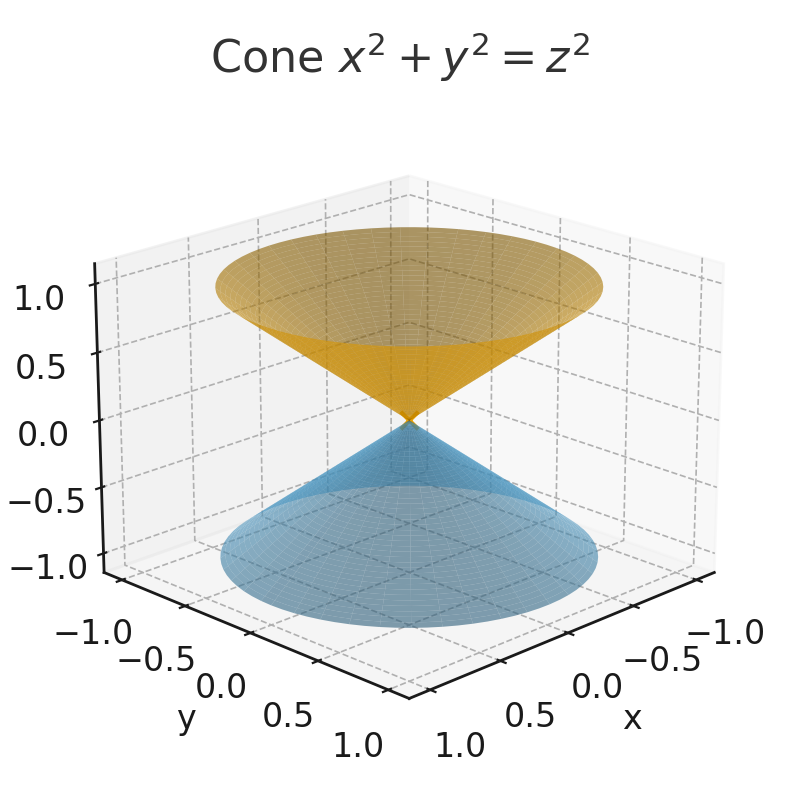
\includegraphics[width=0.55\textwidth]{chapters/part07_volume_vii/figures/cone_surface.png}
	\caption{The double cone $x^2 + y^2 = z^2$ in $\mathbb{R}^3$. 
		The apex $(0,0,0)$ is the point where the local structure 
		is not homeomorphic to an open subset of $\mathbb{R}^2$.}
	\label{fig:cone-surface}
\end{figure}

\begin{figure}[h]
	\centering
	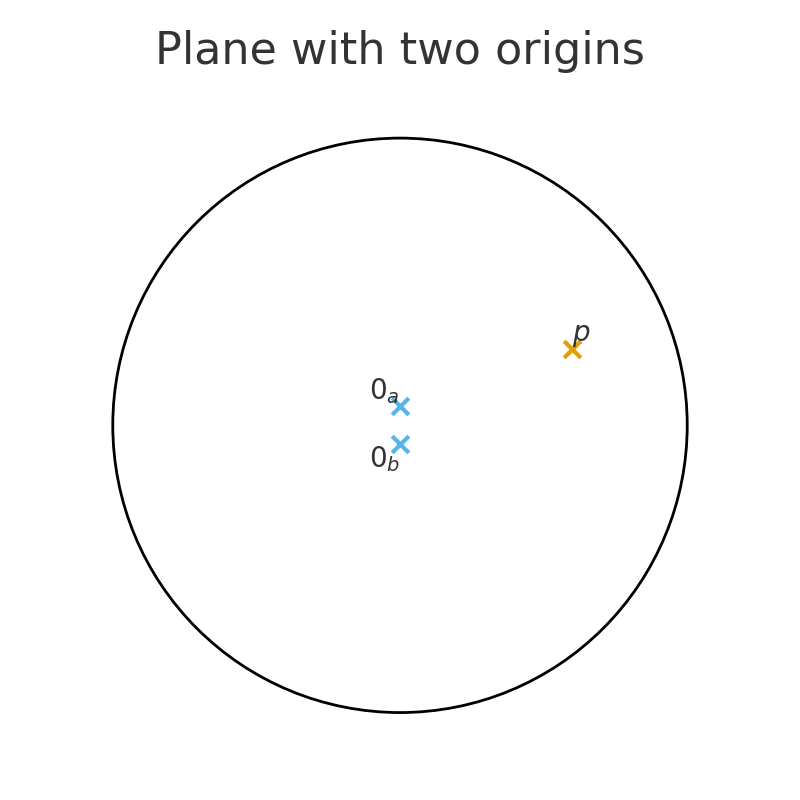
\includegraphics[width=0.4\textwidth]{chapters/part07_volume_vii/figures/plane_two_origins.png}
	\caption{Schematic picture of the ``plane with two origins'':
		all nonzero points are identified, but two distinct points 
		$0_a$ and $0_b$ remain. Any neighbourhoods of $0_a$ and $0_b$
		intersect, so the space is not Hausdorff.}
	\label{fig:plane-two-origins}
\end{figure}

\begin{figure}[h]
	\centering
	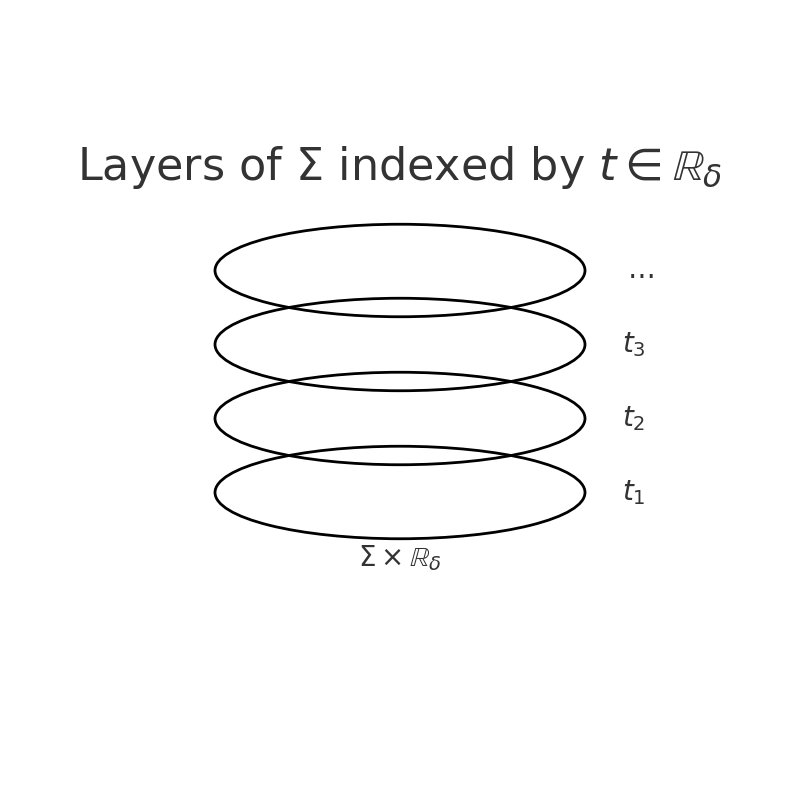
\includegraphics[width=0.45\textwidth]{chapters/part07_volume_vii/figures/sigma_times_Rdelta.png}
	\caption{Heuristic view of $\Sigma \times \mathbb{R}_\delta$ as
		an uncountable stack of copies of the surface $\Sigma$, one
		for each $t\in\mathbb{R}_\delta$. Each slice is a surface, but
		the whole space is not second countable.}
	\label{fig:sigma-times-Rdelta}
\end{figure}

\clearpage
\end{solution}

\begin{problem}[CP-VII-0003 --- Problem 3]
\label{prob:cp-vii-0003}
Draw inside the identification square for the Klein bottle $K$ the set of points
at which the `usual' map $f : K \to \mathbb{R}^{3}$
(as drawn on the right above) fails to be injective.
By considering a map
\[
h = (f,\eta) : K \longrightarrow \mathbb{R}^{3} \times \mathbb{R},
\]
where $\eta$ is a function of the width co-ordinate of the square,
explain why $K$ can be continuously embedded in $\mathbb{R}^{4}$,
i.e.\ there is a continuous map $K \to \mathbb{R}^{4}$ which is a homeomorphism
onto its image.
\emph{[You do not need an explicit formula for $f$. Many helpful pictures
	can be found at \texttt{https://en.wikipedia.org/wiki/Klein\_bottle}.]}

\par\medskip\noindent\textbf{Relevant theory: the Klein bottle}\par\smallskip


\begin{definition}[Klein bottle]
	The \emph{Klein bottle} $K$ is the quotient of the unit square
	$[0,1]\times[0,1]$ by the identifications
	\[
	(0,y) \sim (1,y) \quad \text{for all } y\in[0,1],
	\]
	and
	\[
	(x,0) \sim (1-x,1) \quad \text{for all } x\in[0,1].
	\]
	The first identification glues the left and right edges of the square with
	the same orientation, and the second glues the bottom and top edges with a
	reversal of orientation.
\end{definition}

\begin{figure}[h]
	\centering
	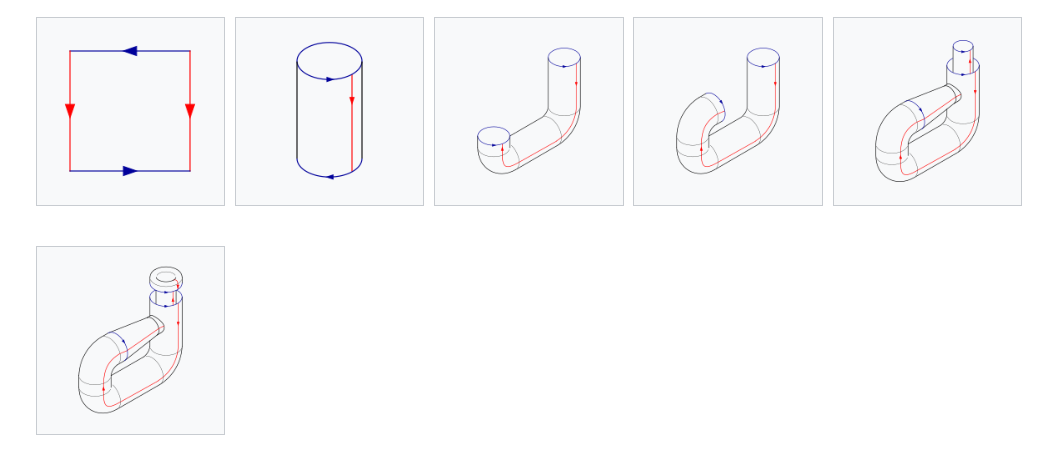
\includegraphics[width=\textwidth]{chapters/part07_volume_vii/figures/klein_construction_steps.png}
	\caption{Step--by--step construction of the usual immersed Klein bottle:
		from the identification square, through the cylinder, to the self-intersecting
		tube picture in $\mathbb{R}^3$.}
	\label{fig:klein-construction-steps}
\end{figure}


The resulting space $K$ is a closed, non-orientable surface with Euler
characteristic $\chi(K)=0$.  It is a classical fact that $K$ cannot be embedded
in $\mathbb{R}^3$ without self-intersections, but it admits an \emph{immersion}
$f : K \to \mathbb{R}^3$ whose image is the familiar ``picture'' of the Klein
bottle, where a tube passes through another part of the surface.

In this usual picture, there is a 1-dimensional subset (a closed curve) along
which the surface intersects itself.  Equivalently, there is a curve
$D \subset K$ such that $f$ is injective away from $D$, and for each
$p \in D$ the fibre $f^{-1}(f(p))$ consists of exactly two distinct points.

In terms of the square model $[0,1]\times[0,1]$, with co-ordinates $(x,y)$,
one can describe $K$ as the quotient of this square, and view the immersion
$f$ as a map which (up to the identifications) is injective except along two
distinct curves in the square that are mapped to the same curve in
$\mathbb{R}^3$.  These two curves correspond to two disjoint loops in $K$ that
meet only in their image under $f$.
\end{problem}

\begin{solution}
\par\medskip\noindent\textbf{Where $f$ fails to be injective.}\par\smallskip

By construction of the usual immersion $f : K \to \mathbb{R}^3$, there is a
closed curve in the image where the surface passes through itself.  For each
point on this self-intersection curve in $\mathbb{R}^3$, there are exactly two
distinct preimages in $K$.  Thus the set
\[
D := \{ p \in K : \# f^{-1}(f(p)) = 2 \}
\]
is a 1-dimensional subset of $K$ (topologically a circle), and $f$ is injective
on $K \setminus D$.

In the identification square $[0,1]\times[0,1]$, with co-ordinates $(x,y)$,
the set $D$ can be represented by two disjoint curves
$C_1, C_2 \subset [0,1]\times[0,1]$ which project to $D$ under the quotient
map.  Each point of $C_1$ and the corresponding point of $C_2$ (with the same
image under the quotient) is mapped by $f$ to the same point of the
self-intersection curve in $\mathbb{R}^3$.  Thus, in the quotient $K$, every
point of $D$ has exactly two preimages for $f$.

Moreover, these two preimages can be chosen to have distinct width co-ordinates:
if we write points in the square as $(x,y)$, then along the two curves
$C_1$ and $C_2$ we have
\[
(x_1(y),y) \in C_1, \qquad (x_2(y),y) \in C_2, \qquad x_1(y) \neq x_2(y),
\]
and these pairs of points project to the double points of $f$ in $K$.

\par\medskip\noindent\textbf{Construction of an embedding in $\mathbb{R}^{4}$}\par\smallskip


Let $x : K \to [0,1]/\!\sim$ denote the width co-ordinate induced from the square
model.  Choose a continuous function
\[
\eta : [0,1] \longrightarrow \mathbb{R}
\]
which is strictly monotone (for instance $\eta(t) = t$).  We can regard
$\eta$ as a continuous function on $K$ via the width co-ordinate $x$.

Define
\[
h : K \longrightarrow \mathbb{R}^3 \times \mathbb{R} \cong \mathbb{R}^4,
\qquad
h(p) := \bigl(f(p), \eta(x(p))\bigr).
\]


\begin{itemize}
	\item \emph{Continuity.}
	The map $f$ is continuous, and $\eta \circ x$ is a continuous function
	on $K$, hence $h$ is continuous.
	
	\item \emph{Injectivity.}
	Suppose $h(p_1) = h(p_2)$ for some $p_1,p_2\in K$.  Then
	\[
	f(p_1) = f(p_2)
	\quad\text{and}\quad
	\eta(x(p_1)) = \eta(x(p_2)).
	\]
	If $f(p_1) \neq f(p_2)$, we immediately have a contradiction, so assume
	$f(p_1) = f(p_2)$.  Then $p_1$ and $p_2$ must lie in the double-point set
	$D$, so they belong to the two different sheets of the self-intersection.
	In particular, they have distinct width co-ordinates:
	\[
	x(p_1) \neq x(p_2).
	\]
	Since $\eta$ is strictly monotone, it follows that
	$\eta(x(p_1)) \neq \eta(x(p_2))$, contradicting
	$\eta(x(p_1)) = \eta(x(p_2))$.  Hence such distinct $p_1,p_2$ cannot
	exist, and $h$ is injective.
	
	\item \emph{$h$ is an embedding.}
	The Klein bottle $K$ is compact, and $\mathbb{R}^4$ is Hausdorff.
	A continuous injective map from a compact space to a Hausdorff space
	is a homeomorphism onto its image.  Therefore $h$ is a topological
	embedding of $K$ into $\mathbb{R}^4$.
\end{itemize}

Thus the map $h = (f,\eta) : K \to \mathbb{R}^4$ gives a continuous embedding
of the Klein bottle into $\mathbb{R}^4$, as required.

% In the preamble:
% \usepackage{tikz}
% \usetikzlibrary{arrows.meta}

\begin{figure}[h]
	\centering
	\begin{tikzpicture}[scale=3]
		
		% The square
		\draw[thick] (0,0) rectangle (1,1);
		
		% Coordinates labels
		\node[below left] at (0,0) {$(0,0)$};
		\node[below right] at (1,0) {$(1,0)$};
		\node[above left] at (0,1) {$(0,1)$};
		\node[above right] at (1,1) {$(1,1)$};
		
		% Axes labels (width x, height y)
		\node[below] at (0.5,0) {$x$ (width)};
		\node[left] at (0,0.5) {$y$ (height)};
		
		% Horizontal edge identifications: (0,y) ~ (1,y)
		\draw[-{Latex[length=2mm]}] (0,0.2) -- (0.0,0.8);
		\draw[-{Latex[length=2mm]}] (1,0.8) -- (1.0,0.2);
		\node[left] at (0,0.5) {$\sim$};
		\node[right] at (1,0.5) {$\sim$};
		
		% Vertical edge identifications with flip: (x,0) ~ (1-x,1)
		% arrows showing opposite orientation
		\draw[-{Latex[length=2mm]}] (0.2,0) -- (0.8,0);
		\draw[-{Latex[length=2mm]}] (0.8,1.0) -- (0.2,1.0);
		\node[below] at (0.5,0) {$\sim$};
		\node[above] at (0.5,1) {$\sim$};
		
		% Two curves C1 and C2 where f is non-injective
		% (purely schematic)
		\draw[thick,blue,rounded corners=1pt]
		(0.15,0.65) .. controls (0.35,0.75) and (0.65,0.75) .. (0.85,0.65);
		
		\draw[thick,blue,rounded corners=1pt]
		(0.15,0.35) .. controls (0.35,0.25) and (0.65,0.25) .. (0.85,0.35);
		
		\node[blue] at (0.14,0.68) {$C_1$};
		\node[blue] at (0.14,0.32) {$C_2$};
		
		% Legend / explanation
		\node[align=left,anchor=west] at (1.1,0.8) {%
			\small $C_1, C_2$: two curves\\
			\small in the square that\\
			\small project to the double\\
			\small point set $D \subset K$\\
			\small where $f$ is not injective
		};
		
	\end{tikzpicture}
	\caption{Identification square for the Klein bottle and the preimage
		of the self-intersection of the usual immersion $f:K\to\mathbb{R}^3$.}
	\label{fig:klein-square-double-points}
\end{figure}

\par\medskip\noindent\textbf{1. Intuition: what you actually draw in the square}\par\smallskip


We do not need the exact formula for $f$, but conceptually:

\begin{itemize}
	\item In the usual picture in $\mathbb{R}^3$, the Klein bottle has \emph{one self-intersection circle} where a tube passes through itself.
	\item That circle comes from two \emph{distinct simple closed curves} on the surface $K$: think of them as two ``loops'' that cross in $3$--space but are disjoint on the abstract surface.
\end{itemize}

In the \emph{identification square}:

\begin{itemize}
	\item Take the square with coordinates $(x,y)\in[0,1]\times[0,1]$.
	\item Horizontal identification: $(0,y)\sim(1,y)$.
	\item Vertical identification with flip: $(x,0)\sim(1-x,1)$.
\end{itemize}

Inside this square, choose two simple curves, say

\[
C_1:\ \text{a wiggly curve roughly in the upper part}, \qquad
C_2:\ \text{a wiggly curve roughly in the lower part},
\]

such that:

\begin{itemize}
	\item They are \emph{disjoint} in the square.
	\item After applying the identifications, they become two \emph{disjoint loops in $K$}.
	\item Under the usual immersion $f$, these loops map to the \emph{same circle} in $\mathbb{R}^3$.
\end{itemize}

Therefore, the set where $f$ is not injective is:

\begin{itemize}
	\item In the \textbf{square}: the union $C_1\cup C_2$,
	\item In the \textbf{surface $K$}: the corresponding loop $D\subset K$ (a single circle, since $C_1$ and $C_2$ glue to one loop),
	\item In \textbf{$\mathbb{R}^3$}: the self-intersection circle.
\end{itemize}

Thus, when asked to ``draw inside the identification square the set of points where $f$ fails to be injective'', one literally draws the two curves $C_1$ and $C_2$ inside the square, together with the arrows showing the edge identifications.

\bigskip

\par\medskip\noindent\textbf{2. A small useful theory block: immersion vs embedding}\par\smallskip


\begin{definition}[Immersion]
	A smooth map $f : M \to \mathbb{R}^n$ from a surface $M$ is an \emph{immersion}
	if its differential has full rank at every point.  
	An immersion may have self-intersections globally.
\end{definition}

\begin{definition}[Embedding]
	A continuous map $F : M \to \mathbb{R}^n$ is a \emph{topological embedding}
	if it is continuous, injective, and a homeomorphism onto its image.
\end{definition}

For the Klein bottle:

\begin{itemize}
	\item The standard figure in $\mathbb{R}^3$ is an \emph{immersion} 
	$f : K \to \mathbb{R}^3$ with a self-intersection circle, so not an embedding.
	\item The trick with 
	\[
	h = (f,\eta) : K \to \mathbb{R}^3\times\mathbb{R}\cong\mathbb{R}^4
	\]
	is that adding the function $\eta$ (depending on the width coordinate) 
	\emph{separates the two sheets} at each double point of $f$.
\end{itemize}

Thus $h$ becomes injective, and since $K$ is compact and $\mathbb{R}^4$ is Hausdorff,
$h$ is automatically a homeomorphism onto its image---hence an \emph{embedding}.


\par\medskip\noindent\textbf{Immersions and embeddings}\par\smallskip


\begin{definition}[Immersion]
	Let $M$ be a smooth surface and $f : M \to \mathbb{R}^n$ a smooth map.
	We say that $f$ is an \emph{immersion} if its differential
	$\mathrm{d}f_p : T_pM \to T_{f(p)}\mathbb{R}^n$ has full rank
	(i.e.\ rank $2$) at every point $p\in M$.  An immersion is locally
	an embedding but it may have self-intersections globally.
\end{definition}

\begin{definition}[Embedding]
	A continuous map $F : M \to \mathbb{R}^n$ is a \emph{topological embedding}
	if it is injective and a homeomorphism onto its image $F(M)$ (with the
	subspace topology).  If $M$ is a smooth manifold and $F$ is also a smooth
	immersion, one often speaks of a \emph{smooth embedding}.
\end{definition}

For the Klein bottle $K$, the usual picture in $\mathbb{R}^3$ is given by an
immersion $f : K \to \mathbb{R}^3$ with a self-intersection curve.  The map
\[
h = (f,\eta) : K \longrightarrow \mathbb{R}^3 \times \mathbb{R}
\cong \mathbb{R}^4,
\]
with $\eta$ depending on the width co-ordinate and chosen so that distinct
points in the double point set of $f$ have distinct $\eta$-values, is a
continuous injective map.  Since $K$ is compact and $\mathbb{R}^4$ is
Hausdorff, $h$ is a homeomorphism of $K$ onto its image and thus an embedding
of $K$ into $\mathbb{R}^4$.

\begin{definition}[Topological embedding]
	A continuous map $F : M \to \mathbb{R}^n$ is a \emph{topological embedding}
	if it is injective and a homeomorphism onto its image $F(M)$
	(with the subspace topology).
	If $F$ is also a smooth immersion, one often calls it a \emph{smooth embedding}.
\end{definition}

\par\medskip\noindent\textbf{Immersion of the Klein bottle in $\mathbb{R}^3$.}\par\smallskip

The familiar picture of the Klein bottle in $\mathbb{R}^3$ is obtained from a
smooth map
\[
f : K \longrightarrow \mathbb{R}^3,
\]
constructed by gluing a cylinder with a twist. 
This map is a smooth immersion: near every point of $K$, the surface looks
locally like an embedded surface in $\mathbb{R}^3$.  
However, globally $f(K)$ contains a self-intersection curve where one tube
passes through another.  
Hence $f$ is \emph{not} an embedding, because
\[
\# f^{-1}(q) = 2 \quad \text{for all } q \text{ on the self-intersection circle}.
\]

\par\medskip\noindent\textbf{Separating the double points in higher dimension.}\par\smallskip

The obstruction to embedding $K$ into $\mathbb{R}^3$ lies entirely in these
double points.  
If we could assign an additional coordinate that takes \emph{different values}
on the two preimages of every self-intersection point, then the map would
become injective.

This is accomplished by introducing a fourth coordinate that depends only on
the width co-ordinate of the square model of $K$.  
This leads to a map
\[
h = (f,\eta) : K \longrightarrow \mathbb{R}^3 \times \mathbb{R}
\cong \mathbb{R}^4,
\]
which is injective and hence (by compactness of $K$ and Hausdorffness of
$\mathbb{R}^4$) a topological embedding.

Thus the Klein bottle, although not embeddable in $\mathbb{R}^3$, embeds
smoothly and naturally in $\mathbb{R}^4$.
\end{solution}

\begin{problem}[CP-VII-0004 --- Problem E1 --- Map Colouring on Surfaces]
\label{prob:cp-vii-0004}
\begin{enumerate}[label=\textnormal{(\alph*)}]
	
	\item
	View a polygonal decomposition of a topological surface $S$ with all
	vertices of valence $\ge 3$ as a map drawn on $S$.
	The map can be coloured with $N$ colours if we can colour faces so that
	faces which share an edge have different colours (but faces which meet
	only at a vertex may have the same colour).
	
	Suppose that $N \in \mathbb{N}$ is a positive integer such that
	\[
	\frac{2E}{F} < N
	\]
	for every possible decomposition of $S$ (here $E$ is the number of edges
	and $F$ the number of faces).
	Show that every map on $S$ can be coloured with at most $N$ colours.
	\emph{[Hint: Induct on $F$, noting that the result is straightforward if
		$F < N$.]}
	
	\item
	Prove that for any decomposition of $S$ (where all vertices have valence
	at least $3$), we have
	\[
	\frac{2E}{F} \le 6\Bigl(1 - \frac{\chi(S)}{F}\Bigr),
	\]
	where $\chi(S)$ is the Euler characteristic of $S$.
	Deduce that any map on a torus can be coloured with $7$ colours.
	
	The map on the torus depicted below can be coloured with $7$ colours but
	not fewer -- why?
	\emph{[The black dots represent the vertices; note the `corner' of the
		rectangle is not one.]}
	
\end{enumerate}

\begin{figure}[h]
	\centering
	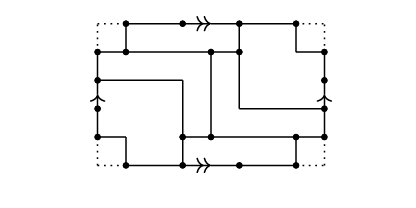
\includegraphics[width=0.7\textwidth]{chapters/part07_volume_vii/figures/e1.png}%
	\caption{A map on the torus used in part (b) of Problem E1.
		The black dots represent the vertices; the corner of the rectangle is
		not a vertex.}
	\label{fig:E1-torus-map}
\end{figure}

\par\medskip\noindent\textbf{Valence (Degree) of a Vertex}\par\smallskip


Let $G$ be the graph coming from a polygonal decomposition of a surface $S$,
with vertex set $V$ and edge set $E$.

\begin{definition}
	For a vertex $v \in V$, the \emph{valence} (or \emph{degree}) of $v$,
	denoted $\operatorname{val}(v)$, is the number of edges of $G$ which are
	incident with $v$.
	Equivalently, $\operatorname{val}(v)$ is the number of polygon edges that
	meet at $v$ in the decomposition.
\end{definition}

Thus, if three polygon edges meet at a point $v$, then $\operatorname{val}(v)=3$;
if four edges meet at $v$, then $\operatorname{val}(v)=4$, and so on.
(Loops, i.e.\ edges that begin and end at the same vertex, are counted
twice, but such edges usually do not appear in polygonal decompositions.)

In the context of map colouring problems, one usually assumes that all
vertices have valence at least $3$.  This excludes degenerate configurations
and ensures that each vertex is surrounded by at least three faces, so that
Euler characteristic and counting arguments behave nicely.
	
	
	\begin{figure}[h]
		\centering
		
		%%%%% Vertex of valence 3 %%%%%
		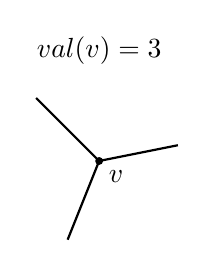
\begin{tikzpicture}[scale=1]
			\node at (0,1.4) {$\operatorname{val}(v)=3$};
			\fill (0,0) circle (0.05) node[below right] {$v$};
			\draw[thick] (0,0) -- (1,0.2);
			\draw[thick] (0,0) -- (-0.8,0.8);
			\draw[thick] (0,0) -- (-0.4,-1.0);
		\end{tikzpicture}
		\hspace{1.5cm}
		%%%%% Vertex of valence 4 %%%%%
		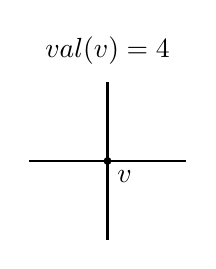
\begin{tikzpicture}[scale=1]
			\node at (0,1.4) {$\operatorname{val}(v)=4$};
			\fill (0,0) circle (0.05) node[below right] {$v$};
			\draw[thick] (0,0) -- (1,0);
			\draw[thick] (0,0) -- (-1,0);
			\draw[thick] (0,0) -- (0,1);
			\draw[thick] (0,0) -- (0,-1);
		\end{tikzpicture}
		\hspace{1.5cm}
		%%%%% Vertex of valence 5 %%%%%
		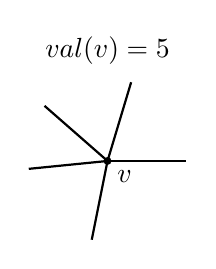
\begin{tikzpicture}[scale=1]
			\node at (0,1.4) {$\operatorname{val}(v)=5$};
			\fill (0,0) circle (0.05) node[below right] {$v$};
			\draw[thick] (0,0) -- (1,0);
			\draw[thick] (0,0) -- (0.3,1.0);
			\draw[thick] (0,0) -- (-0.8,0.7);
			\draw[thick] (0,0) -- (-1.0,-0.1);
			\draw[thick] (0,0) -- (-0.2,-1.0);
		\end{tikzpicture}
		
		\caption{Examples of vertices of valence $3$, $4$, and $5$.
			The valence of a vertex is the number of incident edges.}
		\label{fig:vertex-valences}
	\end{figure}
	
	
\par\medskip\noindent\textbf{Euler Characteristic}\par\smallskip


Let $S$ be a surface equipped with a polygonal (or triangulated)
decomposition.
Denote by $V$ the number of vertices, by $E$ the number of edges, and by
$F$ the number of faces (2--cells).

\begin{definition}
	The \emph{Euler characteristic} of $S$ is
	\[
	\chi(S) := V - E + F.
	\]
	A fundamental theorem of topology says that $\chi(S)$ is independent of the
	chosen polygonal decomposition: it is a topological invariant of the
	surface $S$.
\end{definition}

\par\medskip\noindent\textbf{Examples}\par\smallskip


\par\medskip\noindent\textbf{Sphere $S^2$.}\par\smallskip

Consider a tetrahedron drawn on the sphere.  It has
$V=4$ vertices, $E=6$ edges and $F=4$ triangular faces, so
\[
\chi(S^2) = V - E + F = 4 - 6 + 4 = 2.
\]

\par\medskip\noindent\textbf{Torus $T^2$.}\par\smallskip

Represent the torus as a square with opposite sides identified.
Using the standard cell structure, there is
one vertex (all four corners are identified), two edges (one horizontal and
one vertical loop), and one face (the interior of the square).  Hence
\[
\chi(T^2) = 1 - 2 + 1 = 0.
\]

More generally, a closed orientable surface of genus $g$ satisfies
\[
\chi(\Sigma_g) = 2 - 2g.
\]
In particular $S^2$ (genus $0$) has Euler characteristic $2$, the torus
(genus $1$) has Euler characteristic $0$, a double torus (genus $2$) has
Euler characteristic $-2$, and so on.
	
	\begin{figure}[h]
		\centering
		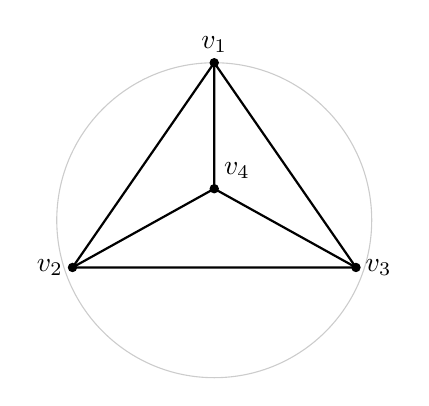
\begin{tikzpicture}[scale=2]
			
			% sphere outline (just for intuition)
			\draw[gray!40] (0,0) circle (1);
			
			% tetrahedron vertices
			\coordinate (A) at (0,1);
			\coordinate (B) at (-0.9,-0.3);
			\coordinate (C) at (0.9,-0.3);
			\coordinate (D) at (0,0.2);
			
			% edges
			\draw[thick] (A)--(B)--(C)--(A);   % outer triangle
			\draw[thick] (A)--(D)--(B);
			\draw[thick] (C)--(D);
			
			% vertices
			\fill (A) circle (0.03) node[above] {$v_1$};
			\fill (B) circle (0.03) node[left] {$v_2$};
			\fill (C) circle (0.03) node[right] {$v_3$};
			\fill (D) circle (0.03) node[above right] {$v_4$};
			
		\end{tikzpicture}
		\caption{A tetrahedron drawn on $S^2$.  Here $V=4$, $E=6$, $F=4$ and
			$\chi(S^2)=4-6+4=2$.}
		\label{fig:euler-sphere}
	\end{figure}
	
	\begin{figure}[h]
		\centering
		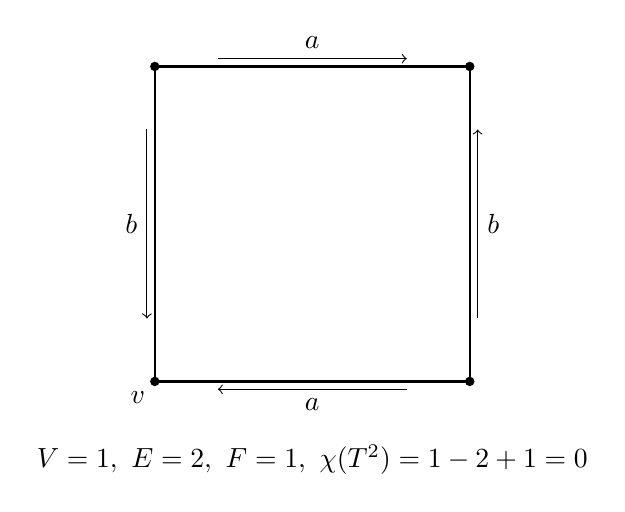
\begin{tikzpicture}[scale=2]
			
			% square
			\draw[thick] (-1,-1) rectangle (1,1);
			
			% arrows indicating identifications
			\draw[->] (-0.6,1.05) -- (0.6,1.05);
			\draw[->] (0.6,-1.05) -- (-0.6,-1.05);
			\node[above] at (0,1.05) {$a$};
			\node[below] at (0,-1.05) {$a$};
			
			\draw[->] (1.05,-0.6) -- (1.05,0.6);
			\draw[->] (-1.05,0.6) -- (-1.05,-0.6);
			\node[right] at (1.05,0) {$b$};
			\node[left]  at (-1.05,0) {$b$};
			
			% single vertex (all corners identified)
			\fill (-1,-1) circle (0.03);
			\fill (1,-1) circle (0.03);
			\fill (1,1) circle (0.03);
			\fill (-1,1) circle (0.03);
			\node[below left] at (-1,-1) {$v$};
			
			% label
			\node at (0,-1.5) {$V=1,\ E=2,\ F=1,\ \chi(T^2)=1-2+1=0$};
			
		\end{tikzpicture}
		\caption{Square with opposite edges identified, giving the torus $T^2$.
			All four corners represent the same vertex $v$, the two independent edge
			loops are labelled $a$ and $b$, and the whole interior is a single face.}
		\label{fig:euler-torus}
	\end{figure}
	
	\begin{figure}[h]
		\centering
		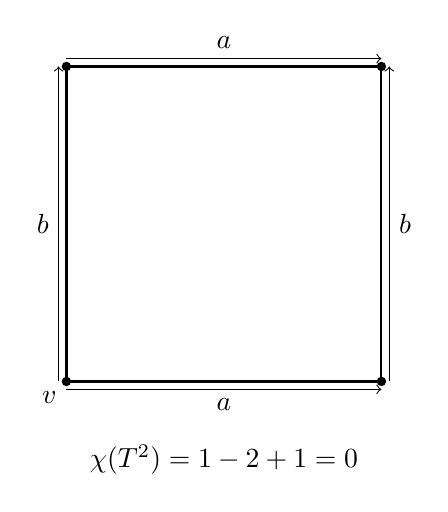
\begin{tikzpicture}[scale=2]
			
			% square
			\draw[thick] (-1,-1) rectangle (1,1);
			
			% horizontal edges (a)
			\draw[->] (-1,1.05) -- (1,1.05);
			\draw[->] (-1,-1.05) -- (1,-1.05);
			\node[above] at (0,1.05) {$a$};
			\node[below] at (0,-1.05) {$a$};
			
			% vertical edges (b)
			\draw[->] (1.05,-1) -- (1.05,1);
			\draw[->] (-1.05,-1) -- (-1.05,1);
			\node[right] at (1.05,0) {$b$};
			\node[left]  at (-1.05,0) {$b$};
			
			% all four corners identified as one vertex
			\fill (-1,-1) circle (0.03);
			\fill (1,-1) circle (0.03);
			\fill (1,1) circle (0.03);
			\fill (-1,1) circle (0.03);
			\node[below left] at (-1,-1) {$v$};
			
			\node at (0,-1.5) {$\chi(T^2) = 1 - 2 + 1 = 0$};
			
		\end{tikzpicture}
		\caption{Square with opposite sides identified to form the torus $T^2$.
			Although opposite edges are drawn with arrows in the same direction, the
			boundary word is $aba^{-1}b^{-1}$ when read anticlockwise.}
		\label{fig:torus-fundamental-square}
	\end{figure}
	
	\begin{figure}[h]
		\centering
		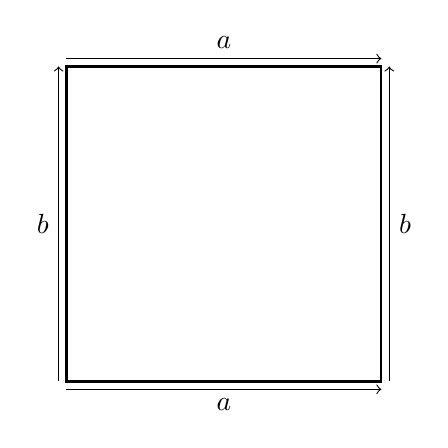
\begin{tikzpicture}[scale=2]
			
			% square
			\draw[thick] (-1,-1) rectangle (1,1);
			
			% horizontal edges labelled a
			\draw[->] (-1,1.05) -- (1,1.05);
			\draw[->] (-1,-1.05) -- (1,-1.05);
			\node[above] at (0,1.05) {$a$};
			\node[below] at (0,-1.05) {$a$};
			
			% vertical edges labelled b
			\draw[->] (1.05,-1) -- (1.05,1);
			\draw[->] (-1.05,-1) -- (-1.05,1);
			\node[right] at (1.05,0) {$b$};
			\node[left]  at (-1.05,0) {$b$};
			
		\end{tikzpicture}
		\caption{Fundamental polygon for the torus. Traversing anticlockwise produces the word $a\,b\,a^{-1}\,b^{-1}$.}
	\end{figure}
	
	
	\begin{figure}[h]
		\centering
		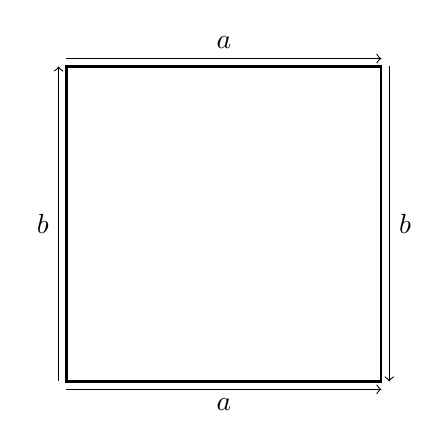
\begin{tikzpicture}[scale=2]
			
			% square
			\draw[thick] (-1,-1) rectangle (1,1);
			
			% horizontal edges labelled a (same orientation)
			\draw[->] (-1,1.05) -- (1,1.05);
			\draw[->] (-1,-1.05) -- (1,-1.05);
			\node[above] at (0,1.05) {$a$};
			\node[below] at (0,-1.05) {$a$};
			
			% vertical edges labelled b, one arrow reversed
			\draw[->] (1.05,1) -- (1.05,-1);      % downward arrow
			\draw[->] (-1.05,-1) -- (-1.05,1);    % upward arrow
			\node[right] at (1.05,0) {$b$};
			\node[left]  at (-1.05,0) {$b$};
			
		\end{tikzpicture}
		\caption{Fundamental polygon for the Klein bottle. Traversal yields $a\,b\,a\,b^{-1}$.}
	\end{figure}
	
	\clearpage
	
	\par\medskip\noindent\textbf{Real projective plane $\mathbb{RP}^2$}\par\smallskip

	
	The real projective plane $\mathbb{RP}^2$ can be obtained from a square by
	identifying each pair of opposite edges with reversed orientation.
	A standard cell decomposition has
	\[
	V = 1,\quad E = 1,\quad F = 1,
	\]
	so
	\[
	\chi(\mathbb{RP}^2) = V - E + F = 1 - 1 + 1 = 1.
	\]
	
	\begin{figure}[h]
		\centering
		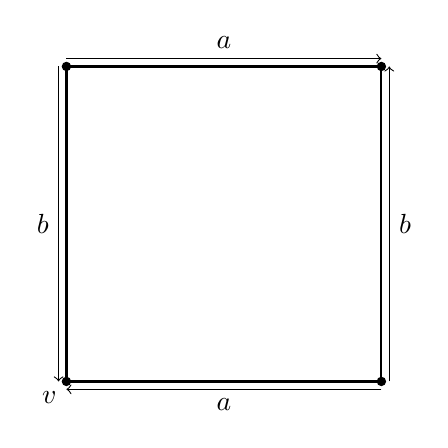
\begin{tikzpicture}[scale=2]
			
			% square
			\draw[thick] (-1,-1) rectangle (1,1);
			
			% horizontal edges (label a, opposite directions)
			\draw[->] (-1,1.05) -- (1,1.05);
			\draw[->] (1,-1.05) -- (-1,-1.05);
			\node[above] at (0,1.05) {$a$};
			\node[below] at (0,-1.05) {$a$};
			
			% vertical edges (label b, opposite directions)
			\draw[->] (1.05,-1) -- (1.05,1);
			\draw[->] (-1.05,1) -- (-1.05,-1);
			\node[right] at (1.05,0) {$b$};
			\node[left]  at (-1.05,0) {$b$};
			
			% corners all identified as one vertex
			\fill (-1,-1) circle (0.03);
			\fill (1,-1) circle (0.03);
			\fill (1,1) circle (0.03);
			\fill (-1,1) circle (0.03);
			\node[below left] at (-1,-1) {$v$};
			
		\end{tikzpicture}
		\caption{Fundamental polygon for $\mathbb{RP}^2$: opposite edges are identified
			with reversed orientation. In a suitable cell decomposition one obtains
			$V=1$, $E=1$, $F=1$ and hence $\chi(\mathbb{RP}^2)=1$.}
		\label{fig:rp2-fundamental}
	\end{figure}
	
	\par\medskip\noindent\textbf{Klein bottle $K$}\par\smallskip

	
	The Klein bottle can be represented by a square whose horizontal edges are
	identified with the same orientation and whose vertical edges are
	identified with opposite orientation.  A convenient cell decomposition has
	\[
	V = 1,\quad E = 2,\quad F = 1,
	\]
	so
	\[
	\chi(K) = 1 - 2 + 1 = 0.
	\]
	Although the Euler characteristic agrees with that of the torus, the Klein
	bottle is non-orientable and thus not homeomorphic to $T^2$.
	
	\begin{figure}[h]
		\centering
		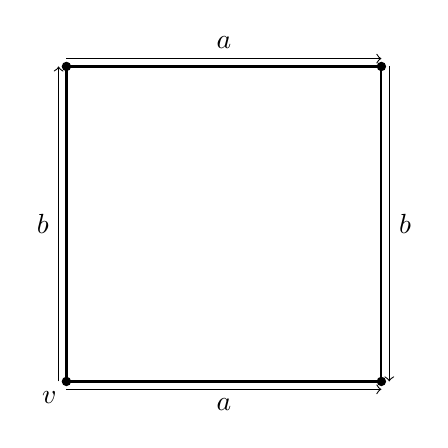
\begin{tikzpicture}[scale=2]
			
			% square
			\draw[thick] (-1,-1) rectangle (1,1);
			
			% horizontal edges (a, same direction)
			\draw[->] (-1,1.05) -- (1,1.05);
			\draw[->] (-1,-1.05) -- (1,-1.05);
			\node[above] at (0,1.05) {$a$};
			\node[below] at (0,-1.05) {$a$};
			
			% vertical edges (b, opposite directions)
			\draw[->] (1.05,1) -- (1.05,-1);
			\draw[->] (-1.05,-1) -- (-1.05,1);
			\node[right] at (1.05,0) {$b$};
			\node[left]  at (-1.05,0) {$b$};
			
			% corners identified
			\fill (-1,-1) circle (0.03);
			\fill (1,-1) circle (0.03);
			\fill (1,1) circle (0.03);
			\fill (-1,1) circle (0.03);
			\node[below left] at (-1,-1) {$v$};
			
		\end{tikzpicture}
		\caption{Fundamental polygon for the Klein bottle $K$: one pair of edges
			is identified with the same orientation, the other pair with reversed
			orientation. A suitable cell structure yields $V=1$, $E=2$, $F=1$ and
			$\chi(K)=0$.}
		\label{fig:klein-fundamental}
	\end{figure}
	
	\par\medskip\noindent\textbf{Double torus $\Sigma_2$}\par\smallskip

	
	A closed orientable surface of genus $2$ (a ``double torus'') can be
	represented by an octagon whose edges are labelled
	\[
	a, b, a^{-1}, b^{-1}, c, d, c^{-1}, d^{-1}
	\]
	in order around the boundary.
	All $8$ vertices are identified to a single vertex, and the $8$ edges form
	$4$ pairs corresponding to the loops $a,b,c,d$.  There is a single face
	(the interior of the octagon).  Thus
	\[
	V = 1,\quad E = 4,\quad F = 1,
	\]
	and
	\[
	\chi(\Sigma_2) = 1 - 4 + 1 = -2.
	\]
	This agrees with the general formula for closed orientable surfaces of
	genus $g$:
	\[
	\chi(\Sigma_g) = 2 - 2g.
	\]
	
	\begin{figure}[h]
		\centering
		\begin{tikzpicture}[scale=1.4]
			
			% vertices of an octagon
			\coordinate (P1) at (1,0);
			\coordinate (P2) at (0.3,0.8);
			\coordinate (P3) at (-0.3,0.8);
			\coordinate (P4) at (-1,0);
			\coordinate (P5) at (-0.8,-0.6);
			\coordinate (P6) at (-0.2,-1);
			\coordinate (P7) at (0.2,-1);
			\coordinate (P8) at (0.8,-0.6);
			
			% draw octagon
			\draw[thick] (P1)--(P2)--(P3)--(P4)--(P5)--(P6)--(P7)--(P8)--cycle;
			
			% edge labels (schematic)
			\node[above right] at ($(P1)!0.5!(P2)$) {$a$};
			\node[above]       at ($(P2)!0.5!(P3)$) {$b$};
			\node[above left]  at ($(P3)!0.5!(P4)$) {$a^{-1}$};
			\node[left]        at ($(P4)!0.5!(P5)$) {$b^{-1}$};
			\node[below left]  at ($(P5)!0.5!(P6)$) {$c$};
			\node[below]       at ($(P6)!0.5!(P7)$) {$d$};
			\node[below right] at ($(P7)!0.5!(P8)$) {$c^{-1}$};
			\node[right]       at ($(P8)!0.5!(P1)$) {$d^{-1}$};
			
			% all vertices identified: indicate single vertex
			\fill (P1) circle (0.03);
			\fill (P2) circle (0.03);
			\fill (P3) circle (0.03);
			\fill (P4) circle (0.03);
			\fill (P5) circle (0.03);
			\fill (P6) circle (0.03);
			\fill (P7) circle (0.03);
			\fill (P8) circle (0.03);
			\node[right] at (P1) {$v$};
			
		\end{tikzpicture}
		\caption{Fundamental polygon for the genus $2$ surface $\Sigma_2$.
			All $8$ vertices are identified to a single vertex $v$, the $8$ edges form
			$4$ pairs, and the interior is one face, giving $V=1$, $E=4$, $F=1$ and
			$\chi(\Sigma_2) = -2$.}
		\label{fig:double-torus-fundamental}
	\end{figure}
	
	\par\medskip\noindent\textbf{Euler characteristic and the inequality in E1(b)}\par\smallskip

	
	Let $S$ be a surface with a polygonal decomposition in which every vertex
	has valence at least $3$.  Denote by $V,E,F$ the numbers of vertices,
	edges and faces respectively, and let $\chi(S) = V - E + F$ be the Euler
	characteristic of $S$.
	
	Write $V_m$ for the number of vertices of valence $m$.  Then
	\[
	\sum_m V_m = V,
	\qquad
	\sum_m mV_m = 2E,
	\]
	and the assumption on valences implies $V_m=0$ for $m<3$.  Hence
	\[
	2E = \sum_m mV_m \;\ge\; \sum_m 3V_m = 3V,
	\]
	so that
	\[
	V \le \frac{2E}{3}.
	\]
	
	On the other hand, the Euler characteristic may be written as
	\[
	\chi(S) = V - E + F
	\quad\Longrightarrow\quad
	F - \chi(S) = E - V.
	\]
	Multiplying by $2$ gives
	\[
	2(F - \chi(S)) = 2E - 2V.
	\]
	Using the bound $V \le 2E/3$ we obtain
	\[
	2E - 2V \;\ge\; 2E - 2\cdot\frac{2E}{3}
	= \frac{2E}{3},
	\]
	and hence
	\[
	2(F - \chi(S)) \;\ge\; \frac{2E}{3}
	\quad\Longrightarrow\quad
	F - \chi(S) \;\ge\; \frac{E}{3}.
	\]
	Equivalently,
	\[
	E \le 3\bigl(F - \chi(S)\bigr).
	\]
	Multiplying both sides by $2/F$ yields
	\[
	\frac{2E}{F} \;\le\;
	\frac{6(F - \chi(S))}{F}
	= 6\Bigl(1 - \frac{\chi(S)}{F}\Bigr),
	\]
	which is precisely the inequality stated in part~(b) of Problem~E1.
	
	\par\medskip\noindent\textbf{Colouring bounds for the sphere and the torus}\par\smallskip

	
	Part~(a) of Problem~E1 shows that if there exists an integer $N$ such that
	\[
	\frac{2E}{F} < N
	\]
	for every polygonal decomposition of $S$ (with all vertices of valence
	$\ge 3$), then every map on $S$ can be coloured with at most $N$ colours.
	
	For the sphere $S^2$ we have $\chi(S^2)=2$, and the inequality above
	gives
	\[
	\frac{2E}{F} \le 6\Bigl(1 - \frac{2}{F}\Bigr) < 6
	\]
	for every decomposition.  Thus we may take $N=6$, and every map on $S^2$
	is $6$--colourable (this is the classical six-colour theorem).
	
	For the torus $T^2$ we have $\chi(T^2)=0$, so the inequality reduces to
	\[
	\frac{2E}{F} \le 6.
	\]
	Hence any $N>6$ satisfies $\frac{2E}{F} < N$ for all decompositions; in
	particular we may choose $N=7$ and conclude that every map on the torus is
	$7$--colourable.  The specific example drawn in Problem~E1 shows a map on
	the torus which cannot be coloured with fewer than $7$ colours, so this
	bound is sharp.
	
	\clearpage
	
	\par\medskip\noindent\textbf{Examples of Euler characteristics}\par\smallskip

	
	For reference, the Euler characteristics of some standard closed surfaces
	are collected in Table~\ref{tab:euler-surfaces}.
	
	\begin{table}[h]
		\centering
		\begin{tabular}{lcc}
			\hline
			Surface $S$ & Description & $\chi(S)$ \\
			\hline
			$S^2$ & sphere (genus $0$)          & $2$ \\
			$T^2$ & torus (genus $1$)           & $0$ \\
			$\Sigma_2$ & double torus (genus $2$) & $-2$ \\
			$\mathbb{RP}^2$ & real projective plane & $1$ \\
			$K$ & Klein bottle                  & $0$ \\
			\hline
		\end{tabular}
		\caption{Euler characteristics of some standard closed surfaces.}
		\label{tab:euler-surfaces}
	\end{table}
\end{problem}

\begin{solution}
We prove the statement by induction on the number of faces $F$ in the map.
	
	Recall that a map on $S$ is given by a polygonal decomposition with $V$
	vertices, $E$ edges and $F$ faces, and that by assumption there exists a
	fixed integer $N \in \mathbb{N}$ such that
	\[
	\frac{2E}{F} < N
	\]
	for every such decomposition of $S$.
	
	\par\medskip\noindent\textbf{Base case: $F < N$.}\par\smallskip

	Suppose first that $F < N$.
	The adjacency graph of faces has at most $F$ vertices, and each face has
	at most $F-1$ neighbours (it cannot share an edge with itself).
	We can therefore colour the faces greedily with $N$ colours as follows:
	list the faces as $F_1,\dots,F_F$, and colour them one by one.
	When we come to colour $F_k$, at most $k-1 \le F-1 < N$ neighbours have
	already been assigned colours, so at most $N-1$ colours are forbidden.
	Since there are $N$ colours available, at least one colour remains,
	and we may assign it to $F_k$.
	Thus any map with $F < N$ is $N$--colourable.
	
	\par\medskip\noindent\textbf{Inductive step.}\par\smallskip

	Assume now that every map on $S$ with fewer than $F$ faces is
	$N$--colourable, and let $M$ be a map on $S$ with $F$ faces, $E$ edges,
	and satisfying
	\[
	\frac{2E}{F} < N.
	\]
	We must show that $M$ is $N$--colourable.
	
	Let $F_n$ denote the number of faces of $M$ which are bounded by exactly
	$n$ edges.  Then
	\[
	F = \sum_n F_n,
	\qquad
	\sum_n nF_n = 2E,
	\]
	since each edge is incident with exactly two faces.
	Hence the average number of edges per face is
	\[
	\frac{1}{F}\sum_n nF_n
	= \frac{2E}{F}
	< N.
	\]
	If every face had at least $N$ edges, then the average would be at least
	$N$, which contradicts the inequality above.
	Therefore there exists at least one face $f$ which has at most $N-1$
	edges.
	
	Remove this face $f$ from the map, leaving a new map $M'$ on $S$ with
	\[
	F' = F-1
	\]
	faces.  (Some edges may now bound only one face, but this does not affect
	the argument.)
	By the hypothesis on $N$, the inequality
	\[
	\frac{2E'}{F'} < N
	\]
	holds for \emph{every} decomposition of $S$, and in particular for $M'$.
	Thus, by the inductive hypothesis, $M'$ is $N$--colourable.
	
	Consider the face $f$ which we removed.  It is incident with at most
	$N-1$ distinct neighbouring faces (since it has at most $N-1$ edges), and
	these neighbours are already coloured in $M'$.
	Among the $N$ available colours, at most $N-1$ are used on these
	neighbours, so there is at least one colour which does not appear among
	them.
	Assign such a colour to $f$.
	Then adjacent faces always have distinct colours, and we have obtained an
	$N$--colouring of the original map $M$.
	
	By induction on $F$, every map on $S$ can be coloured with at most $N$
	colours.

	
	\begin{figure}[h]
		\centering
		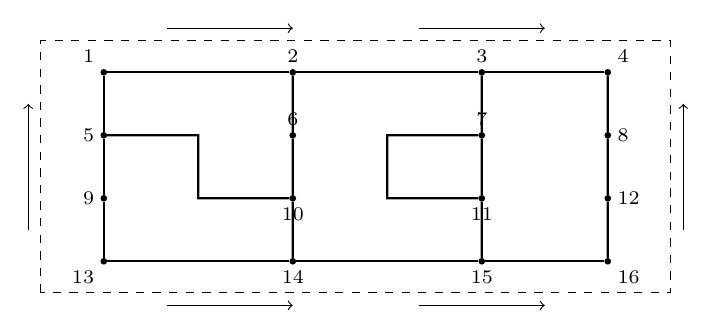
\begin{tikzpicture}[scale=0.8, every node/.style={font=\scriptsize}]
			
			% Fundamental rectangle (torus)
			\draw[dashed] (0,0) rectangle (10,4);
			
			% Identification arrows (left-right)
			\draw[->] (2,4.2) -- (4,4.2);
			\draw[->] (6,4.2) -- (8,4.2);
			\draw[->] (2,-0.2) -- (4,-0.2);
			\draw[->] (6,-0.2) -- (8,-0.2);
			
			% Identification arrows (bottom-top)
			\draw[->] (-0.2,1) -- (-0.2,3);
			\draw[->] (10.2,1) -- (10.2,3);
			
			% --- vertices (roughly matching a 7-hexagon tiling) ---
			
			% top row
			\node[inner sep=1pt] (v1)  at (1,3.5)  {};
			\node[inner sep=1pt] (v2)  at (4,3.5)  {};
			\node[inner sep=1pt] (v3)  at (7,3.5)  {};
			\node[inner sep=1pt] (v4)  at (9,3.5)  {};
			
			% upper middle row
			\node[inner sep=1pt] (v5)  at (1,2.5)  {};
			\node[inner sep=1pt] (v6)  at (4,2.5)  {};
			\node[inner sep=1pt] (v7)  at (7,2.5)  {};
			\node[inner sep=1pt] (v8)  at (9,2.5)  {};
			
			% lower middle row
			\node[inner sep=1pt] (v9)  at (1,1.5)  {};
			\node[inner sep=1pt] (v10) at (4,1.5)  {};
			\node[inner sep=1pt] (v11) at (7,1.5)  {};
			\node[inner sep=1pt] (v12) at (9,1.5)  {};
			
			% bottom row
			\node[inner sep=1pt] (v13) at (1,0.5)  {};
			\node[inner sep=1pt] (v14) at (4,0.5)  {};
			\node[inner sep=1pt] (v15) at (7,0.5)  {};
			\node[inner sep=1pt] (v16) at (9,0.5)  {};
			
			% draw the dots
			\foreach \v in {1,...,16}{
				\fill (v\v) circle (1.5pt);
			}
			
			% labels (you can shift them slightly if needed)
			\node[above left]  at (v1)  {$1$};
			\node[above]       at (v2)  {$2$};
			\node[above]       at (v3)  {$3$};
			\node[above right] at (v4)  {$4$};
			
			\node[left]        at (v5)  {$5$};
			\node[above]       at (v6)  {$6$};
			\node[above]       at (v7)  {$7$};
			\node[right]       at (v8)  {$8$};
			
			\node[left]        at (v9)  {$9$};
			\node[below]       at (v10) {$10$};
			\node[below]       at (v11) {$11$};
			\node[right]       at (v12) {$12$};
			
			\node[below left]  at (v13) {$13$};
			\node[below]       at (v14) {$14$};
			\node[below]       at (v15) {$15$};
			\node[below right] at (v16) {$16$};
			
			% --- edges (just a schematic network) ---
			
			% top zig-zag
			\draw[thick] (v1) -- (v2) -- (v3) -- (v4);
			% left verticals
			\draw[thick] (v1) -- (v5) -- (v9) -- (v13);
			% middle verticals
			\draw[thick] (v2) -- (v6) -- (v10) -- (v14);
			\draw[thick] (v3) -- (v7) -- (v11) -- (v15);
			% right verticals
			\draw[thick] (v4) -- (v8) -- (v12) -- (v16);
			% bottom zig-zag
			\draw[thick] (v13) -- (v14) -- (v15) -- (v16);
			
			% two interior ``bends'' to suggest the hexagonal regions
			\draw[thick] (v5) -- (2.5,2.5) -- (2.5,1.5) -- (v10);
			\draw[thick] (v7) -- (5.5,2.5) -- (5.5,1.5) -- (v11);
			
		\end{tikzpicture}
		\caption{A schematic torus map with vertices labelled.
			The left/right and top/bottom edges of the rectangle are identified.}
		\label{fig:torus-map-labelled}
	\end{figure}
	
	\clearpage
	
\par\medskip\noindent\textbf{The Real Projective Plane \texorpdfstring{$\mathbb{RP}^2$}{RP2}}\par\smallskip


\par\medskip\noindent\textbf{Definitions of $\mathbb{RP}^2$}\par\smallskip


There are several equivalent ways to define the real projective plane.  
Each illuminates a different geometric property of $\mathbb{RP}^2$.

\begin{definition}[As Lines Through the Origin in $\mathbb{R}^3$]
	The real projective plane is the space of 1-dimensional linear subspaces of
	$\mathbb{R}^3$.  Two nonzero vectors $v,w \in \mathbb{R}^3$ represent the same
	point of $\mathbb{RP}^2$ if $w = \lambda v$ for some nonzero real number
	$\lambda$.  
	
	Every point of $\mathbb{RP}^2$ may be written using homogeneous coordinates:
	\[
	[x:y:z] = [\lambda x : \lambda y : \lambda z], \qquad \lambda \neq 0.
	\]
	
	Thus
	\[
	\mathbb{RP}^2 = (\mathbb{R}^3 \setminus \{0\}) / \!\sim ,
	\qquad v \sim w \Longleftrightarrow w = \lambda v \text{ for some } \lambda \ne 0.
	\]
\end{definition}

\begin{definition}[Affine Plane with Line at Infinity]
	Embed the affine plane $\mathbb{R}^2$ into projective space by
	\[
	(x,y) \longmapsto [x : y : 1].
	\]
	The points with $z=0$ are the \emph{points at infinity}:
	\[
	[x : y : 0] \in \mathbb{RP}^2 \setminus \mathbb{R}^2.
	\]
	They represent directions of parallel lines in the affine plane.
	
	Therefore,
	\[
	\mathbb{RP}^2 = \mathbb{R}^2 \ \cup\  \mathbb{RP}^1,
	\]
	where $\mathbb{RP}^1$ is the \emph{projective line at infinity}.
\end{definition}

\begin{definition}[Sphere Modulo Antipodal Identification]
	Let
	\[
	S^2 = \{ (x,y,z)\in\mathbb{R}^3 : x^2 + y^2 + z^2 = 1 \}.
	\]
	Define an equivalence relation by $(x,y,z) \sim (-x,-y,-z)$.
	Then
	\[
	\mathbb{RP}^2 \cong S^2 / (x \sim -x).
	\]
	
	This model shows immediately that $\mathbb{RP}^2$ is compact, non-orientable,
	and obtained from a sphere by identifying opposite points.
\end{definition}

\par\medskip\noindent\textbf{Geometric Interpretation and Examples}\par\smallskip


\begin{example}[Finite and Infinite Points]
	A finite affine point $(x,y)\in\mathbb{R}^2$ corresponds to $[x:y:1]$.
	Points of the form $[x:y:0]$ lie on the \emph{line at infinity}, which
	collects all directions of parallel lines.
	
	Thus, projective geometry removes the concept of parallelism:
	any two distinct projective lines meet at a unique point (possibly at infinity).
\end{example}

\begin{example}[Projective Lines]
	A projective line is the set of solutions to a homogeneous linear equation
	\[
	ax + by + cz = 0,
	\quad (a,b,c) \neq (0,0,0).
	\]
	If $c \neq 0$, this equation becomes an ordinary affine line.  
	If $c=0$, the projective line ``lives at infinity.''
	
	Every two distinct projective lines intersect in exactly one point.
\end{example}

\begin{example}[Disk Model with Antipodal Boundary Identification]
	Using the quotient $S^2/(x\sim -x)$, consider the upper hemisphere
	\[
	H = \{(x,y,z) \in S^2 : z \ge 0\}.
	\]
	Every equivalence class intersects $H$ exactly once, except for equator points,
	which occur in antipodal pairs and are identified.
	
	Therefore,
	\[
	\mathbb{RP}^2 \cong D^2 /\!\sim , 
	\]
	where $D^2$ is a closed disk and the boundary $\partial D^2 \cong S^1$ has
	opposite points identified: $p \sim -p$.
\end{example}

\begin{remark}
	The disk model is extremely useful: it shows at once that $\mathbb{RP}^2$ is
	obtained from a disk by a single ``antipodal gluing'' along the boundary.
\end{remark}

\par\medskip\noindent\textbf{The Fundamental Polygon of $\mathbb{RP}^2$}\par\smallskip


\begin{theorem}[Square Presentation and Edge Word]
	The real projective plane admits a presentation by a square whose two opposite
	edges are identified with the \emph{same} orientation.
	
	More precisely, start with a square and label opposite edges both by $a$
	with identical arrows.  
	After collapsing the remaining two edges using elementary polygon moves,
	the resulting polygon has boundary word
	\[
	\partial P = aa.
	\]
	
	Thus, the standard fundamental polygon of $\mathbb{RP}^2$ is the 2-gon with
	edge word
	\[
	aa.
	\]
\end{theorem}

\begin{proof}[Idea of Proof]
	Begin with the disk model $D^2$ with antipodal boundary identification.
	Divide the boundary circle into four equal arcs so that opposite points lie on
	opposite edges of a square.  
	Straighten the disk by mapping it homeomorphically onto a square.  
	Under this map, antipodal points on the boundary become pairs of opposite edges
	with matching orientations.
	
	The boundary word of the resulting polygon is therefore $aa$.
\end{proof}

\begin{remark}[Relation to Classification of Surfaces]
	In the classification of closed surfaces,
	\[
	\mathbb{RP}^2 = \text{projective plane} = \text{connected sum of one crosscap}.
	\]
	Its polygon with edge word $aa$ is the canonical ``one-crosscap'' polygon.
\end{remark}

%=========================================================
% Figure 1: Sphere with antipodal identification
%=========================================================
\begin{figure}[h]
	\centering
	\begin{tikzpicture}[scale=2.0]
		% Sphere (as a circle)
		\shade[ball color=blue!20,opacity=0.9] (0,0) circle (1);
		\draw[thick] (0,0) circle (1);
		
		% "Equator" ellipse
		\draw[thick,gray!60] (-1,0) arc (180:360:1 and 0.35);
		\draw[dashed,gray!60] (1,0) arc (0:180:1 and 0.35);
		
		% Antipodal points x and -x
		\coordinate (X) at (0.7,0.5);
		\coordinate (Xm) at (-0.7,-0.5);
		
		\fill[red] (X) circle (0.03);
		\fill[red] (Xm) circle (0.03);
		
		% Labels (using calc instead of "of X")
		\node[red] at ($(X)+(0.08,0.08)$) {$x$};
		\node[red] at ($(Xm)+(-0.08,-0.08)$) {$-x$};
		
		% Origin and line through origin
		\coordinate (O) at (0,0);
		\draw[thick,green!60!black,->] (O) -- ($(X)!1.1!(O)$);
		\draw[thick,green!60!black,->] (O) -- ($(Xm)!1.1!(O)$);
		
		\node[green!60!black] at (0.12,0.05) {$0$};
		
		% Label of the quotient
		\node[blue!50!black,below] at (0,-1.3)
		{$S^2 / (x \sim -x)\ \cong\ \mathbb{RP}^2$};
	\end{tikzpicture}
	\caption{Sphere model of $\mathbb{RP}^2$: opposite points on $S^2$ are identified.}
	\label{fig:RP2_sphere_model}
\end{figure}

%=========================================================
% Figure 2: Disk model with antipodal boundary identification
%=========================================================
\begin{figure}[h]
	\centering
	\begin{tikzpicture}[scale=2.0]
		% Disk
		\shade[inner color=blue!10,outer color=blue!5] (0,0) circle (1);
		\draw[thick] (0,0) circle (1);
		
		% A few sample boundary points and their antipodes
		\foreach \angle/\name in {30/p, 150/q} {
			\coordinate (\name) at (\angle:1);
			\coordinate (\name m) at (\angle+180:1);
			
			\fill[red] (\name) circle (0.03);
			\fill[red] (\name m) circle (0.03);
			
			% Labels via calc
			\node[red] at ($(\name)+(0.12,0.12)$) {$\name$};
			\node[red] at ($(\name m)+(-0.12,-0.12)$) {$-\name$};
			
			% Indicate identification by dashed chord
			\draw[red!60,dashed] (\name) -- (\name m);
		}
		
		% Arrows along boundary showing identification direction
		\draw[->,thick,blue!60] (20:1) arc (20:160:1);
		\draw[->,thick,blue!60] (200:1) arc (200:340:1);
		
		\node[blue!80!black,below] at (0,-1.3)
		{$D^2$ with $p \sim -p$ on $\partial D^2$};
	\end{tikzpicture}
	\caption{Disk model of $\mathbb{RP}^2$: the boundary circle has antipodal points identified.}
	\label{fig:RP2_disk_model}
\end{figure}

%=========================================================
% Figure 3: Fundamental polygon with edge word aa
%=========================================================
\begin{figure}[h]
	\centering
	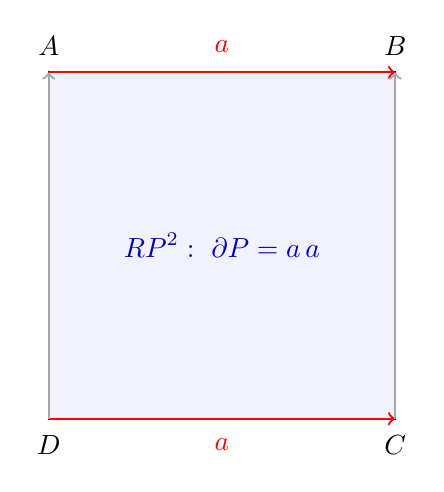
\begin{tikzpicture}[scale=2.2]
		% Square (fundamental polygon)
		\fill[blue!5] (-1,-1) rectangle (1,1);
		\draw[thick] (-1,-1) rectangle (1,1);
		
		% Label vertices (optional)
		\node[black] at (-1,1.15) {$A$};
		\node[black] at (1,1.15) {$B$};
		\node[black] at (1,-1.15) {$C$};
		\node[black] at (-1,-1.15) {$D$};
		
		% Top edge: a
		\draw[thick,red,->] (-1,1) -- (1,1);
		\node[red] at (0,1.15) {$a$};
		
		% Bottom edge: a (same orientation)
		\draw[thick,red,->] (-1,-1) -- (1,-1);
		\node[red] at (0,-1.15) {$a$};
		
		% Left/right edges (just gray guides)
		\draw[thick,gray!70,->] (-1,-1) -- (-1,1);
		\draw[thick,gray!70,->] (1,-1) -- (1,1);
		
		% Annotation
		\node[blue!80!black] at (0,0)
		{$\mathbb{RP}^2:\ \partial P = a\,a$};
		
	\end{tikzpicture}
	\caption{Fundamental polygon of $\mathbb{RP}^2$: a square with opposite edges identified in the same direction, giving the edge word $aa$.}
	\label{fig:RP2_fundamental_polygon}
\end{figure}

	
	\par\medskip\noindent\textbf{Sphere and Disk Models of $\mathbb{RP}^2$}\par\smallskip

	
	A natural question is:
	
	\begin{quote}
		The disk model is 2-dimensional, but the sphere model lives in $\mathbb{R}^3$.
		How can both represent the same space $\mathbb{RP}^2$?
	\end{quote}
	
	We explain this carefully and geometrically.
	
	\par\medskip\noindent\textbf{$\mathbb{RP}^2$ is a 2-dimensional manifold}\par\smallskip

	
	\begin{proposition}
		The real projective plane $\mathbb{RP}^2$ is a $2$-dimensional topological
		manifold.
	\end{proposition}
	
	\begin{proof}[Idea of proof]
		By definition
		\[
		\mathbb{RP}^2 = (\mathbb{R}^3 \setminus \{0\}) / \sim,
		\quad
		v \sim \lambda v \text{ for } \lambda \in \mathbb{R}\setminus\{0\},
		\]
		so each point of $\mathbb{RP}^2$ corresponds to a line through the origin in
		$\mathbb{R}^3$.  One can cover $\mathbb{RP}^2$ by affine charts of the form
		$\{[x:y:1]\}$, $\{[x:1:z]\}$, $\{[1:y:z]\}$, each homeomorphic to $\mathbb{R}^2$.
		These charts give it the structure of a $2$-dimensional manifold.
	\end{proof}
	
	Thus, any model of $\mathbb{RP}^2$ must be \emph{intrinsically} $2$-dimensional.
	
	\medskip
	
	The apparent discrepancy comes from the fact that one model is drawn in
	$\mathbb{R}^3$:
	
	\begin{itemize}
		\item The \emph{disk model} is manifestly 2-dimensional.
		\item The \emph{sphere model} uses a surface $S^2 \subset \mathbb{R}^3$, so we
		see it sitting in 3D, but the surface itself is 2-dimensional.
	\end{itemize}
	
	\par\medskip\noindent\textbf{Why does the sphere model start in $\mathbb{R}^3$?}\par\smallskip

	
	Consider the model
	\[
	\mathbb{RP}^2 \cong S^2 / (x \sim -x),
	\]
	where $S^2 \subset \mathbb{R}^3$ is the unit sphere and we identify antipodal points.
	
	\begin{itemize}
		\item The sphere $S^2$ is a $2$-dimensional surface embedded in $\mathbb{R}^3$.
		\item The ambient space $\mathbb{R}^3$ is irrelevant for the intrinsic
		dimension; we are only using the surface of the sphere.
		\item The quotient $S^2/(x\sim -x)$ still has topological dimension $2$,
		since identifying points in pairs does not increase dimension.
	\end{itemize}
	
	Hence:
	
	\begin{quote}
		The sphere model of $\mathbb{RP}^2$ is \emph{2-dimensional}, not 3-dimensional;
		it is only \emph{drawn} in 3D.
	\end{quote}
	
	This is analogous to a rubber sheet: it is 2-dimensional even if you place it
	in a 3-dimensional room.
	
	\par\medskip\noindent\textbf{The disk model as a fundamental domain}\par\smallskip

	
	The second standard model is
	\[
	\mathbb{RP}^2 \cong D^2 / (p \sim -p \text{ on } \partial D^2),
	\]
	where $D^2$ is the closed unit disk in $\mathbb{R}^2$ and points on the
	boundary circle are identified with their antipodes.
	
	Here:
	
	\begin{itemize}
		\item We start with a 2-dimensional disk $D^2$.
		\item We identify pairs of boundary points $p$ and $-p$.
		\item The resulting quotient is again a 2-dimensional surface.
	\end{itemize}
	
	This disk model is a \emph{fundamental domain} for the antipodal action on
	the sphere and is very convenient for:
	\begin{itemize}
		\item polygon gluings and classification of surfaces,
		\item describing the fundamental polygon,
		\item computing the fundamental group.
	\end{itemize}
	
	\par\medskip\noindent\textbf{Equivalence of the sphere and disk models}\par\smallskip

	
	We now explain explicitly how the sphere model and the disk model give the
	same space.
	
	\begin{definition}[Upper hemisphere]
		Let
		\[
		S^2 = \{(x,y,z)\in\mathbb{R}^3 : x^2 + y^2 + z^2 = 1\},
		\]
		and define the upper hemisphere
		\[
		H = \{(x,y,z)\in S^2 : z \ge 0\}.
		\]
	\end{definition}
	
	We look at equivalence classes
	\[
	[x,y,z] = \{(x,y,z),(-x,-y,-z)\}.
	\]
	
	\par\medskip\noindent\textbf{Step 1: From $S^2$ to the hemisphere.}\par\smallskip

	\begin{itemize}
		\item If $z>0$, then in the class $\{(x,y,z),(-x,-y,-z)\}$, exactly one
		representative has $z>0$, and the other has $z<0$.
		Thus, each such class meets $H$ in exactly one point.
		\item If $z=0$ (the equator), then the class
		$\{(x,y,0),(-x,-y,0)\}$ lies entirely in the equator, and the two points are antipodal.
	\end{itemize}
	
	Hence each equivalence class in $S^2/(x\sim -x)$ has
	\begin{itemize}
		\item exactly one representative in the \emph{interior} of $H$ ($z>0$), and
		\item either one or two representatives on the equator, which are then identified.
	\end{itemize}
	
	Morally, $\mathbb{RP}^2$ is ``the upper hemisphere with antipodal identification on the equator.''
	
	\par\medskip\noindent\textbf{Step 2: From hemisphere to disk.}\par\smallskip

	
	Define
	\[
	\pi : H \longrightarrow D^2, 
	\qquad
	\pi(x,y,z) = (x,y),
	\]
	where
	\[
	D^2 = \{(u,v)\in\mathbb{R}^2 : u^2 + v^2 \le 1\}.
	\]
	
	This map is a homeomorphism:
	
	\begin{itemize}
		\item On $H$, we have $x^2 + y^2 + z^2 = 1$ with $z \ge 0$, so
		$x^2 + y^2 \le 1$. Thus $(x,y)\in D^2$.
		\item Given $(u,v)\in D^2$, we can recover
		\[
		z = \sqrt{1 - u^2 - v^2},
		\]
		so the inverse is
		\[
		\pi^{-1}(u,v) = (u,v,\sqrt{1-u^2-v^2}).
		\]
	\end{itemize}
	
	Therefore the upper hemisphere $H$ is homeomorphic to the disk $D^2$
	via $(x,y,z)\mapsto(x,y)$.
	
	\par\medskip\noindent\textbf{Step 3: How the identification looks after flattening.}\par\smallskip

	
	Combining the steps:
	
	\begin{enumerate}
		\item We start with the quotient by the antipodal map:
		\[
		(x,y,z) \sim (-x,-y,-z).
		\]
		\item We choose representatives with $z\ge 0$ (i.e.\ in $H$).
		\item We project to the disk via $\pi(x,y,z) = (x,y)$.
	\end{enumerate}
	
	\emph{Interior points.}  
	If $z>0$, the class
	\[
	\{(x,y,z),(-x,-y,-z)\}
	\]
	has a unique representative in $H$, namely $(x,y,z)$, which maps to
	$(x,y)$ with $x^2 + y^2 < 1$. No further identification occurs there.
	Thus, points in the interior of $D^2$ are not glued to anything else.
	
	\medskip
	
	\emph{Boundary points (equator / circle).}  
	If $(x,y,0)$ lies on the equator, then
	\[
	(x,y,0) \mapsto (x,y), \qquad (-x,-y,0) \mapsto (-x,-y),
	\]
	both on the unit circle. In $\mathbb{RP}^2$, these two points are
	identified since they are antipodal.
	
	Therefore, in the disk picture:
	
	\begin{quote}
		On the boundary circle $\partial D^2$, each point $(u,v)$ is identified 
		with its opposite point $(-u,-v)$.
	\end{quote}
	
	This is precisely the disk model
	\[
	\mathbb{RP}^2 \cong D^2 / \bigl( (u,v)\sim(-u,-v) \text{ on } \partial D^2 \bigr).
	\]
	
	\par\medskip\noindent\textbf{Summary and comparison of the models}\par\smallskip

	
	We can summarize the relationship between the models in the following
	conceptual diagram:
	\[
	\begin{array}{ccc}
		S^2 & \xrightarrow{\ \text{quotient } x\sim -x\ } & \mathbb{RP}^2 \\[4pt]
		\Big\downarrow\text{restrict to } H & & \Big\uparrow\cong \\[4pt]
		H & \xrightarrow[\cong]{\ \pi\ } & D^2 / \bigl( p\sim -p \text{ on } \partial D^2 \bigr)
	\end{array}
	\]
	where $\pi(x,y,z) = (x,y)$.
	
	\begin{itemize}
		\item The \emph{sphere model} $S^2/(x\sim -x)$ emphasizes:
		\begin{itemize}
			\item compactness,
			\item non-orientability (the antipodal map reverses orientation),
			\item geometric and differential properties.
		\end{itemize}
		\item The \emph{disk model} $D^2/(p\sim -p)$ emphasizes:
		\begin{itemize}
			\item the fundamental polygon,
			\item the classification of surfaces,
			\item the edge word $aa$,
			\item computations of the fundamental group and other invariants.
		\end{itemize}
	\end{itemize}
	
	In both cases, the resulting space is a 2-dimensional manifold:
	
	\begin{quote}
		The dimension of $\mathbb{RP}^2$ is always $2$.  
		The sphere model uses a 2D surface embedded in $\mathbb{R}^3$; the ambient
		space plays no role in the intrinsic dimension.  
		The disk model works directly in $\mathbb{R}^2$.  
		The two models differ only in how we represent $\mathbb{RP}^2$, not in its
		dimension.
	\end{quote}
\end{solution}

\subsection*{Main-text correspondence: VII/02}

\begin{problem}[CP-VII-0005 --- Problem 1: Smoothly equivalent atlases and smooth functions]
\label{prob:cp-vii-0005}
Let $X$ be a topological $n$-manifold and let $\mathcal A,\mathcal B$ be smooth atlases on $X$.
\begin{enumerate}
	\item[(a)] Show that if $\mathcal A$ and $\mathcal B$ are smoothly equivalent, then they determine the same smooth functions:
	for any open $U\subset X$, a function $f:U\to\mathbb R$ is smooth w.r.t.\ $\mathcal A$ iff it is smooth w.r.t.\ $\mathcal B$.
	\item[(b)] Prove the converse. (Hint: consider local coordinate functions.)
\end{enumerate}

\medskip
\end{problem}

\begin{solution}
\smallskip
\noindent\textbf{(a)}
Assume $\mathcal A$ and $\mathcal B$ are smoothly equivalent, i.e.\ every chart in $\mathcal A$ is smoothly compatible
with every chart in $\mathcal B$.

Let $U\subset X$ be open and let $f:U\to\mathbb R$ be $\mathcal A$-smooth.
Pick any chart $(S,\psi)\in\mathcal B$. We must show $f\circ\psi^{-1}$ is smooth on $\psi(U\cap S)$.
Fix $p\in U\cap S$ and choose $(V,\varphi)\in\mathcal A$ with $p\in V$.
On the overlap $U\cap S\cap V$ we have the factorization
\[
f\circ\psi^{-1}
=
(f\circ\varphi^{-1})\circ(\varphi\circ\psi^{-1}).
\]
Here $f\circ\varphi^{-1}$ is smooth by $\mathcal A$-smoothness, and $\varphi\circ\psi^{-1}$ is smooth
because $\mathcal A$ and $\mathcal B$ are compatible. Hence $f\circ\psi^{-1}$ is smooth near $\psi(p)$,
and therefore smooth on $\psi(U\cap S)$. Thus $f$ is $\mathcal B$-smooth.
The reverse implication is symmetric, so $\mathcal A$-smooth $\Leftrightarrow$ $\mathcal B$-smooth.

\smallskip
\noindent\textbf{(b)}
Assume conversely that for every open $U\subset X$, a function $f:U\to\mathbb R$ is $\mathcal A$-smooth iff it is $\mathcal B$-smooth.
Take charts $(U,\varphi)\in\mathcal A$ and $(S,\psi)\in\mathcal B$ with $U\cap S\neq\varnothing$.
We prove the transition map $\varphi\circ\psi^{-1}:\psi(U\cap S)\to\varphi(U\cap S)$ is smooth (and similarly for its inverse).

Write $\varphi=(\varphi^1,\dots,\varphi^n)$ where $\varphi^i:U\to\mathbb R$ are the coordinate functions.
Each $\varphi^i$ is $\mathcal A$-smooth on $U$ (in $\varphi$-coordinates it is just a projection map),
hence by hypothesis each $\varphi^i$ is also $\mathcal B$-smooth on $U\cap S$.
Therefore each component $\varphi^i\circ\psi^{-1}$ is smooth on $\psi(U\cap S)$.
But
\[
\varphi\circ\psi^{-1}=(\varphi^1\circ\psi^{-1},\dots,\varphi^n\circ\psi^{-1}),
\]
so $\varphi\circ\psi^{-1}$ is smooth. The same argument using the coordinate functions of $\psi$
shows $\psi\circ\varphi^{-1}$ is smooth. Hence $\mathcal A$ and $\mathcal B$ are smoothly compatible,
i.e.\ smoothly equivalent.

\medskip
\noindent\textbf{Examples.}
\begin{itemize}
	\item On $X=\mathbb R^n$, the standard atlas and the atlas of all restrictions of standard charts to open sets are smoothly equivalent,
	so they define the same smooth functions.
	\item If $\mathcal A$ is any smooth atlas, its maximal atlas (all charts smoothly compatible with $\mathcal A$)
	is smoothly equivalent to $\mathcal A$ and produces exactly the same smooth functions.
\end{itemize}


\begin{figure}[htbp]
	\centering
	\begin{tikzpicture}[>=Latex, node distance=26mm and 26mm]
		\tikzset{
			box/.style={rounded corners=6pt, draw=black, thick, fill=gray!5, inner sep=7pt, align=center},
			arr/.style={->, thick},
		}
		\node[box] (X) {$U\cap S\cap V \subset X$};
		\node[box, right=of X] (R) {$\mathbb{R}^n$\\$\varphi$-coords};
		\node[box, below=of R] (R2) {$\mathbb{R}^n$\\$\psi$-coords};
		\node[box, right=of R] (reals) {$\mathbb{R}$};
		
		\draw[arr] (X) -- node[above] {$\varphi$} (R);
		\draw[arr] (X) -- node[left] {$\psi$} (R2);
		\draw[arr] (R) -- node[above] {$f\circ\varphi^{-1}$} (reals);
		\draw[arr] (R2) -- node[below] {$f\circ\psi^{-1}$} (reals);
		\draw[arr] (R2) -- node[right] {$\varphi\circ\psi^{-1}$} (R);
		
		\node[align=left] at ($(X)+(0,-2.0)$) {\small On overlaps:\quad $f\circ\psi^{-1}=(f\circ\varphi^{-1})\circ(\varphi\circ\psi^{-1})$.};
	\end{tikzpicture}
	\caption{Smooth compatibility transfers smoothness of $f$ between atlases.}
\end{figure}


% ---------- Figure 2 (improved): Converse via coordinate functions ----------
\begin{figure}[htbp]
	\centering
	
	\begin{tikzpicture}[>=Latex, line cap=round, line join=round,
		node distance=22mm and 28mm]
		
		% Colors
		\definecolor{PhiBlue}{RGB}{36,99,181}
		\definecolor{PsiGreen}{RGB}{34,139,34}
		\definecolor{TransRed}{RGB}{176,54,54}
		\definecolor{BoxFill}{RGB}{248,248,248}
		
		% Styles (fixed widths!)
		\tikzset{
			box/.style={
				rounded corners=8pt, draw=black, thick, fill=BoxFill,
				inner sep=7pt, align=center, minimum height=12mm
			},
			wide/.style={box, minimum width=34mm},
			mid/.style={box, minimum width=30mm},
			small/.style={box, minimum width=14mm},
			arrPhi/.style={->, thick, draw=PhiBlue},
			arrPsi/.style={->, thick, draw=PsiGreen},
			arrTrans/.style={->, thick, draw=TransRed},
			lbl/.style={font=\small}
		}
		
		% Nodes
		\node[mid] (X) {$U\cap S\subset X$};
		
		\node[wide, right=of X] (RnPhi)
		{$\mathbb R^n$\\[-1mm]\textcolor{PhiBlue}{\small $\varphi$-coords}};
		
		\node[wide, below=16mm of RnPhi] (RnPsi)
		{$\mathbb R^n$\\[-1mm]\textcolor{PsiGreen}{\small $\psi$-coords}};
		
		\node[small, right=22mm of RnPhi] (R) {$\mathbb R$};
		
		% Arrows (NO arrow crosses text)
		\draw[arrPhi] (X) -- node[above, lbl] {$\varphi$} (RnPhi);
		\draw[arrPsi] (X) -- node[sloped, below, lbl] {$\psi$} (RnPsi);
		
		\draw[arrTrans] (RnPsi) -- node[right, lbl] {$\varphi\circ\psi^{-1}$} (RnPhi);
		
		\draw[arrPhi] (RnPhi) to[bend left=12] node[above, lbl] {$\pi_i$} (R);
		\node[lbl, above=1mm of R] {\textcolor{PhiBlue}{$\varphi^i=\pi_i\circ\varphi$}};
		
	\end{tikzpicture}
	
	\caption{Converse: coordinate functions force transition smoothness.}
	
	\vspace{0.5em}
	\noindent\textbf{Key idea (with dimensions).}
	The charts have types $\varphi:U\to\mathbb R^n$ and $\psi:S\to\mathbb R^n$, hence
	$\varphi\circ\psi^{-1}:\psi(U\cap S)\to\varphi(U\cap S)\subset\mathbb R^n$.
	Writing $\varphi=(\varphi^1,\dots,\varphi^n)$ with $\varphi^i:U\to\mathbb R$, we have
	$\varphi^i\circ\psi^{-1}:\psi(U\cap S)\to\mathbb R$.
	A map into $\mathbb R^n$ is smooth iff all its components are smooth, so smoothness of every
	$\varphi^i\circ\psi^{-1}$ implies smoothness of $\varphi\circ\psi^{-1}$.
\end{figure}

\noindent\textbf{Figure explanation.}
Assume the class of $\mathcal A$-smooth real-valued functions equals the class of $\mathcal B$-smooth ones on every open set.
For a chart $(U,\varphi)\in\mathcal A$, each coordinate function $\varphi^i:U\to\mathbb R$ is $\mathcal A$-smooth, hence also $\mathcal B$-smooth.
Therefore $\varphi^i\circ\psi^{-1}$ is smooth on $\psi(U\cap S)$ for every overlapping $(S,\psi)\in\mathcal B$.
Since $\varphi\circ\psi^{-1}=(\varphi^1\circ\psi^{-1},\dots,\varphi^n\circ\psi^{-1})$, the transition map is smooth.


\begin{figure}[htbp]
	\centering
	\begin{tikzpicture}[>=Latex]
		\tikzset{
			box/.style={rounded corners=6pt, draw=black, thick, fill=gray!5, inner sep=8pt, align=center},
			arr/.style={->, thick},
		}
		\node[box] (eq) {Atlases $\mathcal A,\mathcal B$\\ are smoothly equivalent};
		\node[box, right=40mm of eq] (sf) {They define the same\\ smooth functions on all open sets};
		\node[box, below=14mm of sf] (trans) {All transition maps\\ $\varphi\circ\psi^{-1}$ are smooth};
		
		\draw[arr] (eq) -- node[above] {(a)} (sf);
		\draw[arr] (sf) -- node[right] {(b)} (trans);
		\draw[arr] (trans) -- node[left] {definition} (eq);
		
	\end{tikzpicture}
	\caption{Logic of Problem 1: equivalence of atlases is the same as agreeing on smooth functions.}
\end{figure}




% Theory: Problem 1


\par\medskip\noindent\textbf{Theory for Problem 1 (Atlases, smooth equivalence, smooth functions)}\par\smallskip


\par\medskip\noindent\textbf{Charts and atlases.}\par\smallskip

A \emph{chart} on a topological $n$-manifold $X$ is a homeomorphism
\[
\varphi:U\longrightarrow V\subset \mathbb R^n
\]
where $U\subset X$ is open and $V\subset\mathbb R^n$ is open.
An \emph{atlas} $\mathcal A$ is a collection of charts whose domains cover $X$.

\par\medskip\noindent\textbf{Smooth compatibility and smooth atlases.}\par\smallskip

Two charts $(U,\varphi)$ and $(S,\psi)$ are \emph{smoothly compatible} if the transition maps
\[
\varphi\circ \psi^{-1}:\psi(U\cap S)\to \varphi(U\cap S),
\qquad
\psi\circ \varphi^{-1}:\varphi(U\cap S)\to \psi(U\cap S)
\]
are $C^\infty$ maps between open subsets of $\mathbb R^n$.
An atlas is a \emph{smooth atlas} if every pair of its charts is smoothly compatible.

\par\medskip\noindent\textbf{Smooth equivalence of atlases.}\par\smallskip

Two smooth atlases $\mathcal A$ and $\mathcal B$ are \emph{smoothly equivalent} if every chart in $\mathcal A$
is smoothly compatible with every chart in $\mathcal B$.
Equivalently, $\mathcal A\cup\mathcal B$ is again a smooth atlas.

\par\medskip\noindent\textbf{Smooth functions defined by an atlas.}\par\smallskip

Given an atlas $\mathcal A$, a function $f:U\to\mathbb R$ (with $U\subset X$ open) is \emph{$\mathcal A$-smooth}
if for every chart $(V,\varphi)\in\mathcal A$ the coordinate expression
\[
f\circ \varphi^{-1}:\varphi(U\cap V)\to \mathbb R
\]
is smooth in the usual Euclidean sense.

\par\medskip\noindent\textbf{Componentwise smoothness.}\par\smallskip

A map $g=(g^1,\dots,g^n):W\subset\mathbb R^m\to\mathbb R^n$ is smooth if and only if each component
$g^i:W\to\mathbb R$ is smooth. This is the basic tool used to recover smoothness of a transition map from smoothness of
its coordinate components.

\par\medskip\noindent\textbf{Coordinate functions.}\par\smallskip

If $\varphi:U\to\mathbb R^n$ is a chart, write $\varphi=(\varphi^1,\dots,\varphi^n)$ with
coordinate functions $\varphi^i:U\to\mathbb R$.
In $\varphi$-coordinates, $\varphi^i$ becomes the standard projection $\pi_i:\mathbb R^n\to\mathbb R$,
so each $\varphi^i$ is automatically smooth with respect to any atlas containing $\varphi$.





% Problem 2
\end{solution}

\begin{problem}[CP-VII-0006 --- Problem 2: Homogeneous coordinate charts on $\mathbb{RP}^n$ and $\mathbb{CP}^n$]
\label{prob:cp-vii-0006}

\noindent\textbf{Problem statement.}
Show that the homogeneous coordinate maps on $\mathbb{RP}^n$ and $\mathbb{CP}^n$ define smooth pseudo-atlases.
Show that the resulting spaces are Hausdorff and second-countable, hence are smooth manifolds.

\medskip
\end{problem}

\begin{solution}
\smallskip
\noindent\textbf{(A) $\mathbb{RP}^n$.}
Recall $\mathbb{RP}^n$ consists of lines through $0$ in $\mathbb R^{n+1}$; write points as
$[x_0:\cdots:x_n]$ with $(x_0,\dots,x_n)\neq 0$ and $[x]=[\lambda x]$ for $\lambda\neq 0$.
For $i=0,\dots,n$ define
\[
U_i=\{[x_0:\cdots:x_n]\in\mathbb{RP}^n:\ x_i\neq 0\}.
\]
Define $\phi_i:U_i\to\mathbb R^n$ by
\[
\phi_i([x_0:\cdots:x_n])
=
\Big(\frac{x_0}{x_i},\dots,\frac{x_{i-1}}{x_i},\frac{x_{i+1}}{x_i},\dots,\frac{x_n}{x_i}\Big).
\]
This is well-defined since scaling cancels in the ratios. It is a bijection onto $\mathbb R^n$ with inverse
sending $y\in\mathbb R^n$ to the class with $i$-th coordinate $1$ and the remaining coordinates given by $y$.

On overlaps $U_i\cap U_j$, the transition maps $\phi_j\circ\phi_i^{-1}$ are given by rational expressions
(with denominators nonzero exactly on the overlap), hence are smooth. Therefore the homogeneous charts define a smooth atlas.

\smallskip
\noindent\textbf{(B) $\mathbb{CP}^n$.}
Similarly, points are complex lines in $\mathbb C^{n+1}$, written $[z_0:\cdots:z_n]$ with $[z]=[\lambda z]$, $\lambda\in\mathbb C^\times$.
Let
\[
V_i=\{[z_0:\cdots:z_n]\in\mathbb{CP}^n:\ z_i\neq 0\},
\qquad
\Phi_i:V_i\to\mathbb C^n
\]
be defined by
\[
\Phi_i([z_0:\cdots:z_n])
=
\Big(\frac{z_0}{z_i},\dots,\frac{z_{i-1}}{z_i},\frac{z_{i+1}}{z_i},\dots,\frac{z_n}{z_i}\Big).
\]
Transition maps are again rational in the complex coordinates, hence holomorphic on overlaps and therefore smooth
when we identify $\mathbb C^n\cong\mathbb R^{2n}$. Thus $\mathbb{CP}^n$ becomes a smooth manifold of real dimension $2n$.

\smallskip
\noindent\textbf{(C) Hausdorff and second-countable.}
Give $\mathbb{RP}^n$ (resp.\ $\mathbb{CP}^n$) the topology for which each chart map is a homeomorphism onto an open subset of $\mathbb R^n$
(resp.\ $\mathbb R^{2n}$): a set $O$ is open iff $\phi_i(O\cap U_i)$ is open for all $i$ (resp.\ $\Phi_i(O\cap V_i)$).

\begin{itemize}
	\item \emph{Hausdorff:} if two points lie in a common chart domain, separate their images in $\mathbb R^n$ (or $\mathbb R^{2n}$) by disjoint open sets
	and pull back. If they do not lie in a common chart domain, one can still separate using chart domains and their complements.
	\item \emph{Second-countable:} $\mathbb R^n$ has a countable basis $\mathcal B$. Then
	$\{\phi_i^{-1}(B): B\in\mathcal B,\ i=0,\dots,n\}$ is a countable basis (finite index set $\times$ countable set is countable).
\end{itemize}
Hence $\mathbb{RP}^n$ is a smooth $n$-manifold and $\mathbb{CP}^n$ is a smooth $2n$-manifold.

\medskip
\noindent\textbf{Examples.}
\begin{itemize}
	\item $\mathbb{RP}^1$ is a smooth $1$-manifold (in fact diffeomorphic to $S^1$).
	\item $\mathbb{CP}^1$ is a smooth $2$-manifold (in fact diffeomorphic to $S^2$, the Riemann sphere).
	\item In $\mathbb{RP}^2$, the transition between $\phi_0$ and $\phi_1$ has the form $(u,v)\mapsto (1/u,\,v/u)$ on the domain $u\neq 0$,
	hence is smooth on its overlap domain.
\end{itemize}



% Problem 3
\end{solution}

\begin{problem}[CP-VII-0007 --- Problem 3: Local chart criterion for smoothness of a map]
\label{prob:cp-vii-0007}
Let $X,Y$ be smooth manifolds with atlases
\[
\{\varphi_\alpha:U_\alpha\to V_\alpha\}_{\alpha\in A},
\qquad
\{\psi_\beta:S_\beta\to T_\beta\}_{\beta\in B}.
\]
Show that a map $F:X\to Y$ is smooth if and only if there exists a cover $\{W_\gamma\}_{\gamma\in C}$ of $X$ and
for each $\gamma$ there exist $\alpha(\gamma)\in A$ and $\beta(\gamma)\in B$ such that:
\begin{enumerate}
	\item[(a)] $W_\gamma\subset U_{\alpha(\gamma)}$ and $F(W_\gamma)\subset S_{\beta(\gamma)}$,
	\item[(b)] $\varphi_{\alpha(\gamma)}(W_\gamma)$ is open in $V_{\alpha(\gamma)}$,
	\item[(c)] the map
	\[
	\psi_{\beta(\gamma)}\circ F\circ \big(\varphi_{\alpha(\gamma)}\vert_{W_\gamma}\big)^{-1}
	:\ \varphi_{\alpha(\gamma)}(W_\gamma)\longrightarrow T_{\beta(\gamma)}
	\]
	is smooth.
\end{enumerate}

\medskip
\end{problem}

\begin{solution}
\smallskip
\noindent\textbf{($\Rightarrow$)}
Assume $F$ is smooth. For each $x\in X$, by the definition of smoothness choose charts
$(U_\alpha,\varphi_\alpha)$ around $x$ and $(S_\beta,\psi_\beta)$ around $F(x)$ such that
$\psi_\beta\circ F\circ\varphi_\alpha^{-1}$ is smooth on a neighborhood of $\varphi_\alpha(x)$.
Shrink to an open neighborhood $W_x\subset U_\alpha$ with $x\in W_x$, $F(W_x)\subset S_\beta$,
and $\varphi_\alpha(W_x)$ open, so that
\[
\psi_\beta\circ F\circ(\varphi_\alpha\vert_{W_x})^{-1}
\]
is smooth on $\varphi_\alpha(W_x)$. The sets $\{W_x\}_{x\in X}$ form an open cover; relabel by $\gamma$.

\smallskip
\noindent\textbf{($\Leftarrow$)}
Conversely assume such a cover $\{W_\gamma\}$ exists with smooth coordinate expressions in the chosen charts.
To prove $F$ is smooth in the usual sense, let $x\in X$ and choose arbitrary charts $(U,\varphi)$ about $x$
and $(S,\psi)$ about $F(x)$. Pick $\gamma$ with $x\in W_\gamma$.
On $\varphi(W_\gamma\cap U)$ we can write
\[
\psi\circ F\circ\varphi^{-1}
=
(\psi\circ\psi_{\beta(\gamma)}^{-1})
\circ
(\psi_{\beta(\gamma)}\circ F\circ\varphi_{\alpha(\gamma)}^{-1})
\circ
(\varphi_{\alpha(\gamma)}\circ\varphi^{-1}).
\]
The middle map is smooth by assumption (on the appropriate domain),
and the left/right maps are transition maps between charts in $Y$ and $X$, hence smooth.
Therefore $\psi\circ F\circ\varphi^{-1}$ is smooth near $\varphi(x)$.
Since $x$ was arbitrary, $F$ is smooth.

\medskip
\noindent\textbf{Examples.}
\begin{itemize}
	\item \emph{Inclusion $S^n\hookrightarrow\mathbb R^{n+1}$.}
	Using stereographic charts on $S^n$ and the standard chart on $\mathbb R^{n+1}$,
	the coordinate expression of the inclusion is smooth on each chart domain; hence the inclusion is smooth.
	\item \emph{Projective map induced by a linear map.}
	If $A:\mathbb R^{n+1}\to\mathbb R^{n+1}$ is invertible, then $F([x])=[Ax]$ defines $F:\mathbb{RP}^n\to\mathbb{RP}^n$.
	In homogeneous charts $U_i$, the coordinate formulas are quotients of linear functions (rational with nonzero denominators on overlaps),
	hence smooth; the cover criterion applies.
	\item \emph{Stereographic projection.}
	The stereographic map $S^2\setminus\{N\}\to\mathbb R^2$ is smooth because its coordinate formula is smooth on its domain.
\end{itemize}


% Theory: Problem 2


\par\medskip\noindent\textbf{Theory for Problem 2 (Homogeneous coordinates and projective manifolds)}\par\smallskip


\par\medskip\noindent\textbf{Projective space as a quotient.}\par\smallskip

Real projective space is the quotient
\[
\mathbb{RP}^n = (\mathbb R^{n+1}\setminus\{0\})/\sim,
\qquad
x\sim \lambda x \ \ (\lambda\in\mathbb R^\times),
\]
and complex projective space is
\[
\mathbb{CP}^n = (\mathbb C^{n+1}\setminus\{0\})/\sim,
\qquad
z\sim \lambda z \ \ (\lambda\in\mathbb C^\times).
\]
Elements are written in \emph{homogeneous coordinates} as $[x_0:\cdots:x_n]$ or $[z_0:\cdots:z_n]$.

\par\medskip\noindent\textbf{Standard chart domains.}\par\smallskip

For each $i=0,\dots,n$ define
\[
U_i=\{[x]\in\mathbb{RP}^n: x_i\neq 0\},
\qquad
V_i=\{[z]\in\mathbb{CP}^n: z_i\neq 0\}.
\]
These sets cover $\mathbb{RP}^n$ and $\mathbb{CP}^n$, respectively.

\par\medskip\noindent\textbf{Homogeneous coordinate charts.}\par\smallskip

Define charts
\[
\phi_i:U_i\to\mathbb R^n,
\qquad
\phi_i([x_0:\cdots:x_n])=
\Big(\frac{x_0}{x_i},\dots,\widehat{\frac{x_i}{x_i}},\dots,\frac{x_n}{x_i}\Big),
\]
where the hat means the $i$-th slot is omitted.
Similarly,
\[
\Phi_i:V_i\to\mathbb C^n,
\qquad
\Phi_i([z_0:\cdots:z_n])=
\Big(\frac{z_0}{z_i},\dots,\widehat{\frac{z_i}{z_i}},\dots,\frac{z_n}{z_i}\Big).
\]
These maps are well-defined because scaling by $\lambda$ cancels in the ratios.

\par\medskip\noindent\textbf{Transition maps are rational.}\par\smallskip

On overlaps $U_i\cap U_j$, the transition functions $\phi_j\circ\phi_i^{-1}$ are given by rational expressions
whose denominators are nonzero on the overlap, hence are smooth.
On overlaps $V_i\cap V_j$, the transition functions $\Phi_j\circ\Phi_i^{-1}$ are holomorphic (rational),
and therefore smooth when we identify $\mathbb C^n\cong \mathbb R^{2n}$.

\par\medskip\noindent\textbf{Topology, Hausdorffness, and second-countability.}\par\smallskip

Declare $O\subset\mathbb{RP}^n$ open iff $\phi_i(O\cap U_i)$ is open in $\mathbb R^n$ for all $i$
(and similarly for $\mathbb{CP}^n$ using $\Phi_i$).
With this topology:
\begin{itemize}
	\item $\mathbb{RP}^n$ and $\mathbb{CP}^n$ are Hausdorff since points can be separated inside a common chart by disjoint Euclidean open sets.
	\item They are second-countable: if $\mathcal B$ is a countable basis of $\mathbb R^n$ (resp.\ $\mathbb R^{2n}$), then
	$\{\phi_i^{-1}(B):B\in\mathcal B,\ i=0,\dots,n\}$ (resp.\ $\{\Phi_i^{-1}(B)\}$) is a countable basis.
\end{itemize}
Hence the homogeneous coordinate pseudo-atlases define smooth manifolds with
\[
\dim(\mathbb{RP}^n)=n,
\qquad
\dim_{\mathbb R}(\mathbb{CP}^n)=2n.
\]


% Problem 3
\end{solution}

\begin{problem}[CP-VII-0008 --- Problem 10 (Boundary of a manifold; the square has corners)]
\label{prob:cp-vii-0008}
\textbf{(i) Statement.} Prove that the boundary $\partial X$ of a smooth $n$-manifold with boundary $X$
is a smooth $(n-1)$-manifold without boundary.

\medskip
\end{problem}

\begin{solution}
By definition, for each $p\in X$ there exists a smooth chart $(U,\varphi)$ with
\[
\varphi:U\stackrel{\cong}{\longrightarrow} V\subset \mathbb{H}^n,
\qquad \mathbb{H}^n=\{u\in\mathbb{R}^n:\ u_n\ge 0\},
\]
such that coordinate changes are smooth up to the boundary.

A point $p\in X$ lies in $\partial X$ iff in some (hence any) boundary chart one has
$\varphi(p)\in \partial\mathbb{H}^n=\{u_n=0\}$.

Fix $p\in \partial X$ and choose a boundary chart $(U,\varphi)$ around $p$ with
$\varphi(U)=V\subset \mathbb{H}^n$. Let $\pi:\mathbb{R}^n\to\mathbb{R}^{n-1}$ be the projection
$\pi(u_1,\dots,u_n)=(u_1,\dots,u_{n-1})$ and define
\[
\psi := \pi\circ \varphi \;:\; U\cap \partial X \longrightarrow \pi(V\cap \{u_n=0\}) \subset \mathbb{R}^{n-1}.
\]
Then $\psi$ is a homeomorphism onto an open subset of $\mathbb{R}^{n-1}$ because
$V\cap\{u_n=0\}$ is open in $\{u_n=0\}\cong \mathbb{R}^{n-1}$ and $\varphi$ is a homeomorphism.
If $(U,\varphi)$ and $(U',\varphi')$ are two boundary charts, the transition map on $\partial X$ is
\[
\psi'\circ \psi^{-1}
= (\pi\circ \varphi')\circ (\pi\circ \varphi)^{-1},
\]
which is the restriction (to $u_n=0$) of the smooth map $\varphi'\circ \varphi^{-1}$ between open subsets of
$\mathbb{H}^n$, hence is smooth as a map between open subsets of $\mathbb{R}^{n-1}$.
Therefore these charts form a smooth atlas on $\partial X$, modeled on $\mathbb{R}^{n-1}$,
so $\partial X$ is a smooth $(n-1)$-manifold \emph{without} boundary.

\bigskip
\textbf{(ii) Statement.} Show that the square $[0,1]\times[0,1]\subset \mathbb{R}^2$ is not a smooth manifold with boundary
(as a smooth submanifold-with-boundary of $\mathbb{R}^2$).

\medskip
\noindent\textbf{Solution.}
Assume for contradiction that $M:=[0,1]\times[0,1]$ were a smooth $2$-dimensional submanifold with boundary of $\mathbb{R}^2$.
Then by part (i), $\partial M$ would be a smooth $1$-dimensional submanifold of $\mathbb{R}^2$ (a smooth embedded curve),
so for every $p\in \partial M$ there exists a neighborhood $W\subset \mathbb{R}^2$ of $p$ and a smooth diffeomorphism
$\Phi:W\to \Phi(W)\subset \mathbb{R}^2$ such that
\[
\Phi(M\cap W) = \mathbb{H}^2\cap \Phi(W), \qquad
\Phi(\partial M\cap W)=\{(x,0)\}\cap \Phi(W).
\]
In particular, $\partial M\cap W$ must be the inverse image of a straight line segment under a diffeomorphism,
hence must be a smooth embedded $1$-manifold near $p$ with a \emph{unique} tangent direction at $p$.

Take the corner point $p=(0,0)$. For every sufficiently small neighborhood $W$ of $p$,
the set $\partial M\cap W$ is the union of two line segments:
\[
(\{0\}\times[0,\varepsilon)) \;\cup\; ([0,\varepsilon)\times\{0\}),
\]
meeting at a right angle at $p$. This set does not have a unique tangent line at $p$ (it has two distinct tangent directions),
so it cannot be a smooth embedded $1$-submanifold near $p$. Contradiction.

Hence $[0,1]\times[0,1]$ is not a smooth manifold with boundary (it is a manifold with corners).




\par\medskip\noindent\textbf{Extra theory for Problem 10 (Boundary of a manifold; corners)}\par\smallskip


\noindent\textbf{Manifolds with boundary.}
A (smooth) $n$-manifold with boundary is a Hausdorff, second countable space $X$
equipped with an atlas of charts
\[
(U,\varphi),\qquad \varphi:U\stackrel{\cong}{\longrightarrow} V\subset \mathbb{H}^n,
\quad
\mathbb{H}^n=\{u\in\mathbb{R}^n:\ u_n\ge 0\},
\]
such that all transition maps are smooth (and extend smoothly across $u_n=0$ in local coordinates).

\medskip
\noindent\textbf{Interior and boundary (intrinsic definition).}
A point $p\in X$ is an \emph{interior point} if in some (equivalently any) boundary chart
$\varphi(p)$ lies in the interior of $\mathbb{H}^n$, i.e. $(\varphi(p))_n>0$.
A point $p\in X$ is a \emph{boundary point} if in some chart $\varphi(p)$ lies on
\[
\partial\mathbb{H}^n=\{u\in\mathbb{R}^n:\ u_n=0\}.
\]
The set of boundary points is denoted $\partial X$, and the interior is denoted $\mathrm{int}(X)$.
One has $X=\mathrm{int}(X)\,\dot\cup\,\partial X$.

\medskip
\noindent\textbf{Local model for the boundary.}
In a boundary chart $(U,\varphi)$ with $\varphi(U)=V\subset\mathbb{H}^n$, the boundary part is
\[
U\cap\partial X \;\cong\; V\cap\{u_n=0\},
\]
which is open in the hyperplane $\{u_n=0\}\cong\mathbb{R}^{n-1}$.
Projecting away the last coordinate
\[
\pi(u_1,\dots,u_n)=(u_1,\dots,u_{n-1})
\]
produces a coordinate chart for $\partial X$ modeled on $\mathbb{R}^{n-1}$.
This is the basic reason why $\partial X$ is an $(n-1)$-manifold without boundary.

\medskip
\noindent\textbf{What fails for the square: corners.}
The subset $[0,1]^2\subset\mathbb{R}^2$ has points (the four vertices) where a neighborhood in the set
looks like a \emph{quadrant}
\[
\mathbb{R}^2_{\ge 0,\ge 0}=\{(u_1,u_2): u_1\ge 0,\ u_2\ge 0\},
\]
not like a half-plane $\mathbb{H}^2=\{u_2\ge 0\}$.
At such a corner point, the boundary is locally the union of two smooth arcs meeting with a nonzero angle,
so it is not a smooth $1$-submanifold (there is no unique tangent direction).
Therefore the square is not a smooth manifold with boundary; it is an example of a \emph{manifold with corners}.

\medskip
\noindent\textbf{Remark (manifolds with corners).}
One can enlarge the definition by allowing local models
\[
[0,\infty)^k\times \mathbb{R}^{n-k},
\]
which yields the notion of a smooth manifold with corners.
Then the square $[0,1]^2$ is a $2$-manifold with corners (with $k=2$ at the vertices).


\par\medskip\noindent\textbf{Examples for Problem 10 (manifolds with boundary vs corners)}\par\smallskip


\noindent\textbf{Examples of manifolds with boundary.}
\begin{itemize}
	\item $[0,1]\subset\mathbb{R}$ is a $1$-manifold with boundary and $\partial[0,1]=\{0,1\}$.
	\item The closed disk $D^2=\{(x,y)\in\mathbb{R}^2:\ x^2+y^2\le 1\}$ is a $2$-manifold with boundary
	and $\partial D^2=S^1$.
	\item More generally, the closed ball $D^n=\{x\in\mathbb{R}^n:\ \|x\|\le 1\}$ is an $n$-manifold with boundary
	and $\partial D^n=S^{n-1}$.
	\item The cylinder $S^1\times[0,1]$ is a $2$-manifold with boundary and
	\[
	\partial(S^1\times[0,1])=(S^1\times\{0\})\sqcup(S^1\times\{1\}).
	\]
	\item The M\"obius strip is a $2$-manifold with boundary; its boundary is a single circle.
\end{itemize}

\noindent\textbf{Examples of manifolds without boundary.}
\begin{itemize}
	\item $S^n$ and $T^n$ are compact manifolds without boundary.
	\item The open ball $\{x\in\mathbb{R}^n:\ \|x\|<1\}$ is a manifold without boundary (modeled on $\mathbb{R}^n$).
\end{itemize}

\medskip
\noindent\textbf{Corner nonexample.}
The square $[0,1]^2$ fails to be a smooth manifold with boundary because neighborhoods of corner points
look like the quadrant $[0,\infty)^2$, not like the half-space $\mathbb{H}^2$.
Equivalently, near a corner the boundary is the union of two line segments meeting at a nonzero angle,
so it does not have a unique tangent direction.



\par\medskip\noindent\textbf{Definition of the boundary and why $\dim(\partial X)=n-1$}\par\smallskip


\noindent\textbf{Definition (manifold with boundary).}
A smooth $n$-manifold with boundary is a Hausdorff, second countable space $X$ equipped with an atlas of charts
\[
(U,\varphi),\qquad \varphi:U\stackrel{\cong}{\longrightarrow} V\subset \mathbb{H}^n,
\qquad
\mathbb{H}^n=\{u\in\mathbb{R}^n:\ u_n\ge 0\},
\]
such that all transition maps are smooth (and extend smoothly up to $u_n=0$).

\medskip
\noindent\textbf{Definition (interior and boundary).}
A point $p\in X$ is an \emph{interior point} if for some (equivalently any) chart $(U,\varphi)$ around $p$ one has
$(\varphi(p))_n>0$.
A point $p\in X$ is a \emph{boundary point} if for some (equivalently any) chart $(U,\varphi)$ around $p$ one has
$(\varphi(p))_n=0$.
The set of boundary points is denoted
\[
\partial X := \{p\in X:\ (\varphi(p))_n=0 \text{ in boundary coordinates}\},
\]
and the set of interior points is denoted $\mathrm{int}(X)=X\setminus\partial X$.

\medskip
\noindent\textbf{Why this is well-defined.}
If $(U,\varphi)$ and $(U',\varphi')$ are boundary charts, then the transition map
$\varphi'\circ\varphi^{-1}$ is a diffeomorphism between open subsets of $\mathbb{H}^n$.
Such maps preserve the boundary hyperplane $\partial\mathbb{H}^n=\{u_n=0\}$, hence the condition
$(\varphi(p))_n=0$ does not depend on the choice of boundary chart.

\medskip
\noindent\textbf{Why $\dim(\partial X)=n-1$.}
Near a boundary point $p\in\partial X$, choose a boundary chart $(U,\varphi)$ with $\varphi(U)=V\subset\mathbb{H}^n$.
Then
\[
U\cap \partial X \;\cong\; V\cap \{u_n=0\},
\]
and $V\cap\{u_n=0\}$ is open in the hyperplane $\{u_n=0\}\cong \mathbb{R}^{n-1}$.
Thus $\partial X$ is locally modeled on $\mathbb{R}^{n-1}$, so it is an $(n-1)$-dimensional manifold (without boundary).

\par\medskip\noindent\textbf{Charts around a point; diffeomorphisms in the definition; counterexamples (Problem 10)}\par\smallskip


\noindent\textbf{Local charts (interior vs boundary).}
Let $X$ be a smooth $n$-manifold with boundary.

\begin{itemize}
	\item If $p\in \mathrm{int}(X)$, then there is a chart $(U,\varphi)$ with
	\[
	\varphi:U\to V\subset \mathbb{R}^n,
	\]
	so $X$ looks locally like an open subset of $\mathbb{R}^n$ (a full ball).
	
	\item If $p\in \partial X$, then there is a chart $(U,\varphi)$ with
	\[
	\varphi:U\to V\subset \mathbb{H}^n=\{u\in\mathbb{R}^n:\ u_n\ge 0\},
	\]
	so $X$ looks locally like a half-ball. Moreover $U\cap\partial X$ corresponds to $V\cap\{u_n=0\}$.
\end{itemize}

\medskip
\noindent\textbf{How diffeomorphisms enter (flattening the boundary).}
In the embedded setting (a submanifold-with-boundary of $\mathbb{R}^m$), the definition is often phrased as:
for each $p\in X\subset\mathbb{R}^m$ there is a neighborhood $W$ of $p$ in $\mathbb{R}^m$ and a diffeomorphism
$\Phi:W\to \Phi(W)\subset\mathbb{R}^m$ such that
\[
\Phi(X\cap W)=\bigl(\mathbb{H}^n\times\{0\}\bigr)\cap \Phi(W),
\qquad
\Phi(\partial X\cap W)=\bigl(\{u_n=0\}\times\{0\}\bigr)\cap \Phi(W).
\]
Thus, near boundary points, a diffeomorphism straightens the boundary to a coordinate hyperplane.

\medskip
\noindent\textbf{Explicit flattening example (unit disk).}
Let $D^2=\{(x,y)\in\mathbb{R}^2:\ x^2+y^2\le 1\}$ and $p=(1,0)\in\partial D^2$.
Near $p$ the boundary circle is given by the smooth graph
\[
x=\sqrt{1-y^2}\qquad (y\text{ near }0).
\]
Define local coordinates $(u,w)$ by
\[
u=y,\qquad w=\sqrt{1-u^2}-x.
\]
Then $\partial D^2$ corresponds to $w=0$ and $D^2$ corresponds to $w\ge 0$.
Moreover the Jacobian at $p$ is invertible:
\[
\frac{\partial(u,w)}{\partial(x,y)}\Big|_{(1,0)}
=
\begin{pmatrix}
	0 & 1\\
	-1 & 0
\end{pmatrix},
\qquad \det=1\neq 0,
\]
so this is a local diffeomorphism straightening the boundary to the half-space $w\ge 0$.

\medskip
\noindent\textbf{Counterexamples (why corners/cusps fail).}
\begin{itemize}
	\item The square $[0,1]^2$ is not a smooth manifold with boundary: at a corner, neighborhoods look like a quadrant
	$[0,\infty)^2$, not like the half-space $\mathbb{H}^2$; equivalently the boundary has two tangent directions.
	\item More generally, any region with a corner (two smooth boundary arcs meeting at a nonzero angle) fails to be a manifold with boundary.
	\item If the boundary has a cusp (not a smooth embedded $(n-1)$-submanifold), then boundary charts with smooth transitions cannot exist.
\end{itemize}

\medskip
\noindent\textbf{Figures.}

\begin{figure}[htbp]
	\centering
	\begin{minipage}{0.40\linewidth}
		\centering
		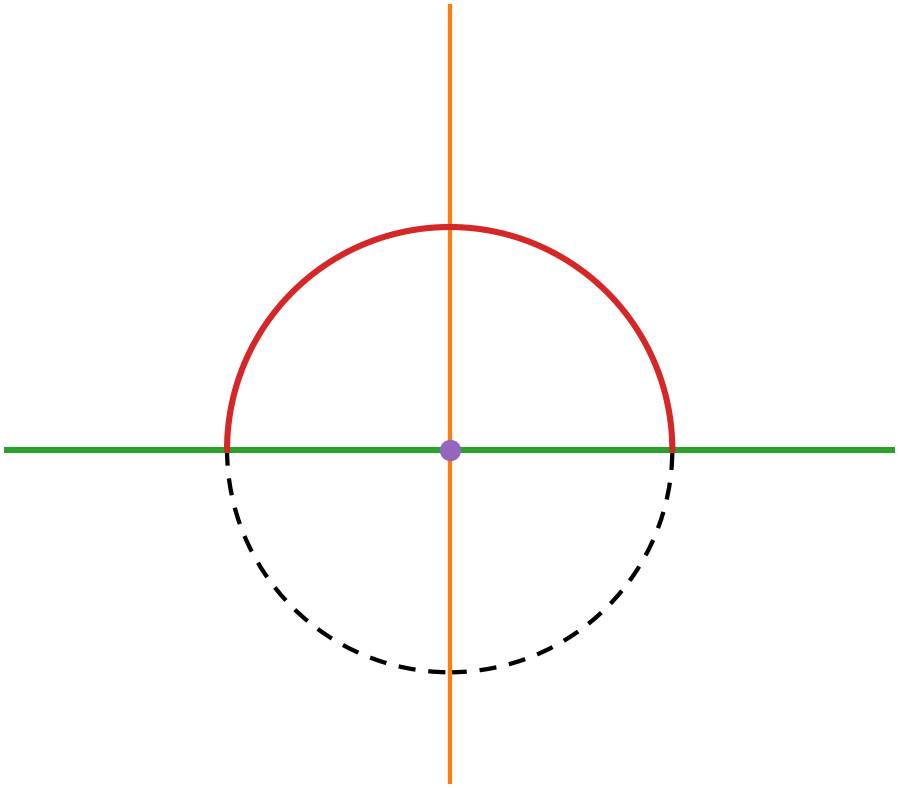
\includegraphics[width=\linewidth]{chapters/part07_volume_vii/figures/fig10_halfplane_model.png}
		\caption*{(a) Local model $\mathbb{H}^2$ with boundary $y=0$.}
	\end{minipage}\hfill
	\begin{minipage}{0.40\linewidth}
		\centering
		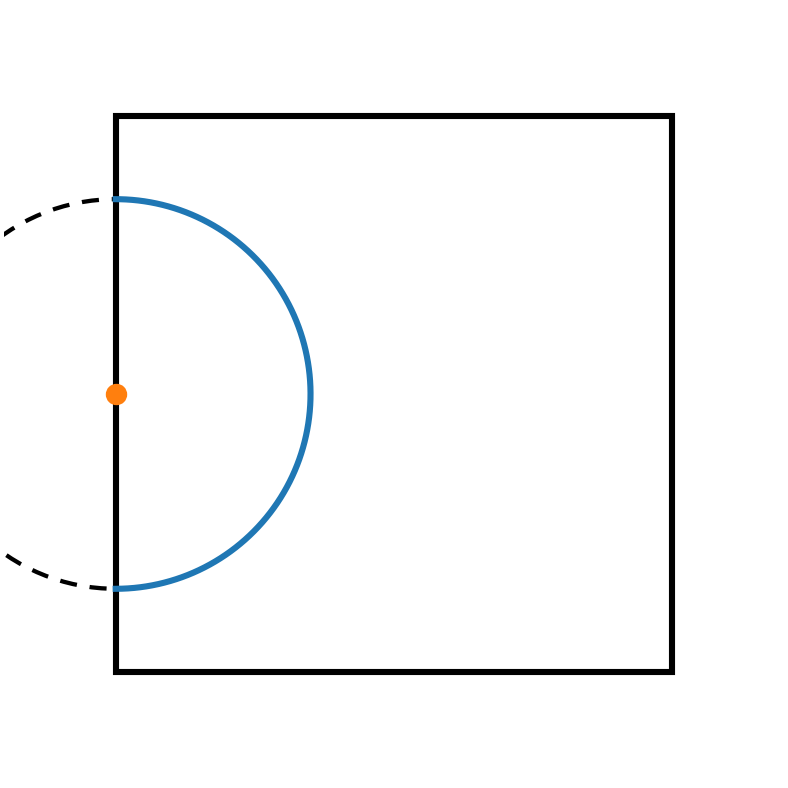
\includegraphics[width=\linewidth]{chapters/part07_volume_vii/figures/fig10_square_edge_neighborhood.png}
		\caption*{(b) Square: edge point has half-disk neighborhood.}
	\end{minipage}
	
	\medskip
	
	\begin{minipage}{0.40\linewidth}
		\centering
		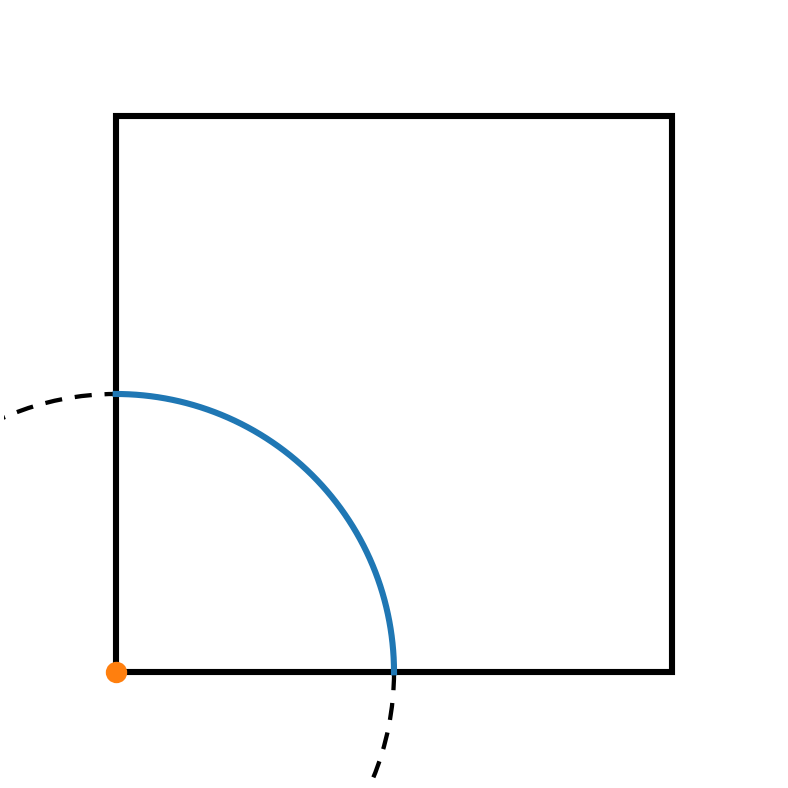
\includegraphics[width=\linewidth]{chapters/part07_volume_vii/figures/fig10_square_corner_neighborhood.png}
		\caption*{(c) Square: corner point has quarter-disk neighborhood.}
	\end{minipage}\hfill
	\begin{minipage}{0.40\linewidth}
		\centering
		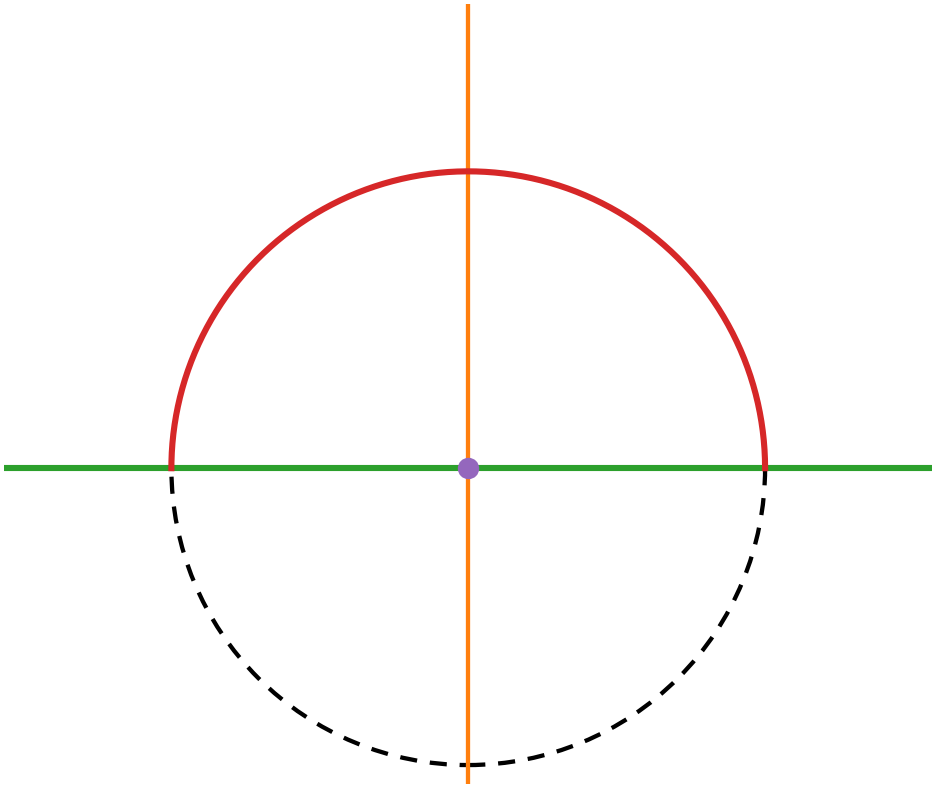
\includegraphics[width=\linewidth]{chapters/part07_volume_vii/figures/fig10_flattened_boundary_halfspace.png}
		\caption*{(d) Flattened boundary coordinates: $w\ge 0$, boundary $w=0$.}
	\end{minipage}
	
	\medskip
	
	\begin{minipage}{0.40\linewidth}
		\centering
		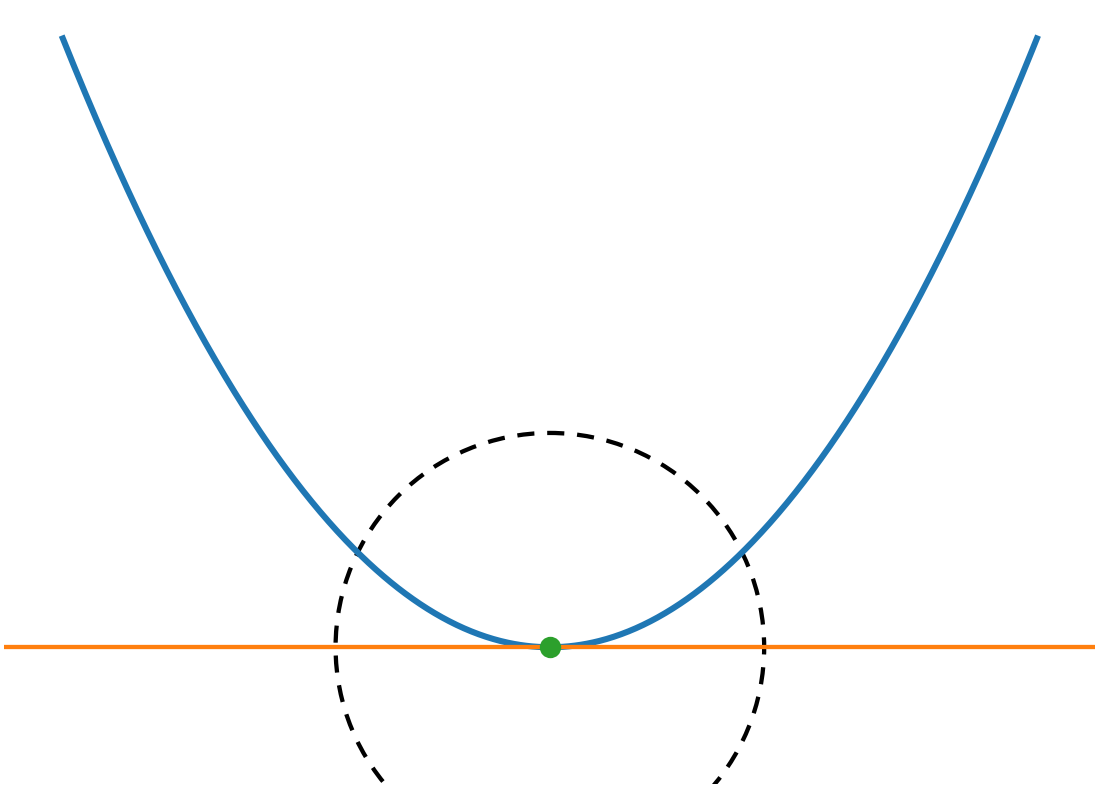
\includegraphics[width=\linewidth]{chapters/part07_volume_vii/figures/fig10_smooth_boundary_graph_neighborhood.png}
		\caption*{(e) Smooth boundary: $y=x^2$ (tangent exists).}
	\end{minipage}\hfill
	\begin{minipage}{0.40\linewidth}
		\centering
		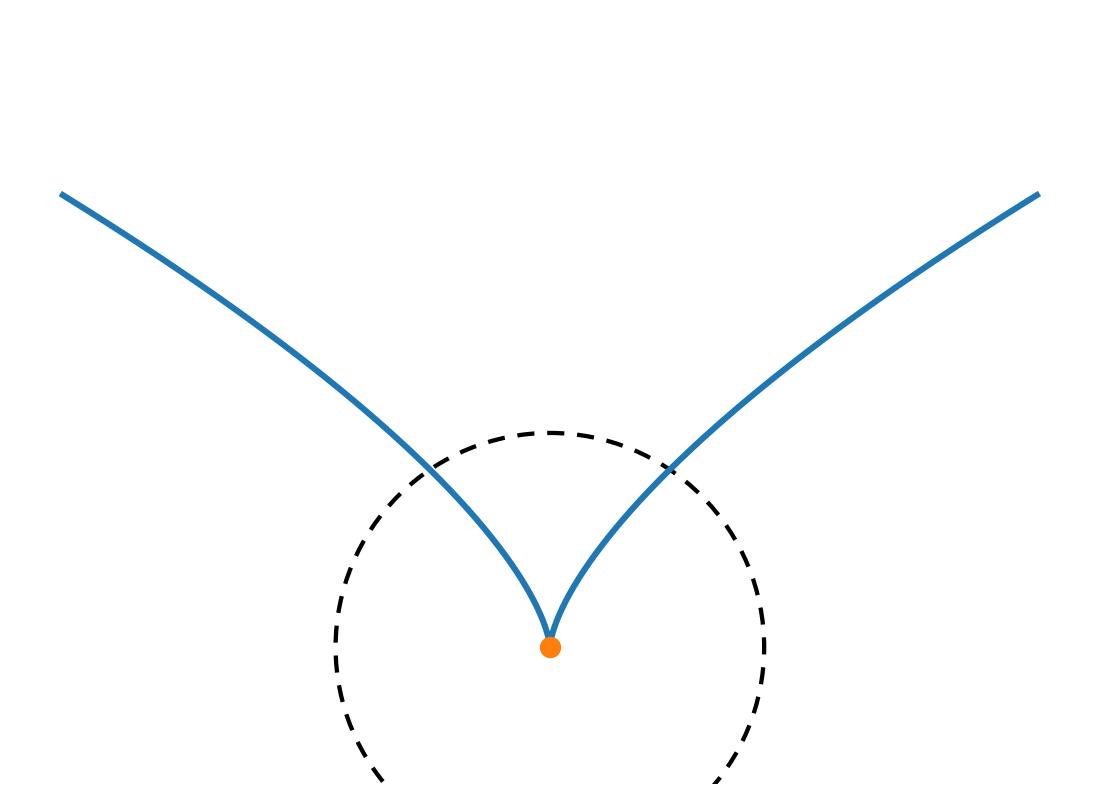
\includegraphics[width=\linewidth]{chapters/part07_volume_vii/figures/fig10_cusp_boundary_neighborhood.png}
		\caption*{(f) Cusp boundary: $y=|x|^{2/3}$ (not smooth at $0$).}
	\end{minipage}
	
	\caption{Neighborhood models: boundary charts look like half-spaces; corners and cusps fail.}
\end{figure}



\par\medskip\noindent\textbf{Lemma: transition maps preserve the boundary (used in Problem 10)}\par\smallskip


\noindent\textbf{Lemma.}
Let $U,V\subset \mathbb{H}^n$ be open and let $\psi:U\to V$ be a diffeomorphism such that $\psi$ and $\psi^{-1}$
extend smoothly to diffeomorphisms between open subsets of $\mathbb{R}^n$.
Then
\[
\psi\bigl(U\cap \partial\mathbb{H}^n\bigr)=V\cap \partial\mathbb{H}^n,
\qquad
\psi\bigl(U\cap \mathrm{int}(\mathbb{H}^n)\bigr)=V\cap \mathrm{int}(\mathbb{H}^n).
\]

\medskip
\noindent\textbf{Proof.}
Write $\partial\mathbb{H}^n=\{u_n=0\}$ and $\mathrm{int}(\mathbb{H}^n)=\{u_n>0\}$.
It suffices to show that $\psi$ cannot send a boundary point to an interior point.

Assume for contradiction that $x\in U$ satisfies $x_n=0$ but $y:=\psi(x)$ satisfies $y_n>0$.
Since $y$ is an interior point of $\mathbb{H}^n$ and $V$ is open in $\mathbb{H}^n$, there exists a small Euclidean ball
$B\subset \mathbb{R}^n$ such that
\[
y\in B \subset V \subset \mathbb{H}^n
\quad\text{and}\quad
B\subset\{u_n>0\}.
\]
Let $\widetilde\psi$ be a smooth extension of $\psi$ to an open neighborhood $W\subset\mathbb{R}^n$ of $x$,
so that $\widetilde\psi:W\to \widetilde\psi(W)$ is a diffeomorphism and $\widetilde\psi|_U=\psi$.
Then $\widetilde\psi^{-1}(B)$ is an open neighborhood of $x$ in $\mathbb{R}^n$.
In particular, it contains points with negative last coordinate, so we can choose $x'\in \widetilde\psi^{-1}(B)$ with $x'_n<0$.
Set $y':=\widetilde\psi(x')\in B$.

But $B\subset V\subset\mathbb{H}^n$, hence $y'\in V$ and $\psi^{-1}(y')$ is defined and must lie in $U\subset\mathbb{H}^n$,
so its last coordinate is $\ge 0$. On the other hand,
\[
\psi^{-1}(y')=\widetilde\psi^{-1}(y')=x',
\]
which has $x'_n<0$. Contradiction.

Therefore boundary points map to boundary points, and interior points map to interior points, proving the claim.
\qed

\begin{figure}[htbp]
	\centering
	
	\begin{minipage}{0.48\linewidth}
		\centering
		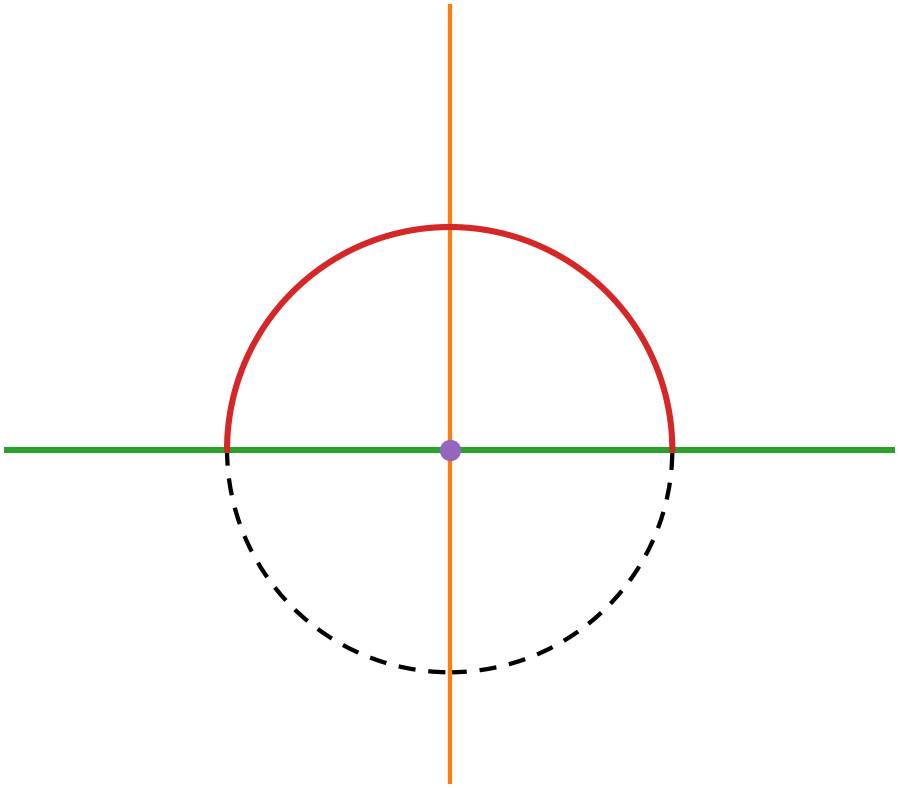
\includegraphics[width=\linewidth]{chapters/part07_volume_vii/figures/fig10_halfplane_model.png}
		\caption*{(a) Model $\mathbb{H}^2$ and boundary.}
	\end{minipage}\hfill
	\begin{minipage}{0.48\linewidth}
		\centering
		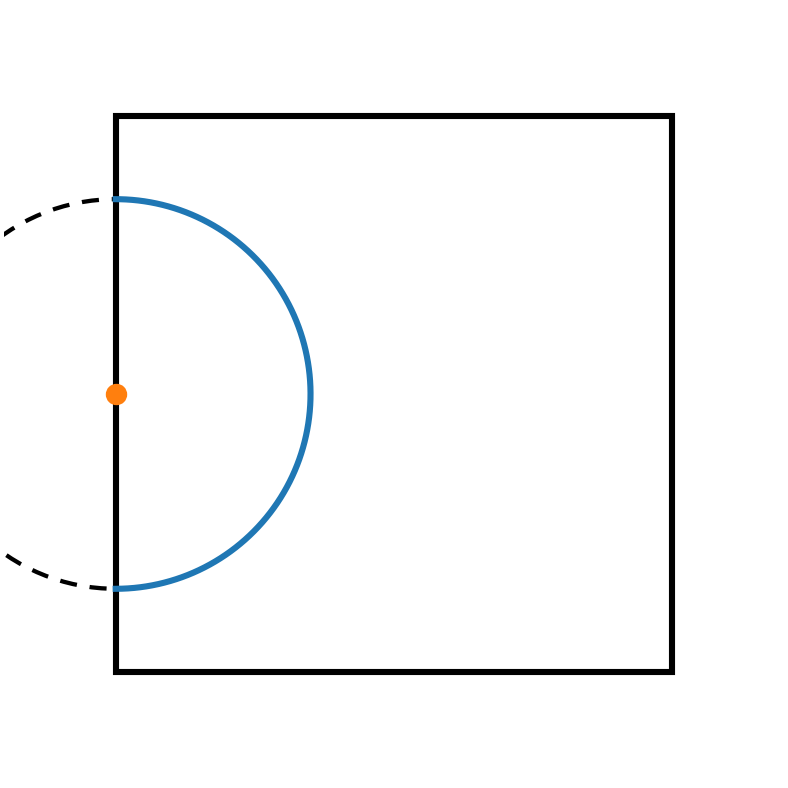
\includegraphics[width=\linewidth]{chapters/part07_volume_vii/figures/fig10_square_edge_neighborhood.png}
		\caption*{(b) Edge point: half-disk neighborhood.}
	\end{minipage}
	
	\medskip
	
	\begin{minipage}{0.48\linewidth}
		\centering
		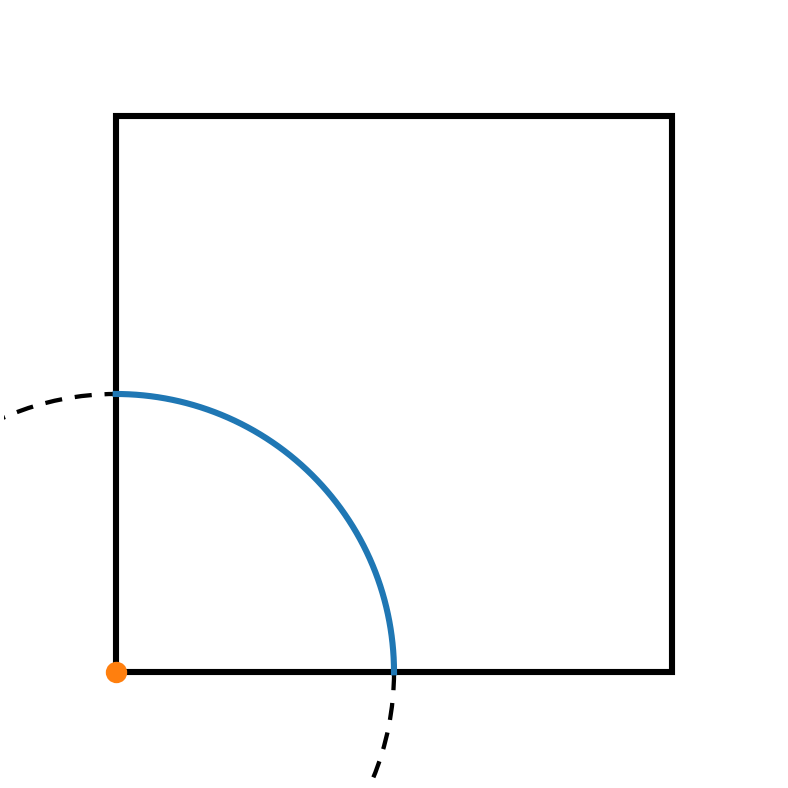
\includegraphics[width=\linewidth]{chapters/part07_volume_vii/figures/fig10_square_corner_neighborhood.png}
		\caption*{(c) Corner point: quarter-disk neighborhood.}
	\end{minipage}\hfill
	\begin{minipage}{0.48\linewidth}
		\centering
		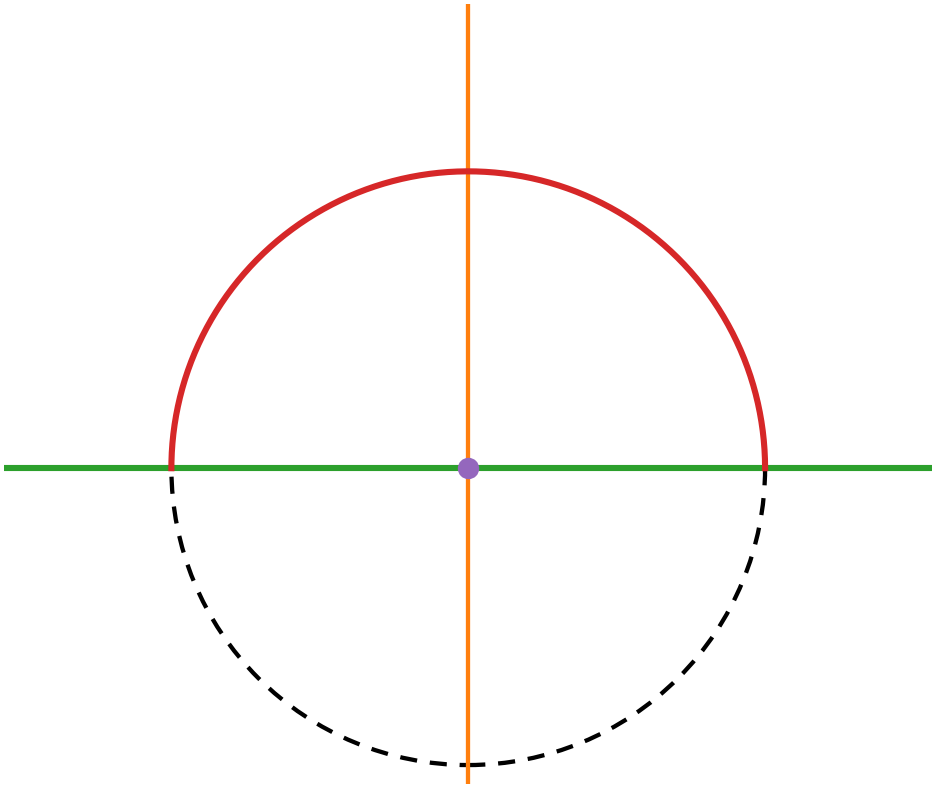
\includegraphics[width=\linewidth]{chapters/part07_volume_vii/figures/fig10_flattened_boundary_halfspace.png}
		\caption*{(d) Flattened coordinates: $w\ge 0$, boundary $w=0$.}
	\end{minipage}
	
	\caption{Neighborhoods in the local models: boundary charts look like half-spaces; corners do not.}
\end{figure}
\end{solution}

\begin{problem}[CP-VII-0009 --- Problem 5]
\label{prob:cp-vii-0009}
\end{problem}

\begin{solution}
\begin{enumerate}[label=\textnormal{(\alph*)}]
\item
For $(x,y,z)\in S^2$ with $z\neq 1$ the stereographic projection from the north
		pole is
		\[
		\pi_+(x,y,z) = \left(\frac{x}{1-z}, \frac{y}{1-z}\right),
		\]
		and from the south pole
		\[
		\pi_-(x,y,z) = \left(\frac{x}{1+z}, \frac{y}{1+z}\right),
		\]
		both with inverses defined on $\mathbb{R}^2$.
		For $(u,v)\in\mathbb{R}^2$ write $r^2 = u^2+v^2$.  Then
		\[
		\pi_+^{-1}(u,v)
		= \left(
		\frac{2u}{1+r^2},
		\frac{2v}{1+r^2},
		\frac{r^2-1}{1+r^2}
		\right).
		\]
		Hence
		\[
		\pi_- \circ \pi_+^{-1}(u,v)
		= \left(
		\frac{\frac{2u}{1+r^2}}{1+\frac{r^2-1}{1+r^2}},
		\frac{\frac{2v}{1+r^2}}{1+\frac{r^2-1}{1+r^2}}
		\right)
		= \left(
		\frac{u}{r^2},
		\frac{v}{r^2}
		\right)
		= \left(
		\frac{u}{u^{2}+v^{2}},
		\frac{v}{u^{2}+v^{2}}
		\right)
		\]
		on $\mathbb{R}^2 \setminus \{0\}$.  This map and its inverse are smooth,
		so the two charts $\pi_+$ and $\pi_-$ are smoothly compatible, and they define
		an atlas giving $S^2$ the structure of an abstract smooth surface.
		
		\medskip
		
		\item
		Now consider the chart on $S^2$ given by $(U,\phi)$ where
		$U = \{ y < 0 \}$ and $\phi : U \to \mathbb{R}^2$ maps $(x,y,z) \mapsto (x,z)$.
		What is the image of $\phi$?
		Check explicitly that this chart is compatible with the smooth atlas defined
		by $\pi_{\pm}$, i.e.\ the transition functions for the atlas with charts
		$\{\pi_{+},\pi_{-},\phi\}$ are all smooth.
		
		\medskip
		\textbf{Solution.}
		If $(x,y,z)\in S^2$, then $x^2+y^2+z^2=1$.  On $U$ we have $y<0$, hence
		\[
		y = -\sqrt{1-x^2-z^2}
		\]
		and necessarily $x^2+z^2 < 1$.
		Conversely, for any $(u,v)\in\mathbb{R}^2$ with $u^2+v^2<1$ we can define
		\[
		\phi^{-1}(u,v) = \bigl(u,\,-\sqrt{1-u^2-v^2},\,v\bigr) \in U \subset S^2.
		\]
		Thus
		\[
		\phi(U) = \{(u,v)\in\mathbb{R}^2 : u^2+v^2<1\},
		\]
		the open unit disc.
		
		To check compatibility, consider, for instance,
		$\pi_+ \circ \phi^{-1} : \phi(U) \to \mathbb{R}^2$:
		for $(u,v)$ with $u^2+v^2<1$,
		\[
		\phi^{-1}(u,v) = (u,-\sqrt{1-u^2-v^2},v) = (x,y,z),
		\]
		so
		\[
		\pi_+(x,y,z)
		= \left(\frac{x}{1-z},\frac{y}{1-z}\right)
		= \left(
		\frac{u}{1-v},
		\frac{-\sqrt{1-u^2-v^2}}{1-v}
		\right).
		\]
		Here $1-v>0$ on the unit disc, and the right-hand side is clearly a smooth
		function of $(u,v)$.  Similarly
		\[
		\pi_-(x,y,z)
		= \left(
		\frac{u}{1+v},
		\frac{-\sqrt{1-u^2-v^2}}{1+v}
		\right)
		\]
		is smooth on the disc.  The maps $\phi \circ \pi_\pm^{-1}$ are compositions
		of these with the inverses $\pi_\pm^{-1}$, hence are smooth.
		Thus $\phi$ is smoothly compatible with $\pi_\pm$, and the atlas
		$\{\pi_+,\pi_-,\phi\}$ is a smooth atlas on $S^2$.
		
		\medskip
		
		\item
		Let $a : S^2 \to S^2$ denote the antipodal map, $x \mapsto -x$.
		Show that $a$ is a diffeomorphism of the abstract smooth surface $S^2$, and
		deduce that the real projective plane $\mathbb{R}P^{2}$ also admits the
		structure of an abstract smooth surface.
		
		\medskip
		\textbf{Solution.}
		The map $A:\mathbb{R}^3\to\mathbb{R}^3$, $A(x)=-x$, is linear and hence
		smooth, and it restricts to a map $a=S^2\to S^2$.  To see that $a$ is smooth
		as a map of the abstract smooth surface $S^2$, consider its local expression
		in the stereographic charts:
		\[
		\Phi_+ := \pi_+ \circ a \circ \pi_+^{-1} : \mathbb{R}^2 \to \mathbb{R}^2.
		\]
		Both $\pi_+^{-1}$ and $\pi_+$ are smooth, as is $a$ in $\mathbb{R}^3$, so
		$\Phi_+$ is smooth.  The same argument applies for $\pi_-$.  Since
		$a^{-1}=a$ has the same coordinate expressions, the inverse is also smooth.
		Thus $a$ is a diffeomorphism of $S^2$.
		
		Define an equivalence relation on $S^2$ by $x\sim -x$, and write
		$\mathbb{R}P^2 = S^2/\sim$ for the set of equivalence classes.
		The action of the group $\mathbb{Z}_2 = \{ \mathrm{id}, a\}$ on $S^2$ is
		smooth, free and properly discontinuous.  For any chart $(U,\varphi)$ on
		$S^2$ with $U\cap a(U)=\varnothing$, the projection
		$q:S^2\to\mathbb{R}P^2$ restricts to a homeomorphism of $U$ onto $q(U)$, and
		we can use $\varphi$ as a coordinate map on $q(U)$ via this identification.
		Transition maps between such charts on $\mathbb{R}P^2$ are induced by the
		transition maps on $S^2$, and hence are smooth.
		
		Therefore $\mathbb{R}P^2$ admits an atlas of compatible smooth charts and
		thus carries the structure of an abstract smooth surface.
	
	
	
	\begin{figure}[h]
		\centering
		\begin{tikzpicture}[scale=2, >=Stealth]
			
			% Plane z = 0 as a tilted rectangle
			\fill[gray!10]
			(-2,-0.3) -- (2,-0.3) -- (1.6,0.1) -- (-2,0.1) -- cycle;
			\draw
			(-2,-0.3) -- (2,-0.3) -- (1.6,0.1) -- (-2,0.1) -- cycle;
			\node at (-1.7,-0.1) {$z=0$};
			
			% Sphere
			\draw (0,0) circle (1);
			
			% Equator (ellipse: front solid, back dashed)
			\draw (-1,0) arc (180:0:1 and 0.35);           % front
			\draw[dashed] (-1,0) arc (180:360:1 and 0.35); % back
			
			% North pole N
			\coordinate (N) at (0,1);
			\fill (N) circle (0.02);
			\node[above] at (N) {$N$};
			
			% Point p on the upper hemisphere
			\coordinate (P) at (0.5,0.6);
			\fill (P) circle (0.02);
			\node[right] at (P) {$p$};
			
			% Image of p under stereographic projection from N
			% Direction from N to P is (0.5, -0.4); extend until y = -0.2
			% 1 + t*(-0.4) = -0.2  => t = 3, so point is (1.5, -0.2).
			\coordinate (Q) at (1.5,-0.2);
			\fill (Q) circle (0.02);
			\node[right] at (Q) {$\pi_+(p)$};
			
			% Line from N through p to the plane
			\draw (N) -- (P);
			\draw[->] (N) -- (Q);
			
		\end{tikzpicture}
		\caption{Stereographic projection $\pi_+$ from the north pole $N$ onto the plane $z=0$.}
		\label{fig:stereographic-tikz}
	\end{figure}
\end{enumerate}
\end{solution}

\subsection*{Main-text correspondence: VII/03}

\begin{problem}[CP-VII-0010 --- Problem 2: A diffeomorphism from a ball onto $\mathbb{R}^k$]
\label{prob:cp-vii-0010}
\par\medskip\noindent\textbf{Problem.}\par\smallskip

Let $B_r=\{x\in\mathbb{R}^k:\|x\|<r\}$ be the open ball. Show that the map
\[
F:B_r\longrightarrow \mathbb{R}^k,\qquad
F(x)=\frac{r\,x}{\sqrt{r^2-\|x\|^2}}
\]
is a diffeomorphism of $B_r$ onto $\mathbb{R}^k$.
\end{problem}

\begin{solution}
\textbf{(1) Smoothness of $F$.}
On $B_r$ we have $r^2-\|x\|^2>0$, hence $\sqrt{r^2-\|x\|^2}$ is a smooth function of $x$.
Thus $F$ is smooth on $B_r$.

\medskip
\textbf{(2) Construct the inverse map.}
Given $y=F(x)$, we compute
\[
\|y\|^2=\frac{r^2\|x\|^2}{r^2-\|x\|^2}.
\]
Solving for $\|x\|^2$ gives
\[
\|x\|^2=\frac{r^2\|y\|^2}{r^2+\|y\|^2}.
\]
Then
\[
r^2-\|x\|^2
=r^2-\frac{r^2\|y\|^2}{r^2+\|y\|^2}
=\frac{r^4}{r^2+\|y\|^2},
\qquad
\sqrt{r^2-\|x\|^2}=\frac{r^2}{\sqrt{r^2+\|y\|^2}}.
\]
From $y=\dfrac{r x}{\sqrt{r^2-\|x\|^2}}$ we obtain
\[
y= \frac{r x}{r^2/\sqrt{r^2+\|y\|^2}}
= x\cdot\frac{\sqrt{r^2+\|y\|^2}}{r}
\quad\Longrightarrow\quad
x=\frac{r\,y}{\sqrt{r^2+\|y\|^2}}.
\]
Define
\[
G:\mathbb{R}^k\to \mathbb{R}^k,\qquad
G(y)=\frac{r\,y}{\sqrt{r^2+\|y\|^2}}.
\]
We have $\|G(y)\|^2=\dfrac{r^2\|y\|^2}{r^2+\|y\|^2}<r^2$, so $G(y)\in B_r$ for all $y$.
Moreover, a direct substitution shows
\[
F(G(y))=y\quad(\forall y\in\mathbb{R}^k),
\qquad
G(F(x))=x\quad(\forall x\in B_r).
\]
Thus $G=F^{-1}$.

\medskip
\textbf{(3) Smoothness of the inverse.}
The map $G$ is smooth on all of $\mathbb{R}^k$ because $r^2+\|y\|^2>0$ everywhere.
Hence $F$ is bijective, smooth, and has a smooth inverse: $F$ is a diffeomorphism
$B_r\cong\mathbb{R}^k$.
\qed

\par\medskip\noindent\textbf{Remark.}\par\smallskip

If a chart maps a neighborhood in a manifold onto a ball $B_r\subset\mathbb{R}^k$,
then composing with the above diffeomorphism $B_r\to\mathbb{R}^k$ yields a chart
whose coordinate domain is all of $\mathbb{R}^k$.


\par\medskip\noindent\textbf{How this implies charts can be chosen with domain $\mathbb{R}^k$.}\par\smallskip

Let $M$ be a smooth $k$-manifold and let $(U,\varphi)$ be a chart, so
$\varphi:U\to \varphi(U)\subset\mathbb{R}^k$ is a diffeomorphism onto an open set.
Fix $p\in U$ and set $a=\varphi(p)$.

Since $\varphi(U)$ is open, there exists $r>0$ such that the Euclidean ball
$B_r(a)\subset \varphi(U)$. Let $T_{-a}(x)=x-a$ be translation by $-a$ and define
\[
\psi := T_{-a}\circ \varphi : U\longrightarrow \varphi(U)-a .
\]
Then $\psi$ is a diffeomorphism, $\psi(p)=0$, and $B_r(0)\subset \psi(U)$.

Now set
\[
U' := \psi^{-1}(B_r(0))\subset U.
\]
Then $\psi|_{U'}:U'\to B_r(0)$ is a diffeomorphism.

By Problem 2, the map
\[
F:B_r(0)\longrightarrow \mathbb{R}^k,\qquad
F(x)=\frac{r\,x}{\sqrt{r^2-\|x\|^2}}
\]
is a diffeomorphism. Therefore the composition
\[
\Phi := F\circ \psi|_{U'} : U'\longrightarrow \mathbb{R}^k
\]
is a diffeomorphism onto all of $\mathbb{R}^k$.
Hence, after possibly shrinking the neighborhood, one may always choose local
coordinates whose coordinate domain is the whole space $\mathbb{R}^k$.

\begin{figure}[htbp]
	\centering
	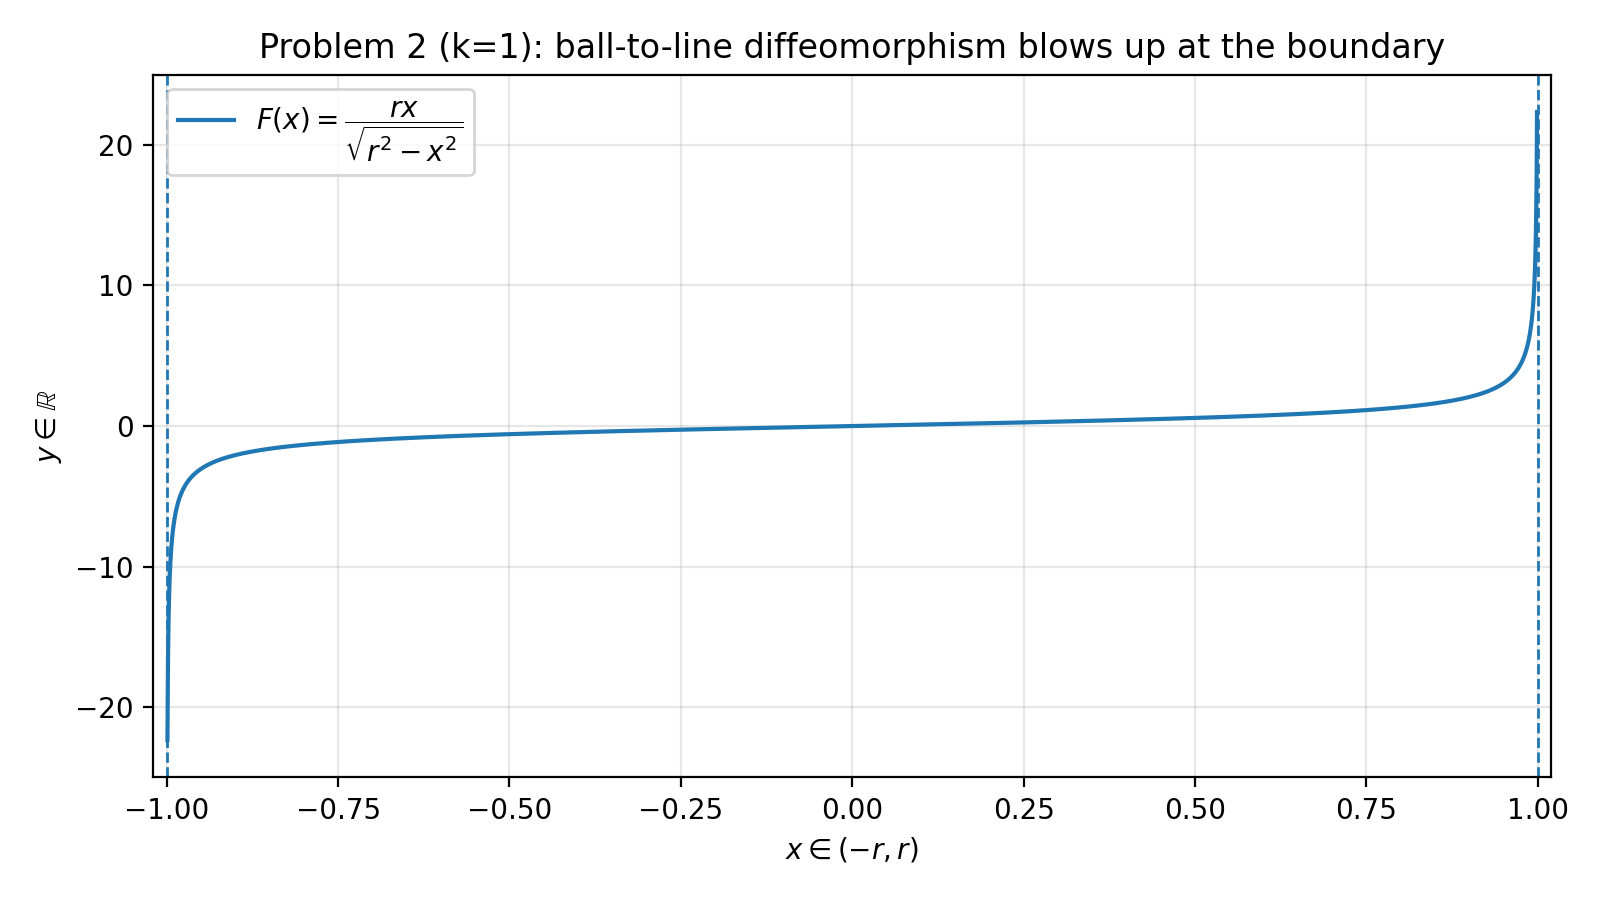
\includegraphics[width=0.85\textwidth]{chapters/part07_volume_vii/figures/problem2_map_1d.png}
	\caption{(Problem 2, $k=1$, $r=1$) The map $F(x)=\dfrac{rx}{\sqrt{r^2-x^2}}$ blows up as $x\to \pm r$, so the boundary of the interval is sent to infinity.}
\end{figure}

\begin{figure}[htbp]
	\centering
	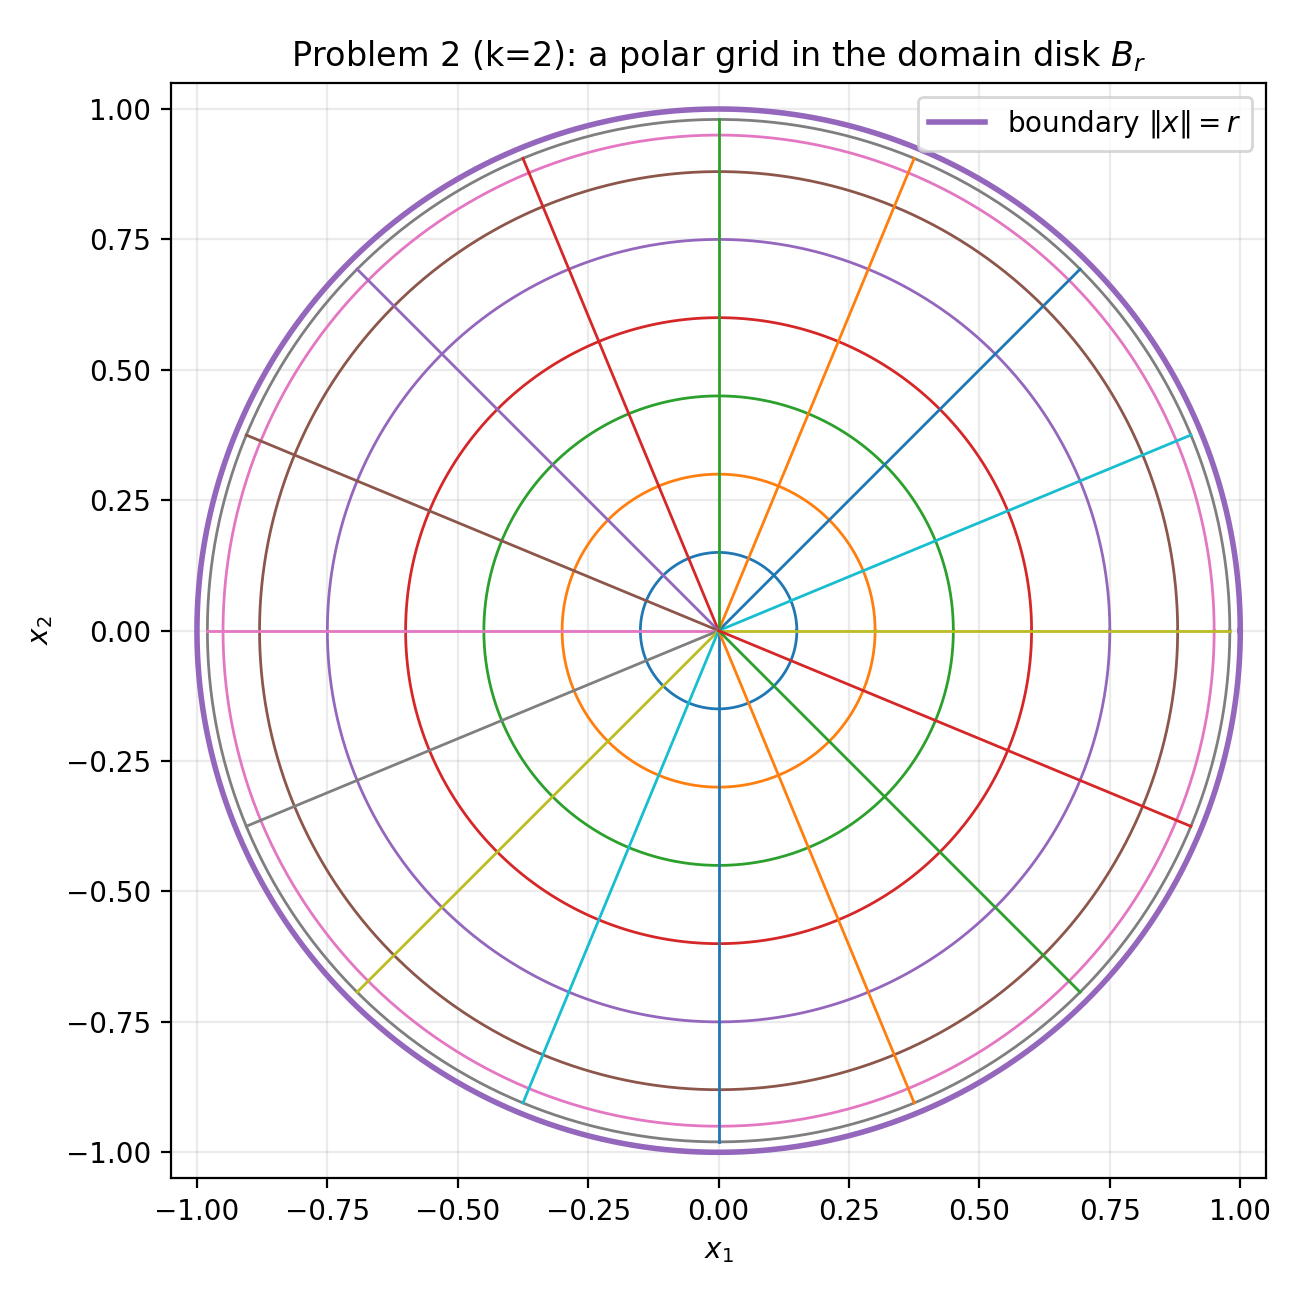
\includegraphics[width=0.62\textwidth]{chapters/part07_volume_vii/figures/problem2_disk_grid.png}
	\caption{(Problem 2, $k=2$, $r=1$) A polar grid in the domain disk $B_r$. Circles $\|x\|=\rho$ and rays $\theta=\mathrm{const}$ are shown.}
\end{figure}

\begin{figure}[htbp]
	\centering
	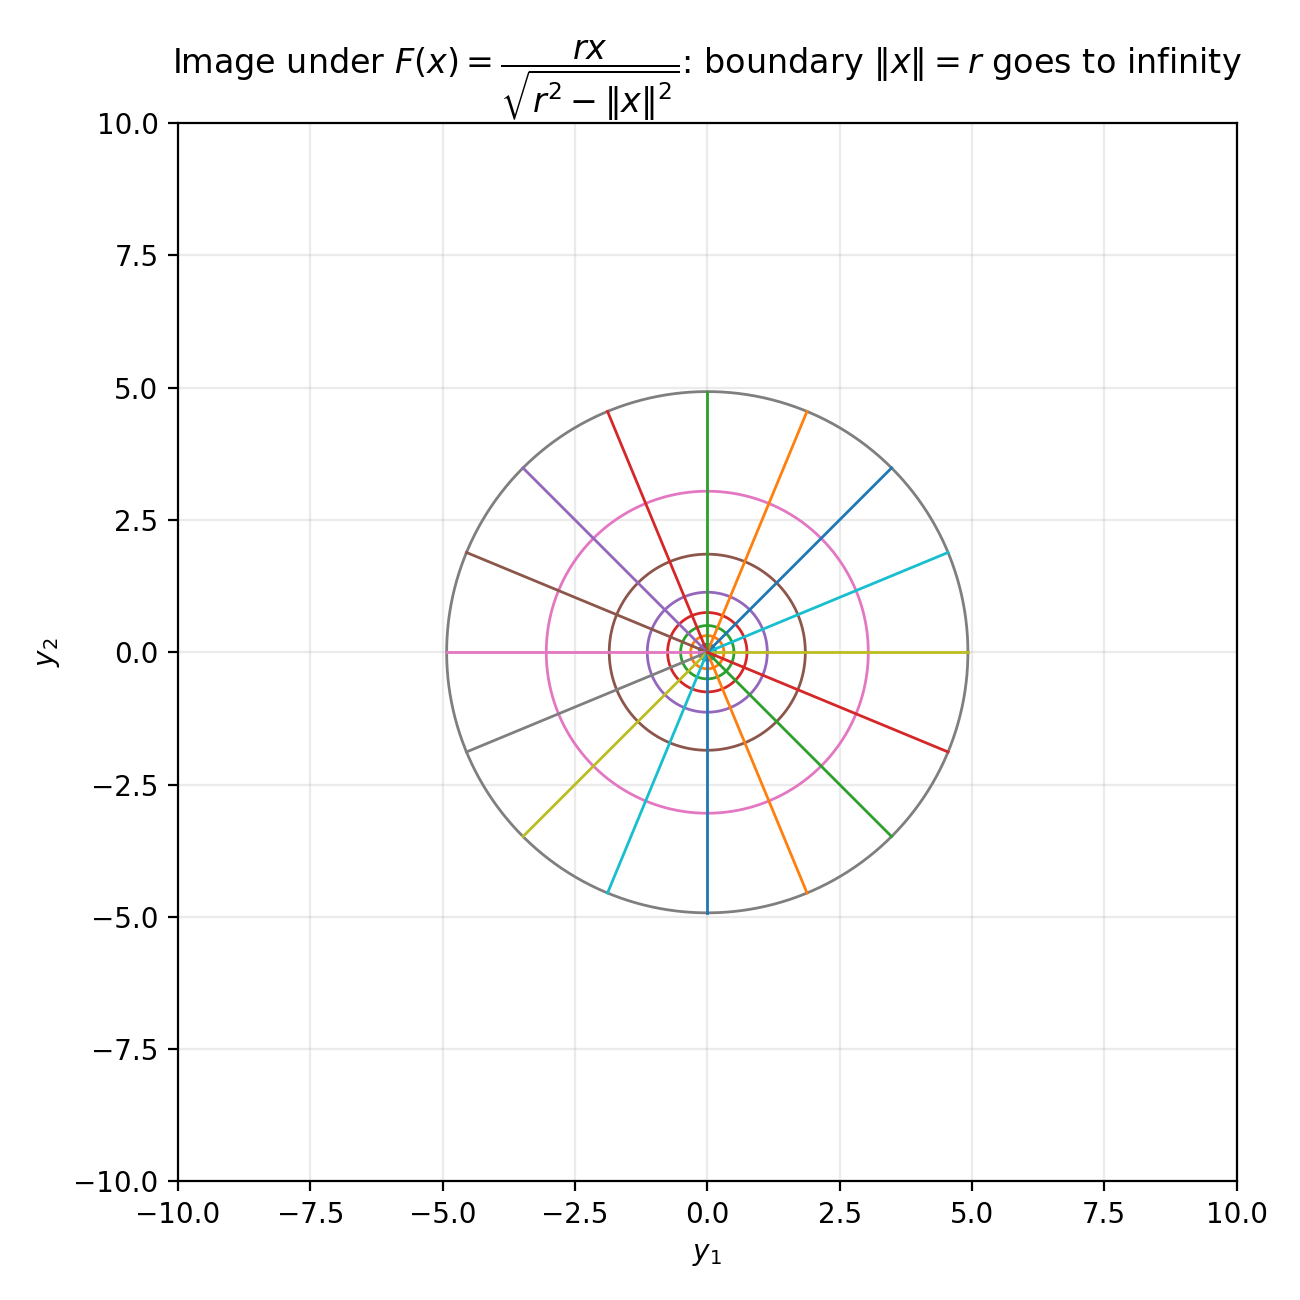
\includegraphics[width=0.62\textwidth]{chapters/part07_volume_vii/figures/problem2_image_grid.png}
	\caption{Image of the grid under $F(x)=\dfrac{r x}{\sqrt{r^2-\|x\|^2}}$. Rays stay rays and circles map to circles, while the boundary $\|x\|=r$ is pushed out to infinity.}
\end{figure}


\clearpage

% ------------------------------------------------------------
\end{solution}

\begin{problem}[CP-VII-0011 --- Problem 9 (Lefschetz map on a compact manifold has finitely many fixed points)]
\label{prob:cp-vii-0011}
Let $f:X\to X$ be smooth. Assume that for every fixed point $x$ of $f$,
the linear map $Df_x:T_xX\to T_xX$ does not have $1$ as an eigenvalue.
Prove: if $X$ is compact and $f$ is Lefschetz, then $f$ has only finitely many fixed points.

\medskip
\end{problem}

\begin{solution}
Define the smooth map
\[
F := f - \mathrm{id}_X : X \longrightarrow X.
\]
Then
\[
\mathrm{Fix}(f)=\{x\in X:\ f(x)=x\}=F^{-1}(0),
\]
where $0$ denotes the origin in local coordinates.

Let $x\in \mathrm{Fix}(f)$. In a local chart around $x$ we may view $F$ as a smooth map
$\widetilde F:\mathbb{R}^n\to \mathbb{R}^n$ with $\widetilde F(0)=0$.
Its derivative at $0$ equals
\[
D\widetilde F_0 \;=\; Df_x - I.
\]
By hypothesis, $1$ is not an eigenvalue of $Df_x$, hence $Df_x-I$ is invertible.
Therefore $D\widetilde F_0$ is invertible, and by the inverse function theorem
$\widetilde F$ is a diffeomorphism from some neighborhood of $0$ onto a neighborhood of $0$.
In particular, the equation $\widetilde F(u)=0$ has the unique solution $u=0$ in that neighborhood.
Translating back to $X$, we conclude that $x$ is an isolated point of $\mathrm{Fix}(f)$.

Hence $\mathrm{Fix}(f)$ is a discrete subset of $X$. If $\mathrm{Fix}(f)$ were infinite,
compactness of $X$ would imply that $\mathrm{Fix}(f)$ has an accumulation point in $X$,
contradicting discreteness. Therefore $\mathrm{Fix}(f)$ is finite.

\par\medskip\noindent\textbf{Extra theory for Problem 9 (Lefschetz / nondegenerate fixed points)}\par\smallskip


\noindent\textbf{Definition (nondegenerate fixed point).}
Let $f:X\to X$ be smooth and let $x\in X$ be a fixed point ($f(x)=x$).
The fixed point $x$ is called \emph{nondegenerate} if
\[
\det(I - Df_x)\neq 0,
\]
equivalently, $1$ is not an eigenvalue of the linear map $Df_x:T_xX\to T_xX$.

\medskip
\noindent\textbf{Definition (Lefschetz map, differential version).}
A smooth map $f:X\to X$ is called a \emph{Lefschetz map} if \emph{every} fixed point of $f$ is nondegenerate,
i.e. if for every $x$ with $f(x)=x$ the map $Df_x$ has no eigenvalue $1$.

\medskip
\noindent\textbf{Geometric interpretation (graph vs.\ diagonal).}
Consider the smooth map
\[
G:X\longrightarrow X\times X,\qquad G(p)=(p,f(p)).
\]
Its image is the graph $\Gamma_f\subset X\times X$. Let
\[
\Delta:=\{(p,p)\in X\times X\}
\]
be the diagonal. Then fixed points correspond to intersections:
\[
p\in \mathrm{Fix}(f)\quad \Longleftrightarrow\quad (p,f(p))\in \Gamma_f\cap \Delta.
\]
At a fixed point $x$ we have $(x,x)\in \Gamma_f\cap \Delta$ and the tangent spaces are
\[
T_{(x,x)}\Delta=\{(v,v): v\in T_xX\},
\qquad
T_{(x,x)}\Gamma_f=\{(v, Df_x v): v\in T_xX\}.
\]
The intersection is \emph{transverse} at $(x,x)$ if
\[
T_{(x,x)}\Gamma_f + T_{(x,x)}\Delta \;=\; T_{(x,x)}(X\times X)\cong T_xX\oplus T_xX.
\]
A standard linear-algebra computation shows that this transversality condition is equivalent to
$I-Df_x$ being invertible, i.e. to $1$ not being an eigenvalue of $Df_x$.
Thus:
\[
\text{$f$ is Lefschetz}
\quad \Longleftrightarrow\quad
\Gamma_f \pitchfork \Delta \ \text{at every point of } \Gamma_f\cap\Delta.
\]

\medskip
\noindent\textbf{Consequences.}
If $x$ is a nondegenerate fixed point, then it is \emph{isolated}:
locally the equation $f(p)=p$ has a unique solution near $x$.
Equivalently, $\mathrm{Fix}(f)$ is a discrete subset of $X$.
If $X$ is compact, every discrete subset is finite, hence a Lefschetz map on a compact manifold has only finitely many fixed points.

\medskip
\noindent\textbf{Remark (fixed point index).}
If $x$ is a nondegenerate fixed point, one defines its (local) index by
\[
\mathrm{ind}(f,x)=\mathrm{sign}\,\det(I-Df_x)\in\{+1,-1\}.
\]
When all fixed points are nondegenerate, the Lefschetz number can be computed as a sum of indices:
\[
L(f)=\sum_{x\in \mathrm{Fix}(f)} \mathrm{ind}(f,x).
\]
(For this sheet, you only need the isolation/fin\-ite\-ness consequence.)

\par\medskip\noindent\textbf{Examples (Lefschetz maps and nonexamples)}\par\smallskip


\noindent\textbf{Recall.}
A fixed point $x$ of a smooth map $f:X\to X$ is \emph{nondegenerate} if
\[
\det(I-Df_x)\neq 0,
\]
equivalently $1$ is not an eigenvalue of $Df_x$.
A map is called \emph{Lefschetz} (in the differential sense used here) if all its fixed points are nondegenerate.

\medskip
\noindent\textbf{(A) Vacuous Lefschetz examples (no fixed points).}
\begin{itemize}
	\item Rotation of the circle: $f(e^{it})=e^{i(t+\alpha)}$ with $\alpha\not\equiv 0\;(\mathrm{mod}\;2\pi)$.
	Then $\mathrm{Fix}(f)=\varnothing$, so $f$ is Lefschetz.
	\item Translation on the torus: $T^n=\mathbb{R}^n/\mathbb{Z}^n$, $f([x])=[x+a]$ with $a\notin\mathbb{Z}^n$.
	Then $\mathrm{Fix}(f)=\varnothing$.
	\item Antipodal map on $S^n$: $f(x)=-x$. Then $f(x)=x$ implies $x=0$, impossible on $S^n$, so no fixed points.
\end{itemize}

\medskip
\noindent\textbf{(B) Lefschetz examples with isolated fixed points.}
\begin{itemize}
	\item Reflection on $S^1$: $f(e^{it})=e^{-it}$.
	Fixed points satisfy $e^{it}=e^{-it}$, hence $t\equiv 0,\pi$.
	In the coordinate $t\in\mathbb{R}/2\pi\mathbb{Z}$ one has $t\mapsto -t$ so $Df=-1$ at fixed points;
	therefore $1$ is not an eigenvalue and both fixed points are nondegenerate.
	
	\item Doubling map on $S^1\cong \mathbb{R}/\mathbb{Z}$: $f([t])=[2t]$.
	Fixed points satisfy $[2t]=[t]$, hence $t\in\mathbb{Z}$, so the unique fixed point is $[0]$.
	Here $Df=2$, so $\det(I-Df)=1\neq 0$ and the fixed point is nondegenerate.
	
	\item Rotation of $S^2$ by angle $\theta\neq 0$ around the $z$-axis.
	The fixed points are the north and south poles.
	In the tangent plane at each pole, $Df$ is the planar rotation by $\theta$,
	whose complex eigenvalues are $e^{\pm i\theta}\neq 1$ for $\theta\not\equiv 0\;(\mathrm{mod}\;2\pi)$.
	Hence the fixed points are nondegenerate and the map is Lefschetz.
	
	\item Linear torus maps.
	Let $A\in GL(n,\mathbb{Z})$ and define $f_A:T^n\to T^n$ by $f_A([x])=[Ax]$.
	Then $Df_A\equiv A$ (constant). Hence $f_A$ is Lefschetz exactly when
	\[
	\det(I-A)\neq 0.
	\]
	In this case the fixed point set is finite; moreover one has $\#\mathrm{Fix}(f_A)=|\det(I-A)|$.
	Example on $T^2$: for $A=-I$,
	\[
	\det(I-(-I))=\det(2I)=4,
	\]
	and indeed $f([x])=[-x]$ has exactly $4$ fixed points (solutions of $2x\in\mathbb{Z}^2$).
\end{itemize}

\medskip
\noindent\textbf{(C) Nonexamples (not Lefschetz).}
\begin{itemize}
	\item The identity map $\mathrm{id}_X$ on any manifold: every point is fixed and $Df=I$, so $1$ is an eigenvalue everywhere.
	\item Any map with a positive-dimensional fixed set (fixed curve/surface) is not Lefschetz.
	For example, reflection of $S^2$ across the equatorial plane fixes the entire equator $S^1$,
	so fixed points are not isolated and $Df$ has eigenvalue $1$ along tangential directions.
\end{itemize}


\par\medskip\noindent\textbf{Example (Anosov/Lefschetz torus automorphism with explicit fixed points)}\par\smallskip


Let $T^2=\mathbb{R}^2/\mathbb{Z}^2$ and take
\[
A=\begin{pmatrix}3&2\\1&1\end{pmatrix}\in SL(2,\mathbb{Z}).
\]
Define the induced torus map
\[
f_A:T^2\to T^2,\qquad f_A([x])=[Ax].
\]

\medskip
\noindent\textbf{Hyperbolic (Anosov) property.}
We have $\mathrm{tr}(A)=4$ and $\det(A)=1$, hence the eigenvalues are
\[
\lambda_{\pm}=\frac{4\pm\sqrt{4^2-4}}{2}=2\pm\sqrt{3},
\]
so $A$ has one eigenvalue $>1$ and one eigenvalue $<1$.
Therefore $f_A$ is a hyperbolic (Anosov) torus automorphism.

\medskip
\noindent\textbf{Lefschetz condition.}
Since $Df_A\equiv A$, a fixed point is nondegenerate iff $\det(I-A)\neq 0$.
Compute
\[
A-I=\begin{pmatrix}2&2\\1&0\end{pmatrix},
\qquad
\det(A-I) = -2\neq 0,
\]
hence $\det(I-A)\neq 0$ and all fixed points are nondegenerate. Thus $f_A$ is Lefschetz.

\medskip
\noindent\textbf{Fixed points and their number.}
A point $[x]\in T^2$ is fixed iff $[Ax]=[x]$, i.e.
\[
(A-I)x\in \mathbb{Z}^2.
\]
For linear torus maps with $\det(A-I)\neq 0$ one has
\[
\#\mathrm{Fix}(f_A)=|\det(A-I)|.
\]
Hence $\#\mathrm{Fix}(f_A)=2$.

Moreover, writing $x=(x,y)\in\mathbb{R}^2$ we have
\[
(A-I)(x,y)=(2x+2y,\; x).
\]
Thus $(A-I)(x,y)\in\mathbb{Z}^2$ implies $x\in\mathbb{Z}$, so $x\equiv 0\ (\mathrm{mod}\ 1)$, and then
$2y\in\mathbb{Z}$, so $y\equiv 0$ or $1/2\ (\mathrm{mod}\ 1)$.
Therefore the fixed points are
\[
[(0,0)],\qquad \left[(0,\tfrac12)\right].
\]
\end{solution}

\begin{problem}[CP-VII-0012 --- Problem 15 (Morse functions)]
\label{prob:cp-vii-0012}
Let $X$ be a $k$-manifold and $f:X\to\mathbb{R}$ a smooth function.
	Recall that $x\in X$ is a \emph{critical point} if $df_x$ is not surjective, i.e.\ $df_x=0$.
	A critical point is \emph{non-degenerate} if, in local coordinates near $x$, the Hessian matrix
	$\big(\frac{\partial^2 f}{\partial x_i\partial x_j}\big)$ has non-vanishing determinant.
	If all critical points of $f$ are non-degenerate, $f$ is called a \emph{Morse function}.
	
	\begin{enumerate}
		\item Show that the condition $\det\!\big(\frac{\partial^2 f}{\partial x_i\partial x_j}\big)\neq 0$
		is independent of the choice of chart.
		\item Suppose now that $X$ is an open subset of $\mathbb{R}^k$. Given $a\in\mathbb{R}^k$, set
		\[
		f_a(x)=f(x)+\langle x,a\rangle,
		\]
		where $\langle x,a\rangle$ is the usual inner product. Show that $f_a$ is a Morse function for a dense set
		of values of $a$. \emph{(Hint: consider $\nabla f:X\to\mathbb{R}^k$.)}
		\item Show that the determinant function on $M(n)$ is Morse if $n=2$, but not if $n>2$.
	\end{enumerate}
	
	\medskip
	\par\medskip\noindent\textbf{Theory}\par\smallskip

	
	\noindent\textbf{T1. Hessian under change of coordinates at a critical point.}
	Let $f$ be smooth and $p$ a critical point. If $y=y(x)$ is a coordinate change with Jacobian
	$J=\big(\frac{\partial x_i}{\partial y_\alpha}\big)$, then at $p$,
	\[
	\mathrm{Hess}_y(f)=J^T\,\mathrm{Hess}_x(f)\,J,
	\qquad
	\det(\mathrm{Hess}_y(f))=\det(J)^2\,\det(\mathrm{Hess}_x(f)).
	\]
	
	\medskip
	\noindent\textbf{T2. Regular values and Sard's theorem (used for generic Morse).}
	For a smooth map $F:X\to\mathbb{R}^k$, a value $v$ is \emph{regular} if $dF_x$ is surjective for all $x\in F^{-1}(v)$.
	Sard's theorem implies that the set of regular values of $F$ is dense in $\mathbb{R}^k$.
	
	\medskip
	\noindent\textbf{T3. Differential of $\det$ and critical matrices.}
	For $A\in M(n)$ and $H\in M(n)$,
	\[
	d(\det)_A(H)=\mathrm{tr}(\operatorname{adj}(A)^T H).
	\]
	Hence $A$ is critical for $\det$ iff $\operatorname{adj}(A)=0$, equivalently $\mathrm{rank}(A)\le n-2$.
	
	\medskip
\end{problem}

\begin{solution}
\noindent\textbf{(i)}
	Let $(x_1,\dots,x_k)$ and $(y_1,\dots,y_k)$ be two charts near $p\in X$ and write $F(y)=f(x(y))$.
	By the chain rule,
	\[
	\frac{\partial F}{\partial y_\alpha}
	=\sum_i \frac{\partial f}{\partial x_i}\frac{\partial x_i}{\partial y_\alpha}.
	\]
	Differentiating again,
	\[
	\frac{\partial^2 F}{\partial y_\alpha\partial y_\beta}
	=\sum_{i,j}\frac{\partial^2 f}{\partial x_i\partial x_j}
	\frac{\partial x_i}{\partial y_\alpha}\frac{\partial x_j}{\partial y_\beta}
	\;+\;\sum_i \frac{\partial f}{\partial x_i}\frac{\partial^2 x_i}{\partial y_\alpha\partial y_\beta}.
	\]
	At a critical point $p$, $\frac{\partial f}{\partial x_i}(p)=0$, so the second sum vanishes at $p$.
	Thus $\mathrm{Hess}_y(f)=J^T\mathrm{Hess}_x(f)J$ at $p$, and
	\[
	\det(\mathrm{Hess}_y(f))(p)=\det(J(p))^2\det(\mathrm{Hess}_x(f))(p).
	\]
	Since $\det(J(p))\neq 0$, we have $\det(\mathrm{Hess}_x(f))(p)\neq 0$ iff $\det(\mathrm{Hess}_y(f))(p)\neq 0$.
	
	\medskip
	\noindent\textbf{(ii)}
	Let $X\subset\mathbb{R}^k$ be open and define $f_a(x)=f(x)+\langle x,a\rangle$.
	Then
	\[
	\nabla f_a(x)=\nabla f(x)+a,
	\]
	so $x$ is a critical point of $f_a$ iff $\nabla f(x)=-a$.
	Moreover $\mathrm{Hess}(f_a)=\mathrm{Hess}(f)$ because $\langle x,a\rangle$ is linear.
	But $d(\nabla f)_x$ is represented by $\mathrm{Hess}(f)(x)$, hence $x$ is a non-degenerate critical point of $f_a$
	iff $-a$ is a regular value of $\nabla f$ at $x$.
	By Sard's theorem, the set of regular values of $\nabla f$ is dense in $\mathbb{R}^k$,
	so for a dense set of $a$ the function $f_a$ is Morse.
	
	\medskip
	\noindent\textbf{(iii)}
	Consider $\det:M(n)\to\mathbb{R}$. By \textbf{T3}, the critical points are exactly the matrices with
	$\mathrm{rank}(A)\le n-2$.
	
	\smallskip
	\noindent\emph{Case $n=2$.}
	Write $A=\begin{pmatrix}a&b\\c&d\end{pmatrix}$, so $f(a,b,c,d)=ad-bc$.
	The only critical point is $A=0$. The Hessian is constant:
	\[
	\mathrm{Hess}(f)=
	\begin{pmatrix}
		0&0&0&1\\
		0&0&-1&0\\
		0&-1&0&0\\
		1&0&0&0
	\end{pmatrix},
	\qquad
	\det(\mathrm{Hess}(f))=1\neq 0.
	\]
	Hence $\det$ is Morse on $M(2)$.
	
	\smallskip
	\noindent\emph{Case $n>2$.}
	The critical set contains the smooth stratum $\{A:\mathrm{rank}(A)=n-2\}$, which has positive dimension.
	On this set we have $\det\equiv 0$. Therefore, for any curve $\gamma(t)$ lying in this stratum with
	$\gamma(0)=A$ and $\gamma'(0)=\xi\neq 0$, the function $\det(\gamma(t))$ is identically $0$, so
	$\frac{d^2}{dt^2}\big|_{t=0}\det(\gamma(t))=0$.
	Thus the Hessian quadratic form at $A$ vanishes on a nonzero tangent vector $\xi$, so the Hessian is degenerate.
	Hence $\det$ is not Morse for $n>2$.
	
	\medskip
	\par\medskip\noindent\textbf{Examples and remarks}\par\smallskip

	
	\noindent\textbf{E1 (Quick check in $\mathbb{R}^k$).}
	For $f(x)=\|x\|^2$ we have $\nabla f(x)=2x$ and $\mathrm{Hess}(f)=2I$, so $0$ is a non-degenerate critical point:
	$f$ is Morse.
	
	\medskip
	\noindent\textbf{E2 (Why the perturbation is ``generic'').}
	Part (ii) shows that adding a generic linear form makes all critical points non-degenerate.
	With additional work (using transversality), the same phenomenon holds on any manifold: a generic smooth function is Morse.
	
	\medskip
	\noindent\textbf{Figures.}
	
	\begin{figure}[htbp]
		\centering
		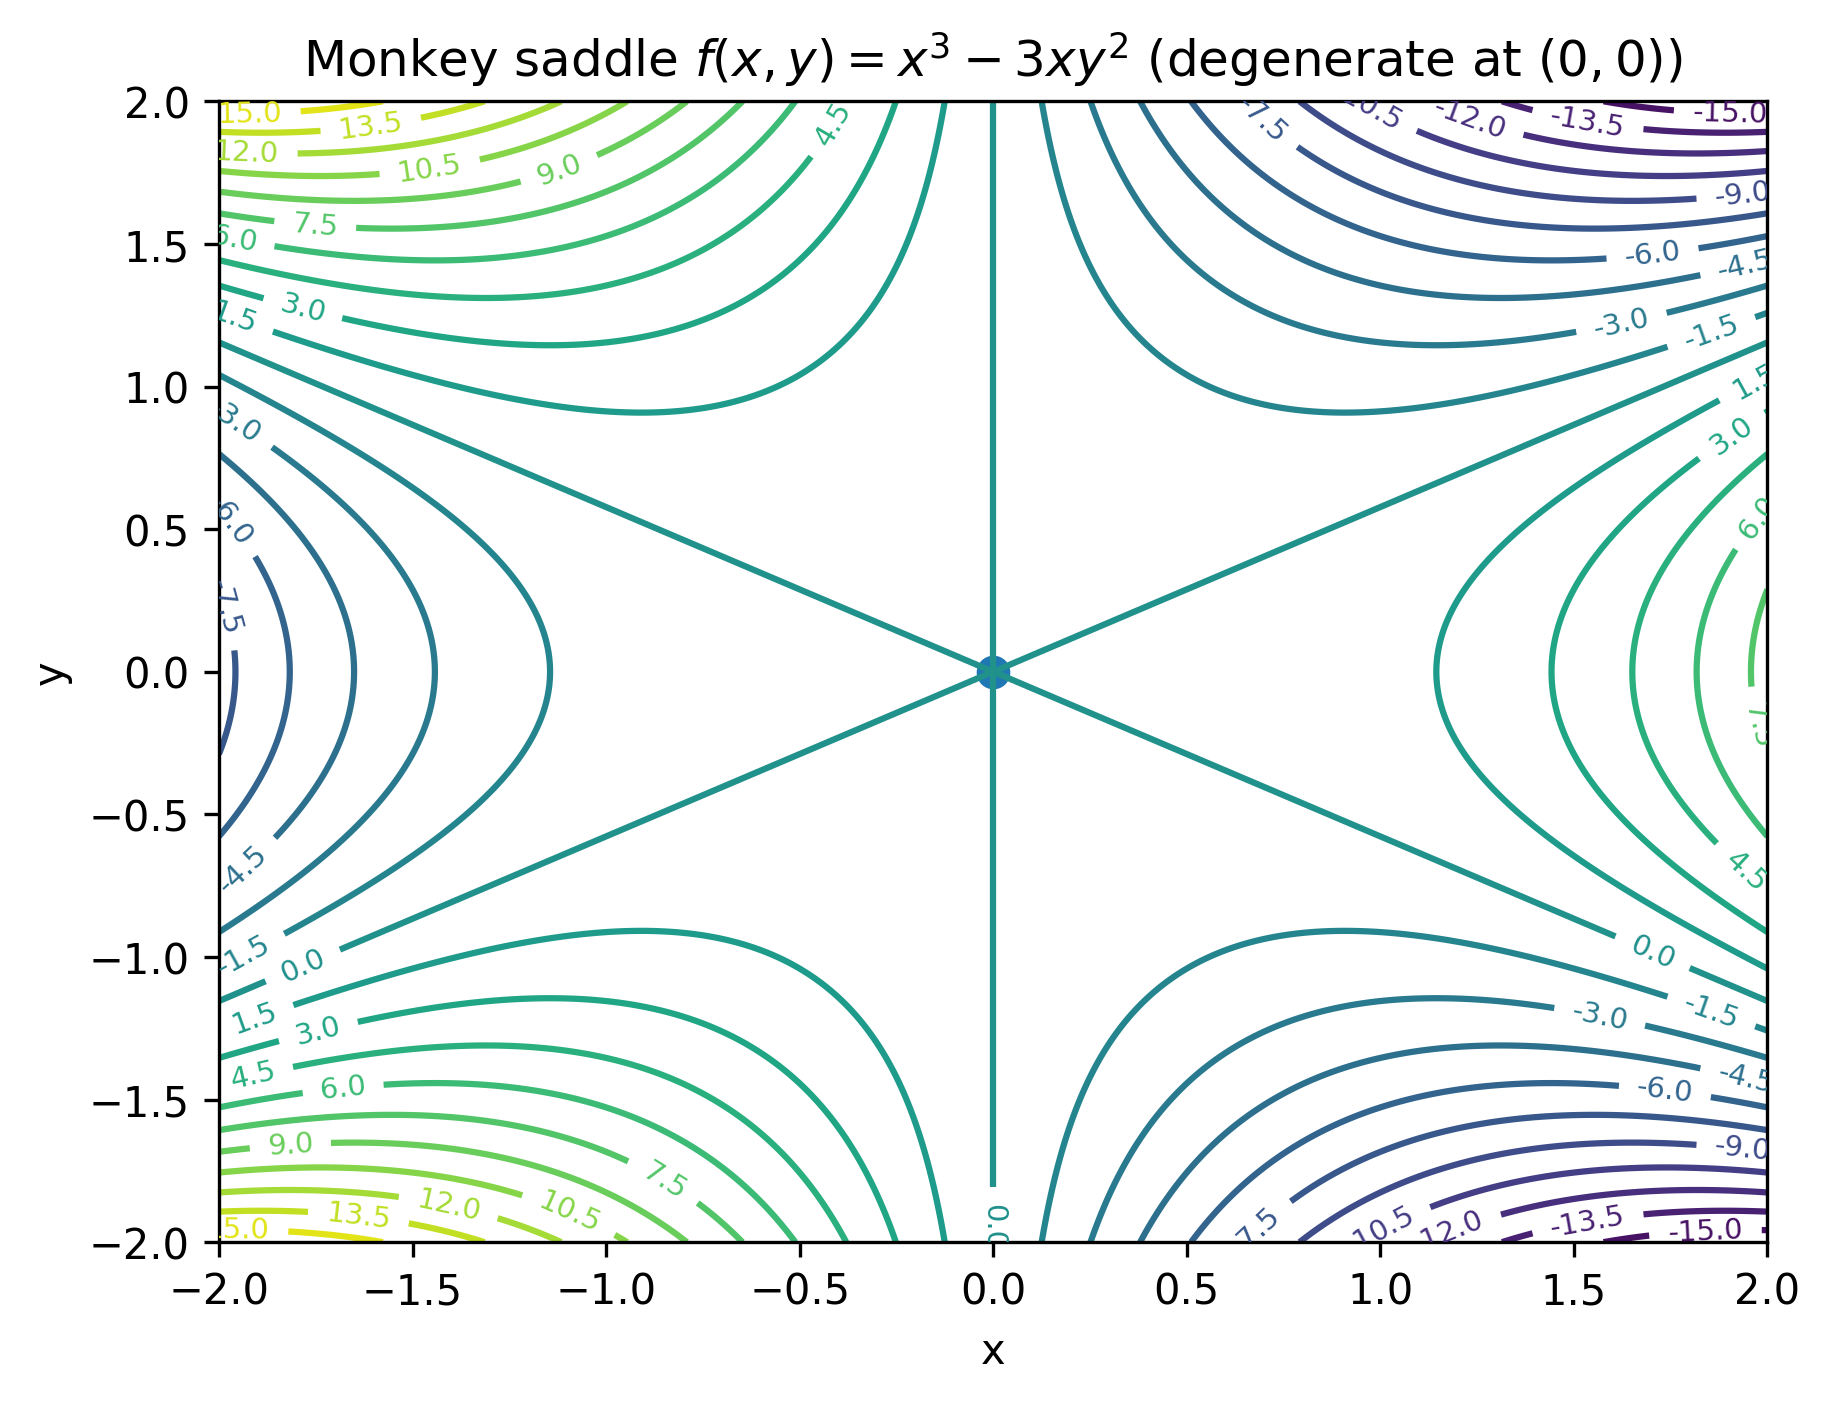
\includegraphics[width=0.78\linewidth]{chapters/part07_volume_vii/figures/morse_fig1_monkey_saddle_contours.png}
		\caption{Example of a degenerate critical point: the monkey saddle $f(x,y)=x^3-3xy^2$ has a critical point at $(0,0)$ with degenerate Hessian.}
	\end{figure}
	
	\begin{figure}[htbp]
		\centering
		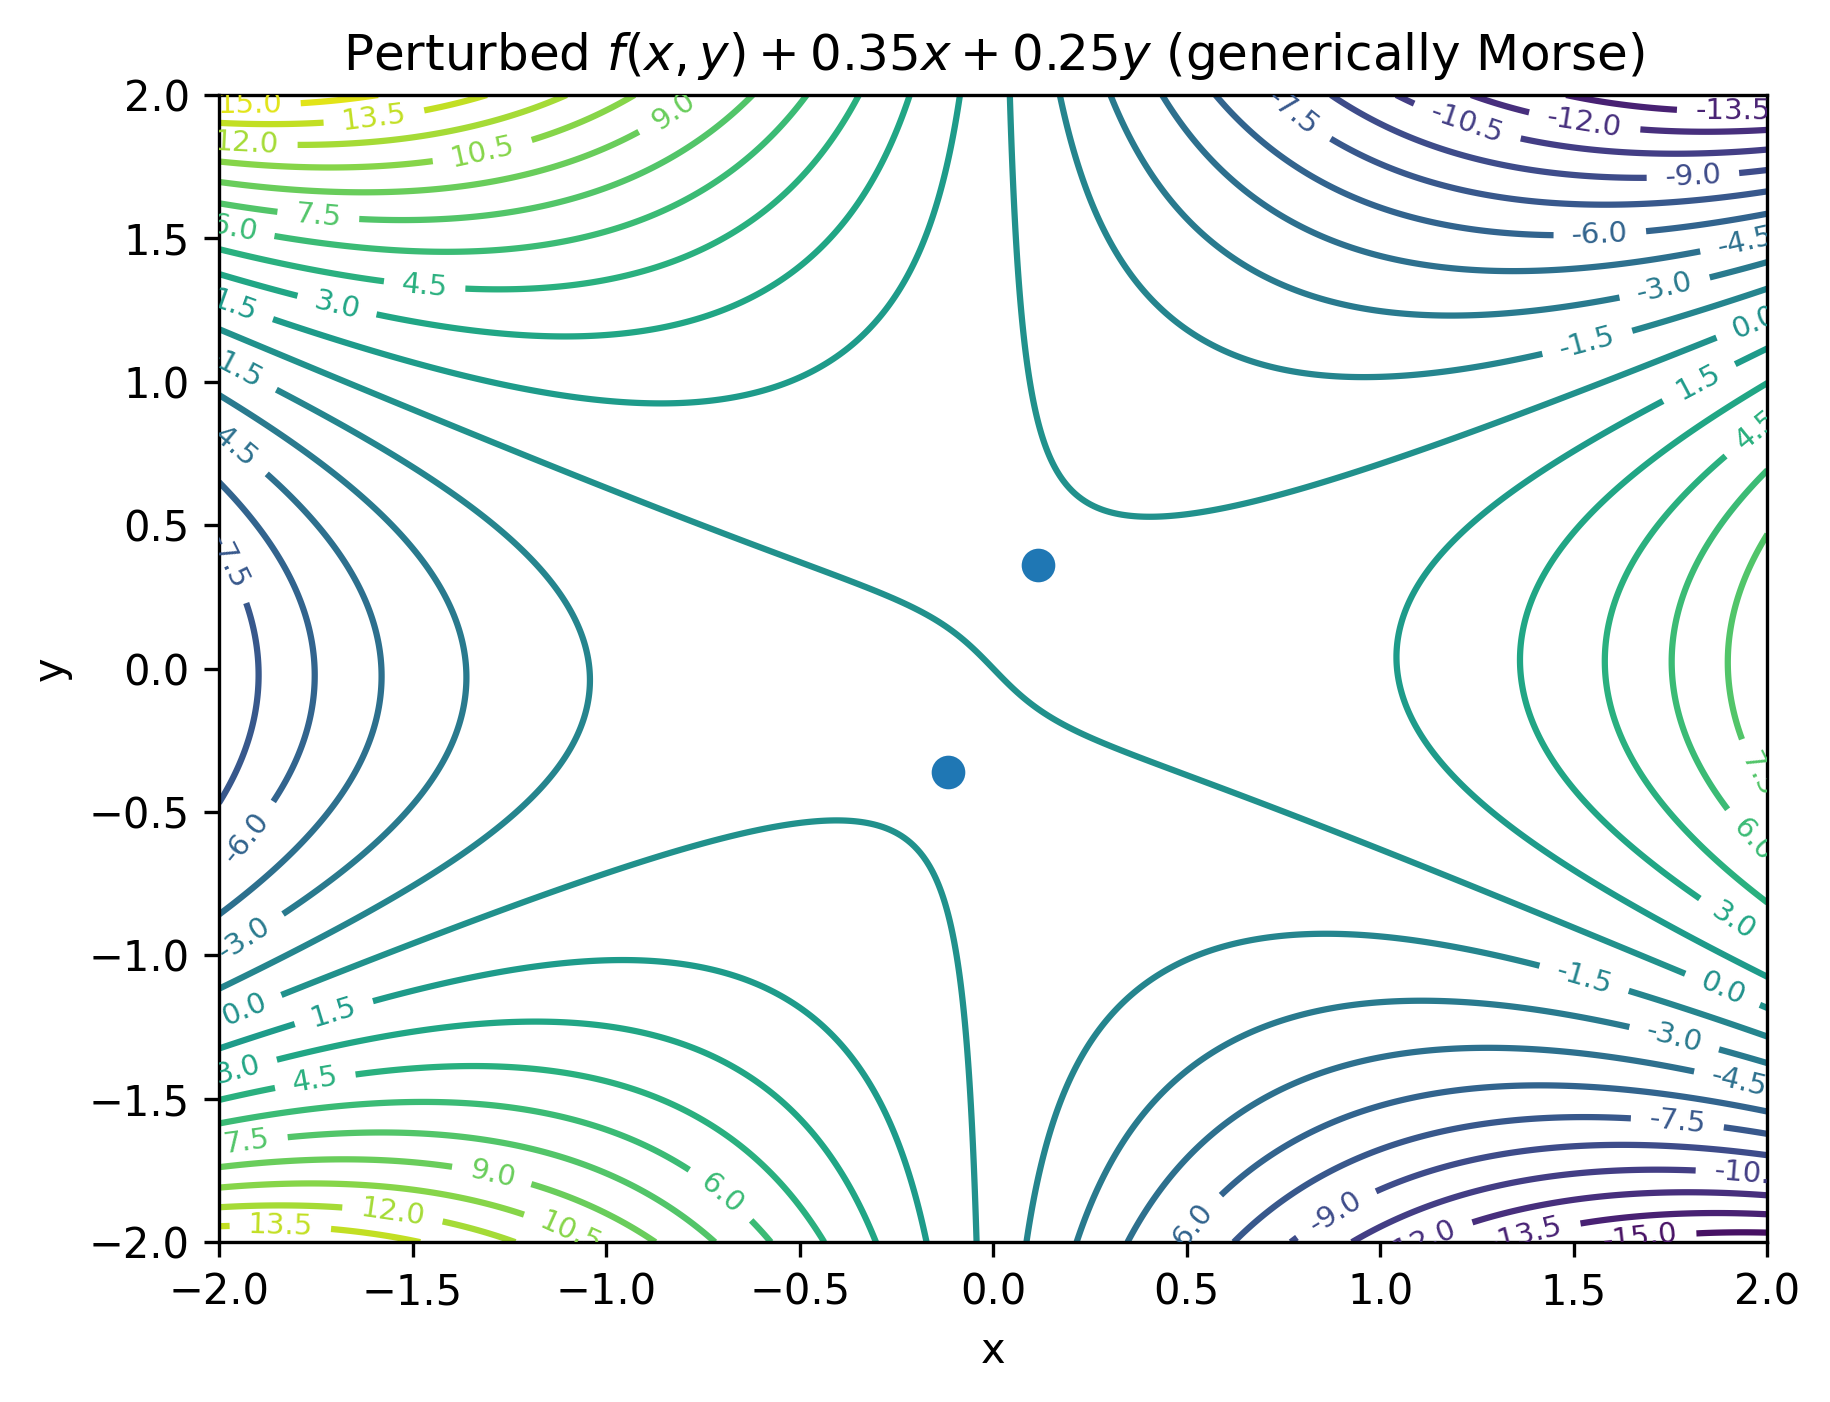
\includegraphics[width=0.78\linewidth]{chapters/part07_volume_vii/figures/morse_fig2_perturbed_contours.png}
		\caption{Generic linear perturbation $f_a=f+ax+by$ produces isolated non-degenerate critical points (Morse).}
	\end{figure}
	
	\begin{figure}[htbp]
		\centering
		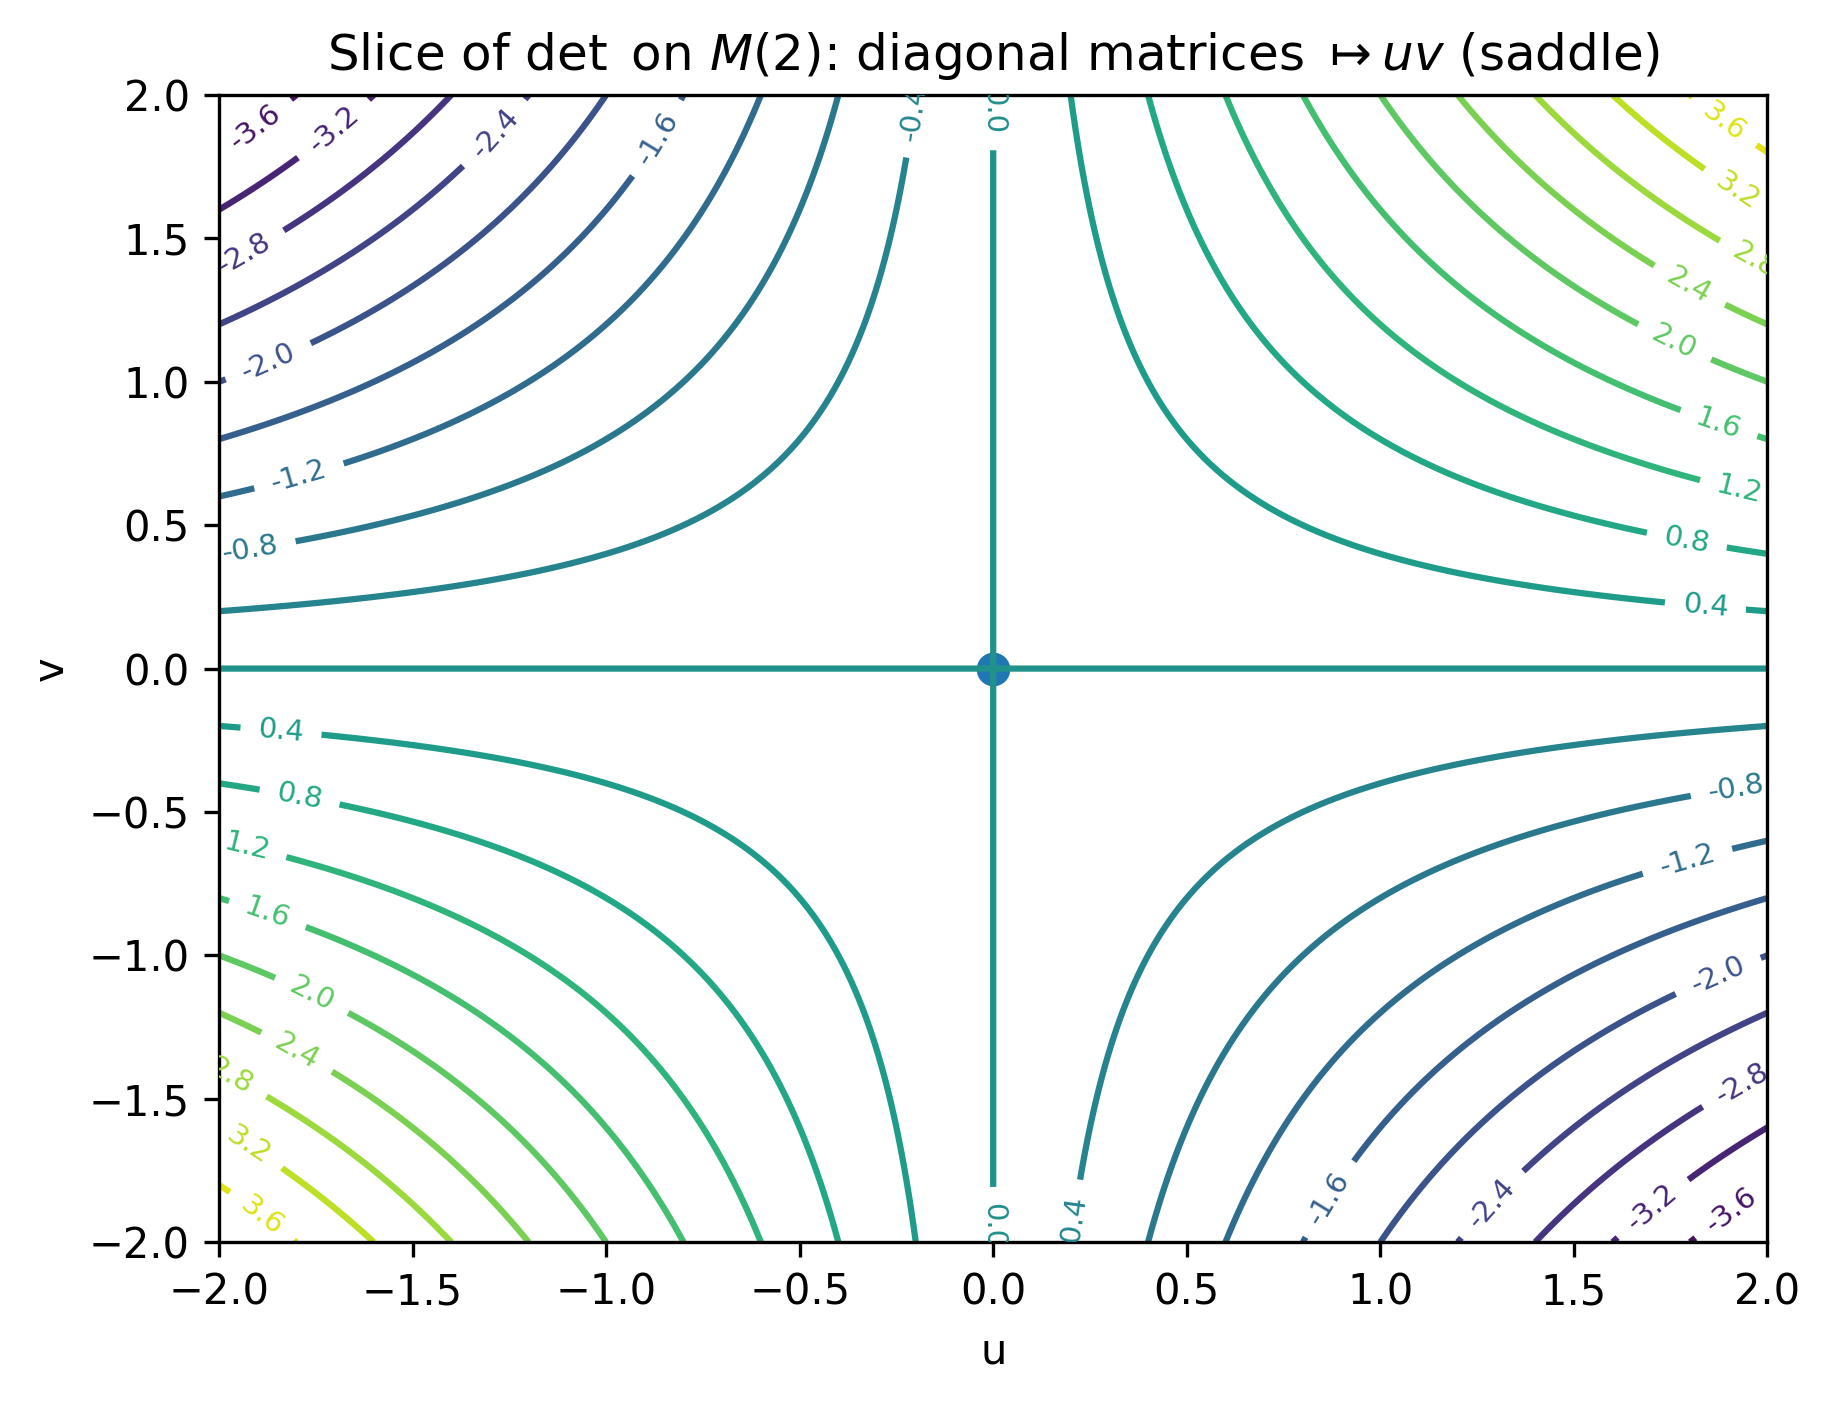
\includegraphics[width=0.78\linewidth]{chapters/part07_volume_vii/figures/morse_fig3_det_M2_slice_uv.png}
		\caption{For $n=2$, a diagonal slice of $\det$ is $uv$, which has a non-degenerate saddle critical point at $(0,0)$.}
	\end{figure}
	
	\par\medskip\noindent\textbf{How to recognize critical, non-degenerate, and degenerate critical points}\par\smallskip

	
	\noindent\textbf{Critical points.}
	Let $f:\mathbb{R}^k\to\mathbb{R}$ be smooth. A point $x_0\in\mathbb{R}^k$ is a \emph{critical point} of $f$ if
	\[
	df_{x_0}=0.
	\]
	In standard coordinates this is equivalent to vanishing of all first partial derivatives:
	\[
	\nabla f(x_0)=0
	\qquad\Longleftrightarrow\qquad
	\frac{\partial f}{\partial x_1}(x_0)=\cdots=\frac{\partial f}{\partial x_k}(x_0)=0.
	\]
	Geometrically, this means that the first-order change of $f$ at $x_0$ is zero in every direction: there is no
	``instant'' increase or decrease to first order.
	
	\medskip
	\noindent\textbf{Non-degenerate vs.\ degenerate.}
	Assume $x_0$ is a critical point. The \emph{Hessian matrix} of $f$ at $x_0$ is
	\[
	H_f(x_0)=\left(\frac{\partial^2 f}{\partial x_i\,\partial x_j}(x_0)\right)_{1\le i,j\le k}.
	\]
	\begin{itemize}
		\item The critical point $x_0$ is called \emph{non-degenerate} if
		\[
		\det\big(H_f(x_0)\big)\neq 0.
		\]
		Equivalently, $H_f(x_0)$ is invertible. In this case the quadratic (second-order) approximation of $f$ at $x_0$
		has genuine curvature in all directions (no ``flat'' direction survives).
		
		\item The critical point $x_0$ is called \emph{degenerate} if
		\[
		\det\big(H_f(x_0)\big)=0.
		\]
		Equivalently, $H_f(x_0)$ has a nontrivial kernel, so there exists a nonzero direction $v$ such that the quadratic form
		$v^T H_f(x_0) v$ vanishes. In this case second-order information is not sufficient to determine the local shape, and
		higher-order terms in the Taylor expansion may dominate.
	\end{itemize}
	
	\medskip
	\par\medskip\noindent\textbf{Example 1: a degenerate critical point (monkey saddle)}\par\smallskip

	Consider
	\[
	f(x,y)=x^3-3xy^2.
	\]
	\noindent\textbf{Step 1: critical point.}
	Compute the first derivatives:
	\[
	f_x(x,y)=3x^2-3y^2,
	\qquad
	f_y(x,y)=-6xy.
	\]
	At $(0,0)$ we have
	\[
	f_x(0,0)=0,\qquad f_y(0,0)=0,
	\]
	so $(0,0)$ is a critical point.
	
	\smallskip
	\noindent\textbf{Step 2: degeneracy.}
	Compute the second derivatives:
	\[
	f_{xx}(x,y)=6x,\qquad f_{xy}(x,y)=-6y,\qquad f_{yy}(x,y)=-6x.
	\]
	Thus
	\[
	H_f(x,y)=
	\begin{pmatrix}
		6x & -6y\\
		-6y & -6x
	\end{pmatrix},
	\qquad
	H_f(0,0)=
	\begin{pmatrix}
		0 & 0\\
		0 & 0
	\end{pmatrix}.
	\]
	Hence
	\[
	\det(H_f(0,0))=0,
	\]
	so the critical point $(0,0)$ is \emph{degenerate}. Intuitively, this happens because the Taylor expansion of $f$ at
	$(0,0)$ starts with cubic terms: the quadratic part vanishes completely.
	
	\medskip
	\par\medskip\noindent\textbf{Example 2: a non-degenerate critical point (a saddle)}\par\smallskip

	Consider
	\[
	g(u,v)=uv.
	\]
	\noindent\textbf{Step 1: critical point.}
	The gradient is
	\[
	\nabla g(u,v)=(g_u(u,v),g_v(u,v))=(v,u).
	\]
	Thus $\nabla g(0,0)=(0,0)$, so $(0,0)$ is a critical point.
	
	\smallskip
	\noindent\textbf{Step 2: non-degeneracy.}
	The second derivatives are
	\[
	g_{uu}=0,\qquad g_{uv}=1,\qquad g_{vv}=0,
	\]
	so the Hessian matrix is constant:
	\[
	H_g=
	\begin{pmatrix}
		0 & 1\\
		1 & 0
	\end{pmatrix},
	\qquad
	\det(H_g)=-1\neq 0.
	\]
	Therefore $(0,0)$ is a \emph{non-degenerate} critical point (in fact, a saddle point). This is the local model
	that appears in the case $n=2$ for the determinant function on $M(2)$ (restricted to diagonal matrices).
	
	\par\medskip\noindent\textbf{Geometric meaning of a critical point (``horizontal tangent plane'')}\par\smallskip

	
	\noindent
	Let $f:\mathbb{R}^k\to\mathbb{R}$ be smooth and let $x_0\in\mathbb{R}^k$.
	The condition that $x_0$ is a critical point is
	\[
	\nabla f(x_0)=0
	\qquad\Longleftrightarrow\qquad
	df_{x_0}=0.
	\]
	Geometrically, this means that the \emph{first-order} (linear) change of $f$ at $x_0$ vanishes in every direction.
	
	\medskip
	\noindent\textbf{(1) The tangent approximation.}
	For a small vector $h\in\mathbb{R}^k$, Taylor's formula gives
	\[
	f(x_0+h)=f(x_0)+\nabla f(x_0)\cdot h+\frac12\,h^T H_f(x_0)\,h+\text{(higher order terms)}.
	\]
	The term $\nabla f(x_0)\cdot h$ is the \emph{first-order slope}.
	Thus if $\nabla f(x_0)=0$, then
	\[
	f(x_0+h)=f(x_0)+\frac12\,h^T H_f(x_0)\,h+\cdots,
	\]
	so $f$ does not change to first order when we move away from $x_0$; the first nontrivial change begins at second order
	(or at even higher order if the critical point is degenerate).
	
	\medskip
	\noindent\textbf{(2) The case $k=2$: a surface in $\mathbb{R}^3$.}
	If $f(x,y)$ is a function of two variables, its graph is the surface
	\[
	S=\{(x,y,z)\in\mathbb{R}^3:\ z=f(x,y)\}.
	\]
	At a point $(x_0,y_0)$ the tangent plane to $S$ is
	\[
	z=f(x_0,y_0)+f_x(x_0,y_0)(x-x_0)+f_y(x_0,y_0)(y-y_0).
	\]
	Hence $(x_0,y_0)$ is critical iff $f_x(x_0,y_0)=f_y(x_0,y_0)=0$, and then the tangent plane simplifies to
	\[
	z=f(x_0,y_0),
	\]
	which is a \emph{horizontal plane}. This is the precise meaning of the phrase
	``the tangent plane is horizontal at a critical point.''
	
	\medskip
	\noindent\textbf{(3) What you see on a contour plot.}
	A contour plot draws level sets $f(x,y)=c$. If $\nabla f(x_0,y_0)\neq 0$, then nearby level curves are smooth and
	their normal direction is given by the gradient. If $\nabla f(x_0,y_0)=0$, the point can become a special point of
	the level sets: for a non-degenerate minimum/maximum one typically sees small closed curves around $(x_0,y_0)$, for a
	saddle one sees level curves crossing, and for degenerate critical points one can see multi-armed or ``pinched''
	patterns (e.g.\ the monkey saddle).
	
	\medskip
	\noindent\textbf{Figures.}
	
	\begin{figure}[htbp]
		\centering
		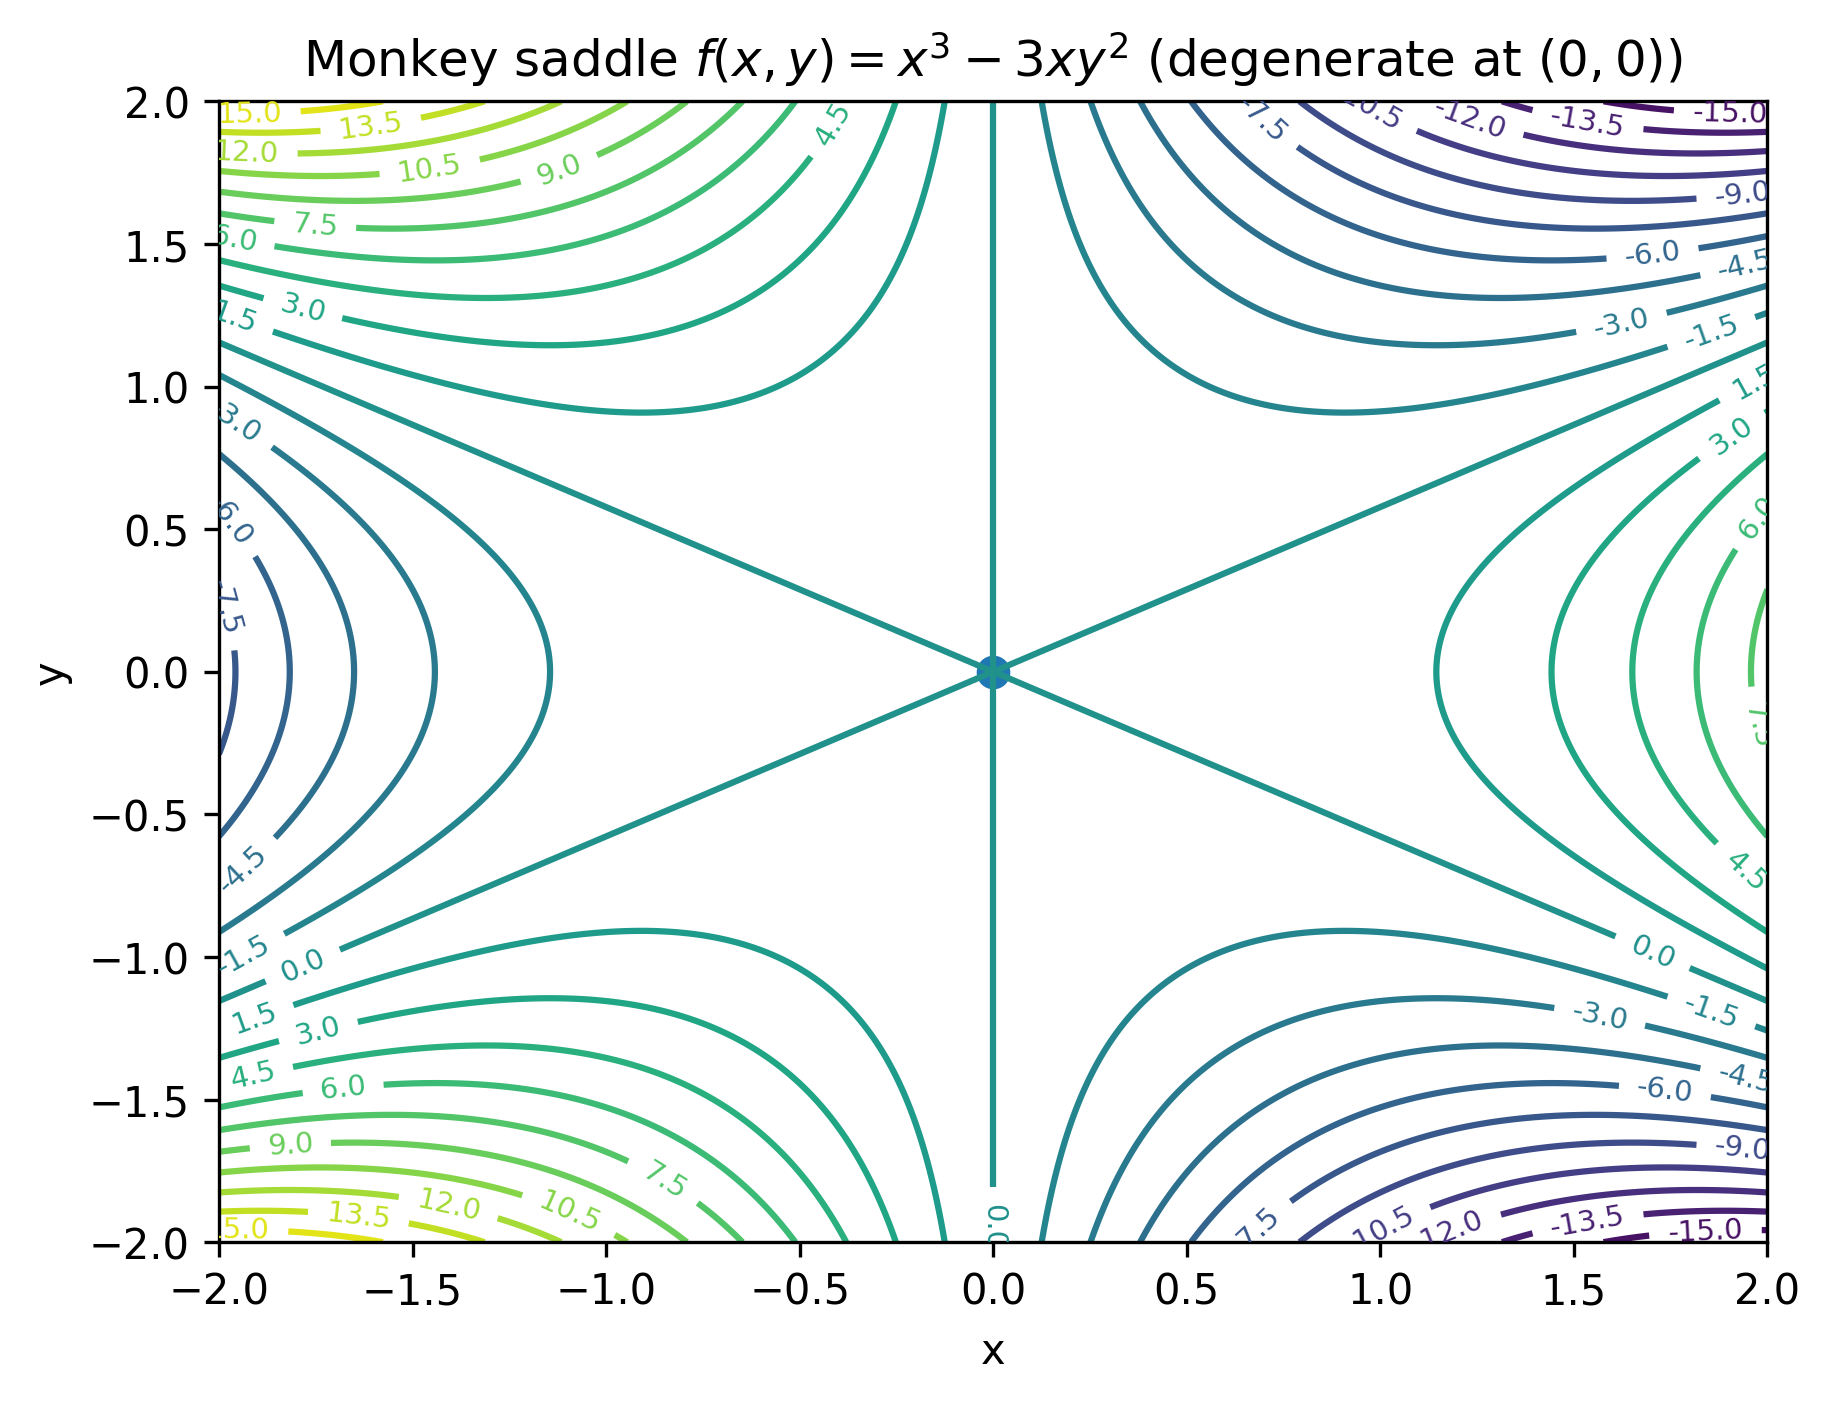
\includegraphics[width=0.78\linewidth]{chapters/part07_volume_vii/figures/morse_fig1_monkey_saddle_contours.png}
		\caption{Contour plot of the monkey saddle $f(x,y)=x^3-3xy^2$: $(0,0)$ is critical and degenerate (the quadratic part vanishes).}
	\end{figure}
	
	\begin{figure}[htbp]
		\centering
		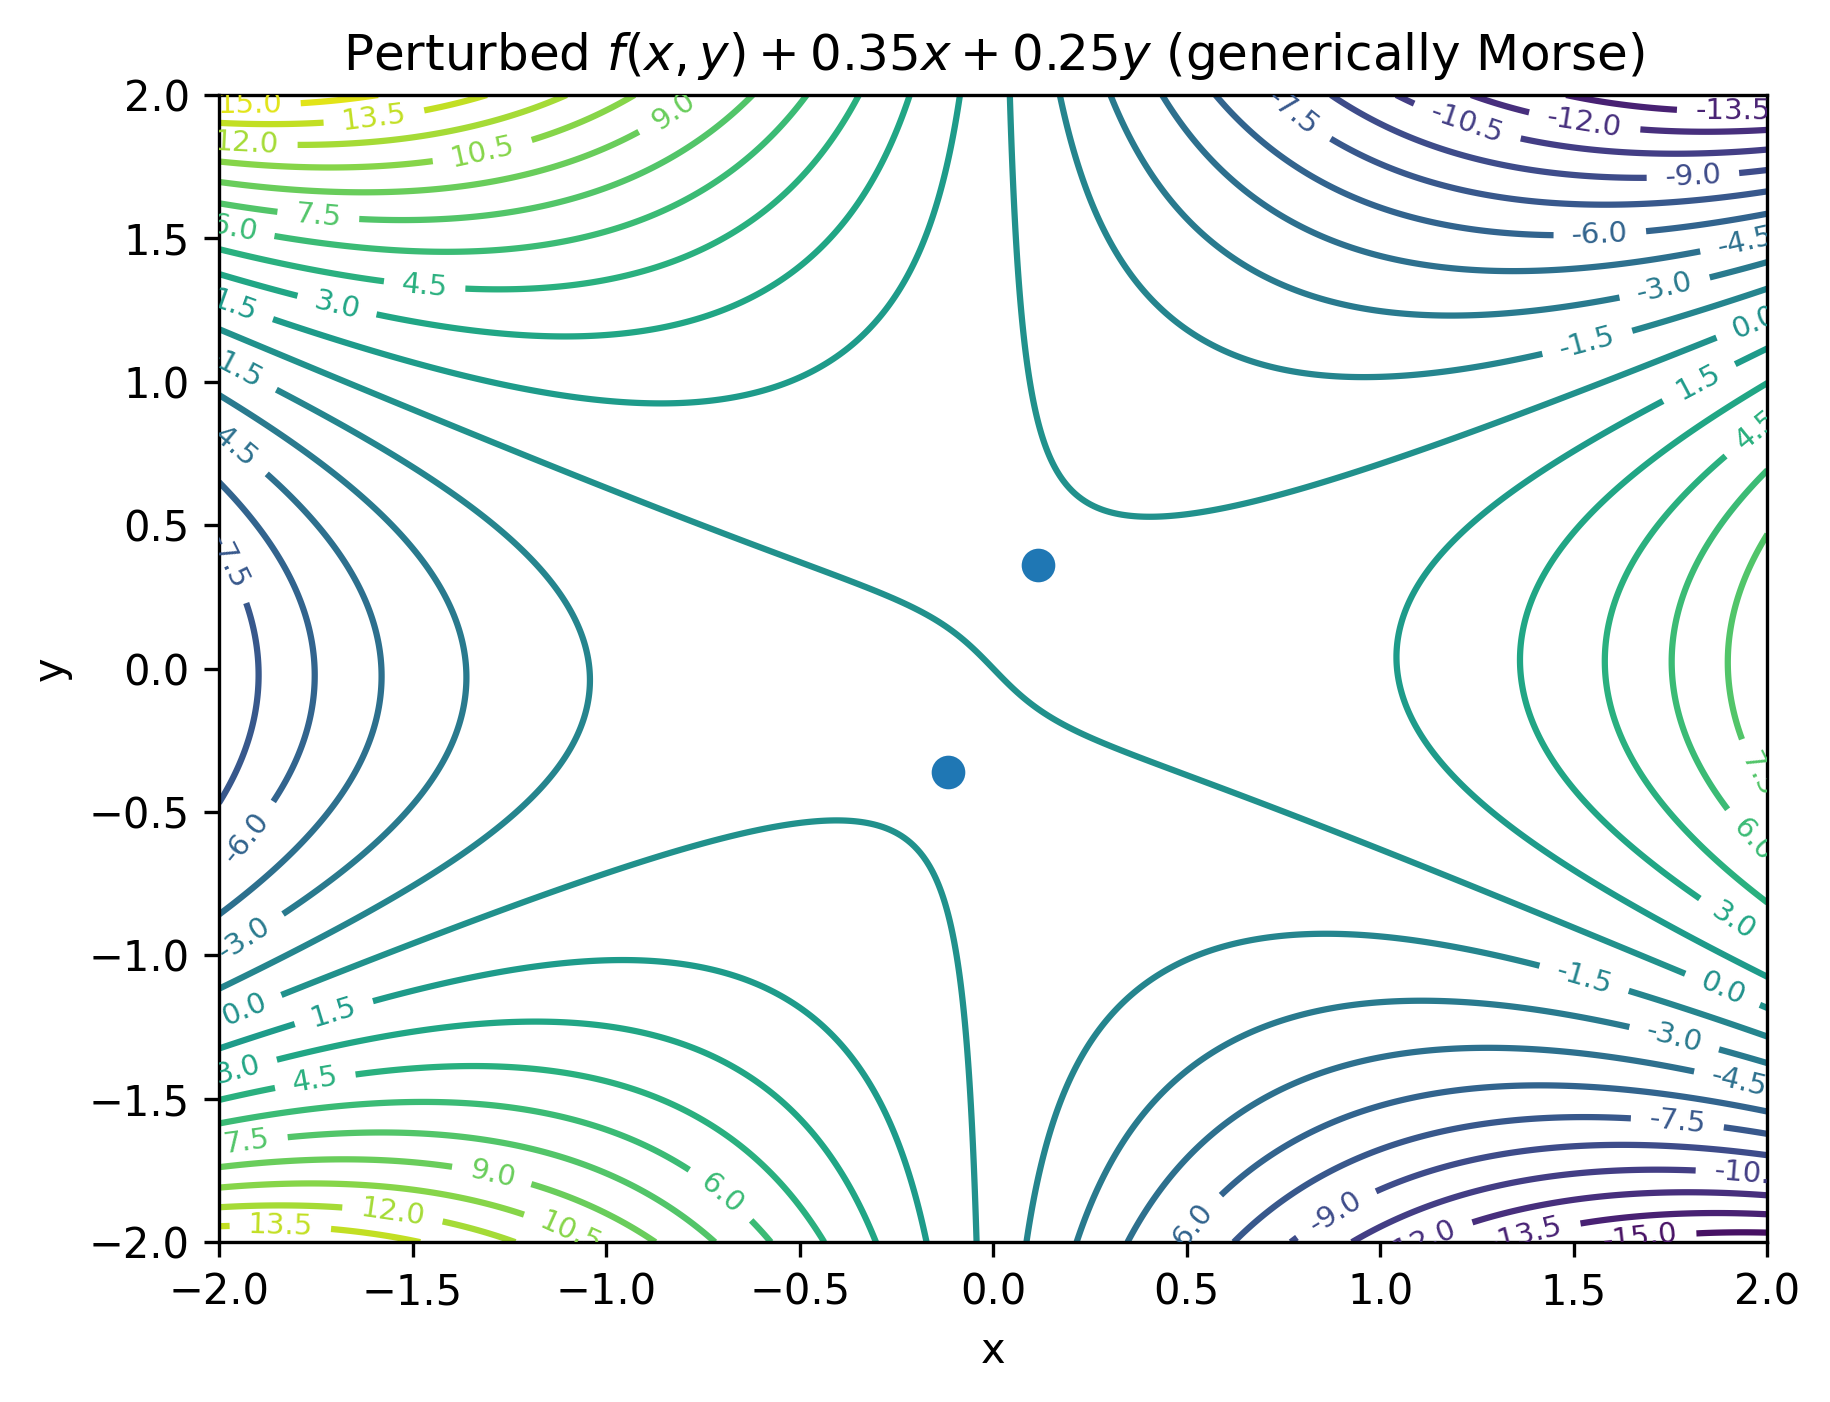
\includegraphics[width=0.78\linewidth]{chapters/part07_volume_vii/figures/morse_fig2_perturbed_contours.png}
		\caption{Generic linear perturbation $f_a=f+ax+by$ produces isolated non-degenerate critical points (a Morse function).}
	\end{figure}
	
	\begin{figure}[htbp]
		\centering
		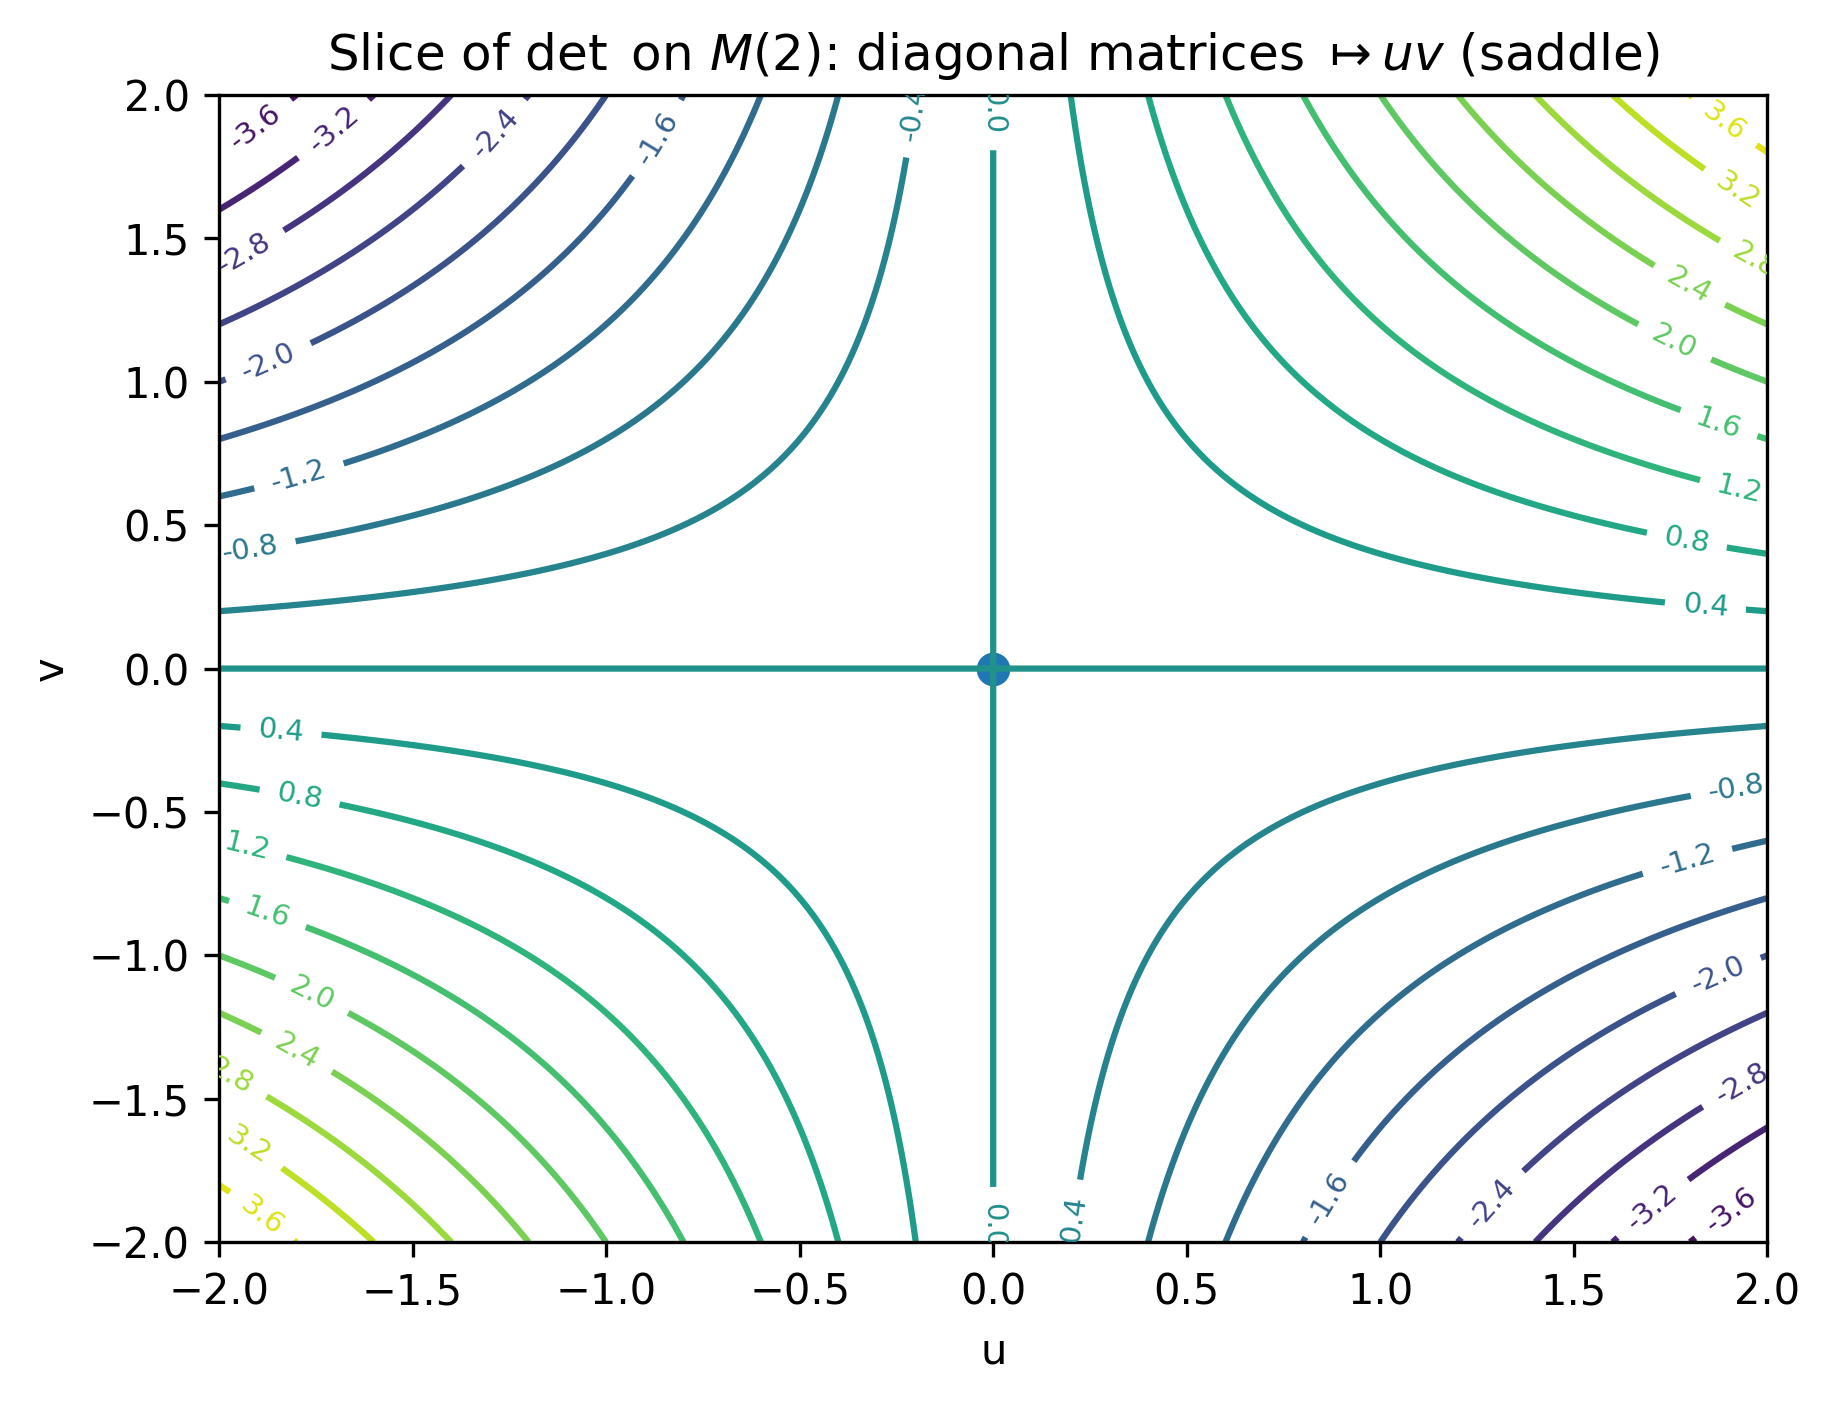
\includegraphics[width=0.78\linewidth]{chapters/part07_volume_vii/figures/morse_fig3_det_M2_slice_uv.png}
		\caption{A diagonal slice of $\det$ on $M(2)$ equals $uv$ and has a non-degenerate saddle critical point at $(0,0)$.}
	\end{figure}
	
	% ------------------------------------------------------------
	% Taylor expansion and the meaning of (non)degeneracy in 1D and 2D
	% ------------------------------------------------------------
	
	\par\medskip\noindent\textbf{Taylor expansion, saddles, and degeneracy (1D and 2D)}\par\smallskip

	
	\noindent\textbf{1D: critical points and the second derivative test.}
	Let $f:\mathbb{R}\to\mathbb{R}$ be $C^2$ and let $x_0\in\mathbb{R}$.
	A \emph{critical point} is a point where
	\[
	f'(x_0)=0.
	\]
	Taylor's theorem (with remainder) gives, for $x$ near $x_0$,
	\[
	f(x)=f(x_0)+f'(x_0)(x-x_0)+\frac12 f''(x_0)(x-x_0)^2 + o\!\left((x-x_0)^2\right).
	\]
	At a critical point $f'(x_0)=0$, so
	\[
	f(x)=f(x_0)+\frac12 f''(x_0)(x-x_0)^2 + o\!\left((x-x_0)^2\right).
	\]
	Hence:
	\begin{itemize}
		\item If $f''(x_0)>0$, then $x_0$ is a \emph{strict local minimum}.
		\item If $f''(x_0)<0$, then $x_0$ is a \emph{strict local maximum}.
		\item If $f''(x_0)=0$, the second derivative test is \emph{inconclusive}; one must use higher-order terms or other methods.
	\end{itemize}
	
	\medskip
	\noindent\textbf{1D: why $x^2$ and $x^4$ differ near $0$.}
	Consider $f(x)=x^2$ and $g(x)=x^4$ at $0$:
	\[
	f(0)=0,\quad f'(0)=0,\quad f''(0)=2\neq 0,
	\]
	so the \emph{first nonzero Taylor term} is quadratic:
	\[
	f(x)=x^2.
	\]
	For $g(x)=x^4$,
	\[
	g(0)=0,\quad g'(0)=0,\quad g''(0)=0,\quad g^{(3)}(0)=0,\quad g^{(4)}(0)=24\neq 0,
	\]
	so the first nonzero Taylor term appears at order $4$:
	\[
	g(x)=\frac{1}{4!}g^{(4)}(0)x^4=x^4.
	\]
	This explains the geometric behavior: $x^4$ is \emph{much flatter near $0$} (since for small $|x|$ we have $|x|^4\ll |x|^2$), even though it grows faster for large $|x|$.
	
	\bigskip
	\noindent\textbf{2D: extended Taylor expansion and the Hessian.}
	Let $f:\mathbb{R}^2\to\mathbb{R}$ be $C^2$ and let $p=(a,b)$.
	Write $h=(h_1,h_2)=(x-a,y-b)$. Then Taylor's theorem in $\mathbb{R}^2$ gives
	\[
	f(p+h)
	=
	f(p)
	+
	\nabla f(p)\cdot h
	+
	\frac12\, h^\top H_f(p)\, h
	+
	o\!\left(\|h\|^2\right),
	\]
	where
	\[
	\nabla f(p)=
	\begin{pmatrix}
		f_x(p)\\[2pt]
		f_y(p)
	\end{pmatrix},
	\qquad
	H_f(p)=
	\begin{pmatrix}
		f_{xx}(p) & f_{xy}(p)\\[2pt]
		f_{yx}(p) & f_{yy}(p)
	\end{pmatrix},
	\]
	and
	\[
	h^\top H_f(p)\,h
	=
	f_{xx}(p)\,h_1^2 + 2f_{xy}(p)\,h_1h_2 + f_{yy}(p)\,h_2^2.
	\]
	
	\medskip
	\noindent\textbf{Critical points and leading-order shape.}
	A point $p$ is a \emph{critical point} iff
	\[
	\nabla f(p)=0.
	\]
	At a critical point the linear term vanishes, and the first term controlling the local geometry is the quadratic form
	\[
	Q(h)=\frac12\, h^\top H_f(p)\,h.
	\]
	This is the multivariable analogue of using $f''(x_0)$ in 1D.
	
	\medskip
	\noindent\textbf{Nondegenerate vs degenerate critical points.}
	\begin{itemize}
		\item $p$ is \emph{nondegenerate} if the Hessian is invertible:
		\[
		\det H_f(p)\neq 0.
		\]
		\item $p$ is \emph{degenerate} if the Hessian is singular:
		\[
		\det H_f(p)=0.
		\]
		In this case the quadratic approximation does \emph{not} fully determine the local shape; higher-order terms are needed.
	\end{itemize}
	
	\medskip
	\noindent\textbf{2D classification via the determinant test (nondegenerate case).}
	At a critical point $p$, set
	\[
	D=\det H_f(p)=f_{xx}(p)f_{yy}(p)-f_{xy}(p)^2.
	\]
	Then:
	\begin{itemize}
		\item If $D>0$ and $f_{xx}(p)>0$, then $p$ is a \emph{strict local minimum}.
		\item If $D>0$ and $f_{xx}(p)<0$, then $p$ is a \emph{strict local maximum}.
		\item If $D<0$, then $H_f(p)$ is \emph{indefinite} and $p$ is a \emph{saddle point}.
		\item If $D=0$, the test is \emph{inconclusive} (the point is degenerate).
	\end{itemize}
	
	\bigskip
	\noindent\textbf{Saddles vs degeneracy: key examples.}
	
	\medskip
	\noindent\emph{(1) Nondegenerate saddle.}
	Let
	\[
	f(x,y)=x^2-y^2.
	\]
	Then $(0,0)$ is critical and
	\[
	H_f(0,0)=
	\begin{pmatrix}
		2 & 0\\
		0 & -2
	\end{pmatrix},
	\qquad
	\det H_f(0,0)=-4<0.
	\]
	Hence $(0,0)$ is a \emph{nondegenerate saddle}. Geometrically, the surface bends upward in the $x$-direction and downward in the $y$-direction.
	
	\medskip
	\noindent\emph{(2) Degenerate saddle.}
	Let
	\[
	g(x,y)=x^4-y^4.
	\]
	Then $(0,0)$ is critical, and all second partial derivatives vanish at $(0,0)$, so
	\[
	H_g(0,0)=0,
	\qquad
	\det H_g(0,0)=0,
	\]
	i.e.\ $(0,0)$ is \emph{degenerate}. Nevertheless it is still a \emph{saddle} because
	\[
	g(x,0)=x^4\ge 0,
	\qquad
	g(0,y)=-y^4\le 0,
	\]
	so arbitrarily close to $(0,0)$ one finds points where $g>0$ and points where $g<0$.
	
	\medskip
	\noindent\emph{(3) Degenerate minimum (flat bottom).}
	Let
	\[
	h(x,y)=x^4+y^4.
	\]
	Then $(0,0)$ is critical and degenerate ($H_h(0,0)=0$), but $h(x,y)\ge 0$ with equality only at $(0,0)$, so $(0,0)$ is a \emph{(degenerate) strict local minimum}.
	
	\medskip
	\noindent\textbf{Moral.}
	\begin{itemize}
		\item \emph{Saddle} means: the function takes values both above and below $f(p)$ arbitrarily close to $p$.
		\item \emph{Degenerate} means: the quadratic (Hessian) term is insufficient ($\det H_f(p)=0$).
		\item Saddles can be nondegenerate (e.g.\ $x^2-y^2$) or degenerate (e.g.\ $x^4-y^4$).
	\end{itemize}
	
	% -------------------- Figures: saddles (nondegenerate vs degenerate) --------------------
	% Put the PNG files in your project folder, e.g. in: figs/
	% and adjust the paths below if needed.
	
	\par\medskip\noindent\textbf{Figures: nondegenerate vs degenerate saddle}\par\smallskip

	
	\begin{figure}[htbp]
		\centering
		\begin{minipage}{0.49\linewidth}
			\centering
			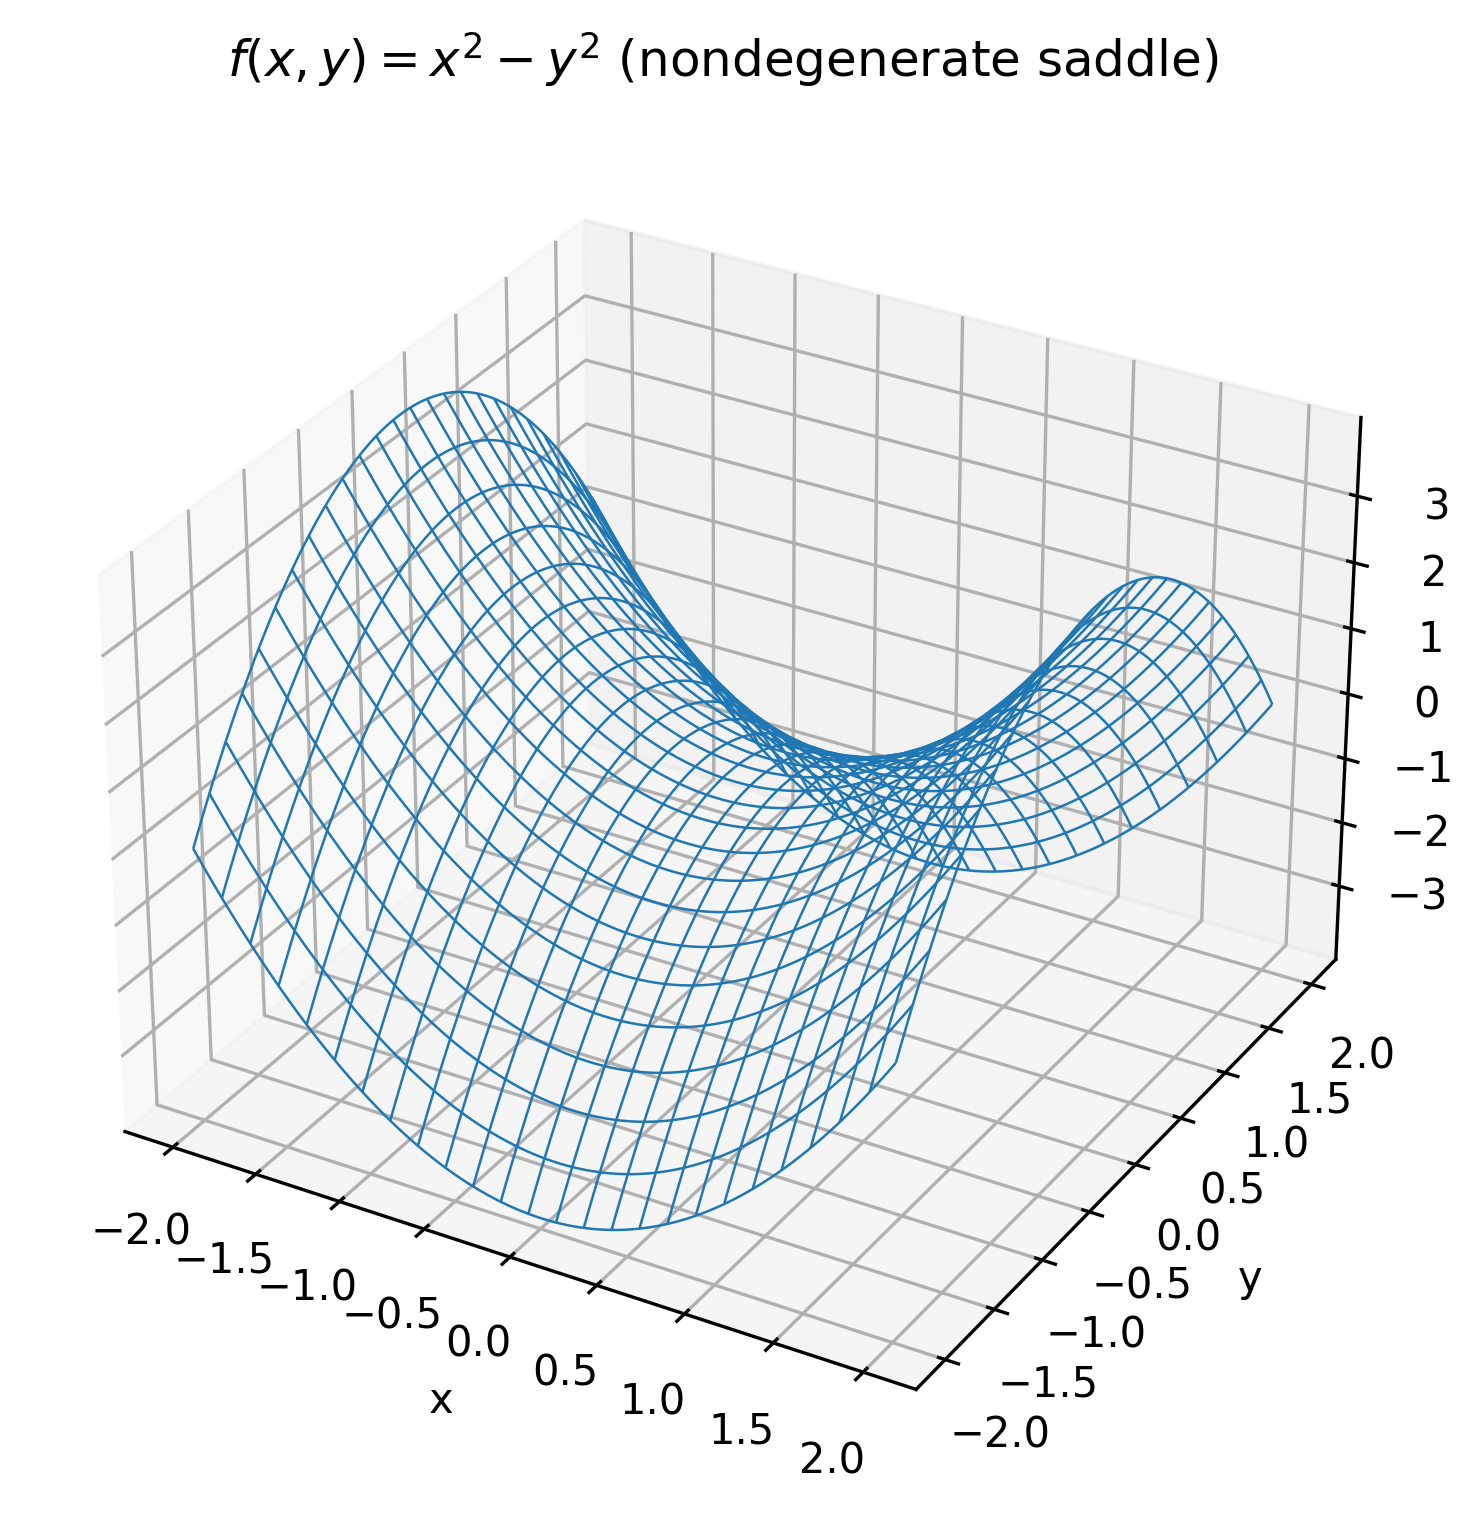
\includegraphics[width=\linewidth]{chapters/part07_volume_vii/figures/fig_saddle_x2_minus_y2_surface.png}
			\caption*{$f(x,y)=x^2-y^2$: 3D surface (nondegenerate saddle).}
		\end{minipage}\hfill
		\begin{minipage}{0.49\linewidth}
			\centering
			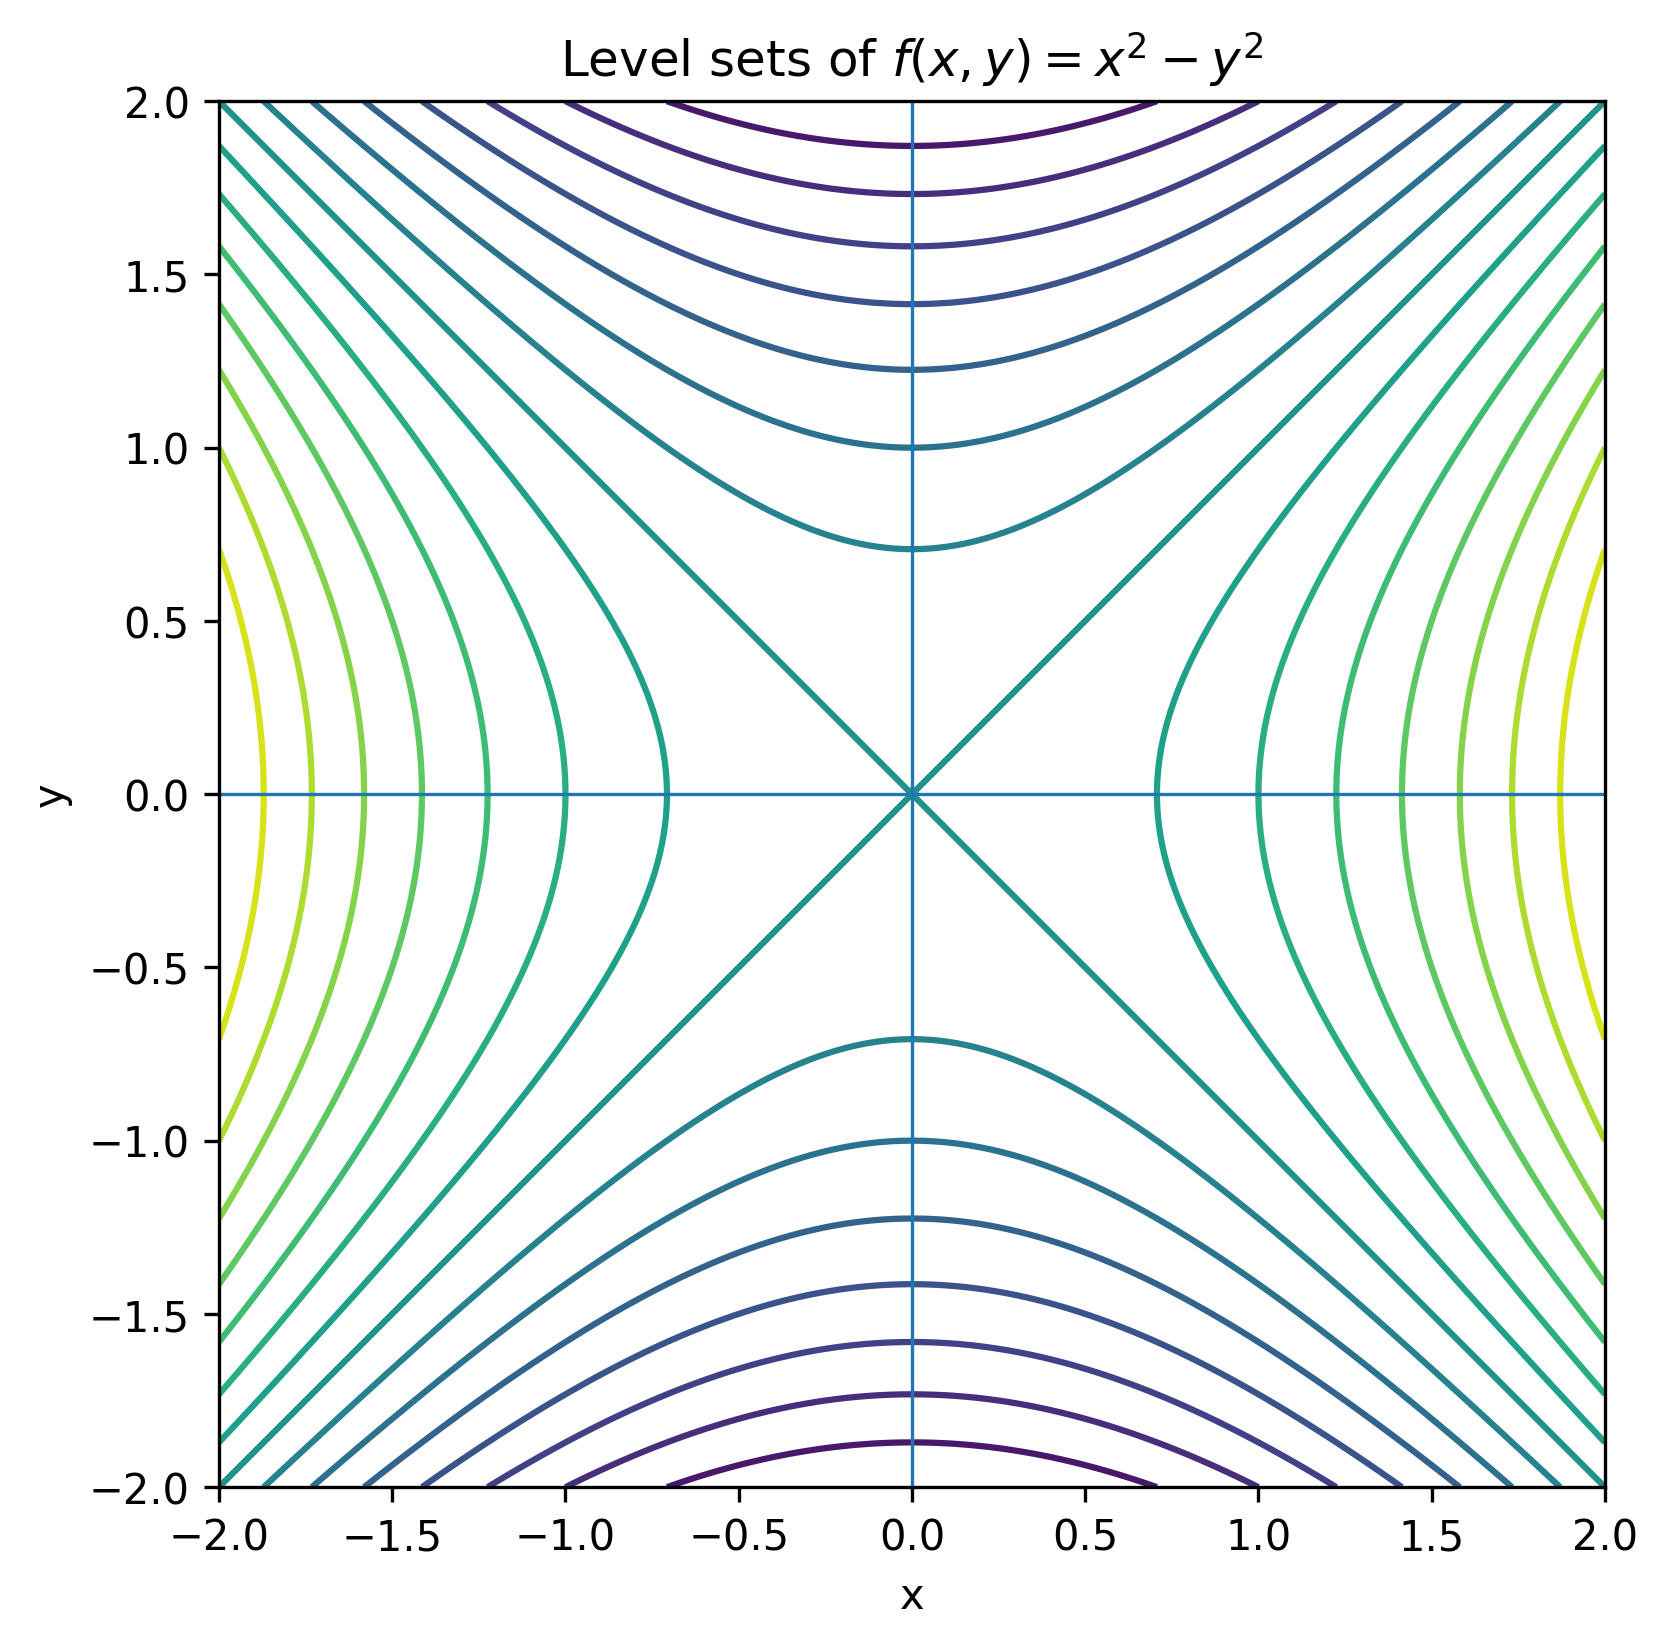
\includegraphics[width=\linewidth]{chapters/part07_volume_vii/figures/fig_saddle_x2_minus_y2_contours.png}
			\caption*{$f(x,y)=x^2-y^2$: level sets (hyperbolas).}
		\end{minipage}
		\caption{A nondegenerate saddle: curvature is already visible at quadratic order (Hessian indefinite).}
	\end{figure}
	
	\begin{figure}[htbp]
		\centering
		\begin{minipage}{0.49\linewidth}
			\centering
			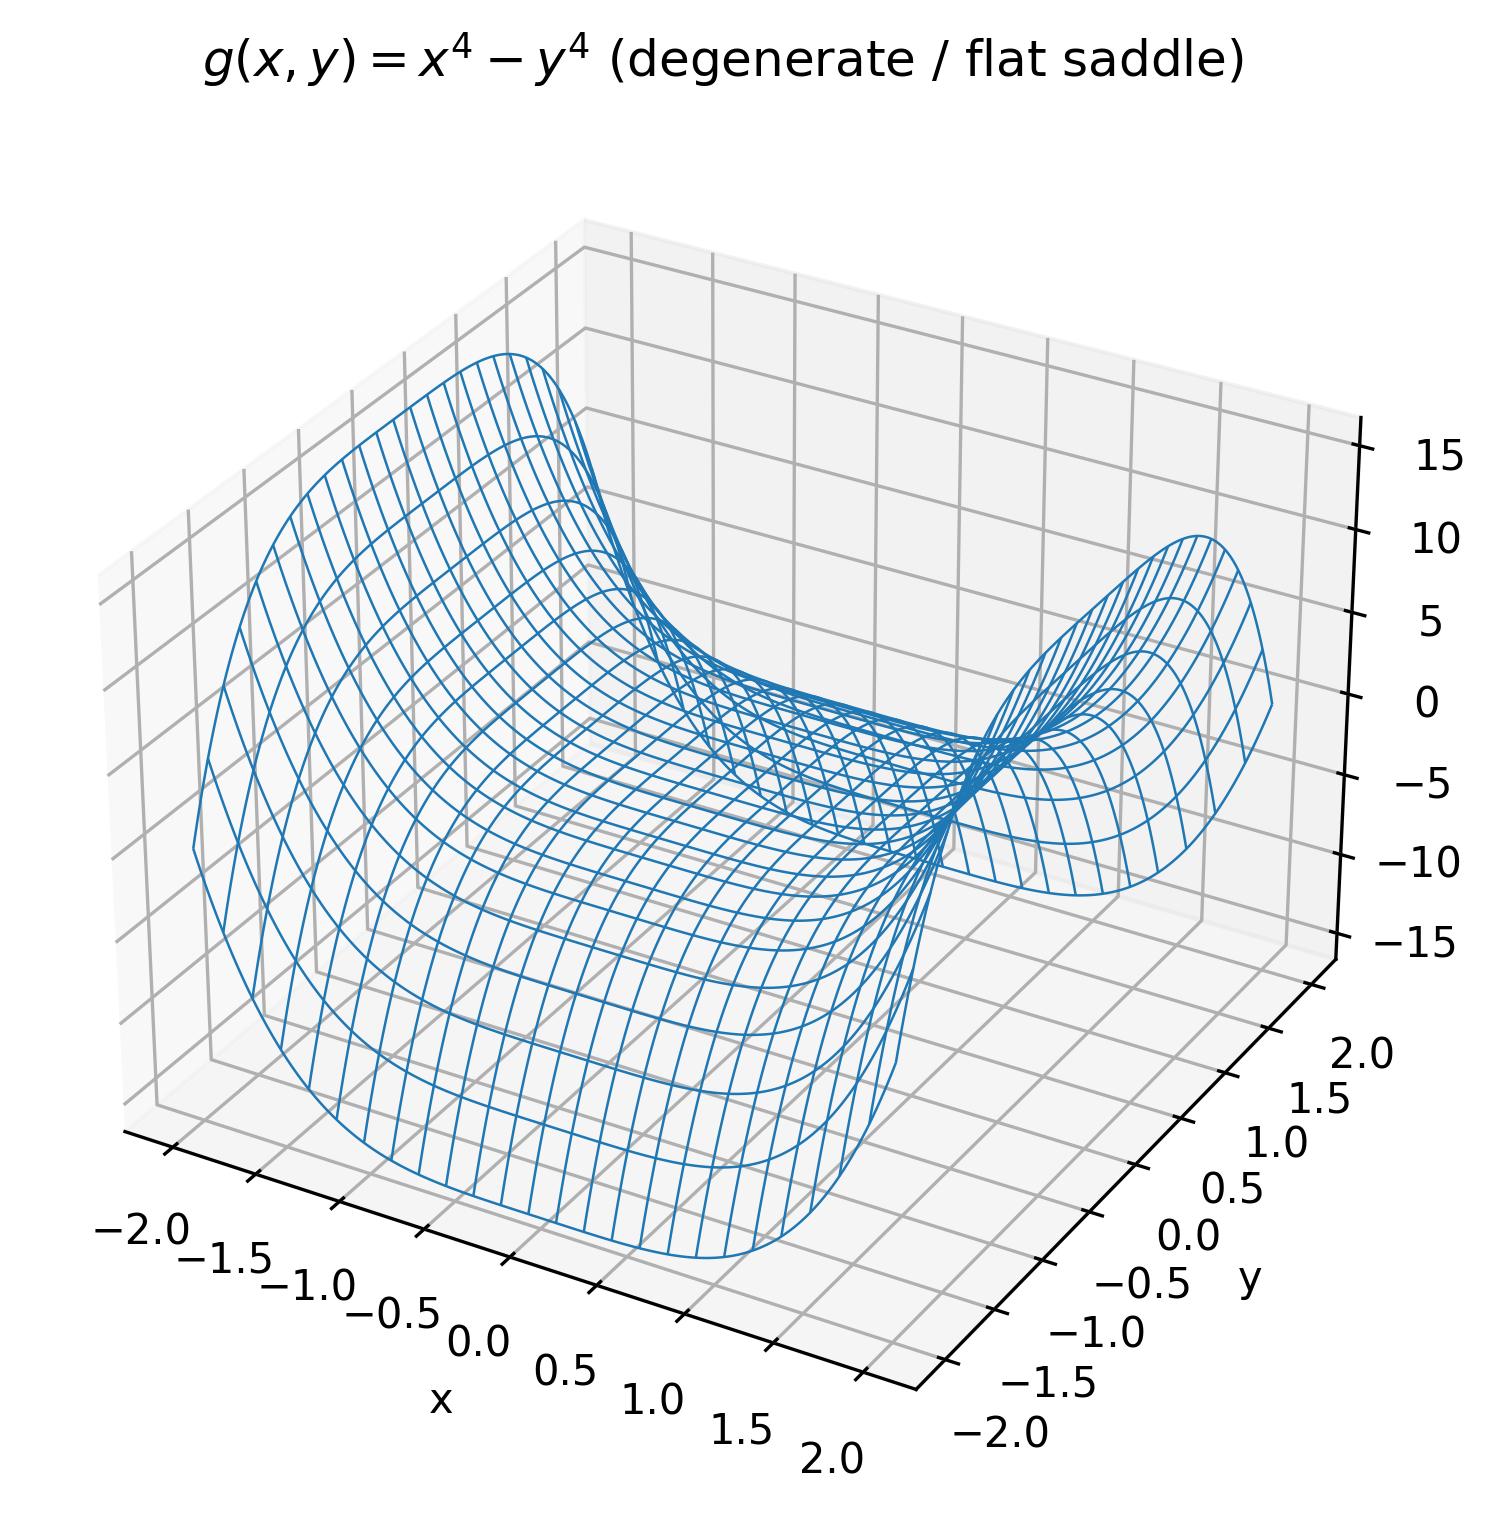
\includegraphics[width=\linewidth]{chapters/part07_volume_vii/figures/fig_saddle_x4_minus_y4_surface.png}
			\caption*{$g(x,y)=x^4-y^4$: 3D surface (degenerate / flat saddle).}
		\end{minipage}\hfill
		\begin{minipage}{0.49\linewidth}
			\centering
			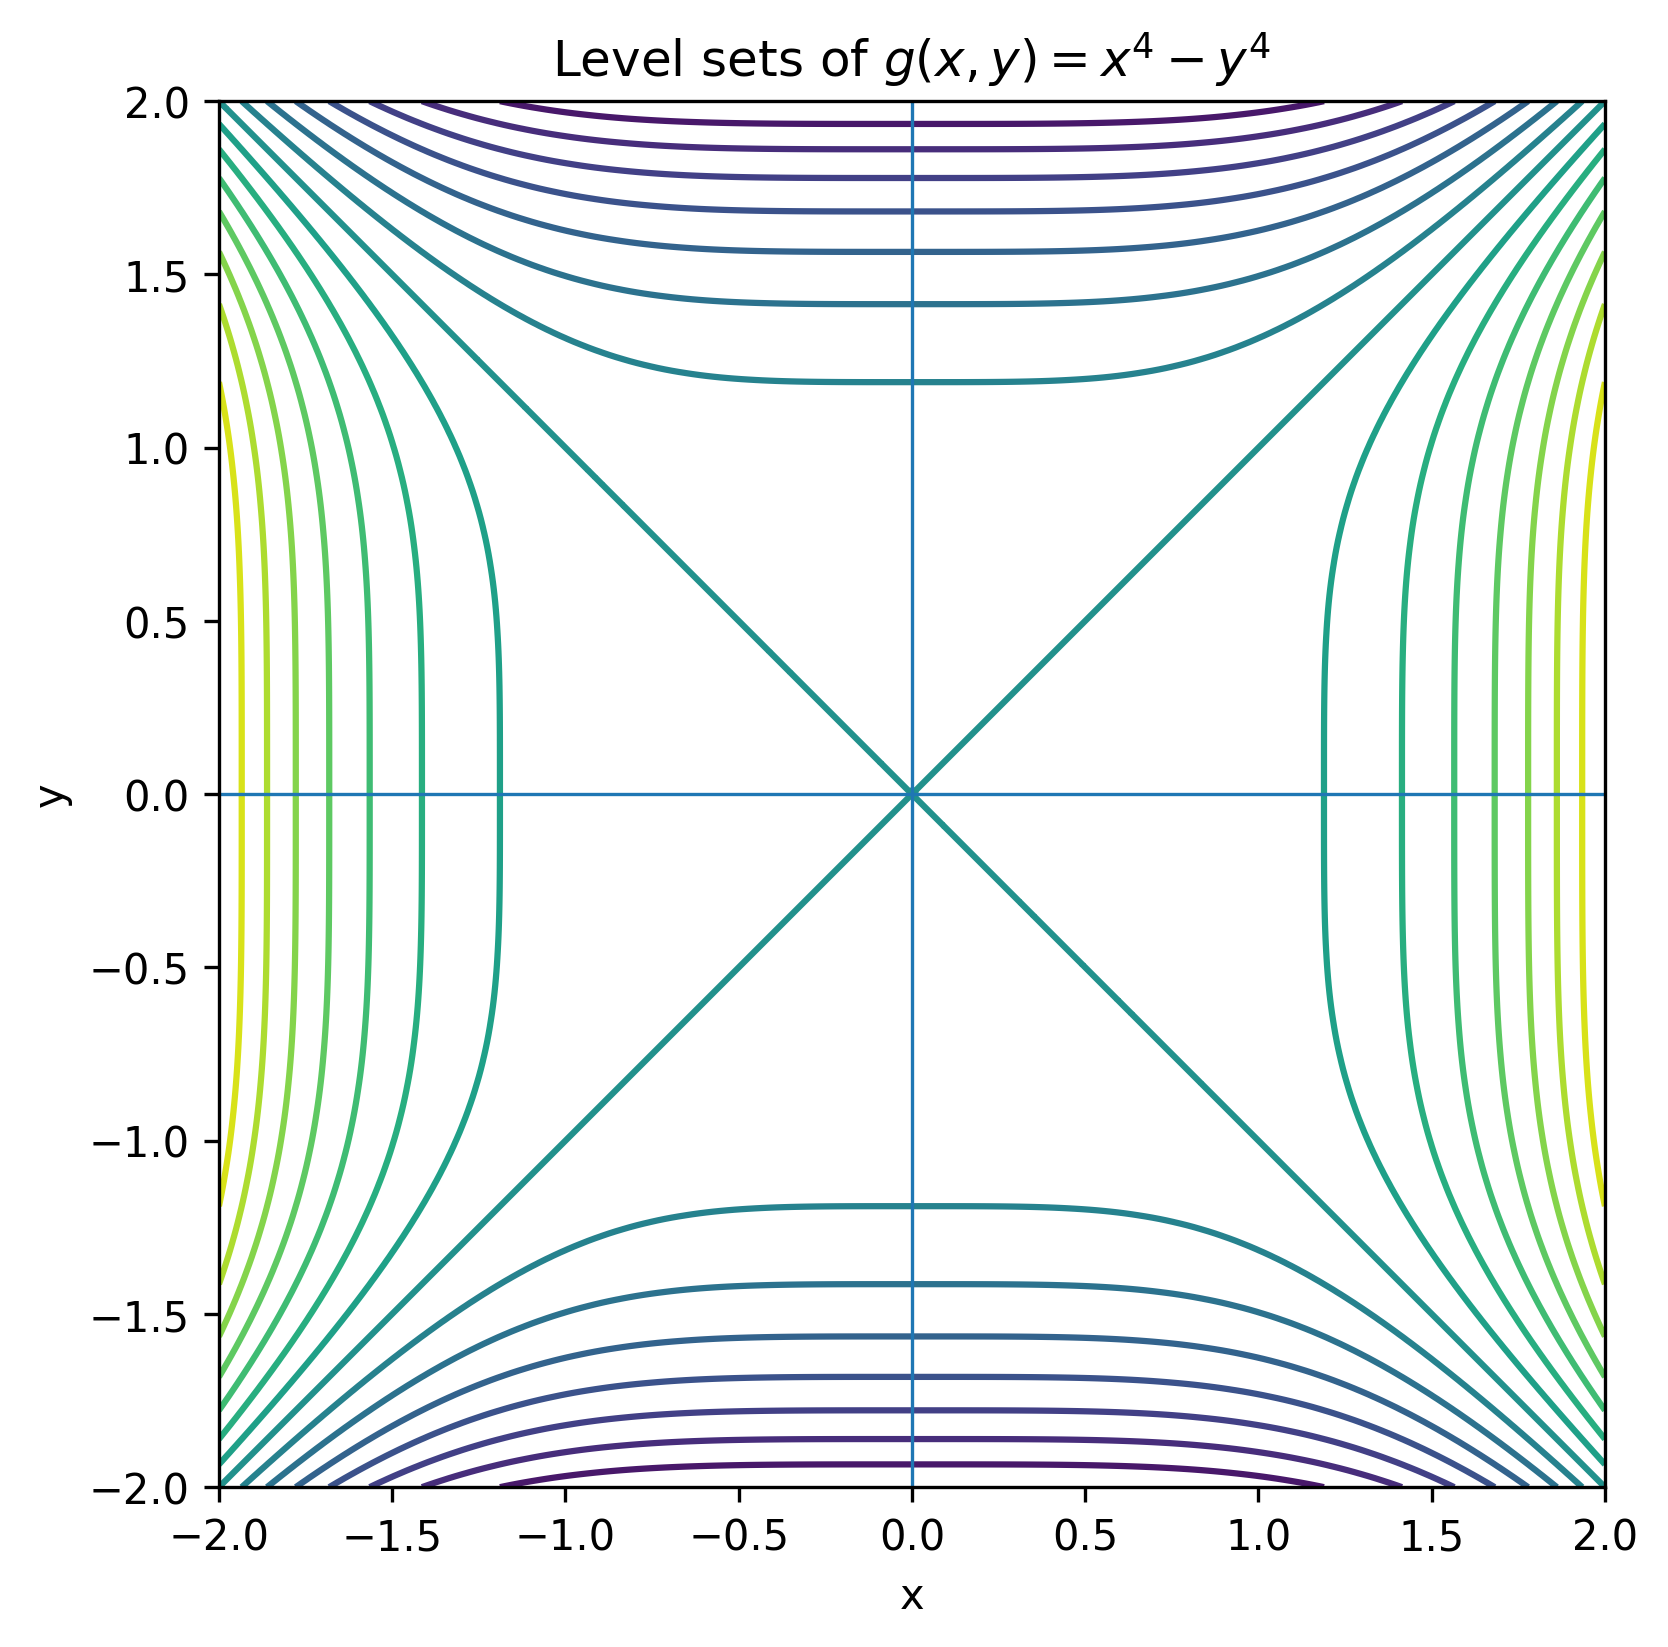
\includegraphics[width=\linewidth]{chapters/part07_volume_vii/figures/fig_saddle_x4_minus_y4_contours.png}
			\caption*{$g(x,y)=x^4-y^4$: level sets.}
		\end{minipage}
		\caption{A degenerate saddle: the quadratic term vanishes (Hessian singular), so the saddle shape appears only in higher order.}
	\end{figure}
	
	\par\medskip\noindent\textbf{Why $d(\det)_A(H)=\mathrm{tr}(\mathrm{adj}(A)^T H)$}\par\smallskip

	
	\noindent
	Let $\det:M(n)\to\mathbb{R}$ be the determinant function. Fix $A\in M(n)$ and a direction $H\in M(n)$.
	Define a one-variable function
	\[
	g(t)=\det(A+tH).
	\]
	By definition of the directional derivative,
	\[
	d(\det)_A(H)=g'(0).
	\]
	
	\medskip
	\noindent\textbf{Step 1: Multilinearity in columns.}
	Write the columns of $A$ as $a_1,\dots,a_n$ and the columns of $H$ as $h_1,\dots,h_n$.
	Then
	\[
	A+tH=[\,a_1+th_1,\ a_2+th_2,\ \dots,\ a_n+th_n\,].
	\]
	Since $\det$ is multilinear in the columns,
	\[
	\det(A+tH)=\det(a_1+th_1,\dots,a_n+th_n)
	\]
	\[
	=\det(a_1,\dots,a_n)
	+t\sum_{j=1}^n \det(a_1,\dots,h_j,\dots,a_n)
	+\text{(terms of order }t^2\text{ and higher)}.
	\]
	Therefore the coefficient of $t$ equals $g'(0)$, and hence
	\[
	d(\det)_A(H)=g'(0)=\sum_{j=1}^n \det(a_1,\dots,h_j,\dots,a_n).
	\tag{$\ast$}
	\]
	
	\medskip
	\noindent\textbf{Step 2: Laplace expansion along the replaced column.}
	Fix an index $j$. Let $B=(a_1,\dots,h_j,\dots,a_n)$ be the matrix obtained by replacing the $j$-th column of $A$ by $h_j$.
	Expand $\det(B)$ along the $j$-th column:
	\[
	\det(B)=\sum_{i=1}^n B_{ij}\,C_{ij}(B),
	\]
	where $C_{ij}(B)=(-1)^{i+j}\det(B_{\widehat{i},\widehat{j}})$ is the $(i,j)$-cofactor.
	Deleting row $i$ and column $j$ removes the replaced column, hence
	\[
	B_{\widehat{i},\widehat{j}}=A_{\widehat{i},\widehat{j}}
	\qquad\Longrightarrow\qquad
	C_{ij}(B)=(-1)^{i+j}\det(A_{\widehat{i},\widehat{j}})=C_{ij}(A).
	\]
	Moreover $B_{ij}=(h_j)_i=H_{ij}$. Therefore
	\[
	\det(a_1,\dots,h_j,\dots,a_n)=\det(B)=\sum_{i=1}^n H_{ij}\,C_{ij}(A).
	\]
	
	\medskip
	\noindent\textbf{Step 3: Sum over all $j$ and identify the adjugate.}
	Substituting the previous formula into $(\ast)$ gives
	\[
	d(\det)_A(H)=\sum_{j=1}^n\sum_{i=1}^n H_{ij}\,C_{ij}(A)
	=\sum_{i,j} C_{ij}(A)\,H_{ij}.
	\]
	Recall that the adjugate matrix satisfies
	\[
	\mathrm{adj}(A)_{ji}=C_{ij}(A)
	\quad\text{(adjugate is the transpose of the cofactor matrix).}
	\]
	Hence
	\[
	\sum_{i,j} C_{ij}(A)\,H_{ij}
	=\sum_{i,j} \mathrm{adj}(A)_{ji}\,H_{ij}.
	\]
	Finally, using the identity
	\[
	\mathrm{tr}(X^T Y)=\sum_{i,j} X_{ij}Y_{ij},
	\]
	we obtain
	\[
	\mathrm{tr}\big(\mathrm{adj}(A)^T H\big)
	=\sum_{i,j} \big(\mathrm{adj}(A)^T\big)_{ij}H_{ij}
	=\sum_{i,j} \mathrm{adj}(A)_{ji}H_{ij}.
	\]
	Therefore,
	\[
	d(\det)_A(H)=\mathrm{tr}\big(\mathrm{adj}(A)^T H\big).
	\]
	
	\par\medskip\noindent\textbf{Why $\det$ is multilinear, and where the $t^2,t^3,\dots$ terms come from}\par\smallskip

	
	\noindent\textbf{Multilinearity (in columns).}
	Write an $n\times n$ matrix by its columns
	\[
	A=[c_1,\dots,c_n],\qquad c_j\in\mathbb{R}^n.
	\]
	A map $F(c_1,\dots,c_n)$ is called \emph{multilinear} if it is linear in each argument separately, i.e.\ for every
	fixed $j$ and all vectors $u,v\in\mathbb{R}^n$ and scalars $\lambda\in\mathbb{R}$,
	\[
	F(c_1,\dots,c_{j-1},u+v,c_{j+1},\dots,c_n)
	=
	F(c_1,\dots,c_{j-1},u,c_{j+1},\dots,c_n)
	+
	F(c_1,\dots,c_{j-1},v,c_{j+1},\dots,c_n),
	\]
	and
	\[
	F(c_1,\dots,c_{j-1},\lambda u,c_{j+1},\dots,c_n)
	=
	\lambda\,F(c_1,\dots,c_{j-1},u,c_{j+1},\dots,c_n).
	\]
	For the determinant, this property follows from the Leibniz formula:
	\[
	\det(A)=\sum_{\sigma\in S_n}\mathrm{sgn}(\sigma)\prod_{i=1}^n a_{i,\sigma(i)}.
	\]
	Fix a column index $j$. In each product $\prod_{i=1}^n a_{i,\sigma(i)}$, the permutation $\sigma$ hits each column
	index exactly once, so \emph{exactly one factor} in the product comes from the $j$-th column. Therefore each summand
	depends linearly on the entries of the $j$-th column, and so does the sum. Since $j$ was arbitrary, $\det$ is linear
	in each column separately, i.e.\ $\det$ is multilinear.
	
	\medskip
	\noindent\textbf{Where the powers $t^2,t^3,\dots$ come from.}
	Let $A,H\in M(n)$ and write their columns as
	\[
	A=[a_1,\dots,a_n],\qquad H=[h_1,\dots,h_n].
	\]
	Then
	\[
	A+tH=[a_1+th_1,\dots,a_n+th_n].
	\]
	Using multilinearity, we can expand $\det(A+tH)$ by distributing over each column (analogous to expanding a product).
	From each column $a_j+th_j$ we choose either $a_j$ or $th_j$. This yields a sum of $2^n$ determinants:
	\[
	\det(A+tH)
	=
	\sum_{S\subset\{1,\dots,n\}}
	\det\big(b_1(S),\dots,b_n(S)\big),
	\]
	where
	\[
	b_j(S)=
	\begin{cases}
		th_j, & j\in S,\\
		a_j, & j\notin S.
	\end{cases}
	\]
	If $|S|=m$, then exactly $m$ columns contribute a factor $t$, and by linearity we can factor these out:
	\[
	\det\big(b_1(S),\dots,b_n(S)\big)
	=
	t^m\,\det\big(c_1(S),\dots,c_n(S)\big),
	\]
	where $c_j(S)=h_j$ if $j\in S$ and $c_j(S)=a_j$ otherwise.
	Hence the expansion groups naturally by the size $m$ of $S$:
	\[
\begin{aligned}
\det(A+tH)
&=\det(A)\\
&\quad
+t\sum_{|S|=1}
\det\!\bigl(\text{replace one column of \(A\) by the corresponding column of \(H\)}\bigr)\\
&\quad+t^2(\cdots)+\cdots+t^n\det(H).
\end{aligned}
\]
	In particular, the terms with $t^2,t^3,\dots$ come from choosing $th_j$ in two, three, $\dots$ columns respectively.
	
	\medskip
	\noindent\textbf{Why only the linear term matters for the derivative at $t=0$.}
	If we write
	\[
	\det(A+tH)=\det(A)+tL+t^2Q(t),
	\]
	then
	\[
	\frac{d}{dt}\Big|_{t=0}\det(A+tH)=L,
	\]
	because $\frac{d}{dt}\big(t^2Q(t)\big)\big|_{t=0}=0$.
	Therefore $d(\det)_A(H)$ is exactly the coefficient of $t$ in the multilinear expansion above.
	
	\par\medskip\noindent\textbf{Directional derivative of $\det$ for $3\times 3$ and $4\times 4$}\par\smallskip

	
	\noindent\textbf{$3\times 3$ case (fully expanded).}
	Let
	\[
	A=\begin{pmatrix}
		a&b&c\\
		d&e&f\\
		g&h&i
	\end{pmatrix},\qquad
	H=\begin{pmatrix}
		p&q&r\\
		s&t&u\\
		v&w&x
	\end{pmatrix}.
	\]
	Writing $A=[a_1,a_2,a_3]$ and $H=[h_1,h_2,h_3]$ by columns, multilinearity gives
	\[
	d(\det)_A(H)=\frac{d}{dt}\Big|_{0}\det(A+tH)
	=\det(h_1,a_2,a_3)+\det(a_1,h_2,a_3)+\det(a_1,a_2,h_3).
	\]
	Expanding each term along its replaced column yields
	\[
	d(\det)_A(H)=\sum_{i=1}^3 C_{i1}(A)H_{i1}+\sum_{i=1}^3 C_{i2}(A)H_{i2}+\sum_{i=1}^3 C_{i3}(A)H_{i3}
	=\sum_{i,j=1}^3 C_{ij}(A)H_{ij}.
	\]
	The cofactors of $A$ are
	\[
	\begin{aligned}
		C_{11}&=ei-fh, & C_{12}&=fg-di, & C_{13}&=dh-eg,\\
		C_{21}&=ch-bi, & C_{22}&=ai-cg, & C_{23}&=bg-ah,\\
		C_{31}&=bf-ce, & C_{32}&=cd-af, & C_{33}&=ae-bd.
	\end{aligned}
	\]
	Hence
	\[
\boxed{
\begin{aligned}
d(\det)_A(H)
&=(ei-fh)p+(fg-di)q+(dh-eg)r\\
&\quad +(ch-bi)s+(ai-cg)t+(bg-ah)u\\
&\quad +(bf-ce)v+(cd-af)w+(ae-bd)x.
\end{aligned}}
\]
	
	\medskip
	\noindent\textbf{$4\times 4$ case (column-replacement formula).}
	Write $A=[a_1,a_2,a_3,a_4]$ and $H=[h_1,h_2,h_3,h_4]$. Then
	\[
	\boxed{
		d(\det)_A(H)=
		\det(h_1,a_2,a_3,a_4)+
		\det(a_1,h_2,a_3,a_4)+
		\det(a_1,a_2,h_3,a_4)+
		\det(a_1,a_2,a_3,h_4).}
	\]
	Equivalently,
	\[
	d(\det)_A(H)=\sum_{i,j=1}^4 C_{ij}(A)H_{ij},
	\qquad
	C_{ij}(A)=(-1)^{i+j}\det(A_{\widehat{i},\widehat{j}}).
	\]
	
	\medskip
	\noindent\textbf{Example (diagonal $A$).}
	If $A=\mathrm{diag}(d_1,d_2,d_3,d_4)$ and $H=(h_{ij})$, then
	\[
	\boxed{
		d(\det)_A(H)=d_2d_3d_4\,h_{11}+d_1d_3d_4\,h_{22}+d_1d_2d_4\,h_{33}+d_1d_2d_3\,h_{44}.}
	\]
	
	\par\medskip\noindent\textbf{Visualizing $\det:M(2)\cong\mathbb{R}^4\to\mathbb{R}$ and its derivative via slices}\par\smallskip

	
	\noindent
	A $2\times 2$ matrix can be parametrized by $(a,b,c,d)\in\mathbb{R}^4$:
	\[
	A=\begin{pmatrix}a&b\\ c&d\end{pmatrix},
	\qquad
	\det(A)=ad-bc.
	\]
	Since the domain is $4$-dimensional, we cannot plot $\det$ directly. Instead, we fix two coordinates and visualize
	$2$-dimensional slices. For example, if $b,c$ are fixed then $\det$ becomes a function of $(a,d)$:
	\[
	\det(A)=ad-(bc),
	\]
	so its level sets in the $(a,d)$-plane are hyperbolas. Similarly, if $a,d$ are fixed then
	\[
	\det(A)=(ad)-bc,
	\]
	and level sets in the $(b,c)$-plane are again hyperbolas. To visualize the \emph{derivative} on a slice, we plot the
	gradient vector field of the sliced function (arrows give the direction of steepest increase \emph{within the slice}).
	
	\medskip
	\noindent\textbf{Figures (determinant slices).}
	\begin{figure}[htbp]
		\centering
		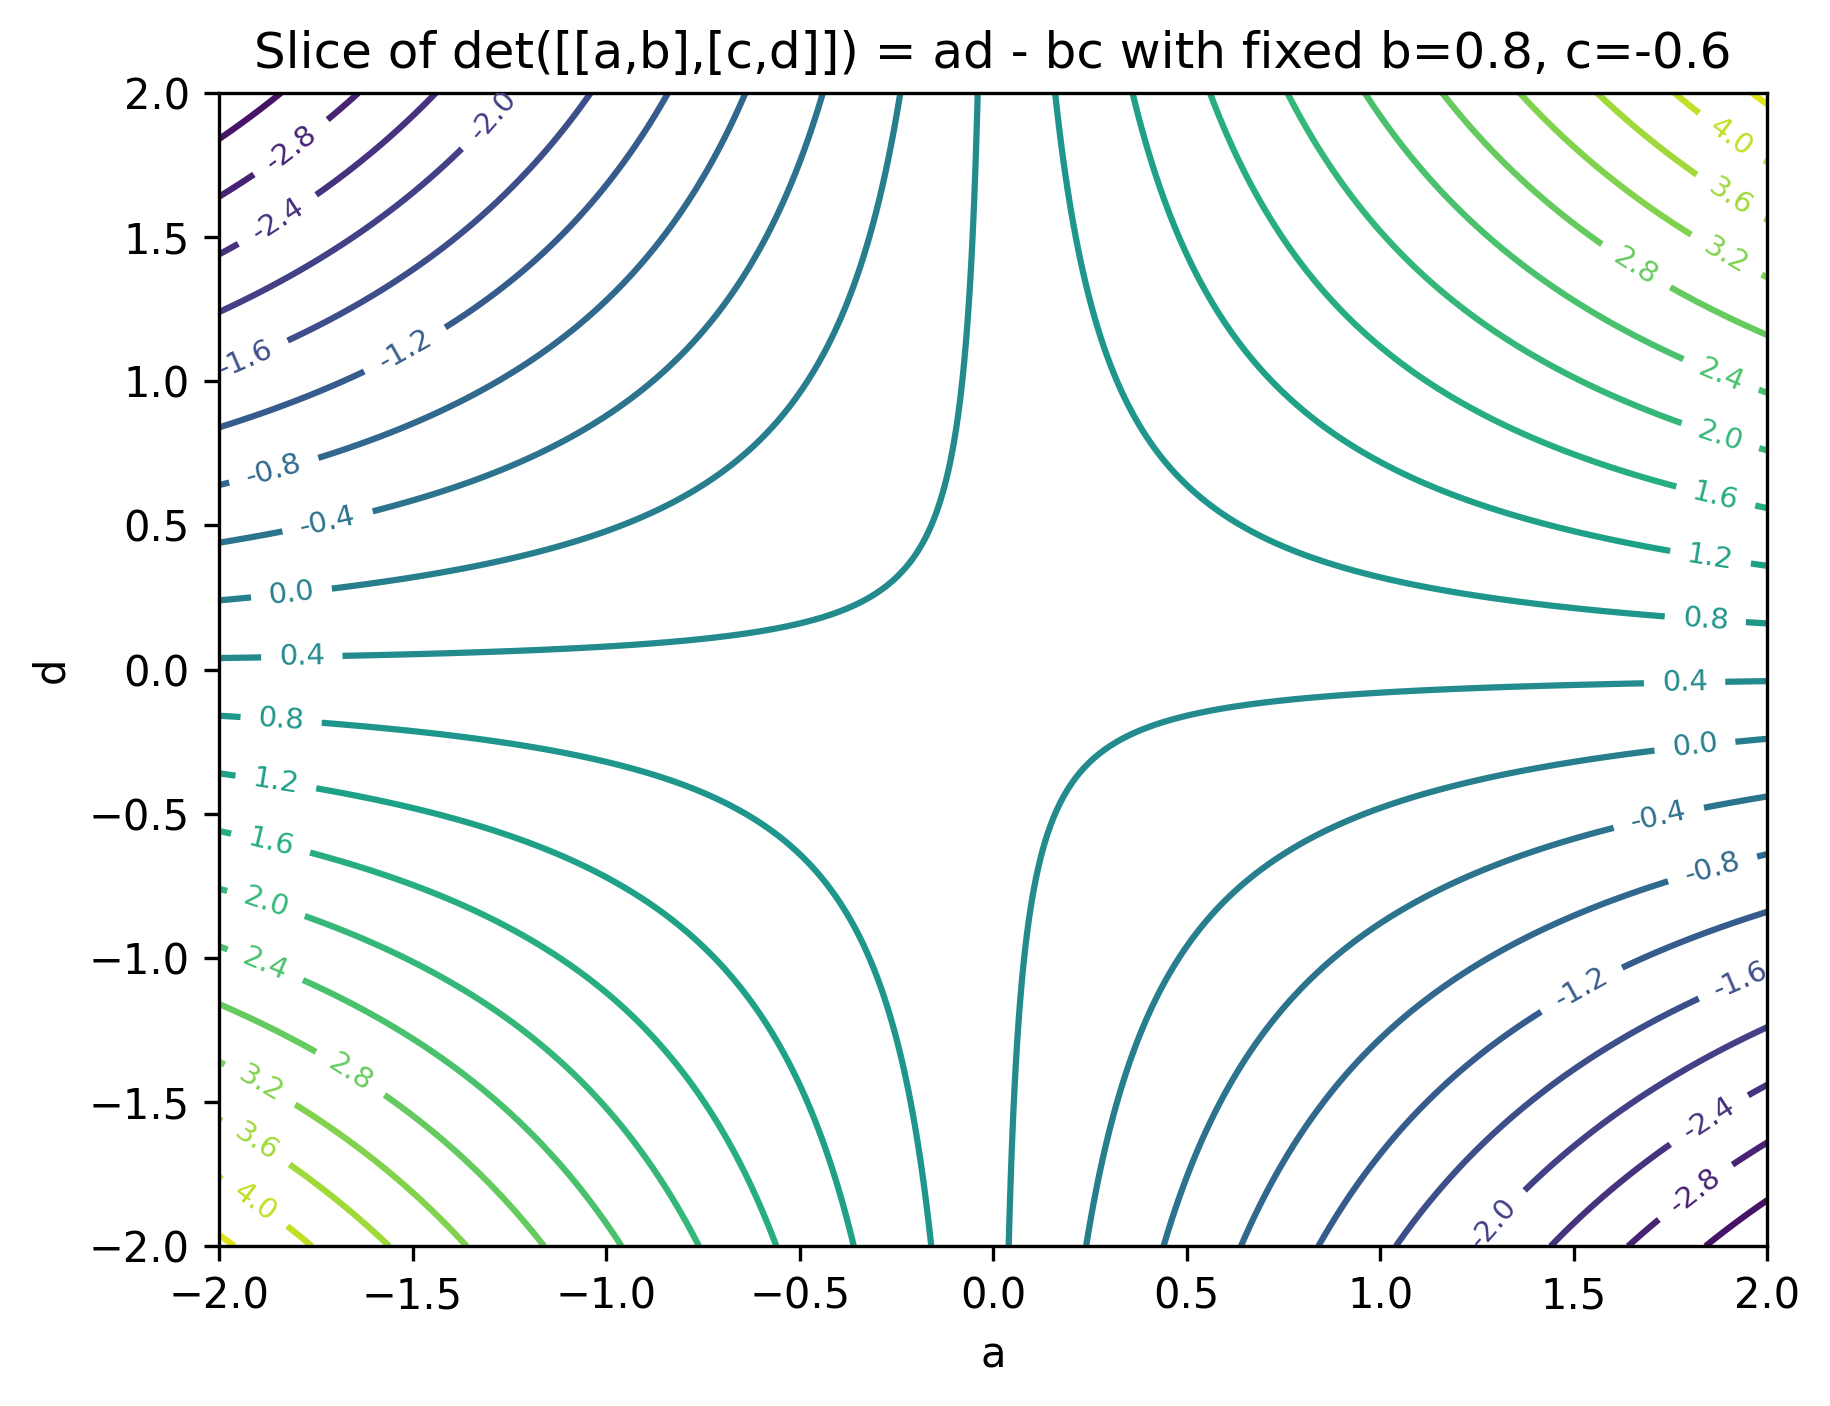
\includegraphics[width=0.78\linewidth]{chapters/part07_volume_vii/figures/det_R4_to_R_slice_contours_ad_fixed_bc.png}
		\caption{Contour plot of the slice with fixed $b,c$: $\det=ad-bc$ as a function of $(a,d)$.}
	\end{figure}
	
	\begin{figure}[htbp]
		\centering
		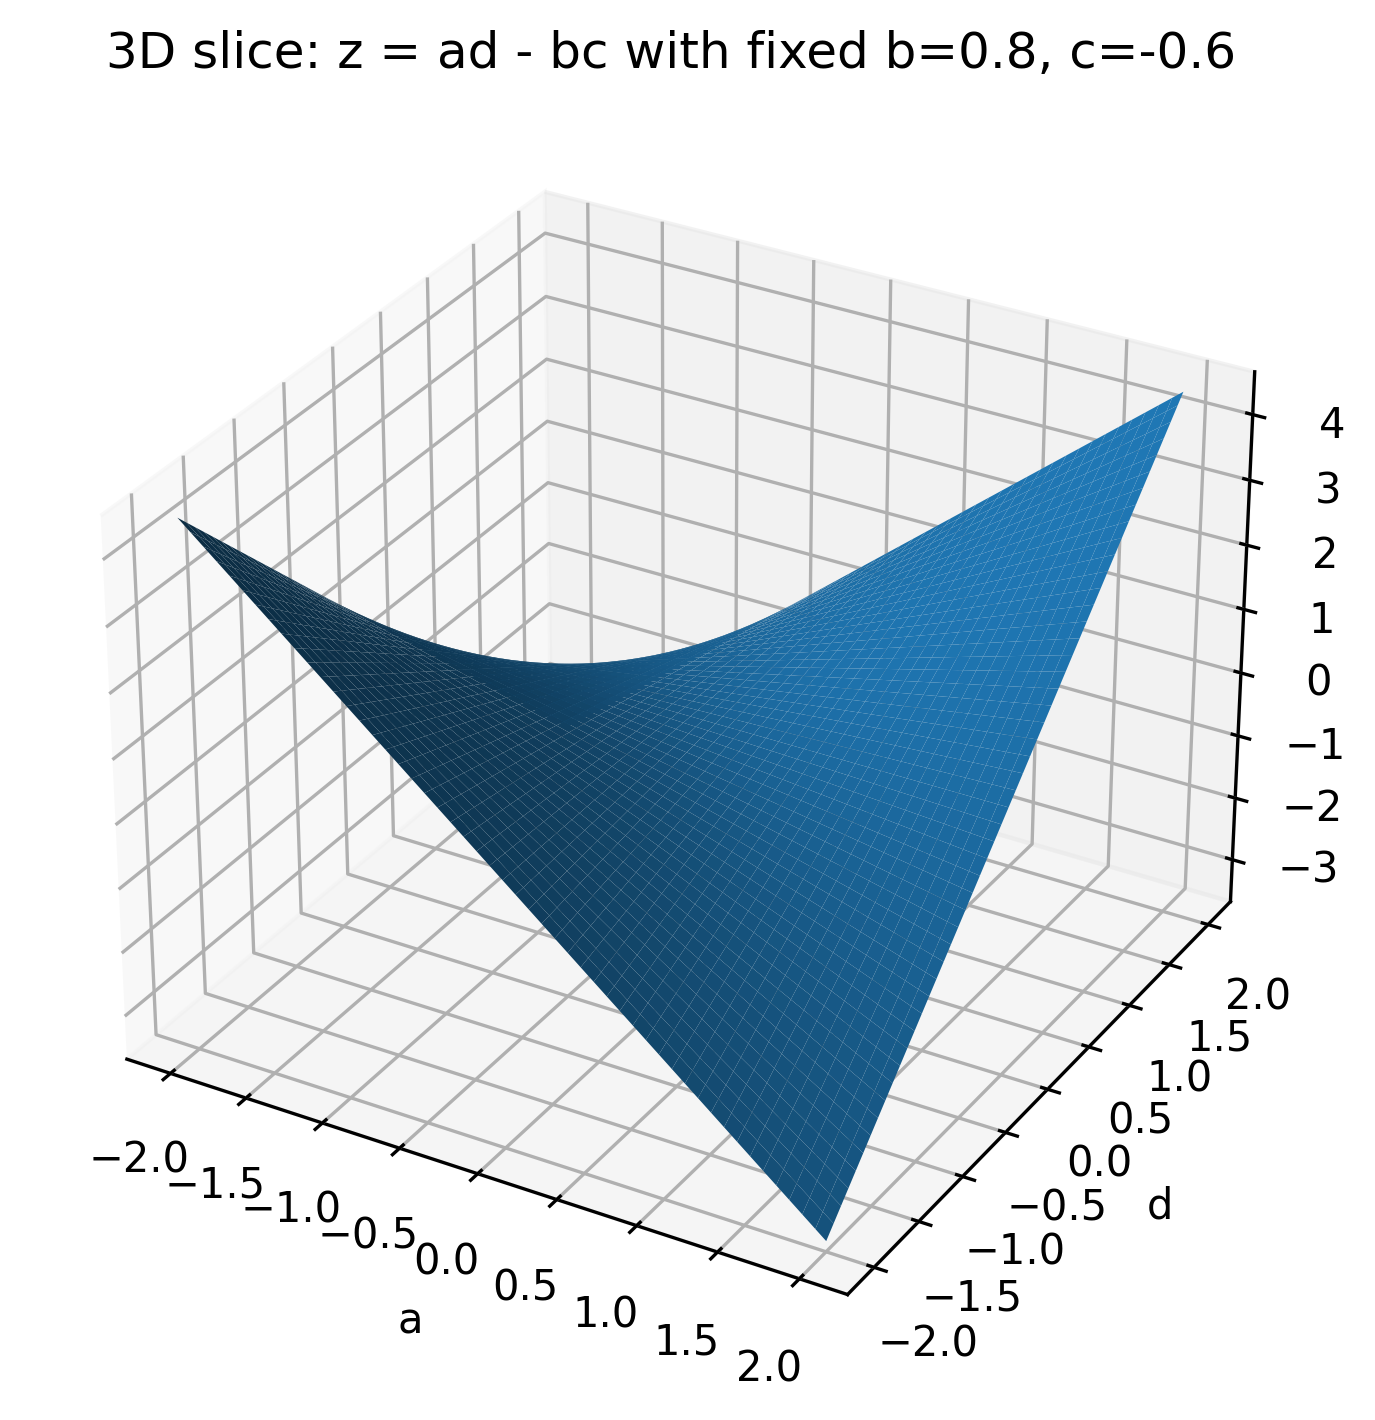
\includegraphics[width=0.78\linewidth]{chapters/part07_volume_vii/figures/det_R4_to_R_slice_surface_ad_fixed_bc.png}
		\caption{3D surface slice (fixed $b,c$): $z=\det(a,d)=ad-bc$, a saddle shifted by $-bc$.}
	\end{figure}
	
	\begin{figure}[htbp]
		\centering
		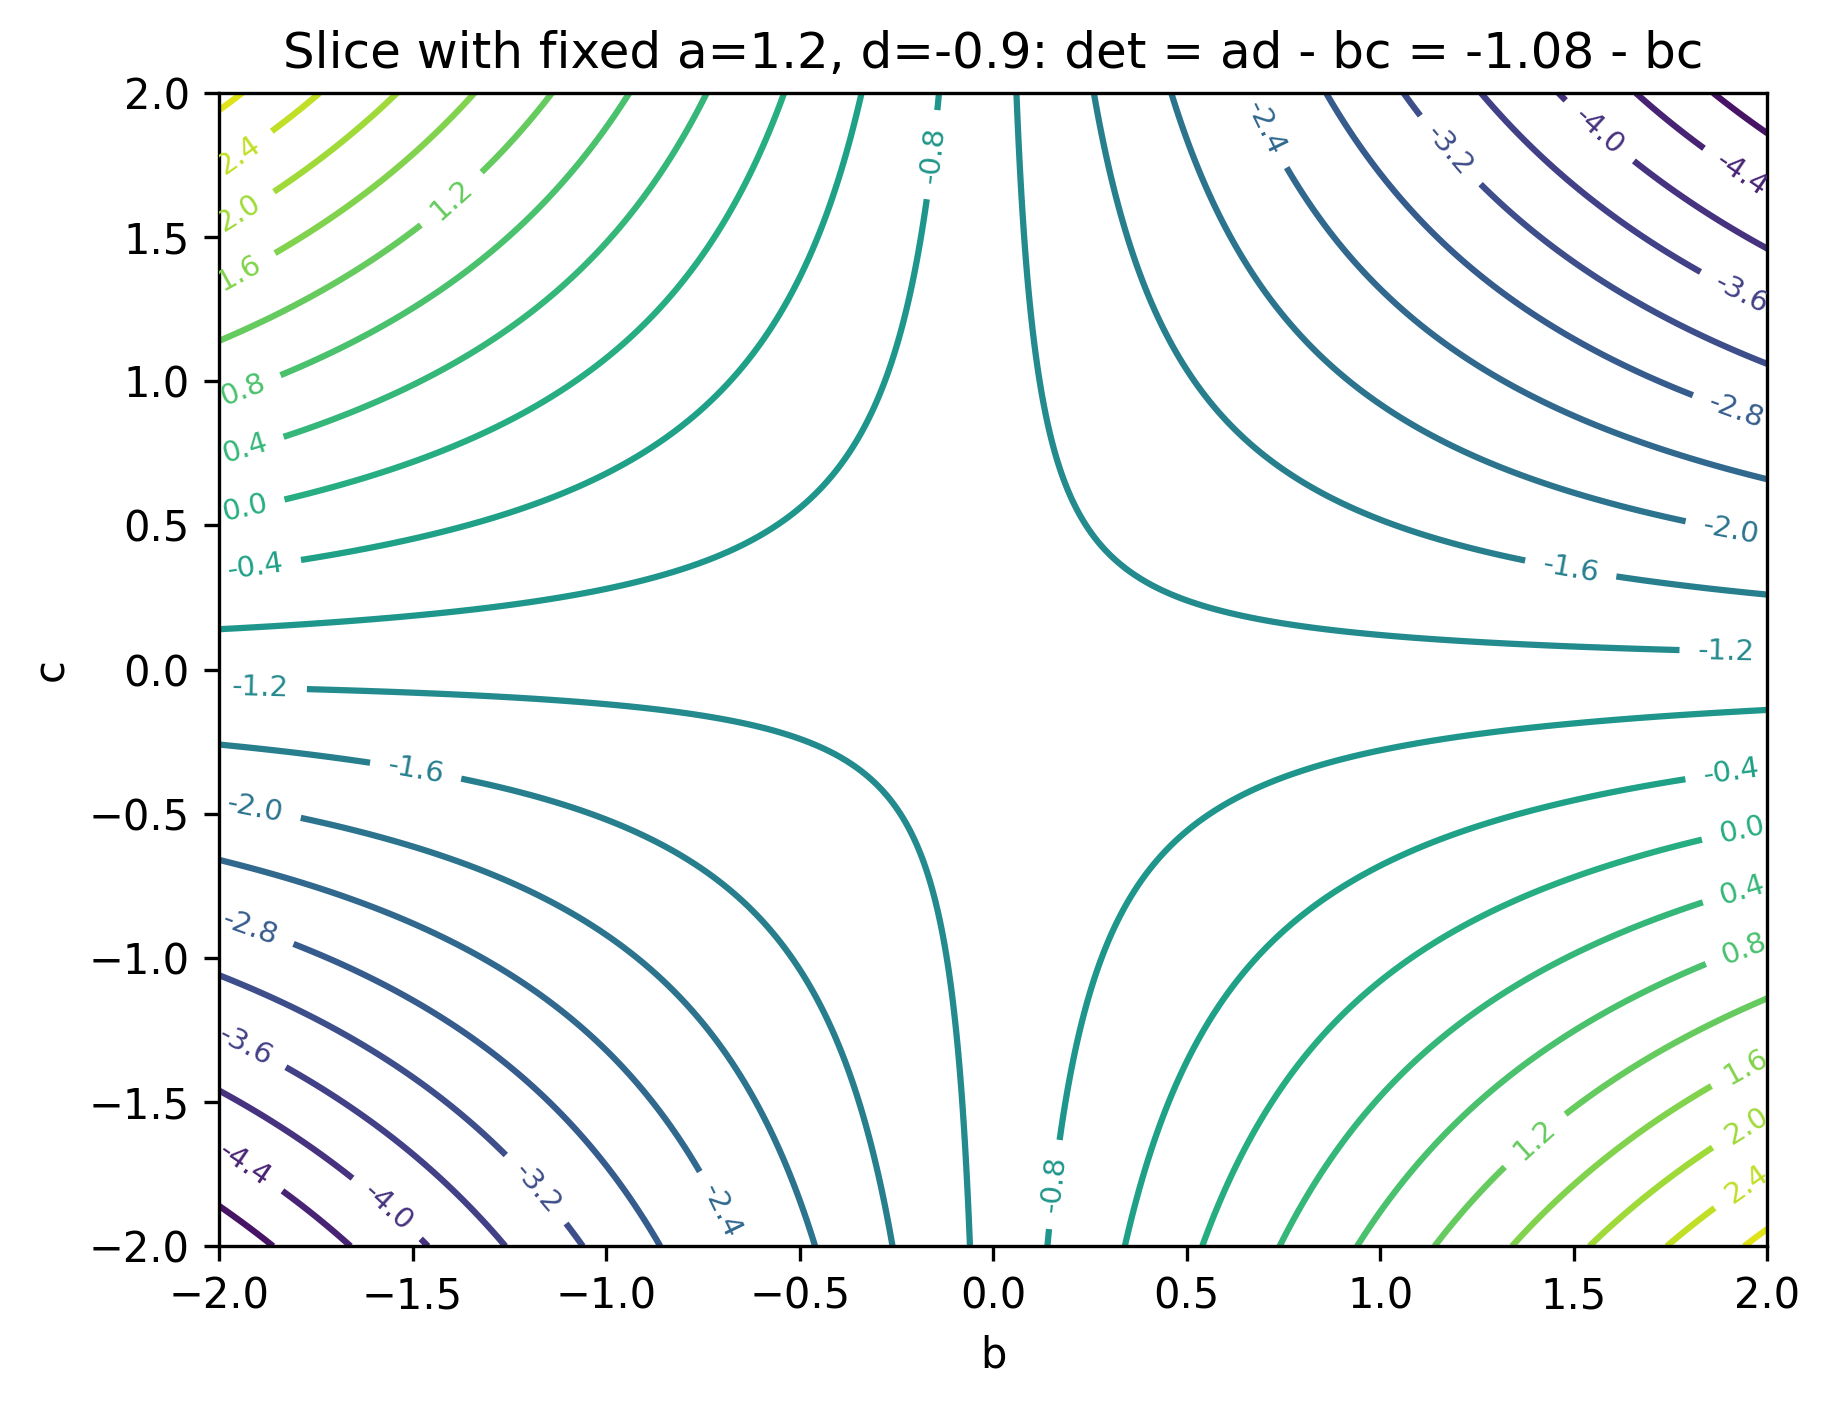
\includegraphics[width=0.78\linewidth]{chapters/part07_volume_vii/figures/det_R4_to_R_slice_contours_bc_fixed_ad.png}
		\caption{Contour plot of the slice with fixed $a,d$: $\det=ad-bc$ as a function of $(b,c)$.}
	\end{figure}
	
	\medskip
	\noindent\textbf{Figures (derivative on slices).}
	\noindent
	On the $(a,d)$-slice (with fixed $b,c$), the sliced function is $F(a,d)=ad-(bc)$, hence
	\[
	\nabla_{(a,d)}F(a,d)=(\partial_a F,\partial_d F)=(d,a).
	\]
	On the $(b,c)$-slice (with fixed $a,d$), the sliced function is $G(b,c)=(ad)-bc$, hence
	\[
	\nabla_{(b,c)}G(b,c)=(\partial_b G,\partial_c G)=(-c,-b).
	\]
	
	\begin{figure}[htbp]
		\centering
		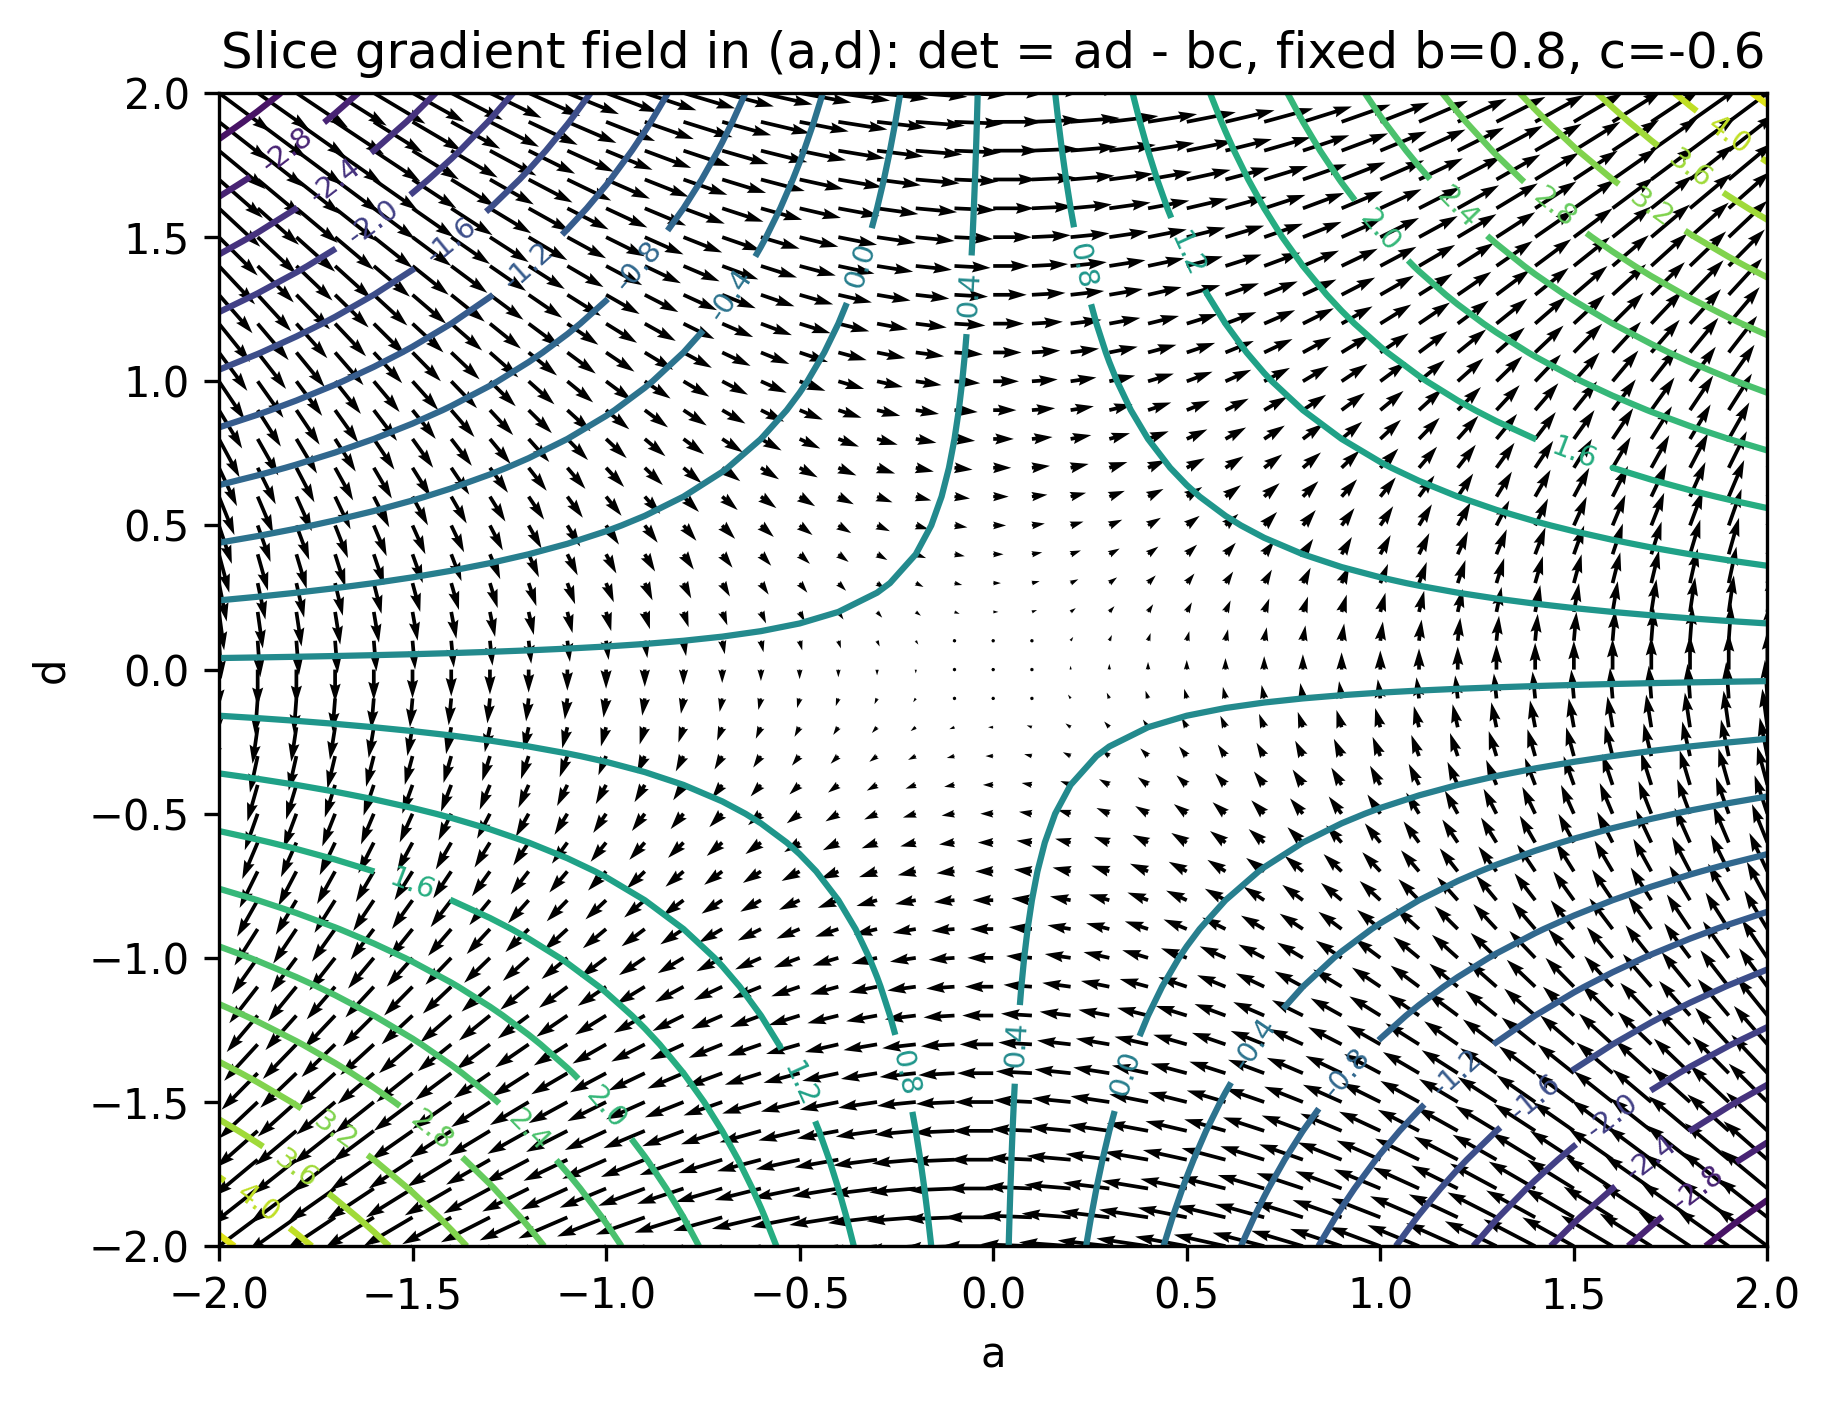
\includegraphics[width=0.78\linewidth]{chapters/part07_volume_vii/figures/det_slice_gradfield_ad_fixed_bc.png}
		\caption{Gradient field on the $(a,d)$-slice (fixed $b,c$). Arrows show $\nabla_{(a,d)}(ad-bc)=(d,a)$.}
	\end{figure}
	
	\begin{figure}[htbp]
		\centering
		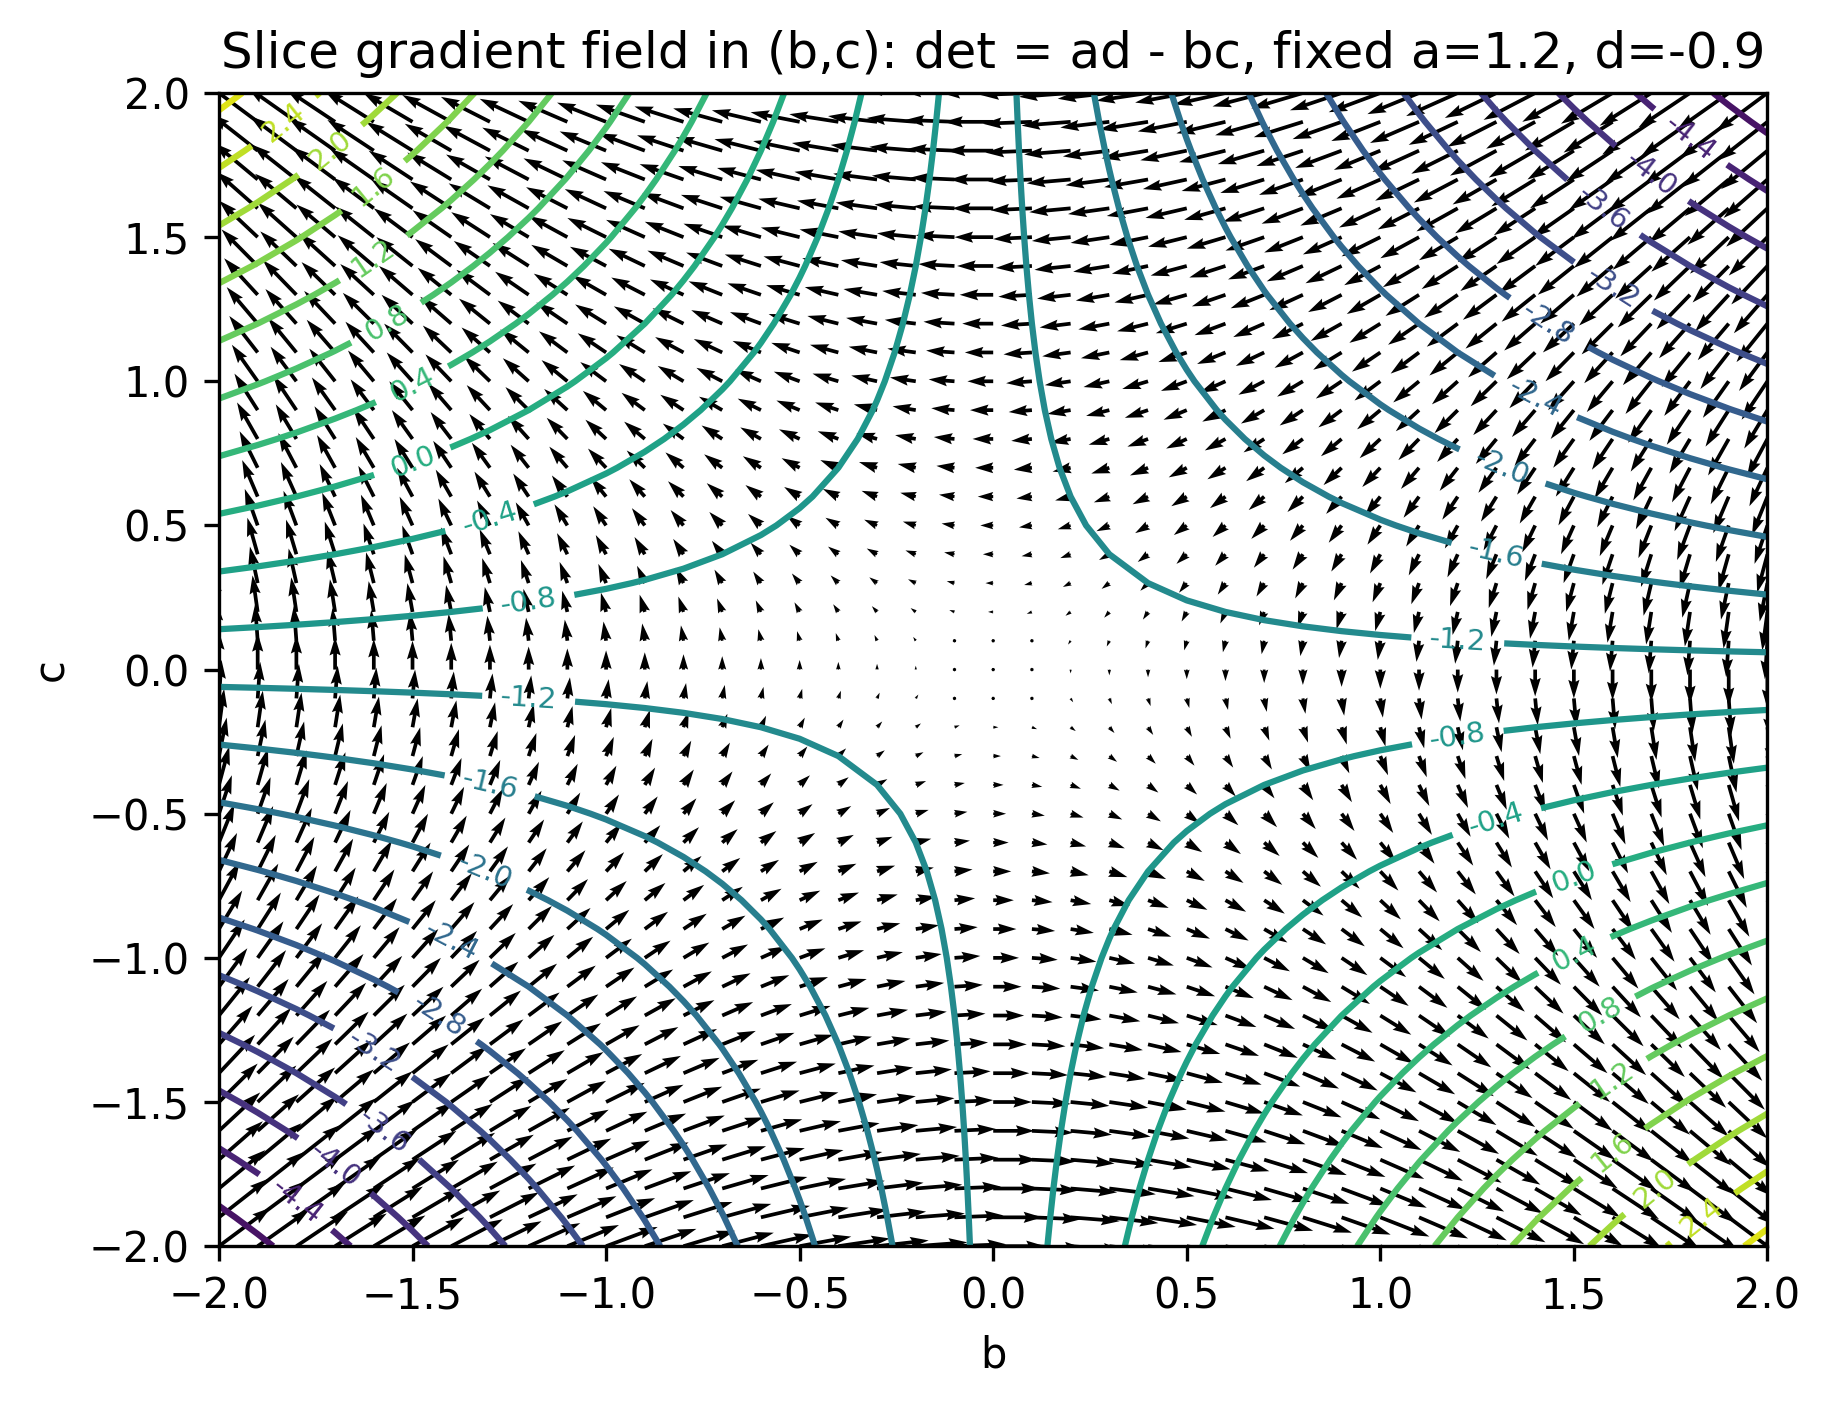
\includegraphics[width=0.78\linewidth]{chapters/part07_volume_vii/figures/det_slice_gradfield_bc_fixed_ad.png}
		\caption{Gradient field on the $(b,c)$-slice (fixed $a,d$). Arrows show $\nabla_{(b,c)}(ad-bc)=(-c,-b)$.}
	\end{figure}
	
	\par\medskip\noindent\textbf{Gradient vs.\ derivative on a slice of $\det$}\par\smallskip

	
	\noindent
	Identify $M(2)\cong\mathbb{R}^4$ via coordinates $(a,b,c,d)$:
	\[
	F(a,b,c,d)=\det\!\begin{pmatrix}a&b\\ c&d\end{pmatrix}=ad-bc.
	\]
	Since $F$ has a $4$-dimensional domain, we visualize it by fixing two variables and taking a $2$-dimensional slice.
	Fix $b,c\in\mathbb{R}$. Then the restricted (slice) function is
	\[
	f_{b,c}(a,d):=F(a,b,c,d)=ad-bc,
	\qquad (a,d)\in\mathbb{R}^2.
	\]
	
	\medskip
	\noindent\textbf{Derivative (differential) on the slice.}
	The derivative of $f_{b,c}$ at a point $(a,d)$ is the linear map
	\[
	df_{b,c}\big|_{(a,d)}:\mathbb{R}^2\to\mathbb{R},
	\]
	defined by
	\[
	df_{b,c}\big|_{(a,d)}(\Delta a,\Delta d)
	=\frac{\partial f_{b,c}}{\partial a}(a,d)\,\Delta a
	+\frac{\partial f_{b,c}}{\partial d}(a,d)\,\Delta d.
	\]
	For $f_{b,c}(a,d)=ad-bc$ we have
	\[
	\frac{\partial f_{b,c}}{\partial a}(a,d)=d,
	\qquad
	\frac{\partial f_{b,c}}{\partial d}(a,d)=a,
	\]
	hence
	\[
	\boxed{
		df_{b,c}\big|_{(a,d)}(\Delta a,\Delta d)=d\,\Delta a+a\,\Delta d.}
	\]
	
	\medskip
	\noindent\textbf{Gradient as a representation of the derivative.}
	In $\mathbb{R}^2$ with the standard dot product, the differential can be written as
	\[
	df_{b,c}\big|_{(a,d)}(\Delta a,\Delta d)=\nabla f_{b,c}(a,d)\cdot(\Delta a,\Delta d),
	\]
	so the gradient vector is
	\[
	\boxed{\nabla f_{b,c}(a,d)=\big(d,a\big).}
	\]
	Therefore, the arrow field in the figure is a visualization of the derivative:
	each arrow at $(a,d)$ points in the direction of fastest increase of $f_{b,c}$ within the $(a,d)$-slice.
	
	\medskip
	\noindent\textbf{Full $4$-dimensional derivative (for completeness).}
	For $F(a,b,c,d)=ad-bc$,
	\[
	\nabla F(a,b,c,d)=\big(d,-c,-b,a\big),
	\]
	and the differential at $(a,b,c,d)$ is the linear map
	\[
	\boxed{
		dF\big|_{(a,b,c,d)}(\Delta a,\Delta b,\Delta c,\Delta d)
		=d\,\Delta a-c\,\Delta b-b\,\Delta c+a\,\Delta d.}
	\]
	The $(a,d)$-slice figure corresponds to restricting this differential to variations with $\Delta b=\Delta c=0$.
	
	\par\medskip\noindent\textbf{Why $df_{(a,d)}(\Delta a,\Delta d)=\nabla f(a,d)\cdot(\Delta a,\Delta d)$?}\par\smallskip

	
	Let $f:\mathbb{R}^2\to\mathbb{R}$ be differentiable and let $p=(a,d)$.
	The \emph{differential} of $f$ at $p$ is the linear map (a linear functional)
	\[
	df_p:\mathbb{R}^2\to\mathbb{R}
	\]
	characterized by the first--order Taylor approximation
	\[
	f(p+h)=f(p)+df_p(h)+o(\|h\|)\qquad (h\to 0).
	\]
	Writing $h=(\Delta a,\Delta d)$ and using partial derivatives, one obtains the explicit formula
	\[
	df_{(a,d)}(\Delta a,\Delta d)=
	\frac{\partial f}{\partial x}(a,d)\,\Delta a
	+\frac{\partial f}{\partial y}(a,d)\,\Delta d.
	\]
	
	Now introduce the \emph{gradient} (with respect to the standard dot product on $\mathbb{R}^2$)
	\[
	\nabla f(a,d)=\left(\frac{\partial f}{\partial x}(a,d),\ \frac{\partial f}{\partial y}(a,d)\right).
	\]
	Then the same expression can be rewritten as a dot product:
	\[
	\frac{\partial f}{\partial x}(a,d)\,\Delta a
	+\frac{\partial f}{\partial y}(a,d)\,\Delta d
	=
	\left(\frac{\partial f}{\partial x}(a,d),\frac{\partial f}{\partial y}(a,d)\right)\cdot(\Delta a,\Delta d)
	=
	\nabla f(a,d)\cdot(\Delta a,\Delta d).
	\]
	Hence
	\[
	df_{(a,d)}(\Delta a,\Delta d)=\nabla f(a,d)\cdot(\Delta a,\Delta d).
	\]
	
	\medskip
	\noindent\textbf{Conceptual reason.}
	The differential $df_p$ is a covector (linear functional). In Euclidean space with the standard inner product
	$\langle\cdot,\cdot\rangle$, every covector $L$ can be represented uniquely as
	\[
	L(h)=\langle v,h\rangle
	\quad\text{for a unique vector }v.
	\]
	The gradient is precisely this representing vector: it is defined by
	\[
	df_p(h)=\langle \nabla f(p),h\rangle\qquad\text{for all }h\in\mathbb{R}^2.
	\]
	For the standard inner product, $\langle u,v\rangle=u\cdot v$, giving the stated formula.

\end{solution}

\subsection*{Main-text correspondence: VII/04}

\begin{problem}[CP-VII-0013 --- Problem 9 (Differentials of multiplication and inversion; sign in the right-invariant bracket)]
\label{prob:cp-vii-0013}
For a Lie group $G$ compute the derivatives $D_{(e,e)}m:\mathfrak g\oplus\mathfrak g\to\mathfrak g$ and
$D_e i:\mathfrak g\to\mathfrak g$ of the multiplication and inversion maps $m$ and $i$ at the identity.
Show that $i_*$ exchanges left-invariant and right-invariant vector fields, and deduce that the bracket operation
on $\mathfrak g$ defined using right-invariant (rather than left-invariant) vector fields differs from the usual one by a sign.
\end{problem}

\begin{solution}
Let $m(g,h)=gh$ and $i(g)=g^{-1}$.

\emph{Multiplication at $(e,e)$.}
Take curves $g(t),h(t)$ with $g(0)=h(0)=e$ and $g'(0)=X$, $h'(0)=Y$. Then
\[
D_{(e,e)}m(X,Y)=\frac{d}{dt}\Big|_{0}g(t)h(t)=X+Y.
\]

\emph{Inversion at $e$.}
Using $g(t)=\exp(tX)$ gives $i(g(t))=\exp(-tX)$, hence
\[
D_e i(X)=\frac{d}{dt}\Big|_{0}\exp(-tX)=-X.
\]

\emph{$i_*$ exchanges left- and right-invariant fields.}
For $X\in\mathfrak g$ define $X^L(g)=(dL_g)_eX$ and $X^R(g)=(dR_g)_eX$.
The identity
\[
i\circ L_g = R_{g^{-1}}\circ i
\]
implies, upon differentiation at $e$,
\[
(d i)_g\circ(dL_g)_e=(dR_{g^{-1}})_e\circ(d i)_e=-(dR_{g^{-1}})_e.
\]
Thus, at $g^{-1}=i(g)$,
\[
(i_*X^L)_{g^{-1}}=(d i)_g(X^L_g)=-(dR_{g^{-1}})_eX=-(X^R)_{g^{-1}}.
\]
So inversion sends left-invariant fields to (minus) right-invariant ones (and similarly in the other direction).

\emph{Sign in the right-invariant bracket.}
Pushforwards preserve Lie brackets: $i_*[U,V]=[i_*U,i_*V]$. Apply this to $U=X^L$, $V=Y^L$ and evaluate at $e$:
\[
(d i)_e([X^L,Y^L]_e)=[i_*X^L,i_*Y^L]_e=[-X^R,-Y^R]_e=[X^R,Y^R]_e.
\]
Since $(d i)_e=-\mathrm{Id}$, we get
\[
[X^R,Y^R]_e=-[X^L,Y^L]_e.
\]
Hence defining $[X,Y]_{\mathrm{right}}:=[X^R,Y^R]_e$ yields
\[
[X,Y]_{\mathrm{right}}=-[X,Y]_{\mathrm{usual}}.
\]

\par\medskip\noindent\textbf{Theory for Problem 9 (Lie group actions, orbits, quotients)}\par\smallskip


\textbf{Smooth action.}
A smooth (left) action of a Lie group $G$ on a manifold $M$ is a smooth map
$\alpha:G\times M\to M$, $(g,p)\mapsto g\cdot p$ with $e\cdot p=p$ and
$g\cdot(h\cdot p)=(gh)\cdot p$.

\textbf{Orbit and stabilizer.}
The orbit of $p$ is $\mathcal O_p=G\cdot p=\{g\cdot p:g\in G\}$.
The stabilizer is $G_p=\{g\in G:g\cdot p=p\}$, a Lie subgroup.

\textbf{Infinitesimal action.}
For $X\in\mathfrak g=T_eG$ define the fundamental vector field
\[
X_M(p)=\left.\frac{d}{dt}\right|_0 \big(\exp(tX)\cdot p\big).
\]
Then $T_p\mathcal O_p=\{X_M(p):X\in\mathfrak g\}$ and (up to sign convention)
$[X_M,Y_M]=\pm [X,Y]_M$.

\textbf{Quotients.}
If the action is free and proper, then $M/G$ is a smooth manifold and the projection
$\pi:M\to M/G$ is a submersion; $M\to M/G$ is a principal $G$-bundle.
\end{solution}

\begin{problem}[CP-VII-0014 --- Problem 10 (Morphisms intertwine exponentials and induce Lie algebra homomorphisms)]
\label{prob:cp-vii-0014}
Let $F:H\to G$ be a morphism of Lie groups, i.e.\ a smooth map which is a group homomorphism.
Show that
\[
F(\exp_H(\xi))=\exp_G(D_eF(\xi))\quad\text{for all }\xi\in\mathfrak h,
\]
and deduce that $D_eF$ is a Lie algebra homomorphism, i.e.\ a linear map which respects the bracket operation.
This shows, in particular, that if $H$ is an embedded Lie subgroup of $G$ then the exponential map and bracket
on $\mathfrak h$ are the restrictions of those on $\mathfrak g$.
\end{problem}

\begin{solution}
Fix $\xi\in\mathfrak h$. The curve $\gamma(t)=\exp_H(t\xi)$ is a one-parameter subgroup of $H$.
Since $F$ is a group homomorphism, $F\circ\gamma$ is a one-parameter subgroup of $G$.
Its derivative at $0$ is
\[
\frac{d}{dt}\Big|_{0}F(\exp_H(t\xi))=(D_eF)(\xi)\in\mathfrak g.
\]
A one-parameter subgroup in $G$ is uniquely determined by its tangent at $t=0$, and equals
$t\mapsto \exp_G(tX)$ where $X$ is that tangent. Therefore for all $t$,
\[
F(\exp_H(t\xi))=\exp_G(t\,D_eF(\xi)).
\]
Setting $t=1$ gives $F(\exp_H(\xi))=\exp_G(D_eF(\xi))$.

To show $D_eF$ preserves brackets, let $\xi,\eta\in\mathfrak h$ and let $\xi^L,\eta^L$ be the corresponding
left-invariant vector fields on $H$. The identity $F\circ L_h=L_{F(h)}\circ F$ implies
\[
F_*(\xi^L)=(D_eF(\xi))^L,\qquad F_*(\eta^L)=(D_eF(\eta))^L.
\]
Naturality of brackets under pushforward gives
\[
F_*[\xi^L,\eta^L]=[F_*\xi^L,F_*\eta^L].
\]
Evaluating at $e$ yields
\[
D_eF([\xi,\eta])=[D_eF(\xi),D_eF(\eta)],
\]
so $D_eF:\mathfrak h\to\mathfrak g$ is a Lie algebra homomorphism.

If $H\subset G$ is an embedded Lie subgroup and $F$ is the inclusion, then $\exp_H$ and the bracket on
$\mathfrak h$ are the restrictions of $\exp_G$ and the bracket on $\mathfrak g$.

\par\medskip\noindent\textbf{Theory for Problem 10 (left-invariant fields, exponential, Ad)}\par\smallskip


\textbf{Left-invariant fields and Lie algebra.}
A vector field $X$ on $G$ is left-invariant if $(dL_g)_h(X_h)=X_{gh}$ for all $g,h$.
Evaluation at $e$ identifies left-invariant fields with $\mathfrak g=T_eG$.
The bracket of left-invariant fields induces the Lie bracket on $\mathfrak g$.

\textbf{Exponential map.}
For each $X\in\mathfrak g$ there is a unique one-parameter subgroup $\gamma_X:\mathbb R\to G$
with $\gamma_X'(0)=X$. Define $\exp(X)=\gamma_X(1)$.
Then $\exp(tX)=\gamma_X(t)$ and $d(\exp)_0=\mathrm{id}$.

\textbf{Adjoint representation.}
Conjugation $C_g(h)=ghg^{-1}$ gives $\mathrm{Ad}_g=(dC_g)_e:\mathfrak g\to\mathfrak g$.
Differentiating yields $\mathrm{ad}_X(Y)=\left.\frac{d}{dt}\right|_0\mathrm{Ad}_{\exp(tX)}Y$,
and $\mathrm{ad}_X(Y)=[X,Y]$.
Moreover $g\exp(X)g^{-1}=\exp(\mathrm{Ad}_g X)$.
\end{solution}

\begin{problem}[CP-VII-0015 --- Problem 1 --- Properness of standard Lie group actions]
\label{prob:cp-vii-0015}
Show that the following Lie group actions are proper.
\begin{enumerate}
	\item The action of $\mathbb{K}^\times$ on $\mathbb{K}^{n+1}\setminus\{0\}$ by rescaling, where $\mathbb{K}$ is $\mathbb{R}$ or $\mathbb{C}$.
	\item The right- (or left-) translation action of an embedded Lie subgroup $H\subset G$ on $G$.
	\item Any action of a compact group.
\end{enumerate}
\end{problem}

\begin{solution}
Recall: an action $G\times M\to M$ is proper if the map
\[
\Phi: G\times M \longrightarrow M\times M,
\qquad
(g,x)\longmapsto (g\cdot x,\;x)
\]
is a proper map (preimages of compact sets are compact). On manifolds, this is equivalent to the sequential criterion:
\[
\Phi(g_i,x_i)\to (y,x)
\quad\Longrightarrow\quad
(g_i,x_i)\ \text{has a convergent subsequence.}
\]

\textbf{(a) Rescaling action of $\mathbb{K}^\times$ on $\mathbb{K}^{n+1}\setminus\{0\}$.}
Let
\[
(\lambda_i,x_i)\in \mathbb{K}^\times \times \bigl(\mathbb{K}^{n+1}\setminus\{0\}\bigr)
\]
be such that
\[
(\lambda_i x_i,\;x_i)\longrightarrow (y,x)
\qquad\text{in}\qquad
\bigl(\mathbb{K}^{n+1}\setminus\{0\}\bigr)\times\bigl(\mathbb{K}^{n+1}\setminus\{0\}\bigr).
\]
Then
\[
x_i\to x\neq 0.
\]
Choose an index $j$ such that $x^{(j)}\neq 0$. For $i$ large, $x_i^{(j)}\neq 0$, and
\[
\lambda_i
=
\frac{(\lambda_i x_i)^{(j)}}{x_i^{(j)}}
\longrightarrow
\frac{y^{(j)}}{x^{(j)}}
=:\lambda
\in \mathbb{K}^\times.
\]

Hence
\[
\lambda_i\to \lambda
\qquad\text{and}\qquad
x_i\to x,
\]
so
\[
(\lambda_i,x_i)\to (\lambda,x).
\]
Therefore the action is proper.

\textbf{(b) Translation action of an embedded Lie subgroup $H\subset G$ on $G$.}
Consider the right translation action
\[
H\times G\longrightarrow G,
\qquad
(h,g)\longmapsto g h.
\]
Assume
\[
(g_i h_i,\;g_i)\longrightarrow (g',g)
\qquad\text{in}\qquad
G\times G.
\]
Then
\[
g_i\to g
\qquad\text{and}\qquad
g_i h_i\to g',
\]
so
\[
h_i
=
g_i^{-1}(g_i h_i)
\longrightarrow
g^{-1}g'
=:h.
\]
Since $H$ is embedded (in particular, closed in $G$), the limit satisfies
\[
h\in H.
\]
Hence $(h_i,g_i)$ converges (after passing to a subsequence if desired), so the action is proper. (The left action is analogous.)

\textbf{(c) Any action of a compact group.}
Let a compact Lie group $K$ act on $M$. Suppose
\[
(k_i\cdot x_i,\;x_i)\longrightarrow (y,x).
\]
Then
\[
x_i\to x.
\]
By compactness, $(k_i)$ has a convergent subsequence
\[
k_{i_m}\to k\in K.
\]
Thus
\[
(k_{i_m},x_{i_m})\to (k,x),
\]
so the action is proper.
\end{solution}

\begin{problem}[CP-VII-0016 --- Problem 10: Derivations at a point and the tangent space]
\label{prob:cp-vii-0016}
\noindent Fix a smooth manifold $X$ and a point $p\in X$. Let $\mathcal{O}_{X,p}$ be the space of germs
of smooth functions about $p$; this is an $\mathbb{R}$-vector space by scalar multiplication.
An $\mathbb{R}$-linear derivation $\mathcal{O}_{X,p}\to\mathbb{R}$ is an $\mathbb{R}$-linear map $d$ such that
\[
d(fg)\;=\; d(f)\,g(p) + f(p)\,d(g)
\qquad\text{for all germs } f,g.
\]
These form an $\mathbb{R}$-vector space denoted $\mathrm{Der}_{\mathbb{R}}(\mathcal{O}_{X,p},\mathbb{R})$.
Show that this vector space is naturally isomorphic to the tangent space $T_pX$.




\end{problem}

\begin{solution}
Let $X$ be a smooth manifold and $p\in X$. Let $\mathcal{O}_{X,p}$ denote the $\mathbb{R}$-algebra of germs
of smooth functions at $p$. An $\mathbb{R}$-linear derivation is an $\mathbb{R}$-linear map
$d:\mathcal{O}_{X,p}\to \mathbb{R}$ such that
\[
d(fg)=d(f)\,g(p)+f(p)\,d(g).
\]
We construct a natural isomorphism
\[
\mathrm{Der}_{\mathbb{R}}(\mathcal{O}_{X,p},\mathbb{R}) \cong T_pX.
\]

\par\medskip\noindent\textbf{Step 1: $T_pX \to \mathrm{Der}_{\mathbb{R}}(\mathcal{O}_{X,p},\mathbb{R})$.}\par\smallskip

Given $v\in T_pX$, define $d_v:\mathcal{O}_{X,p}\to \mathbb{R}$ by
\[
d_v([f]) := (df)_p(v).
\]
This is well-defined on germs, $\mathbb{R}$-linear, and satisfies the Leibniz rule since
\[
d_v(fg) = v(fg) = v(f)\,g(p) + f(p)\,v(g).
\]
Thus we obtain a linear map
\[
\Phi:T_pX\to \mathrm{Der}_{\mathbb{R}}(\mathcal{O}_{X,p},\mathbb{R}),\qquad \Phi(v)=d_v.
\]

\par\medskip\noindent\textbf{Step 2: Derivations kill $\mathfrak{m}_p^2$.}\par\smallskip

Let $\mathfrak{m}_p=\{f\in \mathcal{O}_{X,p}: f(p)=0\}$ be the maximal ideal.
If $g,h\in \mathfrak{m}_p$, then $g(p)=h(p)=0$, so by Leibniz
\[
d(gh)=d(g)\,h(p)+g(p)\,d(h)=0.
\]
Hence every derivation vanishes on $\mathfrak{m}_p^2$.

\par\medskip\noindent\textbf{Step 3: Local coordinate description.}\par\smallskip

Choose a chart $(U,x^1,\dots,x^n)$ around $p$, and assume (after translation) that $x^i(p)=0$.
Given $d\in \mathrm{Der}_{\mathbb{R}}(\mathcal{O}_{X,p},\mathbb{R})$, set
\[
a^i := d(x^i)\in \mathbb{R}.
\]
For any $f\in\mathcal{O}_{X,p}$, write a first-order Taylor expansion in coordinates:
\[
f(x)=f(p)+\sum_{i=1}^n \frac{\partial f}{\partial x^i}(p)\,x^i + \sum_{i,j} x^i x^j\,h_{ij}(x),
\]
where the $h_{ij}$ are smooth. The remainder term lies in $\mathfrak{m}_p^2$, hence is killed by $d$.
Therefore,
\[
d(f)= d\!\left(\sum_{i=1}^n \frac{\partial f}{\partial x^i}(p)\,x^i\right)
=\sum_{i=1}^n \frac{\partial f}{\partial x^i}(p)\,d(x^i)
=\sum_{i=1}^n a^i\,\frac{\partial f}{\partial x^i}(p).
\]

\par\medskip\noindent\textbf{Step 4: Construct the inverse and conclude.}\par\smallskip

Define
\[
v_d := \sum_{i=1}^n a^i\,\frac{\partial}{\partial x^i}\Big|_p \in T_pX.
\]
Then for all $f$,
\[
(df)_p(v_d)=\sum_{i=1}^n a^i\,\frac{\partial f}{\partial x^i}(p)=d(f),
\]
so $d=\Phi(v_d)$. Hence $\Phi$ is surjective. If $\Phi(v)=0$, then $v(x^i)=0$ for all $i$,
so $v=0$, hence $\Phi$ is injective. Therefore $\Phi$ is an isomorphism.

Finally, the map $v\mapsto (f\mapsto (df)_p(v))$ is intrinsic and does not depend on the choice of chart,
so the isomorphism is natural. Consequently,
\[
\mathrm{Der}_{\mathbb{R}}(\mathcal{O}_{X,p},\mathbb{R}) \cong T_pX.
\]


% ------------------------------------------------------------
% Theory for Problem 10
% ------------------------------------------------------------
\par\medskip\noindent\textbf{Theory for Problem 10: Derivations of germs and the tangent space}\par\smallskip


\par\medskip\noindent\textbf{(10.1) Germs and the maximal ideal.}\par\smallskip

Let $\mathcal{O}_{X,p}$ be the $\mathbb{R}$-algebra of germs of smooth functions at $p$.
There is an evaluation map
\[
\mathrm{ev}_p:\mathcal{O}_{X,p}\to \mathbb{R},\qquad [f]\mapsto f(p).
\]
Its kernel is the maximal ideal
\[
\mathfrak{m}_p \;=\; \{\,f\in \mathcal{O}_{X,p}:\ f(p)=0\,\}.
\]

\par\medskip\noindent\textbf{(10.2) Derivations and the Leibniz rule.}\par\smallskip

An $\mathbb{R}$-linear derivation is an $\mathbb{R}$-linear map $d:\mathcal{O}_{X,p}\to \mathbb{R}$ such that
\[
d(fg)=d(f)\,g(p)+f(p)\,d(g)
\]
for all germs $f,g$. Immediate consequences include $d(1)=0$. Moreover, if $f,g\in \mathfrak{m}_p$ then
$f(p)=g(p)=0$ and hence $d(fg)=0$. Thus every derivation kills $\mathfrak{m}_p^2$, and therefore factors as
\[
\mathfrak{m}_p \twoheadrightarrow \mathfrak{m}_p/\mathfrak{m}_p^2 \xrightarrow{\;\;\bar d\;\;} \mathbb{R}.
\]
In particular,
\[
\mathrm{Der}_{\mathbb{R}}(\mathcal{O}_{X,p},\mathbb{R})
\;\cong\;
\mathrm{Hom}_{\mathbb{R}}\bigl(\mathfrak{m}_p/\mathfrak{m}_p^2,\mathbb{R}\bigr).
\]
The quotient $\mathfrak{m}_p/\mathfrak{m}_p^2$ is the (algebraic) cotangent space $T_p^*X$,
and its dual is the tangent space $T_pX$.

\par\medskip\noindent\textbf{(10.3) Tangent vectors as directional derivatives.}\par\smallskip

A tangent vector $v\in T_pX$ defines a derivation by directional differentiation:
\[
d_v([f]) \;:=\; v(f) \;=\; \left.\frac{d}{dt}\right|_{t=0} (f\circ \gamma)(t),
\]
where $\gamma$ is any smooth curve with $\gamma(0)=p$ and $\gamma'(0)=v$.
This satisfies the Leibniz rule, hence gives a map
\[
T_pX \longrightarrow \mathrm{Der}_{\mathbb{R}}(\mathcal{O}_{X,p},\mathbb{R}),\qquad v\mapsto d_v.
\]
Conversely, in local coordinates $(x^1,\dots,x^n)$ near $p$, any derivation $d$ is determined by the scalars
$a^i:=d(x^i)$, since $d$ depends only on the first-order Taylor part (it vanishes on $\mathfrak{m}_p^2$).
Thus, in coordinates,
\[
d \;=\; \sum_{i=1}^n a^i \frac{\partial}{\partial x^i}\Big|_p,
\]
which identifies derivations with tangent vectors and yields the natural isomorphism
\[
\mathrm{Der}_{\mathbb{R}}(\mathcal{O}_{X,p},\mathbb{R}) \;\cong\; T_pX.
\]
	
	
	
	
	% Problem 1
\end{solution}

\subsection*{Main-text correspondence: VII/05}

\begin{problem}[CP-VII-0017 --- Cotangent coordinates and pullback of a covector]
\label{prob:cp-vii-0017}
Let \(M\) be a smooth \(n\)-manifold, \(p\in M\), and
\((x^1,\ldots,x^n)\) a coordinate system near \(p\).

\begin{enumerate}
\item Prove that
\[
dx^1|_p,\ldots,dx^n|_p
\]
form a basis of the cotangent space \(T_p^*M\), dual to
\[
\left.\frac{\partial}{\partial x^1}\right|_p,\ldots,
\left.\frac{\partial}{\partial x^n}\right|_p .
\]
\item If \(F:M\to N\) is smooth and
\[
\eta=\sum_{\alpha=1}^m a_\alpha\,dy^\alpha|_{F(p)}
\in T_{F(p)}^*N,
\]
show that
\[
F_p^*\eta
=
\sum_{i=1}^n
\left(
\sum_{\alpha=1}^m
a_\alpha
\frac{\partial (y^\alpha\circ F)}{\partial x^i}(p)
\right)
dx^i|_p .
\]
\end{enumerate}
\end{problem}

\begin{solution}
By definition,
\[
dx^i|_p(v)=v(x^i).
\]
For the coordinate tangent vectors,
\[
dx^i|_p\!\left(
\left.\frac{\partial}{\partial x^j}\right|_p
\right)
=
\frac{\partial x^i}{\partial x^j}(p)
=
\delta^i_j.
\]
Thus the \(dx^i|_p\) form the basis dual to the coordinate basis of
\(T_pM\).

For the pullback,
\[
(F_p^*\eta)(v)=\eta(dF_pv).
\]
Writing
\[
dF_p\!\left(\frac{\partial}{\partial x^i}\right)
=
\sum_{\alpha=1}^m
\frac{\partial(y^\alpha\circ F)}{\partial x^i}(p)
\frac{\partial}{\partial y^\alpha},
\]
we obtain
\[
(F_p^*\eta)\!\left(\frac{\partial}{\partial x^i}\right)
=
\sum_{\alpha=1}^m
a_\alpha
\frac{\partial(y^\alpha\circ F)}{\partial x^i}(p).
\]
Expanding in the dual basis \(dx^i|_p\) gives the stated formula.
\end{solution}

\subsection*{Main-text correspondence: VII/06}

\begin{problem}[CP-VII-0018 --- Problem 6 (Local immersion theorem)]
\label{prob:cp-vii-0018}
\par\medskip\noindent\textbf{Problem.}\par\smallskip

The canonical immersion is the standard inclusion $\mathbb{R}^k\hookrightarrow\mathbb{R}^n$ for $k\le n$,
\[
(x_1,\dots,x_k)\longmapsto (x_1,\dots,x_k,0,\dots,0).
\]
Let $f$ be an immersion, $y=f(x)$. Show that there exist local coordinates around $x$ and $y$
such that $f$ in these coordinates is the canonical immersion.
\end{problem}

\begin{solution}
Choose charts $(U,\varphi)$ about $x\in M$ and $(V,\psi)$ about $y=f(x)\in N$ such that
$\varphi(x)=0\in\mathbb{R}^k$ and $\psi(y)=0\in\mathbb{R}^n$. In coordinates we obtain a smooth map
\[
\tilde f := \psi\circ f\circ \varphi^{-1} : \varphi(U)\subset\mathbb{R}^k \longrightarrow \mathbb{R}^n
\]
with $\tilde f(0)=0$. Since $f$ is an immersion at $x$, the differential $D\tilde f(0)$ has rank $k$.

Let $\pi:\mathbb{R}^n\to\mathbb{R}^k$ be the projection onto the first $k$ coordinates and set
\[
g:=\pi\circ \tilde f : \varphi(U)\to \mathbb{R}^k.
\]
Because $\operatorname{rank}(D\tilde f(0))=k$, after possibly reordering target coordinates we may assume
$Dg(0)$ is invertible. By the inverse function theorem, $g$ is a local diffeomorphism near $0$.
Thus we may use $u=g(x)$ as new local coordinates on the domain (shrink $U$ if needed).

In these coordinates, $\tilde f$ has the form
\[
\tilde f(u)=(u,h(u))
\]
for some smooth map $h$ into $\mathbb{R}^{n-k}$ (split $\mathbb{R}^n\cong\mathbb{R}^k\times\mathbb{R}^{n-k}$).
Now define a smooth change of coordinates on the target by
\[
\Phi:\mathbb{R}^k\times\mathbb{R}^{n-k}\to\mathbb{R}^k\times\mathbb{R}^{n-k},\qquad
\Phi(u,w)=(u,w-h(u)).
\]
This is a local diffeomorphism near $(0,0)$, with inverse $(u,w)\mapsto (u,w+h(u))$.
Then
\[
(\Phi\circ \tilde f)(u)=\Phi(u,h(u))=(u,0),
\]
which is exactly the canonical immersion $\mathbb{R}^k\hookrightarrow\mathbb{R}^n$ in these coordinates.
Translating back to manifold language gives the desired local coordinate systems around $x$ and $y$.
\qed


\par\medskip\noindent\textbf{Immersion vs.\ embedding (important distinction).}\par\smallskip

Let $f:M\to N$ be a smooth map between smooth manifolds, $\dim M=k$, $\dim N=n$.

\begin{itemize}
	\item $f$ is an \textbf{immersion} if for every $x\in M$ the differential
	\[
	df_x:T_xM\to T_{f(x)}N
	\]
	is injective (equivalently $\operatorname{rank}(df_x)=k$). In particular, $k\le n$.
	
	\item $f$ is a \textbf{(smooth) embedding} if it is an immersion and a homeomorphism onto its image
	$f(M)\subset N$ (with the subspace topology). In particular, an embedding is injective.
\end{itemize}

Thus:
\[
\text{embedding} \ \Longrightarrow\ \text{immersion},
\qquad
\text{but not conversely in general.}
\]

\par\medskip\noindent\textbf{Local picture (link to the local immersion theorem).}\par\smallskip

The local immersion theorem says that if $f$ is an immersion at $x$, then there exist local coordinates
around $x$ and $y=f(x)$ in which $f$ becomes the canonical inclusion
\[
(u_1,\dots,u_k)\longmapsto (u_1,\dots,u_k,0,\dots,0).
\]
In particular, \emph{every immersion is locally an embedding}, but it can fail to be an embedding globally
(e.g.\ by self-intersections or lack of injectivity).

\par\medskip\noindent\textbf{Characteristic examples.}\par\smallskip

\begin{enumerate}
	\item \textbf{Embedding.}
	The standard inclusion $S^1\hookrightarrow \mathbb{R}^2$ given by
	\[
	f(e^{it})=(\cos t,\sin t)
	\]
	is an embedding (injective and a homeomorphism onto its image).
	
	\item \textbf{Immersion but not embedding (self-intersection).}
	The map $f:S^1\to\mathbb{R}^2$ defined by
	\[
	f(t)=(\sin t,\sin 2t)
	\]
	has $f'(t)=(\cos t,2\cos 2t)\neq (0,0)$ for all $t$, hence it is an immersion.
	However, it has a self-intersection (a double point), so it is not injective and therefore not an embedding.
	
	\item \textbf{Immersion but not embedding (non-injective covering).}
	The map $f:\mathbb{R}\to\mathbb{R}^2$ given by
	\[
	f(t)=(\cos t,\sin t)
	\]
	is an immersion since $f'(t)=(-\sin t,\cos t)\neq (0,0)$ for all $t$,
	but it is not injective (e.g.\ $f(0)=f(2\pi)$), hence not an embedding.
\end{enumerate}

\begin{figure}[htbp]
	\centering
	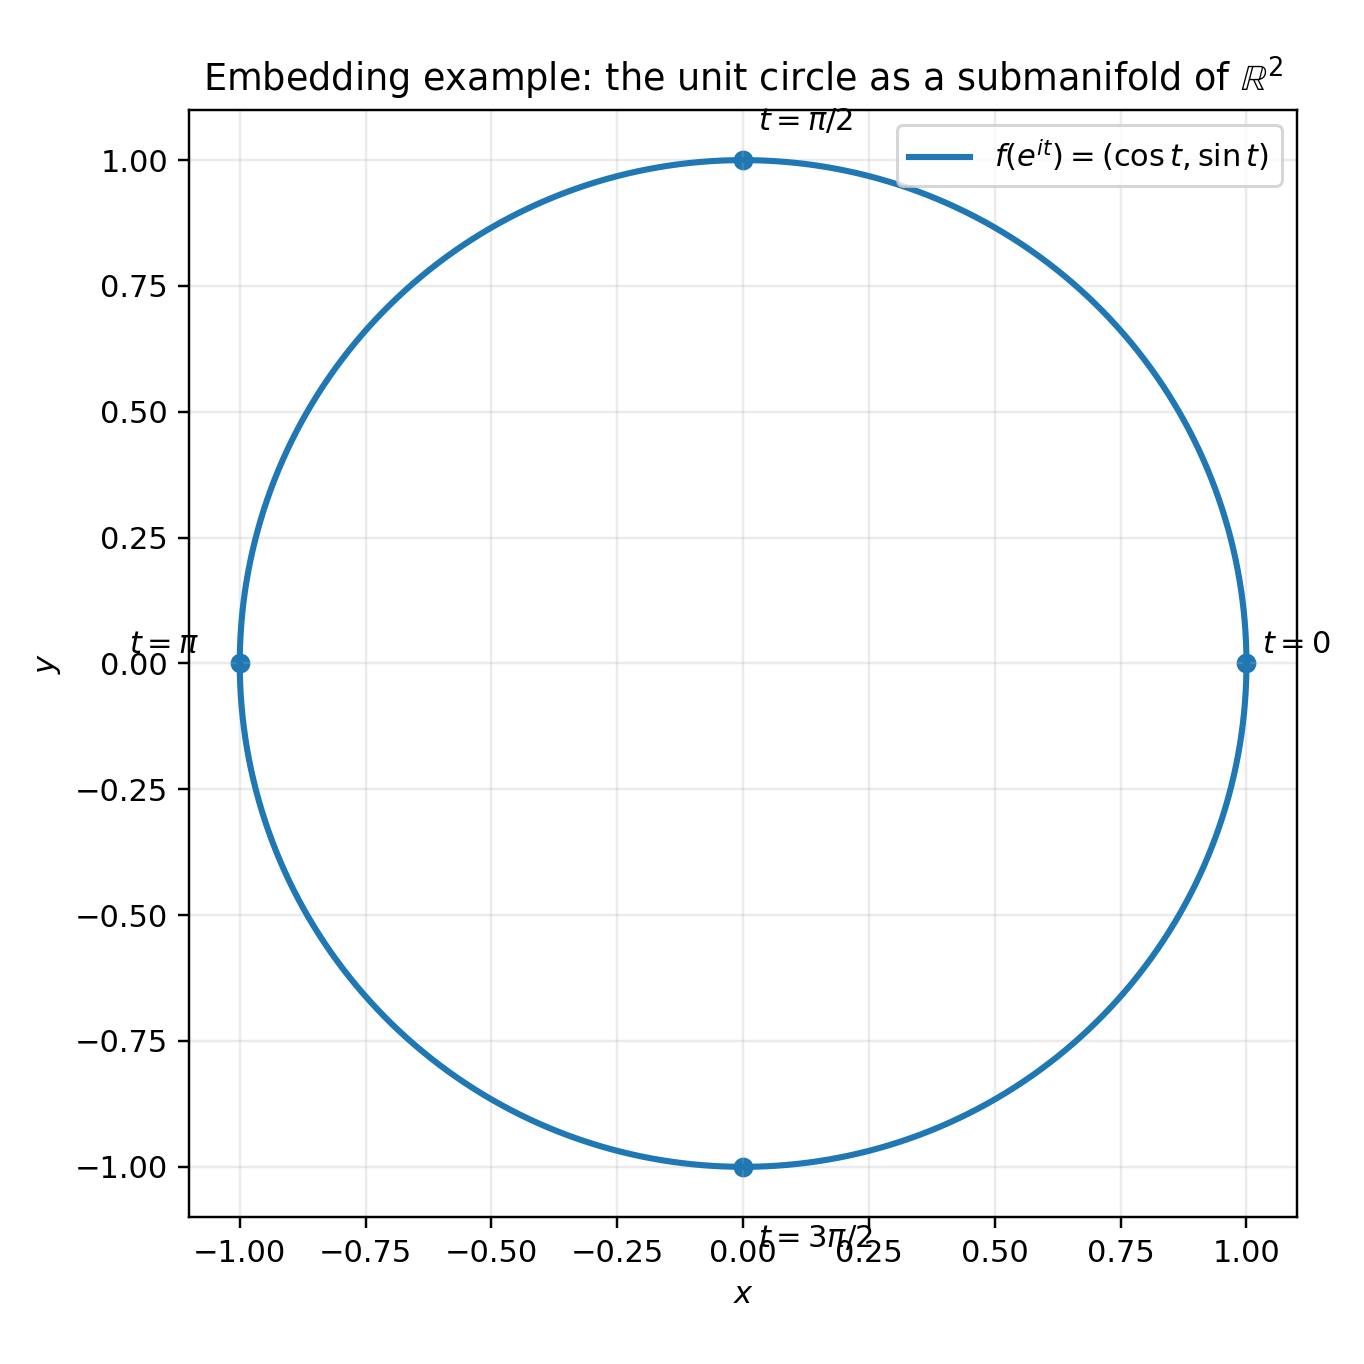
\includegraphics[width=0.58\textwidth]{chapters/part07_volume_vii/figures/problem6_embedding_circle.png}
	\caption{Embedding example: $S^1\hookrightarrow\mathbb{R}^2$, $f(e^{it})=(\cos t,\sin t)$.}
\end{figure}

\begin{figure}[htbp]
	\centering
	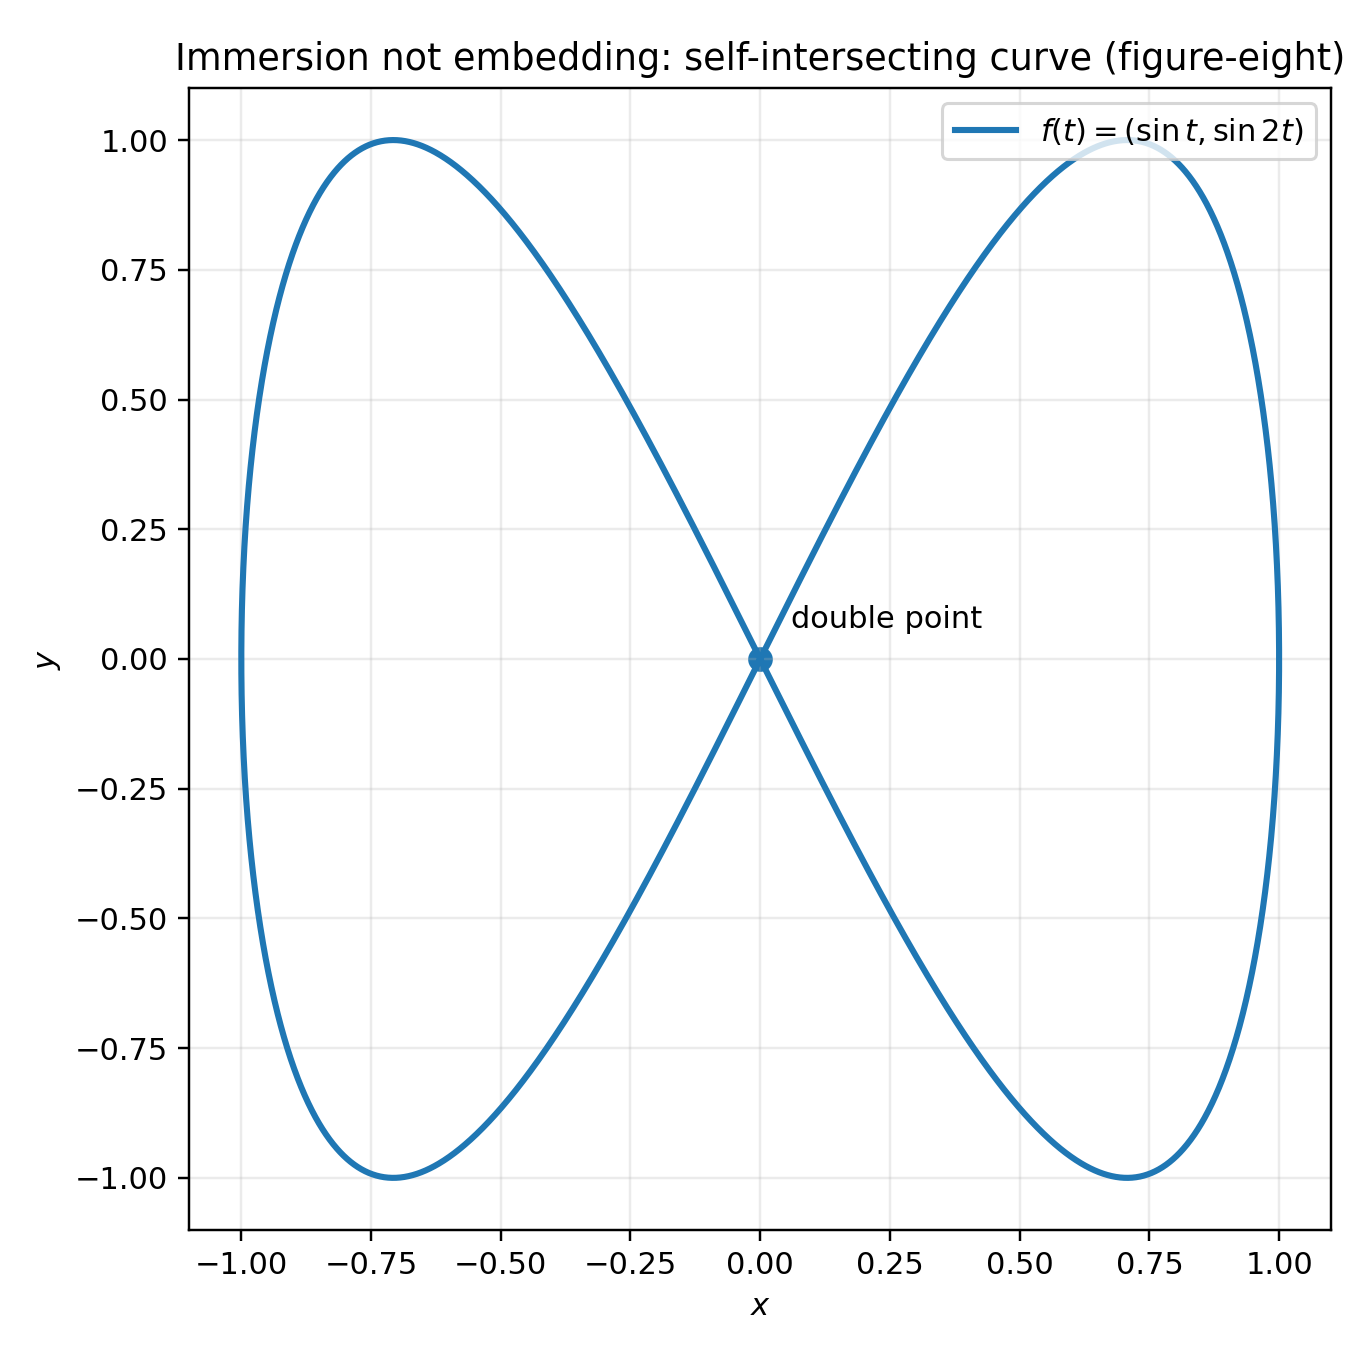
\includegraphics[width=0.58\textwidth]{chapters/part07_volume_vii/figures/problem6_immersion_figure_eight.png}
	\caption{Immersion not embedding: $f(t)=(\sin t,\sin 2t)$ has a self-intersection (double point).}
\end{figure}

\begin{figure}[htbp]
	\centering
	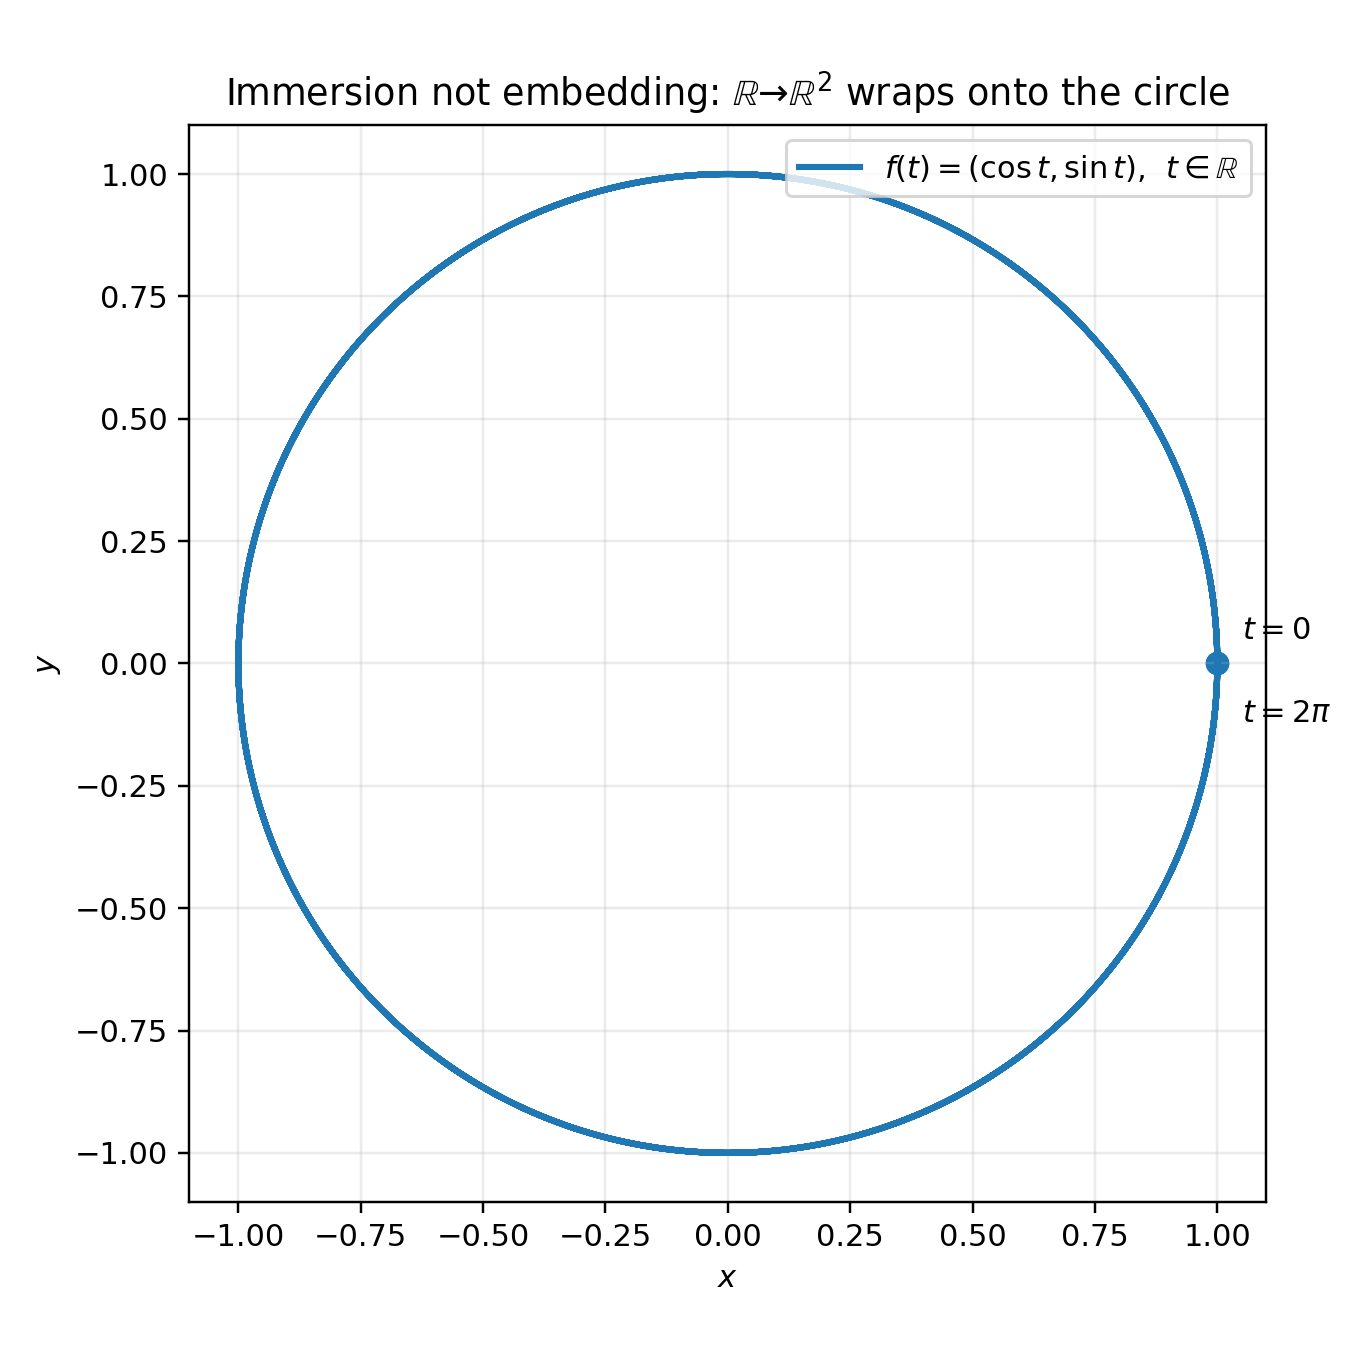
\includegraphics[width=0.58\textwidth]{chapters/part07_volume_vii/figures/problem6_immersion_R_wraps_circle.png}
	\caption{Immersion not embedding: $f:\mathbb{R}\to\mathbb{R}^2$, $f(t)=(\cos t,\sin t)$ is not injective.}
\end{figure}

% ------------------------------------------------------------
\end{solution}

\begin{problem}[CP-VII-0019 --- Problem 5 (Local normal form of a submersion)]
\label{prob:cp-vii-0019}
Let $X$ and $Y$ be manifolds of dimensions $n$ and $m$, and suppose $F:X\to Y$ is a submersion at $p$.
Construct an open neighbourhood $U$ of $p$ and a smooth map $G:U\to \mathbb{R}^{\,n-m}$ such that
$(F|_U,G):U\to Y\times \mathbb{R}^{\,n-m}$ is a local diffeomorphism at $p$.
Deduce that there exist local coordinates on $X$ and $Y$ about $p$ and $F(p)$ in which $F$ is given by
projection onto the first $m$ components.
\end{problem}

\begin{solution}
Choose charts $x=(x^1,\dots,x^n):U_0\to \mathbb{R}^n$ around $p$ and
$y=(y^1,\dots,y^m):V_0\to \mathbb{R}^m$ around $F(p)$, and set
$f:= y\circ F\circ x^{-1}:x(U_0)\subset\mathbb{R}^n\to \mathbb{R}^m$.
Since $F$ is a submersion at $p$, $\mathrm{rank}(Df)=m$ at $x(p)$, so some $m\times m$ minor is invertible.
After reordering $x^i$, assume
$\frac{\partial(f^1,\dots,f^m)}{\partial(x^1,\dots,x^m)}(x(p))$ is invertible.

Define $G=(x^{m+1},\dots,x^n)$ on a smaller neighbourhood $U\subset U_0$.
In coordinates let $g(x^1,\dots,x^n)=(x^{m+1},\dots,x^n)$ and $H=(f,g)$.
Then
\[
DH(x(p))=
\begin{pmatrix}
	\frac{\partial f}{\partial (x^1,\dots,x^m)} & \frac{\partial f}{\partial (x^{m+1},\dots,x^n)}\\
	0 & I_{n-m}
\end{pmatrix}
\]
is invertible, hence by the inverse function theorem $H$ is a local diffeomorphism at $x(p)$.
Therefore $(F|_U,G):U\to Y\times\mathbb{R}^{n-m}$ is a local diffeomorphism at $p$.

For the normal form, define coordinates on $X$ by
$\tilde x=(y^1\circ F,\dots,y^m\circ F,\,x^{m+1},\dots,x^n)$
and on $Y$ by $\tilde y=(y^1,\dots,y^m)$.
Then $\tilde y\circ F\circ \tilde x^{-1}(u^1,\dots,u^n)=(u^1,\dots,u^m)$, i.e.\ $F$ is projection.


\begin{figure}[h]
	\centering
	\[
	\begin{tikzcd}[row sep=large, column sep=large]
		U \subset X \arrow[r, "{(F,G)}"] \arrow[dr, "F"'] & Y \times \mathbb{R}^{n-m} \arrow[d, "\mathrm{pr}_1"] \\
		& Y
	\end{tikzcd}
	\]
	\caption{Problem 5: Local normal form of a submersion. The map $(F,G)$ is a local diffeomorphism and $F=\mathrm{pr}_1\circ (F,G)$.}
\end{figure}

\begin{figure}[h]
	\centering
	\renewcommand{\arraystretch}{1.35}
	\begin{tabular}{|c|c|c|}
		\hline
		\textbf{Object} & \textbf{Local coordinates} & \textbf{Form in coordinates} \\
		\hline
		Point in $X$ & $(u^1,\dots,u^m,\; u^{m+1},\dots,u^n)$ & --- \\
		\hline
		Point in $Y$ & $(u^1,\dots,u^m)$ & --- \\
		\hline
		Submersion $F$ & $(u^1,\dots,u^n)\mapsto (u^1,\dots,u^m)$ & $F=\mathrm{projection}$ \\
		\hline
		Complement $G$ & $(u^1,\dots,u^n)\mapsto (u^{m+1},\dots,u^n)$ & $G=\mathrm{remaining\ coords}$ \\
		\hline
		Combined map $(F,G)$ & $(u^1,\dots,u^n)\mapsto ((u^1,\dots,u^m),(u^{m+1},\dots,u^n))$ & local diffeo \\
		\hline
	\end{tabular}
	\caption{Problem 5: In adapted coordinates, $F$ becomes projection and $(F,G)$ becomes the identity to first order.}
\end{figure}
\end{solution}

\begin{problem}[CP-VII-0020 --- Problem 5]
\label{prob:cp-vii-0020}
\par\medskip\noindent\textbf{Problem.}\par\smallskip

Show that the set of all $2\times 2$ matrices of rank $1$ is a $3$-dimensional submanifold of $\mathbb{R}^4$.
\end{problem}

\begin{solution}
Identify $\mathbb{R}^4$ with matrices
\[
A=\begin{pmatrix}a&b\\ c&d\end{pmatrix}.
\]
Rank $1$ means $\det(A)=0$ but $A\neq 0$. Define the smooth function
\[
G:\mathbb{R}^4\to\mathbb{R},\qquad G(a,b,c,d)=ad-bc.
\]
Then
\[
\{A:\operatorname{rank}(A)=1\}=\{G=0\}\setminus\{0\}.
\]
Compute
\[
\nabla G(a,b,c,d)=(d,\,-c,\,-b,\,a).
\]
If $\nabla G=0$, then $a=b=c=d=0$, i.e.\ only at the zero matrix.
Therefore, on $\{G=0\}\setminus\{0\}$, the gradient is never zero, so $0$ is a regular value
(of $G$ restricted to $\mathbb{R}^4\setminus\{0\}$). Hence $\{G=0\}\setminus\{0\}$ is a smooth
embedded submanifold of codimension $1$ in $\mathbb{R}^4$, so it has dimension $4-1=3$.
\qed

% ------------------------------------------------------------
\end{solution}

\begin{problem}[CP-VII-0021 --- Problem 8 (Tangent space to a regular level set)]
\label{prob:cp-vii-0021}
Let $f:X\to Y$ be smooth and let $y\in Y$ be a regular value of $f$.
Show that for $x\in f^{-1}(y)$,
\[
T_x\bigl(f^{-1}(y)\bigr)=\ker\bigl(df_x:T_xX\to T_yY\bigr).
\]

\par\medskip\noindent\textbf{Theory / key fact.}\par\smallskip

If $y$ is a regular value, then for each $x\in f^{-1}(y)$ the differential $df_x$ is surjective, so $f$ is a submersion
along the level set. Locally, by the local submersion theorem, $f$ is a projection in suitable coordinates.
\end{problem}

\begin{solution}
\textbf{($\subset$)} Let $v\in T_x(f^{-1}(y))$. Then there exists a smooth curve
$\gamma:(-\varepsilon,\varepsilon)\to f^{-1}(y)$ with $\gamma(0)=x$ and $\gamma'(0)=v$.
Since $f(\gamma(t))=y$ is constant,
\[
0=\frac{d}{dt}\Big|_{t=0} f(\gamma(t))=df_x(\gamma'(0))=df_x(v),
\]
so $v\in\ker(df_x)$.

\medskip
\noindent\textbf{($\supset$)} Conversely, let $v\in\ker(df_x)$. Since $y$ is a regular value, $f$ is a submersion at $x$.
By the local submersion theorem, choose local coordinates $u=(u_1,\dots,u_k)$ near $x$ and coordinates near $y$ such that
\[
f(u_1,\dots,u_k)=(u_1,\dots,u_\ell),\qquad \ell=\dim Y.
\]
Then locally
\[
f^{-1}(y)=\{u_1=c_1,\dots,u_\ell=c_\ell\},
\]
so
\[
T_x(f^{-1}(y))=\operatorname{span}\Bigl\{\frac{\partial}{\partial u_{\ell+1}},\dots,\frac{\partial}{\partial u_k}\Bigr\}.
\]
In these coordinates $df_x$ is the projection onto the first $\ell$ components, hence
\[
\ker(df_x)=\operatorname{span}\Bigl\{\frac{\partial}{\partial u_{\ell+1}},\dots,\frac{\partial}{\partial u_k}\Bigr\}
= T_x(f^{-1}(y)).
\]
Therefore $T_x(f^{-1}(y))=\ker(df_x)$.
\qed

\begin{figure}[htbp]
	\centering
	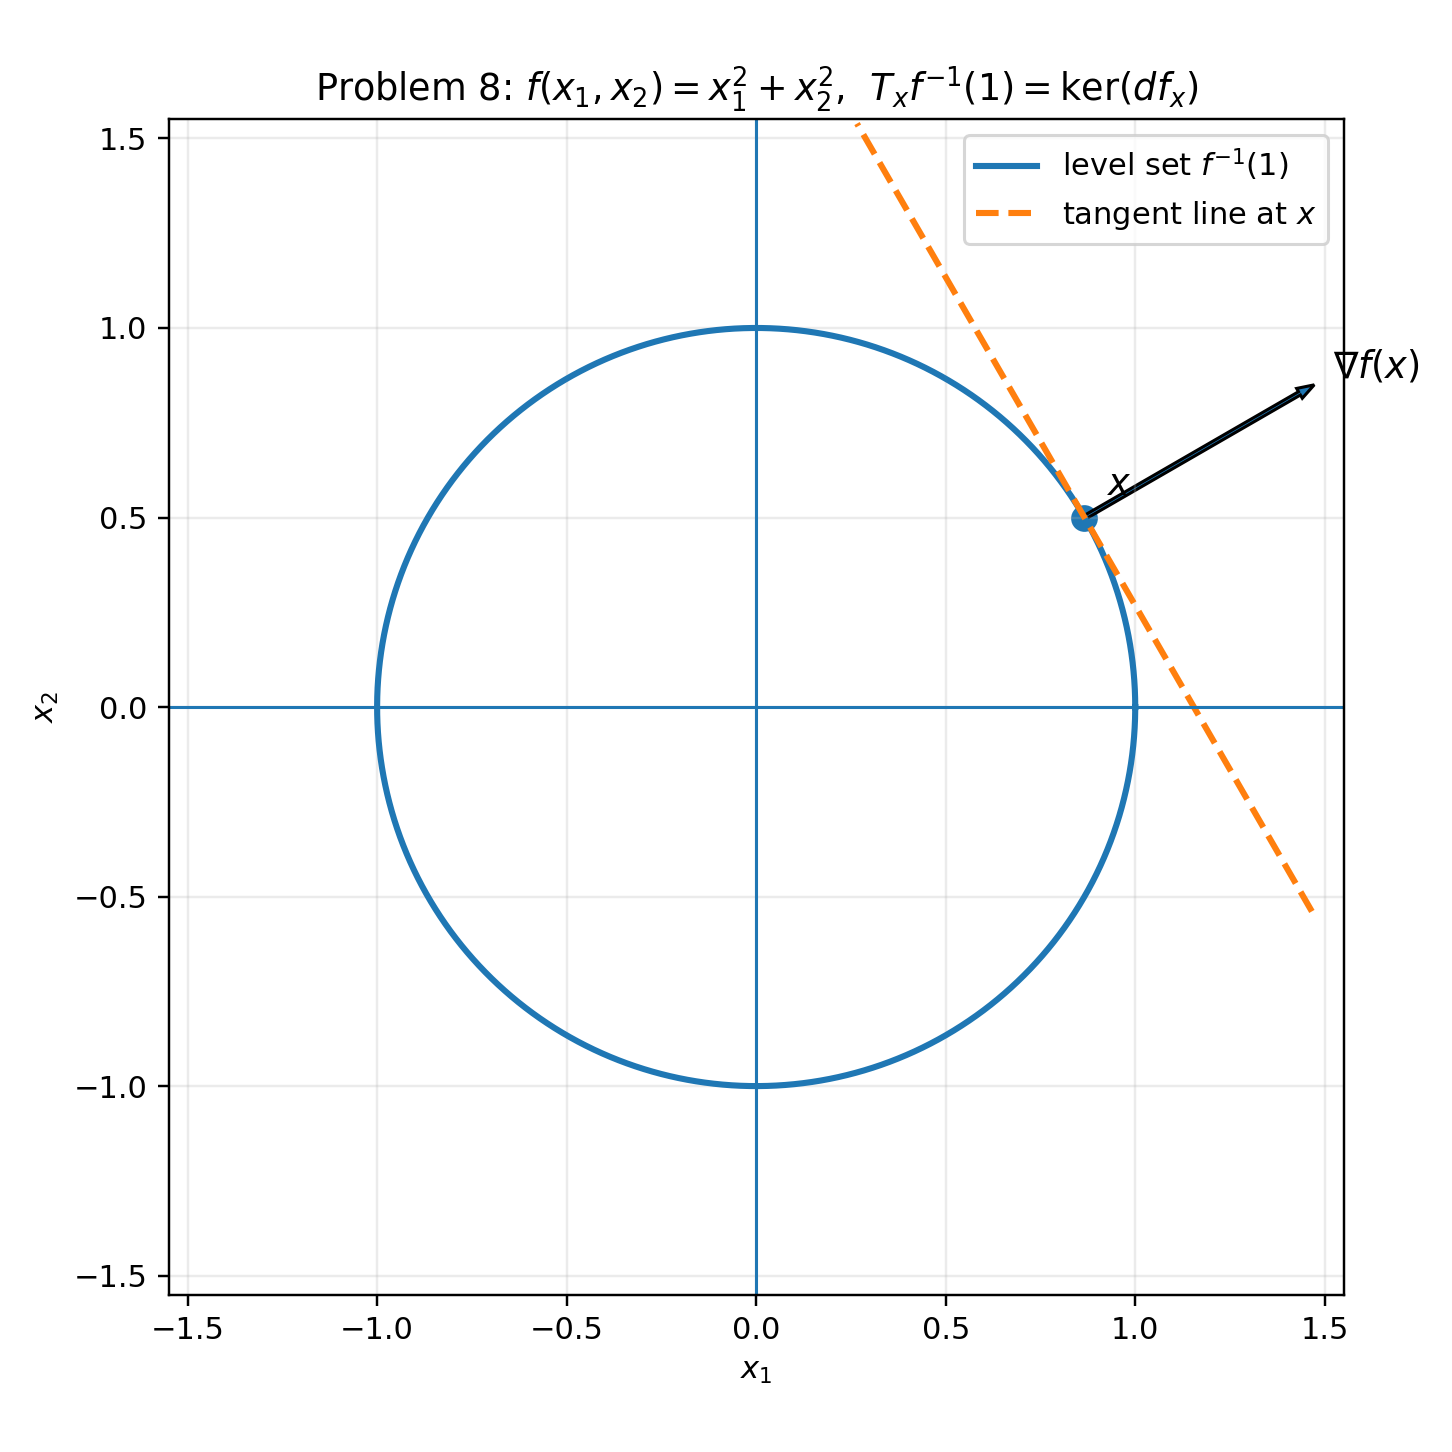
\includegraphics[width=0.62\textwidth]{chapters/part07_volume_vii/figures/problem8_circle_tangent_kernel.png}
	\caption{Problem 8: $f(x_1,x_2)=x_1^2+x_2^2$. The level set $f^{-1}(1)$ is a circle. 
		The tangent line at $x$ is orthogonal to $\nabla f(x)$, and equals $\ker(df_x)$.}
\end{figure}

\begin{figure}[htbp]
	\centering
	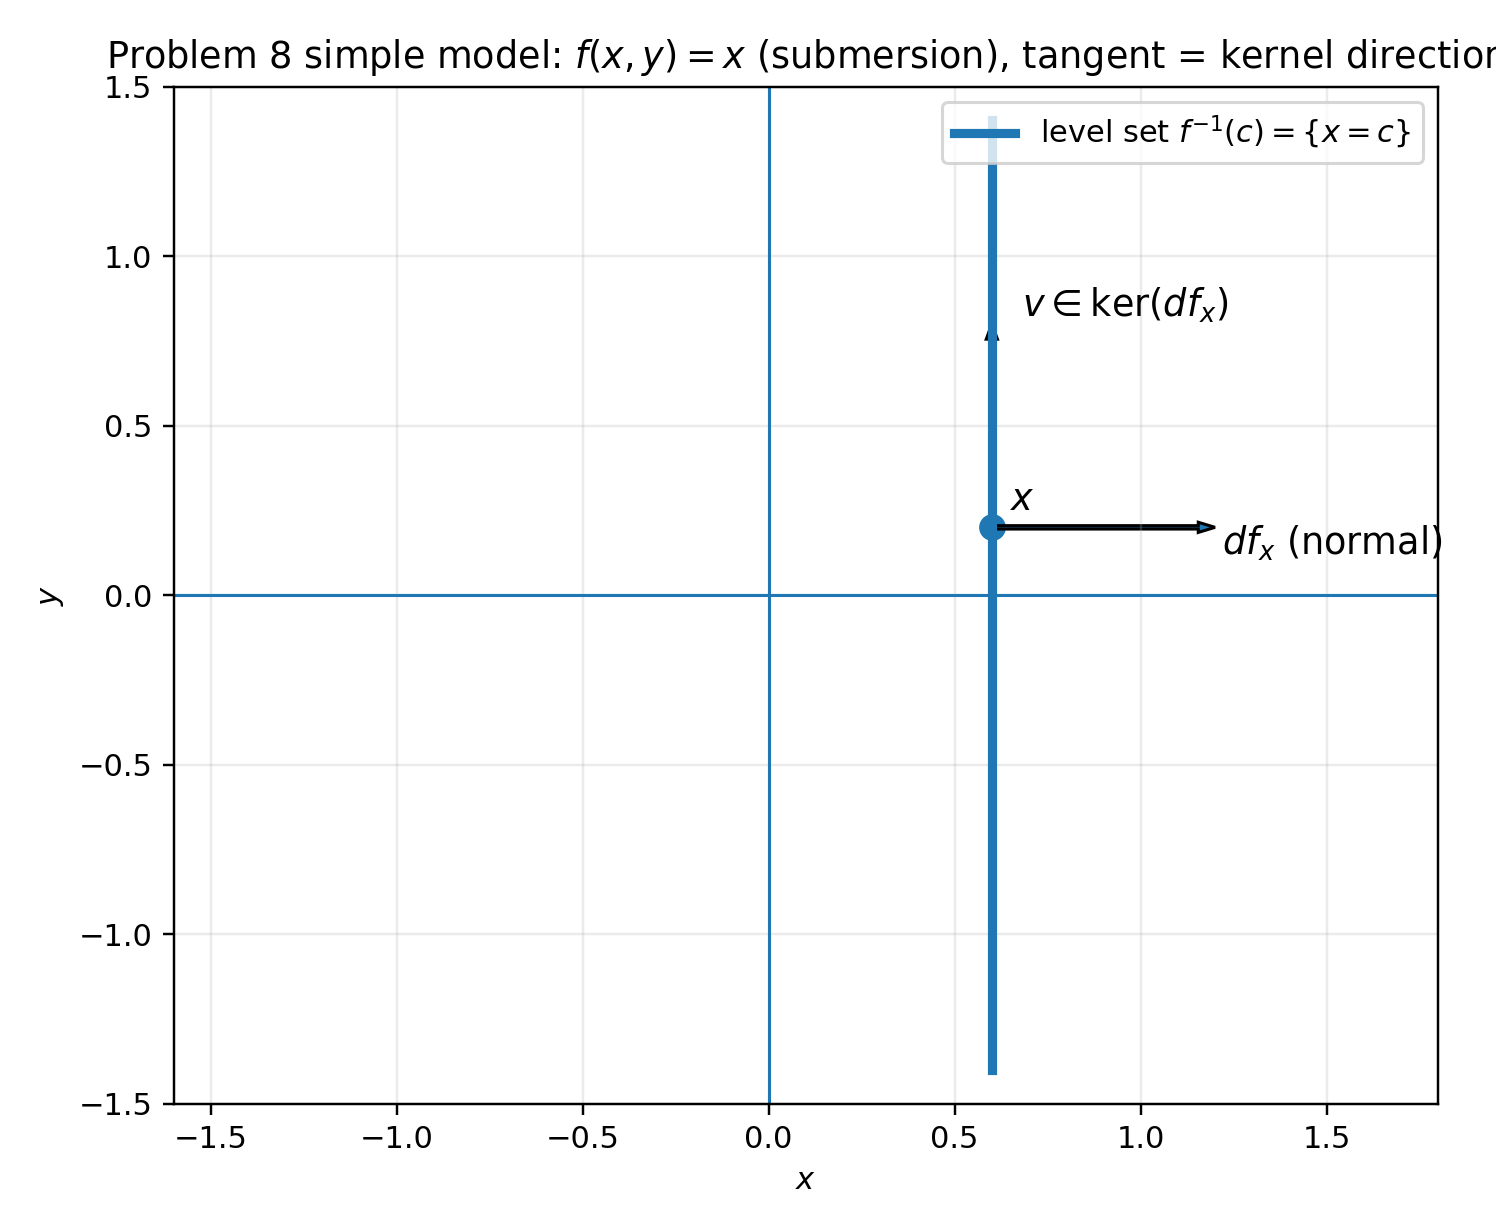
\includegraphics[width=0.78\textwidth]{chapters/part07_volume_vii/figures/problem8_projection_levelset_kernel.png}
	\caption{Problem 8 (model case): $f(x,y)=x$ is a submersion. The fiber $f^{-1}(c)=\{x=c\}$ has tangent direction $(0,1)$, which is exactly $\ker(df_x)$.}
\end{figure}

\begin{figure}[htbp]
	\centering
	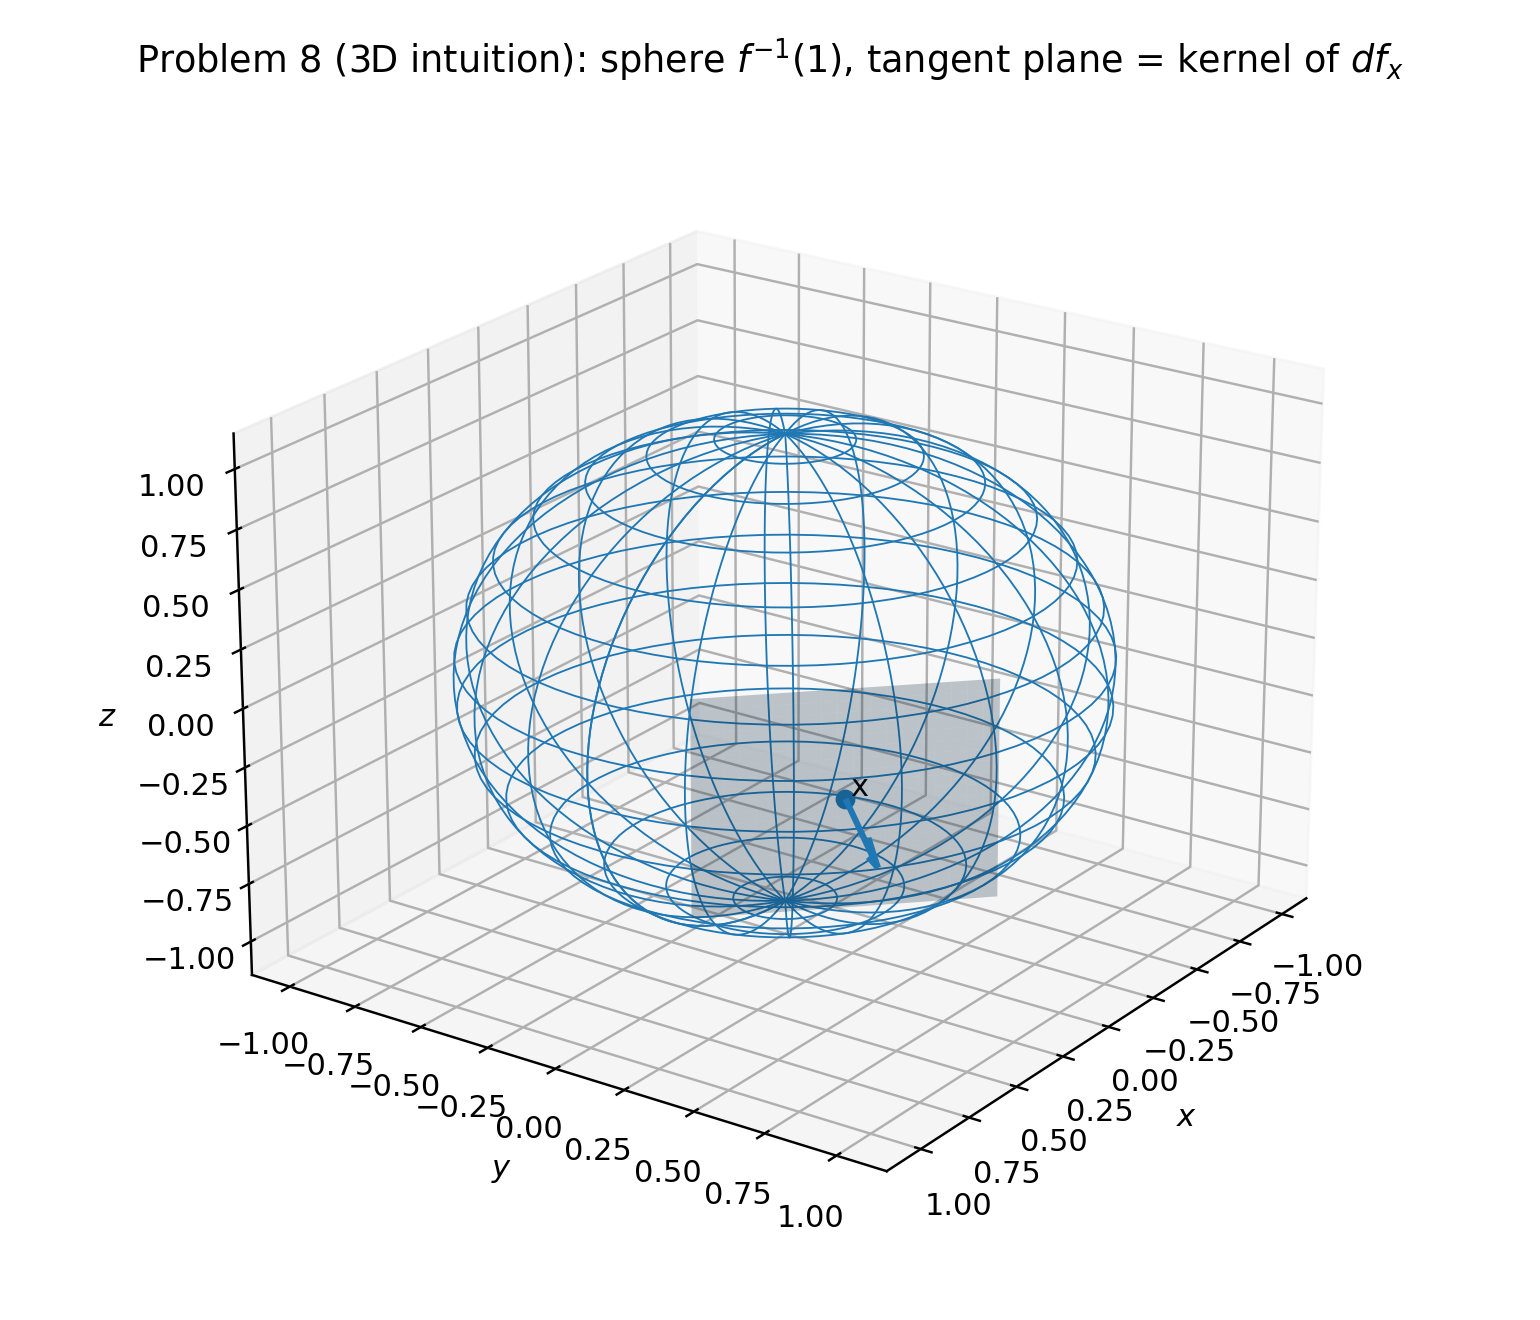
\includegraphics[width=0.70\textwidth]{chapters/part07_volume_vii/figures/problem8_sphere_tangent_plane.png}
	\caption{Problem 8 (3D intuition): for $f(x,y,z)=x^2+y^2+z^2$, the level set $f^{-1}(1)$ is the unit sphere. 
		The tangent plane at $x$ consists of vectors orthogonal to the normal direction (gradient), i.e.\ $\ker(df_x)$.}
\end{figure}

\begin{figure}[htbp]
	\centering
	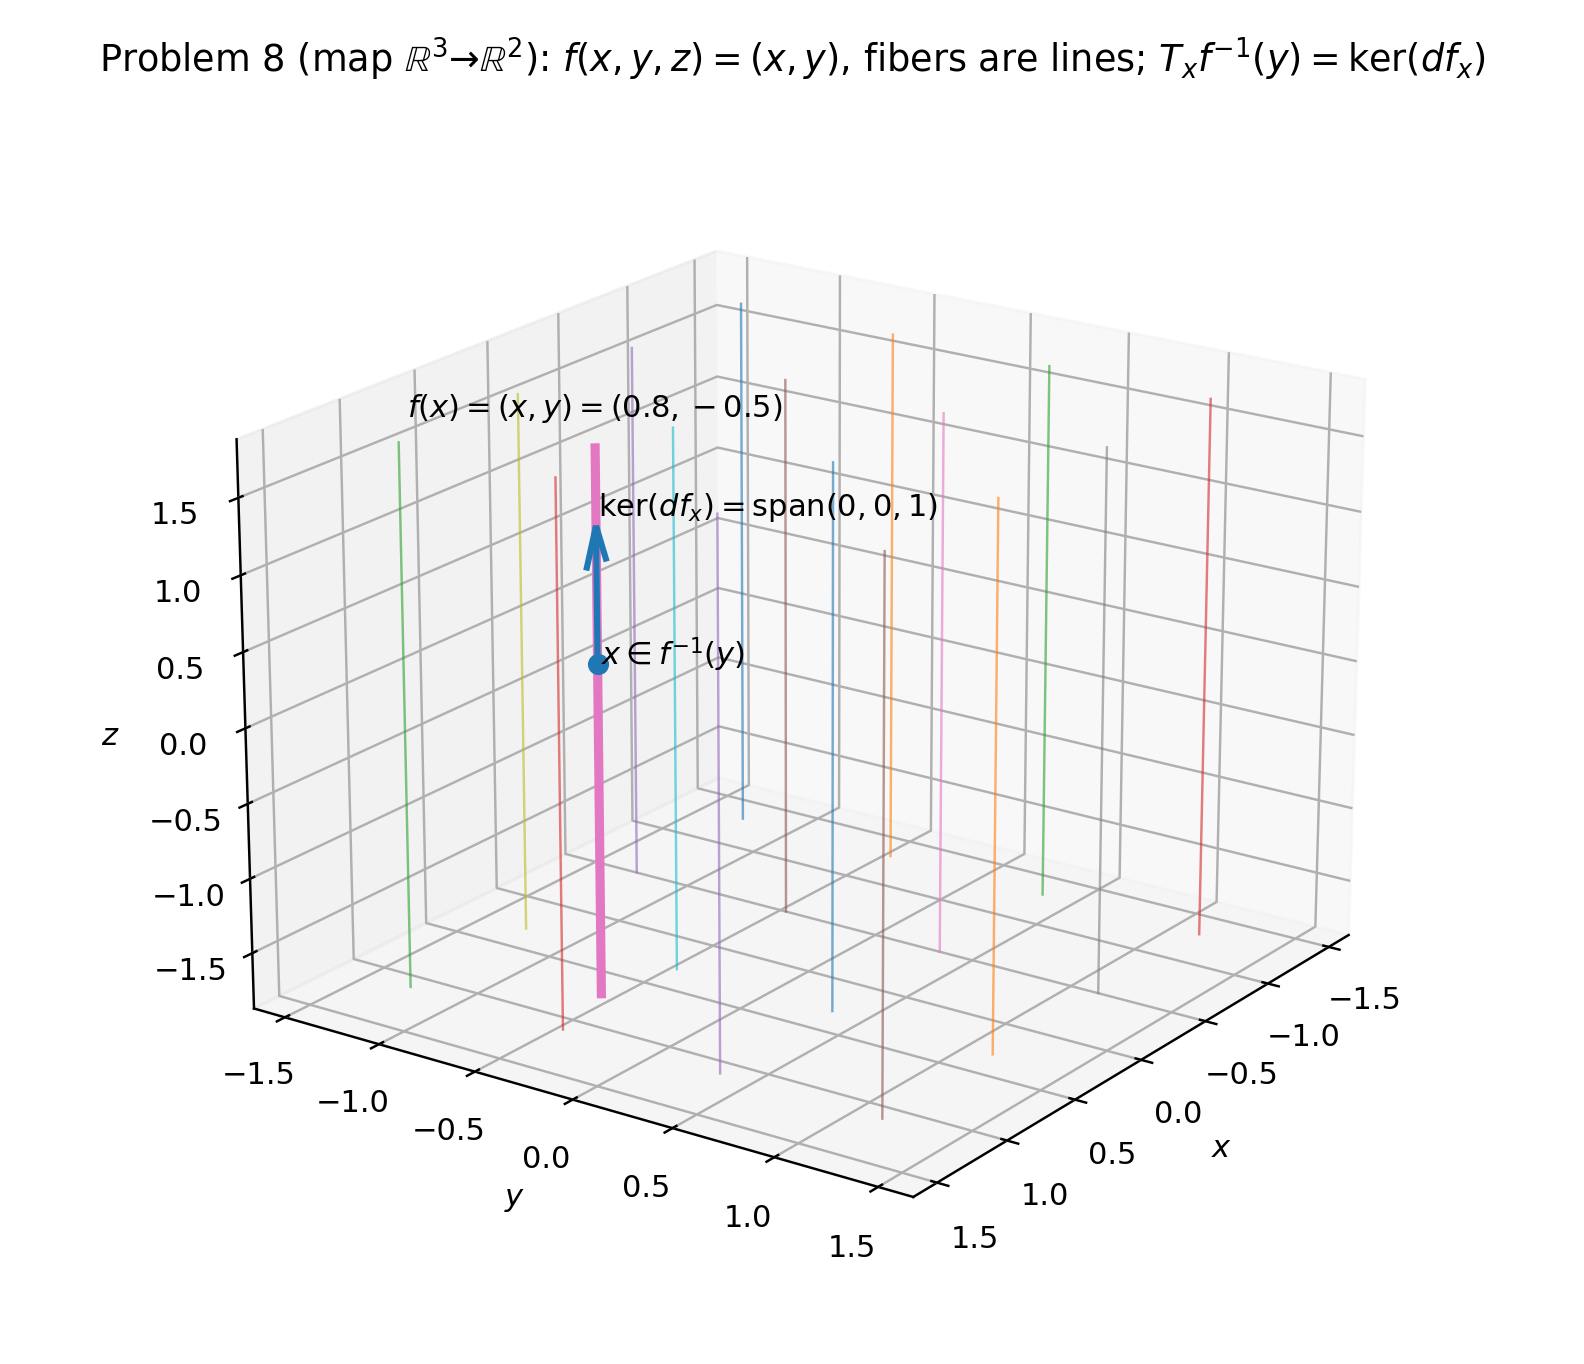
\includegraphics[width=0.70\textwidth]{chapters/part07_volume_vii/figures/problem8_R3_to_R2_projection_fiber_kernel.png}
	\caption{Problem 8 example: $f:\mathbb{R}^3\to\mathbb{R}^2$, $f(x,y,z)=(x,y)$. 
		For $y_0=(a,b)$, the fiber $f^{-1}(y_0)=\{(a,b,z)\}$ is a line. Its tangent direction is the $z$-direction,
		which equals $\ker(df_x)$ since $df_x(v_x,v_y,v_z)=(v_x,v_y)$.}
\end{figure}

\clearpage
\end{solution}

\begin{problem}[CP-VII-0022 --- Orthogonal and special unitary groups]
\label{prob:cp-vii-0022}
\begin{enumerate}
\item[(a)] Let \(\mathrm{Sym}(n)\) denote the symmetric \(n\times n\) matrices and consider
\[
F:GL(n,\mathbb R)\longrightarrow \mathrm{Sym}(n),
\qquad
F(A)=A^TA.
\]
Show that \(O(n)\) is an embedded Lie subgroup of \(GL(n,\mathbb R)\), and identify
\(\mathfrak o(n)\subset\mathfrak{gl}(n,\mathbb R)\).

\item[(b)] Show that \(SU(n)\) is a Lie subgroup of \(GL(n,\mathbb C)\), and identify its Lie algebra.
\end{enumerate}
\end{problem}

\begin{solution}
(a) Let $\mathrm{Sym}(n)=\{S\in M_n(\mathbb R):S^T=S\}$ and define $F(A)=A^TA$.
Then
\[
O(n)=\{A\in GL(n,\mathbb R):A^TA=I\}=F^{-1}(I).
\]
Identify $T_AGL(n,\mathbb R)\cong M_n(\mathbb R)$. For $B\in M_n(\mathbb R)$,
\[
(dF)_A(B)=\frac{d}{dt}\Big|_{0}(A+tB)^T(A+tB)=B^TA+A^TB\in\mathrm{Sym}(n).
\]
If $A\in O(n)$ and $S\in\mathrm{Sym}(n)$ is arbitrary, choose $B=\tfrac12 AS$. Then
\[
(dF)_A(B)=\tfrac12 S^T(A^TA)+\tfrac12(A^TA)S=\tfrac12 S^T+\tfrac12 S=S,
\]
so $(dF)_A$ is surjective. Hence $I$ is a regular value of $F$ and $O(n)=F^{-1}(I)$
is an embedded submanifold of $GL(n,\mathbb R)$. Since it is a subgroup, it is an embedded Lie subgroup.

Its Lie algebra is $T_IO(n)$. Differentiating $A^TA=I$ at $A=I$ gives
\[
0=\frac{d}{dt}\Big|_{0}(A(t)^TA(t))=X^T+X,
\]
so
\[
\mathfrak o(n)=\{X\in\mathfrak{gl}(n,\mathbb R):X^T+X=0\},
\]
the skew-symmetric matrices.

(b) Let $U(n)=\{A\in GL(n,\mathbb C):A^*A=I\}$ and $SU(n)=\{A\in U(n):\det A=1\}$.
As in (a), the map $F_{\mathbb C}(A)=A^*A$ has $U(n)=F_{\mathbb C}^{-1}(I)$, hence $U(n)$ is an embedded Lie subgroup.

The determinant $\det:U(n)\to S^1$ is smooth and $SU(n)=\det^{-1}(1)$.
Its differential at $I$ satisfies
\[
\frac{d}{dt}\Big|_{0}\det(I+tX)=\mathrm{tr}(X).
\]
For $X\in\mathfrak u(n)=T_IU(n)=\{X:X^*+X=0\}$, $\mathrm{tr}(X)\in i\mathbb R\cong T_1S^1$,
and the map $X\mapsto \mathrm{tr}(X)$ is surjective (e.g.\ $X=i\lambda I$).
Thus $1$ is a regular value and $SU(n)$ is an embedded Lie subgroup of $U(n)\subset GL(n,\mathbb C)$.

Finally,
\[
\mathfrak{su}(n)=\{X\in\mathfrak{gl}(n,\mathbb C):X^*+X=0,\ \mathrm{tr}(X)=0\}.
\]

\par\medskip\noindent\textbf{Theory for Problem 8 (matrix Lie groups and Lie algebras)}\par\smallskip


\textbf{Matrix Lie groups.}
A matrix Lie group is a subgroup $G\subset GL(N,\mathbb F)$ that is an embedded submanifold.

\textbf{Lie algebra.}
The Lie algebra is $\mathfrak g=T_I G\subset M_N(\mathbb F)$, with bracket $[X,Y]=XY-YX$.
Equivalently,
\[
\mathfrak g = \{X\in M_N(\mathbb F): \exp(tX)\in G \text{ for all small } t\}.
\]

\textbf{Regular level sets.}
If $F:GL(N,\mathbb F)\to W$ is smooth and $c$ is a regular value, then $F^{-1}(c)$ is an embedded submanifold.

\textbf{Standard examples.}
\[
O(n)=\{A\in GL(n,\mathbb R):A^TA=I\},\quad
\mathfrak o(n)=\{X:X^T+X=0\}.
\]
\[
U(n)=\{A\in GL(n,\mathbb C):A^*A=I\},\quad
\mathfrak u(n)=\{X:X^*+X=0\}.
\]
\[
SU(n)=\{A\in U(n):\det A=1\},\quad
\mathfrak{su}(n)=\{X\in\mathfrak u(n):\mathrm{tr}\,X=0\}.
\]

\begin{figure}[h]
	\centering
	\renewcommand{\arraystretch}{1.35}
	\begin{tabular}{|c|c|c|}
		\hline
		\textbf{Group} & \textbf{Defining constraint} & \textbf{Lie algebra condition at $I$} \\
		\hline
		$O(n)$ & $A^TA=I$ & $X^T+X=0$ (skew-symmetric) \\
		\hline
		$U(n)$ & $A^*A=I$ & $X^*+X=0$ (skew-Hermitian) \\
		\hline
		$SU(n)$ & $A^*A=I$, $\det A=1$ & $X^*+X=0$, $\mathrm{tr}(X)=0$ \\
		\hline
	\end{tabular}
	\caption{Problem 8: Matrix Lie groups as constraint sets and their Lie algebras from differentiation at the identity.}
\end{figure}

\begin{figure}[h]
	\centering
	\renewcommand{\arraystretch}{1.35}
	\begin{tabular}{|p{0.28\linewidth}|p{0.68\linewidth}|}
		\hline
		\textbf{Step} & \textbf{What to write} \\
		\hline
		Define $F$ & $F:GL(n,\mathbb{R})\to \mathrm{Sym}(n),\quad F(A)=A^TA$ \\
		\hline
		Level set & $O(n)=F^{-1}(I)$ \\
		\hline
		Differentiate & $(dF)_I(X)=X^T+X$ \\
		\hline
		Kernel & $T_IO(n)=\ker(dF)_I=\{X:X^T+X=0\}=\mathfrak{o}(n)$ \\
		\hline
		Analog for $SU(n)$ & Use $F(A)=A^*A$ plus $\det(A)=1$; get $X^*+X=0$ and $\mathrm{tr}(X)=0$ \\
		\hline
	\end{tabular}
	\caption{Problem 8: Proof skeleton chart (regular level set + tangent space computation).}
\end{figure}

\begin{figure}[h]
	\centering
	\renewcommand{\arraystretch}{1.35}
	\begin{tabular}{|c|p{0.36\linewidth}|p{0.54\linewidth}|}
		\hline
		\textbf{Prob.} & \textbf{Main tool} & \textbf{Main takeaway} \\
		\hline
		5 & Inverse Function Theorem & Submersion $\Rightarrow$ local product coordinates, $F$ becomes projection \\
		\hline
		6 & Sard's Theorem & If $\dim X<\dim Y$, image has measure $0$ $\Rightarrow$ no surjective smooth map \\
		\hline
		7 & ODE + Frobenius idea & Horizontal lifts exist/unique; integrability $\Leftrightarrow$ endpoint-only transport \\
		\hline
		8 & Regular level set + tangent space & $O(n),SU(n)$ are embedded Lie subgroups; compute Lie algebras by differentiating constraints \\
		\hline
	\end{tabular}
	\caption{Problems 5--8: Tools and conclusions.}
\end{figure}
\end{solution}

\begin{problem}[CP-VII-0023 --- Problem 4]
\label{prob:cp-vii-0023}
\begin{enumerate}[label=\textnormal{(\alph*)}]
	
	% ------------------------------------------------------------
	% (a)
	% ------------------------------------------------------------
	\item 
	Consider a decomposition of a topological surface into polygons
	(with $V$ vertices, $E$ edges and $F$ faces), where all vertices
	have valence $\ge 3$ and every face contains $\ge 3$ vertices.
	Let $F_{n}$ denote the number of faces bounded by precisely $n$ edges,
	and $V_{m}$ the number of vertices where precisely $m$ edges meet.
	Show that
	\[
	\sum_{n} n F_{n} = 2E = \sum_{m} m V_{m}.
	\]
	If $V_{3} = 0$, deduce $E \ge 2V$.
	If $F_{3} = 0$, deduce $E \ge 2F$.
	If the surface is a sphere, deduce that $V_{3} + F_{3} > 0$.
	
	\medskip

\end{enumerate}\end{problem}

\begin{solution}
Each edge is contained in exactly two faces.  
	Counting incidences (face, edge on that face) in two ways yields
	\[
	\sum_n nF_n = 2E.
	\]
	Similarly, each edge has two endpoints.  Counting incidences
	(vertex, edge incident at that vertex) gives
	\[
	\sum_m mV_m = 2E.
	\]
	Hence
	\[
	\sum_n nF_n = 2E = \sum_m mV_m.
	\]
	
	If $V_3 = 0$ and each vertex has valence at least $3$, then every vertex
	has valence at least $4$, so
	\[
	2E = \sum_m mV_m \ge 4V,
	\]
	and therefore $E \ge 2V$.
	
	If $F_3 = 0$ and each face has at least $3$ edges, then each face has at least
	$4$ edges, so
	\[
	2E = \sum_n nF_n \ge 4F,
	\]
	hence $E \ge 2F$.
	
	If the surface is the sphere, Euler's formula
	\[
	V - E + F = 2
	\]
	holds. If $V_3 = F_3 = 0$, then $E \ge 2V$ and $E \ge 2F$, so
	$V \le E/2$ and $F \le E/2$. Thus
	\[
	V - E + F \le \frac{E}{2} - E + \frac{E}{2} = 0,
	\]
	contradicting $V - E + F = 2$.  
	Hence $V_3 + F_3 > 0$.
	
	% ------------------------------------------------------------
	% (b)
	% ------------------------------------------------------------
	\par\smallskip\noindent\textbullet\enspace 
	For a polygonal decomposition of a sphere, show that
	\[
	\sum_{n} (6-n) F_{n}
	= 12 + 2 \sum_{m} (m-3) V_{m}.
	\]
	If each face has at least $3$ edges and at least $3$ edges meet
	at each vertex, deduce that
	\[
	3F_{3} + 2F_{4} + F_{5} \ge 12.
	\]
	
	\medskip
	\textbf{Solution.}
	We compute
	\[
	\sum_n (6-n)F_n
	= 6\sum_n F_n - \sum_n nF_n
	= 6F - 2E,
	\]
	since $\sum_n F_n = F$ and $\sum_n nF_n = 2E$.
	
	Similarly,
	\[
	\sum_m (m-3)V_m
	= \sum_m mV_m - 3\sum_m V_m
	= 2E - 3V,
	\]
	because $\sum_m mV_m = 2E$ and $\sum_m V_m = V$.
	
	Hence
	\[
	12 + 2\sum_m (m-3)V_m
	= 12 + 2(2E - 3V)
	= 12 + 4E - 6V.
	\]
	
	Using Euler's formula $V - E + F = 2$ on the sphere, we have
	$F = 2 - V + E$. Thus
	\[
	6F - 2E
	= 6(2 - V + E) - 2E
	= 12 - 6V + 4E.
	\]
	Thus
	\[
	\sum_n (6-n)F_n = 12 + 2\sum_m (m-3)V_m.
	\]
	
	If each face has at least 3 edges and each vertex has valence at least 3,
	then $(m-3)V_m \ge 0$ for all $m$, so
	\[
	\sum_n (6-n)F_n \ge 12.
	\]
	Now
	\[
	\sum_n (6-n)F_n
	= 3F_3 + 2F_4 + F_5 + 0\cdot F_6 
	+ \sum_{n\ge 7} (6-n)F_n.
	\]
	For $n \ge 6$, the terms $(6-n)$ are nonpositive, so
	\[
	3F_3 + 2F_4 + F_5 \ge 12.
	\]
	
	% ------------------------------------------------------------
	% (c)
	% ------------------------------------------------------------
	\par\smallskip\noindent\textbullet\enspace 
	The surface of a football is decomposed into hexagons and pentagons,
	with precisely $3$ faces meeting at each vertex.
	How many pentagons are there?
	
	\medskip
	\textbf{Solution.}
	Faces are only pentagons and hexagons, so $F_n=0$ unless $n=5,6$.
	Each vertex has valence $3$, so $V_3 = V$ and $V_m = 0$ for $m \ne 3$.
	
	Using the identity proved in (b),
	\[
	\sum_n (6-n)F_n = 12 + 2\sum_m (m-3)V_m.
	\]
	Since $m-3=0$ for $m=3$, the right-hand side is simply $12$.
	
	The left-hand side is
	\[
	(6-5)F_5 + (6-6)F_6 = F_5.
	\]
	Hence $F_5 = 12$.

\end{solution}

\begin{problem}[CP-VII-0024 --- Problem 6 --- Intersection of Two Surfaces Gives a Smooth Curve]
\label{prob:cp-vii-0024}
A \emph{smooth curve} in $\mathbb{R}^3$ is a subspace which can locally be
	given as the image of a smooth injective map
	\[
	(-1,1) \to \mathbb{R}^3
	\]
	with injective differential.
	
	Let
	\[
	H : \mathbb{R}^3 \to \mathbb{R},
	\qquad
	K : \mathbb{R}^3 \to \mathbb{R}
	\]
	be smooth functions.
	Suppose the level sets
	\[
	H^{-1}(0)
	\qquad\text{and}\qquad
	K^{-1}(0)
	\]
	are smooth surfaces in $\mathbb{R}^3$ which intersect along a smooth curve
	$\gamma$.
	
	Let $p = (x_0,y_0,z_0) \in \gamma$, and assume that at $p$ the expression
	\[
	K_y H_z \;-\; K_z H_y
	\]
	is non-vanishing.
	
	Show that, in some neighbourhood of $p$, the curve $\gamma$ can be parametrized
	by the variable $x$.  If we write
	\[
	\gamma(x) = (x, y(x), z(x)),
	\]
	then prove that
	\[
	y'(x)
	= \frac{K_z H_x - K_x H_z}{K_y H_z - K_z H_y}.
	\]
	
	\bigskip
	
	
	\par\medskip\noindent\textbf{Smooth Curves: Definition and Charts}\par\smallskip

	
	A subset $\gamma \subset \mathbb{R}^3$ is called a \emph{smooth curve} if
	every point $p\in\gamma$ has a neighbourhood $U\subset\gamma$ for which there
	exists a smooth injective map
	\[
	\alpha : (-1,1) \longrightarrow \mathbb{R}^3
	\]
	with non-vanishing derivative $\alpha'(t)\neq 0$ such that
	$\alpha((-1,1)) = U$.
	Thus a smooth curve is a $1$--dimensional embedded smooth submanifold of
	$\mathbb{R}^3$.
	
	\par\medskip\noindent\textbf{Regular parametrizations}\par\smallskip

	A smooth map $\alpha : I \to \mathbb{R}^3$ is a \emph{regular
		parametrization} if $\alpha'(t)\neq 0$ for all $t\in I$.
	If $\alpha$ is regular, then $\gamma=\alpha(I)$ is a smooth curve, and
	conversely every smooth curve is locally the image of a regular parametrization.
	
	\par\medskip\noindent\textbf{Charts on a smooth curve}\par\smallskip

	Let $\gamma$ be a smooth curve and let
	$\alpha : I \to \gamma$ be a regular parametrization.
	Then
	\[
	\varphi = \alpha^{-1} : U=\alpha(I) \to I
	\]
	defines a smooth chart on $U$.
	Transition maps between such charts are smooth because changes of
	parametrization are smooth.
	Hence every smooth curve carries a natural structure of a $1$--dimensional
	smooth manifold.
	
	\par\medskip\noindent\textbf{Geometric sources of smooth curves}\par\smallskip

	\begin{itemize}
		\item Intersections of smooth surfaces $H^{-1}(0)\cap K^{-1}(0)$,
		provided the gradients are transverse.
		\item Level sets $f^{-1}(c)$ in $\mathbb{R}^2$ with $\nabla f \neq 0$.
		\item Images of regular embeddings $\alpha : \mathbb{R}\to\mathbb{R}^3$.
	\end{itemize}
	
	 \emph{smooth curve} in $\mathbb{R}^3$ is a subspace which can locally be
	given as the image of a smooth injective map
	\[
	(-1,1) \to \mathbb{R}^3
	\]
	with injective differential.
	
	Let
	\[
	H : \mathbb{R}^3 \to \mathbb{R}, \qquad
	K : \mathbb{R}^3 \to \mathbb{R}
	\]
	be smooth functions.
	Suppose the level sets
	\[
	H^{-1}(0) \quad\text{and}\quad K^{-1}(0)
	\]
	are smooth surfaces in $\mathbb{R}^3$ which intersect along a smooth curve
	$\gamma$.
	Suppose $p = (x_0,y_0,z_0)$ belongs to $\gamma$, and that at $p$ the expression
	$K_y H_z - K_z H_y$ is non-vanishing.
	
	\begin{enumerate}[label=\textnormal{(\alph*)}]
		\item Show that in some neighbourhood of $p$ the curve $\gamma$ can be
		parametrized by the variable $x$, and that if we write
		\[
		\gamma(x) = (x,y(x),z(x)),
		\]
		then
		\[
		y'(x) = \frac{K_z H_x - K_x H_z}{K_y H_z - K_z H_y}.
		\]
	\end{enumerate}
	
	\medskip
\end{problem}

\begin{solution}
Define
	\[
	F : \mathbb{R}^3 \to \mathbb{R}^2, \qquad
	F(x,y,z) = \bigl(H(x,y,z),\,K(x,y,z)\bigr).
	\]
	Then $\gamma$ is exactly the zero set of $F$,
	\[
	\gamma = F^{-1}(0,0),
	\]
	and at the point $p=(x_0,y_0,z_0)$ we have
	\[
	K_y H_z - K_z H_y \neq 0.
	\]
	Consider the Jacobian of $F$ with respect to the variables $(y,z)$:
	\[
	D_{(y,z)}F(x,y,z)
	=
	\begin{pmatrix}
		H_y & H_z \\
		K_y & K_z
	\end{pmatrix}.
	\]
	Its determinant is
	\[
	\det D_{(y,z)}F
	= H_y K_z - H_z K_y
	= -(K_y H_z - K_z H_y),
	\]
	which is non-zero at $p$ by assumption.  Therefore, by the implicit function
	theorem, there exist an open interval $I$ containing $x_0$ and smooth
	functions $y,z : I \to \mathbb{R}$ such that
	\[
	F\bigl(x,y(x),z(x)\bigr) = (0,0)
	\]
	for all $x\in I$.  In particular, near $p$ the intersection curve $\gamma$ is
	parametrized by
	\[
	\gamma(x) = \bigl(x,y(x),z(x)\bigr),
	\]
	so $x$ is a valid parameter.
	
	Since for all $x\in I$ we have
	\[
	H\bigl(x,y(x),z(x)\bigr) = 0,
	\qquad
	K\bigl(x,y(x),z(x)\bigr) = 0,
	\]
	differentiating with respect to $x$ yields
	\begin{align*}
		H_x + H_y\,y'(x) + H_z\,z'(x) &= 0, \\
		K_x + K_y\,y'(x) + K_z\,z'(x) &= 0.
	\end{align*}
	This is a linear system for the unknowns $y'(x)$ and $z'(x)$:
	\[
	\begin{cases}
		H_y\,y' + H_z\,z' = -H_x,\\
		K_y\,y' + K_z\,z' = -K_x.
	\end{cases}
	\]
	Let
	\[
	\Delta = \det
	\begin{pmatrix}
		H_y & H_z \\
		K_y & K_z
	\end{pmatrix}
	= H_y K_z - H_z K_y
	= -(K_y H_z - K_z H_y) \neq 0.
	\]
	By Cramer's rule, the numerator for $y'$ is
	\[
	\det
	\begin{pmatrix}
		-H_x & H_z \\
		-K_x & K_z
	\end{pmatrix}
	= (-H_x)K_z - H_z(-K_x)
	= H_z K_x - H_x K_z.
	\]
	Thus
	\[
	y'
	= \frac{H_z K_x - H_x K_z}{H_y K_z - H_z K_y}
	= \frac{K_z H_x - K_x H_z}{K_y H_z - K_z H_y},
	\]
	where in the last equality we multiply numerator and denominator by $-1$
	and use commutativity of multiplication.
	This proves the claimed formula.
\end{solution}

\begin{problem}[CP-VII-0025 --- Problem 7 --- Level Sets of a Cubic Surface]
\label{prob:cp-vii-0025}
Consider the subset
	\[
	\Sigma \subset \mathbb{R}^3
	\qquad\text{defined by}\qquad
	\Sigma = \{(x,y,z) : z = x^3 + y^3 - 3xy\}.
	\]
	
	\begin{enumerate}[label=\textnormal{(\alph*)}]
		
		\item
		Show that $\Sigma$ is a smooth surface in $\mathbb{R}^3$.
		
		\item
		Show that the level set
		\[
		\Sigma \cap \{z=c\}
		\]
		is a (not necessarily connected) smooth curve in the $(x,y)$--plane
		unless
		\[
		c \in \{-1,0\}.
		\]
		
		\item
		Sketch the level sets for the special values $c=-1$ and $c=0$.
		
		(For $c=-1$, you may use the factorization)
		\[
		x^3 + y^3 - 3xy + 1
		= (x+y+1)\bigl(x^2 + y^2 - xy - x - y + 1\bigr).
		\]
		
	\end{enumerate}
\end{problem}

\begin{solution}
\par\medskip\noindent\textbf{(a) $\Sigma$ is a smooth surface.}\par\smallskip

	Define
	\[
	f(x,y) = x^3 + y^3 - 3xy, \qquad
	F(x,y,z) = z - f(x,y).
	\]
	Then
	\[
	\Sigma = F^{-1}(0).
	\]
	We have
	\[
	\frac{\partial F}{\partial z}(x,y,z) = 1 \neq 0
	\]
	for all $(x,y,z)$.
	By the implicit function theorem, the level set $F^{-1}(0)$ is a smooth
	$2$--dimensional submanifold of $\mathbb{R}^3$; in fact it is the graph of the
	smooth function $f$.  Hence $\Sigma$ is a smooth surface.
	
	\par\medskip\noindent\textbf{(b) Level sets are smooth curves for $c\notin\{-1,0\}$.}\par\smallskip

	Fix $c\in\mathbb{R}$ and intersect $\Sigma$ with the plane $z=c$.
	On this plane, points have the form $(x,y,c)$ and satisfy
	\[
	c = x^3 + y^3 - 3xy,
	\]
	or equivalently
	\[
	g_c(x,y) := x^3 + y^3 - 3xy - c = 0.
	\]
	Thus
	\[
	\Sigma \cap \{z=c\}
	= \{(x,y,c) : g_c(x,y)=0\}
	\]
	is naturally identified with the level set $g_c^{-1}(0)\subset\mathbb{R}^2$.
	
	We compute
	\[
	\nabla g_c(x,y) = \bigl(3x^2 - 3y,\; 3y^2 - 3x\bigr),
	\]
	which is independent of $c$.
	The gradient vanishes exactly when
	\[
	3x^2 - 3y = 0, \qquad 3y^2 - 3x = 0
	\quad\Longleftrightarrow\quad
	x^2 = y, \quad y^2 = x.
	\]
	Substituting $y=x^2$ into $y^2=x$ gives
	\[
	x^4 = x \quad\Longleftrightarrow\quad x(x^3-1)=0,
	\]
	so $x=0$ or $x=1$.  Thus the only critical points of $g_c$ are
	\[
	(0,0) \quad\text{and}\quad (1,1).
	\]
	
	We now determine for which $c$ these points lie on the level set $g_c^{-1}(0)$:
	
	\begin{itemize}
		\item At $(0,0)$ we have $x^3 + y^3 - 3xy = 0$, so
		\[
		g_c(0,0) = -c,
		\]
		which vanishes iff $c=0$.
		\item At $(1,1)$ we have $1^3+1^3-3\cdot1\cdot1 = -1$, so
		\[
		g_c(1,1) = -1 - c,
		\]
		which vanishes iff $c=-1$.
	\end{itemize}
	
	Hence, if $c\notin\{-1,0\}$, the level set $g_c^{-1}(0)$ contains no critical
	points of $g_c$, so $\nabla g_c\neq 0$ at every point on $g_c^{-1}(0)$.
	By the implicit function theorem in $\mathbb{R}^2$, each such level set is a
	(possibly disconnected) smooth $1$--dimensional submanifold of
	$\mathbb{R}^2$, i.e.\ a smooth plane curve.  Therefore
	$\Sigma\cap\{z=c\}$ is a smooth curve in the plane for all
	$c\notin\{-1,0\}$.
	
	\par\medskip\noindent\textbf{(c) Sketch for $c=-1$ and $c=0$.}\par\smallskip

	
	For $c=-1$ the equation becomes
	\[
	x^3 + y^3 - 3xy + 1 = 0.
	\]
	The given factorisation
	\[
	x^3 + y^3 - 3xy + 1
	= (x+y+1)\bigl(x^2 + y^2 - xy - x - y + 1\bigr)
	\]
	shows that the level set is the union of
	\[
	x + y + 1 = 0
	\]
	(a straight line) and
	\[
	x^2 + y^2 - xy - x - y + 1 = 0,
	\]
	which is an ellipse (the associated quadratic form is positive definite).
	Thus the intersection $\Sigma\cap\{z=-1\}$ consists of a line and a smooth
	oval.
	
	For $c=0$ the equation is
	\[
	x^3 + y^3 - 3xy = 0.
	\]
	The origin $(0,0)$ lies on this level set and is a critical point of $g_0$
	since $\nabla g_0(0,0)=(0,0)$.  Thus the level set $g_0^{-1}(0)$ has a
	singularity at the origin, where several branches of the cubic curve meet.
	Away from $(0,0)$, $\nabla g_0\neq 0$, so the curve is smooth at all other
	points.  Hence $\Sigma\cap\{z=0\}$ is a singular cubic curve passing through
	$(0,0)$, smooth everywhere except at the origin.
	
	
	\begin{figure}[h]
		\centering
		\begin{tikzpicture}[scale=2]
			
			% axes
			\draw[->] (-2,0) -- (2,0) node[right] {$x$};
			\draw[->] (0,-2) -- (0,2) node[above] {$y$};
			
			% level set c = -1: line x + y + 1 = 0
			\draw[thick] (-2,1) -- (1,-2);
			\node[above right] at (-1,0) {$x+y+1=0$};
			
			% ellipse (schematic) for x^2 + y^2 - xy - x - y + 1 = 0
			\draw[thick, domain=0:360, smooth, variable=\t]
			plot ({0.4*cos(\t) + 0.1*sin(\t)}, {0.2*sin(\t) - 0.1*cos(\t)});
			\node at (0.8,1.1) {$x^2 + y^2 - xy - x - y + 1 = 0$};
			
			% label
			\node[below right] at (1.1,-1.6) {$c=-1$};
			
		\end{tikzpicture}
		\caption{Qualitative shape of the level set $x^3 + y^3 - 3xy = -1$:
			it is the union of the line $x+y+1=0$ and a smooth closed oval.}
		\label{fig:c-minus-1}
	\end{figure}
	
	\par\medskip\noindent\textbf{Explanation.}\par\smallskip

	For $c=-1$ we have
	\[
	x^3 + y^3 - 3xy + 1 = 0,
	\]
	and the given factorisation
	\[
	x^3 + y^3 - 3xy + 1
	= (x+y+1)\bigl(x^2 + y^2 - xy - x - y + 1\bigr)
	\]
	shows that the level set consists of two components:
	the straight line $x+y+1=0$ and the conic
	\[
	x^2 + y^2 - xy - x - y + 1 = 0,
	\]
	which is an ellipse (since the associated quadratic form is positive
	definite).  Thus $\Sigma\cap\{z=-1\}$ is the union of a line and a smooth
	oval lying in the $(x,y)$--plane.
	
	
\begin{figure}[h]
	\centering
	\begin{tikzpicture}[scale=2]
		
		% axes
		\draw[->] (-1.5,0) -- (1.5,0) node[right] {$x$};
		\draw[->] (0,-1.5) -- (0,1.5) node[above] {$y$};
		
		% schematic branches of the cubic x^3 + y^3 - 3xy = 0
		\draw[thick, smooth]
		(-1.2,-0.2) .. controls (-0.6,-0.1) and (-0.3,-0.05) .. (0,0)
		.. controls (0.3,0.05) and (0.6,0.1) .. (1.2,0.2);
		
		\draw[thick, smooth]
		(-0.2,-1.2) .. controls (-0.1,-0.6) and (-0.05,-0.3) .. (0,0)
		.. controls (0.05,0.3) and (0.1,0.6) .. (0.2,1.2);
		
		\draw[thick, smooth]
		(-1.0,1.0) .. controls (-0.5,0.5) and (-0.2,0.2) .. (0,0)
		.. controls (0.2,-0.2) and (0.5,-0.5) .. (1.0,-1.0);
		
		% mark the singular point
		\fill (0,0) circle (0.03);
		\node[below right] at (0,0) {$(0,0)$};
		
		% label
		\node[below right] at (0.8,-1.3) {$x^3 + y^3 - 3xy = 0$};
		\node[below left] at (-1.3,-1.3) {$c=0$};
		
	\end{tikzpicture}
	\caption{Qualitative sketch of the level set $x^3 + y^3 - 3xy = 0$:
		a cubic curve with a singular point at the origin.}
	\label{fig:c-zero}
\end{figure}

\par\medskip\noindent\textbf{Explanation.}\par\smallskip

For $c=0$ the level set is given by
\[
x^3 + y^3 - 3xy = 0.
\]
The origin $(0,0)$ lies on this curve and is a critical point, since
\[
\nabla(x^3 + y^3 - 3xy)(0,0) = (0,0).
\]
Thus the origin is a singular point, where several smooth branches of the
cubic meet.  Away from $(0,0)$ the gradient is non-zero, so the curve is a
smooth $1$--dimensional submanifold of the plane except at this single
singular point.
\end{solution}

\subsection*{Main-text correspondence: VII/19}

\begin{problem}[CP-VII-0026 --- Problem 7: Weierstrass data: immersion criterion]
\label{prob:cp-vii-0026}
Let $D\subset\mathbb C$, and $f$ and $g$ be functions on $D$ giving a Weierstrass representation of a
	parametrisation $\phi$. Show that $\phi$ is an immersion iff $f$ vanishes only at the poles of $g$ and the
	order of its zero at such a point is \emph{exactly twice} the order of the pole of $g$.
	
	\medskip
\end{problem}

\begin{solution}
In Weierstrass form one may write (up to an overall constant depending on convention)
	\[
	\phi_z = \big((1-g^2)f,\; i(1+g^2)f,\; 2gf\big),
	\]
	a holomorphic $\mathbb C^3$-valued 1-form. The map is an immersion iff $\phi_z\neq 0$ everywhere.
	
	If $g$ is holomorphic at $p$ and $f(p)=0$, then all components of $\phi_z$ vanish at $p$, so $\phi$ is not an
	immersion. Hence $f$ may vanish only at poles of $g$.
	
	Now let $p$ be a pole of $g$ of order $m$. Choose a local coordinate $z$ with $z(p)=0$ and write
	\[
	g(z)=a z^{-m}+\cdots,\quad a\neq 0;\qquad f(z)=b z^{n}+\cdots,\quad b\neq 0.
	\]
	Then
	\[
	(1-g^2)f \sim (-a^2)b\,z^{n-2m},\qquad (1+g^2)f\sim (a^2)b\,z^{n-2m},\qquad 2gf\sim 2ab\,z^{n-m}.
	\]
	For $\phi_z$ to be holomorphic at $p$ we need $n-2m\ge 0$, i.e. $n\ge 2m$.
	If $n>2m$, then each component vanishes at $z=0$, hence $\phi_z(p)=0$ and $\phi$ fails to be an immersion.
	Thus we must have $n=2m$, and in that case $(1-g^2)f$ has a nonzero constant term, so $\phi_z(p)\neq 0$.
	Therefore $\phi$ is an immersion iff $f$ vanishes only at poles of $g$ and $\ord_p(f)=2\,\ord_p(\text{pole of }g)$.
	\qed
	
	\par\medskip\noindent\textbf{Weierstrass--Enneper representation (parametrization of minimal surfaces)}\par\smallskip

	
	\textbf{Goal.} Describe all (simply connected) minimal surfaces in $\mathbb{R}^3$ using holomorphic data.
	
	\medskip
	\textbf{Setup.}
	Let $\Omega\subset\mathbb{C}$ be simply connected with complex coordinate $z=u+iv$.
	A map $X:\Omega\to\mathbb{R}^3$ is called a \emph{conformal parametrization} if the induced metric has the form
	\[
	ds^2 = e^{2\omega}(du^2+dv^2)
	\quad\text{(equivalently } \langle X_u,X_v\rangle=0,\; |X_u|=|X_v|\text{)}.
	\]
	For conformal parametrizations, the minimality condition $H\equiv 0$ becomes equivalent to harmonicity of $X$:
	\[
	H\equiv 0 \quad\Longleftrightarrow\quad X_{uu}+X_{vv}=0
	\quad\Longleftrightarrow\quad X \text{ is harmonic componentwise.}
	\]
	
	\medskip
	\textbf{Weierstrass data.}
	Choose
	\[
	g:\Omega\to\widehat{\mathbb{C}} \quad\text{(meromorphic)},\qquad
	\eta = h(z)\,dz \quad\text{(holomorphic 1-form)},
	\]
	such that zeros of $\eta$ cancel poles/zeros of $g$ so that the expressions below are holomorphic.
	
	Define holomorphic 1-forms
	\[
	\phi_1=\frac12\left(\frac{1}{g}-g\right)\eta,\qquad
	\phi_2=\frac{i}{2}\left(\frac{1}{g}+g\right)\eta,\qquad
	\phi_3=\eta.
	\]
	They satisfy the key identity
	\[
	\phi_1^2+\phi_2^2+\phi_3^2=0.
	\]
	
	\medskip
	\textbf{Representation theorem.}
	Define
	\[
	X(z)=\Re\int^z (\phi_1,\phi_2,\phi_3).
	\]
	Then $X:\Omega\to\mathbb{R}^3$ is a \emph{conformal minimal immersion} (away from points where all $\phi_k$ vanish).
	Conversely, every conformal minimal immersion on a simply connected domain arises this way.
	
	\medskip
	\textbf{Meaning of $g$ and $\eta$.}
	\begin{itemize}
		\item $g$ is the \emph{stereographic projection of the Gauss map}:
		if $N:\Omega\to S^2$ is the unit normal, then $g=\mathrm{stereo}(N)$.
		\item $\eta$ controls the conformal factor (size) of the metric.
	\end{itemize}
	
	\medskip
	\textbf{Induced metric (useful formula).}
	The first fundamental form becomes
	\[
	ds^2 = \left(|\phi_1|^2+|\phi_2|^2+|\phi_3|^2\right)
	= \frac{(1+|g|^2)^2}{4|g|^2}\,|\eta|^2,
	\]
	so the parametrization is conformal by construction.
	
	\medskip
	\textbf{Associate family (catenoid $\leftrightarrow$ helicoid).}
	If $(g,\eta)$ gives a minimal surface, then for any $\alpha\in\mathbb{R}$,
	\[
	(g,\ e^{i\alpha}\eta)
	\]
	gives another minimal surface with the \emph{same metric}; this produces the classical associate family.
	
	\bigskip
	\par\medskip\noindent\textbf{Example 1: Enneper surface.}\par\smallskip

	Take
	\[
	g(z)=z,\qquad \eta = dz.
	\]
	Then
	\[
	X(z)=\Re\int \left(\frac12\left(\frac{1}{z}-z\right),\ \frac{i}{2}\left(\frac{1}{z}+z\right),\ 1\right)\,dz,
	\]
	which yields (after integration and taking real parts) the standard Enneper parametrization.
	
	\bigskip
	\par\medskip\noindent\textbf{Example 2: Catenoid and helicoid (associate surfaces).}\par\smallskip

	Let
	\[
	g(z)=e^{z},\qquad \eta=dz.
	\]
	Then
	\[
	\phi_1=\frac12(e^{-z}-e^{z})dz=-\sinh(z)\,dz,\qquad
	\phi_2=\frac{i}{2}(e^{-z}+e^{z})dz=i\cosh(z)\,dz,\qquad
	\phi_3=dz.
	\]
	Integrating and taking real parts gives
	\[
	X(z)=\Re\bigl(-\cosh z,\ i\sinh z,\ z\bigr).
	\]
	Writing $z=u+iv$,
	\[
	X(u,v)=\bigl(-\cosh u\cos v,\ -\cosh u\sin v,\ u\bigr),
	\]
	which is a catenoid (up to a rigid motion/sign change).
	
	If instead we replace $\eta$ by $i\,dz$ (i.e.\ $\alpha=\pi/2$ in the associate family),
	we obtain the helicoid (again up to rigid motion). This illustrates that catenoid and helicoid have the same
	intrinsic metric but differ extrinsically.
\end{solution}

\subsection*{Main-text correspondence: VII/24}

\begin{problem}[CP-VII-0027 --- Problem 10 (Holonomy angle and Gaussian curvature)]
\label{prob:cp-vii-0027}
Let $\phi:U\to S$ be an orthogonal parametrization around a point $p$ (so $F=0$ on $U$).
	Let $\alpha:[0,\ell]\to \phi(U)$ be a smooth simple closed curve parametrized by arc-length, enclosing a domain $R$.
	Fix a unit vector $w_0\in T_{\alpha(0)}S$ and let $W(t)$ be the parallel transport of $w_0$ along $\alpha$.
	Let $\psi(t)$ be a differentiable determination of the angle from $\phi_u$ to $W(t)$.
	Show that
	\[
	\psi(\ell)-\psi(0)=\int_R K\,dA.
	\]
	Let $S$ be a connected surface. Use the above to show that if the parallel transport between any two points does not
	depend on the curve joining the points, then the Gaussian curvature of $S$ is zero.
\end{problem}

\begin{solution}
\textit{Setup: an orthonormal frame and the connection 1-form.}
	Since $\phi$ is orthogonal, write the first fundamental form as
	\[
	ds^2 = E\,du^2 + G\,dv^2 \qquad (F=0),
	\]
	and define an oriented orthonormal frame on $\phi(U)$ by
	\[
	e_1=\frac{\phi_u}{\sqrt{E}},\qquad e_2=\frac{\phi_v}{\sqrt{G}}.
	\]
	Let $\omega_{12}$ be the Levi--Civita connection 1-form of this frame, characterized by
	\[
	\nabla e_1 = \omega_{12}\, e_2,\qquad \nabla e_2 = -\omega_{12}\, e_1,
	\]
	equivalently $\omega_{12}(X)=\langle \nabla_X e_1, e_2\rangle$.
	
	\textit{Step 1: relate the angle change to $\omega_{12}$.}
	Along $\alpha(t)$, write the transported unit vector $W(t)$ in the frame:
	\[
	W(t)=\cos\psi(t)\,e_1(\alpha(t))+\sin\psi(t)\,e_2(\alpha(t)).
	\]
	Differentiate covariantly along $\alpha$ and use that $W$ is parallel:
	\[
	\nabla_{\alpha'}W = 0.
	\]
	Using the frame relations for $\nabla e_1,\nabla e_2$ and collecting the coefficients of $e_1,e_2$ gives
	\[
	\psi'(t)=\omega_{12}(\alpha'(t)).
	\]
	(With the chosen orientation conventions, the sign is as above; reversing the orientation changes both sides consistently.)
	
	Integrating from $0$ to $\ell$ yields
	\[
	\psi(\ell)-\psi(0)=\int_0^\ell \omega_{12}(\alpha'(t))\,dt = \int_\alpha \omega_{12}.
	\]
	
	\textit{Step 2: apply the structure equation and Stokes.}
	For an oriented orthonormal frame on a surface, Cartan's second structure equation gives
	\[
	d\omega_{12} = K\,dA,
	\]
	where $dA=\sqrt{EG}\,du\,dv$ is the area form on $S$ induced by the chosen orientation.
	
	Since $\alpha=\partial R$ is positively oriented boundary of $R$, Stokes' theorem yields
	\[
	\int_\alpha \omega_{12} \;=\; \int_{\partial R}\omega_{12}\;=\;\int_R d\omega_{12}\;=\;\int_R K\,dA.
	\]
	Combining with Step 1 proves
	\[
	\psi(\ell)-\psi(0)=\int_R K\,dA.
	\]
	
	\medskip
	
	\textbf{Consequence (path-independence $\Rightarrow K\equiv 0$).}
	Assume parallel transport between any two points is independent of the chosen curve.
	Then for every smooth loop $\alpha$ based at $p$, the parallel transport around $\alpha$ is the identity on $T_pS$.
	In particular, for a simple closed loop $\alpha=\partial R$ contained in a coordinate patch, we may choose
	$\psi$ continuously so that $\psi(\ell)=\psi(0)$ (no net rotation).
	By the formula just proved,
	\[
	0=\psi(\ell)-\psi(0)=\int_R K\,dA
	\]
	for every sufficiently small region $R$.
	
	Fix any $p\in S$ and take a family of regions $R_\varepsilon$ shrinking to $p$.
	Then
	\[
	0=\frac{1}{\mathrm{Area}(R_\varepsilon)}\int_{R_\varepsilon} K\,dA \longrightarrow K(p)
	\quad\text{as }\varepsilon\to 0,
	\]
	by continuity of $K$ (the average value of a continuous function over shrinking regions tends to its value at the point).
	Hence $K(p)=0$ for all $p$, i.e.\ $K\equiv 0$ on $S$.
	
	\par\medskip\noindent\textbf{Examples.}\par\smallskip

	\begin{itemize}
		\item On the unit sphere $S^2$, $K\equiv 1$, so the angle change after transporting around a region $R$
		equals $\mathrm{Area}(R)$ on the sphere.
		\item On a plane (or any developable surface patch), $K\equiv 0$, and parallel transport is path-independent locally:
		the holonomy angle around any small loop is $0$.
	\end{itemize}
	

\par\medskip\noindent\textbf{Theory (Problem 10): parallel transport, connection form, and curvature}\par\smallskip


Let $S$ be an oriented surface with the induced Riemannian metric and Levi--Civita connection $\nabla$.

\par\medskip\noindent\textbf{1) Oriented orthonormal frame and the connection $1$-form.}\par\smallskip

Let $(e_1,e_2)$ be a local oriented orthonormal tangent frame on an open set $U\subset S$.
There exists a unique $1$-form $\omega_{12}$ on $U$ (the connection $1$-form) such that for every tangent vector field $X$
\[
\nabla_X e_1=\omega_{12}(X)\,e_2,
\qquad
\nabla_X e_2=-\omega_{12}(X)\,e_1.
\]
Equivalently,
\[
\omega_{12}(X)=\langle \nabla_X e_1,\,e_2\rangle,
\]
so $\omega_{12}$ measures the infinitesimal rotation of the frame.

\par\medskip\noindent\textbf{2) Canonical orthonormal frame in orthogonal coordinates.}\par\smallskip

If $\phi(u,v)$ is an orthogonal parametrization (so $F=0$ and $ds^2=E\,du^2+G\,dv^2$), then
\[
e_1=\frac{\phi_u}{\sqrt{E}},
\qquad
e_2=\frac{\phi_v}{\sqrt{G}}
\]
is an oriented orthonormal frame on $U$.

\par\medskip\noindent\textbf{3) Angle equation for a parallel vector field.}\par\smallskip

Let $\alpha:[0,\ell]\to U$ be a smooth curve and let $W(t)\in T_{\alpha(t)}S$ be a unit vector field along $\alpha$.
Write
\[
W(t)=\cos\psi(t)\,e_1(\alpha(t))+\sin\psi(t)\,e_2(\alpha(t)),
\]
where $\psi(t)$ is a differentiable determination of the angle from $e_1$ to $W$.
If $W$ is parallel along $\alpha$, i.e.\ $\nabla_{\alpha'(t)}W(t)=0$, then
\[
\boxed{\ \psi'(t)=\omega_{12}(\alpha'(t))\ },
\]
and hence
\[
\boxed{\ \psi(\ell)-\psi(0)=\int_\alpha \omega_{12}\ }.
\]

\par\medskip\noindent\textbf{4) Curvature $2$-form (Cartan structure equation in dimension $2$).}\par\smallskip

For an oriented orthonormal frame on a surface,
\[
\boxed{\ d\omega_{12}=K\,dA\ },
\]
where $K$ is the Gaussian curvature and $dA$ is the area form
($dA=\sqrt{EG-F^2}\,du\,dv$, and in particular $dA=\sqrt{EG}\,du\,dv$ when $F=0$).

\par\medskip\noindent\textbf{5) Stokes: holonomy equals curvature flux.}\par\smallskip

If $\alpha=\partial R$ is the positively oriented boundary of a region $R\subset U$, then by Stokes' theorem,
\[
\int_\alpha \omega_{12}=\int_{\partial R}\omega_{12}=\int_R d\omega_{12}
=\int_R K\,dA.
\]
Combining this with (3) gives the holonomy formula used in Problem~10:
\[
\boxed{\,\psi(\ell)-\psi(0)=\int_R K\,dA\,}.
\]
	
	
	
	\par\medskip\noindent\textbf{Theory for Problem 10: parallel transport, connection 1-form, and holonomy}\par\smallskip

	
	Let $S$ be an oriented surface with the induced Riemannian metric and Levi--Civita connection $\nabla$.
	
	\par\medskip\noindent\textbf{1) Oriented orthonormal frame and the connection $1$-form.}\par\smallskip

	Let $(e_1,e_2)$ be a local \emph{oriented orthonormal tangent frame} on an open set $U\subset S$.
	There exists a unique $1$-form $\omega_{12}$ on $U$ (the \emph{connection $1$-form}) such that for every tangent vector field $X$
	\[
	\nabla_X e_1 \;=\; \omega_{12}(X)\,e_2,
	\qquad
	\nabla_X e_2 \;=\; -\omega_{12}(X)\,e_1.
	\]
	Equivalently,
	\[
	\omega_{12}(X)=\langle \nabla_X e_1,\, e_2\rangle.
	\]
	Intuitively, $\omega_{12}(X)$ measures the instantaneous angular velocity of the frame when moving in direction $X$.
	
	\par\medskip\noindent\textbf{2) Orthogonal coordinates and a canonical orthonormal frame.}\par\smallskip

	If $\phi(u,v)$ is an \emph{orthogonal parametrization} on $U$ (so $F=0$ and $ds^2=E\,du^2+G\,dv^2$), a standard choice is
	\[
	e_1=\frac{\phi_u}{\sqrt{E}},
	\qquad
	e_2=\frac{\phi_v}{\sqrt{G}},
	\]
	which is an oriented orthonormal frame on $U$.
	
	\par\medskip\noindent\textbf{3) Angle equation for a parallel vector field.}\par\smallskip

	Let $\alpha:[0,\ell]\to U$ be a smooth curve and let $W(t)\in T_{\alpha(t)}S$ be a unit vector field along $\alpha$.
	Write $W$ in the frame $(e_1,e_2)$ as
	\[
	W(t)=\cos\psi(t)\,e_1(\alpha(t))+\sin\psi(t)\,e_2(\alpha(t)),
	\]
	where $\psi(t)$ is a differentiable determination of the angle from $e_1$ to $W$.
	If $W$ is \emph{parallel} along $\alpha$, i.e.
	\[
	\nabla_{\alpha'(t)}W(t)=0,
	\]
	then a direct computation using the identities in (1) gives
	\[
	\boxed{\ \psi'(t)=\omega_{12}(\alpha'(t))\ }.
	\]
	Hence the net rotation of $W$ along $\alpha$ is
	\[
	\boxed{\ \psi(\ell)-\psi(0)=\int_\alpha \omega_{12}\ }.
	\]
	
	\par\medskip\noindent\textbf{4) Curvature $2$-form (Cartan structure equation in dimension $2$).}\par\smallskip

	For an oriented orthonormal frame on a surface, the connection form satisfies
	\[
	\boxed{\ d\omega_{12}=K\,dA\ },
	\]
	where $K$ is the Gaussian curvature and $dA$ is the area form of the induced metric
	(in local coordinates $(u,v)$, $dA=\sqrt{EG-F^2}\,du\,dv$ and in particular $dA=\sqrt{EG}\,du\,dv$ when $F=0$).
	
	\par\medskip\noindent\textbf{5) Stokes: holonomy equals curvature flux.}\par\smallskip

	If $\alpha=\partial R$ is the positively oriented boundary of a region $R\subset U$, then Stokes' theorem gives
	\[
	\int_\alpha \omega_{12}=\int_{\partial R}\omega_{12}=\int_R d\omega_{12}.
	\]
	Combining with $d\omega_{12}=K\,dA$ yields
	\[
	\boxed{\ \int_\alpha \omega_{12}=\int_R K\,dA\ }.
	\]
	Together with (3), this is exactly the holonomy formula used in Problem~10:
	\[
	\psi(\ell)-\psi(0)=\int_R K\,dA.
	\]
	
	\par\medskip\noindent\textbf{Consequence (path-independence $\Rightarrow K\equiv 0$).}\par\smallskip

	If parallel transport between any two points is independent of the curve joining them, then parallel transport around
	every sufficiently small closed loop is the identity, so $\psi(\ell)-\psi(0)=0$ for such loops.
	By the above formula, $\int_R K\,dA=0$ for all small regions $R$, hence by continuity $K(p)=0$ at every point $p\in S$,
	so $K\equiv 0$ on $S$.
	
	
	% Problem 10 --- Rich TikZ figures (7 charts)
	
	% Preamble requirements:
	% \usepackage{tikz}
	% \usepackage{pgfplots}
	% \pgfplotsset{compat=1.18}
	% \usepackage{float}   % for [H]
	%
	% TikZ libraries:
	% \usetikzlibrary{arrows.meta,calc,decorations.markings,patterns,angles,quotes,positioning}
	
	% ---- Style helpers (optional but recommended)
	\definecolor{P10Blue}{RGB}{33,102,172}
	\definecolor{P10Red}{RGB}{178,24,43}
	\definecolor{P10Green}{RGB}{0,128,90}
	\definecolor{P10Gray}{RGB}{80,80,80}
	
	\tikzset{
		p10/.style={line cap=round,line join=round},
		p10arrow/.style={-{Latex[length=3mm,width=2mm]},line width=0.9pt},
		p10thin/.style={line width=0.6pt},
		p10thick/.style={line width=1.0pt},
		p10loop/.style={P10Blue, line width=1.0pt},
		p10region/.style={fill=P10Blue!10, draw=P10Blue!60!black, line width=0.8pt},
		p10note/.style={P10Gray, font=\small},
		p10vec0/.style={P10Green!80!black, p10arrow},
		p10vec1/.style={P10Red!85!black, p10arrow},
		p10eq/.style={font=\Large, P10Gray}
	}
	
	% Convenience: oriented arrow on a path
	\tikzset{->-/.style={->}}
	
	% -------------------------------------------------
	% FIGURE 1: Surface patch + loop + transported vector
	% -------------------------------------------------
\begin{figure}[htbp]
	\centering
	\begin{tikzpicture}[p10, scale=1.15]
		
		\path[p10region, fill=P10Blue!08]
		(0,0) .. controls (1.6,1.2) and (3.0,1.0) .. (3.2,0)
		.. controls (3.3,-1.1) and (1.8,-1.3) .. (0.3,-0.8)
		.. controls (-0.6,-0.5) and (-0.5,0.6) .. cycle;
		
		% label moved slightly up
		\node[p10note, anchor=south] at (2.50,0.98) {$S$ (local patch)};
		
		% Loop alpha = boundary of R
		\draw[p10loop] (1.7,0.0) ellipse [x radius=1.35, y radius=0.75];
		% move alpha up-left and anchor east (keeps it away from vectors)
		\node[p10note, anchor=east] at (3.00,0.44) {$\alpha=\partial R$};
		
		\node[p10note] at (1.75,-0.05) {$R$};
		
		\fill (3.05,0) circle (1.2pt);
		% move p further down-right
		\node[p10note, anchor=west] at (3.22,-0.24) {$p=\alpha(0)$};
		
		% push vector labels further right/up to avoid overlap
		\draw[p10vec0] (3.05,0) -- ++(0.55,0.20)
		node[anchor=west, p10note, xshift=10pt, yshift=-4pt] {$w_0$};
		\draw[p10vec1] (3.05,0) -- ++(0.48,0.34)
		node[anchor=west, p10note, xshift=14pt, yshift=6pt] {$W(\ell)$};
		
		\draw[P10Red!85!black, p10thin]
		(3.30,0.10) arc[start angle=18, end angle=35, radius=0.55];
		% move slightly up/right
		\node[p10note, P10Red!85!black] at (3.68,0.34) {$\Delta\psi$};
		
	\end{tikzpicture}
	\caption{Loop $\alpha=\partial R$ on a surface patch: parallel transport around $\alpha$ returns a rotated vector; the net rotation is the holonomy angle $\Delta\psi$.}
	\label{fig:p10-setup-tikz}
\end{figure}


	
	% -------------------------------------------------
	% FIGURE 2: Tangent plane frame + angle psi(t)
	% -------------------------------------------------
	\begin{figure}[htbp]
		\centering
		\begin{tikzpicture}[p10, scale=1.15]
			
			% Tangent plane patch
			\path[fill=black!5, draw=black!25, line width=0.7pt]
			(-2.2,-1.1) -- (2.2,-1.1) -- (2.7,1.1) -- (-1.7,1.1) -- cycle;
			\node[p10note] at (-1.6,0.85) {$T_{\alpha(t)}S$};
			
			% Orthonormal frame e1,e2
			\coordinate (O) at (0,0);
			\draw[p10arrow, P10Green!70!black] (O) -- ++(1.6,0) node[anchor=west,p10note] {$e_1=\phi_u/\sqrt{E}$};
			\draw[p10arrow, P10Green!70!black] (O) -- ++(0,1.4) node[anchor=south,p10note] {$e_2=\phi_v/\sqrt{G}$};
			
			% Vector W(t)
			\draw[p10arrow, P10Blue!80!black] (O) -- ++(1.15,0.95) node[anchor=west,p10note] {$W(t)$};
			
			% Angle arc psi(t)
			\draw[P10Blue!80!black, line width=0.8pt]
			(0.55,0) arc[start angle=0, end angle=40, radius=0.55];
			\node[p10note, P10Blue!80!black] at (0.65,0.25) {$\psi(t)$};
			
			% small direction arrow for alpha'(t)
			\draw[p10arrow, P10Gray] (-1.2,-0.75) -- ++(0.8,0.25) node[anchor=west,p10note] {$\alpha'(t)$};
			
		\end{tikzpicture}
		\caption{Local oriented orthonormal frame $(e_1,e_2)$ and the angle coordinate $\psi(t)$ of the transported unit vector $W(t)$.}
		\label{fig:p10-angle-tikz}
	\end{figure}
	
	
	% -------------------------------------------------
	% FIGURE 3: Connection form as angular velocity (pgfplots)
	% -------------------------------------------------
	\begin{figure}[htbp]
    \centering
    \begin{tikzpicture}[p10, x=0.82cm, y=1.45cm]
        \draw[->, line width=0.7pt] (0,-1.25) -- (0,1.6)
            node[above] {$\omega_{12}(\alpha'(t))$};
        \draw[->, line width=0.7pt] (0,0) -- (10.35,0)
            node[right] {$t$};

        \foreach \y in {-1,-0.5,0.5,1,1.5}{
            \draw[black!12, line width=0.3pt] (0,\y) -- (10,\y);
        }
        \foreach \x in {1,2,...,10}{
            \draw[black!10, line width=0.3pt] (\x,-1.2) -- (\x,1.5);
        }

        \draw[P10Blue, very thick, domain=0:10, samples=160, smooth]
            plot (\x,{0.6*sin(51.566*\x) + 0.15*sin(154.699*\x + 34.377)});

        \foreach \x in {0.8,1.8,2.8,3.8,4.8,5.8,6.8,7.8,8.8,9.8}{
            \pgfmathsetmacro{\yy}{0.6*sin(51.566*\x) + 0.15*sin(154.699*\x + 34.377)}
            \draw[P10Red, line width=0.7pt, -{Latex[length=2mm,width=1.5mm]}]
                (\x,1.08) -- ++(0.30,{0.22*\yy});
        }
    \end{tikzpicture}
    \caption{Along the curve, the connection form evaluated on $\alpha'(t)$ acts like an angular velocity. Integrating it yields the net holonomy angle.}
    \label{fig:p10-rate-tikz}
\end{figure}
	
	
	% -------------------------------------------------
	% FIGURE 4: Stokes picture --- boundary integral = area integral
	% -------------------------------------------------
% Place an arrow along a path (works for ellipses)
\tikzset{
	% IMPORTANT: p10loop must NOT contain any decoration key like "expanded"
	% Keep it simple here (you can add color/line width as you like).
	p10loop/.style={thick}
}

% --- Your figure ---
\begin{figure}[htbp]
	\centering
	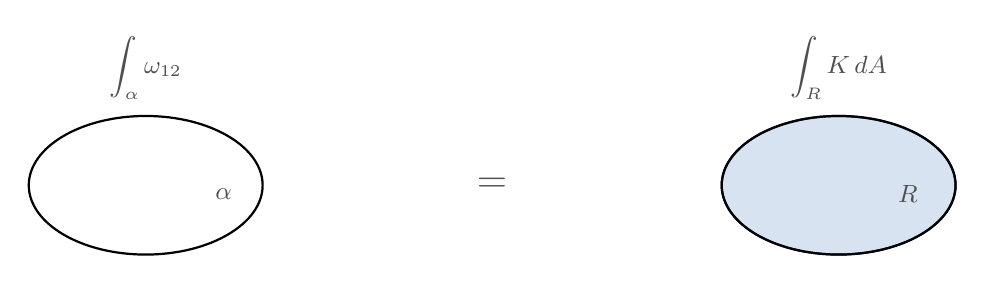
\begin{tikzpicture}[p10, scale=1.1]
		
		% Left: boundary integral
		\draw[p10loop, ->] (-4.0,0) ellipse [x radius=1.35, y radius=0.80];
		\node[p10note] at (-4.0,1.35) {$\displaystyle \int_{\alpha}\omega_{12}$};
		\node[p10note] at (-3.1,-0.1) {$\alpha$};
		
		% Equals
		\node[p10eq] at (0,0) {$=$};
		
		% Right: area integral
		\path[p10region, fill=P10Blue!18]
		(4.0,0) ellipse [x radius=1.35, y radius=0.80];
		\draw[p10loop] (4.0,0) ellipse [x radius=1.35, y radius=0.80];
		\node[p10note] at (4.0,1.35) {$\displaystyle \int_{R}K\,dA$};
		\node[p10note] at (4.8,-0.1) {$R$};
		
	\end{tikzpicture}
	\caption{Stokes + structure equation: $\int_{\alpha}\omega_{12}=\int_{R}K\,dA$.}
	\label{fig:p10-stokes-tikz}
\end{figure}
	
	
	% -------------------------------------------------
	% FIGURE 5: Sphere intuition --- area equals holonomy (K=1)
	% -------------------------------------------------
	\begin{figure}[htbp]
		\centering
		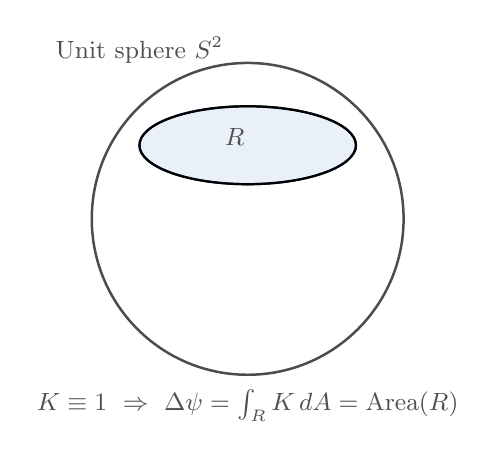
\begin{tikzpicture}[p10, scale=1.1]
			
			% Sphere outline (as circle)
			\draw[black!70, line width=0.9pt] (0,0) circle (1.8);
			\node[p10note] at (-1.25,1.95) {Unit sphere $S^2$};
			
			% A boundary curve (latitude-like) and cap region
			\path[p10region, fill=P10Blue!10]
			(0.0,0.85) ellipse [x radius=1.25, y radius=0.45];
			\draw[p10loop, ->] (0.0,0.85) ellipse [x radius=1.25, y radius=0.45];
			
			\node[p10note] at (-0.15,0.95) {$R$};
			
			% Annotation
			\node[p10note] at (0,-2.15)
			{$K\equiv 1 \ \Rightarrow\ \Delta\psi=\int_R K\,dA=\mathrm{Area}(R)$};
			
		\end{tikzpicture}
		\caption{On the unit sphere, curvature is constant \(K=1\), so holonomy equals enclosed area (with consistent orientation conventions).}
		\label{fig:p10-sphere-tikz}
	\end{figure}
	
	
	% -------------------------------------------------
	% FIGURE 6: Plane vs cylinder --- intrinsic vs extrinsic
	% -------------------------------------------------
	\begin{figure}[htbp]
		\centering
		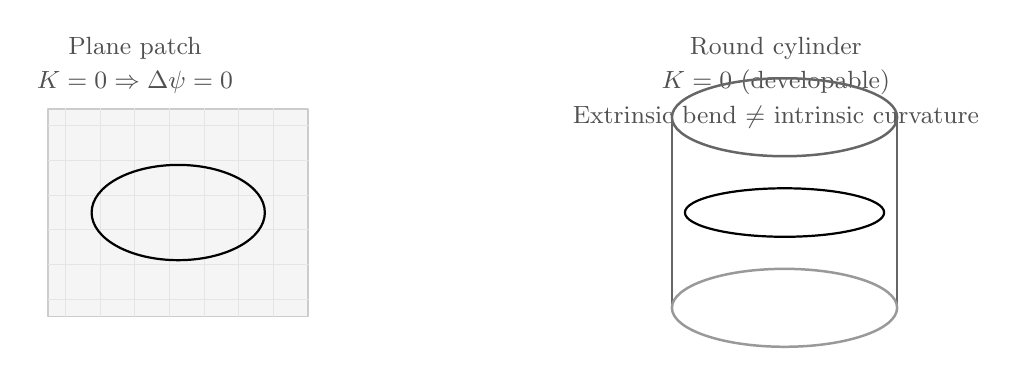
\begin{tikzpicture}[p10, scale=1.1]
			
			% --- Left: plane patch
			\node[p10note] at (-4.2,1.9) {Plane patch};
			\node[p10note] at (-4.2,1.5) {$K=0 \Rightarrow \Delta\psi=0$};
			
			% plane grid patch
			\path[fill=black!4, draw=black!20, line width=0.7pt] (-5.2,-1.2) rectangle (-2.2,1.2);
			\foreach \x in {-5.0,-4.6,...,-2.4}{
				\draw[black!10] (\x,-1.2) -- (\x,1.2);
			}
			\foreach \y in {-1.0,-0.6,...,1.0}{
				\draw[black!10] (-5.2,\y) -- (-2.2,\y);
			}
			
			% loop on plane
			\draw[p10loop, ->] (-3.7,0) ellipse [x radius=1.0, y radius=0.55];
			
			% --- Right: cylinder (schematic 3D)
			\node[p10note] at (3.2,1.9) {Round cylinder};
			\node[p10note] at (3.2,1.5) {$K=0$ (developable)};
			\node[p10note] at (3.2,1.1) {Extrinsic bend $\neq$ intrinsic curvature};
			
			% cylinder body
			\draw[black!60, line width=0.9pt] (2.0,-1.1) -- (2.0,1.1);
			\draw[black!60, line width=0.9pt] (4.6,-1.1) -- (4.6,1.1);
			\draw[black!60, line width=0.9pt] (3.3,1.1) ellipse [x radius=1.3, y radius=0.45];
			\draw[black!40, line width=0.9pt] (3.3,-1.1) ellipse [x radius=1.3, y radius=0.45];
			
			% loop around cylinder (mid ellipse)
			\draw[p10loop, ->] (3.3,0) ellipse [x radius=1.15, y radius=0.28];
			
		\end{tikzpicture}
		\caption{Both a plane and a round cylinder have \(K=0\). The cylinder is curved in \(\mathbb{R}^3\) but intrinsically flat, so small-loop holonomy is \(0\).}
		\label{fig:p10-dev-tikz}
	\end{figure}
	
	
	% -------------------------------------------------
	% FIGURE 7: Geodesic triangle and angle excess
	% -------------------------------------------------
	\begin{figure}[htbp]
		\centering
		\begin{tikzpicture}[p10, scale=1.15]
			
			% Surface blob (conceptual)
			\path[p10region, fill=P10Blue!08]
			(0,0) .. controls (1.6,1.0) and (3.2,0.9) .. (3.4,0)
			.. controls (3.5,-1.0) and (1.8,-1.25) .. (0.4,-0.8)
			.. controls (-0.5,-0.45) and (-0.4,0.6) .. cycle;
			
			\node[p10note] at (2.8,0.85) {Geodesic triangle};
			
			% Triangle vertices
			\coordinate (A) at (0.7,-0.3);
			\coordinate (B) at (2.9,-0.5);
			\coordinate (C) at (1.8,0.8);
			
			% "Geodesic" edges (slightly curved for visual)
			\draw[P10Blue!80!black, line width=1.0pt]
			(A) to[out=10,in=190] (B)
			(B) to[out=120,in=-20] (C)
			(C) to[out=-150,in=60] (A);
			
			\fill (A) circle (1.2pt) node[below left,p10note] {$A$};
			\fill (B) circle (1.2pt) node[below right,p10note] {$B$};
			\fill (C) circle (1.2pt) node[above,p10note] {$C$};
			
			% Angle labels without angles/quotes library
			\node[p10note, P10Red!80!black] at ($(A)+(0.30,0.18)$) {$\alpha$};
			\node[p10note, P10Red!80!black] at ($(B)+(-0.30,0.18)$) {$\beta$};
			\node[p10note, P10Red!80!black] at ($(C)+(0,-0.28)$) {$\gamma$};

			\node[p10note, align=left] at (-0.15,0.95)
			{Angle excess:\\
				$\alpha+\beta+\gamma-\pi = \displaystyle\int_R K\,dA$};
			
		\end{tikzpicture}
		\caption{Geodesic triangle viewpoint: curvature produces angle excess; the defect is the integral of \(K\) over the enclosed region.}
		\label{fig:p10-triangle-tikz}
	\end{figure}
\end{solution}

\section{Bundles and Forms}

\subsection*{Main-text correspondence: VII/07}

\begin{problem}[CP-VII-0028 --- Problem 8: The M\\"{o}bius line bundle and the tautological bundle on $\mathbb{RP}^1$]
\label{prob:cp-vii-0028}

\noindent Define the M\\"{o}bius bundle $M\to S^1$ to be the real line bundle trivialised over
\[
U_\pm \;=\; S^1\setminus\{(0,\pm 1)\},
\]
with transition function
\[
g_{+-}:\; U_+\cap U_- \;=\; S^1\setminus\{(0,\pm 1)\}\longrightarrow GL(1,\mathbb{R})=\mathbb{R}^\times
\]
given by $+1$ on the left-hand semicircle and $-1$ on the right-hand semicircle.
\begin{enumerate}
	\item[(a)] Show that $\mathbb{RP}^1$ is diffeomorphic to $S^1$.
	\item[(b)] Using this diffeomorphism to identify $\mathbb{RP}^1\cong S^1$, show that
	$M$ is isomorphic to the tautological bundle $\mathcal{O}_{\mathbb{RP}^1}(-1)$.
\end{enumerate}



\end{problem}

\begin{solution}

\par\medskip\noindent\textbf{(a) $\mathbb{RP}^1$ is diffeomorphic to $S^1$.}\par\smallskip

Write a point of $\mathbb{RP}^1$ as $[x:y]$ with $(x,y)\neq (0,0)$ and $[x:y]=[\lambda x:\lambda y]$
for $\lambda\neq 0$.
Define
\[
\Phi:\mathbb{RP}^1 \longrightarrow S^1\subset\mathbb{R}^2,\qquad
\Phi([x:y])=\left(\frac{x^2-y^2}{x^2+y^2},\,\frac{2xy}{x^2+y^2}\right).
\]
This is well-defined since the expression is homogeneous of degree $0$ in $(x,y)$.
Moreover,
\[
\left(\frac{x^2-y^2}{x^2+y^2}\right)^2+\left(\frac{2xy}{x^2+y^2}\right)^2
=\frac{(x^2+y^2)^2}{(x^2+y^2)^2}=1,
\]
so $\Phi([x:y])\in S^1$. If $(x,y)=(\cos\theta,\sin\theta)$ then
\[
\Phi([\cos\theta:\sin\theta])=(\cos 2\theta,\sin 2\theta),
\]
so $\Phi$ is the angle-doubling map, which is precisely invariant under $\theta\sim\theta+\pi$.

To write a smooth inverse, use two charts on $S^1$:
on $S^1\setminus\{(-1,0)\}$ (where $1+X\neq 0$) set
\[
\Psi_0(X,Y)=\left[\,1:\frac{Y}{1+X}\right],
\]
and on $S^1\setminus\{(1,0)\}$ (where $1-X\neq 0$) set
\[
\Psi_1(X,Y)=\left[\,\frac{Y}{1-X}:1\right].
\]
These definitions agree on the overlap and glue to a smooth inverse $\Psi:S^1\to \mathbb{RP}^1$.
Hence $\Phi$ is a diffeomorphism $\mathbb{RP}^1\cong S^1$.

\par\medskip\noindent\textbf{(b) $M \cong \mathcal{O}_{\mathbb{RP}^1}(-1)$.}\par\smallskip

Let $\gamma^1=\mathcal{O}_{\mathbb{RP}^1}(-1)$ be the tautological real line bundle
\[
\gamma^1=\{(\ell,v)\in\mathbb{RP}^1\times\mathbb{R}^2:\ v\in \ell\}\longrightarrow \mathbb{RP}^1.
\]
Transport $\gamma^1$ to a line bundle over $S^1$ via the diffeomorphism $\Phi$, i.e.\ consider
$\widetilde{\gamma}:=(\Phi^{-1})^*(\gamma^1)\to S^1$.

Real line bundles over $S^1$ are classified by $H^1(S^1;\mathbb{Z}_2)\cong \mathbb{Z}_2$:
there are exactly two isomorphism classes, the trivial line bundle and the unique nontrivial one (the M\\"{o}bius bundle).
The tautological bundle $\gamma^1$ over $\mathbb{RP}^1$ is nontrivial (equivalently $w_1(\gamma^1)\neq 0$),
hence $\widetilde{\gamma}$ is a nontrivial real line bundle over $S^1$.
Therefore $\widetilde{\gamma}$ is isomorphic to the M\\"{o}bius bundle $M$ determined by the transition
function $g_{+-}$, and thus (under $\mathbb{RP}^1\cong S^1$) one has
\[
M \;\cong\; \mathcal{O}_{\mathbb{RP}^1}(-1).
\]



% THEORY: Problems 8--10


% ------------------------------------------------------------
% Theory for Problem 8
% ------------------------------------------------------------
\par\medskip\noindent\textbf{Theory for Problem 8: M\\"{o}bius line bundle, $\mathbb{RP}^1 \cong S^1$, and $\mathcal{O}_{\mathbb{RP}^1}(-1)$}\par\smallskip


\par\medskip\noindent\textbf{(8.1) Real line bundles via transition functions.}\par\smallskip

A real line bundle $L\to X$ can be described by an open cover $\{U_i\}$ of $X$, local trivialisations
$L|_{U_i}\cong U_i\times \mathbb{R}$, and \emph{transition functions}
\[
g_{ij}:U_i\cap U_j \longrightarrow GL(1,\mathbb{R})=\mathbb{R}^\times
\]
satisfying $g_{ii}=1$ and the cocycle condition $g_{ij}\,g_{jk}=g_{ik}$ on triple overlaps.
Changing trivialisations multiplies $g_{ij}$ by a coboundary, so isomorphism classes of real line bundles
are governed by $H^1(X;\mathbb{Z}_2)$, via the first Stiefel--Whitney class $w_1(L)$.
Indeed, $\mathbb{R}^\times$ deformation retracts to $\{\pm 1\}$, so only the sign matters up to homotopy.

For $S^1$ one has
\[
H^1(S^1;\mathbb{Z}_2)\cong \mathbb{Z}_2,
\]
so there are exactly two real line bundles over $S^1$ up to isomorphism: the trivial bundle and the
nontrivial (M\\"{o}bius) bundle, distinguished by $w_1=0$ versus $w_1\neq 0$.

\par\medskip\noindent\textbf{(8.2) $\mathbb{RP}^1$ is a circle.}\par\smallskip

Recall $\mathbb{RP}^1$ is the space of lines through the origin in $\mathbb{R}^2$:
\[
\mathbb{RP}^1 \;=\; \bigl(\mathbb{R}^2\setminus\{0\}\bigr)/\sim,\qquad v\sim \lambda v\ (\lambda\neq 0).
\]
Equivalently, a line is determined by a unit vector $u\in S^1$ up to the identification $u\sim -u$, hence
\[
\mathbb{RP}^1 \cong S^1/\{\pm 1\}.
\]
Topologically this quotient is again a circle. Concretely, if $\theta$ is an angle coordinate on $S^1$,
then the projective identification corresponds to $\theta\sim \theta+\pi$, and the map
\[
[\theta]\in \mathbb{R}/(\pi\mathbb{Z}) \longmapsto e^{2i\theta}\in S^1
\]
is a smooth diffeomorphism $\mathbb{RP}^1\to S^1$.

\par\medskip\noindent\textbf{(8.3) The tautological bundle $\mathcal{O}_{\mathbb{RP}^1}(-1)$.}\par\smallskip

The tautological (universal) real line bundle over $\mathbb{RP}^1$ is
\[
\gamma^1 \;=\; \mathcal{O}_{\mathbb{RP}^1}(-1)
\;=\; \{(\ell,v)\in \mathbb{RP}^1\times \mathbb{R}^2:\ v\in \ell\}\longrightarrow \mathbb{RP}^1,
\]
whose fibre over a line $\ell$ is precisely the line $\ell\subset \mathbb{R}^2$.
This bundle is nontrivial: it represents the nonzero class in $H^1(\mathbb{RP}^1;\mathbb{Z}_2)$
(equivalently $w_1(\gamma^1)\neq 0$). Since $\mathbb{RP}^1\cong S^1$ and there is a unique nontrivial
real line bundle over $S^1$, it follows that under the identification $\mathbb{RP}^1\cong S^1$,
the tautological bundle $\mathcal{O}_{\mathbb{RP}^1}(-1)$ is isomorphic to the M\\"{o}bius bundle.



% Problem 9
\end{solution}

\begin{problem}[CP-VII-0029 --- Problem 9: Transition functions of $TS^2$ and identification with $\mathcal{O}_{\mathbb{CP}^1}(2)$]
\label{prob:cp-vii-0029}

\noindent Using the two standard stereographic projection charts, trivialise $TS^2$ over
\[
U_\pm \;=\; S^2\setminus\{(0,0,\pm 1)\},
\]
and calculate the transition function
\[
g_{+-}:\; U_+\cap U_- \longrightarrow GL(2,\mathbb{R}).
\]
Deduce that, as rank-$2$ real vector bundles,
\[
TS^2 \;\cong\; \mathcal{O}_{\mathbb{CP}^1}(2),
\]
i.e.\ viewing the fibres of $\mathcal{O}_{\mathbb{CP}^1}(2)$ as $\mathbb{R}^2$ instead of $\mathbb{C}$.



\end{problem}

\begin{solution}
Let $N=(0,0,1)$ and $S=(0,0,-1)$, and set
\[
U_+ = S^2\setminus\{N\},\qquad U_- = S^2\setminus\{S\}.
\]
Let $\phi_\pm:U_\pm\to \mathbb{R}^2\cong\mathbb{C}$ be the stereographic charts.
Using $\phi_\pm$, trivialise the tangent bundle by
\[
TS^2|_{U_\pm}\;\cong\; U_\pm\times \mathbb{R}^2,\qquad
v\in T_pS^2\longmapsto d(\phi_\pm)_p(v)\in \mathbb{R}^2.
\]
On the overlap $U_+\cap U_-$, the transition function is the Jacobian of the coordinate change:
\[
g_{+-}(p)=d\bigl(\phi_-\circ \phi_+^{-1}\bigr)\Big|_{\phi_+(p)}\in GL(2,\mathbb{R}).
\]

\par\medskip\noindent\textbf{(1) Computing $g_{+-}$.}\par\smallskip

With the standard stereographic conventions (and possibly composing one chart with complex conjugation),
the overlap map on $\mathbb{C}^\times$ can be written as
\[
w=\phi_-\circ\phi_+^{-1}(z)=\frac{1}{z},\qquad z\in\mathbb{C}^\times.
\]
Write $z=u+iv$ and $w=u'+iv'$. Then
\[
w=\frac{1}{u+iv}=\frac{u-iv}{u^2+v^2}
\quad\Longrightarrow\quad
(u',v')=\left(\frac{u}{u^2+v^2},\,-\frac{v}{u^2+v^2}\right).
\]
Let $\rho^2=u^2+v^2$. Differentiating gives
\[
D(u',v')
=
\frac{1}{\rho^4}
\begin{pmatrix}
	v^2-u^2 & -2uv\\
	2uv & v^2-u^2
\end{pmatrix}.
\]
Hence, in the chosen trivialisations,
\[
\boxed{
	g_{+-}(u,v)=
	\frac{1}{(u^2+v^2)^2}
	\begin{pmatrix}
		v^2-u^2 & -2uv\\
		2uv & v^2-u^2
	\end{pmatrix}
	\in GL(2,\mathbb{R}),\qquad (u,v)\neq(0,0).
}
\]
Equivalently, in complex notation, since $w=1/z$ one has
\[
dw=\left(-\frac{1}{z^2}\right)dz,
\]
so $g_{+-}$ is the real $2\times 2$ matrix representing multiplication by $-1/z^2$ on $\mathbb{C}\cong\mathbb{R}^2$
(the constant $-1$ can be absorbed by changing the frame on one chart).

\par\medskip\noindent\textbf{(2) Deduce $TS^2\cong \mathcal{O}_{\mathbb{CP}^1}(2)$ as real rank-$2$ bundles.}\par\smallskip

Under the identification $S^2\cong\mathbb{CP}^1$ (Riemann sphere), take affine coordinates
$z$ on $U_0=\{[1:z]\}$ and $w=1/z$ on $U_1=\{[w:1]\}$. Then the holomorphic tangent frames satisfy
\[
\frac{\partial}{\partial z}
=
\frac{dw}{dz}\frac{\partial}{\partial w}
=
\left(-\frac{1}{z^2}\right)\frac{\partial}{\partial w}.
\]
Thus the transition function of $T\mathbb{CP}^1$ is $-z^{-2}$, which agrees with that of $\mathcal{O}_{\mathbb{CP}^1}(2)$
up to the constant factor $-1$ (a gauge change). Therefore, as complex line bundles,
\[
T\mathbb{CP}^1 \cong \mathcal{O}_{\mathbb{CP}^1}(2).
\]
Viewing a complex line bundle as a real rank-$2$ bundle via $\mathbb{C}\cong\mathbb{R}^2$ yields
\[
TS^2 \;\cong\; \bigl(T\mathbb{CP}^1\bigr)_{\mathbb{R}}
\;\cong\; \bigl(\mathcal{O}_{\mathbb{CP}^1}(2)\bigr)_{\mathbb{R}},
\]
as required.


% ------------------------------------------------------------
% Theory for Problem 9
% ------------------------------------------------------------
\par\medskip\noindent\textbf{Theory for Problem 9: Transition functions of $TS^2$ and identification with $\mathcal{O}_{\mathbb{CP}^1}(2)$}\par\smallskip


\par\medskip\noindent\textbf{(9.1) Stereographic charts on $S^2$.}\par\smallskip

Let $S^2\subset \mathbb{R}^3$, and let $N=(0,0,1)$ and $S=(0,0,-1)$ be the north and south poles.
Define the standard cover
\[
U_+ = S^2\setminus\{N\},\qquad U_- = S^2\setminus\{S\}.
\]
Stereographic projection gives diffeomorphisms
\[
\phi_+:U_+\to \mathbb{R}^2 \cong \mathbb{C},\qquad
\phi_-:U_-\to \mathbb{R}^2 \cong \mathbb{C}.
\]
On the overlap $U_+\cap U_- = S^2\setminus\{N,S\}$, the coordinate change
\[
\phi_- \circ \phi_+^{-1}:\ \mathbb{C}^\times \longrightarrow \mathbb{C}^\times
\]
is (up to a convention) the inversion map
\[
w = \frac{1}{z}.
\]
This map is conformal; its complex derivative is $dw/dz = -1/z^2$.

\par\medskip\noindent\textbf{(9.2) Tangent bundle transition functions from Jacobians.}\par\smallskip

Given a chart $\phi:U\to \mathbb{R}^2$, a standard trivialisation of the tangent bundle over $U$ is
\[
TS^2|_U \cong U\times \mathbb{R}^2,\qquad
v\in T_pS^2 \mapsto (p,\, d\phi_p(v))\in U\times \mathbb{R}^2.
\]
Hence, on an overlap $U_+\cap U_-$ the transition function for $TS^2$ is given by the Jacobian matrix:
\[
g_{+-}(p)\;=\; d(\phi_- \circ \phi_+^{-1})\big|_{\phi_+(p)} \in GL(2,\mathbb{R}).
\]
Thus computing $g_{+-}$ reduces to differentiating the overlap map in local coordinates.

\par\medskip\noindent\textbf{(9.3) Why $\mathcal{O}_{\mathbb{CP}^1}(2)$ appears.}\par\smallskip

Using the identification $\mathbb{CP}^1\cong S^2$ (the Riemann sphere), one has the classical
holomorphic line bundle isomorphism
\[
T\mathbb{CP}^1 \cong \mathcal{O}_{\mathbb{CP}^1}(2).
\]
One way to see this is via the Euler sequence on $\mathbb{CP}^1$, or by the degree computation
$c_1(T\mathbb{CP}^1)=2$.
If we forget the complex structure, a complex line bundle becomes a real rank-$2$ vector bundle.
Thus, viewing fibres of $\mathcal{O}_{\mathbb{CP}^1}(2)$ as $\mathbb{R}^2$ rather than $\mathbb{C}$,
the statement $TS^2 \cong \mathcal{O}_{\mathbb{CP}^1}(2)$ is an identification of real rank-$2$ bundles.
At the level of transition functions: if $w=1/z$ on overlaps, then tangent vectors transform by
\[
\frac{\partial}{\partial z} = \frac{dw}{dz}\,\frac{\partial}{\partial w},\qquad \frac{dw}{dz}=-\frac{1}{z^2},
\]
which is precisely the $z^{-2}$ (degree $2$) behaviour encoded by $\mathcal{O}(2)$.



% Problem 10
\end{solution}

\subsection*{Main-text correspondence: VII/08}

\begin{problem}[CP-VII-0030 --- Local and global connection forms]
\label{prob:cp-vii-0030}
\begin{enumerate}[label=(\alph*)]
\item Let \(\pi:E\to B\) be a vector bundle and let
\[
A_\alpha\in\Omega^1\!\bigl(U_\alpha;\mathfrak{gl}(k,\mathbb R)\bigr)
\]
be local connection forms satisfying the preliminary compatibility condition.
Show that the resulting global
\(\mathfrak{gl}(k,\mathbb R)\)-valued \(1\)-form \(A\) is well defined on overlaps and satisfies the two defining conditions for a connection.
	\[
	\text{Hint: Show that}\quad
	D_\beta f_\alpha
	=
	(R_{g_{\beta\alpha}^{-1}})_*D_\alpha f_\alpha
	+
	f_\beta(b)\cdot\eta,
	\qquad
	\eta=g_{\beta\alpha}\,dg_{\beta\alpha}^{-1}\in\mathfrak{gl}(k,\mathbb{R}).
	\]
	\item Conversely show that if $A$ is a connection then the local forms $f_\alpha^*A$ satisfy the preliminary definition.
\end{enumerate}
\end{problem}

\begin{solution}
Let $P=\mathrm{Fr}(E)$ be the principal bundle of frames, with structure group
\[
G=\mathrm{GL}(k,\mathbb{R}).
\]
Let $\{U_\alpha\}$ be a trivializing cover with local sections (local frames)
\[
f_\alpha:U_\alpha\longrightarrow P.
\]
On overlaps $U_{\alpha\beta}=U_\alpha\cap U_\beta$, there are transition functions
\[
g_{\beta\alpha}:U_{\alpha\beta}\longrightarrow G
\]
such that
\[
f_\alpha(b)=f_\beta(b)\,g_{\beta\alpha}(b).
\]

\textbf{(a) Well-definedness and the connection axioms.}
Assume the preliminary definition, i.e. the local $1$-forms satisfy on overlaps
\[
A_\alpha
=
g_{\beta\alpha}\,A_\beta\,g_{\beta\alpha}^{-1}
+
g_{\beta\alpha}\,dg_{\beta\alpha}^{-1}.
\]
For $p\in P|_{U_\alpha}$ write uniquely
\[
p=f_\alpha(\pi(p))\cdot g_\alpha(p),
\qquad
g_\alpha(p)\in G.
\]
Define a $\mathfrak{gl}(k,\mathbb{R})$-valued $1$-form on $P|_{U_\alpha}$ by
\[
A
=
\mathrm{Ad}_{g_\alpha(p)^{-1}}\bigl(\pi^*A_\alpha\bigr)
+
g_\alpha^{-1}dg_\alpha.
\]
On an overlap, the factorization satisfies
\[
g_\beta(p)=g_{\beta\alpha}(\pi(p))\,g_\alpha(p).
\]
Using the overlap rule for $A_\alpha$ and the product rule for Maurer--Cartan forms,
\[
(g_{\beta\alpha}g_\alpha)^{-1}d(g_{\beta\alpha}g_\alpha)
=
g_\alpha^{-1}(g_{\beta\alpha}^{-1}dg_{\beta\alpha})g_\alpha
+
g_\alpha^{-1}dg_\alpha,
\]
one checks that the expression for $A$ obtained from $\alpha$ equals the one obtained from $\beta$. Hence $A$ is globally well-defined.

Moreover, $A$ satisfies the two connection axioms:
\[
R_h^*A=\mathrm{Ad}_{h^{-1}}A
\qquad\text{for all}\qquad
h\in G,
\]
and for every $\xi\in\mathfrak{g}$,
\[
A(\xi^\#)=\xi.
\]

\textbf{(b) Conversely, local forms from a global connection.}
Let $A$ be a connection form on $P$ and set
\[
A_\alpha:=f_\alpha^*A.
\]
On overlaps,
\[
f_\alpha=f_\beta\cdot g_{\beta\alpha},
\]
and using equivariance of $A$ together with the differential contribution from $dg_{\beta\alpha}$ (the hint term), one gets
\[
A_\alpha
=
g_{\beta\alpha}\,A_\beta\,g_{\beta\alpha}^{-1}
+
g_{\beta\alpha}\,dg_{\beta\alpha}^{-1}.
\]
Thus the $f_\alpha^*A$ satisfy the preliminary definition.
\end{solution}

\begin{problem}[CP-VII-0031 --- Problem 5 (Hopf bundle: local connection and curvature on $U_0$)]
\label{prob:cp-vii-0031}
Recall the connection we defined on the Hopf bundle
\[
S^{2n+1}\longrightarrow \mathbb{CP}^n
\]
via its horizontal distribution
\[
H_p \;=\; T_pS^{2n+1}\cap i\cdot T_pS^{2n+1}.
\]
Trivialise the bundle over $U_0\subset \mathbb{CP}^n$, and compute the local connection $1$-form $A$ and curvature $F$ in this trivialisation.
\end{problem}

\begin{solution}
Take the standard affine chart
\[
U_0 \;=\;\{[z_0:\cdots:z_n]\in \mathbb{CP}^n \;:\; z_0\neq 0\},
\]
with affine coordinates
\[
w_j \;=\;\frac{z_j}{z_0}\qquad (j=1,\dots,n).
\]
Define a local section $s_0:U_0\to S^{2n+1}\subset \mathbb{C}^{n+1}$ by
\[
s_0(w)\;=\;\frac{(1,w_1,\dots,w_n)}{\sqrt{1+\lVert w\rVert^2}},
\]
where
\[
\lVert w\rVert^2=\sum_{j=1}^n |w_j|^2.
\]
This yields a trivialisation
\[
U_0\times S^1 \longrightarrow \pi^{-1}(U_0),
\qquad
(w,e^{i\theta})\longmapsto e^{i\theta}\,s_0(w).
\]

On $S^{2n+1}$ take the standard Hopf connection $1$-form
\[
\alpha \;=\; -\,i\,\sum_{a=0}^n \overline{z_a}\,dz_a,
\]
whose kernel is exactly the horizontal distribution $H$.
In the above trivialisation one has
\[
\alpha \;=\; d\theta \;+\; A,
\]
where the local connection $1$-form on $U_0$ is
\[
A \;=\; s_0^{*}\alpha.
\]
A direct computation gives
\[
A \;=\; \frac{i}{2(1+\lVert w\rVert^2)}\sum_{j=1}^n\Bigl(w_j\,d\overline{w_j}-\overline{w_j}\,dw_j\Bigr).
\]
Equivalently,
\[
A \;=\; \operatorname{Im}\!\left(\frac{\sum_{j=1}^n \overline{w_j}\,dw_j}{1+\lVert w\rVert^2}\right).
\]

Since the structure group is abelian ($S^1$), the curvature is
\[
F \;=\; dA.
\]
Computing $dA$ yields
\[
F
\;=\;
\frac{i}{(1+\lVert w\rVert^2)^2}
\left(
(1+\lVert w\rVert^2)\sum_{j=1}^n dw_j\wedge d\overline{w_j}
\;-\;
\left(\sum_{j=1}^n \overline{w_j}\,dw_j\right)\wedge
\left(\sum_{k=1}^n w_k\,d\overline{w_k}\right)
\right).
\]

% -------------------------
% Problem 6
% -------------------------
\end{solution}

\subsection*{Main-text correspondence: VII/09}

\begin{problem}[CP-VII-0032 --- Problem 9(a) --- Harmonic forms are closed and coclosed]
\label{prob:cp-vii-0032}
Let $(X,g)$ be a compact oriented Riemannian $n$-manifold.
Show that a $p$-form $\alpha$ is harmonic if and only if it is closed and coclosed.
\textit{Hint:} for one direction consider $(\alpha,\Delta\alpha)_X$.
\end{problem}

\begin{solution}
Recall the Hodge Laplacian
\[
\Delta=d\delta+\delta d.
\]
On a compact manifold without boundary one has
\[
\langle \alpha,\Delta\alpha\rangle
=
\langle d\alpha,d\alpha\rangle
+
\langle \delta\alpha,\delta\alpha\rangle.
\]
If $\Delta\alpha=0$, then the left-hand side is $0$, so both norms vanish:
\[
d\alpha=0,
\]
\[
\delta\alpha=0.
\]
Conversely, if $d\alpha=0$ and $\delta\alpha=0$, then
\[
\Delta\alpha=d\delta\alpha+\delta d\alpha=0,
\]
so $\alpha$ is harmonic.
\end{solution}

\begin{problem}[CP-VII-0033 --- Problem 9(b) --- Poincar\'e duality via harmonic representatives]
\label{prob:cp-vii-0033}
By considering harmonic representatives, construct an isomorphism
\[
H^p_{\mathrm{dR}}(X)\to H^{n-p}_{\mathrm{dR}}(X)
\]
for each $p$.
\end{problem}

\begin{solution}
By the Hodge theorem, each class $[\omega]\in H^p_{\mathrm{dR}}(X)$ has a unique harmonic representative $\alpha$.
Define
\[
\Phi_p:H^p_{\mathrm{dR}}(X)\to H^{n-p}_{\mathrm{dR}}(X),
\]
\[
\Phi_p([\omega]):=[*\alpha].
\]
If $\alpha$ is harmonic, then $*\alpha$ is harmonic (equivalently $*$ commutes with $\Delta$), hence in particular closed:
\[
d(*\alpha)=0.
\]
Thus $[*\alpha]\in H^{n-p}_{\mathrm{dR}}(X)$.
Moreover,
\[
**\alpha=(-1)^{p(n-p)}\alpha,
\]
so $*$ is invertible on harmonic forms and $\Phi_p$ is an isomorphism.





\par\medskip\noindent\textbf{Theory for Problem 9 --- Hodge theory, harmonic forms, and Poincar\'e duality}\par\smallskip


On an oriented Riemannian $n$-manifold, the Hodge star is a map
\[
*:\Omega^p(X)\to\Omega^{n-p}(X),
\]
characterized by
\[
\alpha\wedge *\beta=\langle \alpha,\beta\rangle\,\mathrm{vol}_g.
\]
It satisfies
\[
**\alpha=(-1)^{p(n-p)}\alpha.
\]

The $L^2$ inner product on forms is
\[
(\alpha,\beta)=\int_X \langle \alpha,\beta\rangle\,\mathrm{vol}_g.
\]

The codifferential $\delta$ is the formal adjoint of $d$:
\[
(d\eta,\alpha)=(\eta,\delta\alpha).
\]
It can be written as
\[
\delta = (-1)^{n(p+1)+1}\,*\,d\,*
\]
on $p$-forms.

The Hodge Laplacian is
\[
\Delta=d\delta+\delta d.
\]
A form $\alpha$ is harmonic if
\[
\Delta\alpha=0.
\]
On a compact manifold without boundary one has the fundamental identity
\[
(\alpha,\Delta\alpha)=(d\alpha,d\alpha)+(\delta\alpha,\delta\alpha),
\]
so
\[
\Delta\alpha=0
\]
is equivalent to
\[
d\alpha=0,
\]
\[
\delta\alpha=0.
\]

Hodge decomposition states
\[
\Omega^p=\mathcal{H}^p\oplus d\Omega^{p-1}\oplus \delta\Omega^{p+1},
\]
and Hodge theorem identifies de Rham cohomology with harmonic forms:
\[
H^p_{\mathrm{dR}}(X)\cong \mathcal{H}^p.
\]
Moreover, $*$ maps harmonic forms to harmonic forms, hence induces an isomorphism
\[
H^p_{\mathrm{dR}}(X)\to H^{n-p}_{\mathrm{dR}}(X),
\]
given by
\[
[\alpha]\mapsto[*\alpha].
\]


\par\medskip\noindent\textbf{Extended theory for Problem 9 --- Hodge theory, harmonic forms, and duality}\par\smallskip


\textbf{Inner product and volume form.}
On an oriented Riemannian $n$-manifold $(X,g)$ one has a volume form $\mathrm{vol}_g$ and a pointwise inner product $\langle\cdot,\cdot\rangle$ on $p$-forms.
The global $L^2$ inner product is
\[
(\alpha,\beta)=\int_X \langle \alpha,\beta\rangle\,\mathrm{vol}_g.
\]

\textbf{Hodge star.}
The Hodge star is an isomorphism
\[
*:\Omega^p(X)\to\Omega^{n-p}(X),
\]
characterized by
\[
\alpha\wedge *\beta=\langle \alpha,\beta\rangle\,\mathrm{vol}_g.
\]
It satisfies
\[
**\alpha = (-1)^{p(n-p)}\alpha.
\]

\textbf{Codifferential.}
The codifferential $\delta:\Omega^p(X)\to\Omega^{p-1}(X)$ is defined by
\[
(d\eta,\alpha)=(\eta,\delta\alpha).
\]
It can be written as
\[
\delta = (-1)^{n(p+1)+1}\,*\,d\,*
\]
on $p$-forms.

\textbf{Closed and coclosed.}
A form $\alpha$ is closed if
\[
d\alpha=0.
\]
A form $\alpha$ is coclosed if
\[
\delta\alpha=0.
\]

\textbf{Hodge Laplacian and harmonic forms.}
The Hodge Laplacian is
\[
\Delta=d\delta+\delta d.
\]
A form $\alpha$ is harmonic if
\[
\Delta\alpha=0.
\]
On a compact manifold without boundary,
\[
(\alpha,\Delta\alpha)=(d\alpha,d\alpha)+(\delta\alpha,\delta\alpha).
\]
Thus
\[
\Delta\alpha=0
\]
is equivalent to
\[
d\alpha=0,
\]
\[
\delta\alpha=0.
\]

\textbf{Hodge decomposition and Hodge theorem.}
There is an orthogonal decomposition
\[
\Omega^p(X)=\mathcal{H}^p(X)\oplus d\Omega^{p-1}(X)\oplus \delta\Omega^{p+1}(X),
\]
where
\[
\mathcal{H}^p(X)=\{\alpha\in\Omega^p(X)\mid \Delta\alpha=0\}.
\]
Hodge theorem yields an isomorphism
\[
H^p_{\mathrm{dR}}(X)\cong \mathcal{H}^p(X),
\]
given by taking the unique harmonic representative of each class.

\textbf{Poincar\'e duality via $*$.}
The Hodge star maps harmonic forms to harmonic forms:
\[
\Delta\alpha=0
\quad\Longrightarrow\quad
\Delta(*\alpha)=0.
\]
Hence
\[
*:\mathcal{H}^p(X)\to\mathcal{H}^{n-p}(X)
\]
is an isomorphism, and therefore
\[
H^p_{\mathrm{dR}}(X)\cong H^{n-p}_{\mathrm{dR}}(X).
\]
\end{solution}

\begin{problem}[CP-VII-0034 --- Problem 11* --- div, grad, curl via $d$, $*$, and $\sharp/\flat$]
\label{prob:cp-vii-0034}
Consider $\mathbb{R}^3$ with its standard metric and orientation.
Express $\mathrm{div}$, $\mathrm{grad}$, and $\mathrm{curl}$ in terms of: the exterior derivative $d$, the Hodge star operator $*$, and raising and lowering indices.
\end{problem}

\begin{solution}
Let $\flat$ denote lowering indices and $\sharp$ denote raising indices.

\textit{Gradient.}
For a function $f$,
\[
\mathrm{grad}\,f=(df)^\sharp.
\]

\textit{Divergence.}
For a vector field $X$ with associated $1$-form $X^\flat$,
\[
\mathrm{div}\,X=*\,d\,*\,(X^\flat).
\]

\textit{Curl.}
For a vector field $X$,
\[
\mathrm{curl}\,X=\bigl(*\,d\,(X^\flat)\bigr)^\sharp.
\]


\par\medskip\noindent\textbf{Theory for Problem 11 --- Vector calculus via $d$, $*$, and $\sharp/\flat$}\par\smallskip


On $\mathbb{R}^3$ with Euclidean metric, lowering and raising indices are
\[
X^\flat=g(X,\cdot),
\]
\[
\alpha^\sharp \text{ is defined by } g(\alpha^\sharp,\cdot)=\alpha.
\]

For a function $f$,
\[
\mathrm{grad}\,f=(df)^\sharp.
\]
For a vector field $X$,
\[
\mathrm{curl}\,X=\bigl(*\,d\,(X^\flat)\bigr)^\sharp.
\]
For a vector field $X$,
\[
\mathrm{div}\,X=*\,d\,*\,(X^\flat).
\]

The codifferential satisfies (with standard sign conventions)
\[
\delta = (-1)^{n(p+1)+1}\,*\,d\,*.
\]
In particular, for $n=3$ and $p=1$,
\[
\delta=-*\,d\,*,
\]
so
\[
\mathrm{div}\,X=-\delta(X^\flat).
\]



\par\medskip\noindent\textbf{Extended theory for Problem 11 --- Vector calculus via differential forms in $\mathbb{R}^3$}\par\smallskip


\textbf{Musical isomorphisms.}
Using the Euclidean metric $g$,
\[
X^\flat=g(X,\cdot),
\]
\[
\alpha^\sharp \text{ is defined by } g(\alpha^\sharp,\cdot)=\alpha.
\]

\textbf{Vector calculus operators.}
For a function $f$,
\[
\mathrm{grad}\,f=(df)^\sharp.
\]
For a vector field $X$,
\[
\mathrm{curl}\,X=\bigl(*\,d\,(X^\flat)\bigr)^\sharp.
\]
For a vector field $X$,
\[
\mathrm{div}\,X=*\,d\,*\,(X^\flat).
\]

\textbf{Codifferential and divergence.}
The codifferential on $p$-forms is
\[
\delta = (-1)^{n(p+1)+1}\,*\,d\,*.
\]
For $n=3$ and $p=1$,
\[
\delta=-*\,d\,*,
\]
so
\[
\mathrm{div}\,X=-\delta(X^\flat).
\]

\textbf{Laplacian.}
The Hodge Laplacian is
\[
\Delta=d\delta+\delta d.
\]
For functions $f$,
\[
\Delta f=\delta df.
\]

\end{solution}

\subsection*{Main-text correspondence: VII/10}

\begin{problem}[CP-VII-0035 --- Antipodal map and orientability of \(\mathbb{RP}^n\)]
\label{prob:cp-vii-0035}
\begin{enumerate}
\item[(a)] For which \(n\) is the antipodal map
\[
\alpha:S^n\longrightarrow S^n
\]
orientation-preserving?

\item[(b)] Consider the natural two-to-one map
\[
\pi:S^n\longrightarrow\mathbb{RP}^n.
\]
Deduce for which \(n\) the manifold \(\mathbb{RP}^n\) is orientable.
You may assume that \(\pi\) is locally a diffeomorphism.

\item[(c)] Combining these ideas with Q5 and Q7, compute
\[
H^n_{\mathrm{dR}}(\mathbb{RP}^n)
\]
for all \(n\).
\end{enumerate}
	
	
	\textbf{Problem 8. Antipodal map, orientability of real projective space, and top de Rham cohomology}
\end{problem}

\begin{solution}
Let $\alpha:S^n\to S^n$ be the antipodal map $\alpha(x)=-x$.
	
	\textbf{(a)} Consider the linear map $-I:\mathbb{R}^{n+1}\to\mathbb{R}^{n+1}$. Its determinant is
	\[
	\det(-I)=(-1)^{n+1}.
	\]
	The antipodal map is the restriction of $-I$ to $S^n$, and its degree equals
	\[
	\deg(\alpha)=(-1)^{n+1}.
	\]
	A smooth map $S^n\to S^n$ is orientation-preserving iff its degree is $+1$. Hence $\alpha$ is orientation-preserving iff
	\[
	(-1)^{n+1}=+1 \quad \Longleftrightarrow \quad n \text{ is odd.}
	\]
	
	\textbf{(b)} Let $\pi:S^n\to \mathbb{RP}^n$ be the natural $2:1$ quotient map. We may assume $\pi$ is locally a diffeomorphism, hence a covering map. The nontrivial deck transformation is precisely the antipodal map $\alpha$.
	
	An orientation on $\mathbb{RP}^n$ pulls back via $\pi$ to an orientation on $S^n$; conversely, an orientation on $S^n$ descends to $\mathbb{RP}^n$ iff it is invariant under deck transformations. Therefore
	\[
	\mathbb{RP}^n \text{ is orientable}
	\;\Longleftrightarrow\;
	\alpha \text{ is orientation-preserving on } S^n
	\;\Longleftrightarrow\;
	n \text{ is odd.}
	\]
	
	\textbf{(c)} With real coefficients, torsion vanishes in cohomology. Also $\mathbb{RP}^n$ is connected, so
	\[
	H^0_{\mathrm{dR}}(\mathbb{RP}^n)\cong \mathbb{R}.
	\]
	For $0<k<n$, the (integral) cohomology of $\mathbb{RP}^n$ consists only of $2$-torsion, hence
	\[
	H^k_{\mathrm{dR}}(\mathbb{RP}^n)\cong 0 \qquad (0<k<n).
	\]
	Finally, the top de Rham cohomology satisfies
	\[
	H^n_{\mathrm{dR}}(\mathbb{RP}^n)\cong
	\begin{cases}
		\mathbb{R}, & \mathbb{RP}^n \text{ orientable},\\
		0, & \mathbb{RP}^n \text{ non-orientable},
	\end{cases}
	\]
	so using part (b),
	\[
	H^n_{\mathrm{dR}}(\mathbb{RP}^n)\cong
	\begin{cases}
		\mathbb{R}, & n \text{ odd},\\
		0, & n \text{ even}.
	\end{cases}
	\]
	Equivalently, for all $k$,
	\[
	H^k_{\mathrm{dR}}(\mathbb{RP}^n)\cong
	\begin{cases}
		\mathbb{R}, & k=0,\\
		0, & 0<k<n,\\
		\mathbb{R}, & k=n \text{ and } n \text{ odd},\\
		0, & k=n \text{ and } n \text{ even}.
	\end{cases}
	\]
	
		\textbf{Problem 8. Antipodal map, orientability of real projective space, and top de Rham cohomology}
	
	\textbf{Solution.}
	Let $\alpha:S^n\to S^n$ be the antipodal map $\alpha(x)=-x$.
	
	\textbf{(a)} The map $\alpha$ is the restriction to $S^n\subset\mathbb{R}^{n+1}$ of the linear map $-I$ on $\mathbb{R}^{n+1}$.
	Its determinant is
	\[
	\det(-I)=(-1)^{n+1}.
	\]
	The antipodal map has degree
	\[
	\deg(\alpha)=(-1)^{n+1}.
	\]
	A smooth map $S^n\to S^n$ is orientation-preserving iff its degree is $+1$. Hence
	\[
	\alpha \text{ is orientation-preserving}
	\iff (-1)^{n+1}=+1
	\iff n \text{ is odd.}
	\]
	
	\textbf{(b)} Let $\pi:S^n\to \mathbb{RP}^n$ be the natural $2:1$ quotient map. We may assume $\pi$ is locally a diffeomorphism, hence a covering map.
	The only nontrivial deck transformation is the antipodal map $\alpha$.
	
	An orientation on $\mathbb{RP}^n$ pulls back along $\pi$ to an orientation on $S^n$.
	Conversely, an orientation on $S^n$ descends to $\mathbb{RP}^n$ iff it is invariant under all deck transformations, i.e. iff $\alpha$ preserves orientation.
	Therefore
	\[
	\mathbb{RP}^n \text{ is orientable}
	\iff \alpha \text{ is orientation-preserving on } S^n
	\iff n \text{ is odd.}
	\]
	
	\textbf{(c)} Since $\mathbb{RP}^n$ is connected, we have
	\[
	H^0_{\mathrm{dR}}(\mathbb{RP}^n)\cong \mathbb{R}.
	\]
	For $0<k<n$, the (integral) cohomology of $\mathbb{RP}^n$ is $2$-torsion only, hence with real coefficients (and therefore in de Rham cohomology) it vanishes:
	\[
	H^k_{\mathrm{dR}}(\mathbb{RP}^n)=0 \qquad (0<k<n).
	\]
	Finally, for a closed connected $n$-manifold $M$,
	\[
	H^n_{\mathrm{dR}}(M)\cong
	\begin{cases}
		\mathbb{R}, & M \text{ orientable},\\
		0, & M \text{ non-orientable}.
	\end{cases}
	\]
	Using part (b), $\mathbb{RP}^n$ is orientable iff $n$ is odd, hence
	\[
	H^n_{\mathrm{dR}}(\mathbb{RP}^n)\cong
	\begin{cases}
		\mathbb{R}, & n \text{ odd},\\
		0, & n \text{ even}.
	\end{cases}
	\]
	Equivalently, for all $k$,
	\[
	H^k_{\mathrm{dR}}(\mathbb{RP}^n)\cong
	\begin{cases}
		\mathbb{R}, & k=0,\\
		0, & 0<k<n,\\
		\mathbb{R}, & k=n \text{ and } n \text{ odd},\\
		0, & k=n \text{ and } n \text{ even}.
	\end{cases}
	\]
\end{solution}

\begin{problem}[CP-VII-0036 --- Problem 10*. Hairy ball theorem via antipodal map and de Rham cohomology]
\label{prob:cp-vii-0036}
For even $n>2$ there is no nowhere-zero tangent vector field on $S^n$.
Prove this by:
(a) showing that a nowhere-zero tangent field on $S^n$ induces a homotopy from $\mathrm{id}_{S^n}$ to the antipodal map,
and (b) using de Rham cohomology to show that no such homotopy exists.
\end{problem}

\begin{solution}
\textbf{(a)} Assume there exists a nowhere-zero tangent vector field $V$ on $S^n$.
Define the normalized field
\[
U(x)=\frac{V(x)}{\|V(x)\|}\in T_xS^n.
\]
Since $U(x)\in T_xS^n$, we have $U(x)\cdot x=0$ in $\mathbb{R}^{n+1}$, and $\|U(x)\|=1$.

Define a map $H:S^n\times[0,1]\to S^n$ by
\[
H(x,t)=\cos(\pi t)\,x+\sin(\pi t)\,U(x).
\]
Because $x\perp U(x)$ and $\|x\|=\|U(x)\|=1$,
\[
\|H(x,t)\|^2=\cos^2(\pi t)\|x\|^2+\sin^2(\pi t)\|U(x)\|^2
=\cos^2(\pi t)+\sin^2(\pi t)=1,
\]
so $H(x,t)\in S^n$ for all $(x,t)$.
Moreover,
\[
H(x,0)=x \quad\text{and}\quad H(x,1)=\cos(\pi)x+\sin(\pi)U(x)=-x.
\]
Thus $H$ is a homotopy from $\mathrm{id}_{S^n}$ to the antipodal map $\alpha(x)=-x$.

\textbf{(b)} On $S^n$ we have $H^n_{\mathrm{dR}}(S^n)\cong \mathbb{R}$, generated by the cohomology class $[\omega]$
of any volume form $\omega$ with $\int_{S^n}\omega\neq 0$.
For a smooth map $f:S^n\to S^n$,
\[
f^*([\omega])=\deg(f)\,[\omega].
\]
In particular, homotopic maps induce the same map on de Rham cohomology, hence have the same degree.

Now $\deg(\mathrm{id}_{S^n})=1$, while the antipodal map $\alpha(x)=-x$ has degree
\[
\deg(\alpha)=(-1)^{n+1}.
\]
If $n$ is even, then $(-1)^{n+1}=-1$, so
\[
\alpha^*([\omega])=-[\omega]\neq [\omega]=\mathrm{id}^*([\omega]).
\]
Therefore $\mathrm{id}_{S^n}$ and $\alpha$ cannot be homotopic when $n$ is even.
This contradicts part (a), which produced a homotopy $\mathrm{id}_{S^n}\simeq \alpha$ from a nowhere-zero tangent field.

Hence no nowhere-zero tangent vector field on $S^n$ exists for even $n>2$.

\medskip
\textbf{Examples.}
For odd spheres $S^{2m+1}\subset \mathbb{C}^{m+1}$, the vector field $V(z)=iz$ is tangent and nowhere zero, so odd spheres admit
nowhere-zero tangent vector fields, in contrast to the even-dimensional case.
\end{solution}

\subsection*{Main-text correspondence: VII/11}

\begin{problem}[CP-VII-0037 --- Problem 9: Green's theorem via Stokes' theorem (pullback of a 1-form)]
\label{prob:cp-vii-0037}
Let $\Sigma$ be a compact $2$-manifold-with-boundary, let $F : \Sigma \to \mathbb{R}^2$ be a smooth map,
	and let $\alpha$ be the $1$-form $P\,dx + Q\,dy$ on $\mathbb{R}^2$ (where $P$ and $Q$ are smooth functions).
	Prove a version of Green's theorem by applying Stokes to $F^{*}\alpha$.
	
	
	\bigskip
	\textbf{Problem 9. Green's theorem via Stokes' theorem (pullback of a $1$-form)}
\end{problem}

\begin{solution}
Let $\Sigma$ be a compact oriented $2$-manifold with boundary, let $F:\Sigma\to\mathbb{R}^2$ be smooth, and let
	\[
	\alpha = P\,dx + Q\,dy
	\]
	be a $1$-form on $\mathbb{R}^2$, where $P,Q$ are smooth functions.
	
	Apply Stokes' theorem to the pulled-back $1$-form $F^*\alpha$ on $\Sigma$:
	\[
	\int_{\partial\Sigma} F^*\alpha
	=
	\int_{\Sigma} d(F^*\alpha).
	\]
	Using naturality of the exterior derivative ($d\circ F^* = F^*\circ d$), we get
	\[
	\int_{\partial\Sigma} F^*\alpha
	=
	\int_{\Sigma} F^*(d\alpha).
	\]
	
	Now compute $d\alpha$. Since $d(dx)=d(dy)=0$,
	\[
	d\alpha = d(P\,dx)+d(Q\,dy)= dP\wedge dx + dQ\wedge dy.
	\]
	Writing $dP=P_x\,dx+P_y\,dy$ and $dQ=Q_x\,dx+Q_y\,dy$, we obtain
	\[
	dP\wedge dx = (P_x\,dx+P_y\,dy)\wedge dx = P_y\,dy\wedge dx = -P_y\,dx\wedge dy,
	\]
	\[
	dQ\wedge dy = (Q_x\,dx+Q_y\,dy)\wedge dy = Q_x\,dx\wedge dy,
	\]
	hence
	\[
	d\alpha = (Q_x - P_y)\,dx\wedge dy
	=
	\left(\frac{\partial Q}{\partial x}-\frac{\partial P}{\partial y}\right)\,dx\wedge dy.
	\]
	
	Write $F=(u,v)$, where $u=x\circ F$ and $v=y\circ F$. Then $F^*(dx)=du$, $F^*(dy)=dv$, and therefore
	\[
	F^*(dx\wedge dy)=du\wedge dv.
	\]
	Also,
	\[
	F^*\alpha = (P\circ F)\,du + (Q\circ F)\,dv.
	\]
	Putting everything together gives the Green/Stokes identity:
	\[
	\int_{\partial\Sigma}\Big( (P\circ F)\,du + (Q\circ F)\,dv\Big)
	=
	\int_{\Sigma}
	\Big(\big(\tfrac{\partial Q}{\partial x}-\tfrac{\partial P}{\partial y}\big)\circ F\Big)\,du\wedge dv.
	\]
	When $\Sigma\subset\mathbb{R}^2$ and $F$ is the inclusion map, this reduces to the classical Green's theorem.
\end{solution}

\subsection*{Main-text correspondence: VII/21}

\begin{problem}[CP-VII-0038 --- Problem 11 (Coset foliations and integrability of left-invariant distributions)]
\label{prob:cp-vii-0038}
Let $G$ be a Lie group. Given an embedded Lie subgroup $H$, show that its left cosets induce a foliation of $G$,
with tangent distribution $\{\xi^L:\xi\in\mathfrak h\}$.
Given instead a subspace $\mathfrak h$ of $\mathfrak g$, show that the distribution $\{\xi^L:\xi\in\mathfrak h\}$
on $G$ arises from a foliation iff $\mathfrak h$ is actually a Lie subalgebra of $\mathfrak g$, i.e.\ $\mathfrak h$
is closed under the Lie bracket on $\mathfrak g$.
If this holds, must $\mathfrak h$ be the Lie algebra of an embedded subgroup of $G$?
\end{problem}

\begin{solution}
\emph{Cosets give a foliation.}
For each $g\in G$, the left coset $gH$ is the image of $H$ under the diffeomorphism $L_g$, hence an embedded submanifold.
The cosets partition $G$ and locally define a foliation (equivalently, the quotient map $G\to G/H$ is a submersion when $H$
is embedded). At $gh\in gH$,
\[
T_{gh}(gH)=(dL_g)_h(T_hH)=(dL_{gh})_e(\mathfrak h)=\{\xi^L_{gh}:\xi\in\mathfrak h\}.
\]
Thus the tangent distribution is $\mathcal D_p=\{\xi^L_p:\xi\in\mathfrak h\}$.

\emph{Integrability $\Longleftrightarrow$ $\mathfrak h$ is a Lie subalgebra.}
Given a vector subspace $\mathfrak h\subset\mathfrak g$, define a left-invariant distribution
\[
\mathcal D_g:=(dL_g)_e(\mathfrak h)=\{\xi^L_g:\xi\in\mathfrak h\}.
\]
By Frobenius, $\mathcal D$ arises from a foliation iff it is involutive.
Since $\mathcal D$ is spanned by left-invariant fields $\xi^L$ with $\xi\in\mathfrak h$, involutivity is equivalent to
\[
[\xi^L,\eta^L]\in\Gamma(\mathcal D)\quad\text{for all }\xi,\eta\in\mathfrak h.
\]
But $[\xi^L,\eta^L]=[\xi,\eta]^L$, so this holds iff $[\xi,\eta]\in\mathfrak h$ for all $\xi,\eta\in\mathfrak h$,
i.e.\ iff $\mathfrak h$ is a Lie subalgebra of $\mathfrak g$.

\emph{Embeddedness need not hold.}
If $\mathfrak h$ is a Lie subalgebra, it integrates to a unique connected \emph{immersed} Lie subgroup with Lie algebra
$\mathfrak h$, but it need not be embedded (equivalently, it need not be closed in $G$).
For example, in $G=\mathbb T^2=\mathbb R^2/\mathbb Z^2$ take $\mathfrak h=\mathrm{span}\{(1,\alpha)\}$ with
$\alpha\notin\mathbb Q$. The corresponding connected subgroup is dense in $\mathbb T^2$, hence not an embedded submanifold.
Thus $\mathfrak h$ need not be the Lie algebra of an embedded subgroup unless the integral subgroup is closed.

\par\medskip\noindent\textbf{Theory for Problem 11 (Maurer--Cartan form and structure equations)}\par\smallskip


\textbf{Left translation.}
For a Lie group $G$, left translation $L_g(h)=gh$ induces isomorphisms
\[
(dL_g)_e:\mathfrak g=T_eG \xrightarrow{\cong} T_gG.
\]
Hence $(dL_{g^{-1}})_g:T_gG\to\mathfrak g$ identifies each tangent space with the Lie algebra.

\textbf{Maurer--Cartan form.}
The (left) Maurer--Cartan form is the $\mathfrak g$-valued $1$-form
\[
\theta\in\Omega^1(G;\mathfrak g),\qquad \theta_g:=(dL_{g^{-1}})_g:T_gG\to\mathfrak g.
\]
It satisfies $(L_h)^*\theta=\theta$ and $\theta_e=\mathrm{id}_{\mathfrak g}$.
For matrix groups, $\theta=g^{-1}dg$.

\textbf{Left-invariant 1-forms.}
A $1$-form $\alpha$ is left-invariant if $(L_h)^*\alpha=\alpha$ for all $h$.
Left-invariant $1$-forms correspond to $\mathfrak g^*$ via
$\alpha_g(v)=\lambda(\theta_g(v))$ for $\lambda\in\mathfrak g^*$.

\textbf{Structure constants and components.}
Choose a basis $\{e_i\}$ of $\mathfrak g$ and dual left-invariant forms $\{\omega^i\}$.
If $[e_i,e_j]=\sum_k c_{ij}^k e_k$, then
\[
d\omega^k=-\frac12\sum_{i,j} c_{ij}^k\,\omega^i\wedge\omega^j.
\]

\textbf{Maurer--Cartan equation.}
In $\mathfrak g$-valued form,
\[
d\theta+\tfrac12[\theta,\theta]=0.
\]
Equivalently, for left-invariant vector fields $X,Y$,
\[
d\omega(X,Y)=-\omega([X,Y]).
\]

\textbf{Right translations and Ad.}
Often one uses $(R_h)^*\theta=\mathrm{Ad}_{h^{-1}}\theta$ to relate left/right invariance.
\end{solution}

\subsection*{Main-text correspondence: VII/22}

\begin{problem}[CP-VII-0039 --- Problem 10* --- Induced Levi--Civita connection on a submanifold]
\label{prob:cp-vii-0039}
Let $(X,g_X)$ be a Riemannian manifold and $\iota:Y\hookrightarrow X$ an embedded submanifold equipped with the metric
\[
g_Y=\iota^*g_X.
\]
Let $\nabla_X$ be the Levi--Civita connection on $X$, and let $\nabla_Y$ be the connection on $Y$ induced from $\nabla_X$ by the splitting
\[
\iota^*TX = TY \oplus TY^\perp.
\]
Show that $\nabla_Y$ is torsion-free and compatible with $g_Y$, and hence is the Levi--Civita connection on $Y$.
\end{problem}

\begin{solution}
Define the induced connection by tangential projection:
\[
\nabla^Y_U V := \bigl(\nabla^X_U V\bigr)^{\top},
\]
where $(\cdot)^\top$ denotes orthogonal projection to $TY$ in the splitting $TX|_Y=TY\oplus TY^\perp$.

\textit{Metric compatibility.}
For tangent fields $U,V,W$ on $Y$,
\[
U\langle V,W\rangle_Y
=
U\langle V,W\rangle_X.
\]
Using $\nabla^X g_X=0$ we have
\[
U\langle V,W\rangle_X
=
\langle \nabla^X_U V, W\rangle_X
+
\langle V,\nabla^X_U W\rangle_X.
\]
Since $W$ is tangent, it is orthogonal to normal components, hence
\[
\langle \nabla^X_U V, W\rangle_X
=
\langle (\nabla^X_U V)^\top, W\rangle_X
=
\langle \nabla^Y_U V, W\rangle_Y,
\]
and similarly
\[
\langle V,\nabla^X_U W\rangle_X
=
\langle V,(\nabla^X_U W)^\top\rangle_X
=
\langle V,\nabla^Y_U W\rangle_Y.
\]
Therefore
\[
U\langle V,W\rangle_Y
=
\langle \nabla^Y_U V, W\rangle_Y
+
\langle V,\nabla^Y_U W\rangle_Y,
\]
so $\nabla^Y$ is compatible with $g_Y$.

\textit{Torsion-freeness.}
The torsion of $\nabla^Y$ is
\[
T^Y(U,V)=\nabla^Y_U V-\nabla^Y_V U-[U,V].
\]
Because $\nabla^Y$ is tangential projection,
\[
\nabla^Y_U V-\nabla^Y_V U
=
\bigl(\nabla^X_U V-\nabla^X_V U\bigr)^\top.
\]
Since $\nabla^X$ is torsion-free,
\[
\nabla^X_U V-\nabla^X_V U=[U,V].
\]
Because $[U,V]$ is tangent to $Y$, projecting does nothing, so
\[
\bigl(\nabla^X_U V-\nabla^X_V U\bigr)^\top
=
[U,V].
\]
Hence
\[
T^Y(U,V)=0.
\]
Thus $\nabla^Y$ is torsion-free and metric-compatible, so by uniqueness it is the Levi--Civita connection of $(Y,g_Y)$.




\par\medskip\noindent\textbf{Theory for Problem 10 --- Induced connection on a submanifold}\par\smallskip


If $\iota:Y\hookrightarrow X$ is an embedded submanifold and
\[
g_Y=\iota^*g_X,
\]
then at each point $y\in Y$ there is an orthogonal splitting
\[
T_yX=T_yY\oplus (T_yY)^\perp.
\]
For the Levi--Civita connection $\nabla^X$ on $X$, the induced connection on $Y$ is defined by tangential projection:
\[
\nabla^Y_U V=\bigl(\nabla^X_U V\bigr)^\top.
\]
The normal component defines the second fundamental form:
\[
\mathrm{II}(U,V)=\bigl(\nabla^X_U V\bigr)^\perp.
\]
Thus one has the Gauss formula
\[
\nabla^X_U V=\nabla^Y_U V+\mathrm{II}(U,V).
\]

Metric compatibility follows from $\nabla^X g_X=0$ together with orthogonality of tangent and normal parts, yielding
\[
\nabla^Y g_Y=0.
\]
Torsion-freeness follows from torsion-freeness of $\nabla^X$ and tangency of Lie brackets:
\[
T^Y(U,V)=\nabla^Y_U V-\nabla^Y_V U-[U,V]=0.
\]
By uniqueness, $\nabla^Y$ is the Levi--Civita connection of $(Y,g_Y)$.


\par\medskip\noindent\textbf{Extended theory for Problem 10 --- Submanifolds, induced connection, and second fundamental form}\par\smallskip


\textbf{Induced metric.}
If $\iota:Y\hookrightarrow X$ is an embedded submanifold, define the induced metric by
\[
g_Y=\iota^*g_X.
\]

\textbf{Orthogonal splitting.}
For each $y\in Y$ there is an orthogonal decomposition
\[
T_yX=T_yY\oplus (T_yY)^\perp.
\]
Write $(\cdot)^\top$ and $(\cdot)^\perp$ for tangential and normal projections.

\textbf{Induced connection.}
Let $\nabla^X$ be the Levi--Civita connection on $(X,g_X)$.
For tangent fields $U,V$ on $Y$ define
\[
\nabla^Y_U V=\bigl(\nabla^X_U V\bigr)^\top.
\]

\textbf{Gauss formula and second fundamental form.}
Decompose $\nabla^X_U V$ into tangent and normal parts:
\[
\nabla^X_U V=\nabla^Y_U V+\mathrm{II}(U,V),
\]
where
\[
\mathrm{II}(U,V)=\bigl(\nabla^X_U V\bigr)^\perp
\]
is the second fundamental form.

\textbf{Levi--Civita property on $Y$.}
Metric compatibility descends from $X$:
\[
\nabla^X g_X=0
\quad\Longrightarrow\quad
\nabla^Y g_Y=0.
\]
Torsion-freeness also descends:
\[
T^X=0
\quad\Longrightarrow\quad
T^Y=0.
\]
Therefore $\nabla^Y$ is torsion-free and metric-compatible, hence it is the Levi--Civita connection on $(Y,g_Y)$.
\end{solution}

\section{Curves and Surfaces}

\subsection*{Main-text correspondence: VII/12}

\begin{problem}[CP-VII-0040 --- Arc-length reparametrization of a regular curve]
\label{prob:cp-vii-0040}
Let \(\gamma:(a,b)\to\mathbb R^m\) be a \(C^1\) regular curve, so
\(\gamma'(t)\neq0\) for every \(t\). Fix \(t_0\in(a,b)\) and define
\[
s(t)=\int_{t_0}^{t}\|\gamma'(u)\|\,du.
\]

\begin{enumerate}
\item Show that \(s'(t)>0\), hence \(s\) is locally invertible.
\item If \(t=t(s)\) denotes its inverse, define
\[
\widetilde\gamma(s)=\gamma(t(s)).
\]
Prove that \(\widetilde\gamma\) has unit speed.
\item Explain why arc length is therefore an intrinsic parameter along every
regular curve, unique up to translation and reversal of orientation.
\end{enumerate}
\end{problem}

\begin{solution}
The fundamental theorem of calculus gives
\[
s'(t)=\|\gamma'(t)\|>0.
\]
Hence \(s\) is strictly increasing and, by the inverse function theorem,
admits a \(C^1\) local inverse \(t=t(s)\).

By the chain rule,
\[
\frac{d\widetilde\gamma}{ds}
=
\gamma'(t(s))\frac{dt}{ds}.
\]
Since
\[
\frac{ds}{dt}=\|\gamma'(t)\|,
\qquad
\frac{dt}{ds}=\frac1{\|\gamma'(t)\|},
\]
we get
\[
\left\|\frac{d\widetilde\gamma}{ds}\right\|
=
\|\gamma'(t(s))\|
\frac1{\|\gamma'(t(s))\|}
=1.
\]
Thus \(\widetilde\gamma\) is unit-speed. Changing the reference point
\(t_0\) adds a constant to \(s\), while reversing orientation replaces
\(s\) by \(-s\) up to an additive constant.
\end{solution}

\subsection*{Main-text correspondence: VII/13}

\begin{problem}[CP-VII-0041 --- Problem 2]
\label{prob:cp-vii-0041}
Let $\alpha:I\to\mathbb{R}^3$ be a curve parametrized by arc length with $\tau(s)\neq 0$ and $\dot{k}(s)\neq 0$
	for all $s\in I$. Show that a necessary and sufficient condition for $\alpha(I)$ to lie on a sphere is that
	\[
	R^2 + (R')^2 T^2
	\quad\text{is constant,}
	\]
	where $R=1/k$ and $T=1/\tau$.
	
	\par\medskip\noindent\textbf{Theory (for Problems 2--3)}\par\smallskip

	Assume $\alpha$ is unit speed, so $T=\alpha'$ and $|T|=1$. If $k(s)\neq 0$, define
	\[
	k(s)=|\alpha''(s)|,\qquad N(s)=\frac{\alpha''(s)}{k(s)},\qquad B(s)=T(s)\times N(s).
	\]
	The Frenet--Serret formulas are
	\[
	T'=kN,\qquad N'=-kT+\tau B,\qquad B'=-\tau N.
	\]
	In particular, if $R=1/k$, then $k=1/R$.
\end{problem}

\begin{solution}
\noindent\textbf{Necessity.}
	Assume $\alpha(I)$ lies on a sphere. After translating the curve, we may assume the sphere is centered at the origin,
	so $|\alpha(s)|=\rho$ is constant. Differentiating $|\alpha|^2=\rho^2$ gives
	\[
	0=(|\alpha|^2)'=2\langle \alpha,\alpha'\rangle
	\quad\Longrightarrow\quad
	\langle \alpha,T\rangle=0.
	\]
	Differentiate $\langle \alpha,T\rangle=0$:
	\[
	0=\langle T,T\rangle+\langle \alpha,T'\rangle
	=1+\langle \alpha,kN\rangle
	\quad\Longrightarrow\quad
	\langle \alpha,N\rangle=-\frac{1}{k}=-R.
	\]
	Differentiate $\langle \alpha,N\rangle=-R$:
	\[
	-R'=\langle T,N\rangle+\langle \alpha,N'\rangle
	=\langle \alpha,-kT+\tau B\rangle
	=\tau\langle \alpha,B\rangle,
	\]
	using $\langle \alpha,T\rangle=0$. Hence
	\[
	\langle \alpha,B\rangle=-\frac{R'}{\tau}.
	\]
	Now decompose $\alpha$ in the orthonormal basis $(T,N,B)$:
	\[
	|\alpha|^2=\langle \alpha,T\rangle^2+\langle \alpha,N\rangle^2+\langle \alpha,B\rangle^2
	=0+R^2+\left(\frac{R'}{\tau}\right)^2
	=R^2+(R')^2T^2.
	\]
	Since $|\alpha|^2=\rho^2$ is constant, the expression $R^2+(R')^2T^2$ is constant.
	
	\medskip
	\noindent\textbf{Sufficiency.}
	Assume
	\[
	Q:=R^2+\left(\frac{R'}{\tau}\right)^2
	\quad\text{is constant.}
	\]
	Define
	\[
	c(s):=\alpha(s)+R(s)N(s)+\frac{R'(s)}{\tau(s)}\,B(s).
	\]
	Differentiate using Frenet--Serret:
	\[
	c' = T + R'N + R N' + \left(\frac{R'}{\tau}\right)'B + \frac{R'}{\tau}B'.
	\]
	Since $N'=-kT+\tau B=-(1/R)T+\tau B$ and $B'=-\tau N$, we obtain
	\[
	c' = T + R'N + R\left(-\frac1R T + \tau B\right) + \left(\frac{R'}{\tau}\right)'B + \frac{R'}{\tau}(-\tau N).
	\]
	The $T$-terms cancel and the $N$-terms cancel, leaving
	\[
	c'=\left(R\tau+\left(\frac{R'}{\tau}\right)'\right)B.
	\]
	Because $Q$ is constant,
	\[
	0=Q' = 2RR' + 2\frac{R'}{\tau}\left(\frac{R'}{\tau}\right)'.
	\]
	Since $\dot{k}\neq 0$, we have $R'=-k'/k^2\neq 0$, hence $R'/\tau\neq 0$, and we can divide to get
	\[
	\left(\frac{R'}{\tau}\right)'=-R\tau.
	\]
	Therefore $c'=0$, so $c(s)\equiv c_0$ is constant. Finally,
	\[
	|\alpha(s)-c_0|^2
	=\left|R N + \frac{R'}{\tau}B\right|^2
	=R^2+\left(\frac{R'}{\tau}\right)^2
	=Q,
	\]
	which is constant. Hence $\alpha(I)$ lies on the sphere centered at $c_0$ of radius $\sqrt{Q}$.
\end{solution}

\begin{problem}[CP-VII-0042 --- Problem 11 (Curvature and torsion of a helix; consequences for closed curves)]
\label{prob:cp-vii-0042}
If $a>0$, calculate the curvature and torsion of the smooth curve
	\[
	\alpha(s)=\bigl(a\cos(s/c),\,a\sin(s/c),\,bs/c\bigr),
	\qquad c=\sqrt{a^2+b^2}.
	\]
	Suppose now that $\alpha:[0,2\pi]\to\mathbb{R}^3$ is a smooth simple closed curve parametrized by arc-length
	with curvature everywhere positive.
	\begin{itemize}
		\item If both $\kappa$ and $\tau$ are constant, show that $\kappa=1$ and $\tau=0$.
		\item If $\kappa$ is constant and $\tau$ is not identically zero, show that $\kappa>1$.
		\item If $\alpha$ is knotted and $\tau$ is constant, show that $\kappa(s)>2$ for some $s\in[0,2\pi]$.
	\end{itemize}
\end{problem}

\begin{solution}
\textbf{(A) The helix $\alpha(s)=(a\cos(s/c),a\sin(s/c),bs/c)$.}
	Let $t=s/c$. Then $\alpha(s)=(a\cos t,a\sin t,bt)$ and $dt/ds=1/c$.
	Compute
	\[
	\alpha'(s)=\frac{1}{c}\,(-a\sin t,\,a\cos t,\,b),
	\qquad
	\|\alpha'(s)\|^2=\frac{1}{c^2}(a^2+b^2)=1,
	\]
	so $s$ is arc-length. Next,
	\[
	\alpha''(s)=\frac{1}{c^2}\,(-a\cos t,\,-a\sin t,\,0),
	\qquad
	\|\alpha''(s)\|=\frac{a}{c^2}.
	\]
	For a unit-speed curve, $\kappa=\|\alpha''\|$, hence
	\[
	\boxed{\ \kappa=\dfrac{a}{c^2}=\dfrac{a}{a^2+b^2}\ }.
	\]
	To find $\tau$, use the standard unit-speed formula
	\[
	\tau=\frac{\det(\alpha',\alpha'',\alpha''')}{\|\alpha'\times \alpha''\|^2}.
	\]
	A direct computation gives $\|\alpha'\times\alpha''\|^2=\kappa^2$ and
	$\det(\alpha',\alpha'',\alpha''')=\dfrac{ab}{c^6}$, hence
	\[
	\boxed{\ \tau=\dfrac{b}{c^2}=\dfrac{b}{a^2+b^2}\ }.
	\]
	(Equivalently: a circular helix has constant curvature $a/(a^2+b^2)$ and constant torsion $b/(a^2+b^2)$.)
	
	\medskip
	
	\textbf{(B) Closed unit-speed curves of length $2\pi$ with positive curvature.}
	
	\textbf{(B1) If $\kappa$ and $\tau$ are constant, then $\kappa=1$ and $\tau=0$.}
	A unit-speed curve with constant curvature $\kappa>0$ and constant torsion $\tau$ is, up to rigid motion,
	either a circle (if $\tau=0$) or a circular helix (if $\tau\neq 0$).
	But a circular helix is not closed unless $\tau=0$ (it has nonzero drift along its axis),
	so closedness forces $\tau=0$.
	
	Thus $\alpha$ is a circle of radius $1/\kappa$, hence its length is
	\[
	L=\frac{2\pi}{\kappa}.
	\]
	Since $\alpha$ is parametrized on $[0,2\pi]$ by arc-length, $L=2\pi$, so $\kappa=1$.
	Therefore $\tau=0$ and $\kappa=1$.
	
	\medskip
	
	\textbf{(B2) If $\kappa$ is constant and $\tau\not\equiv 0$, then $\kappa>1$.}
	By Fenchel's theorem (total curvature),
	\[
	\int_0^{2\pi} \kappa(s)\,ds \;\ge\; 2\pi,
	\]
	with equality if and only if the curve is a convex planar curve.
	Here $\kappa$ is constant and $L=2\pi$, so the left-hand side is
	\[
	\int_0^{2\pi}\kappa\,ds = \kappa\cdot 2\pi.
	\]
	Hence $\kappa\ge 1$.
	If $\tau\not\equiv 0$, then the curve is not planar, so equality cannot hold; therefore
	\[
	\kappa\cdot 2\pi > 2\pi \quad\Rightarrow\quad \boxed{\ \kappa>1\ }.
	\]
	
	\medskip
	
	\textbf{(B3) If $\alpha$ is knotted and $\tau$ is constant, then $\kappa(s)>2$ for some $s$.}
	By the F\'ary--Milnor theorem, a knotted smooth closed curve satisfies
	\[
	\int_0^{2\pi} \kappa(s)\,ds \;>\; 4\pi.
	\]
	If, on the contrary, $\kappa(s)\le 2$ for all $s\in[0,2\pi]$, then
	\[
	\int_0^{2\pi}\kappa(s)\,ds \;\le\; \int_0^{2\pi} 2\,ds \;=\; 4\pi,
	\]
	contradicting the strict inequality above. Hence there exists $s$ with
	\[
	\boxed{\ \kappa(s)>2\ }.
	\]
	
	\par\medskip\noindent\textbf{Examples.}\par\smallskip

	\begin{itemize}
		\item The curve in (A) is a circular helix; when $b=0$ it reduces to a circle with $\kappa=1/a$ and $\tau=0$.
		\item A planar unit circle has $\kappa\equiv 1$, $\tau\equiv 0$, length $2\pi$, matching (B1).
		\item A standard helix with $b\neq 0$ has $\tau\neq 0$ and is not closed, illustrating why (B1) forces $\tau=0$.
		\item Any knotted curve (e.g.\ a trefoil) must have total curvature $>4\pi$, forcing $\max\kappa>2$ when $L=2\pi$.
	\end{itemize}
	
	\par\medskip\noindent\textbf{Theory for Problem 11: curvature, torsion, and total curvature of closed curves}\par\smallskip

	
	\par\medskip\noindent\textbf{1) Unit-speed curves and the Frenet frame.}\par\smallskip

	Let $\alpha:I\to\mathbb{R}^3$ be a $C^3$ curve parametrized by arc-length $s$ (so $\|\alpha'(s)\|=1$).
	Define the unit tangent
	\[
	T(s)=\alpha'(s).
	\]
	Assume the curvature $\kappa(s)=\|T'(s)\|$ is positive. Then the \emph{principal normal} and \emph{binormal} are
	\[
	N(s)=\frac{T'(s)}{\|T'(s)\|}=\frac{T'(s)}{\kappa(s)},
	\qquad
	B(s)=T(s)\times N(s),
	\]
	and $(T,N,B)$ is the \emph{Frenet frame}.
	
	\par\medskip\noindent\textbf{2) Frenet--Serret equations.}\par\smallskip

	For a unit-speed curve with $\kappa>0$ one has
	\[
	T'=\kappa N,\qquad
	N'=-\kappa T+\tau B,\qquad
	B'=-\tau N,
	\]
	where $\tau(s)$ is the \emph{torsion}. One convenient formula is
	\[
	\tau(s) = -\langle B'(s),N(s)\rangle.
	\]
	
	\par\medskip\noindent\textbf{3) Curvature and torsion formulas in coordinates.}\par\smallskip

	For a general parameter $t$ (not necessarily arc-length),
	\[
	\kappa(t)=\frac{\|\alpha'(t)\times\alpha''(t)\|}{\|\alpha'(t)\|^3},
	\qquad
	\tau(t)=\frac{\det(\alpha'(t),\alpha''(t),\alpha'''(t))}{\|\alpha'(t)\times\alpha''(t)\|^2}.
	\]
	If $\|\alpha'(s)\|=1$, these simplify to
	\[
	\kappa(s)=\|\alpha''(s)\|,
	\qquad
	\tau(s)=\frac{\det(\alpha'(s),\alpha''(s),\alpha'''(s))}{\|\alpha'(s)\times\alpha''(s)\|^2}.
	\]
	
	\par\medskip\noindent\textbf{4) Classification: constant curvature and torsion.}\par\smallskip

	A $C^3$ unit-speed curve in $\mathbb{R}^3$ with constant $\kappa>0$ and constant $\tau$ is (up to a rigid motion)
	either:
	\begin{itemize}
		\item a circle (planar case $\tau=0$), or
		\item a circular helix (nonplanar case $\tau\neq 0$).
	\end{itemize}
	In particular, a circular helix has nonzero vertical drift and is not a closed curve.
	
	\par\medskip\noindent\textbf{5) Total curvature.}\par\smallskip

	For a $C^2$ curve, the \emph{total curvature} is
	\[
	\mathrm{TC}(\alpha)=\int \kappa(s)\,ds
	\]
	(over the whole curve; for a closed curve of length $L$, the integral is $\int_0^L \kappa(s)\,ds$).
	
	\par\medskip\noindent\textbf{6) Fenchel's theorem (closed curves).}\par\smallskip

	If $\alpha$ is a closed $C^2$ space curve, then
	\[
	\int_0^L \kappa(s)\,ds \ge 2\pi,
	\]
	with equality if and only if $\alpha$ is a convex planar curve (in particular, torsion $\tau\equiv 0$).
	
	\par\medskip\noindent\textbf{7) F\'ary--Milnor theorem (knotted curves).}\par\smallskip

	If $\alpha$ is a knotted $C^2$ closed curve, then
	\[
	\int_0^L \kappa(s)\,ds > 4\pi.
	\]
	
	\par\medskip\noindent\textbf{8) Easy consequences used in Problem 11.}\par\smallskip

	If $\alpha$ is closed, parametrized by arc-length, and has length $L=2\pi$, then:
	\begin{itemize}
		\item If $\kappa$ is constant, Fenchel gives $2\pi\kappa=\int_0^{2\pi}\kappa\,ds\ge 2\pi$, hence $\kappa\ge 1$,
		and if $\tau\not\equiv 0$ (nonplanar), then $\kappa>1$.
		\item If $\alpha$ is knotted, then $\int_0^{2\pi}\kappa\,ds>4\pi$, so $\kappa(s)>2$ for some $s$
		(otherwise $\kappa\le 2$ everywhere would imply $\int_0^{2\pi}\kappa\,ds\le 4\pi$).
	\end{itemize}
\end{solution}

\subsection*{Main-text correspondence: VII/14}

\begin{problem}[CP-VII-0043 --- A graph is a regular surface]
\label{prob:cp-vii-0043}
Let \(U\subset\mathbb R^2\) be open and let \(f:U\to\mathbb R\) be smooth.
Define
\[
X:U\longrightarrow\mathbb R^3,
\qquad
X(u,v)=(u,v,f(u,v)).
\]

\begin{enumerate}
\item Prove that \(X\) is a regular parametrization.
\item Compute a normal vector field and the coefficients \(E,F,G\) of the
first fundamental form.
\item Explain why every surface that is locally the graph of a smooth function
is a regular surface.
\end{enumerate}
\end{problem}

\begin{solution}
We have
\[
X_u=(1,0,f_u),
\qquad
X_v=(0,1,f_v).
\]
Their cross product is
\[
X_u\times X_v=(-f_u,-f_v,1),
\]
whose third component is \(1\). Hence it never vanishes, so
\(\operatorname{rank}dX=2\) everywhere and \(X\) is a regular parametrization.

A convenient unit normal is
\[
N=
\frac{(-f_u,-f_v,1)}
{\sqrt{1+f_u^2+f_v^2}}.
\]
The first fundamental form coefficients are
\[
E=\langle X_u,X_u\rangle=1+f_u^2,
\]
\[
F=\langle X_u,X_v\rangle=f_uf_v,
\]
and
\[
G=\langle X_v,X_v\rangle=1+f_v^2.
\]

Thus every smooth graph admits a local parametrization of rank \(2\), so it is
a regular surface. In particular, the graph model supplies one of the basic
local forms for embedded surfaces in \(\mathbb R^3\).
\end{solution}

\subsection*{Main-text correspondence: VII/15}

\begin{problem}[CP-VII-0044 --- Exercise 5]
\label{prob:cp-vii-0044}
Let $\alpha:[0,\ell]\to\mathbb R^3$ be a curve parametrized by arc length with non-zero curvature everywhere.
	Suppose $\alpha$ has no self intersections, $\alpha(0)=\alpha(\ell)$ and it induces a smooth map from $S^1$ to $\mathbb R^3$
	(i.e.\ $\alpha$ is a smooth simple closed curve). Let $r$ be a positive number and consider the map
	$\phi:[0,\ell]\times[0,2\pi)\to\mathbb R^3$ given by:
	\[
	\phi(s,v)=\alpha(s)+r\big(n(s)\cos v+b(s)\sin v\big),
	\]
	where $n=n(s)$ and $b=b(s)$ are the normal and binormal vectors of $\alpha$.
	The image $T$ of $\phi$ is called the tube of radius $r$ around $\alpha$.
	It can be shown that for $r$ sufficiently small $T$ is an embedded surface. Prove that the area of $T$ is $2\pi r\ell$.
	
	\medskip
\end{problem}

\begin{solution}
Let $t,n,b$ be the Frenet frame of $\alpha$ and let $\kappa,\tau$ be curvature and torsion.
	Recall the Frenet--Serret formulas:
	\[
	t'=\kappa n,\qquad n'=-\kappa t+\tau b,\qquad b'=-\tau n,
	\]
	where $'$ denotes derivative with respect to arc length $s$.
	
	Define
	\[
	\phi(s,v)=\alpha(s)+r\big(n(s)\cos v+b(s)\sin v\big).
	\]
	Compute partial derivatives. First,
	\[
	\phi_v = r\big(-n\sin v + b\cos v\big).
	\]
	Set $e(v):=-n\sin v + b\cos v$. Then $\|e(v)\|=1$ and $e(v)\perp t$.
	Next,
	\[
	\phi_s
	= t + r\big(n'\cos v + b'\sin v\big)
	= t + r\Big((-\kappa t+\tau b)\cos v + (-\tau n)\sin v\Big)
	= (1-r\kappa\cos v)t + r\tau\,e(v).
	\]
	Hence the first fundamental form coefficients are
	\[
	E=\langle \phi_s,\phi_s\rangle = (1-r\kappa\cos v)^2 + r^2\tau^2,\qquad
	F=\langle \phi_s,\phi_v\rangle = r^2\tau,\qquad
	G=\langle \phi_v,\phi_v\rangle = r^2.
	\]
	Therefore
	\[
	EG-F^2
	= r^2\big((1-r\kappa\cos v)^2 + r^2\tau^2\big)-r^4\tau^2
	= r^2(1-r\kappa\cos v)^2,
	\]
	so the area element is
	\[
	\sqrt{EG-F^2}\,ds\,dv = r\,|1-r\kappa\cos v|\,ds\,dv.
	\]
	For $r$ sufficiently small (e.g.\ $r<1/\max\kappa$), we have $1-r\kappa\cos v>0$ for all $v$, hence
	\[
	dA = r(1-r\kappa\cos v)\,dv\,ds.
	\]
	Integrating,
	\[
	\operatorname{Area}(T)
	=\int_0^\ell\int_0^{2\pi} r(1-r\kappa\cos v)\,dv\,ds
	=\int_0^\ell \left(2\pi r - r^2\kappa\int_0^{2\pi}\cos v\,dv\right)ds
	=\int_0^\ell 2\pi r\,ds
	=2\pi r\ell.
	\]
	
	
	% Required in preamble (if not already):
	% \usepackage{tikz}
	% \usepackage{tikz-3dplot}
	% \usetikzlibrary{arrows.meta,calc}
	

	% ---------------------------------------------------------
\end{solution}

\begin{problem}[CP-VII-0045 --- Problem E2 -- Second fundamental form and normal curvature]
\label{prob:cp-vii-0045}
Let $\Sigma\subset\mathbb{R}^3$ be a smooth oriented surface, and let $p\in\Sigma$.
	Let $n(p)$ be the unit normal vector at $p$.  Let $v\in T_p\Sigma$ be a unit
	vector (with respect to the first fundamental form).  Let $\gamma_v$ be the
	plane curve which is the intersection of $\Sigma$ with the affine two--plane
	\[
	P = p + \operatorname{span}\bigl(v,n(p)\bigr).
	\]
	Viewing the second fundamental form as a bilinear form
	\[
	\mathrm{II}_p : T_p\Sigma\times T_p\Sigma\to\mathbb{R},
	\]
	show that $\mathrm{II}_p(v,v)$ is the curvature of the plane curve $\gamma_v$
	at $p$.
	
	(The curvature of a plane curve
	$\gamma:(a,b)\to\mathbb{R}^2$ parametrized by arc--length is the function
	$\kappa:(a,b)\to\mathbb{R}$ such that
	\[
	\gamma''(s)=\kappa(s)\,n_\gamma(s),
	\]
	where $n_\gamma(s)$ is the unit normal to $\gamma$ for which
	$(\gamma'(s),n_\gamma(s))$ forms a positively oriented basis for $\mathbb{R}^2$.)
	
	\par\medskip\noindent\textbf{Theory.}\par\smallskip

	For an oriented surface $\Sigma$ with unit normal field $n$, the shape operator
	$S_p:T_p\Sigma\to T_p\Sigma$ is defined by
	\[
	S_p(w) = - (dn)_p(w).
	\]
	The second fundamental form is the symmetric bilinear form
	\[
	\mathrm{II}_p(u,w) = \langle S_p(u),w\rangle
	= -\langle (dn)_p(u),w\rangle.
	\]
	If $\alpha:(-\varepsilon,\varepsilon)\to\Sigma$ is a surface curve with
	$\alpha(0)=p$, $\alpha'(0)=v$ and $\|\alpha'(s)\|=1$, then
	\[
	\langle \alpha''(0),n(p)\rangle = \mathrm{II}_p(v,v),
	\]
	so $\mathrm{II}_p(v,v)$ is the normal component (in the direction $n(p)$) of
	the acceleration of $\alpha$ at $p$.
\end{problem}

\begin{solution}
Let $\gamma_v:(-\varepsilon,\varepsilon)\to\Sigma$ be the intersection curve of
	$\Sigma$ with the plane $P = p+\operatorname{span}(v,n(p))$, parametrized by arc--length
	so that
	\[
	\gamma_v(0)=p,\qquad \gamma_v'(0)=v,\qquad \|\gamma_v'(s)\|=1.
	\]
	Since $\gamma_v(s)\in\Sigma$ for all $s$, we have
	\[
	\big\langle \gamma_v'(s), n\bigl(\gamma_v(s)\bigr)\big\rangle = 0
	\quad\text{for all } s.
	\]
	Differentiating at $s=0$ yields
	\[
	\big\langle \gamma_v''(0), n(p)\big\rangle
	+ \big\langle \gamma_v'(0), (dn)_p\bigl(\gamma_v'(0)\bigr)\big\rangle = 0,
	\]
	hence, using $\gamma_v'(0)=v$,
	\[
	\big\langle \gamma_v''(0), n(p)\big\rangle
	= -\big\langle v,(dn)_p(v)\big\rangle
	= \mathrm{II}_p(v,v),
	\]
	because $\mathrm{II}_p(v,v) = -\langle (dn)_p(v),v\rangle$.
	
	Now consider the curve $\gamma_v$ as a plane curve in the oriented plane $P$.
	We orient $P$ so that $(v,n(p))$ is a positively oriented orthonormal basis.
	For a plane curve parametrized by arc--length, the curvature at $s=0$ is the
	scalar $\kappa_v(0)$ in
	\[
	\gamma_v''(0) = \kappa_v(0)\,n_\gamma(0),
	\]
	where $n_\gamma(0)$ is the unit normal in $P$ such that
	$(\gamma_v'(0),n_\gamma(0))$ is a positively oriented basis.  Since
	$\gamma_v'(0)=v$ and we have chosen the orientation of $P$ so that
	$(v,n(p))$ is positively oriented, it follows that $n_\gamma(0)=n(p)$.
	Therefore
	\[
	\gamma_v''(0) = \kappa_v(0)\,n(p)
	\quad\Longrightarrow\quad
	\kappa_v(0) = \big\langle \gamma_v''(0),n(p)\big\rangle.
	\]
	Combining this with the previous identity gives
	\[
	\kappa_v(0)=\mathrm{II}_p(v,v),
	\]
	which proves that the value of the second fundamental form in the direction $v$
	equals the curvature of the normal section curve $\gamma_v$ at $p$.
	
	\par\medskip\noindent\textbf{Examples.}\par\smallskip

	\begin{itemize}
		\item For the sphere of radius $R$, every normal section $\gamma_v$ is an arc
		of a great circle of radius $R$, so its curvature is $1/R$.  The shape
		operator is $S_p = \frac{1}{R}\,\mathrm{Id}$, hence
		$\mathrm{II}_p(v,v)=\frac{1}{R}$, in agreement with the statement.
		\item For a plane, the normal field $n$ is constant, so $(dn)_p=0$ and
		$\mathrm{II}\equiv 0$.  Any normal section is a straight line, whose
		curvature is $0$.
	\end{itemize}
	
	\par\medskip\noindent\textbf{Curvature of a plane curve parametrized by arc--length}\par\smallskip

	
	In this section we unpack the definition
	
	\[
	\gamma''(s) = \kappa(s)\,n_\gamma(s),
	\]
	for a plane curve $\gamma:(a,b)\to\mathbb{R}^2$ parametrized by arc--length $s$,
	and we illustrate it with examples.
	
	\par\medskip\noindent\textbf{1. What the definition is saying}\par\smallskip

	
	We have a plane curve
	\[
	\gamma:(a,b)\to\mathbb{R}^2
	\]
	parametrized by \emph{arc--length} $s$.  That means
	\[
	\|\gamma'(s)\| = 1 \quad\text{for all } s.
	\]
	So $\gamma'(s)$ is always a \emph{unit tangent vector}: it tells you the
	direction of the curve, and its length is $1$.
	
	The definition says:
	
	\begin{quote}
		The \emph{curvature} $\kappa(s)$ is the function such that
		\[
		\gamma''(s) = \kappa(s)\,n_\gamma(s),
		\]
		where $n_\gamma(s)$ is a unit normal vector chosen so that
		$(\gamma'(s),n_\gamma(s))$ is a \emph{positively oriented} basis of
		$\mathbb{R}^2$.
	\end{quote}
	
	Thus:
	\begin{itemize}
		\item $\gamma''(s)$ is the \emph{acceleration} of the point moving along the
		curve.
		\item Since $\|\gamma'(s)\|\equiv 1$, one can show that
		$\gamma''(s)$ is always \emph{orthogonal} to $\gamma'(s)$ (because
		\[
		\frac{d}{ds}\langle \gamma'(s),\gamma'(s)\rangle = 0
		\quad\Rightarrow\quad
		2\langle \gamma'(s),\gamma''(s)\rangle = 0).
		\]
		\item Therefore $\gamma''(s)$ is purely \emph{normal} to the curve: it points
		in some normal direction and has length $|\kappa(s)|$.
	\end{itemize}
	
	We choose a unit normal $n_\gamma(s)$ (in $2$D there are just two choices:
	``left'' or ``right'').  The condition
	\[
	(\gamma'(s),n_\gamma(s))\ \text{positively oriented}
	\]
	means: in the standard orientation of the plane, if you rotate the tangent
	vector $\gamma'(s)$ by $+90^\circ$, you get $n_\gamma(s)$.  So $n_\gamma(s)$ is
	the ``turn left'' normal.
	
	Then we can write
	\[
	\kappa(s) := \langle \gamma''(s), n_\gamma(s)\rangle,
	\]
	and this gives
	\[
	\gamma''(s) = \kappa(s)\,n_\gamma(s).
	\]
	
	\begin{itemize}
		\item The \emph{magnitude} $|\kappa(s)|$ tells you how quickly the curve
		turns.
		\item The \emph{sign} of $\kappa(s)$ tells you whether the curve is turning
		towards the chosen normal (``left'') or to the opposite side (``right'').
	\end{itemize}
	
	\par\medskip\noindent\textbf{2. Curvature as ``rate of turning'' of the tangent}\par\smallskip

	
	Because $\gamma$ is arc--length parametrized, we can write the unit tangent as
	\[
	\gamma'(s) = \bigl(\cos\theta(s),\,\sin\theta(s)\bigr),
	\]
	where $\theta(s)$ is the angle that the tangent makes with the $x$--axis.
	
	Differentiating,
	\[
	\gamma''(s) = \theta'(s)\,(-\sin\theta(s),\cos\theta(s)).
	\]
	But the vector
	\[
	n_\gamma(s) = \bigl(-\sin\theta(s),\cos\theta(s)\bigr)
	\]
	is exactly the \emph{left--pointing unit normal} to $\gamma$.  Thus
	\[
	\gamma''(s) = \theta'(s)\,n_\gamma(s).
	\]
	Comparing with $\gamma''(s)=\kappa(s)n_\gamma(s)$, we obtain
	\[
	\boxed{\kappa(s)=\theta'(s)}.
	\]
	
	\begin{quote}
		Curvature at $s$ is the \emph{rate of change of the tangent angle} with
		respect to arc--length.
	\end{quote}
	
	If you walk along the curve at unit speed, curvature tells you how fast you
	are turning your steering wheel per unit distance.
	
	\begin{itemize}
		\item Straight line: tangent direction is constant, so
		$\theta'(s)=0\Rightarrow \kappa(s)=0$.
		\item Circle of radius $R$ traversed counterclockwise: the angle increases at
		constant rate, $\theta'(s)=1/R$, so $\kappa(s)=1/R$.
	\end{itemize}
	
	The \emph{radius of curvature} is
	\[
	\rho(s) = \frac{1}{|\kappa(s)|},
	\]
	the radius of the ``best fitting'' circle at that point on the curve.
	
	\par\medskip\noindent\textbf{3. Why the sign convention / orientation matters}\par\smallskip

	
	In the plane we have a fixed notion of positive orientation (usually
	counterclockwise).  At each point of the curve:
	
	\begin{itemize}
		\item $\gamma'(s)$ points along the curve.
		\item We pick $n_\gamma(s)$ so that $(\gamma'(s),n_\gamma(s))$ is a
		positively oriented pair.  That is the ``turn left'' normal.
	\end{itemize}
	
	Then:
	\begin{itemize}
		\item If the curve is turning \emph{left}, $\gamma''(s)$ points in the same
		direction as $n_\gamma(s)$, so $\kappa(s)>0$.
		\item If the curve is turning \emph{right}, $\gamma''(s)$ points opposite to
		$n_\gamma(s)$, so $\kappa(s)<0$.
	\end{itemize}
	
	Thus the sign of curvature captures ``left vs.\ right turn''.
	
	\par\medskip\noindent\textbf{4. Examples}\par\smallskip

	
	\par\medskip\noindent\textbf{(a) Straight line.}\par\smallskip

	Take
	\[
	\gamma(s) = (s,0).
	\]
	Then
	\[
	\gamma'(s) = (1,0),\qquad \gamma''(s)=(0,0).
	\]
	Hence
	\[
	\gamma''(s)=0 = 0\cdot n_\gamma(s),\qquad \kappa(s)\equiv 0.
	\]
	A straight line has zero curvature.
	
	\medskip
	\par\medskip\noindent\textbf{(b) Circle of radius $R$.}\par\smallskip

	Parametrise a circle of radius $R$ counterclockwise by arc--length:
	\[
	\gamma(s)=\bigl(R\cos(s/R),\,R\sin(s/R)\bigr).
	\]
	Then
	\[
	\gamma'(s)=\bigl(-\sin(s/R),\,\cos(s/R)\bigr),
	\]
	which is a unit tangent vector, and
	\[
	\gamma''(s)
	= \Bigl(-\tfrac{1}{R}\cos(s/R),\,-\tfrac{1}{R}\sin(s/R)\Bigr).
	\]
	The unit normal that makes $(\gamma'(s),n_\gamma(s))$ positively oriented is
	\[
	n_\gamma(s) = \bigl(-\cos(s/R),\, -\sin(s/R)\bigr),
	\]
	which points \emph{inward} (towards the center).  Then
	\[
	\gamma''(s) = \frac{1}{R}\,n_\gamma(s),
	\]
	so
	\[
	\kappa(s)=\frac{1}{R}>0.
	\]
	A circle of radius $R$ has constant curvature of magnitude $1/R$, positive when
	traversed counterclockwise.  If we go around the same circle clockwise, the
	curvature becomes $\kappa=-1/R$.
	
	\medskip
	\par\medskip\noindent\textbf{(c) Parabola $y=x^2$.}\par\smallskip

	Consider the parabola
	\[
	\tilde\gamma(t)=(t,t^2).
	\]
	This is not arc--length parametrised, but there is a useful general formula
	for curvature.
	
	For a general parametrisation $\alpha(t)=(x(t),y(t))$,
	\[
	\kappa(t) = \frac{x'(t)y''(t) - y'(t)x''(t)}
	{\bigl((x'(t))^2+(y'(t))^2\bigr)^{3/2}}.
	\]
	In our case,
	\[
	x'(t)=1,\quad x''(t)=0,\quad y'(t)=2t,\quad y''(t)=2,
	\]
	so
	\[
	\kappa(t)=\frac{1\cdot 2 - 2t\cdot 0}{(1+4t^2)^{3/2}}
	= \frac{2}{(1+4t^2)^{3/2}} > 0.
	\]
	Thus the parabola bends ``left'' (in the standard orientation), and its
	curvature is largest at $t=0$ (where it is most sharply curved) and decays as
	$|t|\to\infty$ (far away it looks almost straight).  If we reparametrise by
	arc--length $s$, we get the same function $\kappa$ composed with $t=t(s)$, and
	it still satisfies $\gamma''(s)=\kappa(s)n_\gamma(s)$.
	
	\par\medskip\noindent\textbf{5. Summary insight}\par\smallskip

	
	\begin{itemize}
		\item \emph{Arc--length parametrisation} simplifies everything: the tangent
		vector has unit length, so the acceleration is purely normal.
		\item The curvature $\kappa(s)$ is exactly the scalar that measures
		\begin{itemize}
			\item the magnitude of how fast the direction changes per unit distance,
			\item the sign telling you whether you turn left or right.
		\end{itemize}
		\item The equation
		\[
		\gamma''(s)=\kappa(s)n_\gamma(s)
		\]
		is the precise mathematical version of the statement:
		\begin{quote}
			``the acceleration vector points normal to the curve, with size equal to
			the curvature.''
		\end{quote}
	\end{itemize}
	
	
	\par\medskip\noindent\textbf{E3 -- Fundamental theorem of surface theory in matrix form}\par\smallskip

	
	\textbf{Problem.}
	Let $\sigma:V\to\Sigma\subset\mathbb{R}^3$ be an allowable parametrization for a
	subset of a smooth surface in $\mathbb{R}^3$, where
	$V\subset\mathbb{R}^2$ is a connected open subset with coordinates $(u,v)$.
	Write
	\[
	E=\langle\sigma_u,\sigma_u\rangle,\quad
	F=\langle\sigma_u,\sigma_v\rangle,\quad
	G=\langle\sigma_v,\sigma_v\rangle
	\]
	for the first fundamental form, and
	\[
	L=\langle\sigma_{uu},n\rangle,\quad
	M=\langle\sigma_{uv},n\rangle,\quad
	N=\langle\sigma_{vv},n\rangle
	\]
	for the second fundamental form, where $n$ is the unit normal.
	
	Define
	\[
	\alpha_{ijk}=\langle\sigma_i,\sigma_{jk}\rangle,\qquad i,j,k\in\{u,v\},
	\]
	where subscripts denote partial derivatives.
	
	\begin{enumerate}
		\item[(a)] Show that the functions $\alpha_{ijk}$ on $V$ are determined by the
		first fundamental form.
		
		\item[(b)] Let $P$ be the $3\times3$ matrix with columns
		\[
		P=(\sigma_u\;\;\sigma_v\;\;n).
		\]
		Define matrix-valued functions on $V$ by
		\[
		C=\begin{pmatrix}
			E & F & 0\\[2pt]
			F & G & 0\\[2pt]
			0 & 0 & 1
		\end{pmatrix},\qquad
		D_1=\begin{pmatrix}
			\alpha_{uuu} & \alpha_{uvu} & -L\\[2pt]
			\alpha_{vuu} & \alpha_{vvu} & -M\\[2pt]
			L & M & 0
		\end{pmatrix},
		\]
		\[
		D_2=\begin{pmatrix}
			\alpha_{uuv} & \alpha_{uvv} & -M\\[2pt]
			\alpha_{vuv} & \alpha_{vvv} & -N\\[2pt]
			M & N & 0
		\end{pmatrix}.
		\]
		Show that
		\[
		P^tP=C,\qquad P^tP_u=D_1,\qquad P^tP_v=D_2.
		\]
		
		\item[(c)] Let $A=C^{-1}D_1$ and $B=C^{-1}D_2$.  Deduce that each column
		$\xi$ of $P^t$ (equivalently, each row of $P$) satisfies a system of
		linear first-order partial differential equations
		\[
		\xi_u = A^t\xi,\qquad \xi_v=B^t\xi.
		\]
		Assuming uniqueness of solutions of such a differential system with a given
		initial condition, deduce that a connected smooth surface in $\mathbb{R}^3$ is
		determined up to rigid motion by its first and second fundamental forms.
	\end{enumerate}
	
	\par\medskip\noindent\textbf{Solution.}\par\smallskip

	
	\par\medskip\noindent\textbf{(a) The functions $\alpha_{ijk}$ from the first fundamental form.}\par\smallskip

	Differentiate
	\[
	E=\langle\sigma_u,\sigma_u\rangle,\quad
	F=\langle\sigma_u,\sigma_v\rangle,\quad
	G=\langle\sigma_v,\sigma_v\rangle
	\]
	with respect to $u$ and $v$.  Using the product rule and symmetry of the inner
	product we obtain
	\[
	E_u = 2\langle\sigma_{uu},\sigma_u\rangle = 2\alpha_{uuu},\qquad
	E_v = 2\langle\sigma_{uv},\sigma_u\rangle = 2\alpha_{uuv},
	\]
	\[
	F_u = \langle\sigma_{uu},\sigma_v\rangle + \langle\sigma_u,\sigma_{uv}\rangle
	= \alpha_{vuu} + \alpha_{uvu},
	\]
	\[
	F_v = \langle\sigma_{uv},\sigma_v\rangle + \langle\sigma_u,\sigma_{vv}\rangle
	= \alpha_{vuv} + \alpha_{uvv},
	\]
	\[
	G_u = 2\langle\sigma_{uv},\sigma_v\rangle = 2\alpha_{vuv},\qquad
	G_v = 2\langle\sigma_{vv},\sigma_v\rangle = 2\alpha_{vvv}.
	\]
	Hence
	\[
	\alpha_{uuu}=\frac12E_u,\qquad \alpha_{uuv}=\frac12E_v,\qquad
	\alpha_{vuv}=\frac12G_u,\qquad \alpha_{vvv}=\frac12G_v.
	\]
	By symmetry of mixed partial derivatives and the inner product,
	\(\alpha_{vuu}=\alpha_{uvu}\) and \(\alpha_{uvv}=\alpha_{vuv}\), so from the
	equations for $F_u$ and $F_v$ we also get
	\[
	\alpha_{vuu}=\alpha_{uvu}=\frac12F_u,\qquad
	\alpha_{uvv}=\alpha_{vuv}=\frac12F_v.
	\]
	Thus all $\alpha_{ijk}$ are expressed in terms of $E,F,G$ and their first
	derivatives; they are determined by the first fundamental form.
	
	\par\medskip\noindent\textbf{(b) The matrices $C,D_1,D_2$.}\par\smallskip

	The $(i,j)$-entry of $P^tP$ is the inner product of the $i$-th and $j$-th
	columns of $P$, i.e.
	\[
	P^tP=
	\begin{pmatrix}
		\langle\sigma_u,\sigma_u\rangle &
		\langle\sigma_u,\sigma_v\rangle &
		\langle\sigma_u,n\rangle\\[2pt]
		\langle\sigma_v,\sigma_u\rangle &
		\langle\sigma_v,\sigma_v\rangle &
		\langle\sigma_v,n\rangle\\[2pt]
		\langle n,\sigma_u\rangle &
		\langle n,\sigma_v\rangle &
		\langle n,n\rangle
	\end{pmatrix}.
	\]
	Since $n$ is a unit normal, we have
	$\langle\sigma_u,n\rangle=\langle\sigma_v,n\rangle=0$ and
	$\langle n,n\rangle=1$, so
	\[
	P^tP = \begin{pmatrix}
		E & F & 0\\[2pt]
		F & G & 0\\[2pt]
		0 & 0 & 1
	\end{pmatrix} = C.
	\]
	
	Next, $P_u$ has columns $\sigma_{uu}$, $\sigma_{uv}$ and $n_u$, so
	\[
	P^tP_u=
	\begin{pmatrix}
		\langle\sigma_u,\sigma_{uu}\rangle &
		\langle\sigma_u,\sigma_{uv}\rangle &
		\langle\sigma_u,n_u\rangle\\[2pt]
		\langle\sigma_v,\sigma_{uu}\rangle &
		\langle\sigma_v,\sigma_{uv}\rangle &
		\langle\sigma_v,n_u\rangle\\[2pt]
		\langle n,\sigma_{uu}\rangle &
		\langle n,\sigma_{uv}\rangle &
		\langle n,n_u\rangle
	\end{pmatrix}.
	\]
	The first $2\times2$ block is
	\[
	\alpha_{uuu},\;\alpha_{uvu},\;\alpha_{vuu},\;\alpha_{vvu}
	\]
	by definition.  To compute the last column, note that
	$\langle\sigma_u,n\rangle=0$ implies
	\[
	0 = \frac{\partial}{\partial u}\langle\sigma_u,n\rangle
	= \langle\sigma_{uu},n\rangle + \langle\sigma_u,n_u\rangle
	= L + \langle\sigma_u,n_u\rangle,
	\]
	so $\langle\sigma_u,n_u\rangle=-L$.  Similarly,
	\[
	0 = \frac{\partial}{\partial u}\langle\sigma_v,n\rangle
	= \langle\sigma_{vu},n\rangle + \langle\sigma_v,n_u\rangle
	= M + \langle\sigma_v,n_u\rangle
	\]
	gives $\langle\sigma_v,n_u\rangle=-M$, while
	$\langle n,n\rangle=1$ yields $\langle n,n_u\rangle=0$.
	
	For the last row we have
	\[
	\langle n,\sigma_{uu}\rangle = L,\qquad
	\langle n,\sigma_{uv}\rangle = M,\qquad
	\langle n,n_u\rangle = 0.
	\]
	Hence
	\[
	P^tP_u = D_1.
	\]
	
	The proof that $P^tP_v=D_2$ is analogous, using $P_v=(\sigma_{uv}\;\;\sigma_{vv}\;\;n_v)$ and
	\[
	\langle\sigma_u,n_v\rangle=-M,\quad
	\langle\sigma_v,n_v\rangle=-N,\quad
	\langle n,n_v\rangle=0.
	\]
	
	\par\medskip\noindent\textbf{(c) The PDE system and rigidity.}\par\smallskip

	From (b),
	\[
	P^tP=C,\qquad P^tP_u=D_1,\qquad P^tP_v=D_2.
	\]
	Define
	\[
	A=C^{-1}D_1,\qquad B=C^{-1}D_2.
	\]
	Then
	\[
	A=C^{-1}D_1 = C^{-1}P^tP_u.
	\]
	Using $C=P^tP$ we observe
	\[
	C^{-1}P^t = (P^tP)^{-1}P^t = P^{-1},
	\]
	so
	\[
	A = P^{-1}P_u \quad\Rightarrow\quad P_u = P A.
	\]
	Similarly $B=P^{-1}P_v$ and hence $P_v = P B$.
	
	Taking transposes of these equations gives
	\[
	P_u^t = A^tP^t,\qquad P_v^t = B^tP^t.
	\]
	Let $\xi$ be any column of $P^t$ (equivalently, the transpose of a row of $P$).
	Then the above equations say precisely
	\[
	\xi_u=A^t\xi,\qquad \xi_v=B^t\xi,
	\]
	so each such $\xi$ satisfies a linear first-order system with coefficients
	determined by the first and second fundamental forms.
	
	Now suppose $\Sigma_1$ and $\Sigma_2$ are two connected smooth surfaces with
	the same first and second fundamental forms on a common parameter domain $V$.
	Then the associated matrices $C,D_1,D_2$ and hence $A,B$ coincide for both.
	Let $P^{(1)}$ and $P^{(2)}$ be the corresponding matrices whose columns are
	$\sigma_u,\sigma_v,n$ for each surface.  The columns of $(P^{(1)})^t$ and
	$(P^{(2)})^t$ satisfy the same PDE system
	\[
	\xi_u = A^t\xi,\qquad \xi_v = B^t\xi.
	\]
	
	Choose $(u_0,v_0)\in V$ and, by applying a rigid motion to $\Sigma_2$ if
	necessary, arrange that
	\[
	\sigma^{(1)}(u_0,v_0)=\sigma^{(2)}(u_0,v_0),\qquad
	P^{(1)}(u_0,v_0)=P^{(2)}(u_0,v_0).
	\]
	Thus the initial values of the corresponding columns of $(P^{(1)})^t$ and
	$(P^{(2)})^t$ agree at $(u_0,v_0)$.  By the assumed uniqueness of solutions
	for the linear system with these initial conditions, it follows that
	\[
	P^{(1)}(u,v)=P^{(2)}(u,v)
	\]
	for all $(u,v)$ in the connected set $V$.  In particular,
	$\sigma^{(1)}_u=\sigma^{(2)}_u$ and $\sigma^{(1)}_v=\sigma^{(2)}_v$, so the two
	parametrizations differ only by a fixed rigid motion (constant orthogonal
	transformation and translation) in $\mathbb{R}^3$.
	
	Therefore a connected smooth surface in $\mathbb{R}^3$ is determined, up to
	rigid motion, by its first and second fundamental forms.
	
	
	%------------------------------------------------------------
\end{solution}

\begin{problem}[CP-VII-0046 --- Problem 3: Mercator's projection of the sphere]
\label{prob:cp-vii-0046}
Mercator's projection of the unit sphere $S^{2}\subset\mathbb{R}^{3}$ is the
chart whose inverse is the local parametrization
\[
\sigma(u,v) = (\operatorname{sech}u\cos v,\ \operatorname{sech}u\sin v,\ \tanh u).
\]
\begin{enumerate}
	\item Show that this parametrization determines an allowable chart on
	the complement of a longitude of the sphere.
	\item Prove that, under this chart, lines of longitude and latitude are
	mapped to straight lines in the plane.
	\item Show that the resulting map preserves angles but does not preserve areas.
\end{enumerate}

\medskip
\textbf{Remark.}

The local parametrization
\[
\sigma(u,v) = (\operatorname{sech}u\cos v,\ \operatorname{sech}u\sin v,\ \tanh u)
\]
maps the parameter plane into $S^2$. The actual Mercator map used in
cartography is the inverse chart
\[
\varphi = \sigma^{-1}: S^2\setminus\{\text{one longitude}\}\to\mathbb{R}^2,
\]
given by
\[
\varphi(x,y,z) = \bigl(u,v\bigr)
= \bigl(\operatorname{artanh}(z),\,\operatorname{atan2}(y,x)\bigr).
\]
In geographic coordinates $(\phi,\lambda)$ (latitude, longitude) one has
$z=\sin\phi$, so $u=\operatorname{artanh}(\sin\phi)$ and
\[
x = R\lambda,\qquad y = R\,\operatorname{artanh}(\sin\phi)
= R\ln\Bigl(\tan\bigl(\tfrac{\pi}{4}+\tfrac{\phi}{2}\bigr)\Bigr),
\]
which are the usual Mercator projection formulas.


\medskip
\textbf{Theory.}
A smooth map $\sigma:V\subset\mathbb{R}^{2}\to S^{2}$ is a (local)
parametrization of $S^{2}$ if it is regular, i.e.
$\sigma_u\times\sigma_v\neq 0$ everywhere.
The induced metric (first fundamental form) is
\[
I = E\,du^{2} + 2F\,du\,dv + G\,dv^{2},
\quad
E = \sigma_u\cdot\sigma_u,\quad
F = \sigma_u\cdot\sigma_v,\quad
G = \sigma_v\cdot\sigma_v.
\]
If $I$ has the form
\[
I = \lambda(u,v)^{2}\big(du^{2}+dv^{2}\big),\qquad \lambda>0,
\]
then the parametrization is \emph{conformal}: the corresponding chart
preserves angles. The area element on the surface in the coordinates
$(u,v)$ is
\[
dA = \sqrt{EG-F^{2}}\,du\,dv = |\sigma_u\times\sigma_v|\,du\,dv.
\]

\medskip
\end{problem}

\begin{solution}
\emph{(1) Image, domain and regularity.}
First, for all $(u,v)$ we have
\[
\begin{aligned}
	x^{2}+y^{2}+z^{2}
	&= \operatorname{sech}^{2}u\cos^{2}v
	+ \operatorname{sech}^{2}u\sin^{2}v + \tanh^{2}u \\
	&= \operatorname{sech}^{2}u(\cos^{2}v+\sin^{2}v) + \tanh^{2}u \\
	&= \operatorname{sech}^{2}u + \tanh^{2}u = 1,
\end{aligned}
\]
so $\sigma$ takes values in $S^{2}$.

Take
\[
V = \{(u,v)\in\mathbb{R}^{2} : -\pi < v < \pi\}.
\]
For any point $(x,y,z)\in S^{2}$ with $(x,y)\neq(-\sqrt{1-z^{2}},0)$ there is a
unique $v\in(-\pi,\pi)$ such that
\[
\cos v = \frac{x}{\sqrt{x^{2}+y^{2}}},\qquad
\sin v = \frac{y}{\sqrt{x^{2}+y^{2}}},
\]
and setting
\[
u = \operatorname{artanh}(z)
\]
gives
\[
x = \operatorname{sech}u\cos v,\quad
y = \operatorname{sech}u\sin v,\quad
z = \tanh u.
\]
Thus $\sigma$ is a bijection from $V$ onto $S^{2}\setminus L$, where
\[
L = \{(-\sqrt{1-z^{2}},0,z) : -1<z<1\}
\]
is the longitude corresponding to $v=\pm\pi$.
Its inverse $\sigma^{-1}$ is therefore a chart on $S^{2}\setminus L$.

To see that $\sigma$ is regular, compute
\[
\begin{aligned}
	\sigma_u &= (-\operatorname{sech}u\tanh u\cos v,\
	-\operatorname{sech}u\tanh u\sin v,\
	\operatorname{sech}^{2}u),\\[1mm]
	\sigma_v &= (-\operatorname{sech}u\sin v,\
	\operatorname{sech}u\cos v,\ 0),
\end{aligned}
\]
and hence
\[
\begin{aligned}
	E &= \sigma_u\cdot\sigma_u
	= \operatorname{sech}^{2}u\tanh^{2}u + \operatorname{sech}^{4}u
	= \operatorname{sech}^{2}u,\\
	G &= \sigma_v\cdot\sigma_v
	= \operatorname{sech}^{2}u(\sin^{2}v+\cos^{2}v)
	= \operatorname{sech}^{2}u,\\
	F &= \sigma_u\cdot\sigma_v = 0.
\end{aligned}
\]
Thus
\[
EG - F^{2} = \operatorname{sech}^{4}u > 0,
\]
so $\sigma$ is regular and gives an allowable parametrization of
$S^{2}\setminus L$.

\medskip
\emph{(2) Longitudes and latitudes.}
A line of longitude on $S^{2}$ is obtained by fixing $v=v_{0}$ and letting $u$
vary:
\[
\gamma(t) = \sigma(u(t),v_{0}).
\]
In the parameter domain $V$ this is the straight vertical line
$\{v=v_{0}\}$. A line of latitude (parallel) is obtained by fixing
$u=u_{0}$ and letting $v$ vary; it corresponds in $V$ to the horizontal line
$\{u=u_{0}\}$. Therefore the chart $\sigma^{-1}$ sends both longitudes and
latitudes to straight lines in the plane.

\medskip
\emph{(3) Angle preservation and area distortion.}
From the above computation,
\[
I = E\,du^{2} + 2F\,du\,dv + G\,dv^{2}
= \operatorname{sech}^{2}u\,(du^{2}+dv^{2}).
\]
The first fundamental form is thus conformal to the Euclidean metric on
$\mathbb{R}^{2}$. Consequently, the chart $\sigma^{-1}$ preserves angles
between curves on $S^{2}$: the angle between two curves on the sphere equals
the Euclidean angle between their images in the $(u,v)$-plane.

The area element on the sphere in Mercator coordinates is
\[
dA_{S} = \sqrt{EG-F^{2}}\,du\,dv
= \operatorname{sech}^{2}u\,du\,dv.
\]
But the Euclidean area element in the map plane is $du\,dv$, so the ratio
between map area and spherical area is
\[
\frac{dA_{\text{map}}}{dA_{S}} = \frac{1}{\operatorname{sech}^{2}u}
= \cosh^{2}u,
\]
which depends on $u$. Hence Mercator's projection is not area preserving:
regions at high latitudes (large $|u|$) appear greatly enlarged compared to
regions near the equator.

\medskip
\textbf{Examples and remarks.}
\begin{itemize}
	\item The equator has $z=0$, hence $u=0$, so it maps to the horizontal line
	$u=0$ in the plane.
	\item A parallel at latitude $\phi$ satisfies $z=\sin\phi$, so
	$u=\operatorname{artanh}(\sin\phi)$; thus each parallel is a horizontal line
	$u=\text{const}$ on the Mercator map.
	\item At latitude $\phi=60^\circ$, one has $\cos\phi = 1/2$, so
	$\operatorname{sech}u=1/2$ and $\cosh u = 2$; areas are enlarged by a factor
	$\cosh^{2}u=4$ compared to the sphere, illustrating the strong area
	distortion of the Mercator projection near the poles.
\end{itemize}

\begin{figure}[h]
	\centering
	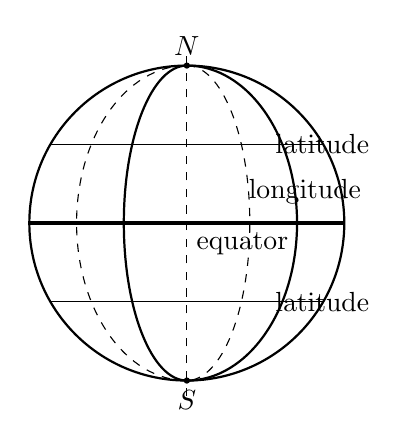
\begin{tikzpicture}[scale=2]
		% Sphere (side view -> circle)
		\draw[thick] (0,0) circle (1);
		
		% Axis (north--south)
		\draw[dashed] (0,-1.1) -- (0,1.1);
		\fill (0,1) circle (0.02) node[above] {$N$};
		\fill (0,-1) circle (0.02) node[below] {$S$};
		
		% Equator
		\draw[very thick] (-1,0) -- (1,0);
		\node[below right] at (0,0) {equator};
		
		% A few parallels (latitudes)
		\foreach \h/\labelpos in {0.5/right, -0.5/right}{
			% intersection with circle
			\pgfmathsetmacro{\x}{sqrt(1-\h*\h)}
			\draw (-\x,\h) -- (\x,\h);
		}
		\node[right] at (0.5,0.5) {latitude};
		\node[right] at (0.5,-0.5) {latitude};
		
		% A few meridians (longitudes) as ellipses
		% front meridians (solid)
		\draw[thick] (0,1) arc[start angle=90,end angle=270,
		x radius=0.4, y radius=1];
		\draw[thick] (0,1) arc[start angle=90,end angle=-90,
		x radius=0.7, y radius=1];
		
		% back meridians (dashed)
		\draw[dashed] (0,1) arc[start angle=90,end angle=270,
		x radius=0.7, y radius=1];
		\draw[dashed] (0,1) arc[start angle=90,end angle=-90,
		x radius=0.4, y radius=1];
		
		\node at (0.75,0.2) {longitude};
	\end{tikzpicture}
	\caption{Sphere with lines of longitude (meridians) and latitude (parallels).}
\end{figure}


	\begin{figure}[h]
		\centering
		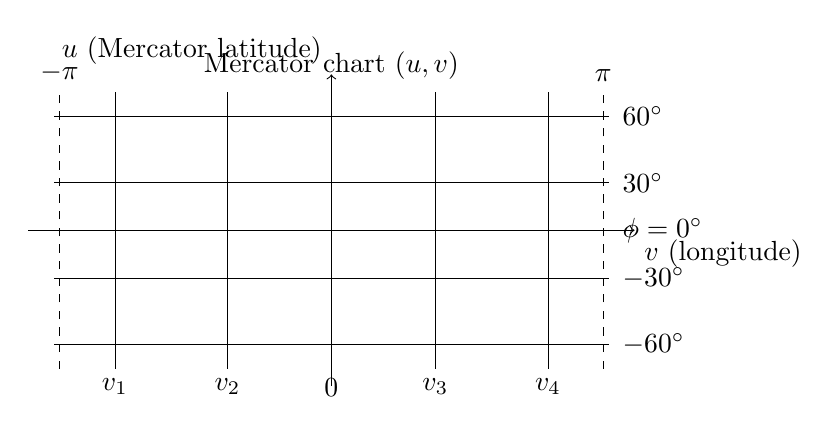
\begin{tikzpicture}[scale=1.1]
			% Axes
			\draw[->] (-3.5,0) -- (3.5,0) node[below right] {$v$ (longitude)};
			\draw[->] (0,-1.8) -- (0,1.8) node[above left] {$u$ (Mercator latitude)};
			
			% Domain boundary (approx -\pi < v < \pi)
			\draw[dashed] (-3.14,-1.6) -- (-3.14,1.6)
			node[above] {$-\pi$};
			\draw[dashed] ( 3.14,-1.6) -- ( 3.14,1.6)
			node[above] {$\pi$};
			
			% Vertical grid lines = longitudes v = const
			\foreach \x/\lab in {-2.5/{$v_1$}, -1.2/{$v_2$}, 0/{$0$}, 1.2/{$v_3$}, 2.5/{$v_4$}}{
				\draw[very thin] (\x,-1.6) -- (\x,1.6);
				\node[below] at (\x,-1.6) {\lab};
			}
			
			% Horizontal grid lines = latitudes u = const
			% approximate values: 0, \\ensuremath{\\pm}0.55 (\\ensuremath{\\approx}30\\textdegree{}), \\ensuremath{\\pm}1.32 (\\ensuremath{\\approx}60\\textdegree{})
			\foreach \y/\txt in {
				0/{$\phi=0^\circ$},
				0.55/{$30^\circ$},
				-0.55/{$-30^\circ$},
				1.32/{$60^\circ$},
				-1.32/{$-60^\circ$}
			}{
				\draw[very thin] (-3.2,\y) -- (3.2,\y);
				\node[right] at (3.25,\y) {\txt};
			}
			
			% Label
			\node at (0,1.9) {Mercator chart $(u,v)$};
		\end{tikzpicture}
		\caption{Mercator projection: longitudes and latitudes become straight lines
			in the $(u,v)$-plane. The spacing of latitudes increases with $|u|$, so areas
			near the poles are greatly magnified.}
	\end{figure}

\end{solution}

\subsection*{Main-text correspondence: VII/16}

\begin{problem}[CP-VII-0047 --- Problem 9. Gauss map: surjectivity, parity, and an elliptic point]
\label{prob:cp-vii-0047}
Let $S$ be a compact orientable surface in $\mathbb R^3$. Show that the Gauss map is surjective
	and that it hits almost every unit vector the same number of times modulo $2$.
	(You may use the Jordan--Brouwer separation theorem.) Show that $S$ always has an elliptic point.
	
	\par\medskip\noindent\textbf{Theory}\par\smallskip

	For an oriented surface $S\subset\mathbb R^3$, the \emph{Gauss map} is
	\[
	N:S\to S^2,\qquad p\mapsto N(p),
	\]
	where $N(p)$ is the unit normal at $p$.
	For $a\in S^2$, define the \emph{height function}
	\[
	h_a(p)=\langle p,a\rangle.
	\]
	Since $S$ is compact, $h_a$ attains a maximum and a minimum.
	At a critical point $p$ of $h_a$, the tangential component of $a$ vanishes, hence $a$ is normal
	to $S$ at $p$, i.e.\ $N(p)=\pm a$.
	
	By Sard's theorem, the set of regular values of $N$ has full measure in $S^2$; for a regular value
	$y$, the preimage $N^{-1}(y)$ is finite.
	For maps between compact $2$-manifolds, the parity $\#N^{-1}(y)\bmod 2$ is constant on the set
	of regular values (the mod-$2$ degree).
\end{problem}

\begin{solution}
\par\medskip\noindent\textbf{(1) Surjectivity.}\par\smallskip

	Fix $a\in S^2$. The function $h_a(p)=\langle p,a\rangle$ attains a maximum at some $p_{\max}\in S$
	and a minimum at some $p_{\min}\in S$.
	At each extremum, $a$ is normal to $S$, hence
	\[
	N(p_{\max})=\pm a,\qquad N(p_{\min})=\mp a.
	\]
	Thus $a$ lies in the image of $N$, and since $a$ was arbitrary, $N$ is surjective.
	
	\par\medskip\noindent\textbf{(2) Parity of the number of preimages.}\par\smallskip

	Let $y_0,y_1\in S^2$ be regular values of $N$. Choose a smooth path $\gamma:[0,1]\to S^2$
	from $y_0$ to $y_1$ avoiding the critical values of $N$.
	Then $M:=N^{-1}(\gamma([0,1]))$ is a compact $1$-manifold with boundary
	\[
	\partial M = N^{-1}(y_0)\,\cup\,N^{-1}(y_1).
	\]
	A compact $1$-manifold has an even number of boundary points, hence
	\[
	\#N^{-1}(y_0)\equiv \#N^{-1}(y_1)\pmod 2.
	\]
	Therefore, for almost every $y\in S^2$ (namely for every regular value) the number $\#N^{-1}(y)$
	is constant modulo $2$.
	
	\par\medskip\noindent\textbf{(3) Existence of an elliptic point.}\par\smallskip

	Choose $a\in S^2$ to be a regular value of $N$ (possible since regular values have full measure).
	Let $p$ be a maximum point of $h_a$ on $S$. Then $N(p)=\pm a$.
	Since $a$ is a regular value, $dN_p$ is invertible, so $\det(dN_p)\neq 0$.
	At a (nondegenerate) maximum the second fundamental form is definite, hence the principal curvatures
	have the same sign and are nonzero. Consequently $K(p)>0$, i.e.\ $p$ is an elliptic point.
	
	\par\medskip\noindent\textbf{Examples and intuition}\par\smallskip

	\begin{itemize}
		\item On a sphere, $N$ is (up to orientation) a diffeomorphism, so every direction is hit exactly once.
		\item On a torus in $\mathbb R^3$, most directions are hit several times; nevertheless the parity
		$\#N^{-1}(y)\bmod 2$ is constant for regular values $y$.
		\item Elliptic points occur at strictly convex supporting points (e.g.\ the ``outermost'' points
		for a generic height direction).
	\end{itemize}
	
	
	% Problem 9 diagram: height function + supporting planes
	
	\begin{figure}[htbp]
		\centering
		\begin{tikzpicture}[scale=1.15, line cap=round, line join=round, >=Latex]
			
			% --- Colors ---
			\definecolor{SurfBlue}{RGB}{40,110,180}
			\definecolor{DirRed}{RGB}{200,60,60}
			\definecolor{PlaneGray}{RGB}{120,120,120}
			\definecolor{ProjGreen}{RGB}{40,150,90}
			
			% Label box (opaque)
			\tikzset{lbl/.style={fill=white, fill opacity=1, text opacity=1, inner sep=2pt, rounded corners=1.2pt}}
			
			% --- Direction a (unit vector) ---
			% We'll use a direction roughly up-right
			\coordinate (O) at (0,0);
			\coordinate (aend) at (3.4,1.9);
			
			% --- A closed "surface cross-section" curve (schematic) ---
			% Think of it as the intersection of S with a plane containing a.
			\draw[very thick, SurfBlue]
			(0,0) .. controls (1.6,1.4) and (3.4,1.1) .. (4.3,0.1)
			.. controls (5.2,-1.0) and (4.0,-2.3) .. (2.1,-2.0)
			.. controls (0.4,-1.8) and (-0.6,-0.9) .. (0,0);
			
			% --- Height direction arrow a ---
			\draw[->, ultra thick, DirRed] (O) -- (aend);
			\node[lbl] at (3.65,2.15) {$a$};
			
			% --- Orthogonal direction to a (for drawing supporting lines) ---
			% We'll pick two support points and draw lines perpendicular to a through them.
			% Choose approximate points on the curve:
			\coordinate (pmax) at (3.9,0.9);
			\coordinate (pmin) at (1.2,-1.65);
			
			\fill (pmax) circle (1.4pt);
			\fill (pmin) circle (1.4pt);
			
			\node[lbl] at (4.55,1.15) {$p_{\max}$};
			\node[lbl] at (0.55,-1.95) {$p_{\min}$};
			
			% Supporting lines: perpendicular to a (schematic).
			% Vector perpendicular to aend-O is (-y, x): here use (-1.9,3.4) scaled.
			\coordinate (n1) at (-1.9,3.4);
			
			% Line through pmax: pmax + t*n1
			\draw[very thick, PlaneGray]
			($(pmax)+(-3,5.37)$) -- ($(pmax)+(3,-5.37)$);
			\node[lbl, text=PlaneGray] at ($(pmax)+(2.9,-0.25)$) {supporting plane};
			
			% Line through pmin
			\draw[very thick, PlaneGray]
			($(pmin)+(-3,5.37)$) -- ($(pmin)+(3,-5.37)$);
			\node[lbl, text=PlaneGray] at ($(pmin)+(2.9,-0.25)$) {supporting plane};
			
			% --- Normals at extrema align with \\ensuremath{\\pm}a ---
			\draw[->, very thick, DirRed] (pmax) -- ($(pmax)+(0.95,0.53)$);
			\node[lbl] at ($(pmax)+(1.25,0.85)$) {$N(p_{\max})=\pm a$};
			
			\draw[->, very thick, DirRed] (pmin) -- ($(pmin)+(-0.95,-0.53)$);
			\node[lbl] at ($(pmin)+(-1.35,-0.75)$) {$N(p_{\min})=\mp a$};
			
			% --- Height function annotation ---
			% Projection of points onto direction a (schematic)
			\draw[->, very thick, ProjGreen] (0.4,0.2) -- (1.25,0.68);
			\node[lbl, text=ProjGreen!60!black] at (1.65,0.88) {$h_a(p)=\langle p,a\rangle$};
			
			\node[lbl] at (2.6,-2.55) {\small maxima/minima of $h_a$ give normals parallel to $\pm a$};
			
		\end{tikzpicture}
		\caption{Problem 9: For a fixed direction $a\in S^2$, the height function $h_a(p)=\langle p,a\rangle$ attains a maximum and minimum on compact $S$. At such supporting points the tangent plane is orthogonal to $a$, hence $N(p)=\pm a$. This gives surjectivity of the Gauss map.}
	\end{figure}
	
	% Preamble:
	% \usepackage{tikz}
	% \usepackage{tikz-3dplot}
	% \usetikzlibrary{calc}
	
	
	% Problem 9 diagram (3D-looking): shaded surface + supporting planes
	
	\begin{figure}[htbp]
		\centering
		
		% viewing angle
		
		\begin{tikzpicture}[scale=1.15, line cap=round, line join=round, >=Latex]
			
			% --- Colors ---
			\definecolor{SurfBlue}{RGB}{40,110,180}
			\definecolor{PlanePurple}{RGB}{140,80,200}
			\definecolor{DirRed}{RGB}{200,60,60}
			\definecolor{PlaneGray}{RGB}{120,120,120}
			
			% Opaque label boxes
			\tikzset{
				lbl/.style={fill=white, fill opacity=1, text opacity=1, inner sep=2pt, rounded corners=1.2pt},
			}
			
			% --- Direction a: take a = e_z for a clean "height" picture ---
			\coordinate (O) at (0,0,0);
			\draw[->, ultra thick, DirRed] (O) -- (0,0,2.8);
			\node[lbl] at (0,0,3.05) {$a$};
			
			% --- A shaded "surface patch" (schematic compact surface piece) ---
			% (just a blob-like patch with a bit of waviness)
			\coordinate (S1) at (-2.4,-1.3, 0.25);
			\coordinate (S2) at (-2.0, 0.9, 0.80);
			\coordinate (S3) at (-0.6, 2.1, 1.10);
			\coordinate (S4) at ( 1.2, 1.7, 0.85);
			\coordinate (S5) at ( 2.5, 0.2, 0.45);
			\coordinate (S6) at ( 2.0,-1.7, 0.15);
			\coordinate (S7) at ( 0.2,-2.5, 0.55);
			\coordinate (S8) at (-1.7,-2.2, 0.35);
			
			% fill first (so edges/lines are visible)
			\fill[SurfBlue!12]
			(S1) .. controls (-2.6,-0.3,0.55) and (-2.0,0.6,0.95) .. (S2)
			.. controls (-1.3,1.6,1.20) and (-0.9,2.2,1.15) .. (S3)
			.. controls (0.4,2.4,1.00) and (1.1,2.0,0.95) .. (S4)
			.. controls (2.1,1.2,0.70) and (2.6,0.8,0.55) .. (S5)
			.. controls (2.8,-0.6,0.35) and (2.4,-1.4,0.25) .. (S6)
			.. controls (1.3,-2.4,0.05) and (0.7,-2.7,0.45) .. (S7)
			.. controls (-0.7,-2.7,0.75) and (-1.2,-2.5,0.45) .. (S8)
			.. controls (-2.2,-2.0,0.25) and (-2.5,-1.8,0.25) .. (S1);
			
			% outline
			\draw[very thick, SurfBlue]
			(S1) .. controls (-2.6,-0.3,0.55) and (-2.0,0.6,0.95) .. (S2)
			.. controls (-1.3,1.6,1.20) and (-0.9,2.2,1.15) .. (S3)
			.. controls (0.4,2.4,1.00) and (1.1,2.0,0.95) .. (S4)
			.. controls (2.1,1.2,0.70) and (2.6,0.8,0.55) .. (S5)
			.. controls (2.8,-0.6,0.35) and (2.4,-1.4,0.25) .. (S6)
			.. controls (1.3,-2.4,0.05) and (0.7,-2.7,0.45) .. (S7)
			.. controls (-0.7,-2.7,0.75) and (-1.2,-2.5,0.45) .. (S8)
			.. controls (-2.2,-2.0,0.25) and (-2.5,-1.8,0.25) .. (S1);
			
			% a couple of "contour" strokes to suggest 3D curvature
			\draw[thick, SurfBlue!70!black]
			(-2.1,-0.6,0.55) .. controls (-1.2,0.3,0.95) and (0.6,0.8,0.85) .. (2.0,0.2,0.55);
			\draw[thick, SurfBlue!70!black]
			(-1.6,-1.7,0.35) .. controls (-0.6,-1.1,0.65) and (0.8,-0.7,0.55) .. (1.8,-1.6,0.25);
			
			% --- Mark p_max and p_min (schematic) ---
			\coordinate (pmax) at (-0.2,0.4,1.55);
			\coordinate (pmin) at ( 0.8,-0.9,-0.65);
			
			\fill (pmax) circle (1.6pt);
			\fill (pmin) circle (1.6pt);
			
			\node[lbl] at ($ (pmax) + (0.7,0.25,0.25) $) {$p_{\max}$};
			\node[lbl] at ($ (pmin) + (0.9,-0.2,0.15) $) {$p_{\min}$};
			
			% --- Supporting planes for height direction a=e_z : z = const ---
			% Top supporting plane z = z_max
			\begin{scope}
				\fill[PlanePurple!14, opacity=0.35]
				(-3.0,-2.5,1.55) -- (3.0,-2.5,1.55) -- (3.0,2.5,1.55) -- (-3.0,2.5,1.55) -- cycle;
				\draw[very thick, dashed, PlanePurple]
				(-3.0,-2.5,1.55) -- (3.0,-2.5,1.55) -- (3.0,2.5,1.55) -- (-3.0,2.5,1.55) -- cycle;
				\node[lbl, text=PlanePurple!90!black] at (2.1,2.1,1.55) {\small supporting plane};
			\end{scope}
			
			% Bottom supporting plane z = z_min
			\begin{scope}
				\fill[PlanePurple!14, opacity=0.35]
				(-3.0,-2.5,-0.65) -- (3.0,-2.5,-0.65) -- (3.0,2.5,-0.65) -- (-3.0,2.5,-0.65) -- cycle;
				\draw[very thick, dashed, PlanePurple]
				(-3.0,-2.5,-0.65) -- (3.0,-2.5,-0.65) -- (3.0,2.5,-0.65) -- (-3.0,2.5,-0.65) -- cycle;
				\node[lbl, text=PlanePurple!90!black] at (2.1,2.1,-0.65) {\small supporting plane};
			\end{scope}
			
			% --- Normals at extrema align with \\ensuremath{\\pm}a (schematic arrows) ---
			\draw[->, very thick, DirRed] (pmax) -- ($ (pmax) + (0,0,0.8) $);
			\node[lbl] at ($ (pmax) + (0.9,0.1,0.85) $) {$N(p_{\max})=a$};
			
			\draw[->, very thick, DirRed] (pmin) -- ($ (pmin) + (0,0,-0.8) $);
			\node[lbl] at ($ (pmin) + (1.0,0.0,-0.85) $) {$N(p_{\min})=-a$};
			
			% --- Height function label ---
			\node[lbl, text=PlaneGray] at (-2.8,2.6,0.4) {\small $h_a(p)=\langle p,a\rangle$};
			
		\end{tikzpicture}
		
		\caption{Problem 9 (3D schematic): for a fixed direction $a$ (drawn as $e_z$), the height function
			$h_a(p)=\langle p,a\rangle$ has maxima/minima on compact $S$. The supporting planes $z=\text{const}$
			touch $S$ at $p_{\max},p_{\min}$, where the normals align with $\pm a$.}
	\end{figure}
	

	
	
	% Problem 10
\end{solution}

\subsection*{Main-text correspondence: VII/17}

\begin{problem}[CP-VII-0048 --- Problem 12 --- Gauss curvature via the map $fN$; curvature of an ellipsoid]
\label{prob:cp-vii-0048}
Let $S\subset\mathbb R^3$ be an oriented smooth surface with Gauss map (unit normal) $N$.
	Let $V\subset S$ be open and let $f:V\to\mathbb R$ be smooth and nowhere zero.
	Let $v_1,v_2$ be smooth tangent vector fields on $V$ such that at each point they are orthonormal and oriented,
	i.e.\ $v_1\wedge v_2=N$ (equivalently $v_1\times v_2=N$).
	
	\begin{enumerate}
		\item Prove that the Gaussian curvature $K$ on $V$ is
		\[
		K \;=\; \frac{\big\langle D(fN)(v_1)\wedge D(fN)(v_2),\, fN\big\rangle}{f^3}.
		\]
		\item Let $f$ be the restriction to the ellipsoid
		\[
		E:\qquad \frac{x^2}{a^2}+\frac{y^2}{b^2}+\frac{z^2}{c^2}=1
		\]
		of the function
		\[
		f(x,y,z)=\sqrt{\frac{x^2}{a^4}+\frac{y^2}{b^4}+\frac{z^2}{c^4}}.
		\]
		Show that the Gaussian curvature of $E$ is
		\[
		K=\frac{1}{a^2b^2c^2\, f^4}.
		\]
	\end{enumerate}
	
	\medskip
	\textbf{Theory.}
	For an oriented orthonormal basis $(v_1,v_2)$ of $T_pS$,
	\[
	K(p)=\det(S_p)=\big\langle dN_p(v_1)\times dN_p(v_2),\,N(p)\big\rangle,
	\]
	because $S=-dN$ and $\det(-S)=\det(S)$. Also $\langle N\times X,\,N\rangle=0$ for all $X$.
	
	\medskip
\end{problem}

\begin{solution}
\textbf{(i)} Set $F=fN:V\to\mathbb R^3$. For any $v\in T_pS$,
	\[
	dF_p(v)=v(f)\,N(p)+f(p)\,dN_p(v).
	\]
	Hence
	\[
	dF(v_1)\times dF(v_2)
	=
	\big(v_1(f)N+f\,dN(v_1)\big)\times\big(v_2(f)N+f\,dN(v_2)\big)
	\]
	\[
	= f^2\,dN(v_1)\times dN(v_2)
	+ f\,v_1(f)\,N\times dN(v_2)
	+ f\,v_2(f)\,dN(v_1)\times N.
	\]
	Taking the dot product with $fN$ kills the mixed terms since
	$\langle N\times dN(v_2),N\rangle=0$ and $\langle dN(v_1)\times N,N\rangle=0$.
	Thus
	\[
	\big\langle dF(v_1)\times dF(v_2),\,fN\big\rangle
	=
	f^3\,\big\langle dN(v_1)\times dN(v_2),\,N\big\rangle.
	\]
	But for an oriented orthonormal pair $(v_1,v_2)$, the Gauss curvature is
	\[
	K=\big\langle dN(v_1)\times dN(v_2),\,N\big\rangle.
	\]
	Therefore
	\[
	K=\frac{\big\langle dF(v_1)\times dF(v_2),\,fN\big\rangle}{f^3}
	=
	\frac{\big\langle D(fN)(v_1)\wedge D(fN)(v_2),\,fN\big\rangle}{f^3}.
	\]
	
	\medskip
	\textbf{(ii)} Let $\Phi(x,y,z)=\frac{x^2}{a^2}+\frac{y^2}{b^2}+\frac{z^2}{c^2}$, so $E=\{\Phi=1\}$ and
	\[
	\nabla\Phi=\left(\frac{2x}{a^2},\frac{2y}{b^2},\frac{2z}{c^2}\right),\qquad
	\|\nabla\Phi\|=2\sqrt{\frac{x^2}{a^4}+\frac{y^2}{b^4}+\frac{z^2}{c^4}}=2f.
	\]
	Hence the unit normal is
	\[
	N=\frac{\nabla\Phi}{\|\nabla\Phi\|}=\frac1f\left(\frac{x}{a^2},\frac{y}{b^2},\frac{z}{c^2}\right),
	\quad\text{so}\quad
	fN=\left(\frac{x}{a^2},\frac{y}{b^2},\frac{z}{c^2}\right).
	\]
	Write $A=\mathrm{diag}\!\left(\frac1{a^2},\frac1{b^2},\frac1{c^2}\right)$. Then $fN=Ax$ and thus
	\[
	D(fN)(v)=Av.
	\]
	Applying (i),
	\[
	K=\frac{\langle (Av_1)\times(Av_2),\,fN\rangle}{f^3}.
	\]
	Use the identity $(Au)\times(Av)=\det(A)\,A^{-T}(u\times v)$. Since $A$ is diagonal, $A^{-T}=A^{-1}$, and
	$v_1\times v_2=N$, we obtain
	\[
	(Av_1)\times(Av_2)=\det(A)\,A^{-1}N.
	\]
	Therefore
	\[
	\langle (Av_1)\times(Av_2),\,fN\rangle
	=\det(A)\,\langle A^{-1}N,\,fN\rangle.
	\]
	But $N=\frac1f Ax$, hence $A^{-1}N=\frac1f x$, and $fN=Ax$, so
	\[
	\langle A^{-1}N,\,fN\rangle
	=\left\langle \frac1f x,\,Ax\right\rangle
	=\frac1f\left(\frac{x^2}{a^2}+\frac{y^2}{b^2}+\frac{z^2}{c^2}\right)
	=\frac1f
	\]
	on $E$. Also $\det(A)=\frac1{a^2b^2c^2}$. Hence
	\[
	\langle (Av_1)\times(Av_2),\,fN\rangle=\frac{1}{a^2b^2c^2\,f},
	\qquad
	K=\frac{1}{a^2b^2c^2\,f^4}.
	\]
	
	\medskip
	\textbf{Example (sphere check).}
	If $a=b=c=R$, then $f=1/R$ on $E$, so $K=\frac{1}{R^6(1/R^4)}=\frac1{R^2}$.
\end{solution}

\begin{problem}[CP-VII-0049 --- Problem 7. Mean curvature as an average of normal curvatures]
\label{prob:cp-vii-0049}
Show that the mean curvature $H$ at $p\in S$ is given by
\[
H=\frac1\pi\int_0^\pi k_n(\theta)\,d\theta,
\]
where $k_n(\theta)$ is the normal curvature at $p$ along a direction making an angle $\theta$ with a fixed direction.

\medskip
\end{problem}

\begin{solution}
Let $k_1,k_2$ be the principal curvatures at $p$, with orthonormal principal directions
$e_1,e_2\in T_pS$.
Any unit tangent direction making angle $\theta$ with $e_1$ is
\[
t(\theta)=\cos\theta\,e_1+\sin\theta\,e_2.
\]
By Euler's formula for normal curvature,
\[
k_n(\theta)=k_1\cos^2\theta+k_2\sin^2\theta.
\]
Hence
\[
\frac1\pi\int_0^\pi k_n(\theta)\,d\theta
=\frac1\pi\int_0^\pi\bigl(k_1\cos^2\theta+k_2\sin^2\theta\bigr)\,d\theta
=\frac1\pi\left(k_1\cdot\frac\pi2+k_2\cdot\frac\pi2\right)
=\frac{k_1+k_2}{2}.
\]
But $H=\dfrac{k_1+k_2}{2}$, so
\[
H=\frac1\pi\int_0^\pi k_n(\theta)\,d\theta.
\]
(Using $[0,\pi]$ is natural since $k_n(\theta)$ has period $\pi$.)

\bigskip

\begin{figure}[htbp]
	\centering
	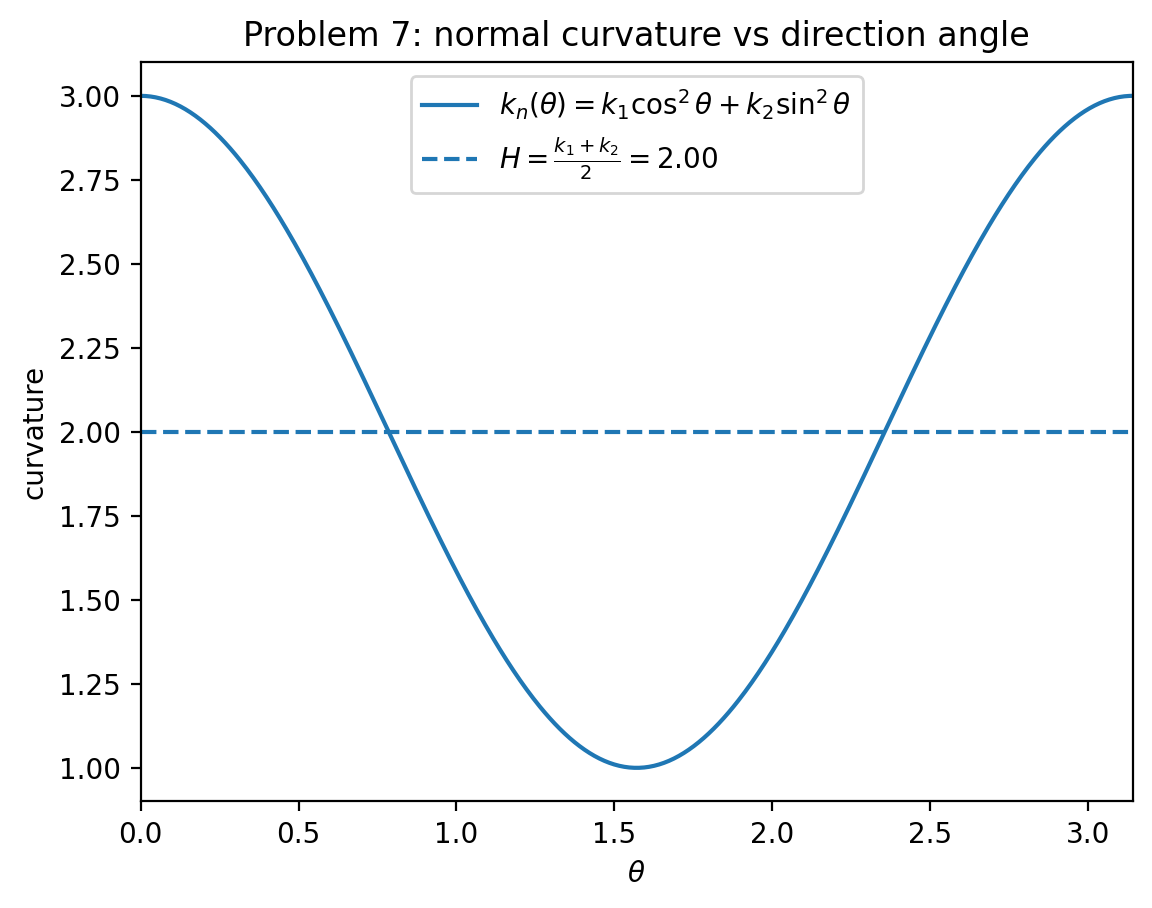
\includegraphics[width=0.72\linewidth]{chapters/part07_volume_vii/figures/problem7_kn_vs_theta.png}
	\caption{Problem 7: Normal curvature $k_n(\theta)$ versus direction angle $\theta$, with the mean curvature line $H$.}
\end{figure}





\par\medskip\noindent\textbf{Theory: normal curvature, principal curvatures, and mean curvature}\par\smallskip


Let $S\subset\mathbb R^3$ be a smooth surface and $p\in S$. Fix a unit normal $N$ near $p$.
For a unit tangent direction $t\in T_pS$ ($\|t\|=1$), the \emph{normal curvature} $k_n(t)$
is the (signed) curvature at $p$ of the normal section curve obtained by intersecting $S$
with the plane spanned by $t$ and $N(p)$.

Equivalently, using the shape operator (Weingarten map)
\[
S_p:T_pS\to T_pS,\qquad S_p(v)=-dN_p(v),
\]
the second fundamental form is
\[
\mathrm{II}(u,v)=\langle S_p(u),v\rangle,
\]
and for unit $t$ one has
\[
k_n(t)=\mathrm{II}(t,t)=\langle S_p(t),t\rangle.
\]

Since $S_p$ is self-adjoint on the $2$-dimensional inner-product space $T_pS$, there is an
orthonormal basis of eigenvectors $e_1,e_2$ such that
\[
S_p(e_1)=k_1 e_1,\qquad S_p(e_2)=k_2 e_2,
\]
where $k_1,k_2$ are the \emph{principal curvatures} and $e_1,e_2$ are the corresponding
\emph{principal directions}. Writing any unit direction as
\[
t(\theta)=\cos\theta\,e_1+\sin\theta\,e_2,
\]
Euler's formula for normal curvature gives
\[
k_n(\theta)=k_1\cos^2\theta+k_2\sin^2\theta.
\]
The \emph{mean curvature} is defined by
\[
H=\frac{k_1+k_2}{2}.
\]
Using $\int_0^\pi \cos^2\theta\,d\theta=\int_0^\pi \sin^2\theta\,d\theta=\frac{\pi}{2}$,
one obtains
\[
\frac1\pi\int_0^\pi k_n(\theta)\,d\theta
=\frac1\pi\int_0^\pi\bigl(k_1\cos^2\theta+k_2\sin^2\theta\bigr)\,d\theta
=\frac{k_1+k_2}{2}=H.
\]
(Integrating over $[0,\pi]$ is natural since $k_n(\theta)$ has period $\pi$.)


% Theory diagram (TikZ) --- larger + colored


% Theory diagram (TikZ) --- labels not occluded

% in preamble (once):
% \usetikzlibrary{calc}
% (optional) \usetikzlibrary{backgrounds}


% Theory diagram (TikZ) --- labels ALWAYS on top + opaque boxes

\begin{figure}[htbp]
	\centering
	\begin{tikzpicture}[scale=1.45, line cap=round, line join=round, >=Latex]
		
		% --- Layers (geometry below, labels above) ---
		\pgfdeclarelayer{bg}
		\pgfdeclarelayer{fg}
		\pgfsetlayers{bg,main,fg}
		
		% --- Colors ---
		\definecolor{SurfBlue}{RGB}{40,110,180}
		\definecolor{PlaneGray}{RGB}{120,120,120}
		\definecolor{NormalRed}{RGB}{200,60,60}
		\definecolor{TangGreen}{RGB}{40,150,90}
		\definecolor{SectionPurple}{RGB}{140,80,200}
		\definecolor{CurveOrange}{RGB}{220,130,30}
		
		% --- OPAQUE label style (this is the key) ---
		\tikzset{
			lbl/.style={
				fill=white,              % fully opaque white
				fill opacity=1,          % DO NOT make this < 1
				text opacity=1,
				inner sep=2.2pt,
				rounded corners=1.4pt,
				draw=none
			},
			lead/.style={->, very thin, black!60} % leader line
		}
		
		% --- Point p ---
		\coordinate (P) at (0,0);
		
		% --- Tangent plane at p (parallelogram) ---
		\coordinate (A) at (-2.2,-0.5);
		\coordinate (B) at ( 2.2,-0.5);
		\coordinate (C) at ( 2.6, 0.5);
		\coordinate (D) at (-1.8, 0.5);
		
		% --- Normal section plane (tilted strip) ---
		\coordinate (E) at (0.5,-1.2);
		\coordinate (F) at (2.7,-0.2);
		\coordinate (G) at (2.2, 2.25);
		\coordinate (H) at (0.0, 1.25);
		
		
		% Background fills
		
		\begin{pgfonlayer}{bg}
			\fill[PlaneGray!12] (A) -- (B) -- (C) -- (D) -- cycle;
			\fill[SectionPurple!10] (E) -- (F) -- (G) -- (H) -- cycle;
		\end{pgfonlayer}
		
		
		% Geometry (main layer)
		
		
		% surface patch
		\draw[very thick, SurfBlue] (-3,-0.8) .. controls (-1,-0.2) and (1,-0.2) .. (3,-0.8);
		\draw[very thick, SurfBlue] (-3, 0.8) .. controls (-1, 0.2) and (1, 0.2) .. (3, 0.8);
		\draw[very thick, SurfBlue] (-3,-0.8) .. controls (-2,0) and (-1,0) .. (-3,0.8);
		\draw[very thick, SurfBlue] ( 3,-0.8) .. controls ( 2,0) and ( 1,0) .. ( 3,0.8);
		
		% tangent plane border
		\draw[very thick, PlaneGray] (A) -- (B) -- (C) -- (D) -- cycle;
		
		% normal-section plane border
		\draw[very thick, dashed, SectionPurple] (E) -- (F) -- (G) -- (H) -- cycle;
		
		% point p
		\fill (P) circle (1.7pt);
		
		% normal vector N
		\draw[->, ultra thick, NormalRed] (P) -- (0,2.45);
		
		% tangent direction t(theta)
		\draw[->, ultra thick, TangGreen] (P) -- (2.25,0.75);
		
		% normal section curve
		\draw[ultra thick, CurveOrange]
		(0.15,-0.15) .. controls (1.0,0.32) and (1.65,0.98) .. (2.18,1.85);
		
		
		% Labels (foreground layer)
		
		\begin{pgfonlayer}{fg}
			
			% p
			\node[lbl, anchor=north east] at ($(P)+(-0.12,-0.12)$) {$p$};
			
			% TpS label (moved away)
\node[lbl, text=PlaneGray] (tps) at (3.85,1.05) {$T_pS$};
\draw[lead] (tps.west) -- ($(C)!0.65!(D)$);
			
			% N(p)
			\node[lbl] (Np) at (0,2.75) {$N(p)$};
			\draw[lead] (Np.south) -- (0,2.45);
			
			% t(theta)
			\node[lbl] (tt) at (2.95,1.15) {$t(\theta)$};
			\draw[lead] (tt.west) -- (2.25,0.75);
			
			% normal-section plane label OUTSIDE + leader (no overlap)
			\node[lbl, text=SectionPurple!90!black] (nsp) at (3.35,2.05) {\small normal-section plane};
			\draw[lead] (nsp.west) -- ($(G)!0.55!(H)$);
			
			% normal section label OUTSIDE + leader
			\node[lbl, text=CurveOrange!90!black] (ns) at (3.10,0.25) {\small normal section};
			\draw[lead] (ns.west) -- (1.55,0.70);
			
		\end{pgfonlayer}
		
	\end{tikzpicture}
	\caption{Normal curvature: the plane spanned by $t(\theta)\in T_pS$ and $N(p)$ cuts the surface in a normal section curve whose curvature at $p$ equals $k_n(\theta)$.}
\end{figure}



% Embed the two charts (Problem 7 + Problem 8)

\begin{figure}[htbp]
	\centering
	
	\begin{minipage}[t]{0.485\linewidth}
		\centering
		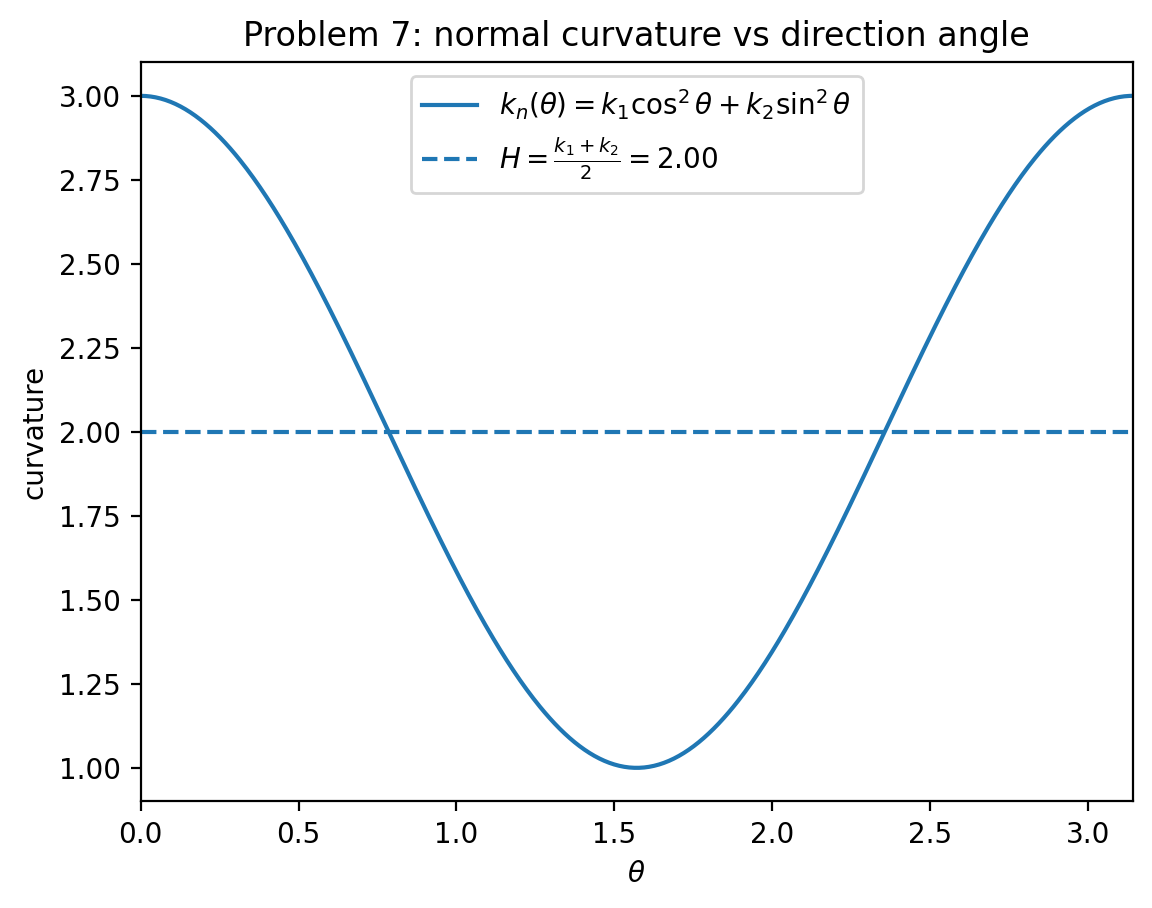
\includegraphics[width=\linewidth]{chapters/part07_volume_vii/figures/problem7_kn_vs_theta.png}
		\caption*{\small Problem 7: $k_n(\theta)$ vs. $\theta$ and the average line $H$.}
	\end{minipage}
	\hfill
	\begin{minipage}[t]{0.485\linewidth}
		\centering
		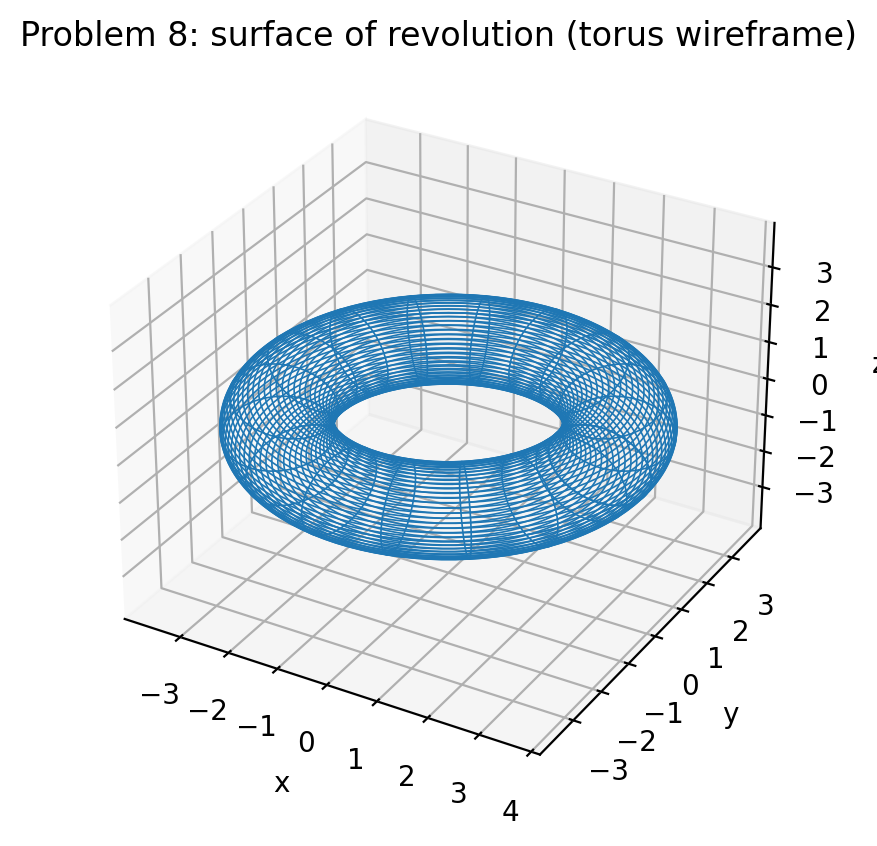
\includegraphics[width=\linewidth]{chapters/part07_volume_vii/figures/problem8_torus_wireframe.png}
		\caption*{\small Problem 8: example surface of revolution (torus wireframe).}
	\end{minipage}
	
	\caption{Charts accompanying Problems 7--8.}
\end{figure}

\par\medskip\noindent\textbf{Examples and interpretation (Problem 7)}\par\smallskip


\par\medskip\noindent\textbf{Example 1: principal directions minimize/maximize $k_n$}\par\smallskip

Let $k_1\le k_2$ be the principal curvatures at $p$, with principal directions $e_1,e_2$.
Euler's formula gives
\[
k_n(\theta)=k_1\cos^2\theta+k_2\sin^2\theta.
\]
Hence
\[
k_n(0)=k_1,\qquad k_n\Bigl(\frac{\pi}{2}\Bigr)=k_2,
\]
so the normal curvature is smallest along $e_1$ and largest along $e_2$.
Moreover,
\[
k_1\le k_n(\theta)\le k_2 \quad\text{for all }\theta,
\]
since $k_n(\theta)$ is a convex combination of $k_1$ and $k_2$.

\par\medskip\noindent\textbf{Example 2: the average over directions equals the mean curvature}\par\smallskip

Using Euler's formula and the identities
\[
\int_0^\pi \cos^2\theta\,d\theta=\int_0^\pi \sin^2\theta\,d\theta=\frac{\pi}{2},
\]
we obtain
\[
\frac{1}{\pi}\int_0^\pi k_n(\theta)\,d\theta
=\frac{1}{\pi}\int_0^\pi\bigl(k_1\cos^2\theta+k_2\sin^2\theta\bigr)\,d\theta
=\frac{k_1+k_2}{2}=H.
\]
Thus $H$ is literally the \emph{directional average} of the normal curvature at $p$.

\par\medskip\noindent\textbf{Example 3: elliptic / hyperbolic / parabolic points via $k_1,k_2$}\par\smallskip

The signs of $k_1$ and $k_2$ determine the local shape:
\begin{itemize}
	\item \textbf{Elliptic point:} $k_1k_2>0$ (both same sign). Then $k_n(\theta)$ keeps the same sign for all directions.
	\item \textbf{Hyperbolic point:} $k_1k_2<0$ (opposite signs). Then $k_n(\theta)$ changes sign as $\theta$ varies, so there are directions with $k_n(\theta)=0$ (asymptotic directions).
	\item \textbf{Parabolic point:} $k_1k_2=0$ (one principal curvature $0$). Then $k_n(\theta)$ vanishes in at least one principal direction.
\end{itemize}
In all cases, the mean curvature $H=(k_1+k_2)/2$ measures the ``average bending''.

\par\medskip\noindent\textbf{Example 4: quick check on a sphere and a cylinder}\par\smallskip

\begin{itemize}
	\item \textbf{Sphere of radius $R$:} $k_1=k_2=\frac{1}{R}$, so
	\[
	k_n(\theta)=\frac{1}{R}\quad\text{(independent of $\theta$)},\qquad
	H=\frac{1}{R}.
	\]
	The integral formula gives $\frac{1}{\pi}\int_0^\pi \frac{1}{R}\,d\theta=\frac{1}{R}$ as expected.
	
	\item \textbf{Cylinder of radius $R$:} principal curvatures are $k_1=0$ (along the axis direction) and $k_2=\frac{1}{R}$ (around the circular direction). Then
	\[
	k_n(\theta)=0\cdot\cos^2\theta+\frac{1}{R}\sin^2\theta=\frac{1}{R}\sin^2\theta,
	\qquad
	H=\frac{1}{2R}.
	\]
	Indeed,
	\[
	\frac{1}{\pi}\int_0^\pi \frac{1}{R}\sin^2\theta\,d\theta
	=\frac{1}{R}\cdot\frac{1}{\pi}\cdot\frac{\pi}{2}
	=\frac{1}{2R}=H.
	\]
\end{itemize}


\par\medskip\noindent\textbf{Principal directions (definition)}\par\smallskip

Let $S\subset\mathbb R^3$ be a smooth surface and $p\in S$. Fix a unit normal field $N$ near $p$
and consider the shape operator (Weingarten map)
\[
S_p:T_pS\to T_pS,\qquad S_p(v)=-dN_p(v).
\]
A nonzero tangent vector $v\in T_pS$ is called a \emph{principal direction} at $p$ if it is an
eigenvector of $S_p$, i.e.\ if there exists $\kappa\in\mathbb R$ such that
\[
S_p(v)=\kappa\,v.
\]
The corresponding eigenvalue $\kappa$ is the \emph{principal curvature} in that direction.

Equivalently, if $t$ is a unit tangent vector, then $t$ is a principal direction iff it is a
critical direction of the normal curvature function $t\mapsto k_n(t)$ on the unit circle in $T_pS$
(and the critical values are precisely the principal curvatures).
In a principal orthonormal basis $\{e_1,e_2\}$ one has
\[
S_p(e_1)=k_1e_1,\qquad S_p(e_2)=k_2e_2,
\]
and $\{e_1,e_2\}$ are the principal directions at $p$ (unique up to sign, and up to rotation if
$k_1=k_2$).
\end{solution}

\begin{problem}[CP-VII-0050 --- Problem 11. Gauss curvature as spherical area distortion]
\label{prob:cp-vii-0050}
Let $p$ be a point of a surface $S$ such that the Gaussian curvature $K(p)\neq 0$, and let $V$
	be a small connected neighbourhood of $p$ where $K$ does not change sign.
	Define the \emph{spherical area} $A_N(B)$ of a domain $B\subset V$ to be the area of $N(B)$ if
	$K(p)>0$, or minus the area of $N(B)$ if $K(p)<0$ (where $N$ is the Gauss map).
	Show that
	\[
	K(p)=\lim_{A(B)\to 0}\frac{A_N(B)}{A(B)},
	\]
	where $A(B)$ is the area of $B$ and the limit is taken through a sequence of domains $B_n$
	converging to $p$ (eventually contained in every ball around $p$).
	
	\par\medskip\noindent\textbf{Theory (area change under the Gauss map)}\par\smallskip

	For an oriented surface, the Gauss map $N:S\to S^2$ has differential $dN_p:T_pS\to T_{N(p)}S^2$.
	Its Jacobian determinant equals the Gaussian curvature:
	\[
	\det(dN_p)=K(p).
	\]
	If $N$ is a local diffeomorphism on a region $B$ and $K$ has constant sign on $B$, then the area
	formula for smooth maps between surfaces yields
	\[
	\operatorname{area}(N(B))=\int_B |\det(dN_q)|\,dA(q)=\int_B |K(q)|\,dA(q).
	\]
	The signed spherical area $A_N(B)$ is defined precisely so that the absolute value is removed when
	$K$ has constant sign.
\end{problem}

\begin{solution}
\textbf{Solution.}
	Since $K(p)\neq 0$ and $K$ is continuous, after shrinking $V$ we may assume $K(q)\neq 0$ on $V$,
	so $dN_q$ is invertible and hence $N$ is a local diffeomorphism on $V$.
	Let $B\subset V$ be a domain. By the area formula,
	\[
	\operatorname{area}(N(B))=\int_B |K(q)|\,dA(q).
	\]
	Because $K$ does not change sign on $V$, the definition of $A_N(B)$ gives
	\[
	A_N(B)=\int_B K(q)\,dA(q).
	\]
	Therefore
	\[
	\frac{A_N(B)}{A(B)}=\frac{1}{A(B)}\int_B K(q)\,dA(q),
	\]
	which is the average value of $K$ over $B$.
	Let $B_n\to p$ with $A(B_n)\to 0$. By continuity of $K$, the average value over $B_n$ tends to
	$K(p)$, i.e.
	\[
	\lim_{n\to\infty}\frac{1}{A(B_n)}\int_{B_n}K\,dA = K(p).
	\]
	Hence
	\[
	K(p)=\lim_{A(B)\to 0}\frac{A_N(B)}{A(B)}.
	\]
	
	\par\medskip\noindent\textbf{Examples and intuition}\par\smallskip

	\begin{itemize}
		\item \textbf{Sphere of radius $R$.} One has $K\equiv 1/R^2$ and small areas satisfy
		$\operatorname{area}(N(B))\sim (1/R^2)\operatorname{area}(B)$, so the ratio tends to $1/R^2$.
		\item \textbf{Plane.} The Gauss map is constant, so $\operatorname{area}(N(B))=0$ and the ratio
		is $0$, consistent with $K\equiv 0$.
		\item \textbf{Cylinder.} The Gauss map image is 1-dimensional (a circle), so spherical area is
		$0$ and the ratio is $0$, consistent with $K\equiv 0$.
	\end{itemize}
	
	% Preamble:
	% \usepackage{tikz}
	% \usepackage{tikz-3dplot}
	% \usetikzlibrary{calc}
	
	
	% Problem 11 diagram: patch B on S and its Gauss image N(B) on S^2
	
	\begin{figure}[htbp]
		\centering
		
		\begin{tikzpicture}[scale=1.10, line cap=round, line join=round, >=Latex]
			
			% --- Colors ---
			\definecolor{SurfBlue}{RGB}{40,110,180}
			\definecolor{PatchPurple}{RGB}{140,80,200}
			\definecolor{DirRed}{RGB}{200,60,60}
			\definecolor{Gray}{RGB}{110,110,110}
			
			% Opaque labels (prevents occlusion)
			\tikzset{
				lbl/.style={fill=white, fill opacity=1, text opacity=1, inner sep=2pt, rounded corners=1.2pt},
				arr/.style={->, very thick},
			}
			
			
			% LEFT: surface patch B \\ensuremath{\\subset} S
			
			\begin{scope}[shift={(-4.8,0,0)}]
				
				% A schematic curved surface patch boundary
				\coordinate (A) at (-1.8,-1.1, 0.25);
				\coordinate (B) at ( 1.6,-1.0, 0.10);
				\coordinate (C) at ( 1.9, 1.2, 0.55);
				\coordinate (D) at (-1.5, 1.1, 0.75);
				
				% Fill patch (curvy quadrilateral)
				\fill[SurfBlue!14]
				(A) .. controls (-0.8,-1.2,0.35) and (0.8,-1.2,0.15) .. (B)
				.. controls (2.2,-0.2,0.05) and (2.2,0.8,0.45) .. (C)
				.. controls (0.7,1.55,0.75) and (-0.5,1.5,0.85) .. (D)
				.. controls (-2.1,0.4,0.95) and (-2.2,-0.4,0.45) .. cycle;
				
				\draw[very thick, SurfBlue]
				(A) .. controls (-0.8,-1.2,0.35) and (0.8,-1.2,0.15) .. (B)
				.. controls (2.2,-0.2,0.05) and (2.2,0.8,0.45) .. (C)
				.. controls (0.7,1.55,0.75) and (-0.5,1.5,0.85) .. (D)
				.. controls (-2.1,0.4,0.95) and (-2.2,-0.4,0.45) .. cycle;
				
				% A few short normal arrows on the patch
				\foreach \px/\py/\pz in {-0.9/-0.2/0.55, 0.3/0.1/0.45, 1.1/0.4/0.50} {
					\coordinate (P) at (\px,\py,\pz);
					\draw[arr, DirRed] (P) -- ++(0.0,0.0,0.85);
				}
				
				% Labels
				\node[lbl] at (0.0,1.55,1.10) {$S$};
				\node[lbl] at (-0.2,0.0,0.95) {$B$};
				\node[lbl, text=Gray] at (0.6,-1.65,0.05) {\small area $A(B)$};
				
			\end{scope}
			
			
			% MIDDLE: arrow representing Gauss map N
			
			\draw[arr, Gray] (-1.6,0,0.7) -- (1.6,0,0.7);
			\node[lbl, text=Gray] at (0,0.25,0.9) {Gauss map $N$};
			
			
			% RIGHT: sphere S^2 with patch N(B)
			
			\begin{scope}[shift={(4.8,0,0)}]
				
				% Draw a unit sphere (schematic): a circle + "equator" ellipse to suggest 3D
				% Sphere centered at (0,0,0)
				\draw[very thick] (0,0,0) circle (2.0); % outer silhouette in this projection
				
				% An "equator" ellipse (visual cue)
				\draw[thick, dashed] (0,0,0) ellipse (2.0 and 0.75);
				
				% A small spherical patch near the "upper right" of the sphere
				\coordinate (P1) at (0.7,1.3,1.1);
				\coordinate (P2) at (1.4,1.0,0.8);
				\coordinate (P3) at (1.2,1.6,0.9);
				\coordinate (P4) at (0.9,1.7,1.2);
				
				\fill[PatchPurple!18, opacity=0.55]
				(P1) .. controls (1.0,1.25,1.0) and (1.25,1.05,0.85) .. (P2)
				.. controls (1.55,1.25,0.75) and (1.45,1.45,0.85) .. (P3)
				.. controls (1.15,1.85,0.95) and (1.0,1.85,1.15) .. (P4)
				.. controls (0.75,1.65,1.25) and (0.65,1.45,1.20) .. cycle;
				
				\draw[very thick, PatchPurple]
				(P1) .. controls (1.0,1.25,1.0) and (1.25,1.05,0.85) .. (P2)
				.. controls (1.55,1.25,0.75) and (1.45,1.45,0.85) .. (P3)
				.. controls (1.15,1.85,0.95) and (1.0,1.85,1.15) .. (P4)
				.. controls (0.75,1.65,1.25) and (0.65,1.45,1.20) .. cycle;
				
				% Labels
				\node[lbl] at (0.0,2.45,0.0) {$S^2$};
				\node[lbl] at (1.35,1.85,1.25) {$N(B)$};
				\node[lbl, text=Gray] at (0.0,-2.65,0.0) {\small signed area $A_N(B)$};
				
			\end{scope}
			
			
			% Bottom caption-like formula (inside figure)
			
			\node[lbl, text=Gray] at (0,-3.05,0.0)
			{\small $K(p)=\displaystyle\lim_{A(B)\to 0}\frac{A_N(B)}{A(B)}$};
			
		\end{tikzpicture}
		
		\caption{Problem 11: a small patch $B\subset S$ is mapped by the Gauss map $N$ to a patch $N(B)\subset S^2$.
			The Gaussian curvature at $p$ is the infinitesimal ratio of signed spherical area to surface area.}
	\end{figure}
	
	\par\medskip\noindent\textbf{Why one may view $dN_p$ as a map $T_pS\to T_pS$}\par\smallskip

	
	Formally, the Gauss map is
	\[
	N:S\to S^2,\qquad p\mapsto N(p),
	\]
	so its differential at $p$ is a linear map
	\[
	dN_p:T_pS\longrightarrow T_{N(p)}S^2.
	\]
	At first glance the domain and codomain are different tangent planes. However, for the Gauss map
	there is a canonical identification of these two planes inside $\mathbb R^3$.
	
	\par\medskip\noindent\textbf{Step 1: $dN_p(v)$ is tangent to the sphere.}\par\smallskip

	Since $\|N\|^2=\langle N,N\rangle=1$ on $S$, differentiating at $p$ in the direction $v\in T_pS$
	gives
	\[
	0=d(\langle N,N\rangle)_p(v)=2\langle dN_p(v),N(p)\rangle.
	\]
	Hence
	\[
	\langle dN_p(v),N(p)\rangle=0,
	\]
	so $dN_p(v)$ is orthogonal to $N(p)$, i.e.
	\[
	dN_p(v)\in T_{N(p)}S^2=\{w\in\mathbb R^3:\langle w,N(p)\rangle=0\}.
	\]
	
	\par\medskip\noindent\textbf{Step 2: $T_pS$ and $T_{N(p)}S^2$ are the same $2$-plane in $\mathbb R^3$.}\par\smallskip

	Because $N(p)$ is also the unit normal to $S$ at $p$, the tangent plane to $S$ at $p$ is
	\[
	T_pS=\{w\in\mathbb R^3:\langle w,N(p)\rangle=0\}.
	\]
	But this is exactly the same description as the tangent plane to the unit sphere at $N(p)$:
	\[
	T_{N(p)}S^2=\{w\in\mathbb R^3:\langle w,N(p)\rangle=0\}.
	\]
	Therefore, as subspaces of $\mathbb R^3$,
	\[
	T_pS = T_{N(p)}S^2.
	\]
	With this identification, we may regard
	\[
	dN_p:T_pS\to T_pS.
	\]
	
	\par\medskip\noindent\textbf{Step 3: The shape operator.}\par\smallskip

	Using the above identification, one defines the \emph{shape operator} (Weingarten map) by
	\[
	S_p:=-\,dN_p:T_pS\to T_pS.
	\]
	Its eigenvectors are the \emph{principal directions}, its eigenvalues are the \emph{principal curvatures},
	and one has
	\[
	K(p)=\det(S_p),\qquad 2H(p)=\operatorname{tr}(S_p),
	\]
	with the sign of $H$ depending on the chosen orientation of $N$, while $K$ does not.
	
	\par\medskip\noindent\textbf{Geometric analogy (circle) and what the Gauss map does}\par\smallskip

	
	It is helpful to first look at the $1$-dimensional analogue.
	Let $\gamma:I\to\mathbb R^2$ be a unit-speed plane curve, with unit tangent $T(s)$ and unit normal $n(s)$.
	Then $n(s)\in S^1$ for all $s$, so $n:I\to S^1$ is a ``Gauss map'' for the curve.
	
	\par\medskip\noindent\textbf{Circle picture.}\par\smallskip

	For each point $q\in S^1$, the tangent line of the circle at $q$ is
	\[
	T_qS^1=\{w\in\mathbb R^2:\langle w,q\rangle=0\}.
	\]
	Now note that the normal $n(s)$ is a unit vector, hence it is a point on the unit circle $S^1$.
	Differentiating $\langle n,n\rangle=1$ gives $\langle n'(s),n(s)\rangle=0$, so
	\[
	n'(s)\in T_{n(s)}S^1.
	\]
	Thus the derivative of the Gauss map of the curve sends the tangent direction $T(s)$ to a vector
	lying in the tangent line to the circle at the point $n(s)$.
	
	\par\medskip\noindent\textbf{Surface version.}\par\smallskip

	For an oriented surface $S\subset\mathbb R^3$, the Gauss map $N:S\to S^2$ assigns to each
	$p\in S$ the unit normal vector $N(p)\in S^2$.
	Exactly as above, differentiating $\langle N,N\rangle=1$ implies
	\[
	dN_p(v)\perp N(p)\quad\text{for all }v\in T_pS,
	\]
	so
	\[
	dN_p(v)\in T_{N(p)}S^2.
	\]
	But $T_{N(p)}S^2$ is the plane orthogonal to $N(p)$, and the surface tangent plane $T_pS$ is
	also the plane orthogonal to the same vector $N(p)$. Hence
	\[
	T_pS = T_{N(p)}S^2 \subset \mathbb R^3,
	\]
	so we may view $dN_p$ as a linear map from the tangent plane of the surface to itself.
	Up to a minus sign, this map is the shape operator $S_p=-dN_p$, which encodes the curvature.
\end{solution}

\begin{problem}[CP-VII-0051 --- Problem 8. Gaussian and mean curvature of a surface of revolution]
\label{prob:cp-vii-0051}
Consider the surface of revolution parametrized by
\[
\phi(u,v)=\bigl(f(v)\cos u,\ f(v)\sin u,\ g(v)\bigr),\qquad (u,v)\in(0,2\pi)\times(a,b),
\]
where $f$ never vanishes and the generating curve $(f(v),g(v))$ is parametrized by arclength,
i.e.\ $(f')^2+(g')^2=1$. Compute the Gaussian curvature and the mean curvature.

\medskip
\end{problem}

\begin{solution}
We compute
\[
\phi_u=(-f\sin u,\ f\cos u,\ 0),\qquad
\phi_v=(f'\cos u,\ f'\sin u,\ g').
\]
Thus the first fundamental form coefficients are
\[
E=\langle\phi_u,\phi_u\rangle=f^2,\qquad
F=\langle\phi_u,\phi_v\rangle=0,\qquad
G=\langle\phi_v,\phi_v\rangle=(f')^2+(g')^2=1.
\]
A unit normal (for $f>0$) is obtained from
$\phi_u\times\phi_v=(f g'\cos u,\ f g'\sin u,\ -f f')$, whose norm equals $f$, hence
\[
N=(g'\cos u,\ g'\sin u,\ -f').
\]
Second derivatives:
\[
\phi_{uu}=(-f\cos u,\ -f\sin u,\ 0),\quad
\phi_{uv}=(-f'\sin u,\ f'\cos u,\ 0),\quad
\phi_{vv}=(f''\cos u,\ f''\sin u,\ g'').
\]
Second fundamental form coefficients:
\[
e=\langle\phi_{uu},N\rangle=-f g',\qquad
f_2=\langle\phi_{uv},N\rangle=0,\qquad
g_2=\langle\phi_{vv},N\rangle=f''g'-f'g''.
\]
Since $F=f_2=0$, the principal curvatures are
\[
k_1=\frac{e}{E}=-\frac{g'}{f},\qquad
k_2=\frac{g_2}{G}=f''g'-f'g''.
\]
Therefore
\[
K=k_1k_2=\left(-\frac{g'}{f}\right)\left(f''g'-f'g''\right),
\qquad
H=\frac{k_1+k_2}{2}
=\frac12\left(-\frac{g'}{f}+f''g'-f'g''\right).
\]
(The sign of $H$ depends on the chosen orientation of $N$, while $K$ does not.)

\begin{figure}[htbp]
	\centering
	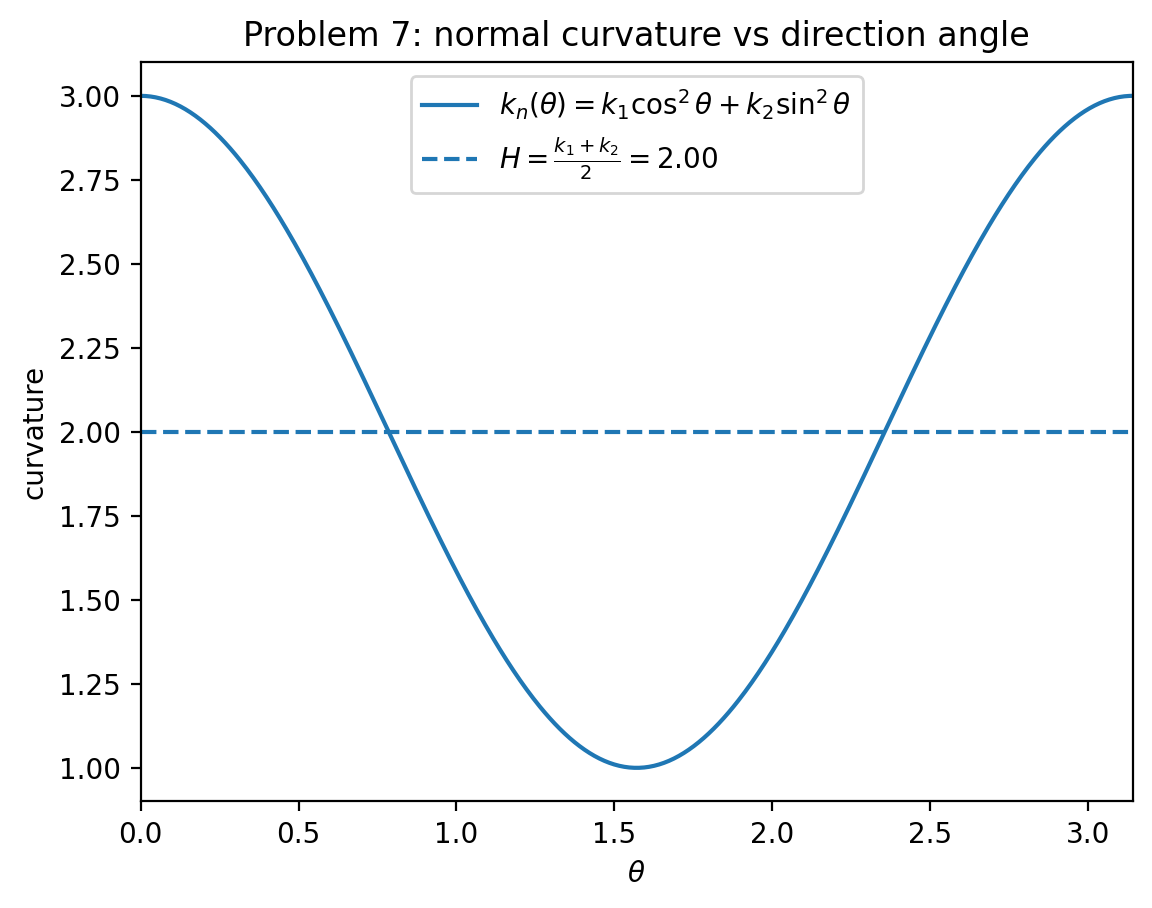
\includegraphics[width=0.72\linewidth]{chapters/part07_volume_vii/figures/problem7_kn_vs_theta.png}
	\caption{Problem 7: Normal curvature $k_n(\theta)$ versus direction angle $\theta$, with the mean curvature line $H$.}
\end{figure}

\begin{figure}[htbp]
	\centering
	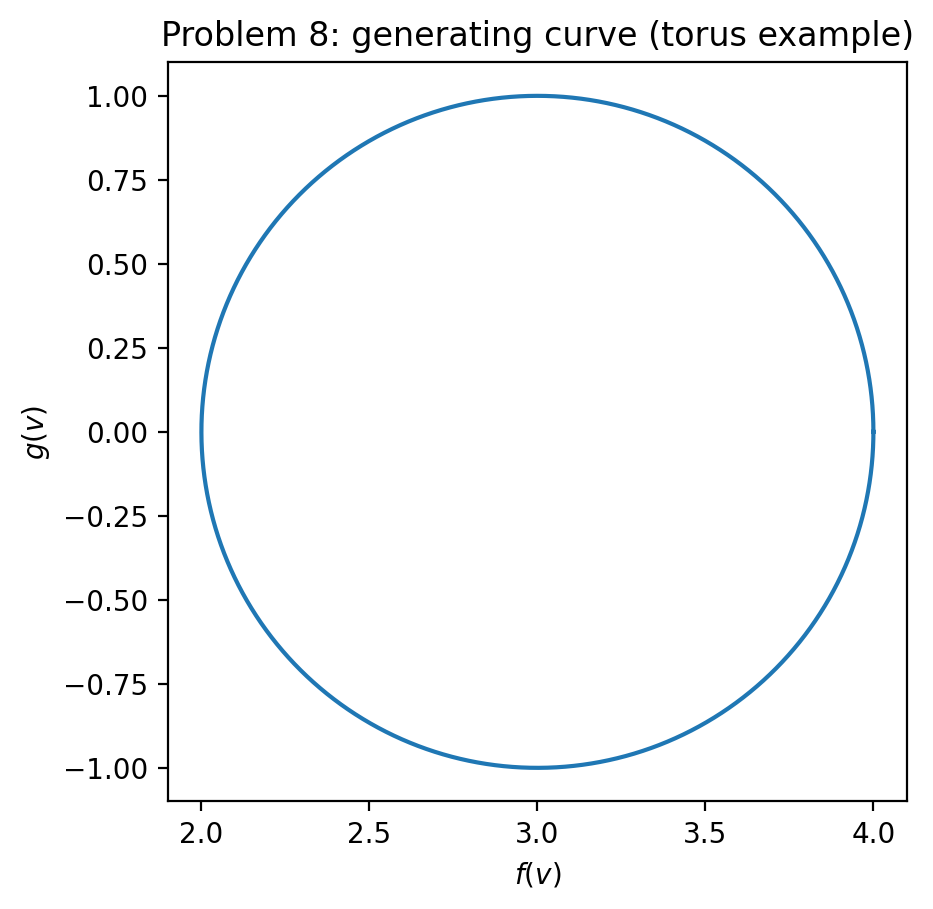
\includegraphics[width=0.62\linewidth]{chapters/part07_volume_vii/figures/problem8_generating_curve_torus.png}
	\caption{Problem 8: Example profile curve $(f(v),g(v))$ (torus). The parameter $v$ is arclength along the profile.}
\end{figure}

\begin{figure}[htbp]
	\centering
	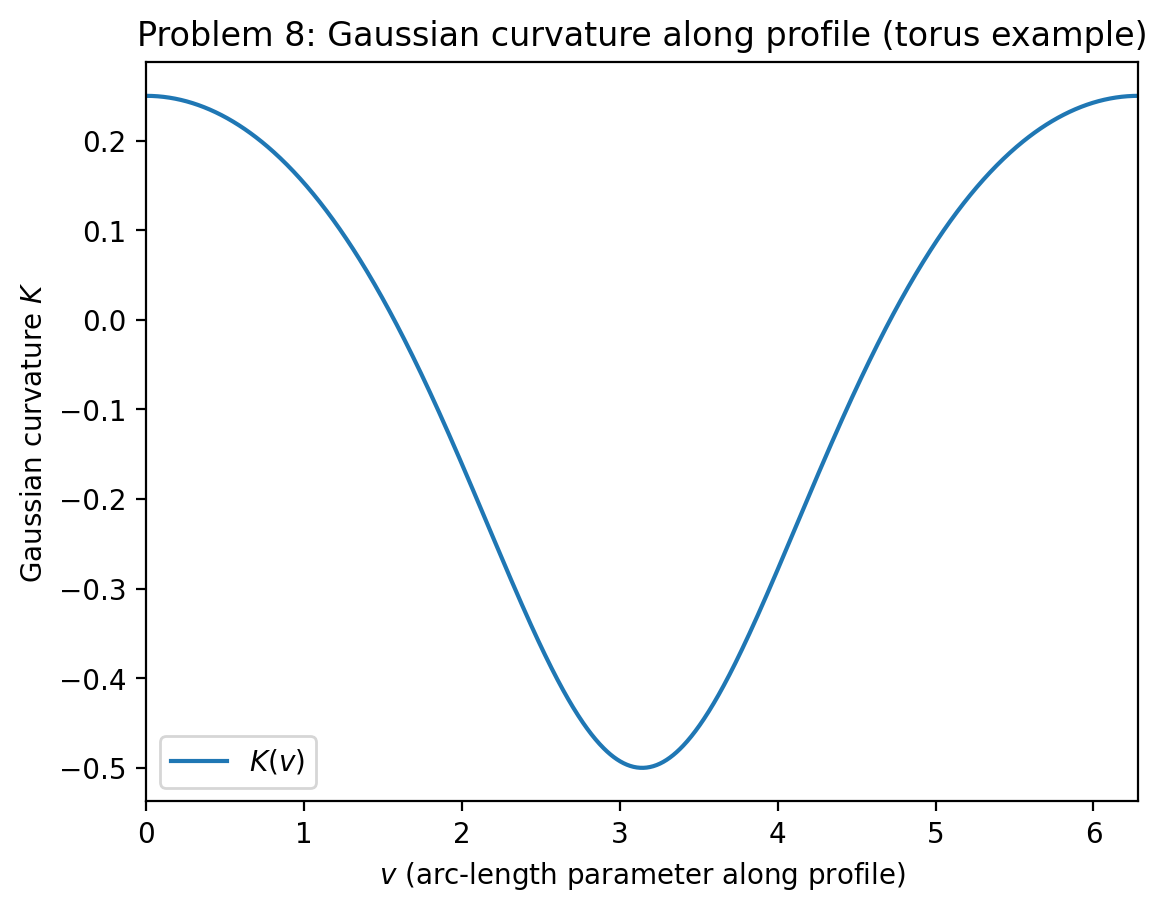
\includegraphics[width=0.72\linewidth]{chapters/part07_volume_vii/figures/problem8_K_vs_v_torus.png}
	\caption{Problem 8 (torus example): Gaussian curvature $K(v)$ along the profile parameter $v$.}
\end{figure}

\begin{figure}[htbp]
	\centering
	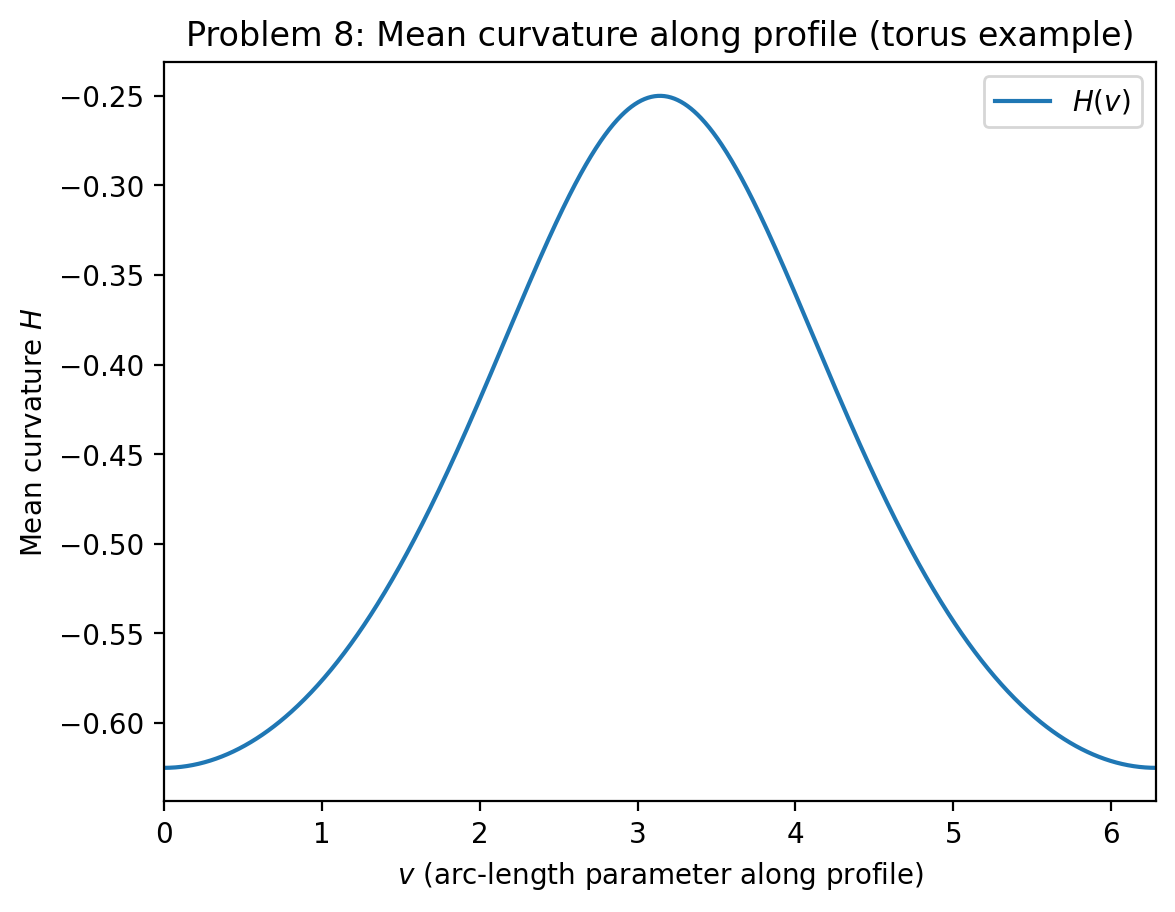
\includegraphics[width=0.72\linewidth]{chapters/part07_volume_vii/figures/problem8_H_vs_v_torus.png}
	\caption{Problem 8 (torus example): Mean curvature $H(v)$ along the profile parameter $v$.}
\end{figure}

\begin{figure}[htbp]
	\centering
	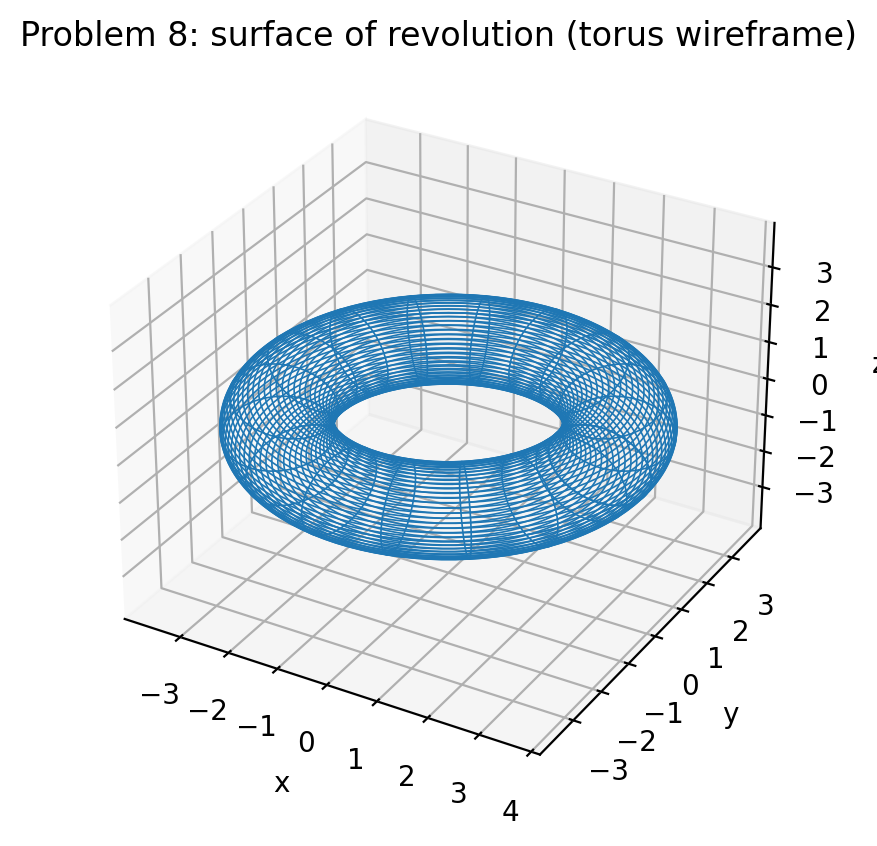
\includegraphics[width=0.78\linewidth]{chapters/part07_volume_vii/figures/problem8_torus_wireframe.png}
	\caption{Problem 8: Wireframe of the surface of revolution (torus example).}
\end{figure}

	
	\par\medskip\noindent\textbf{Arc-length parametrization of the generating curve}\par\smallskip

	The surface of revolution is obtained by rotating the planar \emph{generating (profile) curve}
	\[
	\alpha(v)=(f(v),\,g(v))\subset \mathbb{R}^2
	\]
	around the $z$-axis, producing the parametrization
	\[
	\phi(u,v)=\bigl(f(v)\cos u,\ f(v)\sin u,\ g(v)\bigr).
	\]
	Saying that the generating curve is \emph{parametrized by arc length} means that the parameter $v$
	measures distance along $\alpha$, i.e.\ the speed of $\alpha$ equals $1$:
	\[
	\|\alpha'(v)\|=1.
	\]
	Since $\alpha'(v)=(f'(v),\,g'(v))$, this is equivalent to
	\[
	\sqrt{(f'(v))^2+(g'(v))^2}=1
	\quad\Longleftrightarrow\quad
	(f'(v))^2+(g'(v))^2=1.
	\]
	Equivalently, the arc length from $v=a$ to $v=b$ is
	\[
	L=\int_a^b \|\alpha'(v)\|\,dv=\int_a^b 1\,dv=b-a.
	\]
	In particular, for the surface parametrization one gets
	\[
	G=\langle \phi_v,\phi_v\rangle=(f')^2+(g')^2=1,
	\]
	which simplifies the curvature computations.

\end{solution}

\begin{problem}[CP-VII-0052 --- Problem 10. Totally umbilic compact surfaces are planes or spheres]
\label{prob:cp-vii-0052}
Show that if $S$ is a connected surface in $\mathbb R^3$ such that every point is umbilic, then
	$S$ is contained in a plane or a sphere.
	\emph{(Hint: Use that in a parametrization $\phi(u,v)$ one has $N_{uv}=N_{vu}$.}
	
	\par\medskip\noindent\textbf{Theory}\par\smallskip

	A surface is \emph{totally umbilic} if at every point the shape operator is a scalar:
	\[
	S_p=\lambda(p)\,I.
	\]
	Equivalently, the principal curvatures satisfy $k_1=k_2=\lambda$, or $\mathrm{II}=\lambda\,\mathrm{I}$.
	In local coordinates $\phi(u,v)$ with unit normal $N$, the Weingarten equations give
	\[
	N_u=-S(\phi_u),\qquad N_v=-S(\phi_v).
	\]
\end{problem}

\begin{solution}
Assume $S$ is totally umbilic, so $S=\lambda I$. Then
	\[
	N_u=-\lambda\,\phi_u,\qquad N_v=-\lambda\,\phi_v.
	\]
	Differentiate:
	\[
	N_{uv}=-(\lambda_v\phi_u+\lambda\phi_{uv}),\qquad
	N_{vu}=-(\lambda_u\phi_v+\lambda\phi_{vu}).
	\]
	Since mixed partial derivatives commute, $N_{uv}=N_{vu}$ and $\phi_{uv}=\phi_{vu}$, hence
	\[
	\lambda_v\phi_u=\lambda_u\phi_v.
	\]
	Because $\phi_u$ and $\phi_v$ are linearly independent, it follows that
	\[
	\lambda_u=\lambda_v=0,
	\]
	so $\lambda$ is constant on each connected component; since $S$ is connected, $\lambda$ is constant.
	
	If $\lambda=0$, then $N_u=N_v=0$, so $N$ is constant and $S$ lies in a plane orthogonal to $N$.
	
	If $\lambda\neq 0$, define
	\[
	c=\phi+\frac{1}{\lambda}N.
	\]
	Then
	\[
	c_u=\phi_u+\frac{1}{\lambda}N_u=\phi_u-\phi_u=0,\qquad
	c_v=\phi_v+\frac{1}{\lambda}N_v=\phi_v-\phi_v=0,
	\]
	so $c$ is constant. Therefore $\|\phi-c\|=1/|\lambda|$, i.e.\ $\phi$ lies on a sphere of radius
	$1/|\lambda|$ centered at $c$.
	
	\par\medskip\noindent\textbf{Examples}\par\smallskip

	\begin{itemize}
		\item A plane has $k_1=k_2=0$ everywhere (totally umbilic).
		\item A sphere of radius $R$ has $k_1=k_2=\pm 1/R$ everywhere (totally umbilic).
	\end{itemize}
	
	

		
	
	% Problem 11
\end{solution}

\begin{problem}[CP-VII-0053 --- Problem 7 (Sign change of Gaussian curvature on a non-spherical compact surface)]
\label{prob:cp-vii-0053}
Let $S$ be a compact connected orientable surface in $\mathbb{R}^3$ which is not homeomorphic to a sphere.
	Prove that there are points on $S$ where the Gaussian curvature is positive, negative, and zero.
\end{problem}

\begin{solution}
\textit{Step 1: $K>0$ somewhere.}
	Fix a unit vector $v\in\mathbb{R}^3$ and consider the height function
	\[
	f:S\to\mathbb{R},\qquad f(p)=\langle p,v\rangle .
	\]
	Since $S$ is compact, $f$ attains a maximum at some $p_0\in S$.
	At a maximum, the tangential gradient vanishes, so $v$ is normal to $S$ at $p_0$.
	Moreover, the Hessian of $f$ restricted to $T_{p_0}S$ is negative semidefinite.
	Up to sign (depending on the orientation of the unit normal), this Hessian equals the second fundamental form,
	so the principal curvatures satisfy $k_1(p_0)\ge 0$ and $k_2(p_0)\ge 0$, hence $K(p_0)=k_1(p_0)k_2(p_0)\ge 0$.
	
	Choose $v$ generically so that the maximum $p_0$ is \emph{nondegenerate} (Morse), i.e.\ the Hessian is negative definite.
	Then $k_1(p_0)>0$ and $k_2(p_0)>0$, so
	\[
	K(p_0)>0.
	\]
	
	\textit{Step 2: $K<0$ somewhere.}
	Since $S$ is compact, connected, orientable, and not homeomorphic to $S^2$, it has genus $g\ge 1$ and
	\[
	\chi(S)=2-2g\le 0.
	\]
	By Gauss--Bonnet (for a closed surface),
	\[
	\int_S K\,dA \;=\; 2\pi\,\chi(S)\;\le\;0.
	\]
	But $K>0$ at $p_0$, so $K$ cannot be nonnegative everywhere unless the integral were $>0$ or (in genus $1$) could not balance to $0$.
	More precisely:
	\begin{itemize}
		\item If $g\ge 2$, then $2\pi\chi(S)<0$, so necessarily $K<0$ somewhere.
		\item If $g=1$, then $\int_S K\,dA=0$, but since $K>0$ somewhere, there must be points where $K<0$ to cancel the positive contribution.
	\end{itemize}
	Thus $K<0$ somewhere on $S$.
	
	\textit{Step 3: $K=0$ somewhere.}
	The function $K:S\to\mathbb{R}$ is continuous and $S$ is connected.
	Since $K$ takes both positive and negative values, by the intermediate value theorem there exists $p\in S$ such that
	\[
	K(p)=0.
	\]
	This proves that $K$ is positive, negative, and zero at some points of $S$.
	
	\par\medskip\noindent\textbf{Examples.}\par\smallskip

	\begin{itemize}
		\item A standard torus of revolution in $\mathbb{R}^3$ has regions with $K>0$ (outer side), $K<0$ (inner neck),
		and $K=0$ along two parabolic circles separating them.
		\item A smooth embedded genus-$2$ surface (``double torus'') similarly has elliptic regions ($K>0$), saddle regions ($K<0$),
		and parabolic curves ($K=0$).
	\end{itemize}
\end{solution}

\subsection*{Main-text correspondence: VII/18}

\begin{problem}[CP-VII-0054 --- Problem 8 -- A ruled surface with negative Gauss curvature]
\label{prob:cp-vii-0054}
Consider the surface $\Sigma \subset \mathbb{R}^3$ with parametrization
\[
\sigma(u,v)=\gamma(u)+v\,a(u),\qquad
u\in[0,2\pi),\; v\in(-1,1),
\]
where
\[
\gamma(u)=(\cos u,\;\sin u,\;0),\qquad
a(u)=\bigl(\cos\tfrac u2\cos u,\;\cos\tfrac u2\sin u,\;\sin\tfrac u2\bigr).
\]
(This is an example of a \emph{ruled surface}: one which is locally swept out
by a moving Euclidean straight line.)

\begin{enumerate}
	\item Sketch $\Sigma$.
	\item Prove that $\Sigma$ is a smooth surface.
	\item Show that the Gauss curvature $\kappa$ of $\Sigma$ is everywhere negative.
\end{enumerate}

\par\medskip\noindent\textbf{Theory.}\par\smallskip

A parametrized surface $\sigma(u,v)$ is \emph{regular} if
$\sigma_u\times\sigma_v\neq 0$ everywhere.
The first fundamental form has coefficients
\[
E=\sigma_u\cdot\sigma_u,\quad
F=\sigma_u\cdot\sigma_v,\quad
G=\sigma_v\cdot\sigma_v.
\]
The second fundamental form has coefficients
\[
e=\sigma_{uu}\cdot n,\quad
f=\sigma_{uv}\cdot n,\quad
g=\sigma_{vv}\cdot n,
\]
where $n=\dfrac{\sigma_u\times\sigma_v}{|\sigma_u\times\sigma_v|}$ is the unit normal.
The Gauss curvature is
\[
K=\frac{eg-f^2}{EG-F^2}.
\]

For convenience one may use triple products:
\[
e = \frac{\sigma_{uu}\cdot(\sigma_u\times\sigma_v)}{|\sigma_u\times\sigma_v|},\quad
f = \frac{\sigma_{uv}\cdot(\sigma_u\times\sigma_v)}{|\sigma_u\times\sigma_v|},\quad
g = \frac{\sigma_{vv}\cdot(\sigma_u\times\sigma_v)}{|\sigma_u\times\sigma_v|}.
\]
\end{problem}

\begin{solution}
\par\medskip\noindent\textbf{Geometry.}\par\smallskip

The base curve $\gamma(u)=(\cos u,\sin u,0)$ is the unit circle in the $xy$-plane.
For each fixed $u$, the map $v\mapsto \sigma(u,v)=\gamma(u)+v a(u)$ is a straight
line through $\gamma(u)$ with direction $a(u)$.
The vector $a(u)$ has length $1$, so $\Sigma$ is a ruled surface obtained by
moving a unit line along the circle.  Geometrically, $\Sigma$ looks like a
``saddle-shaped ring'' wrapped around the circle.

\par\medskip\noindent\textbf{Regularity.}\par\smallskip

We have
\[
\sigma_u=\gamma'(u)+v a'(u),\qquad
\sigma_v=a(u),
\]
with
\[
\gamma'(u)=(-\sin u,\cos u,0).
\]
A straightforward computation gives that
\[
\bigl(\sigma_u\times\sigma_v\bigr)_3
=-(v\cos\tfrac u2+1)\cos\tfrac u2.
\]
For $u\neq \pi$ we have $\cos\tfrac u2\neq 0$, and since $|v|<1$,
the expression $v\cos\tfrac u2 + 1$ cannot vanish.  Thus the third
component is non-zero.

For $u=\pi$, one checks explicitly that
\[
\sigma_u\times\sigma_v\big|_{u=\pi}=(-1,-\tfrac v2,0)\neq 0.
\]
Therefore $\sigma_u\times\sigma_v\neq 0$ for all $(u,v)$ in the domain,
and $\sigma$ is a regular parametrization. Hence $\Sigma$ is a smooth surface.

\par\medskip\noindent\textbf{First fundamental form.}\par\smallskip

Because $|a(u)|\equiv 1$, differentiating $a\cdot a=1$ yields
$a'(u)\cdot a(u)=0$.
A direct computation also gives
\[
\gamma'(u)\cdot a(u)=0.
\]
Therefore
\[
F = \sigma_u\cdot\sigma_v
= (\gamma'(u)+v a'(u))\cdot a(u)
= \gamma'(u)\cdot a(u) + v a'(u)\cdot a(u) = 0.
\]

Next,
\[
E = \sigma_u\cdot\sigma_u
= |\gamma'(u)+v a'(u)|^2
= |\gamma'(u)|^2 + 2v\,\gamma'(u)\cdot a'(u) + v^2|a'(u)|^2.
\]
One finds
\[
|\gamma'(u)|^2 = 1,\qquad
\gamma'(u)\cdot a'(u) = \cos\tfrac u2,\qquad
|a'(u)|^2 = \frac{\cos u}{2} + \frac34,
\]
so
\[
E(u,v) = 1 + 2v\cos\tfrac u2
+ v^2\left(\frac{\cos u}{2}+\frac34\right) > 0.
\]

Finally,
\[
G = \sigma_v\cdot\sigma_v = a(u)\cdot a(u) = 1.
\]

Thus the first fundamental form is
\[
I = E\,du^2 + G\,dv^2,\qquad
E>0,\; G=1,\; F=0.
\]

\par\medskip\noindent\textbf{Second fundamental form and Gauss curvature.}\par\smallskip

Second derivatives are
\[
\sigma_{uu}=\gamma''(u)+v a''(u),\qquad
\sigma_{uv}=a'(u),\qquad
\sigma_{vv}=0.
\]
Hence $g=\sigma_{vv}\cdot n=0$.

Let $N=\sigma_u\times\sigma_v$.
Then
\[
f = \frac{\sigma_{uv}\cdot N}{|N|}
= \frac{a'(u)\cdot N}{|N|}.
\]
Since $N=(\gamma'(u)+v a'(u))\times a(u)$, we obtain
\[
a'(u)\cdot N
= a'(u)\cdot\bigl(\gamma'(u)\times a(u)\bigr)
+ v\,a'(u)\cdot\bigl(a'(u)\times a(u)\bigr)
= a'(u)\cdot\bigl(\gamma'(u)\times a(u)\bigr),
\]
because $x\cdot(x\times y)=0$.

A direct computation shows
\[
\gamma'(u)\times a(u)
=\bigl(\sin\tfrac u2\cos u,\;\sin\tfrac u2\sin u,\;-\cos\tfrac u2\bigr),
\]
and
\[
a'(u)\cdot\bigl(\gamma'(u)\times a(u)\bigr)=-\frac12.
\]
Therefore
\[
\sigma_{uv}\cdot(\sigma_u\times\sigma_v) = -\frac12
\]
for all $(u,v)$, and hence
\[
f = -\frac{1}{2|N|}.
\]

Since $F=0$ and $G=1$, we know
\[
|N|^2 = EG-F^2 = E,
\]
so $|N|=\sqrt{E}$ and
\[
f = -\frac{1}{2\sqrt{E}},\qquad g=0.
\]

The Gauss curvature is
\[
K = \frac{eg-f^2}{EG-F^2}.
\]
Because $g=0$, we get
\[
K = -\frac{f^2}{EG-F^2}
= -\frac{\displaystyle\frac{1}{4E}}{E}
= -\frac{1}{4E^2}.
\]

Since $E(u,v)>0$ everywhere, it follows that
\[
K(u,v)<0\quad\text{for all }(u,v)\in[0,2\pi)\times(-1,1).
\]
Thus the Gaussian curvature of $\Sigma$ is everywhere negative.

\par\medskip\noindent\textbf{Examples.}\par\smallskip

This surface is a non-developable ruled surface with strictly negative
Gaussian curvature.  Other examples of ruled surfaces with $K<0$ include
the helicoid and the hyperbolic paraboloid.  In contrast, cylinders and
cones are ruled surfaces with $K=0$.

\par\medskip\noindent\textbf{E1 -- Strictly convex surfaces and the convex Gauss--Bonnet theorem}\par\smallskip


\textbf{Problem.}
A compact smooth surface $\Sigma \subset \mathbb{R}^3$ is \emph{strictly convex}
if it is the boundary of a closed region $R \subset \mathbb{R}^3$ with the
property that for any $x,y \in R$, the straight line segment $[x,y] \subset R$,
and
\[
[x,y] \cap \Sigma \subset \{x,y\}.
\]
Show that the Gauss map of a strictly convex surface $\Sigma$ is a bijection.
If, furthermore, the Gauss curvature $\kappa$ of $\Sigma$ is everywhere
positive, show that the Gauss map is a diffeomorphism, and deduce that
\[
\int_{\Sigma} \kappa\, dA = 4\pi,
\]
where $\kappa$ is the Gauss curvature and $dA$ is the area form on $\Sigma$.
\emph{(This is the `convex' Gauss--Bonnet theorem.)}

\par\medskip\noindent\textbf{Theory.}\par\smallskip

For an oriented smooth surface $\Sigma\subset\mathbb{R}^3$ the Gauss map
\[
N:\Sigma\to S^2,\qquad N(p)=\text{unit normal at }p,
\]
is smooth.  Its differential
$dN_p:T_p\Sigma\to T_{N(p)}S^2$ is (up to sign) the shape operator, and
\[
\det(dN_p)=\kappa(p)
\]
is the Gauss curvature.  If $N$ is a diffeomorphism then
\[
N^*(dA_{S^2}) = \det(dN_p)\,dA = \kappa\, dA,
\]
so by change of variables,
\[
\int_\Sigma \kappa\,dA
= \int_\Sigma N^*(dA_{S^2})
= \int_{S^2} dA_{S^2}
= \operatorname{Area}(S^2) = 4\pi.
\]

\par\medskip\noindent\textbf{Solution.}\par\smallskip


\par\medskip\noindent\textbf{Gauss map is a bijection.}\par\smallskip

Fix a unit vector $n\in S^2$ and consider the function
\[
h:\Sigma\to\mathbb{R},\qquad h(x)=x\cdot n.
\]
Since $\Sigma$ is compact, $h$ attains a maximum at some $p\in\Sigma$.
At such a maximum the gradient of $h$ is orthogonal to $T_p\Sigma$, so $n$
is parallel to the normal vector at $p$.  Choosing the orientation so that
normals point outward, we get $N(p)=n$.  Hence $N$ is surjective.

To show injectivity, suppose $N(p_1)=N(p_2)=n$ for some $p_1\neq p_2$.
Let $c=p_1\cdot n=p_2\cdot n$ and consider the plane
\[
P=\{x\in\mathbb{R}^3 : x\cdot n = c\}.
\]
Since $R$ is convex and $n$ is an outward normal, $R\subset\{x\cdot n\le c\}$,
and $P$ is a supporting plane to $R$.  The segment $[p_1,p_2]$ lies entirely
in $P$ and in $R$.  Near any point of $[p_1,p_2]$, $R$ lies on one side
of $P$, so every interior point of $[p_1,p_2]$ is on the boundary of $R$,
i.e.\ belongs to $\Sigma$.  Thus
\[
[p_1,p_2]\cap\Sigma
\]
contains more than just the endpoints, contradicting strict convexity.
Therefore $p_1=p_2$, and $N$ is injective.

Hence for a strictly convex surface $\Sigma$ the Gauss map
$N:\Sigma\to S^2$ is bijective.

\par\medskip\noindent\textbf{Gauss map is a diffeomorphism if $\kappa>0$.}\par\smallskip

We already know $N$ is smooth and bijective.  At each $p\in\Sigma$,
\[
\det(dN_p)=\kappa(p).
\]
If $\kappa(p)>0$ for all $p$, then $dN_p$ is invertible for every $p$.
Thus $N$ is a local diffeomorphism.

A smooth bijective local diffeomorphism between compact manifolds of the
same dimension is a global diffeomorphism.  Consequently, when
$\kappa>0$ everywhere, the Gauss map
\[
N:\Sigma\stackrel{\cong}{\longrightarrow} S^2
\]
is a diffeomorphism.

\par\medskip\noindent\textbf{Integral of Gauss curvature.}\par\smallskip

Let $dA_{S^2}$ denote the area form on the unit sphere.
Because $N$ is a diffeomorphism, we have
\[
N^*(dA_{S^2}) = \det(dN_p)\,dA = \kappa\, dA.
\]
Integrating and using change of variables,
\[
\int_\Sigma \kappa\,dA
= \int_\Sigma N^*(dA_{S^2})
= \int_{S^2} dA_{S^2}
= \operatorname{Area}(S^2)
= 4\pi.
\]
This proves the convex Gauss--Bonnet formula for strictly convex surfaces
with everywhere positive Gauss curvature.

\par\medskip\noindent\textbf{Examples.}\par\smallskip

The surface in the problem is a non--developable ruled surface with strictly
negative Gaussian curvature: its parametrisation
\[
\sigma(u,v)=\gamma(u)+v\,a(u),\qquad
\gamma(u)=(\cos u,\sin u,0),\quad
a(u)=\Bigl(\cos\frac u2\cos u,\cos\frac u2\sin u,\sin\frac u2\Bigr),
\]
yields Gauss curvature
\[
K(u,v)=-\frac{1}{4E(u,v)^2}<0.
\]

Other ruled surfaces with $K<0$ include:


These examples illustrate that ruled surfaces can have strictly negative
Gaussian curvature (helicoid, hyperbolic paraboloid, the example in the
problem) or vanishing curvature (cylinders and cones).


\begin{enumerate}
	\item \textbf{Our ruled surface from the problem}
	
	\emph{Chart}
	\[
	\sigma(u,v)=\gamma(u)+v\,a(u),\qquad
	\gamma(u)=(\cos u,\sin u,0),\qquad
	a(u)=\Bigl(\cos\frac u2\cos u,\;\cos\frac u2\sin u,\;\sin\frac u2\Bigr).
	\]
	Each line $v\mapsto\sigma(u,v)$ is a ruling.
	
	\smallskip
	\emph{Curvature}
	We computed
	\[
	K(u,v)=-\frac{1}{4E(u,v)^2}<0,
	\]
	so this is a \emph{non-developable} ruled surface with strictly negative
	Gaussian curvature.
	
	\item \textbf{Helicoid -- ruled with $K<0$}
	
	\emph{Chart}
	\[
	\sigma(u,v)=(v\cos u,\;v\sin u,\;a u),\qquad
	u\in\mathbb{R},\ v\in\mathbb{R},\ a>0.
	\]
	For fixed $u$, $v\mapsto\sigma(u,v)$ is a straight line (a radial line in a
	horizontal plane); as $u$ changes, the line twists upwards -- a ``spiral
	ramp''.
	
	\smallskip
	\emph{Curvature} (standard formula)
	\[
	K(u,v)=-\frac{a^{2}}{(a^{2}+v^{2})^{2}}<0.
	\]
	So the helicoid is a classic example of a ruled surface with negative Gauss
	curvature.
	
	\item \textbf{Hyperbolic paraboloid -- ruled with $K<0$}
	
	Take the saddle surface
	\[
	z = x\,y.
	\]
	
	\emph{Chart}
	\[
	\sigma(u,v)=(u,\;v,\;u v).
	\]
	For fixed $u=u_0$, this is the straight line
	$(u_0,0,0)+v(0,1,u_0)$; for fixed $v=v_0$, it is
	$(0,v_0,0)+u(1,0,v_0)$.  Thus the hyperbolic paraboloid is doubly ruled.
	
	\smallskip
	\emph{Curvature}
	\[
	K(u,v)=-\frac{1}{(1+u^{2}+v^{2})^{2}}<0.
	\]
	
	\item \textbf{Circular cylinder -- ruled with $K=0$}
	
	\emph{Chart}
	\[
	\sigma(u,v)=(\cos u,\;\sin u,\;v),\qquad
	u\in[0,2\pi),\ v\in\mathbb{R}.
	\]
	For fixed $u$, $v\mapsto\sigma(u,v)$ is a straight vertical line, so the
	cylinder is ruled.
	
	\smallskip
	\emph{Curvature}
	A direct computation gives
	\[
	K(u,v)=0.
	\]
	Cylinders are ruled and \emph{developable} (locally isometric to the plane).
	
	\item \textbf{Right circular cone -- ruled with $K=0$ (off the tip)}
	
	\emph{Chart}
	\[
	\sigma(u,v)=(v\cos u,\;v\sin u,\;v),\qquad
	u\in[0,2\pi),\ v>0.
	\]
	For fixed $u$, $v\mapsto\sigma(u,v)$ is a straight ray from the apex, so the
	cone is ruled.
	
	\smallskip
	\emph{Curvature}
	Away from the apex one finds
	\[
	K(u,v)=0.
	\]
	The vertex is a singular point (not part of a smooth surface), but on the
	smooth part the cone is developable.
\end{enumerate}	
	
	
	\par\medskip\noindent\textbf{Ruled, developable and (strictly) convex surfaces}\par\smallskip

	
	\par\medskip\noindent\textbf{Ruled surfaces.}\par\smallskip

	A smooth surface $\Sigma\subset\mathbb{R}^3$ is called \emph{ruled} if through
	every point $p\in\Sigma$ there passes at least one straight line (a
	\emph{ruling}) that lies entirely in $\Sigma$.
	
	A typical local parametrisation of a ruled surface is
	\[
	\sigma(u,v)=c(u)+v\,d(u),
	\]
	where $c(u)$ is a space curve (the \emph{directrix}) and $d(u)$ is a (usually
	unit) direction vector.  For each fixed $u$, the map $v\mapsto\sigma(u,v)$ is a
	straight line.
	
	Examples:
	\begin{itemize}
		\item Plane: $\sigma(u,v)=(u,v,0)$.
		\item Circular cylinder: $\sigma(u,v)=(\cos u,\sin u,v)$.
		\item Cone (away from the tip): $\sigma(u,v)=(v\cos u,v\sin u,v)$.
		\item Helicoid: $\sigma(u,v)=(v\cos u,v\sin u,au)$.
		\item Hyperbolic paraboloid: $\sigma(u,v)=(u,v,uv)$.
	\end{itemize}
	Thus ``ruled'' means ``built from straight lines''; it does \emph{not} by itself
	impose any condition on the curvature.
	
	\bigskip
	\par\medskip\noindent\textbf{Developable surfaces.}\par\smallskip

	A surface $\Sigma$ is called \emph{developable} if it can be unfolded onto the
	plane without stretching or tearing, i.e.\ if it is locally isometric to the
	plane.  For regular surfaces in $\mathbb{R}^3$ this is equivalent to
	\emph{vanishing Gaussian curvature}:
	\[
	K\equiv 0 \quad\Longleftrightarrow\quad
	\text{$\Sigma$ is (locally) developable}.
	\]
	
	Among ruled surfaces one has the classical classification: a smooth ruled
	surface with $K=0$ is locally a piece of a plane, a cylinder, a cone, or a
	tangent developable of a space curve.
	
	Examples of \emph{developable ruled} surfaces:
	\begin{itemize}
		\item Plane ($K=0$).
		\item Circular cylinder ($K=0$).
		\item Right circular cone away from the apex ($K=0$).
	\end{itemize}

Non-developable ruled surfaces (with $K\neq 0$, in fact $K<0$)
	include the helicoid, the hyperbolic paraboloid, and the ruled surface
	from the previous problem.
	
	\bigskip
	\par\medskip\noindent\textbf{Convex and strictly convex.}\par\smallskip

	A set $R\subset\mathbb{R}^3$ is \emph{convex} if for any $x,y\in R$ the whole
	segment $[x,y]$ is contained in $R$:
	\[
	x,y\in R \quad\Rightarrow\quad [x,y]\subset R.
	\]
	A compact smooth surface $\Sigma$ is called \emph{convex} if it is the boundary
	of a convex region $R$.
	
	Typical convex (but not strictly convex) examples: cubes, cylinders, prisms;
	their boundaries contain flat faces or flat strips.
	
	\medskip
	In the exercise, a compact smooth surface $\Sigma=\partial R$ is called
	\emph{strictly convex} if $R$ is convex and, in addition,
	\[
	x,y\in R \quad\Rightarrow\quad [x,y]\subset R
	\quad\text{and}\quad [x,y]\cap\Sigma\subset\{x,y\}.
	\]
	In words: no nontrivial line segment lies on the boundary; the only points of
	$\Sigma$ on any chord $[x,y]$ are the endpoints.  Thus the boundary has no flat
	pieces or straight edges: it ``bulges outward'' everywhere.
	
	Typical strictly convex examples: spheres, ellipsoids, smooth ``rounded''
	convex bodies.
	
	\medskip
	Clearly,
	\[
	\text{strictly convex} \;\Longrightarrow\; \text{convex},
	\]
	but the converse fails (a cylinder is convex but not strictly convex).  For
	smooth surfaces, strict convexity rules out flat regions on $\Sigma$; in
	particular, one expects the principal curvatures to be positive everywhere and
	hence $K>0$.  In the exercise, the assumptions
	\[
	\Sigma\ \text{strictly convex}, \qquad K>0
	\]
	are used to show that the Gauss map is bijective and has everywhere-invertible
	differential, hence is a diffeomorphism.
\end{solution}

\subsection*{Main-text correspondence: VII/19}

\begin{problem}[CP-VII-0055 --- Problem 6 (Minimal surfaces and conformality of the Gauss map)]
\label{prob:cp-vii-0055}
Let $S$ be a regular surface without umbilical points. Prove that $S$ is minimal iff the Gauss map
	$N:S\to S^2$ satisfies
	\[
	\langle dN_p(v_1), dN_p(v_2)\rangle = \lambda(p)\,\langle v_1,v_2\rangle
	\]
	for all $p\in S$ and all $v_1,v_2\in T_pS$, where $\lambda(p)\neq 0$ depends only on $p$.
	By considering stereographic projection deduce that isothermal coordinates exist around a nonplanar point
	in a minimal surface.
	
	\medskip
\end{problem}

\begin{solution}
Let $S_p:T_pS\to T_pS$ be the shape operator. The Weingarten relation is
	\[
	dN_p(v)=-S_p(v).
	\]
	Thus the condition becomes
	\[
	\langle S_p(v_1), S_p(v_2)\rangle = \lambda(p)\,\langle v_1,v_2\rangle
	\qquad(\lambda(p)\neq 0).
	\]
	Choose an orthonormal principal basis $(e_1,e_2)$ at $p$, so $S_p(e_i)=k_i e_i$ where $k_1,k_2$ are the
	principal curvatures. Writing $v=a_1e_1+a_2e_2$ and $w=b_1e_1+b_2e_2$,
	\[
	\langle S_p(v),S_p(w)\rangle = k_1^2 a_1b_1 + k_2^2 a_2b_2,\qquad
	\langle v,w\rangle = a_1b_1+a_2b_2.
	\]
	Since the identity holds for all $v,w$, it follows that $k_1^2=k_2^2=\lambda(p)$.
	Because $S$ has no umbilics we have $k_1\neq k_2$, hence $k_2=-k_1\neq 0$.
	Therefore
	\[
	H(p)=\frac{k_1+k_2}{2}=0,
	\]
	so $S$ is minimal.
	
	Conversely, if $S$ is minimal and has no umbilics, then $k_2=-k_1\neq 0$, hence $k_1^2=k_2^2$ and the
	identity holds with $\lambda(p)=k_1(p)^2=-K(p)>0$.
	
	\medskip
	For the isothermal coordinates: on a minimal surface (without umbilics at the point considered) the Gauss map
	$N$ is conformal, and at a nonplanar point $p$ we have $dN_p\neq 0$.
	Stereographic projection $\pi:S^2\setminus\{\text{north pole}\}\to\mathbb C$ is conformal, hence
	$g=\pi\circ N$ is conformal. Since $dN_p\neq 0$, $g$ is a local diffeomorphism near $p$.
	Writing $g=u+iv$, the coordinates $(u,v)$ are isothermal, i.e.
	\[
	ds^2 = \rho(u,v)^2(du^2+dv^2)
	\]
	for some positive function $\rho$.
	\qed
	
	
	\par\medskip\noindent\textbf{Where does $dN_p$ come from?}\par\smallskip

	The Gauss map is $N:S\to S^2$, $N(p)=\text{unit normal at }p$.
	Its differential at $p$ is the linear map
	\[
	dN_p:T_pS\to T_{N(p)}S^2,
	\]
	defined by: for $v\in T_pS$, choose a smooth curve $\gamma(t)\subset S$ with
	$\gamma(0)=p$ and $\gamma'(0)=v$, and set
	\[
	dN_p(v)=\left.\frac{d}{dt}\right|_{0}N(\gamma(t)).
	\]
	Since $\|N(\gamma(t))\|^2=1$, differentiating gives
	$\langle N(p),dN_p(v)\rangle=0$, hence $dN_p(v)\in T_{N(p)}S^2$.
	Moreover, the shape operator is $S_p=-dN_p$ (via the natural identification of tangent planes in $\mathbb{R}^3$),
	so $dN_p$ encodes the principal curvatures.
	
	\par\medskip\noindent\textbf{Two normals and orientability.}\par\smallskip

	At each $p\in S\subset\mathbb{R}^3$ the normal line is 1-dimensional, hence there are exactly two unit normals:
	$N(p)$ and $-N(p)$. A \emph{Gauss map} is a choice of one of these at every point,
	i.e.\ a map $N:S\to S^2$ with $N(p)\perp T_pS$.
	
	A surface is \emph{orientable} iff one can choose the unit normal \emph{continuously} (equivalently smoothly) on all of $S$,
	i.e.\ iff there exists a global smooth Gauss map $N:S\to S^2$.
	Non-orientability means that local choices of normal exist on charts but necessarily flip sign on some overlaps/loops.
	
	If $X(u,v)$ is a local parametrization, a local unit normal is
	\[
	N=\frac{X_u\times X_v}{\|X_u\times X_v\|}.
	\]
	On an overlap of two charts, the corresponding normals differ by a sign given by the Jacobian of the coordinate change:
	the normal flips when the change of coordinates reverses orientation.
	
	Finally, choosing the opposite normal replaces $N$ by $-N$ and $dN_p$ by $-dN_p$, but
	\[
	\langle dN_p(v_1),dN_p(v_2)\rangle
	\]
	is unchanged, so conformality statements are independent of the sign choice.
\end{solution}

\begin{problem}[CP-VII-0056 --- Problem 10. Associated family in Weierstrass data (local isometry)]
\label{prob:cp-vii-0056}
\par\medskip\noindent\textbf{\textbf{Problem statement.}}\par\smallskip

The Weierstrass representation is not unique: if $\phi_{(f,g)}:D\to\mathbb{R}^3$ is the associated parametrization and
$\alpha:W\to D$ is a bijective holomorphic map, then $\phi_{(f,g)}\circ\alpha$ is another representation of the same minimal
surface and it must have the same form with different $f$ and $g$ (which should be specified).
By choosing $\alpha(z)=g^{-1}(z)$, show that, locally around regular points of $g$ (where $g'\neq 0$), we can assume
that our pair $(f,g)$ is of the form $(F,\mathrm{id})$, for some local holomorphic function $F$. We denote such a
representation by $\phi_F$. Show that the minimal surfaces given by $\phi_{e^{-i\theta}F}$ for $\theta\in\mathbb{R}$
are all locally isometric.

\medskip

\par\medskip\noindent\textbf{Theory / setup}\par\smallskip

We use the Weierstrass data $(f,g)$ (holomorphic on $D$, with $g$ meromorphic in general) in the form
\[
\phi_{(f,g)}(z)
=
\Re\int^z
\Bigl(\tfrac12 f(1-g^2),\ \tfrac{i}{2}f(1+g^2),\ fg\Bigr)\,dz.
\]
Its induced metric is
\[
ds^2
=
\frac{|f|^2(1+|g|^2)^2}{4}\,|dz|^2.
\]

\medskip
\end{problem}

\begin{solution}
Let $\alpha:W\to D$ be biholomorphic and consider $\phi_{(f,g)}\circ\alpha$. Writing $z=\alpha(w)$, we have
$dz=\alpha'(w)\,dw$, hence
\[
\phi_{(f,g)}(\alpha(w))
=
\Re\int^w
\Bigl(\tfrac12 f(\alpha(\xi))(1-g(\alpha(\xi))^2),\ \tfrac{i}{2}f(\alpha(\xi))(1+g(\alpha(\xi))^2),\ f(\alpha(\xi))g(\alpha(\xi))\Bigr)
\,\alpha'(\xi)\,d\xi.
\]
Therefore $\phi_{(f,g)}\circ\alpha$ is again a Weierstrass representation with new data
\[
\tilde g(w)=g(\alpha(w)),\qquad
\tilde f(w)=f(\alpha(w))\,\alpha'(w).
\]

Now assume $g'(z_0)\neq 0$. By the holomorphic inverse function theorem, there is a neighborhood on which $g$ admits a
holomorphic inverse $g^{-1}$. Choose $\alpha=g^{-1}$. Then locally
\[
\tilde g(w)=g(g^{-1}(w))=w=\mathrm{id}(w),
\qquad
\tilde f(w)= f(g^{-1}(w))\,(g^{-1})'(w)=:F(w),
\]
so the pair has the form $(F,\mathrm{id})$. We denote the corresponding immersion by $\phi_F$.

Finally, for $g(z)=z$ the induced metric becomes
\[
ds^2=\frac{|F(z)|^2(1+|z|^2)^2}{4}\,|dz|^2.
\]
Replacing $F$ by $e^{-i\theta}F$ does not change $|F|$, hence produces the same metric. Thus the identity map on the
parameter domain is a local isometry between $\phi_F$ and $\phi_{e^{-i\theta}F}$. Therefore the family
$\{\phi_{e^{-i\theta}F}\}_{\theta\in\mathbb{R}}$ consists of locally isometric minimal surfaces.

\medskip

\par\medskip\noindent\textbf{Examples}\par\smallskip

\begin{enumerate}
	\item \textbf{Catenoid--helicoid associated family (classical).}
	Take $g(z)=z$ and $f(z)=1/z^2$ (on a punctured domain). Then $f_\theta(z)=e^{-i\theta}/z^2$ yields the associated family.
	In particular, $\theta=0$ gives (a parametrization of) the catenoid and $\theta=\pi/2$ gives (a parametrization of) the
	helicoid, and they are locally isometric since the induced metric depends only on $|f_\theta|=|f|$.
	
	\item \textbf{Enneper associated family.}
	Take $g(z)=z$ and $f(z)=1$ (on a simply connected domain). Then $f_\theta=e^{-i\theta}$ produces the associated Enneper
	family, all locally isometric for the same reason.
\end{enumerate}

\medskip

\par\medskip\noindent\textbf{Theory: Weierstrass data, metric, and reparametrization}\par\smallskip

Let $D\subset\mathbb C$ be simply connected and let $(f,g)$ be holomorphic data (with $g$ meromorphic in general).
Define the $\mathbb C^3$-valued holomorphic $1$-form
\[
\Phi_{(f,g)}(z)\,dz
=
\Bigl(\tfrac12 f(1-g^2),\ \tfrac{i}{2}f(1+g^2),\ fg\Bigr)\,dz.
\]
The associated minimal immersion is given by
\[
\phi_{(f,g)}(z)=\Re\int^z \Phi_{(f,g)}(\zeta)\,d\zeta.
\]
The choice of $\Phi_{(f,g)}$ ensures $\Phi_{(f,g)}\cdot\Phi_{(f,g)}=0$ (complex bilinear dot product), so the parametrization is
conformal, and holomorphicity implies the coordinate functions are harmonic; hence $\phi_{(f,g)}$ is minimal.

\smallskip
The induced metric (first fundamental form) of $\phi_{(f,g)}$ is conformal:
\[
ds^2
=
2\langle \phi_z,\phi_{\bar z}\rangle\,|dz|^2
=
\frac{|f|^2(1+|g|^2)^2}{4}\,|dz|^2.
\]
In particular, the metric depends only on $|f|$ and $|g|$. Thus multiplying $f$ by a unimodular constant
$e^{-i\theta}$ leaves $ds^2$ unchanged.

\smallskip
Non-uniqueness arises from holomorphic reparametrization.
If $\alpha:W\to D$ is biholomorphic and we reparametrize by $z=\alpha(w)$, then $dz=\alpha'(w)\,dw$ and
$\phi_{(f,g)}\circ\alpha$ is again a Weierstrass immersion with new data
\[
\tilde g(w)=g(\alpha(w)),
\qquad
\tilde f(w)=f(\alpha(w))\,\alpha'(w).
\]
At points where $g'(z_0)\neq 0$, the holomorphic inverse function theorem gives a local inverse $g^{-1}$.
Choosing $\alpha=g^{-1}$ yields $\tilde g=\mathrm{id}$ and $\tilde f=:F$ holomorphic, so locally one may normalize the data to
$(F,\mathrm{id})$ and write the immersion as $\phi_F$.
The family $\phi_{e^{-i\theta}F}$ ($\theta\in\mathbb R$) is called the associated family; since $|e^{-i\theta}F|=|F|$, all
members have the same induced metric and are therefore locally isometric.

\medskip

\par\medskip\noindent\textbf{Geometric interpretation}\par\smallskip

The Weierstrass data $(f,g)$ encode two geometric ingredients.

\smallskip
\emph{(1) The Gauss map.}
For a conformal minimal immersion $X=\phi_{(f,g)}$, let $N$ be the unit normal field.
The Gauss map is $N:D\to\mathbb S^2$. Composing with stereographic projection
$\sigma:\mathbb S^2\setminus\{(0,0,1)\}\to\mathbb C$ gives a (locally) meromorphic function
\[
g=\sigma\circ N.
\]
Thus $g(z)$ is the normal direction written in a complex coordinate. In particular, constant $g$ means constant normal,
hence $X$ is a plane; nonconstant $g$ corresponds to bending of the surface.

\smallskip
\emph{(2) The holomorphic $1$-form $f\,dz$.}
The differential $f(z)\,dz$ controls the conformal scale of the parametrization. The induced metric is
\[
ds^2=\frac{|f|^2(1+|g|^2)^2}{4}\,|dz|^2,
\]
so $|f|$ (together with $|g|$) determines local lengths on the surface, while the argument of $f$ represents a constant
``phase'' in the complex differential.

\smallskip
\emph{(3) Conformality and minimality.}
The $\mathbb C^3$-valued $1$-form
\[
\Phi_{(f,g)}\,dz
=
\Bigl(\tfrac12 f(1-g^2),\ \tfrac{i}{2}f(1+g^2),\ fg\Bigr)\,dz
\]
is arranged so that the complex derivative satisfies $X_z\cdot X_z=0$, which is the isotropy condition ensuring the
parametrization is conformal. Moreover each coordinate function of $X=\Re\int \Phi$ is harmonic (real part of a holomorphic
function), hence $X$ is minimal.

\smallskip
\emph{(4) Associated family.}
Multiplying $f$ by a unimodular constant $e^{-i\theta}$ rotates the holomorphic differential by a constant phase.
This generally changes the immersion in $\mathbb R^3$, but does not change the metric since $|e^{-i\theta}f|=|f|$.
Therefore $\phi_{e^{-i\theta}F}$ all share the same first fundamental form and are locally isometric.

\medskip

\par\medskip\noindent\textbf{Theory (definitions and detailed metric computation)}\par\smallskip


\smallskip
\textbf{Complex coordinate and derivatives.}
Let $z=x+iy$ on a domain $D\subset\mathbb C$. Then $|dz|^2:=dx^2+dy^2$.
We use $\partial_z=\tfrac12(\partial_x-i\partial_y)$ and $\partial_{\bar z}=\tfrac12(\partial_x+i\partial_y)$.

\smallskip
\textbf{Weierstrass $1$-form and immersion.}
Given holomorphic data $(f,g)$ (with $g$ meromorphic in general), define the $\mathbb C^3$-valued holomorphic $1$-form
\[
\Phi_{(f,g)}(z)\,dz
=
\Bigl(\tfrac12 f(1-g^2),\ \tfrac{i}{2}f(1+g^2),\ fg\Bigr)\,dz.
\]
On simply connected $D$, set $\Psi(z):=\int^z \Phi_{(f,g)}(\zeta)\,d\zeta\in\mathbb C^3$ and define the immersion
\[
\phi_{(f,g)}(z)=\Re \Psi(z)\in\mathbb R^3.
\]
We distinguish the \emph{complex bilinear} dot product $a\cdot b=\sum_{j=1}^3 a_j b_j$ from the Hermitian product
$\langle a,b\rangle=\sum_{j=1}^3 a_j\overline{b_j}$.

\smallskip
\textbf{Isotropy $\Phi\cdot\Phi=0$ (conformality).}
Write
\[
\Phi_1=\tfrac12 f(1-g^2),\qquad
\Phi_2=\tfrac{i}{2}f(1+g^2),\qquad
\Phi_3=fg.
\]
Then, using the complex bilinear dot product,
\[
\Phi\cdot\Phi=\Phi_1^2+\Phi_2^2+\Phi_3^2
=
\frac{f^2}{4}(1-g^2)^2-\frac{f^2}{4}(1+g^2)^2+f^2g^2.
\]
Since $(1-g^2)^2-(1+g^2)^2=-4g^2$, it follows that $\Phi\cdot\Phi=0$.
Moreover, $\Psi$ is holomorphic with $\Psi'(z)=\Phi(z)$, hence
\[
\phi_z=\partial_z\Re\Psi=\frac12\Psi'(z)=\frac12\Phi(z),\qquad
\phi_{\bar z}=\frac12\overline{\Phi(z)}.
\]
Therefore $\phi_z\cdot\phi_z=\tfrac14(\Phi\cdot\Phi)=0$, which is the conformality condition.

\smallskip
\textbf{Induced metric.}
In complex notation, the first fundamental form of a conformal immersion is
\[
ds^2 = 2\langle \phi_z,\phi_{\bar z}\rangle\,|dz|^2.
\]
Using $\phi_z=\tfrac12\Phi$ we get
\[
\langle \phi_z,\phi_{\bar z}\rangle
=
\left\langle \tfrac12\Phi,\tfrac12\overline{\Phi}\right\rangle
=
\frac14 \langle \Phi,\overline{\Phi}\rangle
=
\frac14|\Phi|^2,
\]
hence $ds^2=\frac{|\Phi|^2}{2}|dz|^2$, where $|\Phi|^2:=|\Phi_1|^2+|\Phi_2|^2+|\Phi_3|^2$.
Now
\[
|\Phi_1|^2=\frac{|f|^2}{4}|1-g^2|^2,\quad
|\Phi_2|^2=\frac{|f|^2}{4}|1+g^2|^2,\quad
|\Phi_3|^2=|f|^2|g|^2,
\]
so
\[
|\Phi|^2
=
\frac{|f|^2}{4}\Bigl(|1-g^2|^2+|1+g^2|^2+4|g|^2\Bigr).
\]
Expanding gives
\[
|1-g^2|^2+|1+g^2|^2 = 2(1+|g|^4),
\]
hence the bracket equals
\[
2(1+|g|^4)+4|g|^2=2(1+2|g|^2+|g|^4)=2(1+|g|^2)^2.
\]
Therefore
\[
|\Phi|^2=\frac{|f|^2}{2}(1+|g|^2)^2,
\qquad
ds^2=\frac{|\Phi|^2}{2}|dz|^2
=\frac{|f|^2(1+|g|^2)^2}{4}\,|dz|^2.
\]

\smallskip
\textbf{Why minimal.}
Each component $\Psi_k$ is holomorphic and $\phi_k=\Re\Psi_k$ is harmonic, so $\Delta\phi=0$.
For a conformal immersion, $\Delta\phi=2\lambda^2 H$ where $H$ is the mean curvature vector.
Thus $\Delta\phi=0$ implies $H=0$, i.e.\ $\phi$ is minimal.

\medskip

\par\medskip\noindent\textbf{Lemma (metric in complex notation)}\par\smallskip

Let $\phi=\phi(x,y)$ be a smooth map into $\mathbb R^3$ and set
\[
E=\langle \phi_x,\phi_x\rangle,\qquad
F=\langle \phi_x,\phi_y\rangle,\qquad
G=\langle \phi_y,\phi_y\rangle,
\]
so that the first fundamental form is
\[
ds^2=E\,dx^2+2F\,dx\,dy+G\,dy^2.
\]
Define complex derivatives
\[
\phi_z=\tfrac12(\phi_x-i\phi_y),\qquad
\phi_{\bar z}=\tfrac12(\phi_x+i\phi_y).
\]
Then
\[
\langle \phi_z,\phi_{\bar z}\rangle
=
\left\langle \tfrac12(\phi_x-i\phi_y),\tfrac12(\phi_x+i\phi_y)\right\rangle
=
\frac14\bigl(\langle \phi_x,\phi_x\rangle+\langle \phi_y,\phi_y\rangle\bigr)
=
\frac{E+G}{4}.
\]
In particular, if $\phi$ is conformal, then $F=0$ and $E=G=\lambda^2$, hence
\[
\langle \phi_z,\phi_{\bar z}\rangle=\frac{\lambda^2}{2},
\qquad\text{and therefore}\qquad
ds^2=\lambda^2(dx^2+dy^2)=\lambda^2|dz|^2
=
2\langle \phi_z,\phi_{\bar z}\rangle\,|dz|^2.
\]

\medskip

\par\medskip\noindent\textbf{Companion identity (conformality test)}\par\smallskip

With $\phi_z=\tfrac12(\phi_x-i\phi_y)$ we compute
\[
\langle \phi_z,\phi_z\rangle
=
\left\langle \tfrac12(\phi_x-i\phi_y),\tfrac12(\phi_x-i\phi_y)\right\rangle
=
\frac14\Bigl(\langle \phi_x,\phi_x\rangle-\langle \phi_y,\phi_y\rangle-2i\langle \phi_x,\phi_y\rangle\Bigr)
=
\frac{E-G-2iF}{4}.
\]
Hence $\langle \phi_z,\phi_z\rangle=0$ if and only if $E=G$ and $F=0$, i.e.\ if and only if the parametrization is conformal.

\medskip

\par\medskip\noindent\textbf{Step-by-step origin of the Weierstrass data $(f,g)$}\par\smallskip


We want a systematic way to write all conformal minimal immersions
$\phi : D \subset \mathbb{C} \to \mathbb{R}^3$ using holomorphic data.
The Weierstrass representation gives exactly that: two complex functions $(f,g)$ generate the surface.

\medskip
\textbf{1) Start from a minimal immersion and use complex coordinates.}

Let $z = x + iy$ be a complex parameter on $D$. For a smooth map $\phi(x,y) \in \mathbb{R}^3$, define
\[
\phi_z = \frac{1}{2}(\phi_x - i\phi_y),
\qquad
\phi_{\bar z} = \frac{1}{2}(\phi_x + i\phi_y).
\]

A parametrization is \textbf{conformal} if and only if
\[
\langle \phi_x,\phi_x\rangle = \langle \phi_y,\phi_y\rangle,
\qquad
\langle \phi_x,\phi_y\rangle = 0.
\]
Equivalently, in complex form,
\[
\phi_z \cdot \phi_z = 0
\qquad
\text{(complex bilinear dot product).}
\]

A surface is \textbf{minimal} if its coordinate functions are harmonic in conformal parameters, i.e.
\[
\Delta \phi = 0.
\]
In complex notation, $\Delta = 4\,\partial_z \partial_{\bar z}$, so $\Delta \phi = 0$ means
\[
\partial_{\bar z}\phi_z = 0,
\]
i.e.\ $\phi_z$ is holomorphic as a $\mathbb{C}^3$-valued function.

\medskip
So:
\[
\boxed{\text{Minimal + conformal} \ \Longrightarrow\  \phi_z \text{ is a holomorphic } \mathbb{C}^3\text{-valued function satisfying } \phi_z\cdot\phi_z = 0.}
\]

\smallskip
\textbf{2) The holomorphic $1$-form.}
Set
\[
\Phi(z):=2\phi_z(z)\in\mathbb C^3.
\]
Then $\Phi$ is holomorphic and satisfies $\Phi\cdot\Phi=0$.
Since $D$ is simply connected, the integral
\[
\Psi(z)=\int^z \Phi(\zeta)\,d\zeta\in\mathbb C^3
\]
is well-defined (up to an additive constant), and the immersion is recovered by
\[
\phi(z)=\Re\Psi(z)=\Re\int^z \Phi(\zeta)\,d\zeta.
\]

\smallskip
\textbf{3) Introducing $(f,g)$ from $\Phi\cdot\Phi=0$.}
Write $\Phi=(\Phi_1,\Phi_2,\Phi_3)$ with $\Phi_1^2+\Phi_2^2+\Phi_3^2=0$.
On the set where $\Phi_1-i\Phi_2\neq 0$, define
\[
f:=\Phi_1-i\Phi_2,\qquad g:=\frac{\Phi_3}{\Phi_1-i\Phi_2}=\frac{\Phi_3}{f}.
\]
Then $\Phi_3=fg$ and
\[
(\Phi_1-i\Phi_2)(\Phi_1+i\Phi_2)+\Phi_3^2=0
\quad\Longrightarrow\quad
f(\Phi_1+i\Phi_2)+(fg)^2=0
\quad\Longrightarrow\quad
\Phi_1+i\Phi_2=-fg^2.
\]
Hence
\[
\Phi_1=\tfrac12\bigl((\Phi_1-i\Phi_2)+(\Phi_1+i\Phi_2)\bigr)=\tfrac12 f(1-g^2),
\]
\[
\Phi_2=\tfrac{1}{2i}\bigl((\Phi_1+i\Phi_2)-(\Phi_1-i\Phi_2)\bigr)=\tfrac{i}{2} f(1+g^2),
\]
\[
\Phi_3=fg.
\]
Therefore
\[
\Phi_{(f,g)}(z)\,dz
=
\Bigl(\tfrac12 f(1-g^2),\ \tfrac{i}{2}f(1+g^2),\ fg\Bigr)\,dz,
\qquad
\phi_{(f,g)}(z)=\Re\int^z \Phi_{(f,g)}(\zeta)\,d\zeta.
\]
Geometrically, $g$ is the stereographic coordinate of the Gauss map (normal direction), and $f\,dz$
is the holomorphic differential controlling the conformal scale.

\smallskip
\textbf{4) Metric and associated family.}
The induced metric is conformal and equals
\[
ds^2=\frac{|f|^2(1+|g|^2)^2}{4}\,|dz|^2.
\]
In particular $ds^2$ depends only on $|f|$ and $|g|$, so replacing $f$ by $e^{-i\theta}f$ leaves $ds^2$ unchanged.

\smallskip
\textbf{5) Reparametrization.}
If $\alpha:W\to D$ is biholomorphic and $z=\alpha(w)$, then $dz=\alpha'(w)\,dw$ and the pullback gives
new Weierstrass data
\[
\tilde g(w)=g(\alpha(w)),\qquad \tilde f(w)=f(\alpha(w))\,\alpha'(w).
\]

\medskip

\par\medskip\noindent\textbf{What are $f$ and $g$? How $\mathbb C^3$ appears, and why the surface is in $\mathbb R^3$.}\par\smallskip


\smallskip
\textbf{Complex derivative of a conformal minimal immersion.}
Start with a (conformal) minimal immersion
\[
\phi : D \subset \mathbb{C} \longrightarrow \mathbb{R}^3.
\]
Write $z=x+iy$ and define the complex derivatives
\[
\phi_z=\frac12(\phi_x-i\phi_y)\in\mathbb C^3,
\qquad
\phi_{\bar z}=\frac12(\phi_x+i\phi_y)\in\mathbb C^3.
\]
For a conformal minimal immersion, $\phi_z$ has two key properties:
\begin{itemize}
	\item \textbf{Holomorphic:} minimality implies $\Delta\phi=0$, and since $\Delta=4\,\partial_z\partial_{\bar z}$ we obtain
	\[
	\partial_{\bar z}\phi_z=0,
	\]
	so $\phi_z$ is holomorphic as a $\mathbb C^3$-valued function.
	\item \textbf{Isotropic:} conformality is equivalent to
	\[
	\phi_z\cdot \phi_z = 0
	\qquad\text{(complex bilinear dot product).}
	\]
\end{itemize}

\smallskip
\textbf{The holomorphic $\mathbb C^3$-valued $1$-form.}
Now set
\[
\Phi := 2\phi_z \in \mathbb C^3.
\]
Then $\Phi$ is a holomorphic map into $\mathbb C^3$ satisfying $\Phi\cdot \Phi=0$.
The $1$-form $\Phi\,dz$ is the holomorphic $\mathbb C^3$-valued form that one integrates to recover $\phi$:
\[
\Psi(z)=\int^z \Phi(\zeta)\,d\zeta \in \mathbb C^3,
\qquad
\phi(z)=\Re \Psi(z)\in \mathbb R^3.
\]

\smallskip
\textbf{Geometric meaning.}
The function $g$ is (up to stereographic projection) the Gauss map: it encodes the unit normal direction
$N\in\mathbb S^2$. Concretely,
\[
N
=
\frac{1}{1+|g|^2}\,\bigl(2\Re g,\ 2\Im g,\ |g|^2-1\bigr),
\]
which is inverse stereographic projection from $g\in\mathbb C$ to $N\in\mathbb S^2$.
The holomorphic $1$-form $f\,dz$ controls the conformal scale; the induced metric is
\[
ds^2
=
\frac{|f|^2(1+|g|^2)^2}{4}\,|dz|^2.
\]
Thus $|f|$ (together with $|g|$) determines local lengths; multiplying $f$ by $e^{-i\theta}$ rotates the differential but
does not change the metric.

\smallskip
\textbf{Clarifying the target spaces ($\mathbb C^3$ vs.\ $\mathbb R^3$ vs.\ $\mathbb C^2$).}
\begin{enumerate}
	\item The surface itself is in $\mathbb R^3$: $\phi(D)\subset\mathbb R^3$.
	\item The space $\mathbb C^3$ appears because the complex derivative $\phi_z$ is naturally complex-valued, so
	$\phi_z\in\mathbb C^3$ and hence $\Phi=2\phi_z\in\mathbb C^3$.
	We integrate in $\mathbb C^3$ and then take the real part:
	\[
	\Psi(z)=\int^z \Phi(\zeta)\,d\zeta\in\mathbb C^3,
	\qquad
	\phi(z)=\Re\Psi(z)\in\mathbb R^3.
	\]
	\item The data $(f,g)$ are two complex functions, hence define a map $(f,g):D\to\mathbb C^2$,
	but $(f,g)$ is \emph{not} the surface. It is the holomorphic data used to build $\Phi$ and then $\phi$.
\end{enumerate}

\medskip
\textbf{One-sentence summary.}
The surface is $\phi:D\subset\mathbb C\to\mathbb R^3$; the complex derivative produces $\Phi=2\phi_z\in\mathbb C^3$ with
$\Phi\cdot\Phi=0$; and the functions $f=\Phi_1-i\Phi_2$ and $g=\Phi_3/f$ encode $\Phi$, with $g$ representing the Gauss map
(stereographic coordinate) and $f\,dz$ controlling the conformal scale.

\medskip

\par\medskip\noindent\textbf{Where do $\phi_x$ and $\phi_y$ come from?}\par\smallskip

A parametrized surface patch is a smooth map
\[
\phi : D \subset \mathbb R^2 \to \mathbb R^3,\qquad (x,y)\mapsto \phi(x,y).
\]
Hence it has the usual partial derivatives with respect to the two real parameters:
\[
\phi_x(x,y)=\frac{\partial \phi}{\partial x}(x,y),\qquad
\phi_y(x,y)=\frac{\partial \phi}{\partial y}(x,y).
\]
Writing $\phi=(\phi^1,\phi^2,\phi^3)$, these are
\[
\phi_x=\big(\partial_x\phi^1,\partial_x\phi^2,\partial_x\phi^3\big)\in\mathbb R^3,
\qquad
\phi_y=\big(\partial_y\phi^1,\partial_y\phi^2,\partial_y\phi^3\big)\in\mathbb R^3.
\]
If we identify $(x,y)$ with the complex coordinate $z=x+iy$, we often write $\phi(z)$ instead of $\phi(x,y)$; this is only
a change of notation.
The complex derivatives are defined by the linear combinations
\[
\phi_z=\tfrac12(\phi_x-i\phi_y),\qquad
\phi_{\bar z}=\tfrac12(\phi_x+i\phi_y),
\]
which package the two real tangent vectors $\phi_x,\phi_y$ into complex form.

\medskip

\par\medskip\noindent\textbf{Why minimality implies $\Delta\phi=0$ (in conformal parameters)}\par\smallskip

A surface is \emph{minimal} if and only if its mean curvature satisfies $H\equiv 0$.
For an immersion $\phi:D\subset\mathbb R^2\to\mathbb R^3$ there is the fundamental identity
\[
\Delta_g \phi = 2H\,N,
\]
where $\Delta_g$ is the Laplace--Beltrami operator of the induced metric $g$ and $N$ is the unit normal.
Thus $H=0$ is equivalent to $\Delta_g\phi=0$.

If $(x,y)$ are \emph{conformal} (isothermal) coordinates, then
\[
g=\lambda^2(dx^2+dy^2)\qquad (E=G=\lambda^2,\;F=0),
\]
and the Laplace--Beltrami operator simplifies to
\[
\Delta_g = \frac{1}{\lambda^2}\Delta,
\qquad
\Delta=\partial_x^2+\partial_y^2.
\]
Substituting into $\Delta_g\phi=2H N$ yields
\[
\frac{1}{\lambda^2}\Delta\phi = 2H N
\quad\Longrightarrow\quad
\Delta\phi = 2\lambda^2 H N.
\]
Hence, for a minimal surface ($H=0$), we obtain $\Delta\phi=0$.

Finally, since $\Delta = 4\,\partial_z\partial_{\bar z}$, the equation $\Delta\phi=0$ implies
\[
\partial_{\bar z}\phi_z=\partial_{\bar z}(\partial_z\phi)=0,
\]
so $\phi_z$ is holomorphic as a $\mathbb C^3$-valued function.

\medskip

\par\medskip\noindent\textbf{Why $\phi_z$ is $\mathbb C^3$-valued although $\phi$ is $\mathbb R^3$-valued}\par\smallskip

Write the immersion as
\[
\phi(x,y)=(\phi^1(x,y),\phi^2(x,y),\phi^3(x,y))\in\mathbb R^3.
\]
Then
\[
\phi_x=(\partial_x\phi^1,\partial_x\phi^2,\partial_x\phi^3)\in\mathbb R^3,
\qquad
\phi_y=(\partial_y\phi^1,\partial_y\phi^2,\partial_y\phi^3)\in\mathbb R^3.
\]
By definition,
\[
\phi_z=\tfrac12(\phi_x-i\phi_y),
\]
so each component is a complex number:
\[
\phi_z=
\left(
\tfrac12(\partial_x\phi^1-i\partial_y\phi^1),\
\tfrac12(\partial_x\phi^2-i\partial_y\phi^2),\
\tfrac12(\partial_x\phi^3-i\partial_y\phi^3)
\right)\in\mathbb C^3.
\]
Thus $\phi$ takes values in $\mathbb R^3$, but its complex derivative $\phi_z$ is a complex linear combination of real
tangent vectors and naturally lives in the complexified space $\mathbb C^3$.

Moreover, saying that $\phi_z$ is \emph{holomorphic as a $\mathbb C^3$-valued function} means
\[
\partial_{\bar z}\phi_z=0,
\]
equivalently $\partial_{\bar z}(\phi_z^k)=0$ for each component $k=1,2,3$.

\medskip

\par\medskip\noindent\textbf{Returning to $\mathbb R^3$ after working in $\mathbb C^3$}\par\smallskip

Although $\phi:D\to\mathbb R^3$ is real-valued, its complex derivative
\[
\phi_z=\tfrac12(\phi_x-i\phi_y)
\]
is $\mathbb C^3$-valued. Set
\[
\Phi:=2\phi_z \in \mathbb C^3.
\]
Since $\Phi$ is holomorphic, we can integrate componentwise to obtain a holomorphic map
\[
\Psi(z)=\int^z \Phi(\zeta)\,d\zeta \in \mathbb C^3
\]
(well-defined on simply connected domains, up to an additive constant). The original immersion is then recovered by taking
the real part componentwise:
\[
\phi(z)=\Re \Psi(z)=\Re\int^z \Phi(\zeta)\,d\zeta \in \mathbb R^3.
\]
Thus we \emph{temporarily} work in the complexified space $\mathbb C^3$ to exploit holomorphicity, and then take $\Re$ to
return to a surface in $\mathbb R^3$.

	
	\medskip
	\textbf{Why $g$ is the Gauss map, but $f$ is not.}
	
	Let $X=\phi_{(f,g)}:D\subset\mathbb C\to\mathbb R^3$ be a conformal minimal immersion given by the Weierstrass data $(f,g)$:
	\[
	X(z)=\Re\int^z \Phi_{(f,g)}(\zeta)\,d\zeta,
	\qquad
	\Phi_{(f,g)}(z)
	=
	\Bigl(\tfrac12 f(1-g^2),\ \tfrac{i}{2}f(1+g^2),\ fg\Bigr).
	\]
	The induced metric is
	\[
	ds^2=\frac{|f|^2(1+|g|^2)^2}{4}\,|dz|^2.
	\]
	
	\smallskip
	\textbf{1) The Gauss map and the role of $g$.}
	The \emph{Gauss map} of $X$ is the unit normal field
	\[
	N:D\to \mathbb S^2.
	\]
	Let $\sigma:\mathbb S^2\setminus\{(0,0,1)\}\to\mathbb C$ be stereographic projection. A fundamental fact of the Weierstrass
	representation is that
	\[
	g=\sigma\circ N,
	\]
	so $g$ is (locally) the complex coordinate of the normal direction. Equivalently, $N$ can be recovered from $g$ by inverse
	stereographic projection:
	\[
	N
	=
	\frac{1}{1+|g|^2}\,\bigl(2\Re g,\ 2\Im g,\ |g|^2-1\bigr).
	\]
	Thus \emph{$g$ encodes the direction of the unit normal}, i.e.\ the Gauss map.
	
	\smallskip
	\textbf{2) The role of $f$ (conformal scale, not normals).}
	The function $f$ is \emph{not} a Gauss map. It controls the conformal scale of the parametrization via the metric:
	\[
	ds^2=\frac{|f|^2(1+|g|^2)^2}{4}\,|dz|^2.
	\]
	In particular, $|f|$ determines local lengths in the parameter domain (together with $|g|$), while the argument of $f$ is a
	constant ``phase'' in the holomorphic differential. There is no formula expressing $N$ purely in terms of $f$.
	
	\smallskip
	\textbf{3) Why it may look like ``both are Gauss maps'' after a reparametrization.}
	Non-uniqueness comes from biholomorphic reparametrization. If $\alpha:W\to D$ is biholomorphic, then
	$X\circ\alpha$ is again a Weierstrass immersion with new data
	\[
	\tilde g(w)=g(\alpha(w)),
	\qquad
	\tilde f(w)=f(\alpha(w))\,\alpha'(w).
	\]
	If $g'(z_0)\neq 0$, then $g$ has a local holomorphic inverse $g^{-1}$ near $z_0$. Choosing $\alpha=g^{-1}$ gives
	\[
	\tilde g(w)=g(g^{-1}(w))=w=\mathrm{id}(w),
	\qquad
	\tilde f(w)=f(g^{-1}(w))\,(g^{-1})'(w)=:F(w).
	\]
	So locally we may normalize the data to $(F,\mathrm{id})$. This does \emph{not} mean that $F$ is a Gauss map; it only means we
	chose coordinates so that the Gauss-map coordinate becomes the parameter $w$ itself.
	
	\smallskip
	\textbf{Summary.}
	\[
	\boxed{\text{$g$ is (stereographic) Gauss map data, while $f\,dz$ controls the conformal scale of the immersion.}}
	\]
	
	
	
	
	
	
	% --- FIGURE A (no tikzcd): Reparametrization of Weierstrass data ---
	\begin{figure}[htbp]
		\centering
		\begin{tikzpicture}[>=Latex, line cap=round, line join=round, scale=1.05]
			% Left blob: W
			\draw[thick] (-4.2,0) ellipse (1.6 and 1.0);
			\node at (-4.2,1.35) {$W\subset\mathbb C_w$};
			\fill (-4.5,0.1) circle (1.6pt) node[left] {$w$};
			
			% Right blob: D
			\draw[thick] (0,0) ellipse (1.6 and 1.0);
			\node at (0,1.35) {$D\subset\mathbb C_z$};
			\fill (-0.3,0.15) circle (1.6pt) node[right] {$z=\alpha(w)$};
			
			% Arrow alpha
			\draw[->,thick] (-2.6,0.25) -- (-1.6,0.25) node[midway,above] {$\alpha$ (biholomorphic)};
			\draw[->,thick] (-1.6,0.25) -- (-0.6,0.25);
			
			% Down arrow to data (f,g)
			\draw[->,thick] (0,-1.1) -- (0,-2.35) node[midway,right] {Weierstrass data $(f,g)$};
			
			% Left down arrow to tilde data
			\draw[->,thick] (-4.2,-1.1) -- (-4.2,-2.35) node[midway,left] {new data $(\tilde f,\tilde g)$};
			
			% Connecting statement
			\node at (-2.1,-3.05) {$\tilde g(w)=g(\alpha(w)),\qquad \tilde f(w)=f(\alpha(w))\,\alpha'(w).$};
			
			% Hint that immersion is unchanged
			\node at (-2.1,-3.85) {$\phi_{(f,g)}\circ\alpha=\phi_{(\tilde f,\tilde g)}\quad\text{(same surface, new data).}$};
		\end{tikzpicture}
		\caption{Holomorphic reparametrization: pull back the Weierstrass data by $z=\alpha(w)$.}
	\end{figure}
	
	% --- FIGURE B: Local normalization g = id using alpha = g^{-1} ---
	\begin{figure}[htbp]
		\centering
		\begin{tikzpicture}[>=Latex, line cap=round, line join=round, scale=1.05]
			% Domain D in z-plane
			\draw[thick] (-2.2,0) ellipse (2.0 and 1.2);
			\node at (-2.2,1.5) {$D\subset\mathbb C_z$};
			
			% small neighborhood around z0
			\fill (-1.0,0.2) circle (1.6pt) node[above left] {$z_0$};
			\draw[thick,dashed] (-1.0,0.2) circle (0.45);
			
			% image neighborhood in w-plane
			\begin{scope}[xshift=6.0cm]
				\draw[thick] (0,0) ellipse (2.0 and 1.2);
				\node at (0,1.5) {$W\subset\mathbb C_w$};
				
				% center point w0 = g(z0)
				\fill (0.8,0.15) circle (1.6pt) node[above right] {$w_0=g(z_0)$};
				\draw[thick,dashed] (0.8,0.15) circle (0.45);
			\end{scope}
			
			% arrows
			\draw[->,thick] (-0.2,0.45) .. controls (1.4,1.6) and (3.2,1.6) .. (5.2,0.45)
			node[midway,above] {$g\ \ (\text{local biholomorphism if }g'(z_0)\neq 0)$};
			\draw[->,thick] (5.2,-0.15) .. controls (3.2,-1.4) and (1.4,-1.4) .. (-0.2,-0.15)
			node[midway,below] {$\alpha=g^{-1}$};
			
			% text
			\node at (2.9,-2.0) {$\tilde g(w)=g(\alpha(w))=w=\mathrm{id}(w)\ \text{locally.}$};
		\end{tikzpicture}
		\caption{Local normalization near a regular point: if $g'(z_0)\neq 0$, choose $\alpha=g^{-1}$ so that $\tilde g=\mathrm{id}$.}
	\end{figure}
	
	% --- FIGURE C: Gauss map and stereographic projection g = sigma \circ N ---
	\begin{figure}[htbp]
		\centering
		\begin{tikzpicture}[>=Latex, line cap=round, line join=round, scale=1.0]
			% sphere
			\draw[thick] (0,0) circle (1.8);
			\node at (0,2.25) {$\mathbb S^2$};
			
			% north pole
			\fill (0,1.8) circle (1.6pt) node[above] {$N_0=(0,0,1)$};
			
			% equatorial plane line
			\draw[thick] (-3.0,-1.8) -- (3.0,-1.8);
			\node at (3.2,-1.8) {$\mathbb C\cong \{z=0\}$};
			
			% a point on sphere
			\fill (1.0,0.9) circle (1.6pt) node[above right] {$N(p)$};
			
			% stereographic line from north pole to plane
			\draw[thick,->] (0,1.8) -- (1.9,-1.8);
			\fill (1.9,-1.8) circle (1.6pt) node[below right] {$g(p)=\sigma(N(p))$};
			
			% map labels
			\node at (-2.5,0.8) {$N:S\to \mathbb S^2$ (Gauss map)};
			\node at (-2.7,-0.2) {$g=\sigma\circ N$};
		\end{tikzpicture}
		\caption{Geometric meaning of $g$: it is the Gauss map written in complex coordinates via stereographic projection.}
	\end{figure}
	
	% --- FIGURE D: Associated family as phase rotation of the differential ---
	\begin{figure}[htbp]
		\centering
		\begin{tikzpicture}[>=Latex, line cap=round, line join=round, scale=1.05]
			% complex plane axes
			\draw[->,thick] (-2.8,0) -- (2.8,0) node[below right] {$\Re$};
			\draw[->,thick] (0,-2.2) -- (0,2.2) node[above left] {$\Im$};
			
			% a vector representing f dz at a point
			\draw[thick,->] (0,0) -- (2.0,0.6) node[above right] {$f\,dz$};
			
			% rotated vector
			\draw[thick,->] (0,0) -- (1.0,1.8) node[above right] {$e^{-i\theta}f\,dz$};
			
			% angle arc
			\draw[thick] (0.55,0.17) arc (17:61:0.58);
			\node at (0.95,0.55) {$\theta$};
			
			% note
			\node at (0,-1.6) {$|e^{-i\theta}f|=|f|\ \Rightarrow\ ds^2\ \text{unchanged}$};
		\end{tikzpicture}
		\caption{Associated family: multiply $f$ by $e^{-i\theta}$ (constant phase). The metric depends on $|f|$, hence is unchanged.}
	\end{figure}
	
	% --- FIGURE E: Catenoid-helicoid as the classical associated family (schematic) ---
	\begin{figure}[htbp]
		\centering
		\begin{tikzpicture}[>=Latex, line cap=round, line join=round, scale=1.0]
			% Left: catenoid schematic
			\begin{scope}
				\node at (0,2.4) {\small $\theta=0$ (catenoid)};
				% waist
				\draw[thick] (0,0) ellipse (0.55 and 0.18);
				% top/bottom rims
				\draw[thick] (0,1.7) ellipse (1.2 and 0.35);
				\draw[thick] (0,-1.7) ellipse (1.2 and 0.35);
				% side curves
				\draw[thick] (-1.2,1.7) .. controls (-0.75,0.9) and (-0.75,-0.9) .. (-1.2,-1.7);
				\draw[thick] ( 1.2,1.7) .. controls ( 0.75,0.9) and ( 0.75,-0.9) .. ( 1.2,-1.7);
				% axis
				\draw[thick,dashed] (0,1.95) -- (0,-1.95);
			\end{scope}
			
			% Arrow to helicoid
			\draw[->,very thick] (3.0,0) -- (4.4,0) node[midway,above] {\small vary $\theta$};
			
			% Right: helicoid schematic
			\begin{scope}[xshift=7.0cm]
				\node at (0,2.4) {\small $\theta=\pi/2$ (helicoid)};
				% axis
				\draw[thick,dashed] (0,2.0) -- (0,-2.0);
				% helical strips (cartoon)
				\draw[thick] (-1.6,1.6) .. controls (-0.6,1.2) and (0.6,0.8) .. (1.6,0.4);
				\draw[thick] (-1.6,0.6) .. controls (-0.6,0.2) and (0.6,-0.2) .. (1.6,-0.6);
				\draw[thick] (-1.6,-0.4) .. controls (-0.6,-0.8) and (0.6,-1.2) .. (1.6,-1.6);
			\end{scope}
			
			\node at (3.5,-2.55) {\small Same induced metric locally: depends on $|f_\theta|=|f|$.};
		\end{tikzpicture}
		\caption{Classical picture: the associated family interpolates between catenoid and helicoid while preserving the local metric.}
	\end{figure}
	
	\medskip
	\noindent
	\textbf{Idea (one picture).}
	The Weierstrass pair $(f,g)$ is not unique because we may reparametrize the domain by any biholomorphic map
	$\alpha:W\to D$ (change of complex coordinate). Under $z=\alpha(w)$, the same minimal immersion can be written again in
	Weierstrass form with new data
	\[
	\tilde g(w)=g(\alpha(w)),\qquad \tilde f(w)=f(\alpha(w))\,\alpha'(w).
	\]
	At a regular point $z_0$ of $g$ (where $g'(z_0)\neq 0$), the holomorphic inverse function theorem allows us to choose
	$\alpha=g^{-1}$ locally, which normalizes the Gauss-map coordinate to $\tilde g=\mathrm{id}$ and leaves only one holomorphic
	function $F:=\tilde f$. In this normalized form $(F,\mathrm{id})$, multiplying $F$ by a unimodular constant
	$e^{-i\theta}$ rotates the complex differential by a constant phase but does not change its modulus; hence the induced metric
	\[
	ds^2=\frac{|F|^2(1+|z|^2)^2}{4}\,|dz|^2
	\]
	is unchanged. Therefore the associated family $\{\phi_{e^{-i\theta}F}\}_{\theta\in\mathbb R}$ consists of locally isometric
	minimal surfaces.
	\medskip
	% Needs: \usetikzlibrary{positioning}
\begin{figure}[htbp]
	\centering
	\resizebox{\textwidth}{!}{%
		\begin{tikzpicture}[>=Latex, line cap=round, line join=round,
			node distance=22mm and 26mm]
			
			% Colors (soft + readable)
			\definecolor{mapblue}{RGB}{36,99,181}
			\definecolor{datagreen}{RGB}{34,139,34}
			\definecolor{phasered}{RGB}{176,54,54}
			\definecolor{boxfill}{RGB}{248,248,248}
			
			\tikzset{
				tbox/.style={rounded corners=6pt, draw=black, thick, fill=boxfill,
					inner sep=8pt, align=left},
				arrowB/.style={->, thick, draw=mapblue},
				arrowG/.style={->, thick, draw=datagreen},
				arrowR/.style={->, thick, draw=phasered},
			}
			
			% ---------------- TOP ROW ----------------
			\node[tbox, minimum width=40mm] (W) {\textbf{$W\subset\mathbb C_w$}\\[2pt]
				\textcolor{mapblue}{parameter $w$}};
			
			\node[tbox, right=of W, minimum width=40mm] (D) {\textbf{$D\subset\mathbb C_z$}\\[2pt]
				\textcolor{mapblue}{parameter $z$}};
			
			\node[tbox, right=of D, minimum width=62mm] (Norm) {\textbf{Local normalization}\\[2pt]
				Assume $g'(z_0)\neq 0$\\
				Choose \textcolor{mapblue}{$\alpha=g^{-1}$} locally\\[4pt]
				\textcolor{datagreen}{$\tilde g(w)=w=\mathrm{id}(w)$}};
			
			% Top arrows (keep labels away from text)
			\draw[arrowB] (W.east) -- (D.west)
			node[midway, above=2.5mm] {\small \textcolor{mapblue}{$\alpha$ biholomorphic}};
			
			\draw[arrowB] (D.east) -- (Norm.west)
			node[midway, above=2.5mm] {\small \textcolor{mapblue}{if $g'(z_0)\neq 0$}};
			
			% ---------------- SECOND ROW ----------------
			\node[tbox, below=24mm of D, minimum width=66mm] (data) {\textbf{Data on $D$}\\[2pt]
				\textcolor{datagreen}{$(f,g)$}\\[6pt]
				{\small $\displaystyle
					\phi_{(f,g)}(z)=\Re\!\int^z\!\Bigl(\tfrac12 f(1-g^2),\tfrac{i}{2}f(1+g^2),fg\Bigr)\,dz
					$}};
			
			\node[tbox, below=24mm of Norm, minimum width=78mm] (assoc) {\textbf{Associated family (phase rotation)}\\[2pt]
				\textcolor{phasered}{$F_\theta=e^{-i\theta}F$}\\[6pt]
				$\displaystyle ds^2=\frac{|F|^2(1+|z|^2)^2}{4}\,|dz|^2$\\[4pt]
				\textcolor{phasered}{$|F_\theta|=|F|$} $\Rightarrow$ same metric\\[2pt]
				$\Rightarrow$ \textbf{locally isometric}};
			
			% ---------------- THIRD ROW (moved down) ----------------
			\node[tbox, below=16mm of data, xshift=-52mm, minimum width=66mm] (tdata) {\textbf{Pulled-back data on $W$}\\[2pt]
				\textcolor{datagreen}{$(\tilde f,\tilde g)$}\\[6pt]
				$\tilde g(w)=g(\alpha(w))$\\
				$\tilde f(w)=f(\alpha(w))\,\alpha'(w)$};
			
			% Vertical "choose/get" arrows (kept clean)
			\draw[arrowG] (D.south) -- (data.north)
			node[midway, right=2mm] {\small \textcolor{datagreen}{choose $(f,g)$}};
			
			\draw[arrowG] (W.south) -- (tdata.north)
			node[midway, left=2mm] {\small \textcolor{datagreen}{get $(\tilde f,\tilde g)$}};
			
			% Same immersion note (now diagonal, but with more breathing room)
			\draw[arrowB] (tdata.east) -- (data.west)
			node[midway, above=2.5mm] {\small \textcolor{mapblue}{$\phi_{(f,g)}\circ\alpha=\phi_{(\tilde f,\tilde g)}$}};
			
			% Phase step arrow (don't overlap title)
			\draw[arrowR] (Norm.south) -- (assoc.north)
			node[midway, right=2mm] {\small \textcolor{phasered}{multiply by $e^{-i\theta}$}};
			
		\end{tikzpicture}%
	}
	\caption{Problem 10 overview: holomorphic reparametrization changes $(f,g)$, local inversion normalizes $g=\mathrm{id}$, and phase rotation $F\mapsto e^{-i\theta}F$ produces the associated family with the same induced metric.}
\end{figure}


	
	\medskip
	\noindent
	\textbf{Geometric meaning of $g$ (Gauss map in complex coordinates).}
	For a conformal minimal immersion $\phi:D\to\mathbb R^3$, let $N:D\to\mathbb S^2$ be the unit normal (Gauss map).
	Stereographic projection $\sigma:\mathbb S^2\setminus\{N_0\}\to\mathbb C$ (from the north pole $N_0=(0,0,1)$) identifies
	$\mathbb S^2$ (minus one point) with the complex plane. The Weierstrass function $g$ is precisely this normal direction
	written as a complex number:
	\[
	g=\sigma\circ N.
	\]
	Thus $g$ encodes how the surface bends (how the normal changes), while $f\,dz$ controls the conformal scale; the induced
	metric is
	\[
	ds^2=\frac{|f|^2(1+|g|^2)^2}{4}\,|dz|^2,
	\]
	so the modulus $|f|$ matters for lengths, whereas a constant phase factor $e^{-i\theta}$ does not change $ds^2$.
	\medskip
	
	% --- Colored mini-chart: Gauss map and stereographic projection (pure TikZ) ---
	\begin{figure}[htbp]
		\centering
		\begin{tikzpicture}[>=Latex, line cap=round, line join=round, scale=1.05]
			
			% Colors matching the previous chart
			\definecolor{mapblue}{RGB}{36,99,181}      % blue for maps/arrows
			\definecolor{datagreen}{RGB}{34,139,34}    % green for g-value
			\definecolor{phasered}{RGB}{176,54,54}     % (not essential here)
			\definecolor{sphgray}{RGB}{245,245,245}
			
			% Sphere
			\fill[sphgray] (0,0) circle (1.8);
			\draw[thick] (0,0) circle (1.8);
			\node at (0,2.35) {\small $\mathbb S^2$};
			
			% North pole
			\fill[mapblue] (0,1.8) circle (1.8pt);
			\node[above] at (0,1.8) {\small $N_0$};
			
			% Equatorial plane (identified with C)
			\draw[thick] (-3.2,-1.9) -- (3.2,-1.9);
			\node[below right] at (3.2,-1.9) {\small $\mathbb C$ (stereographic plane)};
			
			% A point on the sphere = normal vector N(p)
			\fill[mapblue] (1.0,0.9) circle (1.8pt);
			\node[above right] at (1.0,0.9) {\small $N(p)$};
			
			% Stereographic line from N0 through N(p) to plane
			\draw[->, very thick, mapblue] (0,1.8) -- (1.9,-1.9);
			
			% Image point g(p) in complex plane
			\fill[datagreen] (1.9,-1.9) circle (1.8pt);
			\node[below right] at (1.9,-1.9) {\small $g(p)=\sigma(N(p))$};
			
			% Labels for maps
			\node[align=left] at (-3.3,0.9) {\small \textcolor{mapblue}{$N:\text{(surface)}\to\mathbb S^2$}\\[-1pt]
				\small \textcolor{mapblue}{Gauss map}};
			\node[align=left] at (-3.6,0.1) {\small \textcolor{mapblue}{$\sigma:\mathbb S^2\setminus\{N_0\}\to\mathbb C$}\\[-1pt]
				\small \textcolor{mapblue}{stereographic projection}};
			\node[align=left] at (-3.15,-0.85) {\small \textcolor{datagreen}{$g=\sigma\circ N$}\\[-1pt]
				\small \textcolor{datagreen}{normal direction as a complex number}};
			
		\end{tikzpicture}
		\caption{The Weierstrass function $g$ is the Gauss map written in complex coordinates: $g=\sigma\circ N$.}
	\end{figure}
	
	\medskip
	\noindent
	\textbf{Bidirectional view: $g$ encodes the unit normal.}
	Stereographic projection $\sigma:\mathbb S^2\setminus\{N_0\}\to\mathbb C$ identifies (almost all of) the unit sphere with
	the complex plane. For a conformal immersion $\phi$, the Gauss map $N:D\to\mathbb S^2$ gives the unit normal, and
	\[
	g=\sigma\circ N
	\]
	is exactly that normal direction written as a complex number. Conversely, $g$ determines the unit normal by inverse
	stereographic projection:
	\[
	N=\sigma^{-1}(g)=\frac{1}{1+|g|^2}\bigl(2\Re g,\ 2\Im g,\ |g|^2-1\bigr)\in\mathbb S^2.
	\]
	\medskip
	
	% --- Colored bidirectional chart: sigma and sigma^{-1} ---
	\begin{figure}[htbp]
		\centering
		\begin{tikzpicture}[>=Latex, line cap=round, line join=round, scale=1.05]
			
			% Colors
			\definecolor{mapblue}{RGB}{36,99,181}      % arrows / maps
			\definecolor{datagreen}{RGB}{34,139,34}    % g-values
			\definecolor{sphgray}{RGB}{245,245,245}
			\definecolor{planegray}{RGB}{252,252,252}
			
			% Sphere (left)
			\fill[sphgray] (-3.2,0) circle (1.65);
			\draw[thick] (-3.2,0) circle (1.65);
			\node at (-3.2,2.15) {\small $\mathbb S^2$};
			
			% North pole
			\fill[mapblue] (-3.2,1.65) circle (1.8pt);
			\node[above] at (-3.2,1.65) {\small $N_0$};
			
			% A point on sphere
			\fill[mapblue] (-2.55,0.85) circle (1.8pt);
			\node[above right] at (-2.55,0.85) {\small $N$};
			
			% Complex plane (right)
			\fill[planegray] (2.9,-1.35) rectangle (6.0,1.35);
			\draw[thick] (2.9,-1.35) rectangle (6.0,1.35);
			\node at (4.45,1.85) {\small $\mathbb C$};
			
			% Axes in the complex plane
			\draw[->,thick] (3.2,0) -- (5.8,0) node[below right] {\small $\Re$};
			\draw[->,thick] (4.45,-1.15) -- (4.45,1.15) node[above left] {\small $\Im$};
			
			% A point g in C
			\fill[datagreen] (5.35,0.55) circle (1.8pt);
			\node[above right] at (5.35,0.55) {\small $g$};
			
			% Forward arrow sigma
			\draw[->,very thick,mapblue] (-1.35,0.45) -- (2.55,0.45)
			node[midway,above] {\small $\sigma:\ \mathbb S^2\setminus\{N_0\}\to\mathbb C$};
			
			% Backward arrow sigma^{-1}
			\draw[->,very thick,mapblue] (2.55,-0.45) -- (-1.35,-0.45)
			node[midway,below] {\small $\sigma^{-1}:\ \mathbb C\to\mathbb S^2\setminus\{N_0\}$};
			
			% Formula box for inverse stereographic
			\node[draw=black, thick, rounded corners=6pt, fill=white, inner sep=6pt, align=left] at (4.45,-2.35)
			{\small $\displaystyle \sigma^{-1}(g)=\frac{1}{1+|g|^2}\bigl(2\Re g,\ 2\Im g,\ |g|^2-1\bigr)$};
			
			% Note about Gauss map
			\node[align=center] at (0.6,1.55) {\small \textcolor{mapblue}{In Weierstrass:}\\[-2pt]
				\small \textcolor{datagreen}{$g=\sigma\circ N$}};
			
		\end{tikzpicture}
		\caption{Stereographic projection and its inverse: a complex number $g$ corresponds to a unit normal direction on $\mathbb S^2$.}
	\end{figure}
	
	\clearpage
\end{solution}

\begin{problem}[CP-VII-0057 --- Problem 5 (No compact minimal surfaces in $\mathbb{R}^3$)]
\label{prob:cp-vii-0057}
	Show that there are no compact minimal surfaces in $\mathbb R^3$.
	
	\medskip
\end{problem}

\begin{solution}
Let $X:S\to\mathbb R^3$ be an immersion of a surface $S$ with unit normal $N$ and mean curvature $H$.
	A standard identity is
	\[
	\Delta_S X = 2H\,N,
	\]
	where $\Delta_S$ is the Laplace--Beltrami operator on $S$.
	If $S$ is minimal, then $H\equiv 0$, hence $\Delta_S X=0$.
	Therefore each coordinate function $x_1,x_2,x_3$ of $X=(x_1,x_2,x_3)$ is harmonic on $S$.
	
	If $S$ is compact and without boundary, every harmonic function is constant (maximum principle, or
	$\int_S |\nabla x_i|^2 = -\int_S x_i\Delta_S x_i = 0$).
	Hence $x_1,x_2,x_3$ are constant on $S$, so $X(S)$ is a single point.
	This contradicts that $X$ is an immersion. Therefore no compact minimal surface exists in $\mathbb R^3$.
	\qed
	
	\par\medskip\noindent\textbf{Minimal surfaces (quick theory)}\par\smallskip

	
	Let $S\subset\mathbb{R}^3$ be a smooth oriented surface with unit normal $N$ and principal
	curvatures $k_1,k_2$. The \emph{mean curvature} is
	\[
	H=\frac{k_1+k_2}{2}.
	\]
	The surface $S$ is called \emph{minimal} if
	\[
	H\equiv 0 \qquad (\text{equivalently } k_1+k_2=0).
	\]
	
	\medskip
	\textbf{Variational characterization.}
	Let $X$ be a local parametrization of $S$ and consider a normal variation
	\[
	X_\varepsilon = X+\varepsilon\,\varphi N,
	\]
	where $\varphi$ is smooth with compact support in the interior.
	Then the first variation of area satisfies
	\[
	\left.\frac{d}{d\varepsilon}\right|_{\varepsilon=0}\!\operatorname{Area}(S_\varepsilon)
	= -2\int_S H\,\varphi\, dA.
	\]
	Hence $S$ is minimal ($H\equiv 0$) iff it is a critical point of the area functional for all such
	variations.
	
	\medskip
	\textbf{Graph form.}
	If $S$ is given as a graph $z=u(x,y)$, then $S$ is minimal iff $u$ satisfies
	\[
	\operatorname{div}\!\left(\frac{\nabla u}{\sqrt{1+|\nabla u|^2}}\right)=0,
	\]
	equivalently
	\[
	(1+u_y^2)u_{xx}-2u_xu_yu_{xy}+(1+u_x^2)u_{yy}=0.
	\]
	
	\medskip
	\textbf{Examples.} Planes, the catenoid, the helicoid, and Enneper's surface.
	
	
	\par\medskip\noindent\textbf{Minimal surfaces (extended quick theory + examples/counterexamples)}\par\smallskip

	
	Let $S\subset\mathbb{R}^3$ be a smooth oriented surface with unit normal $N$.
	At each point, the shape operator has eigenvalues $k_1,k_2$ (principal curvatures).
	The \emph{mean curvature} is
	\[
	H=\frac{k_1+k_2}{2}.
	\]
	The surface $S$ is called \emph{minimal} if
	\[
	H\equiv 0 \qquad (\text{equivalently } k_1+k_2=0).
	\]
	Geometrically: the normal curvature in one principal direction is the negative of the other.
	
	\medskip
	\textbf{First variation of area (variational characterization).}
	Let $X\colon U\to\mathbb{R}^3$ parametrize $S$ and consider a normal variation
	\[
	X_\varepsilon = X+\varepsilon\,\varphi N,
	\]
	where $\varphi$ is smooth and compactly supported in the interior.
	Then
	\[
	\left.\frac{d}{d\varepsilon}\right|_{\varepsilon=0}\!\operatorname{Area}(S_\varepsilon)
	= -2\int_S H\,\varphi\, dA.
	\]
	Hence $S$ is minimal iff it is a critical point of area for all such normal variations.
	
	\medskip
	\textbf{Second variation (stability, optional but useful).}
	If $S$ is minimal, then the second variation has the form
	\[
	\left.\frac{d^2}{d\varepsilon^2}\right|_{\varepsilon=0}\!\operatorname{Area}(S_\varepsilon)
	= \int_S \Bigl(|\nabla \varphi|^2 - (|A|^2+\mathrm{Ric}(N,N))\varphi^2\Bigr)\,dA.
	\]
	In $\mathbb{R}^3$ we have $\mathrm{Ric}(N,N)=0$, so
	\[
	\delta^2 A(\varphi)=\int_S \left(|\nabla\varphi|^2-|A|^2\varphi^2\right)\,dA.
	\]
	A minimal surface is \emph{stable} if $\delta^2A(\varphi)\ge 0$ for all compactly supported $\varphi$.
	
	\medskip
	\textbf{Graph form (minimal surface equation).}
	If $S$ is given as a graph $z=u(x,y)$ (upward orientation), then
	\[
	2H=\operatorname{div}\!\left(\frac{\nabla u}{\sqrt{1+|\nabla u|^2}}\right).
	\]
	Thus $S$ is minimal iff
	\[
	\operatorname{div}\!\left(\frac{\nabla u}{\sqrt{1+|\nabla u|^2}}\right)=0,
	\]
	equivalently
	\[
	(1+u_y^2)u_{xx}-2u_xu_yu_{xy}+(1+u_x^2)u_{yy}=0.
	\]
	For \emph{small slopes} $|\nabla u|\ll 1$, the equation linearizes to $\Delta u \approx 0$,
	so minimal graphs are a nonlinear analogue of harmonic functions.
	
	\medskip
	\textbf{Harmonic coordinate functions (very handy fact).}
	A surface $S$ is minimal iff each coordinate function of the immersion
	$X=(x^1,x^2,x^3)$ is harmonic with respect to the induced metric, i.e.
	\[
	\Delta_S x^i = 0 \quad (i=1,2,3).
	\]
	Equivalently, the mean curvature vector satisfies $\vec H = HN \equiv 0$.
	
	\medskip
	\textbf{Maximum principle (intuition).}
	A minimal surface cannot have an \emph{interior} point where it lies strictly on one side of a tangent plane
	(unless it is locally that plane). This is a strong rigidity tool for proving uniqueness and nonexistence.
	
	\medskip
	\textbf{Examples (minimal, $H\equiv 0$).}
	\begin{itemize}
		\item \textbf{Planes:} $k_1=k_2=0$ hence $H=0$.
		\item \textbf{Catenoid (surface of revolution):}
		\[
		X(u,v)=(\cosh v\cos u,\ \cosh v\sin u,\ v).
		\]
		It is minimal and is a classical soap-film shape between two circles.
		\item \textbf{Helicoid (ruled surface):}
		\[
		X(u,v)=(v\cos u,\ v\sin u,\ au),
		\]
		minimal for any constant pitch $a\neq 0$.
		\item \textbf{Enneper surface (minimal, self-intersecting):}
		\[
		X(u,v)=\left(u-\frac{u^3}{3}+uv^2,\ v-\frac{v^3}{3}+vu^2,\ u^2-v^2\right).
		\]
		\item \textbf{Scherk minimal graph (explicit PDE solution):}
		\[
		u(x,y)=\log\!\left(\frac{\cos y}{\cos x}\right)
		\quad \text{(on a domain where $\cos x,\cos y>0$).}
		\]
	\end{itemize}
	
	\medskip
	\textbf{Counterexamples (not minimal, $H\not\equiv 0$).}
	\begin{itemize}
		\item \textbf{Sphere of radius $R$:} $k_1=k_2=\frac1R$, so $H=\frac1R\neq 0$ (constant mean curvature).
		\item \textbf{Circular cylinder of radius $R$:} $k_1=\frac1R,\ k_2=0$, so $H=\frac{1}{2R}\neq 0$.
		\item \textbf{Paraboloid $z=x^2+y^2$:} a graph with strictly positive mean curvature (see the $H$-heatmap chart).
		\item \textbf{Cone:} not smooth at the apex; away from the apex it is generally not minimal (and minimality is a smooth concept).
	\end{itemize}
	
	\medskip
	\textbf{Charts (included files).}
	\begin{figure}[htbp]
		\centering
		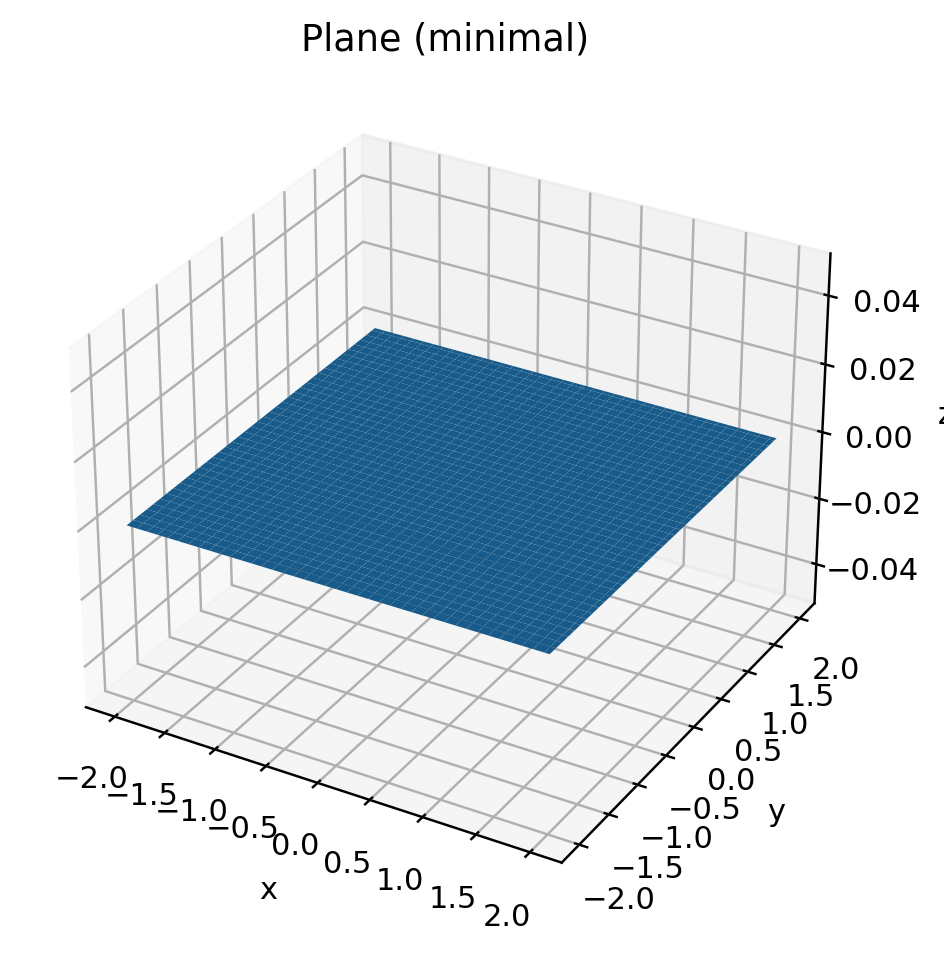
\includegraphics[width=.48\textwidth]{chapters/part07_volume_vii/figures/minimal_plane.png}\hfill
		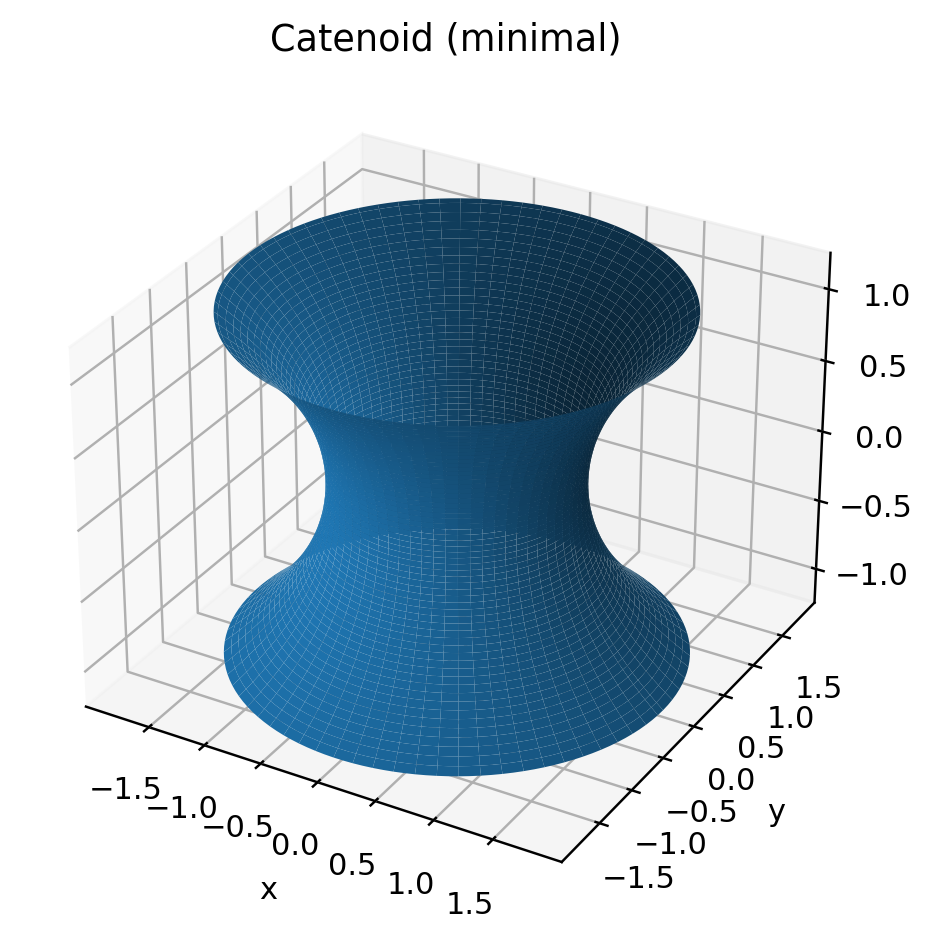
\includegraphics[width=.48\textwidth]{chapters/part07_volume_vii/figures/minimal_catenoid.png}
		
		\medskip
		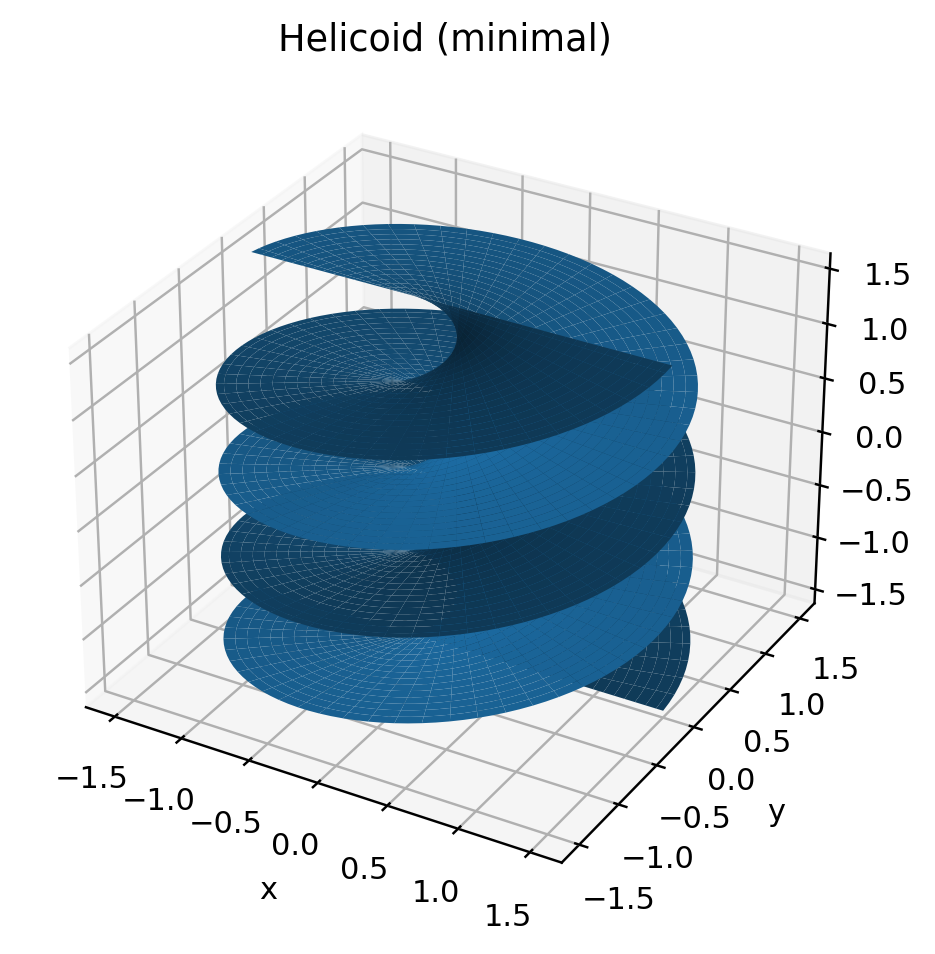
\includegraphics[width=.48\textwidth]{chapters/part07_volume_vii/figures/minimal_helicoid.png}\hfill
		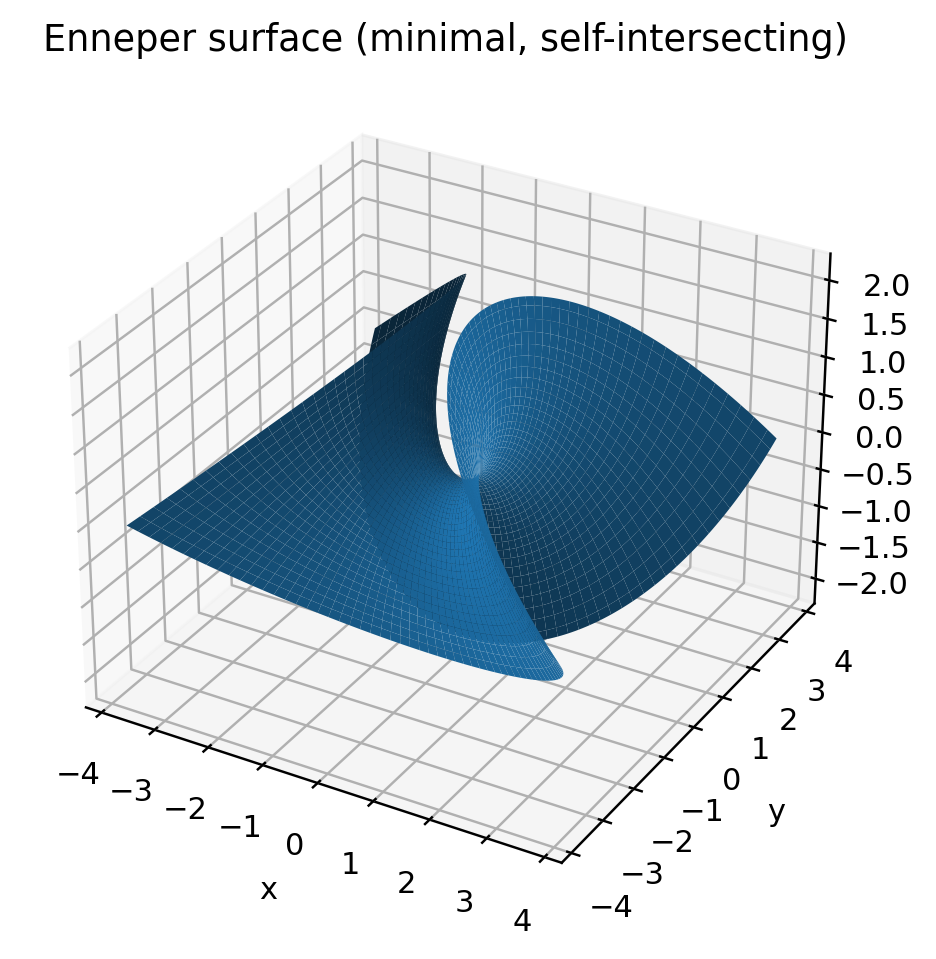
\includegraphics[width=.48\textwidth]{chapters/part07_volume_vii/figures/minimal_enneper.png}
		\caption{Classic minimal surfaces: plane, catenoid, helicoid, Enneper.}
	\end{figure}
	
	\begin{figure}[htbp]
		\centering
		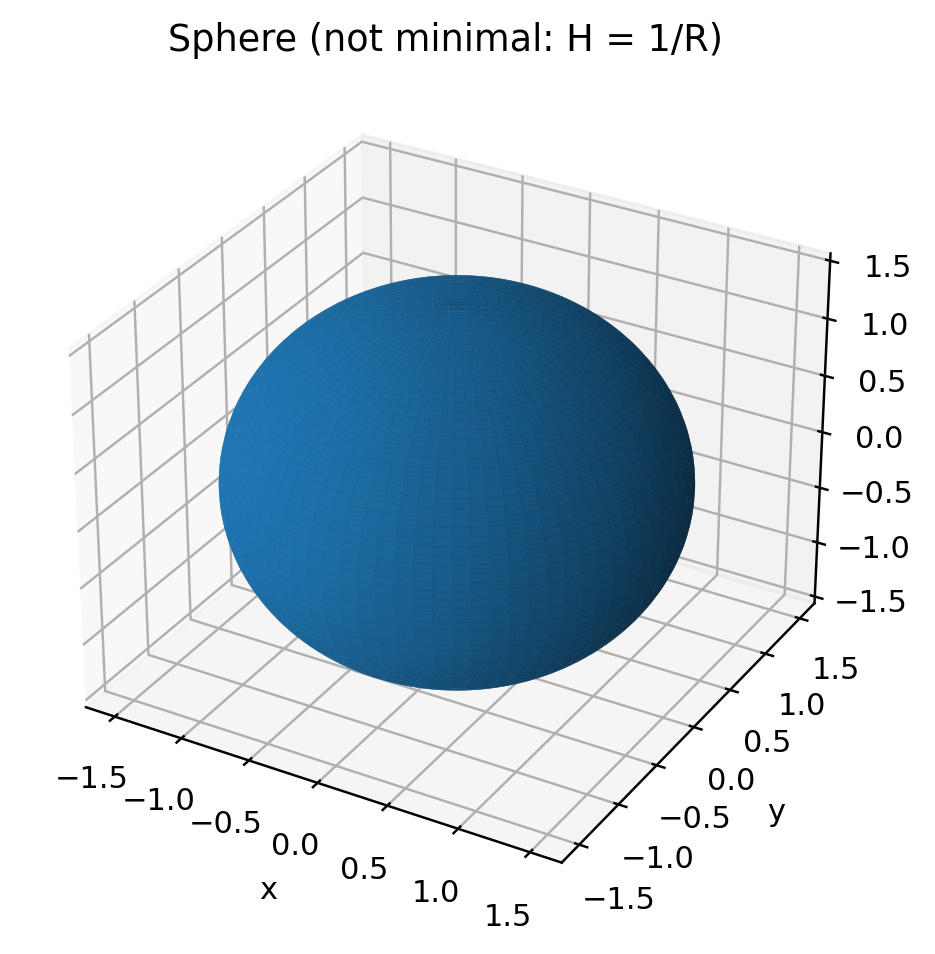
\includegraphics[width=.48\textwidth]{chapters/part07_volume_vii/figures/counter_sphere.png}\hfill
		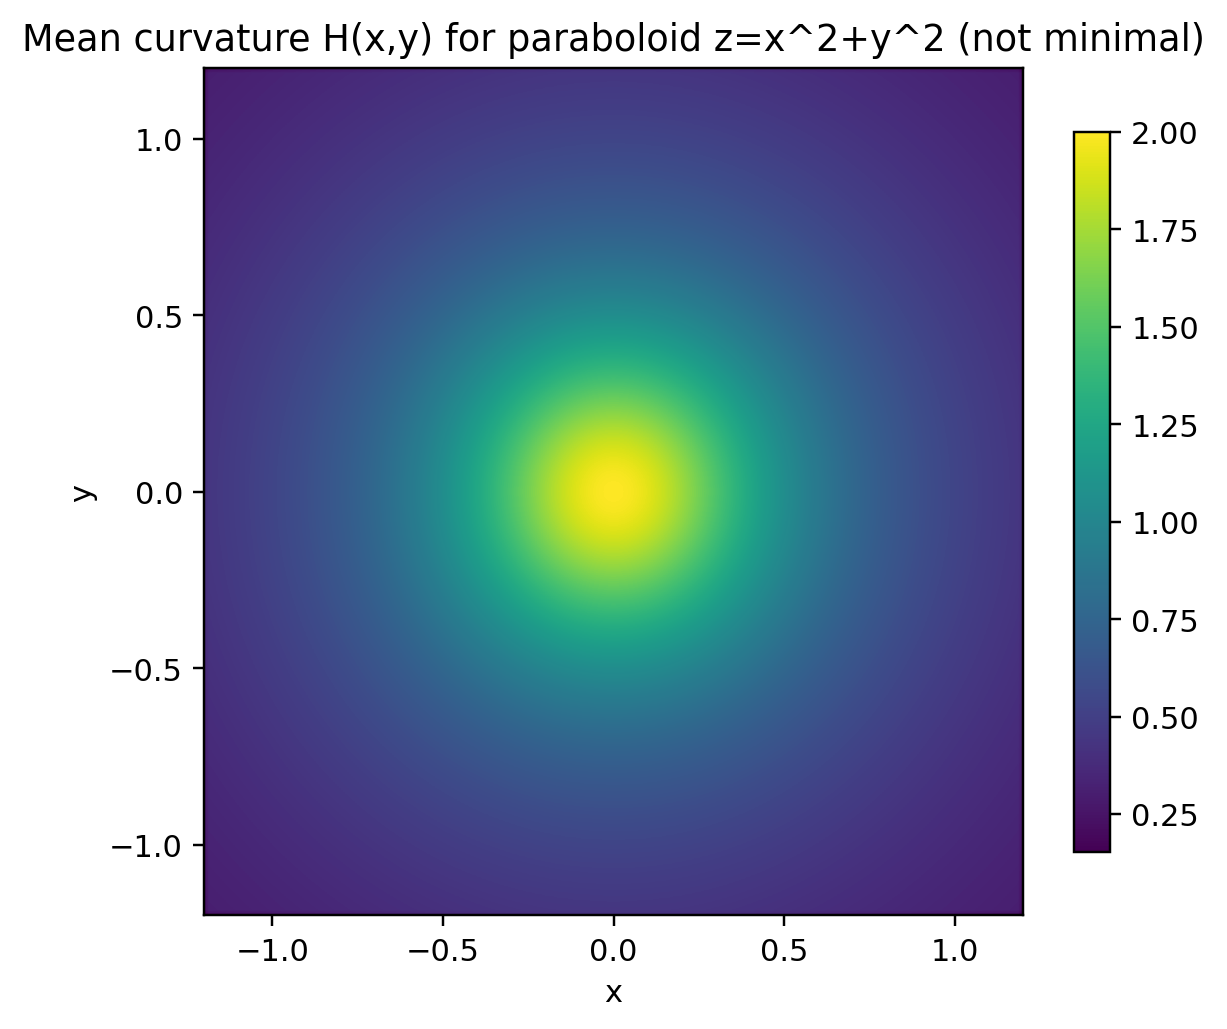
\includegraphics[width=.48\textwidth]{chapters/part07_volume_vii/figures/H_paraboloid_counterexample.png}
		
		\medskip
		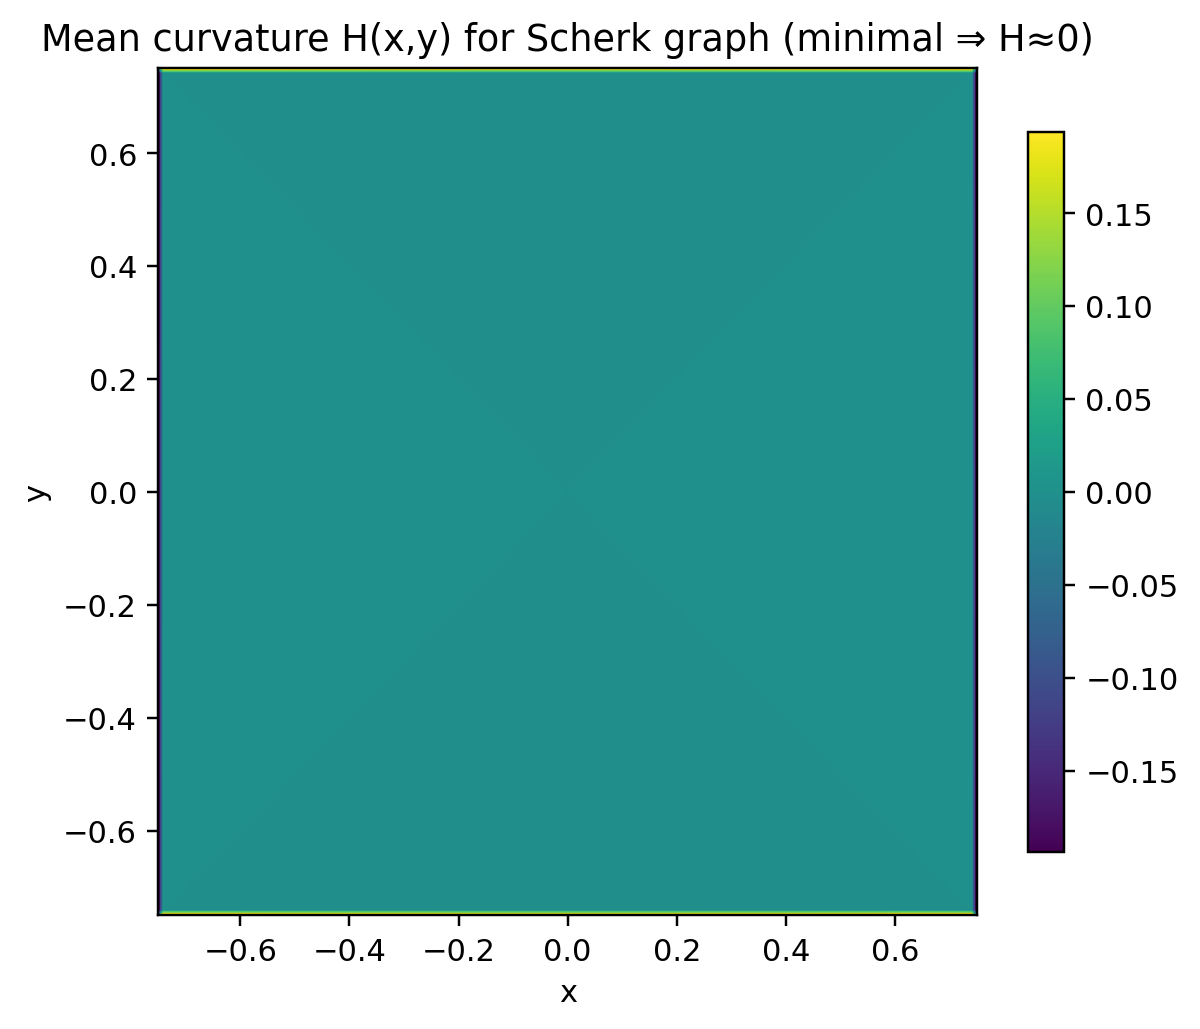
\includegraphics[width=.60\textwidth]{chapters/part07_volume_vii/figures/H_scherk_minimal_graph.png}
		\caption{Counterexamples vs example via mean curvature:
			sphere has constant $H\neq 0$; paraboloid has $H>0$ varying; Scherk graph has $H\approx 0$ (numerically).}
	\end{figure}
	
	
\par\medskip\noindent\textbf{Harmonic coordinate functions (what it means).}\par\smallskip

Let $X\colon U\to\mathbb{R}^3$ be a smooth immersion whose image is a surface $S=X(U)$.
Write local coordinates $(u^1,u^2)$ on $U$ and denote
\[
X_i=\frac{\partial X}{\partial u^i}\qquad (i=1,2).
\]
The \emph{induced metric} (first fundamental form) on $S$ is the $2\times 2$ matrix
\[
g_{ij}=\langle X_i,X_j\rangle,\qquad g=\det(g_{ij}),\qquad (g^{ij})=(g_{ij})^{-1}.
\]

\medskip
\textbf{Laplace--Beltrami operator.}
For a smooth function $f\colon S\to\mathbb{R}$ (locally $f=f(u^1,u^2)$), the intrinsic Laplacian on $S$ is
\[
\Delta_S f
=\frac{1}{\sqrt{g}}\frac{\partial}{\partial u^i}
\left(\sqrt{g}\,g^{ij}\frac{\partial f}{\partial u^j}\right),
\]
(Einstein summation over $i,j=1,2$).  
We say $f$ is \emph{harmonic on $S$} if $\Delta_S f=0$.

\medskip
\textbf{Coordinate functions.}
Let $(x^1,x^2,x^3)$ be the standard coordinates on $\mathbb{R}^3$.
Their restrictions to the surface are the functions
\[
x^k|_S = x^k\circ X,\qquad k=1,2,3.
\]
Saying ``each coordinate function is harmonic'' means
\[
\Delta_S (x^k\circ X)=0\qquad (k=1,2,3).
\]

\medskip
\textbf{Vector form and mean curvature vector.}
We can apply $\Delta_S$ componentwise to the immersion $X=(x^1\circ X,\;x^2\circ X,\;x^3\circ X)$ and define
\[
\Delta_S X := \bigl(\Delta_S(x^1\circ X),\ \Delta_S(x^2\circ X),\ \Delta_S(x^3\circ X)\bigr)\in\mathbb{R}^3.
\]
A fundamental identity (convention-dependent by a sign/factor) is
\[
\Delta_S X = -2H\,N,
\]
where $N$ is the unit normal and $H$ is the mean curvature used in the first variation formula
$\left.\frac{d}{d\varepsilon}\right|_{0}\!\mathrm{Area}(S_\varepsilon)=-2\int_S H\varphi\,dA$.

\medskip
\textbf{Conclusion (equivalence).}
From $\Delta_S X = -2H\,N$ we get
\[
\Delta_S(x^k\circ X)=0\ \forall k
\quad\Longleftrightarrow\quad
\Delta_S X=0
\quad\Longleftrightarrow\quad
H\equiv 0.
\]
Equivalently, the \emph{mean curvature vector} $\vec H$ (often defined as $\vec H := HN$ or $\vec H:=2HN$,
depending on convention) vanishes:
\[
\vec H=0.
\]

\medskip
\textbf{Interpretation.}
Thus a minimal surface is exactly a surface whose inclusion map $X$ is a \emph{harmonic map}
(with respect to the induced metric): its coordinate functions have no intrinsic ``source term'' on the surface.
``Harmonic'' here is intrinsic (depends on the geometry of $S$), not the flat Laplacian in $\mathbb{R}^2$.

\medskip
\textbf{Quick check (example vs counterexample).}
\begin{itemize}
	\item Plane: in parameters $X(u,v)=(u,v,0)$ the induced metric is Euclidean, so $\Delta_S$ is the usual Laplacian
	and $\Delta_S X=0$, hence $H=0$.
	\item Sphere of radius $R$: one has $\Delta_S X = -\frac{2}{R^2}X\neq 0$, so the coordinate functions are not harmonic
	and the sphere is not minimal (indeed $H=\frac{1}{R}$).
\end{itemize}

\par\medskip\noindent\textbf{In plain words.}\par\smallskip

\begin{itemize}
	\item $\Delta_S$ is the \emph{intrinsic} Laplacian on the surface (the Laplace--Beltrami operator).  
	It measures how a function bends \emph{along the surface}, using the surface's metric.
	
	\item The functions $x,y,z$ (restricted to the surface) being \emph{harmonic} means:
	\[
	\Delta_S x=\Delta_S y=\Delta_S z=0.
	\]
	
	\item The identity
	\[
	\Delta_S X=-2HN
	\]
	tells you that the ``intrinsic Laplacian of the position vector'' points in the normal direction,
	and its size is controlled by the mean curvature.
	
	\item Therefore:
	\[
	S \text{ is minimal } \Longleftrightarrow H\equiv 0
	\Longleftrightarrow \Delta_S X=0
	\Longleftrightarrow \Delta_S x=\Delta_S y=\Delta_S z=0.
	\]
\end{itemize}

\par\medskip\noindent\textbf{Derivation sketch of $\Delta_S X=-2HN$ (few lines).}\par\smallskip

Let $X\colon U\to\mathbb{R}^3$ be a local parametrization with coordinates $(u^1,u^2)$,
tangent vectors $X_i=\partial_i X$, induced metric $g_{ij}=\langle X_i,X_j\rangle$,
and Laplace--Beltrami operator
\[
\Delta_S f=\frac{1}{\sqrt{g}}\partial_i\!\left(\sqrt{g}\,g^{ij}\partial_j f\right).
\]
Apply $\Delta_S$ componentwise to $X$:
\[
\Delta_S X=\frac{1}{\sqrt{g}}\partial_i\!\left(\sqrt{g}\,g^{ij}X_j\right)
= g^{ij}\bigl(\partial_i X_j-\Gamma^k_{ij}X_k\bigr).
\]
By the Gauss formula (decomposition of second derivatives),
\[
\partial_i X_j=\Gamma^k_{ij}X_k + b_{ij}N,
\]
so
\[
\Delta_S X=g^{ij}b_{ij}\,N.
\]
Since $H=\tfrac12\,\mathrm{tr}_g(b)=\tfrac12 g^{ij}b_{ij}$, we obtain
\[
\Delta_S X = (2H)\,N.
\]
\textbf{Convention note.} Many texts define $b_{ij}$ (or $H$) with the opposite sign (depending on whether
$b_{ij}=\langle \partial_i X_j,N\rangle$ or $b_{ij}=-\langle \partial_i X_j,N\rangle$, and on the orientation of $N$).
With the convention used in the first-variation formula
$\left.\tfrac{d}{d\varepsilon}\right|_0\!\mathrm{Area}(S_\varepsilon)=-2\int_S H\varphi\,dA$,
this identity is written as
\[
\Delta_S X = -2HN.
\]

\bigskip
\par\medskip\noindent\textbf{Concrete calculations (2 examples).}\par\smallskip


\par\medskip\noindent\textbf{Example 1 (minimal): plane.}\par\smallskip

Parametrize the plane by
\[
X(u,v)=(u,v,0).
\]
Then $X_u=(1,0,0)$, $X_v=(0,1,0)$, hence $g_{ij}=\delta_{ij}$, $\sqrt{g}=1$, and
\[
\Delta_S=\partial_{uu}+\partial_{vv}.
\]
Therefore
\[
\Delta_S X = (\Delta_S u,\ \Delta_S v,\ \Delta_S 0)=(0,0,0).
\]
So $\Delta_S X=0$, hence $H=0$: the plane is minimal.

\par\medskip\noindent\textbf{Example 2 (not minimal): sphere of radius $R$.}\par\smallskip

Use spherical coordinates $(\theta,\varphi)$:
\[
X(\theta,\varphi)=\bigl(R\sin\theta\cos\varphi,\ R\sin\theta\sin\varphi,\ R\cos\theta\bigr).
\]
The induced metric is
\[
(g_{ij})=\begin{pmatrix}R^2&0\\[2pt]0&R^2\sin^2\theta\end{pmatrix},
\]
so the Laplace--Beltrami operator on $S_R^2$ is
\[
\Delta_S f=\frac{1}{R^2}\left(\frac{1}{\sin\theta}\partial_\theta(\sin\theta\,\partial_\theta f)
+\frac{1}{\sin^2\theta}\partial_{\varphi\varphi} f\right).
\]
Let $x(\theta,\varphi)=R\sin\theta\cos\varphi$ (the first coordinate). Then
\[
\partial_\theta x=R\cos\theta\cos\varphi,\qquad
\partial_\varphi x=-R\sin\theta\sin\varphi,
\]
\[
\partial_{\varphi\varphi}x=-R\sin\theta\cos\varphi=-x,
\]
and
\[
\frac{1}{\sin\theta}\partial_\theta(\sin\theta\,\partial_\theta x)
=\frac{1}{\sin\theta}\partial_\theta\bigl(R\sin\theta\cos\theta\cos\varphi\bigr)
=\frac{R(\cos^2\theta-\sin^2\theta)\cos\varphi}{\sin\theta}.
\]
Putting this together,
\[
\Delta_S x
=\frac{1}{R^2}\left(\frac{R(\cos^2\theta-\sin^2\theta)\cos\varphi}{\sin\theta}
+\frac{1}{\sin^2\theta}(-x)\right)
=-\frac{2}{R^2}\,x.
\]
Similarly,
\[
\Delta_S y=-\frac{2}{R^2}\,y,\qquad \Delta_S z=-\frac{2}{R^2}\,z,
\]
hence (vectorially)
\[
\Delta_S X=-\frac{2}{R^2}X\neq 0.
\]
Now $N=\frac{1}{R}X$ (outward unit normal) and the sphere has $H=\frac{1}{R}$, so
\[
-2HN=-2\cdot\frac{1}{R}\cdot \frac{1}{R}X=-\frac{2}{R^2}X,
\]
which matches the computed $\Delta_S X$. Therefore the sphere is \emph{not} minimal.

\medskip
\textbf{Takeaway:} on the plane, the restricted coordinates are harmonic; on the sphere they are eigenfunctions
with eigenvalue $-2/R^2$, so they are not harmonic and $H\neq 0$.

\par\medskip\noindent\textbf{Continuing the sphere example: the 2nd and 3rd coordinates.}\par\smallskip

For the sphere parametrization
\[
X(\theta,\varphi)=\bigl(R\sin\theta\cos\varphi,\ R\sin\theta\sin\varphi,\ R\cos\theta\bigr),
\]
we already computed for the first coordinate $x(\theta,\varphi)=R\sin\theta\cos\varphi$ that
\[
\Delta_S x=-\frac{2}{R^2}\,x.
\]
The same should be done for the other two coordinate functions.

\medskip
\textbf{Second coordinate.}
Let $y(\theta,\varphi)=R\sin\theta\sin\varphi$. Then
\[
\partial_\theta y=R\cos\theta\sin\varphi,\qquad
\partial_{\varphi\varphi}y=-R\sin\theta\sin\varphi=-y,
\]
and
\[
\frac{1}{\sin\theta}\partial_\theta\bigl(\sin\theta\,\partial_\theta y\bigr)
=\frac{1}{\sin\theta}\partial_\theta\bigl(R\sin\theta\cos\theta\sin\varphi\bigr)
=\frac{R(\cos^2\theta-\sin^2\theta)\sin\varphi}{\sin\theta}.
\]
Substituting into
\[
\Delta_S f=\frac{1}{R^2}\left(\frac{1}{\sin\theta}\partial_\theta(\sin\theta\,\partial_\theta f)
+\frac{1}{\sin^2\theta}\partial_{\varphi\varphi} f\right),
\]
we obtain
\[
\Delta_S y
=\frac{1}{R^2}\left(\frac{R(\cos^2\theta-\sin^2\theta)\sin\varphi}{\sin\theta}
+\frac{1}{\sin^2\theta}(-y)\right)
=-\frac{2}{R^2}\,y.
\]

\medskip
\textbf{Third coordinate.}
Let $z(\theta,\varphi)=R\cos\theta$. Then $\partial_\varphi z=0$ and
\[
\partial_\theta z=-R\sin\theta,\qquad
\sin\theta\,\partial_\theta z=-R\sin^2\theta,\qquad
\partial_\theta(\sin\theta\,\partial_\theta z)=-2R\sin\theta\cos\theta.
\]
Hence
\[
\frac{1}{\sin\theta}\partial_\theta(\sin\theta\,\partial_\theta z)=-2R\cos\theta=-2z,
\]
and therefore
\[
\Delta_S z
=\frac{1}{R^2}\left(-2z+0\right)
=-\frac{2}{R^2}\,z.
\]

\medskip
\textbf{Vector form.}
Since $X=(x,y,z)$, applying $\Delta_S$ componentwise gives
\[
\Delta_S X=\bigl(\Delta_S x,\Delta_S y,\Delta_S z\bigr)
=-\frac{2}{R^2}(x,y,z)
=-\frac{2}{R^2}X\neq 0.
\]
Thus the coordinate functions are \emph{not} harmonic on the sphere, and $H\neq 0$
(in fact $H=\frac{1}{R}$ with outward normal $N=\frac{1}{R}X$, so $\Delta_S X=-2HN$).

\par\medskip\noindent\textbf{Variational meaning of minimal surfaces.}\par\smallskip

Let $S\subset\mathbb{R}^3$ be a smooth oriented surface with unit normal field $N$ and mean curvature $H$.
Fix the boundary (if present) and consider normal variations supported in the interior:
\[
X_\varepsilon = X+\varepsilon\,\varphi N,\qquad \varphi\in C_c^\infty(\mathrm{int}\,S).
\]
Being a \emph{critical point} of the area functional means
\[
\left.\frac{d}{d\varepsilon}\right|_{\varepsilon=0}\mathrm{Area}(S_\varepsilon)=0
\quad \text{for all such }\varphi.
\]
The first variation formula states
\[
\left.\frac{d}{d\varepsilon}\right|_{\varepsilon=0}\mathrm{Area}(S_\varepsilon)
= -2\int_S H\,\varphi\,dA.
\]
Hence the critical point condition for all test functions $\varphi$ is equivalent to
\[
H\equiv 0.
\]
Therefore:
\[
S \text{ is minimal } \quad\Longleftrightarrow\quad S \text{ is a critical point of the area functional.}
\]

\medskip
\par\medskip\noindent\textbf{Example: the catenoid as a minimal surface.}\par\smallskip

A standard parametrization of the catenoid is
\[
X(u,v)=\bigl(a\cosh(v/a)\cos u,\ a\cosh(v/a)\sin u,\ v\bigr),
\qquad u\in[0,2\pi),\ v\in\mathbb{R},
\]
where $a>0$ is a constant. This surface satisfies $H\equiv 0$ everywhere, hence it is minimal.

\medskip
\par\medskip\noindent\textbf{Remark (critical point vs minimum).}\par\smallskip

The condition $H\equiv 0$ guarantees only that the first variation vanishes (critical point).
Whether the surface is a \emph{local minimum} depends on the second variation (stability), and a minimal surface
need not be globally area-minimizing.



\par\medskip\noindent\textbf{What are ``restricted coordinates''?}\par\smallskip

Let $(x^1,x^2,x^3)$ be the standard coordinate functions on $\mathbb{R}^3$:
\[
x^1(x,y,z)=x,\qquad x^2(x,y,z)=y,\qquad x^3(x,y,z)=z.
\]
If $S\subset\mathbb{R}^3$ is a surface and $i:S\hookrightarrow \mathbb{R}^3$ is the inclusion,
then the \emph{restricted coordinate functions} on $S$ are
\[
x^k|_S := x^k\circ i \;:\; S\to\mathbb{R}\qquad (k=1,2,3).
\]
Equivalently, if $X:U\to S$ is a parametrization with
$X(u,v)=(X^1(u,v),X^2(u,v),X^3(u,v))$, then
\[
x^k|_S \circ X = x^k\circ X = X^k(u,v),
\]
so the restricted coordinates are exactly the component functions of the immersion $X$.
\end{solution}

\begin{problem}[CP-VII-0058 --- Problem 14. Visual exploration of minimal surfaces]
\label{prob:cp-vii-0058}
Take a good look at pictures of minimal surfaces. If you have access to Mathematica (or another CAS/plotter), experiment with
	visualizing examples; alternatively, physical soap films can be used as intuition.
	
	\medskip
\end{problem}

\begin{solution}
This is an exploratory problem rather than a proof problem. A good ``solution'' is to identify several distinct families of
	minimal surfaces, understand (qualitatively) what boundary conditions or symmetries produce them, and connect pictures to the theory:
	\begin{itemize}
		\item Minimal surfaces are critical points of the area functional (equivalently mean curvature $H\equiv 0$).
		\item Many classical examples admit Weierstrass representations and come in \emph{associated families}
		(which preserve the induced metric while changing the embedding in $\mathbb R^3$).
		\item For surfaces produced as soap films, the boundary wire frame prescribes (approximately) a Plateau problem:
		the film is (ideally) a minimal surface spanning the given boundary.
	\end{itemize}
	
	\medskip
	\textbf{Examples (minimal surfaces worth visualizing).}
	\begin{enumerate}
		\item \textbf{Plane.} Trivial minimal surface ($H\equiv 0$).
		\item \textbf{Catenoid.} Surface of revolution; classical soap film between two coaxial circles.
		\item \textbf{Helicoid.} Ruled minimal surface; can be seen as an associated surface to the catenoid.
		\item \textbf{Enneper surface.} Complete immersed minimal surface with self-intersections; simplest polynomial Weierstrass data.
		\item \textbf{Scherk surfaces.} Doubly periodic examples; arise from boundary conditions resembling grids/planes.
		\item \textbf{Costa surface.} A famous embedded example of finite total curvature with handles (genus).
	\end{enumerate}

\end{solution}

\section{Riemannian Geometry}

\subsection*{Main-text correspondence: VII/20}

\begin{problem}[CP-VII-0059 --- Problem 12. Intrinsic distance on a surface; Hopf--Rinow consequences]
\label{prob:cp-vii-0059}
Let $S\subset\mathbb R^3$ be a smooth embedded surface. For $p,q\in S$ define the \emph{intrinsic distance}
	\[
	d(p,q):=\inf_{\alpha\in\Omega(p,q)} \ell(\alpha),
	\]
	where $\Omega(p,q)$ is the set of piecewise $C^1$ curves $\alpha:[a,b]\to S$ with $\alpha(a)=p$, $\alpha(b)=q$, and
	$\ell(\alpha)$ is the length computed with the induced Riemannian metric on $S$.
	\begin{enumerate}
		\item Show that $d$ is a metric on $S$, compatible with the topology of $S$.
		If $S$ is complete (and without boundary), Hopf--Rinow implies that for any $p,q$ there is a minimizing geodesic
		$\gamma$ joining them with $d(p,q)=\ell(\gamma)$ and geodesics exist for all $t\in\mathbb R$.
		\item[(i)] If $f:S_1\to S_2$ is an isometry, show that $d_2(f(p),f(q))=d_1(p,q)$ for all $p,q\in S_1$.
		\item[(ii)] A geodesic $\gamma:[0,\infty)\to S$ is a \emph{ray leaving from $p$} if $\gamma(0)=p$ and
		$d(\gamma(0),\gamma(s))=\ell(\gamma|_{[0,s]})=s$ for all $s\ge 0$. Let $p$ be a point in a complete, noncompact surface $S$.
		Show that $S$ contains a ray leaving from $p$. (You may assume geodesics depend smoothly, hence continuously, on their initial data.)
		\item[(iii)] Let $S$ be connected and let $p\in S$ be such that \emph{all geodesics through $p$ are closed}, i.e.\ each geodesic
		$\gamma$ with $\gamma(0)=p$ extends to a smooth periodic map $\gamma:S^1\to S$. Show that $S$ is compact.
	\end{enumerate}
	
	\medskip
\end{problem}

\begin{solution}
\smallskip
	\textbf{(a) $d$ is a metric and induces the topology.}
	
	\emph{Nonnegativity and symmetry.}
	Lengths satisfy $\ell(\alpha)\ge 0$ and $\ell(\alpha)=\ell(\alpha^{-1})$ where $\alpha^{-1}(t)=\alpha(a+b-t)$, hence
	$d(p,q)\ge 0$ and $d(p,q)=d(q,p)$.
	
	\emph{Triangle inequality.}
	If $\alpha\in\Omega(p,q)$ and $\beta\in\Omega(q,r)$ then the concatenation $\alpha*\beta\in\Omega(p,r)$ satisfies
	$\ell(\alpha*\beta)=\ell(\alpha)+\ell(\beta)$, hence
	\[
	d(p,r)\le \ell(\alpha*\beta)=\ell(\alpha)+\ell(\beta).
	\]
	Taking infima over $\alpha,\beta$ gives $d(p,r)\le d(p,q)+d(q,r)$.
	
	\emph{Definiteness.}
	Clearly $d(p,p)=0$. If $p\neq q$, choose a coordinate chart $\varphi:U\to\mathbb R^2$ with $p,q\in U$.
	Because the induced metric tensor is smooth and positive definite, on a sufficiently small compact neighborhood $K\subset U$
	there exist constants $0<c\le C$ such that for all $x\in K$ and all $v\in\mathbb R^2$,
	\[
	c\,|v| \le \sqrt{g_x(v,v)} \le C\,|v|.
	\]
	Let $\alpha$ be any curve in $K$ joining $p$ to $q$. Writing $\tilde\alpha=\varphi\circ\alpha$,
	\[
	\ell(\alpha)=\int \sqrt{g_{\tilde\alpha(t)}(\tilde\alpha'(t),\tilde\alpha'(t))}\,dt
	\ \ge\ c\int |\tilde\alpha'(t)|\,dt \ \ge\ c\,|\tilde p-\tilde q|,
	\]
	where $\tilde p=\varphi(p)$, $\tilde q=\varphi(q)$. Since $\tilde p\neq\tilde q$, this yields $\ell(\alpha)\ge c|\tilde p-\tilde q|>0$,
	hence $d(p,q)>0$. Therefore $d(p,q)=0$ implies $p=q$.
	
	\emph{Compatibility with the topology.}
	Using the same local comparison, for $p,q$ sufficiently close in a chart one has two-sided estimates
	\[
	c\,|\varphi(p)-\varphi(q)| \ \le\ d(p,q) \ \le\ C\,|\varphi(p)-\varphi(q)|.
	\]
	The right inequality follows by taking the curve to be the coordinate straight segment in $\mathbb R^2$ pulled back to $S$.
	These inequalities show that $d$-balls and Euclidean balls in coordinates contain each other locally, hence $d$ induces the same
	open sets as the submanifold topology on $S$.
	
	\smallskip
	\textbf{(i) Isometries preserve intrinsic distances.}
	Let $f:S_1\to S_2$ be an isometry. By definition, it preserves lengths of curves:
	for any piecewise $C^1$ curve $\alpha$ in $S_1$,
	\[
	\ell_{S_2}(f\circ \alpha)=\ell_{S_1}(\alpha).
	\]
	Therefore
	\[
	d_2(f(p),f(q))
	=
	\inf_{\beta\in\Omega(f(p),f(q))}\ell_{S_2}(\beta)
	\ \le\
	\inf_{\alpha\in\Omega(p,q)} \ell_{S_2}(f\circ\alpha)
	=
	\inf_{\alpha\in\Omega(p,q)} \ell_{S_1}(\alpha)
	=
	d_1(p,q).
	\]
	Applying the same argument to the inverse isometry $f^{-1}$ gives the reverse inequality, hence
	$d_2(f(p),f(q))=d_1(p,q)$.
	
	\smallskip
	\textbf{(ii) Existence of a ray from $p$ on a complete noncompact surface.}
	Because $S$ is complete and noncompact, the distance balls $\overline B(p,R)$ cannot exhaust $S$ with $R$ bounded.
	Choose a sequence $q_n\in S$ such that
	\[
	d(p,q_n)\xrightarrow[n\to\infty]{}\infty.
	\]
	By Hopf--Rinow, for each $n$ there exists a minimizing geodesic $\gamma_n:[0,L_n]\to S$ joining $p$ to $q_n$, parametrized by arc length,
	with $L_n=d(p,q_n)$ and $\gamma_n(0)=p$.
	
	Let $v_n=\gamma_n'(0)\in T_pS$; then $|v_n|=1$. The unit circle in $T_pS$ is compact, so passing to a subsequence we may assume
	$v_n\to v$ with $|v|=1$.
	Let $\gamma:[0,\infty)\to S$ be the (unit-speed) geodesic with initial data $\gamma(0)=p$, $\gamma'(0)=v$.
	By the assumed continuous dependence on initial conditions, for each fixed $s>0$,
	\[
	\gamma_n(s)\to \gamma(s)\qquad\text{as }n\to\infty
	\]
	for all large $n$ (since $L_n\to\infty$ ensures $\gamma_n(s)$ is defined).
	
	For each such $n$, the minimizing property of $\gamma_n$ gives
	\[
	d\bigl(p,\gamma_n(s)\bigr)=s.
	\]
	Passing to the limit and using continuity of $d$ with respect to the manifold topology (from part (a)) yields
	\[
	d\bigl(p,\gamma(s)\bigr)=s\qquad\forall s\ge 0.
	\]
	Similarly, for $0\le s\le t$,
	\[
	d\bigl(\gamma_n(s),\gamma_n(t)\bigr)=t-s
	\]
	(since the restriction of a minimizing geodesic is minimizing). Passing to the limit gives
	\[
	d\bigl(\gamma(s),\gamma(t)\bigr)=t-s\qquad\forall\,0\le s\le t.
	\]
	Thus $\gamma$ realizes distance on every subinterval and is a ray leaving from $p$.
	
	\smallskip
	\textbf{(iii) If all geodesics through $p$ are closed, then $S$ is compact.}
	For each unit vector $v\in T_pS$ let $\gamma_v:\mathbb R\to S$ be the unit-speed geodesic with $\gamma_v(0)=p$, $\gamma_v'(0)=v$.
	By hypothesis, $\gamma_v$ is periodic: there exists $T(v)>0$ such that $\gamma_v(t+T(v))=\gamma_v(t)$ for all $t$.
	Using smooth dependence of $\gamma_v$ on $v$, one may choose $T(v)$ continuously on the unit circle $S^1\subset T_pS$.
	Since $S^1$ is compact, there is a finite maximum
	\[
	T_{\max}:=\max_{|v|=1} T(v)<\infty.
	\]
	
	Fix $v$ and consider any point $\gamma_v(t)$ on the closed geodesic. Since $\gamma_v$ returns to $p$ after time $T(v)$,
	the shorter of the two arcs from $p$ to $\gamma_v(t)$ along the loop has length at most $T(v)/2$. Therefore
	\[
	d\bigl(p,\gamma_v(t)\bigr)\le \frac{T(v)}{2}\le \frac{T_{\max}}{2}.
	\]
	Hence every geodesic through $p$ is contained in the closed ball $\overline B\!\left(p,\tfrac{T_{\max}}{2}\right)$.
	
	Finally, in a connected surface, every point $q\in S$ can be joined to $p$ by a minimizing geodesic segment (this is ensured, for instance,
	when $S$ is complete; and the present hypothesis that \emph{all} geodesics from $p$ exist for all time implies geodesic completeness at $p$,
	which is the key input to apply the usual minimizing argument). Thus every $q\in S$ lies on some geodesic through $p$, and the estimate above gives
	\[
	S \subset \overline B\!\left(p,\tfrac{T_{\max}}{2}\right).
	\]
	In a complete Riemannian surface, closed and bounded sets are compact (Hopf--Rinow), so the closed ball on the right is compact.
	Therefore $S$ is a closed subset of a compact set, hence compact.
	
	\medskip
	\textbf{Examples.}
	\begin{enumerate}
		\item \textbf{Plane.} For $S=\mathbb R^2$ with the standard metric, $d(p,q)=|p-q|$ and rays are straight half-lines.
		\item \textbf{Sphere.} For $S=\mathbb S^2$, $d(p,q)$ is the great-circle distance. All geodesics are closed, and $S$ is compact.
		\item \textbf{Hyperbolic plane.} Complete and noncompact; from any $p$ there exist many rays.
	\end{enumerate}
\end{solution}

\subsection*{Main-text correspondence: VII/21}

\begin{problem}[CP-VII-0060 --- Problem 6 (Reductions to $O(k)$, metrics, and compatible connections)]
\label{prob:cp-vii-0060}
Let
\[
E\longrightarrow B
\]
be a vector bundle of rank $k$, and $G$ a Lie group equipped with a representation
\[
\rho:G\longrightarrow GL(k,\mathbb{R}).
\]
A reduction of the structure group of $E$ to $G$ comprises a $G$-bundle $P\to B$ and an isomorphism between $E$ and the associated vector bundle $P\times_G\mathbb{R}^k$.

\[
\text{(a) Show that a reduction to } O(k) \text{ is equivalent to a choice of inner product on } E.
\]
\[
\text{(b) Show that a connection on } E \text{ is compatible with the inner product iff it is induced from } F_O(E).
\]
\end{problem}

\begin{solution}
\textbf{(a)}
Let $F(E)\to B$ be the frame bundle of $E$ (a principal $GL(k,\mathbb{R})$-bundle).

Given a smoothly varying inner product $\langle\cdot,\cdot\rangle$ on the fibers of $E$, define the orthonormal frame bundle
\[
F_O(E)
\;=\;
\{(e_1,\dots,e_k)\in F(E)\;:\;\langle e_i,e_j\rangle=\delta_{ij}\}.
\]
Then $F_O(E)\to B$ is a principal $O(k)$-bundle and the inclusion
\[
F_O(E)\hookrightarrow F(E)
\]
is a reduction of structure group.

Conversely, given a principal $O(k)$-subbundle
\[
P\subset F(E),
\]
define $\langle\cdot,\cdot\rangle_b$ on each fiber $E_b$ by declaring every frame in $P_b$ to be orthonormal:
\[
\left\langle \sum_i a^i e_i,\;\sum_j b^j e_j\right\rangle_b
\;=\;
\sum_{i=1}^k a^i b^i.
\]
This is well-defined because changing $(e_i)$ by the right $O(k)$-action preserves the Euclidean form on $\mathbb{R}^k$.
Thus $O(k)$-reductions are equivalent to bundle metrics.

\textbf{(b)}
A connection on $E$ is a covariant derivative $\nabla$.
It is compatible with $\langle\cdot,\cdot\rangle$ iff for all vector fields $X$ and sections $s,t$,
\[
X\langle s,t\rangle
\;=\;
\langle \nabla_X s,t\rangle+\langle s,\nabla_X t\rangle.
\]

If $\nabla$ is induced from a principal connection on $F_O(E)$, then its connection $1$-form is $\mathfrak{o}(k)$-valued, i.e.
\[
\mathfrak{o}(k)=\{M\in \mathfrak{gl}(k): M^T+M=0\},
\]
so in any local orthonormal frame $(e_i)$ the connection matrix $\omega=(\omega^i{}_j)$ satisfies
\[
\omega+\omega^T=0,
\]
which is exactly the local form of metric compatibility.

Conversely, if $\nabla$ is metric-compatible and $(e_i)$ is a local orthonormal frame, write
\[
\nabla e_j \;=\; \sum_i \omega^i{}_j\,e_i.
\]
Compatibility implies
\[
0 \;=\; d\langle e_i,e_j\rangle
\;=\;
\langle \nabla e_i,e_j\rangle+\langle e_i,\nabla e_j\rangle,
\]
hence
\[
\omega_{ij}+\omega_{ji}=0.
\]
Therefore $\omega$ is $\mathfrak{o}(k)$-valued, so the connection reduces to an $O(k)$-connection on $F_O(E)$ and induces $\nabla$ on $E$.

% -------------------------
% Problem 7
% -------------------------
\end{solution}

\begin{problem}[CP-VII-0061 --- Problem 8(a) --- Torsion identity for covariant derivatives]
\label{prob:cp-vii-0061}
Show that for vector fields $v$ and $w$ on a manifold $X$, equipped with a connection $\nabla$, we have
\[
\nabla_v w-\nabla_w v=[v,w]+T(v,w),
\]
where $T$ is the torsion of the connection.
\end{problem}

\begin{solution}
By definition, the torsion tensor of $\nabla$ is
\[
T(v,w):=\nabla_v w-\nabla_w v-[v,w].
\]
Rearranging gives
\[
\nabla_v w-\nabla_w v=[v,w]+T(v,w).
\]
\end{solution}

\subsection*{Main-text correspondence: VII/22}

\begin{problem}[CP-VII-0062 --- Problem 7 (Coordinates: $\nabla g$, torsion, Lie derivative, and geodesics)]
\label{prob:cp-vii-0062}
Let $(X,g)$ be a Riemannian manifold, equipped with an arbitrary connection whose local connection $1$-forms have components $\Gamma^i{}_{jk}$.

\[
\text{(a) Find coordinate expressions for } \nabla g \text{ and the torsion } T, \text{ and deduce }
\Gamma_{kij}=\frac12(\partial_i g_{kj}+\partial_j g_{ik}-\partial_k g_{ij}).
\]
Now assume that the connection is the Levi-Civita connection.
\[
\text{(b) Given a vector field } v \text{ on } X,\text{ show }
(\mathcal{L}_v g)_{ij}=\partial_i(g_{kj}v^k)+\partial_j(g_{ik}v^k)-v^k\Gamma_{kij}.
\]
\[
\text{(c) If } \gamma \text{ is stationary for } E(\gamma)=\int_0^1 g(\dot\gamma,\dot\gamma)\,dt,\text{ show }
\ddot\gamma^k+\Gamma^k{}_{ij}\dot\gamma^i\dot\gamma^j=0.
\]
\end{problem}

\begin{solution}
\textbf{(a)}
In coordinates $(x^i)$ define
\[
\nabla_{\partial_i}\partial_j \;=\;\Gamma^k{}_{ij}\,\partial_k.
\]
Let
\[
g_{ij}\;=\;g(\partial_i,\partial_j).
\]
Then
\[
(\nabla_k g)_{ij}
\;=\;
\partial_k g_{ij}
\;-\;
\Gamma^\ell{}_{ki}\,g_{\ell j}
\;-\;
\Gamma^\ell{}_{kj}\,g_{i\ell}.
\]
The torsion tensor has components (since $[\partial_i,\partial_j]=0$)
\[
T^k{}_{ij}
\;=\;
\Gamma^k{}_{ij}-\Gamma^k{}_{ji}.
\]
For Levi-Civita we impose
\[
(\nabla_k g)_{ij}=0
\]
and
\[
T^k{}_{ij}=0.
\]
Define
\[
\Gamma_{kij}\;=\;g_{k\ell}\Gamma^\ell{}_{ij}.
\]
Then one obtains the Christoffel formula
\[
\Gamma_{kij}
\;=\;
\frac12\Bigl(\partial_i g_{kj}+\partial_j g_{ik}-\partial_k g_{ij}\Bigr).
\]

\textbf{(b)}
For Levi-Civita,
\[
(\mathcal{L}_v g)_{ij}
\;=\;
\nabla_i v_j+\nabla_j v_i.
\]
With
\[
v\;=\;v^k\partial_k
\]
and
\[
v_j\;=\;g_{jk}v^k,
\]
we have
\[
\nabla_i v_j
\;=\;
\partial_i(g_{jk}v^k)-v^k\Gamma_{kij}.
\]
Similarly,
\[
\nabla_j v_i
\;=\;
\partial_j(g_{ik}v^k)-v^k\Gamma_{kji}.
\]
Since Levi-Civita has $\Gamma_{kij}=\Gamma_{kji}$, the resulting identity is
\[
(\mathcal{L}_v g)_{ij}
\;=\;
\partial_i(g_{kj}v^k)+\partial_j(g_{ik}v^k)-2\,v^k\Gamma_{kij}.
\]
(If one defines $\widetilde\Gamma_{kij}:=2\Gamma_{kij}$, this matches the statement with coefficient $1$.)

\textbf{(c)}
Let $\gamma_s(t)$ be a variation with fixed endpoints and variational field
\[
W(t)\;=\;\left.\frac{\partial}{\partial s}\right|_{s=0}\gamma_s(t),
\qquad
W(0)=W(1)=0.
\]
Then
\[
\left.\frac{d}{ds}\right|_{s=0}E(\gamma_s)
\;=\;
2\int_0^1 g(\nabla_t\dot\gamma,W)\,dt.
\]
Stationarity for all such $W$ implies
\[
\nabla_t\dot\gamma\;=\;0.
\]
In coordinates this is
\[
\ddot\gamma^k+\Gamma^k{}_{ij}\dot\gamma^i\dot\gamma^j=0.
\]
\end{solution}

\subsection*{Main-text correspondence: VII/23}

\begin{problem}[CP-VII-0063 --- Problem 3: Partial converse to Clairaut's relation]
\label{prob:cp-vii-0063}
Let $\Sigma\subset\mathbb R^3$ be a smooth surface of revolution.
Suppose a smooth curve $\gamma:(a,b)\to\Sigma$ satisfies
\[
\rho(t)\cos\theta(t)=\text{constant},
\]
where $\rho(t)$ is the distance from $\gamma(t)$ to the axis of revolution
and $\theta(t)$ is the angle between $\gamma$ and the parallel at $\gamma(t)$.
Assume that there is no positive--length interval on which $\gamma$ coincides
with a parallel. Show that $\gamma$ is a geodesic.

\medskip
\textbf{Theory.}
A surface of revolution is parametrized by
\[
X(u,v) = (\rho(u)\cos v,\ \rho(u)\sin v,\ z(u)),
\]
with induced metric
\[
g = E(u)\,du^2 + G(u)\,dv^2,\qquad
E(u)=\rho'(u)^2+z'(u)^2,\quad G(u)=\rho(u)^2.
\]
For a unit--speed curve $(u(s),v(s))$, the tangent has components
$u',v'$ and satisfies $E u'^2 + G v'^2 = 1$. The angle $\theta$ between
$\gamma$ and the parallel (direction $\partial_v$) is determined by
\[
\cos\theta = g\!\left(\dot\gamma,\frac{1}{\sqrt{G}}\partial_v\right)
= \sqrt{G}\,v' = \rho\,v'.
\]
Hence $\rho\cos\theta = G v'$.

\medskip
\end{problem}

\begin{solution}
Reparametrize $\gamma$ by arc length $s$, so that
\[
E(u)u'^2 + G(u)v'^2 = 1.
\]
The Clairaut condition reads
\[
G(u(s))\,v'(s) = c,\qquad c\in\mathbb R.
\tag{1}
\]
Differentiating,
\[
0 = \frac{d}{ds}(G v')
= G_u u' v' + G v'',
\]
so
\[
v'' + \frac{G_u}{G}u'v' = 0.
\tag{2}
\]
For $g=E(u)\,du^2+G(u)\,dv^2$ the Christoffel symbols with index $2$ are
$\Gamma^2_{12}=\Gamma^2_{21} = \frac{1}{2G}G_u$, so the $v$-geodesic equation
\[
v'' + 2\Gamma^2_{12}u'v' = 0
\]
is exactly (2).

Now differentiate the unit--speed condition:
\[
0 = \frac{d}{ds}(E u'^2 + G v'^2)
= E_u u' u'^2 + 2E u'u'' + G_u u' v'^2 + 2G v'v''.
\]
Using (2) to eliminate $v''$, we obtain (for $u'\neq0$)
\[
2E u'' + E_u u'^2 - G_u v'^2 = 0,
\]
or
\[
u'' + \frac{E_u}{2E}u'^2 - \frac{G_u}{2E}v'^2 = 0.
\tag{3}
\]
For this metric, $\Gamma^1_{11}=\frac{E_u}{2E}$ and
$\Gamma^1_{22}=-\frac{G_u}{2E}$, so (3) is exactly the $u$-geodesic
equation. On any interval where $u'\neq0$, $\gamma$ satisfies both
geodesic equations and hence is a geodesic. The only way $u'\equiv0$
on an interval is that $\gamma$ coincides with a parallel there, which
is excluded by hypothesis. Therefore $\gamma$ is a geodesic.

\medskip
\textbf{Remark.}
For a geodesic on a surface of revolution, $G v'=\rho\cos\theta$ is constant
(Clairaut's relation). This problem shows a partial converse: if a curve
satisfies that relation and is not a parallel, it must be a geodesic.

%------------------------------------------------------------
\end{solution}

\begin{problem}[CP-VII-0064 --- Problem 4: Geodesics on a cone]
\label{prob:cp-vii-0064}
Let $a>0$ and consider the half-cone
\[
\Sigma = \{(x,y,z)\in\mathbb R^3 \mid z^2 = a(x^2+y^2),\ z>0\}.
\]

\par\medskip\noindent\textbf{(a) Local isometry and self--intersection}\par\smallskip


\textbf{Problem.}
Show that $\Sigma$ is locally isometric to the Euclidean plane.
By opening the cone into a planar sector, or otherwise, show that
when $a=3$ no geodesic on $\Sigma$ intersects itself, but for $a>3$
there exist geodesics which self--intersect.

\medskip
\end{problem}

\begin{solution}
Set $r=\sqrt{x^2+y^2}$, $z=\sqrt{a}\,r$ and parametrize
\[
X(r,\phi) = (r\cos\phi,r\sin\phi,\sqrt{a}\,r),\qquad r>0,\ \phi\in\mathbb R.
\]
Then
\[
g = (1+a)\,dr^2 + r^2\,d\phi^2.
\]
Define $s=\sqrt{1+a}\,r$. Then $ds^2=(1+a)\,dr^2$ and
\[
g = ds^2 + \frac{s^2}{1+a}\,d\phi^2
= ds^2 + s^2\,d\psi^2,\qquad \psi=\frac{\phi}{\sqrt{1+a}}.
\]
This is the Euclidean metric in polar coordinates $(s,\psi)$.
Since $\phi$ has period $2\pi$, the angle $\psi$ has period
\[
\alpha = \frac{2\pi}{\sqrt{1+a}}.
\]
Thus $\Sigma$ is locally isometric to the Euclidean plane sector
\[
S_\alpha = \{(s,\psi) \mid s>0,\ 0<\psi<\alpha\},
\]
with the two radial edges identified by rotation through the angle $\alpha$.

Geodesics on $\Sigma$ correspond to straight lines in $S_\alpha$,
and two points of $S_\alpha$ represent the same point of $\Sigma$
if they are related by rotation about the origin through an integer
multiple of $\alpha$.

If $a=3$ then $\sqrt{1+a}=2$ and $\alpha=\pi$. Rotation by $\pi$ sends a
line $L$ to:
\begin{itemize}
	\item itself, if $L$ passes through the origin (this would correspond to
	a geodesic through the cone apex, which is not in $\Sigma$),
	\item a parallel disjoint line, if $L$ does not pass through the origin.
\end{itemize}
Thus for lines corresponding to geodesics on $\Sigma$, $L$ and its rotated
copy $R_{\pm\pi}(L)$ are disjoint. Hence no geodesic self--intersects when
$a=3$.

If $a>3$ then $\sqrt{1+a}>2$ and $\alpha<\pi$. For any such angle, one can
choose a line $L$ not through the origin so that $L$ intersects its rotated
copy $R_{\alpha}(L)$ in a point $p\neq0$ lying inside the sector $S_\alpha$.
The two points $p$ and $R_{\alpha^{-1}}(p)$ on $L$ correspond to the same
point of $\Sigma$, so the corresponding geodesic on $\Sigma$ passes through
this point twice and thus self--intersects. Therefore for $a>3$ there exist
self--intersecting geodesics.

\par\medskip\noindent\textbf{(b) Smallest height and Clairaut}\par\smallskip


\textbf{Problem.}
Let $\gamma$ be a geodesic on $\Sigma$ which meets the parallel $z=1$
at angle $\theta_0$ (angle with the parallel). If $\theta_0\neq\pi/2$,
show that the smallest value $z_{\min}$ of $z$ along $\gamma$ is achieved,
and using Clairaut's relation show that $z_{\min}$ is independent of $a$.
What happens when $\theta_0=\pi/2$?

\medskip
\textbf{Solution.}
The cone is a surface of revolution about the $z$-axis with radius
\[
\rho = r = \frac{z}{\sqrt{a}}.
\]
For a geodesic $\gamma$ on a surface of revolution, Clairaut's relation
gives
\[
\rho\cos\theta = C,
\]
where $\theta$ is the angle between $\gamma$ and the parallels and $C$ is
constant along $\gamma$.

At the intersection with $z=1$ we have $\rho = 1/\sqrt{a}$, so
\[
C = \frac{1}{\sqrt{a}}\cos\theta_0.
\tag{$*$}
\]

If $\theta_0\neq\pi/2$ then $\cos\theta_0>0$, hence $C>0$. Since
$0\le\theta\le\pi/2$ along $\gamma$, we have $\cos\theta\le1$ and therefore
\[
\rho = \frac{C}{\cos\theta} \ge C.
\]
Thus $\rho$ has a positive lower bound. In the planar sector picture,
$\gamma$ lifts to a straight line $L$ which has a unique closest point to
the origin; at that point the line is tangent to the circle of radius
$\rho_{\min}$, so $\theta=0$ and $\cos\theta=1$. Hence
\[
\rho_{\min} = C.
\]
Consequently
\[
z_{\min} = \sqrt{a}\,\rho_{\min}
= \sqrt{a}\,C
= \sqrt{a}\cdot\frac{1}{\sqrt{a}}\cos\theta_0
= \cos\theta_0,
\]
which is independent of $a$.

If $\theta_0=\pi/2$ then $\cos\theta_0=0$ and $(*)$ gives $C=0$, so
$\rho\cos\theta\equiv0$. Since $\cos\theta\ge0$, this forces
$\cos\theta\equiv0$ and thus $\theta\equiv\pi/2$: the geodesic is a meridian
of the cone, everywhere orthogonal to the parallels. Along such a geodesic
$z\to0$ as one approaches the apex; the infimum of $z$ is $0$, but this
value is not attained because the apex is not contained in $\Sigma$.
	
	
	
\begin{definition}[Surface of revolution]
	Let the $z$-axis be fixed in $\mathbb R^3$ and let
	$(\rho(u),0,z(u))$, $u\in I$, be a smooth plane curve in the $rz$-plane
	with $\rho(u)\ge 0$. The \emph{surface of revolution} obtained by rotating
	this curve about the $z$-axis is
	\[
	\Sigma = \{(\rho(u)\cos v,\ \rho(u)\sin v,\ z(u)) \mid u\in I,\ v\in[0,2\pi)\}.
	\]
	In the coordinates $(u,v)$ the induced metric has the form
	\[
	g = E(u)\,du^2 + G(u)\,dv^2,\qquad
	E(u)=\rho'(u)^2+z'(u)^2,\quad G(u)=\rho(u)^2.
	\]
\end{definition}

\begin{definition}[Angle with parallels]
	Let $\gamma(s)=(u(s),v(s))$ be a unit-speed curve on $\Sigma$.
	The unit tangent vector is
	\[
	T = u'(s)\,\partial_u + v'(s)\,\partial_v,
	\]
	and the unit vector tangent to the parallel at the same point is
	\[
	P = \frac{1}{\sqrt{G(u)}}\,\partial_v.
	\]
	The angle $\theta(s)$ between $\gamma$ and the parallel is defined by
	$\cos\theta = g(T,P)$. A short computation gives
	\[
	\cos\theta = \sqrt{G(u)}\,v'(s) = \rho(u)\,v'(s).
	\]
\end{definition}

\begin{theorem}[Clairaut's relation]
	Let $\Sigma$ be a surface of revolution as above and let
	$\gamma$ be a unit-speed geodesic on $\Sigma$.
	Then the quantity
	\[
	G(u(s))\,v'(s)=\rho(u(s))\cos\theta(s)
	\]
	is constant along $\gamma$. Equivalently,
	\[
	\boxed{\rho\bigl(\gamma(s)\bigr)\cos\theta(s)=C.}
	\]
\end{theorem}

\begin{example}[Sphere]
	On the unit sphere in spherical coordinates $(\varphi,\theta)$
	(colatitude and longitude) we have $\rho=\sin\varphi$, so for a geodesic
	(great circle)
	\[
	\sin\varphi\cos\theta = C.
	\]
	When the geodesic approaches the poles ($\sin\varphi$ small),
	it becomes more tangent to the parallels ($\theta\to 0$), and when it
	crosses the equator ($\varphi=\pi/2$) the angle with the equator is fixed.
\end{example}

\begin{example}[Cone]
	For the cone $z^2=a(x^2+y^2)$, $z>0$, we have $\rho = z/\sqrt{a}$,
	hence a geodesic satisfies
	\[
	\frac{z}{\sqrt{a}}\cos\theta = C.
	\]
	If a geodesic meets the parallel $z=1$ at angle $\theta_0$, then
	$C=\frac{1}{\sqrt{a}}\cos\theta_0$ and the minimal height along the
	geodesic is $z_{\min}=\cos\theta_0$, independent of $a$.
\end{example}

\begin{figure}[h]
	\centering
	\begin{tikzpicture}[scale=1.4]
		
		% axes
		\draw[->] (-0.2,0) -- (3.2,0) node[right] {$\rho$};
		\draw[->] (0,-0.2) -- (0,3) node[above] {$z$};
		
		% profile curve of surface of revolution (any reasonably smooth curve)
		\draw[thick,blue]
		(1,0) .. controls (1.5,1.0) and (1.4,2.0) .. (1.0,2.6);
		
		% point on the profile
		\coordinate (P) at (1.35,1.5);
		\fill (P) circle(1pt) node[above right] {$\gamma(s)$};
		
		% radial segment = rho
		\draw[thick] (0,0) -- (P);
		\node at (0.7,0.4) {$\rho$};
		
		% parallel through P (horizontal)
		\draw[dashed] (-0.1,1.5) -- (2.8,1.5) node[right] {parallel};
		
		% tangent to parallel at P (direction of parallel)
		\coordinate (Par) at ($(P)+(0.9,0)$);
		\draw[->,thick] (P) -- (Par) node[below right] {$P$};
		
		% tangent to geodesic at P (some slanted arrow)
		\coordinate (Geo) at ($(P)+(0.6,0.7)$);
		\draw[->,thick,red] (P) -- (Geo) node[above right] {$T$};
		
		% angle theta between T and parallel
		\draw[->] ($(P)+(0.46,0)$) arc[start angle=0,end angle=49,radius=0.46];
        \node at ($(P)+(0.60,0.27)$) {$\theta$};
		
	\end{tikzpicture}
	\caption{Meridional section of a surface of revolution: 
		$\rho$ is the distance to the axis, $\theta$ is the angle between 
		the geodesic and the parallel. Clairaut: $\rho\cos\theta = \text{const}$.}
\end{figure}

\begin{figure}[h]
	\centering
	\begin{tikzpicture}[scale=2]
		
		% sector angle (for example 60 degrees)
		\def\alpha{60}
		\coordinate (O) at (0,0);
		
		% sector edges
		\draw[thick] (O) -- (0:2.1);
		\draw[thick] (O) -- (\alpha:2.1);
		
		% one parallel: circle arc of radius 1.4
		\draw[thick,blue] (0:1.4) arc (0:\alpha:1.4)
		node[midway,below right] {$\rho=\rho_0$};
		
		% geodesic as a straight line cutting the sector
		% (choose points so it crosses the arc nicely)
		\coordinate (A) at (-0.3,1.1);
		\coordinate (B) at (2.1,0.6);
		\draw[red,thick] (A) -- (B) node[right] {geodesic};
		
		% mark closest point to the origin (roughly the foot of perpendicular)
		\coordinate (C) at (0.4,0.9); % visually chosen point on the line
		\fill (C) circle(0.03) node[above left] {$\rho_{\min}$};
		
		% small right angle marker to suggest perpendicular from O to the line
		\draw (O) -- ($(O)!0.5!(C)$);
		\draw ($(O)!0.35!(C)$) ++(0.08,0) -- ++(0,0.08) -- ++(-0.08,0);
		
		% mark angle theta_0 where the line meets the blue parallel
		% intersection point with the parallel (approx visually)
		\coordinate (P) at (1.1,0.9);
		\draw[->,thick] (P) -- ($(P)+(0.5,0)$) node[below] {parallel dir.};
		\draw[->,thick,red] (P) -- ($(P)+(0.45,0.25)$);
		
	\begin{scope}
		% small arc around P from 0 to 30 degrees with radius 0.35
		\draw (P) ++(0.35,0) arc[start angle=0,end angle=30,radius=0.35];
		% label near the arc
		\node at ($(P)+(0.32,0.18)$) {$\theta_0$};
	\end{scope}
		
	\end{tikzpicture}
	\caption{Unrolled cone: geodesics are straight lines in the sector.
		The distance $\rho$ to the origin has a unique minimum $\rho_{\min}$,
		where the line is tangent to a circle ($\theta=0$). Clairaut gives
		$\rho_{\min} = C$ and hence $z_{\min} = \cos\theta_0$ on the cone.}
\end{figure}
	
	\par\medskip\noindent\textbf{Example: a cone is locally isometric to a planar sector}\par\smallskip

	
	We explain why a right circular cone (with its tip removed) is a developable
	surface, i.e.\ locally isometric to a region of the plane.  Geometrically, one
	can cut the cone along a generator and unroll it into a sector of a circle; the
	analytic computation below shows that this unrolling preserves the first
	fundamental form.
	
	\par\medskip\noindent\textbf{Geometric picture.}\par\smallskip

	Consider a party-hat cone of slant height $\rho$ and base radius $R_b$.  If we
	cut the cone along one generator and flatten it onto the plane, we obtain a
	circular sector of radius $\rho$ and some angle $\Theta$.  The arc length of
	the base circle equals the arc length of the boundary of the sector:
	\[
	2\pi R_b = \Theta\cdot\rho,
	\]
	hence $\Theta = 2\pi R_b/\rho < 2\pi$.  Gluing the straight sides of this
	sector reproduces the cone.
	
	The key point is that in this process we only \emph{bend} the surface, without
	stretching or compressing it.  Therefore distances on the cone coincide with
	distances on the planar sector: the two surfaces are isometric.
	
	\par\medskip\noindent\textbf{Analytic proof.}\par\smallskip

	Consider a right circular cone whose tip is at the origin and whose symmetry
	axis is the $z$--axis.  Fix an angle $\alpha\in(0,\pi/2)$ between any generator
	and the axis.  A convenient parametrisation is
	\[
	X(\rho,\phi)
	= \bigl(\rho\sin\alpha\cos\phi,\;
	\rho\sin\alpha\sin\phi,\;
	\rho\cos\alpha\bigr),
	\qquad \rho>0,\ \phi\in(0,2\pi),
	\]
	where $\rho$ is the \emph{slant distance from the apex} and $\phi$ is the angle
	around the axis.
	
	We compute the first fundamental form.  First derivatives:
	\[
	X_\rho = (\sin\alpha\cos\phi,\;\sin\alpha\sin\phi,\;\cos\alpha),
	\]
	\[
	X_\phi = (-\rho\sin\alpha\sin\phi,\;\rho\sin\alpha\cos\phi,\;0).
	\]
	Thus
	\[
	E = \langle X_\rho,X_\rho\rangle
	= \sin^2\alpha(\cos^2\phi+\sin^2\phi)+\cos^2\alpha = 1,
	\]
	\[
	F = \langle X_\rho,X_\phi\rangle = 0,
	\]
	\[
	G = \langle X_\phi,X_\phi\rangle
	= \rho^2\sin^2\alpha(\sin^2\phi+\cos^2\phi)
	= \rho^2\sin^2\alpha.
	\]
	Therefore the induced metric on the cone is
	\[
	ds^2 = E\,d\rho^2 + 2F\,d\rho\,d\phi + G\,d\phi^2
	= d\rho^2 + \rho^2\sin^2\alpha\,d\phi^2.
	\]
	
	Now consider a planar sector with polar coordinates $(\rho,\theta)$, endowed
	with the usual Euclidean metric
	\[
	ds^2_{\text{plane}} = d\rho^2 + \rho^2\,d\theta^2.
	\]
	Define a map from this sector to the cone by the change of angular variable
	\[
	\theta = \sin\alpha\;\phi
	\qquad\Longleftrightarrow\qquad
	\phi = \frac{\theta}{\sin\alpha}.
	\]
	Then $d\theta = \sin\alpha\,d\phi$, and if we pull back the cone metric via this
	map we obtain
	\[
	d\rho^2 + \rho^2\sin^2\alpha\,d\phi^2
	= d\rho^2 + \rho^2(d\theta)^2
	= ds^2_{\text{plane}}.
	\]
	Thus the map
	\[
	(\rho,\theta) \longmapsto
	\bigl(\rho\sin\alpha\cos(\theta/\sin\alpha),\;
	\rho\sin\alpha\sin(\theta/\sin\alpha),\;
	\rho\cos\alpha\bigr)
	\]
	is an \emph{isometry} between a planar sector
	\[
	\{\,(\rho,\theta)\mid 0<\rho<\infty,\ 0<\theta<\Theta\,\}
	\]
	(with $\Theta = 2\pi\frac{R_b}{\rho}$ as above) and the cone with its apex
	removed.
	
	Distances and angles are preserved because the first fundamental form in these
	coordinates coincides exactly with the Euclidean metric on the sector.
	Consequently the cone (without the tip) is locally isometric to a region of the
	plane and hence is a \emph{developable} surface (its Gaussian curvature
	satisfies $K\equiv0$ away from the vertex).
	
	\begin{remark}
		Globally, the cone is not isometric to the whole plane, but only to a sector of
		angle $\Theta<2\pi$.  However, in small neighbourhoods that do not wrap around
		the apex, the cone and the plane are indistinguishable from the metric point of
		view.  This illustrates the local nature of developability.
	\end{remark}
	
	\par\medskip\noindent\textbf{Theory: Surfaces of revolution}\par\smallskip

	
	A \emph{surface of revolution} is obtained by rotating a plane curve around a
	fixed line (the axis of revolution).  We describe the standard case where the
	axis is the $z$--axis.
	
	\par\medskip\noindent\textbf{Generating curve.}\par\smallskip

	Let
	\[
	\gamma(u) = (\rho(u),0,z(u)),\qquad u\in I\subset\mathbb{R},
	\]
	be a smooth curve in the $xz$--plane (equivalently, in the $(\rho,z)$
	half--plane), where
	\[
	\rho(u)\ge0\quad\text{is the distance from the $z$--axis},\qquad
	z(u)\in\mathbb{R}\quad\text{is the height}.
	\]
	This curve is called the \emph{profile} or \emph{meridian} of the surface.
	The line of revolution is the \emph{$z$--axis}.
	
	\par\medskip\noindent\textbf{Parametrisation of the surface of revolution.}\par\smallskip

	Rotating the point $\gamma(u)$ by an angle $v\in[0,2\pi)$ around the $z$--axis
	gives the point
	\[
	(\rho(u)\cos v,\ \rho(u)\sin v,\ z(u)).
	\]
	Thus a parametrisation of the surface of revolution generated by $\gamma$ is
	\[
	X:I\times[0,2\pi)\to\mathbb{R}^3,\qquad
	X(u,v) = \bigl(\rho(u)\cos v,\ \rho(u)\sin v,\ z(u)\bigr).
	\]
	Here
	\begin{itemize}
		\item $u$ moves along the generating curve (meridians),
		\item $v$ is the rotation angle around the $z$--axis (parallels).
	\end{itemize}
	
	\par\medskip\noindent\textbf{First fundamental form.}\par\smallskip

	We compute the partial derivatives:
	\[
	X_u = \bigl(\rho'(u)\cos v,\ \rho'(u)\sin v,\ z'(u)\bigr),
	\]
	\[
	X_v = \bigl(-\rho(u)\sin v,\ \rho(u)\cos v,\ 0\bigr).
	\]
	The coefficients of the first fundamental form are
	\[
	E(u) = \langle X_u,X_u\rangle
	= \rho'(u)^2(\cos^2 v+\sin^2 v)+z'(u)^2
	= \rho'(u)^2+z'(u)^2,
	\]
	\[
	F(u) = \langle X_u,X_v\rangle = 0
	\quad\text{(orthogonal coordinates)},
	\]
	\[
	G(u) = \langle X_v,X_v\rangle
	= \rho(u)^2(\sin^2 v+\cos^2 v)
	= \rho(u)^2.
	\]
	Thus the induced metric (first fundamental form) is
	\[
	g = E(u)\,du^2 + 2F(u)\,du\,dv + G(u)\,dv^2
	= E(u)\,du^2 + G(u)\,dv^2,
	\]
	with
	\[
	E(u)=\rho'(u)^2+z'(u)^2,\qquad G(u)=\rho(u)^2.
	\]
	
	\par\medskip\noindent\textbf{Examples of surfaces of revolution}\par\smallskip

	
	\begin{enumerate}
		\item \textbf{Cylinder of radius $R$.}
		Take $\rho(u)=R$ and $z(u)=u$:
		\[
		X(u,v) = (R\cos v,\ R\sin v,\ u),\qquad
		E(u)=1,\ G(u)=R^2.
		\]
		
		\item \textbf{Right circular cone.}
		Take $\rho(u)=au$, $z(u)=bu$ with $a,b>0$:
		\[
		X(u,v) = (au\cos v,\ au\sin v,\ bu),\qquad
		E(u)=a^2+b^2,\ G(u)=a^2u^2.
		\]
		
		\item \textbf{Sphere of radius $R$.}
		Using the polar angle $u\in(0,\pi)$ as parameter for the meridian,
		\[
		\rho(u)=R\sin u,\qquad z(u)=R\cos u,
		\]
		so
		\[
		X(u,v) = (R\sin u\cos v,\ R\sin u\sin v,\ R\cos u),
		\]
		and
		\[
		E(u) = R^2,\qquad G(u) = R^2\sin^2 u.
		\]
	\end{enumerate}
\end{solution}

\begin{problem}[CP-VII-0065 --- Problem 6 (Geodesic coordinates and the condition $G\equiv 1$)]
\label{prob:cp-vii-0065}
Let $P$ be a point on an embedded surface $S\subset \mathbb{R}^3$; consider the orthogonal parametrization
$\phi:(-\varepsilon,\varepsilon)^2\to V\subset S$ of a neighbourhood of $P$ as constructed in lectures, where the curve
$\phi(0,v)$ is a geodesic of unit speed, and for any $v_0\in(-\varepsilon,\varepsilon)$ the curve $\phi(u,v_0)$ is
a geodesic of unit speed. We showed that the first fundamental form was then
\[
du^2 + G(u,v)\,dv^2
\]
for some smooth function $G$. Prove that $G(u,v)=1$ for all $u,v$ if and only if the curves $\phi(u_0,v)$ are
geodesics for all $u_0\in(-\varepsilon,\varepsilon)$.

\medskip
\textbf{Theory.}
Here $E=1$, $F=0$, $G=G(u,v)$, so one computes (for example from the standard Christoffel formula) that
\[
\Gamma^{u}_{vv}=-\tfrac12\,\partial_u G.
\]
Also, since $v\mapsto \phi(0,v)$ is unit-speed with parameter $v$, we have $G(0,v)=1$.

\medskip
\end{problem}

\begin{solution}
\emph{($\Rightarrow$)} If $G\equiv 1$, then the metric is $ds^2=du^2+dv^2$, so all Christoffel symbols vanish in
these coordinates. Hence the coordinate lines $u=\mathrm{const}$ and $v=\mathrm{const}$ satisfy the geodesic equations.
In particular, each curve $v\mapsto \phi(u_0,v)$ is a geodesic.

\smallskip
\emph{($\Leftarrow$)} Assume that for every $u_0$ the curve $v\mapsto \phi(u_0,v)$ is a geodesic.
In coordinates this is $c(v)=(u_0,v)$, so $u(v)\equiv u_0$, hence $u'=0$ and $u''=0$.
The $u$-component of the geodesic equation becomes
\[
0=u''+\Gamma^{u}_{vv}(v')^2=\Gamma^{u}_{vv}(v')^2.
\]
Since the curve is regular, $v'\neq 0$, and thus $\Gamma^{u}_{vv}=0$ along $c$, i.e.
\[
-\tfrac12\,\partial_u G(u_0,v)=0\quad \text{for all }v.
\]
Because this holds for all $u_0$, we get $\partial_u G\equiv 0$ on the whole patch, hence $G(u,v)=H(v)$ depends only on $v$.
Finally, the unit-speed assumption for $v\mapsto\phi(0,v)$ gives
\[
1=\|\partial_v\phi(0,v)\|^2 = G(0,v)=H(v),
\]
so $H(v)\equiv 1$ and therefore $G(u,v)\equiv 1$.

\medskip
\textbf{Examples.}
\begin{itemize}
	\item Plane: $\phi(u,v)=(u,v)$ gives $ds^2=du^2+dv^2$ so $G\equiv 1$ and both coordinate families are geodesics.
	\item Cylinder of radius $R$: $\phi(u,v)=(R\cos(v/R),\,R\sin(v/R),\,u)$ yields $ds^2=du^2+dv^2$ so $G\equiv 1$,
	and the curves $u=\mathrm{const}$ (circles around the cylinder) are geodesics.
\end{itemize}

\par\medskip\noindent\textbf{Theory for Problem 6 (Orthogonal parametrization, Christoffel symbols, and an example)}\par\smallskip


\textbf{Orthogonal parametrization.}
For a parametrization $\phi(u,v)$ of a surface, the first fundamental form is
\[
ds^2 = E\,du^2 + 2F\,du\,dv + G\,dv^2,
\qquad
E=\langle\phi_u,\phi_u\rangle,\ \ F=\langle\phi_u,\phi_v\rangle,\ \ G=\langle\phi_v,\phi_v\rangle.
\]
The coordinate curves are orthogonal iff
\[
\phi_u \perp \phi_v \quad\Longleftrightarrow\quad F\equiv 0.
\]

\medskip
\textbf{Geodesic (Fermi) coordinates along a geodesic.}
In the lecture construction one starts from a unit-speed geodesic $c(v)=\phi(0,v)$ and shoots unit-speed
geodesics orthogonal to it. Concretely one may take a unit vector field $n(v)\in T_{c(v)}S$ orthogonal to $c'(v)$
(typically parallel transported along $c$) and define
\[
\phi(u,v)=\exp_{c(v)}(u\,n(v)).
\]
Then for each fixed $v_0$, the curve $u\mapsto \phi(u,v_0)$ is a unit-speed geodesic, hence
\[
E(u,v)=\|\phi_u(u,v)\|^2 \equiv 1.
\]
Moreover the construction is orthogonal, so $F\equiv 0$. Therefore the metric has the special form
\[
ds^2 = du^2 + G(u,v)\,dv^2.
\]
Since $v\mapsto \phi(0,v)$ is assumed unit-speed with parameter $v$, we also have
\[
G(0,v)=\|\phi_v(0,v)\|^2 = 1.
\]

\medskip
\textbf{Christoffel symbols for $ds^2=du^2+G\,dv^2$.}
Here $g_{11}=1$, $g_{12}=0$, $g_{22}=G$, and $g^{11}=1$, $g^{22}=1/G$.
The nonzero Christoffel symbols are
\[
\Gamma^{u}_{vv} = -\frac12\,\partial_u G,
\qquad
\Gamma^{v}_{uv}=\Gamma^{v}_{vu} = \frac{1}{2G}\,\partial_u G,
\qquad
\Gamma^{v}_{vv} = \frac{1}{2G}\,\partial_v G,
\]
and all others vanish.

\medskip
\textbf{Geodesic criterion for the curves $u=\text{const}$.}
Consider the coordinate curve $v\mapsto (u_0,v)$, so $u(v)\equiv u_0$ and hence $u'=0$, $u''=0$.
The $u$-component of the geodesic equation is
\[
u'' + \Gamma^{u}_{vv}(v')^2 = 0.
\]
For a regular parametrization ($v'\neq 0$), this implies $\Gamma^{u}_{vv}=0$, hence
\[
-\tfrac12\,\partial_u G(u_0,v)=0 \quad\Longleftrightarrow\quad \partial_u G(u_0,v)=0.
\]
If this holds for all $u_0$, then $\partial_u G\equiv 0$ and thus $G(u,v)=H(v)$ depends only on $v$.
Using $G(0,v)=1$ gives $H(v)\equiv 1$, hence $G\equiv 1$.
Conversely, if $G\equiv 1$, then $ds^2=du^2+dv^2$ and all Christoffel symbols vanish, so the curves
$u=\text{const}$ are geodesics.

\medskip
\textbf{Example (unit sphere).}
On the unit sphere $S^2$, take
\[
\phi(u,v)=(\cos u\cos v,\ \cos u\sin v,\ \sin u).
\]
Then
\[
ds^2 = du^2 + \cos^2(u)\,dv^2,
\]
so $E=1$, $F=0$, $G(u,v)=\cos^2 u$ and $G(0,v)=1$.
The curves $v=\text{const}$ (meridians) are unit-speed geodesics in parameter $u$,
while the curves $u=\text{const}$ (parallels) are not geodesics unless $u=0$,
in accordance with the criterion $\partial_u G=0 \iff G\equiv 1$.

	\par\medskip\noindent\textbf{Christoffel symbols from the Levi--Civita connection (and application to $ds^2=du^2+G\,dv^2$)}\par\smallskip

	
	\textbf{1) Levi--Civita (Koszul) formula in coordinates.}
	Let $(S,g)$ be a Riemannian surface and let $(x^1,x^2)$ be local coordinates with
	$\partial_i:=\frac{\partial}{\partial x^i}$.
	The Levi--Civita connection $\nabla$ is characterized by torsion-freeness and metric-compatibility.
	In coordinates, since $[\partial_i,\partial_j]=0$, the Koszul formula reduces to
	\[
	2\big\langle \nabla_{\partial_i}\partial_j,\partial_k\big\rangle
	=
	\partial_i\langle \partial_j,\partial_k\rangle
	+\partial_j\langle \partial_i,\partial_k\rangle
	-\partial_k\langle \partial_i,\partial_j\rangle.
	\]
	Writing $g_{ij}=\langle \partial_i,\partial_j\rangle$, this becomes
	\[
	2\big\langle \nabla_{\partial_i}\partial_j,\partial_k\big\rangle
	=
	\partial_i g_{jk}+\partial_j g_{ik}-\partial_k g_{ij}.
	\]
	Expanding $\nabla_{\partial_i}\partial_j$ in the coordinate basis,
	\[
	\nabla_{\partial_i}\partial_j = \Gamma^{m}_{ij}\,\partial_m,
	\]
	we obtain
	\[
	\big\langle \nabla_{\partial_i}\partial_j,\partial_k\big\rangle
	=
	\Gamma^{m}_{ij}\,g_{mk}.
	\]
	Hence
	\[
	2\,\Gamma^{m}_{ij}\,g_{mk}
	=
	\partial_i g_{jk}+\partial_j g_{ik}-\partial_k g_{ij}.
	\]
	Multiplying by the inverse metric $g^{k\ell}$ (so that $g_{mk}g^{k\ell}=\delta_m^{\ell}$) yields the standard
	Christoffel symbol formula:
	\[
	\boxed{\;
		\Gamma^{\ell}_{ij}
		=
		\frac12\,g^{\ell k}
		\big(\partial_i g_{jk}+\partial_j g_{ik}-\partial_k g_{ij}\big).
		\;}
	\]
	
	\medskip
	\textbf{2) Application to the metric $ds^2=du^2+G(u,v)\,dv^2$.}
	Let $(x^1,x^2)=(u,v)$. Then
	\[
	(g_{ij})=
	\begin{pmatrix}
		1 & 0\\
		0 & G(u,v)
	\end{pmatrix},
	\qquad
	(g^{ij})=
	\begin{pmatrix}
		1 & 0\\
		0 & \dfrac{1}{G(u,v)}
	\end{pmatrix}.
	\]
	Derivatives:
	\[
	\partial_u g_{11}=0,\quad \partial_v g_{11}=0,\quad
	\partial_u g_{22}=\partial_u G,\quad \partial_v g_{22}=\partial_v G,\quad
	g_{12}=0 \Rightarrow \partial_u g_{12}=\partial_v g_{12}=0.
	\]
	Using the boxed formula one finds the only potentially nonzero Christoffel symbols:
	\[
	\boxed{\;
		\Gamma^{u}_{vv} = -\frac12\,\partial_u G,\qquad
		\Gamma^{v}_{uv}=\Gamma^{v}_{vu} = \frac{1}{2G}\,\partial_u G,\qquad
		\Gamma^{v}_{vv} = \frac{1}{2G}\,\partial_v G.
		\;}
	\]
	All other $\Gamma^k_{ij}$ vanish for this metric.
	
	\medskip
	\textbf{3) When do the Christoffel symbols vanish?}
	The Levi--Civita connection itself is not ``zero'' in general; however, in a given coordinate system it may happen
	that all Christoffel symbols $\Gamma^k_{ij}$ vanish. In the present coordinates, if $G\equiv 1$ then
	\[
	ds^2=du^2+dv^2,
	\]
	and indeed all $\Gamma^k_{ij}=0$ (the metric coefficients are constant). This is exactly the situation in which
	the geodesic equations reduce to $u''=0$, $v''=0$ in these coordinates.
	
	\medskip
	\textbf{4) Example (sphere in orthogonal coordinates).}
	On the unit sphere $S^2$, consider
	\[
	\phi(u,v)=(\cos u\cos v,\ \cos u\sin v,\ \sin u),
	\]
	for which
	\[
	ds^2 = du^2 + \cos^2(u)\,dv^2,
	\qquad\text{so}\qquad
	G(u,v)=\cos^2 u.
	\]
	Then $\partial_u G=-2\sin u\cos u$ and $\partial_v G=0$, hence
	\[
	\Gamma^{u}_{vv}=-\tfrac12\partial_u G=\sin u\cos u,\qquad
	\Gamma^{v}_{uv}=\Gamma^{v}_{vu}=\frac{1}{2G}\partial_u G=-\tan u,\qquad
	\Gamma^{v}_{vv}=0.
	\]
	These vanish only at $u=0$, reflecting that the parallels $u=\text{const}$ are geodesics only for $u=0$
	(the equator), while meridians $v=\text{const}$ are geodesics for all $u$.
	
	\par\medskip\noindent\textbf{Why geodesic coordinates are used in Problem 6 (and the sphere chart interpretation)}\par\smallskip

	
	\textbf{Geodesic coordinates in Problem 6.}
	In Problem~6 the parametrization
	\[
	\phi:(-\varepsilon,\varepsilon)^2 \to S,\qquad (u,v)\mapsto \phi(u,v),
	\]
	is constructed so that the \emph{coordinate curves are geodesics}. This choice simplifies both the metric and the
	geodesic equations, and reduces the geometry to understanding a single coefficient $G(u,v)$.
	
	\medskip
	\textbf{What ``geodesic coordinates'' means here.}
	By assumption, for every fixed $v_0$ the curve
	\[
	u\longmapsto \phi(u,v_0)
	\]
	is a \emph{unit-speed geodesic}. Therefore
	\[
	E(u,v)=\langle \phi_u,\phi_u\rangle \equiv 1.
	\]
	Moreover the parametrization is \emph{orthogonal}, so
	\[
	F(u,v)=\langle \phi_u,\phi_v\rangle \equiv 0.
	\]
	Hence the first fundamental form becomes
	\[
	ds^2 \;=\; du^2 + G(u,v)\,dv^2,
	\qquad\text{where}\qquad
	G(u,v)=\langle \phi_v,\phi_v\rangle.
	\]
	Thus the whole problem reduces to understanding the single function $G(u,v)$.
	
	\medskip
	\textbf{Relation to Fermi coordinates.}
	This construction is a special case of \emph{Fermi coordinates along a geodesic}: one starts from a ``base''
	geodesic $v\mapsto \phi(0,v)$ and then fills a neighbourhood by geodesics orthogonal to it, namely
	$u\mapsto \phi(u,v_0)$.
	
	\par\medskip\noindent\textbf{Sphere example: the chart, the base curve, and the coordinate curves}\par\smallskip

	
	Consider the unit sphere $S^2$ and the parametrization
	\[
	\phi(u,v)=\bigl(\cos u\cos v,\ \cos u\sin v,\ \sin u\bigr)\in S^2.
	\]
	
	\medskip
	\textbf{What chart is this?}
	This is the standard ``latitude--longitude'' chart:
	\begin{itemize}
		\item $u$ is the \emph{latitude} (angle from the equatorial plane), typically $u\in\left(-\frac{\pi}{2},\frac{\pi}{2}\right)$;
		\item $v$ is the \emph{longitude} (angle around the $z$-axis), typically $v\in(0,2\pi)$.
	\end{itemize}
	Indeed, the third coordinate is
	\[
	z=\sin u,
	\]
	so $u$ controls the height. For fixed $u$, the radius in the $xy$-plane is $\cos u$, producing circles of latitude.
	
	\medskip
	\textbf{Which curve is the ``base geodesic''?}
	In Problem~6 the construction starts from $v\mapsto \phi(0,v)$. Here
	\[
	\phi(0,v)=\bigl(\cos v,\ \sin v,\ 0\bigr),
	\]
	which is the \emph{equator}. It is a great circle, hence a geodesic. Moreover it is unit-speed in the parameter $v$
	because
	\[
	\|\partial_v\phi(0,v)\|^2 = G(0,v)=1.
	\]
	
	\medskip
	\textbf{What are the $u$-curves $\phi(u,v_0)$?}
	Fix $v=v_0$. Then
	\[
	\phi(u,v_0)=\bigl(\cos u\cos v_0,\ \cos u\sin v_0,\ \sin u\bigr).
	\]
	This curve lies in the plane spanned by the $z$-axis and the direction $(\cos v_0,\sin v_0,0)$.
	That plane passes through the origin, so its intersection with $S^2$ is a \emph{great circle}.
	Thus these curves are the \emph{meridians}, hence geodesics.
	Also $\|\phi_u\|\equiv 1$, so $u$ is arc-length along them.
	
	\medskip
	\textbf{What are the $v$-curves $\phi(u_0,v)$?}
	Fix $u=u_0$. Then $z=\sin u_0$ is constant and
	\[
	v\longmapsto \bigl(\cos u_0\cos v,\ \cos u_0\sin v,\ \sin u_0\bigr)
	\]
	is a \emph{parallel} (circle of latitude). These are not geodesics unless $u_0=0$ (the equator).
	
	\medskip
	\textbf{Why this matters for Problem 6.}
	For this chart one computes
	\[
	ds^2 = du^2 + \cos^2(u)\,dv^2,
	\qquad\text{so}\qquad
	G(u,v)=\cos^2 u.
	\]
	Hence $G\not\equiv 1$, and accordingly the curves $u=\text{const}$ (parallels) fail to be geodesics except at
	$u=0$. This matches the statement of Problem~6:
	\[
	G\equiv 1
	\quad\Longleftrightarrow\quad
	\text{for every }u_0,\ \text{the curve } v\mapsto \phi(u_0,v)\text{ is a geodesic.}
	\]
	
	\par\medskip\noindent\textbf{Examples illustrating Problem 6}\par\smallskip

	
	\par\medskip\noindent\textbf{Example A (model case): the plane $\mathbb{R}^2$ with $G\equiv 1$}\par\smallskip

	Take the standard parametrization
	\[
	\phi(u,v)=(u,v)\in\mathbb{R}^2.
	\]
	Then
	\[
	\phi_u=(1,0),\qquad \phi_v=(0,1),
	\]
	so
	\[
	E=\langle \phi_u,\phi_u\rangle=1,\qquad
	F=\langle \phi_u,\phi_v\rangle=0,\qquad
	G=\langle \phi_v,\phi_v\rangle=1.
	\]
	Hence the first fundamental form is
	\[
	ds^2 = du^2 + dv^2,
	\qquad\text{so in particular}\qquad
	G\equiv 1.
	\]
	The coordinate curves are straight lines, hence unit-speed geodesics:
	\begin{itemize}
		\item the base curve $\phi(0,v)=(0,v)$ is a straight line (unit-speed geodesic);
		\item for fixed $v_0$, the $u$-curves $\phi(u,v_0)=(u,v_0)$ are straight lines (unit-speed geodesics);
		\item for fixed $u_0$, the $v$-curves $\phi(u_0,v)=(u_0,v)$ are straight lines (unit-speed geodesics).
	\end{itemize}
	This represents the local ``Euclidean'' behaviour characterized in Problem~6.
	
	\par\medskip\noindent\textbf{Example B: cylinder (a genuine grid of geodesics) with $G\equiv 1$}\par\smallskip

	Let $S$ be the cylinder of radius $R>0$:
	\[
	S=\{(x,y,z)\in\mathbb{R}^3:\ x^2+y^2=R^2\}.
	\]
	Define
	\[
	\phi(u,v)=\Bigl(R\cos\!\bigl(\tfrac{v}{R}\bigr),\ R\sin\!\bigl(\tfrac{v}{R}\bigr),\ u\Bigr).
	\]
	The scaling $v/R$ is chosen so that $v$ is \emph{arc-length} around each circular cross-section.
	Indeed,
	\[
	\phi_u=(0,0,1)\quad\Rightarrow\quad \|\phi_u\|=1\ \Rightarrow\ E=1,
	\]
	and
	\[
	\phi_v=\Bigl(-\sin\!\bigl(\tfrac{v}{R}\bigr),\ \cos\!\bigl(\tfrac{v}{R}\bigr),\ 0\Bigr)
	\quad\Rightarrow\quad
	\|\phi_v\|=1\ \Rightarrow\ G=1.
	\]
	Moreover $\langle \phi_u,\phi_v\rangle=0$, hence $F=0$. Therefore
	\[
	ds^2 = du^2 + dv^2,
	\qquad\text{so}\qquad
	G\equiv 1,
	\]
	exactly as in Problem~6.
	
	\medskip
	\textbf{Coordinate curves.}
	\begin{itemize}
		\item The base curve
		\[
		\phi(0,v)=\Bigl(R\cos\!\bigl(\tfrac{v}{R}\bigr),\ R\sin\!\bigl(\tfrac{v}{R}\bigr),\ 0\Bigr)
		\]
		is a horizontal circle. On the cylinder it is a geodesic (its curvature vector points radially, hence normal to
		the surface), and it is unit-speed by the $v/R$ scaling.
		\item For fixed $v_0$, the $u$-curves $u\mapsto \phi(u,v_0)$ are vertical generators (straight lines in
		$\mathbb{R}^3$), hence unit-speed geodesics.
		\item For fixed $u_0$, the $v$-curves $v\mapsto \phi(u_0,v)$ are horizontal circles, again unit-speed geodesics.
	\end{itemize}
	Thus the cylinder provides a genuine ``geodesic grid'' with $G\equiv 1$.
	
	\par\medskip\noindent\textbf{Example C (contrast): the sphere $S^2$ with $G(u,v)=\cos^2 u$}\par\smallskip

	For completeness, consider
	\[
	\phi(u,v)=\bigl(\cos u\cos v,\ \cos u\sin v,\ \sin u\bigr)\in S^2.
	\]
	A direct computation gives
	\[
	ds^2 = du^2 + \cos^2(u)\,dv^2,
	\qquad\text{so}\qquad
	G(u,v)=\cos^2 u\neq 1 \ \text{unless } u=0.
	\]
	Here the base curve $\phi(0,v)$ is the equator (a unit-speed geodesic), and the $u$-curves (meridians) are
	geodesics. However, the $v$-curves (parallels) are not geodesics unless $u=0$, in agreement with the criterion
	in Problem~6.
\end{solution}

\begin{problem}[CP-VII-0066 --- Problem 1: Geodesics on the unit cylinder]
\label{prob:cp-vii-0066}
Let
	\[
	\Sigma=\{(x,y,z)\in\mathbb R^3\mid x^2+y^2=1\}
	\]
	be the unit cylinder. Show that a geodesic on $\Sigma$ through the point $(1,0,0)$
	can be parametrized so that it is contained in a spiral of the form
	\[
	\gamma(t)=(\cos\alpha t,\ \sin\alpha t,\ \beta t),
	\qquad \alpha^2+\beta^2=1.
	\]
	
	\medskip
	\textbf{Theory.}
	The map
	\[
	F(\theta,z) = (\cos\theta,\sin\theta,z),\qquad (\theta,z)\in\mathbb R^2
	\]
	parametrizes the cylinder. Its partial derivatives are
	\[
	F_\theta = (-\sin\theta,\cos\theta,0),\qquad
	F_z = (0,0,1),
	\]
	so the induced metric on $\Sigma$ is
	\[
	g = d\theta^2 + dz^2.
	\]
	Hence $F$ is a local isometry from the flat plane $(\mathbb R^2,d\theta^2+dz^2)$
	onto $\Sigma$. Isometries send geodesics to geodesics (up to reparametrization),
	and geodesics in the Euclidean plane are straight lines.
	
	\medskip
\end{problem}

\begin{solution}
The point $(1,0,0)$ corresponds to $(\theta,z)=(0,0)$.
	In the $(\theta,z)$-plane, all unit--speed geodesics through $(0,0)$ are straight
	lines of the form
	\[
	\widetilde\gamma(t) = (\alpha t,\ \beta t),
	\qquad \alpha^2+\beta^2=1,
	\]
	since $\lvert\dot{\widetilde\gamma}\rvert^2=\alpha^2+\beta^2$.
	Applying $F$ we obtain a curve on the cylinder:
	\[
	\gamma(t)=F(\widetilde\gamma(t))
	=F(\alpha t,\beta t)
	=(\cos(\alpha t),\ \sin(\alpha t),\ \beta t).
	\]
	
	We have $\gamma(0)=(\cos 0,\sin 0,0)=(1,0,0)$, so the curve passes through
	the required point. Because $F$ is an isometry and $\widetilde\gamma$ is a
	unit--speed straight line, $\gamma$ is a unit--speed geodesic on $\Sigma$.
	Its image is a spiral around the cylinder, with constant angular velocity
	$\lvert\alpha\rvert$ and constant vertical velocity $\lvert\beta\rvert$.
	Thus every geodesic through $(1,0,0)$ can be reparametrized into the form
	\[
	\gamma(t)=(\cos\alpha t,\ \sin\alpha t,\ \beta t),
	\qquad \alpha^2+\beta^2=1.
	\]
	
	\medskip
	\textbf{Examples / comments.}
	\begin{itemize}
		\item For $\alpha=0,\ \beta=\pm1$ we get the vertical generator
		$\gamma(t)=(1,0,\pm t)$, which is a geodesic.
		\item Spirals with rational slope $\beta/\alpha\in\mathbb Q$ close up to
		form closed geodesics on the cylinder; for irrational slope they
		wind around densely.
	\end{itemize}
	
	%------------------------------------------------------------
\end{solution}

\begin{problem}[CP-VII-0067 --- Problem 2: Straight lines as geodesics and the hyperboloid]
\label{prob:cp-vii-0067}
Let $\Sigma\subset\mathbb R^3$ be a smooth embedded surface.
	Suppose that a straight line $\ell=\mathbb R\subset\mathbb R^3$ lies entirely
	in $\Sigma$.
	\begin{enumerate}
		\item Prove that $\ell$ is a geodesic on $\Sigma$.
		\item Deduce that through every point $p$ of the hyperboloid
		\[
		S = \{(x,y,z)\in\mathbb R^3 \mid x^2 + y^2 = z^2 + 1\}
		\]
		there are (at least) three geodesics $\gamma_p:\mathbb R\to S$
		defined on the entire real line $\mathbb R$.
	\end{enumerate}
	
	\medskip
	\textbf{Theory.}
	For a smooth curve $\gamma:I\to\Sigma\subset\mathbb R^3$, its acceleration
	vector in $\mathbb R^3$ decomposes into tangential and normal components:
	\[
	\gamma''(t) = (\nabla^{\Sigma}_{\dot\gamma}\dot\gamma)(t) + \text{(normal component)}.
	\]
	The intrinsic covariant derivative $\nabla^{\Sigma}_{\dot\gamma}\dot\gamma$
	is tangent to $\Sigma$, and the geodesic equation is
	\[
	\nabla^{\Sigma}_{\dot\gamma}\dot\gamma=0,
	\]
	i.e.\ the tangential part of $\gamma''$ vanishes.
	
	A straight line in $\mathbb R^3$ has zero acceleration, $\gamma''\equiv0$.
	Moreover, the hyperboloid $S$ is a surface of revolution about the $z$-axis, so
	its meridians (curves with constant polar angle $\theta$) are geodesics.
	From a previous result we know that $S$ is doubly ruled: through each point of
	$S$ there pass two distinct straight lines lying entirely in $S$.
	
	\medskip
\end{problem}

\begin{solution}
Let $\ell\subset\Sigma$ be a straight line and parametrize it as
	\[
	\gamma(t) = p_0 + t v,\qquad t\in\mathbb R,
	\]
	for some fixed $p_0\in\Sigma$ and constant $v\in\mathbb R^3\setminus\{0\}$.
	Then
	\[
	\gamma'(t)=v,\qquad \gamma''(t)=0.
	\]
	Decomposing into tangential and normal components along $\Sigma$,
	\[
	0 = \gamma''(t) = (\nabla^{\Sigma}_{\dot\gamma}\dot\gamma)(t)
	+ \text{(normal component)}.
	\]
	Therefore $\nabla^{\Sigma}_{\dot\gamma}\dot\gamma\equiv0$, so $\gamma$ satisfies
	the geodesic equation on $\Sigma$. Hence $\ell$ is a geodesic, and the
	parametrization is defined for all $t\in\mathbb R$.
	
	\medskip
	\textbf{Solution (2).}
	Let $p\in S$.
	\begin{itemize}
		\item By the ruled-surface property of the hyperboloid, there exist two
		distinct straight lines $\ell_1,\ell_2\subset S$ passing through $p$.
		By part (1), each $\ell_i$ is a geodesic on $S$, and with its natural
		affine parameter it is defined for all $t\in\mathbb R$.
		\item Since $S$ is a surface of revolution about the $z$-axis, the meridian
		through $p$ (intersection with the plane through the axis containing
		$p$) is also a geodesic. In cylindrical coordinates $p$ has the form
		$(r,\theta_0,z_0)$ with $r=\sqrt{z_0^2+1}$, and the meridian can be
		parametrized as
		\[
		\gamma_p(t) = \bigl(\sqrt{1+t^2}\cos\theta_0,\,
		\sqrt{1+t^2}\sin\theta_0,\,
		t\bigr),\qquad t\in\mathbb R.
		\]
		This parametrization is defined on all of $\mathbb R$.
	\end{itemize}
	Thus through every point $p\in S$ there are at least three distinct complete
	geodesics: the two straight ruling lines and the meridian.
	
	\medskip
	\textbf{Examples / comments.}
	At the point $p=(1,0,0)$ the meridian geodesic is
	\[
	\gamma(t)=(\sqrt{1+t^2},0,t),
	\]
	and there are two ruling lines through $p$, belonging to the two distinct
	families that rule the hyperboloid.
	
	%================= Geodesics: definitions and theory =================
	
	\begin{definition}[Geodesic]
		Let $(\Sigma,g)$ be a Riemannian surface with Levi--Civita connection
		$\nabla$. A smooth curve $\gamma:I\to\Sigma$ is called a \emph{geodesic} if
		its velocity vector is parallel along the curve, i.e.
		\[
		\nabla_{\dot\gamma(t)}\dot\gamma(t) = 0
		\quad\text{for all } t\in I.
		\]
		Equivalently, the geodesic curvature of $\gamma$ is zero, or in local
		coordinates $(u^1,u^2)$ with Christoffel symbols $\Gamma^k_{ij}$ the
		components $u^k(t)$ of $\gamma$ satisfy
		\[
		\ddot u^k + \Gamma^{k}_{ij}\,\dot u^i \dot u^j = 0.
		\]
	\end{definition}
	
	\begin{theorem}[Geodesic through a point in a given direction]
		Let $(\Sigma,g)$ be a Riemannian surface. For every point $p\in\Sigma$
		and every tangent vector $v\in T_p\Sigma$ there exist an open interval
		$I\subset\mathbb R$ with $0\in I$ and a unique geodesic
		$\gamma:I\to\Sigma$ such that
		\[
		\gamma(0)=p,\qquad \dot\gamma(0)=v.
		\]
		If $\Sigma$ is geodesically complete, this geodesic extends to all
		$t\in\mathbb R$.
	\end{theorem}
	
	\begin{definition}[Surface of revolution, meridians and parallels]
		Let $(r(u),z(u))$ be a plane curve in the $rz$-plane with $r(u)>0$.
		Rotating it about the $z$-axis gives a surface of revolution with
		parametrization
		\[
		X(u,v) = \bigl(r(u)\cos v,\; r(u)\sin v,\; z(u)\bigr),
		\quad u\in I,\ v\in\mathbb R.
		\]
		Curves with $v=\mathrm{const}$ are called \emph{meridians}, and curves
		with $u=\mathrm{const}$ are called \emph{parallels}.
	\end{definition}
	
	\begin{proposition}[Meridians are geodesics]
		On a surface of revolution parametrized as above, the induced metric has
		the form
		\[
		g = E(u)\,du^2 + G(u)\,dv^2, \qquad
		E(u) = r'(u)^2 + z'(u)^2,\quad G(u)=r(u)^2.
		\]
		For each fixed $v_0$, the meridian
		\[
		\gamma(u) = X(u,v_0)
		\]
		satisfies the geodesic equations and hence is a geodesic on the surface.
	\end{proposition}
	
	\begin{example}[Meridian geodesics on the hyperboloid]
		The hyperboloid
		\[
		S=\{(x,y,z)\in\mathbb R^3 \mid x^2 + y^2 = z^2 + 1\}
		\]
		is a surface of revolution. In cylindrical coordinates we can write
		$r(z)=\sqrt{1+z^2}$, and for any fixed angle $\theta_0$ the meridian
		\[
		\gamma(t) =
		\bigl(\sqrt{1+t^2}\cos\theta_0,\ \sqrt{1+t^2}\sin\theta_0,\ t\bigr),
		\quad t\in\mathbb R,
		\]
		is a geodesic on $S$.
	\end{example}
	\begin{definition}[Geodesic as locally shortest path]
		Let $(\Sigma,g)$ be a Riemannian surface. A smooth curve
		$\gamma:[a,b]\to\Sigma$ is called a \emph{geodesic} if it is
		locally length-minimizing: for every $t_0\in(a,b)$ there exists
		$\varepsilon>0$ such that for any smooth curve $\eta$ with
		\[
		\eta(t_0-\varepsilon)=\gamma(t_0-\varepsilon),\qquad
		\eta(t_0+\varepsilon)=\gamma(t_0+\varepsilon),
		\]
		we have
		\[
		L(\eta)\;\ge\;L\bigl(\gamma|_{[t_0-\varepsilon,t_0+\varepsilon]}\bigr).
		\]
		Equivalently, $\gamma$ has zero geodesic curvature or satisfies
		the geodesic equation $\nabla_{\dot\gamma}\dot\gamma=0$.
	\end{definition}
	
	\begin{definition}[Levi--Civita connection]
		Let $(\Sigma,g)$ be a Riemannian surface.
		A \emph{connection} (or covariant derivative) is an operator
		$\nabla$ assigning to vector fields $X,Y$ a new vector field
		$\nabla_X Y$ such that
		\begin{enumerate}
			\item $\nabla_{fX+gY}Z = f\nabla_X Z + g\nabla_Y Z$,
			\item $\nabla_X(fY) = X(f)Y + f\nabla_X Y$,
		\end{enumerate}
		for smooth functions $f,g$.
		The connection is called \emph{torsion-free} if
		$\nabla_X Y - \nabla_Y X = [X,Y]$ and \emph{metric-compatible} if
		\[
		X\bigl(g(Y,Z)\bigr) =
		g(\nabla_X Y,Z)+g(Y,\nabla_X Z)
		\]
		for all vector fields $X,Y,Z$.
		The unique torsion-free, metric-compatible connection on
		$(\Sigma,g)$ is called the \emph{Levi--Civita connection}.
	\end{definition}
	
	\begin{definition}[Christoffel symbols]
		Let $(u^1,u^2)$ be local coordinates on $\Sigma$ and let
		$\partial_i=\frac{\partial}{\partial u^i}$.
		The \emph{Christoffel symbols} of the Levi--Civita connection are
		the functions $\Gamma^k_{ij}$ defined by
		\[
		\nabla_{\partial_i}\partial_j
		= \Gamma^k_{ij}\,\partial_k.
		\]
		If $g_{ij}$ are the components of the metric and $(g^{ij})$ is its
		inverse matrix, then
		\[
		\Gamma^k_{ij}
		=
		\frac12\,g^{k\ell}\bigl(
		\partial_i g_{j\ell} + \partial_j g_{i\ell} - \partial_\ell g_{ij}
		\bigr).
		\]
	\end{definition}
	
	\begin{proposition}[Geodesic equation in coordinates]
		Let $\gamma(t)=(u^1(t),u^2(t))$ be a curve in local coordinates.
		Then $\gamma$ is a geodesic if and only if it satisfies
		\[
		\ddot u^k(t) + \Gamma^k_{ij}\bigl(u(t)\bigr)\,\dot u^i(t)\,\dot u^j(t)
		= 0,\qquad k=1,2.
		\]
	\end{proposition}

\end{solution}

\begin{problem}[CP-VII-0068 --- Problem 3 (Geodesic curvature of geodesic circles and parallels).]
\label{prob:cp-vii-0068}
Prove that on a surface of constant Gaussian curvature, geodesic circles have constant geodesic curvature.
Suppose that on a surface \(S\) there is a point \(P\) with the property that locally around \(P\) the Gaussian curvature is constant along each geodesic circle centered at \(P\); show that the geodesic curvature is also constant along these geodesic circles.
Finally, find the geodesic curvature of a parallel of latitude on the \(2\)-sphere.
\end{problem}

\begin{solution}
\emph{(A) Constant Gaussian curvature \(\Rightarrow\) geodesic circles have constant geodesic curvature.}

In geodesic polar coordinates around a point \(p\), the metric is
\[
ds^{2}=dr^{2}+G(r,\theta)^{2}\,d\theta^{2}.
\]
The circle \(r=r_{0}\) has tangent vector \(\partial_\theta\) of length \(G(r_0,\theta)\), hence unit tangent
\[
T=\frac{1}{G(r_0,\theta)}\,\partial_\theta.
\]
A direct Christoffel-symbol computation for this metric gives
\[
\Gamma^{r}_{\theta\theta}=-G\,G_{r}.
\]
For the curve \(r=r_0\) parametrized by arc length \(s\), we have \(ds = G(r_0,\theta)\,d\theta\), so \(\frac{d\theta}{ds}=\frac{1}{G}\). Therefore the covariant acceleration has radial component
\[
(\nabla_T T)^r=\Gamma^{r}_{\theta\theta}\left(\frac{d\theta}{ds}\right)^{2}
= (-G G_r)\left(\frac{1}{G^{2}}\right)= -\frac{G_r}{G},
\]
and its norm is
\[
k_g(r_0,\theta)=\left\lVert \nabla_T T\right\rVert=\left|\frac{G_r(r_0,\theta)}{G(r_0,\theta)}\right|.
\]
So the geodesic curvature is constant along the circle precisely when \(G(r_0,\theta)\) is independent of \(\theta\).

If the Gaussian curvature is constant \(K\equiv K_0\), then the Jacobi equation becomes
\[
G_{rr}+K_0\,G=0,\qquad G(0,\theta)=0,\quad G_r(0,\theta)=1,
\]
which has the \(\theta\)-independent solution \(G(r,\theta)=S_{K_0}(r)\). Hence \(k_g(r_0,\theta)=|S'_{K_0}(r_0)/S_{K_0}(r_0)|\) is constant along each geodesic circle.

\medskip
\emph{(B) If locally \(K\) is constant along each geodesic circle around \(P\), then the geodesic curvature is constant along those circles.}"
"\(K\) constant along each geodesic circle'' means that in polar coordinates centered at \(P\),
\[
K(r,\theta)=K(r)\quad \text{(no dependence on }\theta\text{)}.
\]
Then for each fixed \(\theta\), \(G(r,\theta)\) solves the same ODE
\[
G_{rr}(r,\theta)+K(r)\,G(r,\theta)=0,\qquad G(0,\theta)=0,\quad G_r(0,\theta)=1,
\]
with the same initial conditions. By uniqueness of solutions, \(G(r,\theta)\) is independent of \(\theta\), so \(k_g(r_0,\theta)=\big|\frac{G_r}{G}\big|\) is constant along the circle \(r=r_0\).

\medskip
\emph{(C) Geodesic curvature of a parallel of latitude on the unit \(2\)-sphere.}

On \(S^{2}\) (radius \(1\)), in spherical coordinates \((\varphi,\theta)\) with \(\varphi\) = colatitude (\(\varphi=0\) north pole),
\[
ds^{2}=d\varphi^{2}+\sin^{2}\varphi\,d\theta^{2}.
\]
A parallel is the curve \(\varphi=\varphi_{0}\) (constant), \(\theta\) varying. Here \(G(\varphi)=\sin\varphi\), and the same computation as above yields
\[
k_g(\varphi_0)=\left|\frac{(\sin\varphi)' }{\sin\varphi}\right|_{\varphi=\varphi_0}
=\left|\frac{\cos\varphi_0}{\sin\varphi_0}\right|
=|\cot\varphi_0|.
\]
If instead \(\lambda\) denotes the usual latitude (\(\lambda=0\) at the equator), then \(\varphi=\frac{\pi}{2}-\lambda\), so
\[
k_g(\lambda)=|\tan\lambda|.
\]
(With orientation, the sign is \(\pm \cot\varphi_0\) / \(\pm\tan\lambda\) depending on direction.)


\par\medskip\noindent\textbf{Theory (for Problem 3: geodesic curvature of geodesic circles and parallels)}\par\smallskip


Fix a point \(P\in S\). For sufficiently small \(r>0\), use \emph{geodesic polar coordinates}
\((r,\theta)\) centered at \(P\), so that the metric has the form
\[
ds^{2}=dr^{2}+G(r,\theta)^{2}\,d\theta^{2},
\]
with
\[
G(0,\theta)=0,\qquad G_{r}(0,\theta)=1.
\]
The geodesic circle of radius \(r_{0}\) centered at \(P\) is the curve \(\{r=r_{0}\}\).

\medskip
\noindent\textbf{(1) Geodesic curvature of the circle \(r=r_{0}\).}
Along \(r=r_{0}\), the coordinate vector \(\partial_{\theta}\) has length
\(\|\partial_{\theta}\|=\sqrt{g_{\theta\theta}}=G(r_{0},\theta)\). Hence a unit tangent field is
\[
T=\frac{1}{G(r_{0},\theta)}\,\partial_{\theta}.
\]
For the metric \(dr^{2}+G^{2}d\theta^{2}\), the relevant Christoffel symbol is
\[
\Gamma^{r}_{\theta\theta}=-G\,G_{r}.
\]
If \(s\) denotes arclength along the circle, then \(ds=G(r_{0},\theta)\,d\theta\), so that
\(d\theta/ds=1/G(r_{0},\theta)\). Therefore the radial component of \(\nabla_{T}T\) is
\[
(\nabla_{T}T)^{r}=\Gamma^{r}_{\theta\theta}\left(\frac{d\theta}{ds}\right)^{2}
=(-GG_{r})\left(\frac{1}{G^{2}}\right)=-\frac{G_{r}}{G}.
\]
Consequently, the geodesic curvature of the circle \(r=r_{0}\) is
\[
k_{g}(r_{0},\theta)=\|\nabla_{T}T\|=\left|\frac{G_{r}(r_{0},\theta)}{G(r_{0},\theta)}\right|.
\]
In particular, \(k_{g}\) is constant along the circle if \(G(r_{0},\theta)\) (equivalently,
\(G_{r}/G\)) is independent of \(\theta\).

\medskip
\noindent\textbf{(2) Jacobi equation for \(G\).}
For each fixed \(\theta\), the function \(r\mapsto G(r,\theta)\) satisfies the scalar Jacobi equation
\[
G_{rr}(r,\theta)+K(r,\theta)\,G(r,\theta)=0,
\]
where \(K(r,\theta)\) is the Gaussian curvature at the point \(\exp_{P}(r\,e_{\theta})\).
This follows from the Jacobi field obtained by varying the direction \(\theta\) of the radial geodesics.

\medskip
\noindent\textbf{(3) Consequences for constancy of \(k_g\).}
\begin{itemize}
	\item If \(K\equiv K_{0}\) is constant in a neighborhood, then the Jacobi equation becomes
	\[
	G_{rr}+K_{0}G=0,\qquad G(0,\theta)=0,\quad G_{r}(0,\theta)=1,
	\]
	whose solution is independent of \(\theta\) by uniqueness. Hence \(G(r,\theta)=G(r)\), and
	\[
	k_{g}(r_{0},\theta)=\left|\frac{G'(r_{0})}{G(r_{0})}\right|
	\]
	is constant along each geodesic circle.
	\item More generally, if locally around \(P\) the curvature is constant along each geodesic circle,
	i.e. \(K(r,\theta)=K(r)\), then the same uniqueness argument gives \(G(r,\theta)=G(r)\), and again
	\(k_{g}\) is constant along the circle \(r=r_{0}\).
\end{itemize}

\medskip
\noindent\textbf{(4) Parallels on the unit sphere.}
On the unit \(2\)-sphere \(S^{2}\), in spherical coordinates \((\varphi,\theta)\) with colatitude
\(\varphi\), the metric is
\[
ds^{2}=d\varphi^{2}+\sin^{2}\varphi\,d\theta^{2}.
\]
A parallel is given by \(\varphi=\varphi_{0}\) (constant). Here \(G(\varphi)=\sin\varphi\), hence
\[
k_{g}(\varphi_{0})=\left|\frac{(\sin\varphi)'}{\sin\varphi}\right|_{\varphi=\varphi_{0}}
=\left|\frac{\cos\varphi_{0}}{\sin\varphi_{0}}\right|
=|\cot\varphi_{0}|.
\]
Equivalently, in terms of latitude \(\lambda=\frac{\pi}{2}-\varphi\), one has \(k_{g}(\lambda)=|\tan\lambda|\).

\par\medskip\noindent\textbf{Geodesic polar coordinates and the geodesic circle.}\par\smallskip

Fix a point \(P\in S\). For sufficiently small \(r>0\), the exponential map
\(\exp_{P}\colon T_{P}S\to S\) is a diffeomorphism from a disk about \(0\in T_{P}S\) onto a
neighborhood of \(P\). Choose an oriented orthonormal basis in \(T_{P}S\), and for each
\(\theta\in[0,2\pi)\) let \(e_{\theta}\in T_{P}S\) be the unit vector making angle \(\theta\).
Then \emph{geodesic polar coordinates} \((r,\theta)\) around \(P\) are defined by
\[
(r,\theta)\ \longmapsto\ \exp_{P}(r\,e_{\theta}).
\]
In these coordinates:
\begin{itemize}
	\item \(r\) is the \emph{geodesic distance} from \(P\), i.e. \(r=d(P,\exp_{P}(r e_{\theta}))\);
	\item \(\theta\) records the \emph{direction} in the tangent plane \(T_{P}S\).
\end{itemize}

In geodesic polar coordinates the metric has the form
\[
ds^{2}=dr^{2}+G(r,\theta)^{2}\,d\theta^{2},
\]
where the initial conditions
\[
G(0,\theta)=0,\qquad G_{r}(0,\theta)=1
\]
express that near \(P\) the metric looks Euclidean to first order (compare \(dr^{2}+r^{2}d\theta^{2}\) in
\(\mathbb{R}^{2}\)).

\medskip
\noindent The \emph{geodesic circle} of radius \(r_{0}\) centered at \(P\) is the set of points at
fixed geodesic distance \(r_{0}\) from \(P\),
\[
\{\,q\in S:\ d(P,q)=r_{0}\,\}.
\]
In geodesic polar coordinates this set is exactly the coordinate curve
\[
\{r=r_{0}\}.
\]
It is called a \emph{geodesic} circle because its radius is measured by geodesic distance (and it is
built from radial geodesics \(\theta=\mathrm{const}\)), not because the circle itself is a geodesic.
In general, the curves \(r=\mathrm{const}\) are \emph{not} geodesics (they typically have nonzero
geodesic curvature), whereas the radial curves \(\theta=\mathrm{const}\) are geodesics by construction.

\par\medskip\noindent\textbf{Geodesic polar coordinates on the unit sphere \(S^{2}\).}\par\smallskip

Let \(S^{2}=\{x\in\mathbb{R}^{3}:\|x\|=1\}\) be the unit sphere, and fix a point \(p\in S^{2}\).

\medskip
\noindent\textbf{1) Tangent space vs.\ tangent plane at \(p\).}
The \emph{tangent space} (a linear subspace of \(\mathbb{R}^{3}\)) is
\[
T_{p}S^{2}=\{\,v\in\mathbb{R}^{3}:\ v\cdot p=0\,\},
\]
so it is a plane \emph{through the origin} orthogonal to the radius vector \(p\).
The \emph{tangent plane} (an affine plane through the point \(p\)) is
\[
p+T_{p}S^{2}=\{\,x\in\mathbb{R}^{3}:\ p\cdot x=1\,\},
\]
which does \emph{not} pass through the origin.

Choose an orthonormal basis \((e_{1},e_{2})\) of \(T_{p}S^{2}\). Any unit tangent direction is
\[
e_{\theta}=\cos\theta\,e_{1}+\sin\theta\,e_{2},\qquad \theta\in[0,2\pi).
\]

\medskip
\noindent\textbf{2) Radial geodesics from \(p\).}
On \(S^{2}\), geodesics are great circles. The geodesic starting at \(p\) with initial velocity
\(e_{\theta}\in T_{p}S^{2}\) is
\[
\gamma_{\theta}(r)=\exp_{p}(r\,e_{\theta})
=\cos r\;p+\sin r\;e_{\theta},
\]
where \(r\) is arc length along the geodesic (on the unit sphere, arc length equals the central angle in radians).
Thus:
\[
r=\text{geodesic distance from }p,\qquad
\theta=\text{direction in }T_{p}S^{2}.
\]

\medskip
\noindent\textbf{3) The geodesic circle of radius \(r_{0}\).}
For \(r_{0}>0\), the \emph{geodesic circle} of radius \(r_{0}\) centered at \(p\) is
\[
C_{r_{0}}(p)=\{\,q\in S^{2}:\ d(p,q)=r_{0}\,\}.
\]
In geodesic polar coordinates \((r,\theta)\) centered at \(p\), this circle is the coordinate curve
\[
r=r_{0},\qquad \theta\in[0,2\pi).
\]
Using the explicit exponential-map formula,
\[
C_{r_{0}}(p)=\bigl\{\cos r_{0}\;p+\sin r_{0}\;e_{\theta}:\ \theta\in[0,2\pi)\bigr\}.
\]
Geometrically, \(C_{r_{0}}(p)\) is a \emph{small circle}: it is the intersection of \(S^{2}\) with the plane
\[
p\cdot x=\cos r_{0}.
\]
If \(r_{0}=\frac{\pi}{2}\), then \(p\cdot x=0\) and the circle is a great circle (the ``equator'' relative to \(p\)).
For \(r_{0}\neq \frac{\pi}{2}\), it is not a geodesic (its geodesic curvature is nonzero).
\end{solution}

\begin{problem}[CP-VII-0069 --- Problem 5 (Geodesics locally minimize length)]
\label{prob:cp-vii-0069}
(Geodesics are local minimizers of length.) Let $p$ be a point on a surface $S$.
Show that there exists an open set $V$ containing $p$ such that if $\gamma:[0,1]\to V$ is a geodesic
with $\gamma(0)=p$ and $\gamma(1)=q$ and $\alpha:[0,1]\to S$ is a regular curve joining $p$ to $q$, then
\[
\ell(\gamma)\le \ell(\alpha)
\]
with equality if and only if $\alpha$ is a monotonic reparametrization of $\gamma$.

\medskip
\textbf{Theory.}
\begin{itemize}
	\item For any curve $\alpha$ from $p$ to $q$, the intrinsic distance satisfies $d(p,q)\le \ell(\alpha)$.
	\item For $q$ in a sufficiently small (strongly convex) normal neighbourhood $V$ of $p$,
	there is a unique minimizing geodesic segment $\gamma\subset V$ from $p$ to $q$ and
	$\ell(\gamma)=d(p,q)$.
\end{itemize}

\medskip
\end{problem}

\begin{solution}
Choose $V$ to be a strongly convex normal neighbourhood of $p$.
Then for every $q\in V$ there exists a unique minimizing geodesic segment $\gamma\subset V$
joining $p$ to $q$, and it realizes the distance:
\[
\ell(\gamma)=d(p,q).
\]
Let $\alpha$ be any regular curve joining $p$ to $q$ (it may leave $V$). By definition of distance,
\[
d(p,q)\le \ell(\alpha).
\]
Therefore
\[
\ell(\gamma)=d(p,q)\le \ell(\alpha),
\]
which proves the inequality.

For equality: if $\ell(\alpha)=\ell(\gamma)=d(p,q)$, then $\alpha$ is a minimizing curve from $p$ to $q$.
In a strongly convex neighbourhood $V$, the minimizing curve from $p$ to $q\in V$ is unique as an image,
namely $\gamma$. Hence $\alpha$ must trace the same geodesic segment as $\gamma$.
The only freedom is the parameter, so $\alpha$ is a monotone reparametrization of $\gamma$.
Conversely, any monotone reparametrization preserves length, so equality holds.

\medskip
\textbf{Examples.}
\begin{itemize}
	\item On $\mathbb{R}^2$, the straight line segment from $p$ to $q$ minimizes length, and any detour is longer.
	\item On the unit sphere $S^2$, if $q$ is sufficiently close to $p$ (distance $<\pi$), the shorter great-circle arc
	from $p$ to $q$ is minimizing inside a small normal neighbourhood.
\end{itemize}

\par\medskip\noindent\textbf{Theory for Problem 5 (Geodesics locally minimize length)}\par\smallskip


\textbf{(1) Length of a curve.}
If $\alpha:[0,1]\to S$ is a piecewise $C^1$ regular curve on a Riemannian surface $(S,\langle\cdot,\cdot\rangle)$,
its length is
\[
\ell(\alpha)=\int_0^1 \|\alpha'(t)\|\,dt.
\]

\medskip
\textbf{(2) Intrinsic distance.}
The Riemannian distance between $p,q\in S$ is defined by
\[
d(p,q)=\inf\{\ell(\alpha): \alpha \text{ piecewise }C^1,\ \alpha(0)=p,\ \alpha(1)=q\}.
\]
Consequently, for every curve $\alpha$ joining $p$ to $q$ one has the fundamental inequality
\[
d(p,q)\le \ell(\alpha).
\]

\medskip
\textbf{(3) Normal neighbourhoods and the exponential map.}
For $p\in S$, the exponential map $\exp_p:T_pS\to S$ is defined by
$\exp_p(v)=\gamma_v(1)$, where $\gamma_v$ is the geodesic with $\gamma_v(0)=p$ and $\gamma_v'(0)=v$.
There exists $r>0$ such that $\exp_p$ restricts to a diffeomorphism from a ball $B_r(0)\subset T_pS$
onto an open set $V\subset S$ containing $p$ (a \emph{normal neighbourhood}).
In such a $V$, each $q\in V$ is joined to $p$ by a unique geodesic segment contained in $V$.

\medskip
\textbf{(4) Strongly convex neighbourhoods (local minimality and uniqueness).}
Shrinking $V$ if necessary, one may assume $V$ is \emph{strongly convex}:
for any $q\in V$ the unique geodesic segment $\gamma\subset V$ joining $p$ to $q$ is length-minimizing, and
\[
\ell(\gamma)=d(p,q).
\]
Moreover, in a strongly convex neighbourhood this minimizing geodesic segment is unique (as an image).

\medskip
\textbf{(5) Equality and monotone reparametrization.}
A curve $\alpha:[0,1]\to S$ is a \emph{monotone reparametrization} of a curve $\gamma$ if
\[
\alpha(t)=\gamma(\sigma(t))
\]
for some $C^1$ function $\sigma:[0,1]\to[0,1]$ with $\sigma(0)=0$, $\sigma(1)=1$, and $\sigma'(t)\ge 0$.
Such a reparametrization preserves length: $\ell(\alpha)=\ell(\gamma)$.
In a strongly convex neighbourhood, equality $\ell(\alpha)=d(p,q)$ forces $\alpha$ to trace the unique minimizing
geodesic segment, hence $\alpha$ must be a monotone reparametrization of $\gamma$.

\medskip
\textbf{(6) How the proof uses this.}
For $q\in V$ and the geodesic segment $\gamma\subset V$ from $p$ to $q$,
\[
\ell(\gamma)=d(p,q)\le \ell(\alpha)
\]
for every curve $\alpha$ from $p$ to $q$, with equality exactly for monotone reparametrizations of $\gamma$.

\par\medskip\noindent\textbf{Remark (Geodesics are \emph{not} defined as minimizers)}\par\smallskip


\textbf{Geodesic definition (local straightness).}
A smooth curve $\gamma$ on a Riemannian surface $(S,\langle\cdot,\cdot\rangle)$ is a \emph{geodesic} if
\[
\nabla_{\dot\gamma}\dot\gamma = 0,
\]
i.e.\ its covariant acceleration vanishes. Equivalently, in local coordinates $x=(x^1,x^2)$ it satisfies the
geodesic ODE
\[
x^{k}{}'' + \Gamma^{k}_{ij}(x)\,x^i{}'x^j{}' = 0.
\]
This is the standard \emph{definition}; it is not formulated in terms of length minimization.

\medskip
\textbf{Minimizing is a theorem (and only local in general).}
One proves that:
\begin{itemize}
	\item If a regular curve minimizes length between its endpoints (under suitable smoothness assumptions),
	then it is a geodesic (it satisfies the Euler--Lagrange equation for the length/energy functional).
	\item Conversely, every geodesic segment is \emph{locally} length-minimizing: for each point $p$ there exists
	a neighbourhood $V$ such that the unique geodesic segment in $V$ joining $p$ to $q\in V$ realizes the distance,
	$\ell(\gamma)=d(p,q)$ (this is the content of Problem~5).
\end{itemize}

\medskip
\textbf{Geodesics need not be globally minimizing.}
On the unit sphere $S^2$, great circles are geodesics. Given two non-antipodal points, the shorter great-circle
arc between them is minimizing, while the longer arc is still a geodesic but is \emph{not} length-minimizing.
More generally, a geodesic ceases to minimize length after passing a cut point.

\par\medskip\noindent\textbf{Covariant vs. contravariant; covariant acceleration (geometric meaning)}\par\smallskip


Let $(S,g)$ be a Riemannian surface and let $\gamma:[a,b]\to S$ be a smooth curve.

\medskip
\textbf{1) Why ordinary acceleration is not intrinsic.}
If $S\subset \mathbb{R}^3$ is an embedded surface, then $\gamma$ can be viewed as a space curve and has the usual
(Euclidean) acceleration $\gamma''(t)\in \mathbb{R}^3$. But $\gamma''(t)$ contains information both about how
$\gamma$ bends \emph{within} the surface and how the surface itself sits in $\mathbb{R}^3$.
At a point $p=\gamma(t)$ we can decompose
\[
\gamma''(t) \;=\; \bigl(\gamma''(t)\bigr)^{\top} \;+\; \bigl(\gamma''(t)\bigr)^{\perp},
\]
where $(\cdot)^{\top}\in T_pS$ is the tangential projection and $(\cdot)^{\perp}$ is the normal projection.

\medskip
\textbf{Covariant acceleration.}
The intrinsic (surface) acceleration is the \emph{covariant acceleration}
\[
\nabla_{\dot\gamma}\dot\gamma,
\]
where $\nabla$ is the Levi--Civita connection of $g$.
For an embedded surface one has the concrete identity
\[
\nabla_{\dot\gamma}\dot\gamma \;=\; \bigl(\gamma''(t)\bigr)^{\top},
\]
i.e.\ ``differentiate the velocity and keep only the tangential part''.

\medskip
\textbf{Geodesic condition.}
A curve $\gamma$ is a geodesic iff
\[
\nabla_{\dot\gamma}\dot\gamma=0.
\]
For an embedding $S\subset\mathbb{R}^3$ this means precisely that $\gamma''(t)$ is \emph{purely normal}:
\[
(\gamma'')^{\top}=0 \quad\Longleftrightarrow\quad \gamma''(t)\perp T_{\gamma(t)}S.
\]
So a geodesic can have $\gamma''\neq 0$ in $\mathbb{R}^3$ (e.g.\ great circles on a sphere), but it has no
\emph{intrinsic turning} inside the surface.

\par\medskip\noindent\textbf{Covariant vs. contravariant components (index notation)}\par\smallskip


Choose local coordinates $(u^1,u^2)$ on $S$, and write $\partial_i:=\frac{\partial}{\partial u^i}$.
A tangent vector $V\in T_pS$ is expressed as
\[
V \;=\; V^i\,\partial_i.
\]
The coefficients $V^i$ (upper indices) are the \textbf{contravariant components}. Under a coordinate change
$u^{i'}=u^{i'}(u^1,u^2)$ they transform like
\[
V^{i'}=\frac{\partial u^{i'}}{\partial u^{j}}\,V^{j}.
\]

The metric tensor has components
\[
g_{ij} \;=\; \langle \partial_i,\partial_j\rangle.
\]
Using $g_{ij}$ we can \emph{lower an index}:
\[
V_i \;:=\; g_{ij}\,V^j.
\]
The numbers $V_i$ (lower indices) are the \textbf{covariant components}; they transform with the inverse Jacobian:
\[
V_{i'}=\frac{\partial u^{j}}{\partial u^{i'}}\,V_j.
\]
(Conceptually: contravariant components describe vectors; covariant components describe covectors/linear functionals.
The metric converts between them.)

\par\medskip\noindent\textbf{Covariant derivative along a curve and the geodesic ODE}\par\smallskip


Let $V(t)=V^k(t)\,\partial_k$ be a vector field along $\gamma(t)$, and write $\dot\gamma(t)=u'^i(t)\,\partial_i$.
Because the basis $\partial_k$ changes from point to point, the naive derivative $\frac{dV^k}{dt}$ is not intrinsic.
The \textbf{covariant derivative along $\gamma$} is
\[
\frac{D V^k}{dt}
\;=\;
\frac{dV^k}{dt}
+
\Gamma^k_{ij}(\gamma(t))\,u'^i(t)\,V^j(t),
\qquad\text{so}\qquad
\nabla_{\dot\gamma}V=\frac{DV}{dt}.
\]
Taking $V=\dot\gamma$ gives the \textbf{geodesic equation} in coordinates:
\[
\nabla_{\dot\gamma}\dot\gamma=0
\quad\Longleftrightarrow\quad
u''^{k}+\Gamma^{k}_{ij}(u)\,u'^i u'^j=0.
\]

\par\medskip\noindent\textbf{Diagram: decomposition of ambient acceleration and covariant acceleration}\par\smallskip


\begin{figure}[htbp]
	\centering
	\begin{tikzpicture}[scale=1.05, line cap=round, line join=round, >=Latex]
		
		% A schematic "surface" patch as a wavy curve (purely illustrative)
		\draw[thick] (-3,0.2) .. controls (-1.6,0.9) and (-0.8,-0.3) .. (0.0,0.2)
		.. controls (1.0,0.9) and (2.0,0.0) .. (3.0,0.55);
		
		% Point p on the surface
		\coordinate (P) at (0.0,0.2);
		\fill (P) circle (2pt);
		\node[below left] at (P) {$p=\gamma(t)$};
		
		% Tangent plane line (in 2D schematic: tangent line)
		\draw[dashed] (-2.0,0.2) -- (2.2,0.2);
		\node[below] at (2.2,0.2) {$T_pS$};
		
		% Normal direction
		\draw[->, thick] (P) -- (0.0,1.7) node[above] {$N$};
		
		% Curve gamma (local)
		\draw[very thick] (-1.4,0.35) .. controls (-0.8,0.55) and (-0.3,0.0) .. (0.7,0.15)
		.. controls (1.2,0.25) and (1.7,0.55) .. (2.2,0.75);
		\node at (2.05,0.95) {$\gamma$};
		
		% Velocity vector (tangent)
		\draw[->, thick] (P) -- (1.2,0.2) node[below right] {$\dot\gamma$};
		
		% Ambient acceleration gamma''
		\draw[->, thick] (P) -- (0.85,1.15) node[above right] {$\gamma''$};
		
		% Tangential component (covariant acceleration)
		\draw[->, thick] (P) -- (0.85,0.2) node[below right] {$(\gamma'')^{\top}=\nabla_{\dot\gamma}\dot\gamma$};
		
		% Normal component
		\draw[->, thick] (P) -- (0.0,1.15) node[left] {$(\gamma'')^{\perp}$};
		
		% Small right-angle marker to suggest decomposition
		\draw (0.15,0.2) -- (0.15,0.35) -- (0.0,0.35);
		
	\end{tikzpicture}
	\caption{For an embedded surface $S\subset\mathbb{R}^3$, the ambient acceleration $\gamma''$ decomposes into a
		tangential part $(\gamma'')^{\top}$ and a normal part $(\gamma'')^{\perp}$. The intrinsic (covariant) acceleration
		is $\nabla_{\dot\gamma}\dot\gamma=(\gamma'')^{\top}$. A geodesic satisfies $(\gamma'')^{\top}=0$, i.e.\ $\gamma''$
		is purely normal.}
	\label{fig:cov-accel-decomp}
\end{figure}


\par\medskip\noindent\textbf{Description (Figure~\ref{fig:cov-accel-decomp}).}\par\smallskip

The figure illustrates the relation between the \emph{ambient} (Euclidean) acceleration
$\gamma''(t)\in\mathbb{R}^3$ of a curve $\gamma$ on an embedded surface $S\subset\mathbb{R}^3$
and the \emph{intrinsic} (surface) acceleration.
At the point $p=\gamma(t)$ we decompose the vector $\gamma''(t)$ into its tangential and normal parts,
\[
\gamma''(t)=\bigl(\gamma''(t)\bigr)^{\top}+\bigl(\gamma''(t)\bigr)^{\perp},
\qquad
\bigl(\gamma''(t)\bigr)^{\top}\in T_pS,\ \ \bigl(\gamma''(t)\bigr)^{\perp}\perp T_pS.
\]
The tangential component is precisely the \emph{covariant acceleration}
\[
\nabla_{\dot\gamma}\dot\gamma=\bigl(\gamma''(t)\bigr)^{\top},
\]
while the normal component $\bigl(\gamma''(t)\bigr)^{\perp}$ measures how the curve bends due to the embedding of
$S$ in $\mathbb{R}^3$.
In particular, the geodesic condition $\nabla_{\dot\gamma}\dot\gamma=0$ is equivalent to
\[
\bigl(\gamma''(t)\bigr)^{\top}=0,
\]
meaning that a geodesic has no \emph{intrinsic} turning: any ambient acceleration is purely normal.


% Requires in preamble:
% \usepackage{tikz}
% \usepackage{tikz-3dplot}

% Requires:
% \usepackage{tikz}
% \usepackage{tikz-3dplot}

\begin{figure}[htbp]
	\centering
	\begin{tikzpicture}[scale=3.19, line cap=round, line join=round, >=Latex]
		
		% ---------- Colors (edit if you want different palette) ----------
		\definecolor{meshgray}{RGB}{140,140,140}
		\definecolor{planeBlue}{RGB}{55,120,200}
		\definecolor{velOrange}{RGB}{230,140,40}
		\definecolor{accRed}{RGB}{220,60,60}
		\definecolor{normGreen}{RGB}{40,150,90}
		
		% --- Point p ---
		\coordinate (P) at (0,0,0);
		\fill (P) circle (2.2pt);
		\node[below left, xshift=-6pt, yshift=-2pt] at (P) {$p=\gamma(t)$};
		
		% --- A small curved surface patch (schematic) ---
		\def\a{0.10}
		\def\b{0.06}
		
		% Draw a light mesh on the surface
		\foreach \x in {-1.4,-1.0,...,1.4} {
			\draw[thin, color=meshgray, opacity=0.28]
			plot[variable=\y, domain=-1.2:1.2, samples=20]
			({\x},{\y},{\a*\x*\x - \b*\y*\y});
		}
		\foreach \y in {-1.2,-0.8,...,1.2} {
			\draw[thin, color=meshgray, opacity=0.28]
			plot[variable=\x, domain=-1.4:1.4, samples=20]
			({\x},{\y},{\a*\x*\x - \b*\y*\y});
		}
		
		% --- Tangent plane at p (parallelogram) ---
		\coordinate (A) at (-0.9,-0.7,0);
		\coordinate (B) at ( 0.9,-0.7,0);
		\coordinate (C) at ( 0.9, 0.7,0);
		\coordinate (D) at (-0.9, 0.7,0);
		\draw[thick, color=planeBlue, opacity=0.55] (A)--(B)--(C)--(D)--cycle;
		\node[anchor=west, xshift=10pt, yshift=10pt, text=planeBlue] at (C) {$T_pS$};
		
		% --- Normal vector ---
		\draw[->, thick, color=normGreen] (P) -- (0,0,1.55);
		\node[above, yshift=6pt, text=normGreen] at (0,0,1.55) {$N$};
		
		% --- A curve gamma on the surface (schematic) ---
		\draw[very thick, color=black]
		plot[variable=\t, domain=-1.2:1.2, samples=60]
		({\t},{0.35*sin(2*\t r)},{\a*\t*\t - \b*(0.35*sin(2*\t r))^2});
		\node[anchor=west, xshift=8pt, yshift=6pt]
		at (1.15,0.55,{\a*1.15*1.15-\b*(0.35*sin(2*1.15 r))^2 + 0.15}) {$\gamma$};
		
		% --- Velocity vector dot{gamma} at p ---
		\draw[->, thick, color=velOrange] (P) -- (0.95,0.65,0);
		\node[below right, xshift=8pt, yshift=-2pt, text=velOrange] at (0.95,0.65,0) {$\dot\gamma$};
		
		% --- Ambient acceleration gamma'' ---
		\coordinate (Acc) at (0.50,0.28,1.20);
		\draw[->, thick, color=accRed] (P) -- (Acc);
		\node[above right, xshift=10pt, yshift=6pt, text=accRed] at (Acc) {$\gamma''$};
		
		% --- Decomposition: tangential + normal parts ---
		\coordinate (AccT) at (0.50,0.28,0);
		\coordinate (AccN) at (0,0,1.20);
		
		\draw[->, thick, color=planeBlue] (P) -- (AccT);
		\node[anchor=west, xshift=28pt, yshift=-18pt, text=planeBlue] at (AccT)
		{$(\gamma'')^{\top}=\nabla_{\dot\gamma}\dot\gamma$};
		
		\draw[->, thick, color=normGreen] (P) -- (AccN);
		\node[left, xshift=-10pt, yshift=0pt, text=normGreen] at (AccN) {$(\gamma'')^{\perp}$};
		
		% Connector to emphasize gamma'' = tangential + normal
		\draw[dashed, color=accRed, opacity=0.45] (AccT) -- (Acc);
		
	\end{tikzpicture}
	\caption{Pseudo-3D sketch: $\gamma''=(\gamma'')^{\top}+(\gamma'')^{\perp}$, with
		$(\gamma'')^{\top}=\nabla_{\dot\gamma}\dot\gamma$. A geodesic satisfies $(\gamma'')^{\top}=0$.}
\end{figure}
\end{solution}

\begin{problem}[CP-VII-0070 --- Problem 4 (Geodesic equations in local coordinates)]
\label{prob:cp-vii-0070}
Show that the equations for geodesics on a smooth surface may be written locally in terms of coordinates
	$(u(t),v(t))$ as
	\[
	\frac{d}{dt}\big(E\dot u + F\dot v\big)
	=\frac12\big(E_u\dot u^{\,2}+2F_u\dot u\dot v+G_u\dot v^{\,2}\big),
	\qquad
	\frac{d}{dt}\big(F\dot u + G\dot v\big)
	=\frac12\big(E_v\dot u^{\,2}+2F_v\dot u\dot v+G_v\dot v^{\,2}\big).
	\]
	
	\medskip
\end{problem}

\begin{solution}
Let $x=x(u,v)$ be a local parametrisation and write the first fundamental form as
	\[
	ds^2 = E\,du^2+2F\,du\,dv+G\,dv^2,
	\qquad
	E=\langle x_u,x_u\rangle,\;F=\langle x_u,x_v\rangle,\;G=\langle x_v,x_v\rangle.
	\]
	For a curve $\gamma(t)=x(u(t),v(t))$ consider the energy functional
	\[
	\mathcal E=\frac12\int \big(E\dot u^{\,2}+2F\dot u\dot v+G\dot v^{\,2}\big)\,dt,
	\]
	with Lagrangian
	\[
	L(u,v,\dot u,\dot v)=\frac12\big(E\dot u^{\,2}+2F\dot u\dot v+G\dot v^{\,2}\big).
	\]
	The Euler--Lagrange equations are
	\[
	\frac{d}{dt}\Big(\frac{\partial L}{\partial \dot u}\Big)=\frac{\partial L}{\partial u},
	\qquad
	\frac{d}{dt}\Big(\frac{\partial L}{\partial \dot v}\Big)=\frac{\partial L}{\partial v}.
	\]
	Compute
	\[
	\frac{\partial L}{\partial \dot u}=E\dot u+F\dot v,
	\qquad
	\frac{\partial L}{\partial \dot v}=F\dot u+G\dot v,
	\]
	and
	\[
	\frac{\partial L}{\partial u}
	=\frac12\big(E_u\dot u^{\,2}+2F_u\dot u\dot v+G_u\dot v^{\,2}\big),
	\qquad
	\frac{\partial L}{\partial v}
	=\frac12\big(E_v\dot u^{\,2}+2F_v\dot u\dot v+G_v\dot v^{\,2}\big).
	\]
	Substituting into Euler--Lagrange gives exactly the required identities.
	\qed
\end{solution}

\subsection*{Main-text correspondence: VII/24}

\begin{problem}[CP-VII-0071 --- Problem 3: Isometries preserve parallel transport and geodesics]
\label{prob:cp-vii-0071}
Let $f:S_1\to S_2$ be an isometry between two surfaces.
\begin{enumerate}
	\item
	Let $\alpha:I\to S_1$ be a curve and $V$ a vector field along $\alpha$.
	Let $\gamma:=f\circ \alpha$, and define a vector field along $\gamma$ by
	\[
	W(t):=D f_{\alpha(t)}\bigl(V(t)\bigr).
	\]
	Show that
	\[
	\frac{DW}{dt}=D f_{\alpha(t)}\!\left(\frac{DV}{dt}\right),
	\]
	and hence that $V$ parallel along $\alpha$ implies that $W$ is parallel along $\gamma$.
	
	\item
	Deduce that $f$ maps geodesics to geodesics.
\end{enumerate}
	\begin{enumerate}
		\item
		\textbf{Statement.} Let $\alpha:I\to S_1$ be a curve and $V$ a vector field along $\alpha$.
		Let $\gamma=f\circ\alpha$ and define $W(t)=Df_{\alpha(t)}(V(t))$, a vector field along $\gamma$.
		Show that
		\[
		\frac{DW}{dt} = Df_{\alpha(t)}\!\left(\frac{DV}{dt}\right),
		\]
		and deduce that $V$ parallel along $\alpha$ implies $W$ parallel along $\gamma$.
		
		\bigskip

\end{enumerate}\end{problem}

\begin{solution}
Let $\nabla^{(1)}$ and $\nabla^{(2)}$ be the Levi--Civita connections on $S_1$ and $S_2$.
		Define a connection $\widetilde{\nabla}$ on $S_1$ by
		\[
		\widetilde{\nabla}_X Y := Df^{-1}\!\Bigl(\nabla^{(2)}_{Df(X)}(Df(Y))\Bigr).
		\]
		Because $f$ is an isometry, $\widetilde{\nabla}$ is metric-compatible; and since $\nabla^{(2)}$ is torsion-free and
		$Df$ preserves Lie brackets, $\widetilde{\nabla}$ is torsion-free. By uniqueness of the Levi--Civita connection,
		$\widetilde{\nabla}=\nabla^{(1)}$, hence for all vector fields $X,Y$ on $S_1$,
		\[
		\nabla^{(2)}_{Df(X)}(Df(Y)) = Df\bigl(\nabla^{(1)}_X Y\bigr).
		\]
		Apply this along the curve $\alpha$ with $X=\alpha'(t)$ and $Y=V(t)$:
		\[
		\nabla^{(2)}_{\gamma'(t)}W(t) = Df_{\alpha(t)}\!\bigl(\nabla^{(1)}_{\alpha'(t)}V(t)\bigr).
		\]
		By definition, $\frac{DV}{dt}=\nabla^{(1)}_{\alpha'}V$ and $\frac{DW}{dt}=\nabla^{(2)}_{\gamma'}W$, so
		\[
		\frac{DW}{dt} = Df_{\alpha(t)}\!\left(\frac{DV}{dt}\right).
		\]
		In particular, if $\frac{DV}{dt}=0$ then $\frac{DW}{dt}=0$.
		
		\par\smallskip\noindent\textbullet\enspace 
		\textbf{Statement.} Deduce that $f$ maps geodesics to geodesics.
		
		\bigskip
		\textbf{Solution.}
		If $\alpha$ is a geodesic on $S_1$, then its tangent field $T=\alpha'$ is parallel:
		\[
		\nabla^{(1)}_{\alpha'}\alpha' = 0.
		\]
		Let $\gamma=f\circ\alpha$. Then $\gamma' = Df(\alpha')$. By part (i),
		$\nabla^{(2)}_{\gamma'}\gamma' = 0$, hence $\gamma$ is a geodesic on $S_2$.
		\qed
	
	
	
	\par\medskip\noindent\textbf{Theory (Problem 3)}\par\smallskip

	
	\begin{enumerate}
		\item \textbf{Isometry and pushforward.}
		An isometry $f:S_1\to S_2$ preserves the first fundamental form, i.e.\ for every $p\in S_1$ and all
		$u,v\in T_pS_1$,
		\[
		\langle Df_p(u),Df_p(v)\rangle_{S_2}=\langle u,v\rangle_{S_1}.
		\]
		Hence $Df_p:T_pS_1\to T_{f(p)}S_2$ is an inner-product preserving linear map.
		
		\item \textbf{Isometries preserve the Levi--Civita connection.}
		Let $\nabla^{(1)}$ and $\nabla^{(2)}$ be the Levi--Civita connections on $S_1$ and $S_2$.
		Define a connection $\widetilde{\nabla}$ on $S_1$ by
		\[
		\widetilde{\nabla}_X Y := Df^{-1}\!\Bigl(\nabla^{(2)}_{Df(X)}(Df(Y))\Bigr).
		\]
		Because $f$ is an isometry, $\widetilde{\nabla}$ is metric-compatible; and since $\nabla^{(2)}$ is torsion-free and
		$Df$ preserves Lie brackets, $\widetilde{\nabla}$ is torsion-free. By uniqueness of the Levi--Civita connection,
		$\widetilde{\nabla}=\nabla^{(1)}$. Equivalently, for all vector fields $X,Y$ on $S_1$,
		\[
		\nabla^{(2)}_{Df(X)}(Df(Y)) \;=\; Df\bigl(\nabla^{(1)}_X Y\bigr).
		\]
		
		\item \textbf{Parallel vector fields are mapped to parallel vector fields.}
		Let $\alpha:I\to S_1$ be a curve and $V$ a vector field along $\alpha$.
		Put $\gamma=f\circ\alpha$ and $W(t):=Df_{\alpha(t)}(V(t))$.
		Using the identity in (2) with $X=\alpha'(t)$ and $Y=V(t)$, we obtain
		\[
		\frac{DW}{dt}
		=\nabla^{(2)}_{\gamma'(t)}W(t)
		= Df_{\alpha(t)}\!\left(\nabla^{(1)}_{\alpha'(t)}V(t)\right)
		= Df_{\alpha(t)}\!\left(\frac{DV}{dt}\right).
		\]
		In particular, if $V$ is parallel along $\alpha$ (i.e.\ $\frac{DV}{dt}=0$), then $W$ is parallel along $\gamma$
		(i.e.\ $\frac{DW}{dt}=0$).
		
		\item \textbf{Geodesics are mapped to geodesics.}
		A curve $\alpha$ on $S_1$ is a geodesic iff its tangent field is parallel:
		\[
		\nabla^{(1)}_{\alpha'}\alpha' = 0.
		\]
		Let $\gamma=f\circ\alpha$. Since $\gamma'=Df(\alpha')$, applying (3) to $V=\alpha'$ yields
		\[
		\nabla^{(2)}_{\gamma'}\gamma' = 0,
		\]
		so $\gamma$ is a geodesic on $S_2$.
	\end{enumerate}
	
	\[
	\begin{tikzcd}[column sep=large, row sep=large]
		T_{\alpha(t)}S_1 \arrow[r,"Df_{\alpha(t)}"] \arrow[d,"\nabla^{(1)}_{\alpha'(t)}"'] &
		T_{\gamma(t)}S_2 \arrow[d,"\nabla^{(2)}_{\gamma'(t)}"] \\
		T_{\alpha(t)}S_1 \arrow[r,"Df_{\alpha(t)}"'] &
		T_{\gamma(t)}S_2
	\end{tikzcd}
	\]
	
	\[
	\begin{tikzcd}[column sep=large, row sep=large]
		V(t)\in T_{\alpha(t)}S_1 \arrow[r, "Df_{\alpha(t)}"] \arrow[d, "\frac{D}{dt}"'] &
		W(t)\in T_{\gamma(t)}S_2 \arrow[d, "\frac{D}{dt}"] \\
		\frac{DV}{dt}(t) \arrow[r, "Df_{\alpha(t)}"'] &
		\frac{DW}{dt}(t)
	\end{tikzcd}
	\qquad
	\text{where } W(t)=Df_{\alpha(t)}(V(t)),\ \gamma=f\circ\alpha.
	\]
	
	\[
	\begin{tikzcd}[column sep=huge]
		\nabla^{(1)}_{\alpha'}\alpha' = 0 \arrow[r, "Df\ \text{and (i)}"] &
		\nabla^{(2)}_{\gamma'}\gamma' = 0
	\end{tikzcd}
	\qquad(\gamma=f\circ\alpha)
	\]
\begin{figure}[htbp]
	\centering
	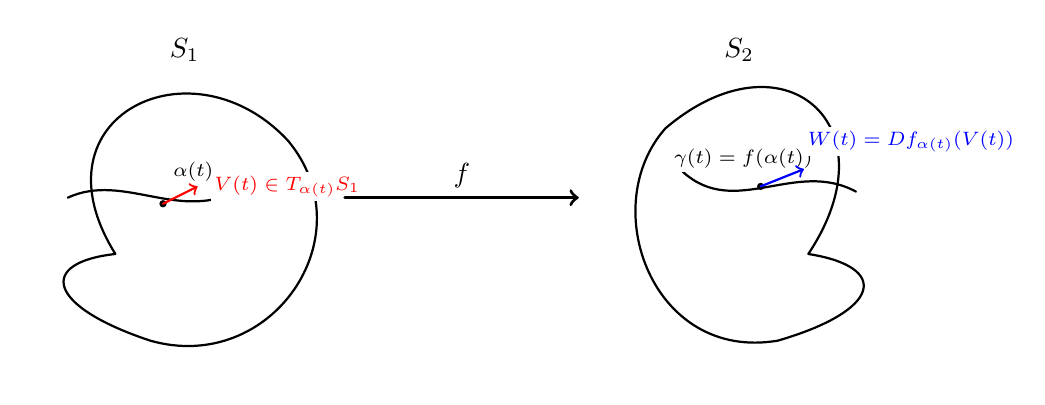
\begin{tikzpicture}[scale=1.1, line cap=round, line join=round]
		
		% ---------- Left surface S1 ----------
		\draw[thick]
		(-4,0) .. controls (-5,1.6) and (-3.1,2.5) .. (-2.0,1.3)
		.. controls (-1.1,0.2) and (-2.2,-1.4) .. (-3.6,-1.0)
		.. controls (-4.8,-0.6) and (-4.9,-0.1) .. (-4,0);
		\node at (-3.2,2.35) {$S_1$};
		
		% curve alpha on S1
		\draw[thick]
		(-4.55,0.65) .. controls (-3.9,0.95) and (-3.25,0.35) .. (-2.55,0.75);
		
		% label alpha
		\node[font=\scriptsize, fill=white, inner sep=1.2pt]
		at (-3.10,0.95) {$\alpha(t)$};
		
		% point and vector V on S1 (colored)
		\fill (-3.45,0.58) circle (1.2pt);
		\draw[->,thick,red] (-3.45,0.58) -- (-3.05,0.78);
		
		% label V (colored, off the curve)
		\node[font=\scriptsize, fill=white, inner sep=1.2pt, anchor=west, text=red]
		at (-2.90,0.78) {$V(t)\in T_{\alpha(t)}S_1$};
		
		% ---------- Map arrow f ----------
		\draw[->,very thick] (-1.35,0.65) -- (1.35,0.65);
		\node[above] at (0,0.65) {$f$};
		
		% ---------- Right surface S2 ----------
		\draw[thick]
		(4,0) .. controls (5,1.5) and (3.7,2.6) .. (2.35,1.45)
		.. controls (1.55,0.55) and (2.2,-1.25) .. (3.65,-1.0)
		.. controls (4.85,-0.65) and (4.95,-0.15) .. (4,0);
		\node at (3.2,2.35) {$S_2$};
		
		% curve gamma on S2
		\draw[thick]
		(2.55,0.95) .. controls (3.15,0.40) and (3.85,1.10) .. (4.55,0.72);
		
		% gamma label
		\node[font=\scriptsize, fill=white, inner sep=1.2pt]
		at (3.25,1.10) {$\gamma(t)=f(\alpha(t))$};
		
		% point and vector W on S2 (colored)
		\fill (3.45,0.78) circle (1.2pt);
		\draw[->,thick,blue] (3.45,0.78) -- (3.95,0.98);
		
		% W label moved up + colored (key change: yshift)
		\node[
		font=\scriptsize,
		fill=white,
		inner sep=1.2pt,
		anchor=west,
		text=blue,
		yshift=10pt
		] at (3.95,0.98) {$W(t)=Df_{\alpha(t)}(V(t))$};
		
	\end{tikzpicture}
	\caption{An isometry $f$ pushes forward a vector field $V$ along $\alpha$ to the vector field
		$W(t)=Df_{\alpha(t)}(V(t))$ along $\gamma=f\circ\alpha$.}
\end{figure}

	\par\medskip\noindent\textbf{Levi--Civita connection}\par\smallskip

	
	Let $(M,g)$ be a Riemannian manifold (in particular, a regular surface with the first fundamental form).
	A \emph{connection} on $TM$ is a map
	\[
	\nabla:\Gamma(TM)\times \Gamma(TM)\to \Gamma(TM),\qquad (X,Y)\mapsto \nabla_X Y,
	\]
	called the \emph{covariant derivative}, such that for all smooth functions $f$ and vector fields $X,Y,Z$:
	\begin{enumerate}
		\item $\nabla_{fX+Y}Z = f\nabla_X Z + \nabla_Y Z$,
		\item $\nabla_X(Y+Z)=\nabla_XY+\nabla_XZ$,
		\item $\nabla_X(fY)=X(f)\,Y + f\nabla_XY$.
	\end{enumerate}
	
	\medskip
	There exists a unique connection $\nabla$ satisfying:
	\begin{enumerate}
		\item \textbf{Metric compatibility} $(\nabla g=0)$:
		\[
		X\langle Y,Z\rangle = \langle \nabla_X Y, Z\rangle + \langle Y,\nabla_X Z\rangle,
		\]
		\item \textbf{Torsion-free}:
		\[
		\nabla_X Y - \nabla_Y X = [X,Y].
		\]
	\end{enumerate}
	This unique connection is the \emph{Levi--Civita connection} of $(M,g)$.
	
	\medskip
	If $S\subset\mathbb{R}^3$ is a surface with unit normal $n$ and $\bar\nabla$ denotes the usual derivative in
	$\mathbb{R}^3$, then for tangent vector fields $X,Y$ on $S$ one has the decomposition
	\[
	\bar\nabla_X Y = \nabla_X Y + \mathrm{II}(X,Y)\,n,
	\qquad
	\mathrm{II}(X,Y)=\langle \bar\nabla_X Y, n\rangle,
	\]
	so $\nabla_XY$ is the tangential part of the ambient derivative.
	
	\medskip
	For a curve $\alpha:I\to M$ and a vector field $V$ along $\alpha$, the covariant derivative along $\alpha$ is
	\[
	\frac{DV}{dt}:=\nabla_{\alpha'(t)}V.
	\]
	A field $V$ is \emph{parallel} along $\alpha$ if $\frac{DV}{dt}=0$, and $\alpha$ is a \emph{geodesic} if
	\[
	\frac{D\alpha'}{dt}=\nabla_{\alpha'}\alpha'=0.
	\]
	
	\medskip
	In local coordinates $(u^1,u^2)$ with $\partial_i=\frac{\partial}{\partial u^i}$ one writes
	\[
	\nabla_{\partial_i}\partial_j=\Gamma^{k}_{ij}\,\partial_k,
	\qquad
	\nabla_{\partial_i}(Y^j\partial_j)
	=
	\left(\frac{\partial Y^k}{\partial u^i}+\Gamma^{k}_{ij}Y^j\right)\partial_k.
	\]
	
	\par\medskip\noindent\textbf{Explanation of the notation}\par\smallskip

	
	\begin{itemize}
		\item \textbf{The tangent bundle and vector fields.}
		For a smooth manifold (or surface) $M$, the \emph{tangent bundle} $TM$ is the union of all tangent spaces
		$T_pM$ over $p\in M$.
		The notation $\Gamma(TM)$ denotes the set of smooth sections of $TM$, i.e.\ the set of smooth \emph{vector fields}
		on $M$:
		\[
		X\in\Gamma(TM)\quad\Longleftrightarrow\quad X(p)\in T_pM \text{ for all }p\in M,\ \text{smoothly in }p.
		\]
		
		\item \textbf{A connection (covariant derivative).}
		A (linear) connection on $TM$ is a map
		\[
		\nabla:\Gamma(TM)\times \Gamma(TM)\to \Gamma(TM),
		\qquad
		(X,Y)\mapsto \nabla_X Y,
		\]
		which should be thought of as ``differentiate the vector field $Y$ in the direction of the vector field $X$''.
		It satisfies the usual linearity and Leibniz rules:
		\[
		\nabla_{fX+gX'}Y=f\nabla_XY+g\nabla_{X'}Y,\qquad
		\nabla_X(Y+Y')=\nabla_XY+\nabla_XY',\qquad
		\nabla_X(fY)=X(f)\,Y+f\nabla_XY.
		\]
		
		\item \textbf{The curve $\gamma=f\circ\alpha$.}
		If $\alpha:I\to S_1$ is a curve and $f:S_1\to S_2$ is a smooth map, then the \emph{image curve}
		\[
		\gamma:=f\circ\alpha:I\to S_2,\qquad \gamma(t)=f(\alpha(t)).
		\]
		By the chain rule, the tangent vectors satisfy
		\[
		\gamma'(t)=Df_{\alpha(t)}\bigl(\alpha'(t)\bigr),
		\]
		where $Df_{\alpha(t)}:T_{\alpha(t)}S_1\to T_{\gamma(t)}S_2$ is the differential (pushforward) of $f$ at $\alpha(t)$.
	\end{itemize}
	
	A (smooth) vector field on $M$ means a smooth \emph{tangent} vector field, i.e.\ a section of the tangent bundle:
	\[
	X\in \Gamma(TM)\quad\Longleftrightarrow\quad X:M\to TM,\ \ X(p)\in T_pM\ \text{for all }p\in M.
	\]
	If $M\subset\mathbb{R}^3$ is embedded, an ambient vector field $Y:M\to\mathbb{R}^3$ need not be tangent; it splits as
	$Y=Y^\top+Y^\perp$ into tangent and normal components.
	
	\par\medskip\noindent\textbf{Example (sphere).}\par\smallskip

	Let $M=S^2\subset\mathbb{R}^3$ be the unit sphere. Its unit normal at $p\in S^2$ is $n(p)=p$.
	Consider the ambient vector field $Y(p)=e_3=(0,0,1)$.
	In general $Y$ is not tangent to $S^2$.
	The normal component is the projection onto $n(p)$:
	\[
	Y^\perp(p)=\langle Y(p),n(p)\rangle n(p)=\langle e_3,p\rangle\,p=p_3\,p,
	\]
	and therefore the tangential component is
	\[
	Y^\top(p)=Y(p)-Y^\perp(p)=e_3-p_3\,p.
	\]
	One checks tangency by $\langle Y^\top(p),p\rangle=0$, hence $Y^\top(p)\in T_pS^2$.
	
	\par\medskip\noindent\textbf{Example (plane).}\par\smallskip

	Let $M=\{(x,y,0)\}\subset\mathbb{R}^3$ with unit normal $n=e_3$.
	For the ambient field $Y\equiv e_3$ we get
	\[
	Y^\perp=\langle e_3,n\rangle n=e_3,\qquad Y^\top=Y-Y^\perp=0,
	\]
	so $Y$ is purely normal to the plane.
	
	\par\medskip\noindent\textbf{Example (graph surface).}\par\smallskip

	Let $M$ be the graph $X(x,y)=(x,y,f(x,y))$. Then $X_x=(1,0,f_x)$, $X_y=(0,1,f_y)$ and a normal is
	$N=X_x\times X_y=(-f_x,-f_y,1)$.
	For an ambient constant field $Y\equiv e_1=(1,0,0)$ one has the decomposition
	\[
	Y^\perp=\langle Y,n\rangle n,\qquad Y^\top=Y-\langle Y,n\rangle n,
	\quad\text{where } n=\frac{N}{\|N\|}.
	\]
	Unless $f_x\equiv 0$, the field $Y$ is not tangent to $M$.
	
	A (tangent) vector field on $M$ is a smooth section of the tangent bundle because it assigns to each point
	$p\in M$ a vector based at $p$ lying in the tangent space at $p$:
	\[
	X\in\Gamma(TM)\quad\Longleftrightarrow\quad X:M\to TM,\ \ X(p)\in T_pM\ \text{for all }p,
	\ \text{and } \pi\circ X=\mathrm{id}_M,
	\]
	where $\pi:TM\to M$ is the bundle projection.
	For a surface, $T_pM$ is the tangent plane at $p$.
	
	
	$\Gamma(TM)$ denotes the set of smooth tangent vector fields on $M$, i.e.\ maps $X:M\to TM$ with
	$X(p)\in T_pM$ for every $p\in M$.
	
	A connection is a map
	\[
	\nabla:\Gamma(TM)\times\Gamma(TM)\to\Gamma(TM),\qquad (X,Y)\mapsto \nabla_XY,
	\]
	so $\nabla_XY$ is again a tangent vector field. In particular, for each $p\in M$,
	\[
	(\nabla_XY)(p)\in T_pM.
	\]
	Heuristically, $(\nabla_XY_bt)(p)$ measures the variation of $Y$ at $p$ in the direction $X(p)$.
	Along a curve $\alpha(t)$ and a field $V(t)\in T_{\alpha(t)}M$, one writes
	\[
	\frac{DV}{dt}:=\nabla_{\alpha'(t)}V\in T_{\alpha(t)}M.
	\]
	
	The covariant derivative $\nabla_XY$ is the ``directional derivative'' of the vector field $Y$ in the direction $X$,
	defined intrinsically on $M$. It is a vector field, so for each $p\in M$ one has
	\[
	(\nabla_XY)(p)\in T_pM.
	\]
	Geometrically, $(\nabla_XY)(p)$ measures how $Y$ changes when one moves away from $p$ in the direction $X(p)$,
	using the connection to compare vectors in different tangent spaces.
	
	Equivalently, if $c(t)$ is any curve with $c(0)=p$ and $c'(0)=X(p)$ and $P_t:T_pM\to T_{c(t)}M$ denotes parallel
	transport along $c$, then
	\[
	(\nabla_XY)(p)
	=
	\left.\frac{d}{dt}\right|_{t=0}\Bigl(P_t^{-1}(Y(c(t)))\Bigr).
	\]
	Along a curve $\alpha(t)$ and a field $V(t)\in T_{\alpha(t)}M$, one writes
	\[
	\frac{DV}{dt}:=\nabla_{\alpha'(t)}V,
	\]
	so $DV/dt=0$ means that $V$ is parallel along $\alpha$, and $\nabla_{\alpha'}\alpha'=0$ means that $\alpha$ is a
	geodesic.
	
	\par\medskip\noindent\textbf{Example on $S^2$: computing $\nabla_{\alpha'}V$ by projection}\par\smallskip

	
	If $S\subset\mathbb{R}^3$ is a surface with unit normal $n$, then along a curve $\alpha(t)\subset S$ and a tangent
	field $V(t)\in T_{\alpha(t)}S$ one can compute the Levi--Civita covariant derivative by
	\[
	\frac{DV}{dt}=\left(\frac{dV}{dt}\right)^\top
	=
	\frac{dV}{dt}-\left\langle \frac{dV}{dt},\,n(\alpha(t))\right\rangle n(\alpha(t)).
	\]
	For the unit sphere $S^2$, one has $n(p)=p$.
	
	\par\medskip\noindent\textbf{(A) Great circle (equator) is a geodesic.}\par\smallskip

	Let $\alpha(s)=(\cos s,\sin s,0)$ (arc-length parametrization). Then
	\[
	T(s)=\alpha'(s)=(-\sin s,\cos s,0),\qquad \frac{dT}{ds}=(-\cos s,-\sin s,0).
	\]
	Since $n(\alpha(s))=\alpha(s)$,
	\[
	\left\langle \frac{dT}{ds},\,\alpha(s)\right\rangle
	= (-\cos s,-\sin s,0)\cdot(\cos s,\sin s,0)=-1.
	\]
	Hence
	\[
	\frac{DT}{ds}
	=
	\frac{dT}{ds}-\left\langle \frac{dT}{ds},\alpha\right\rangle\alpha
	=
	(-\cos s,-\sin s,0)-(-1)\,(\cos s,\sin s,0)=0,
	\]
	so $\nabla_TT=0$ and the equator is a geodesic.
	
	\par\medskip\noindent\textbf{(B) Latitude is not a geodesic (except the equator).}\par\smallskip

	Fix $\theta\in(0,\pi/2)$ and consider
	\[
	\alpha(\varphi)=\bigl(\cos\theta\cos\varphi,\ \cos\theta\sin\varphi,\ \sin\theta\bigr).
	\]
	Then $|\alpha'(\varphi)|=\cos\theta$, and the unit tangent is
	\[
	T(\varphi)=\frac{\alpha'(\varphi)}{|\alpha'(\varphi)|}=(-\sin\varphi,\cos\varphi,0).
	\]
	Differentiate:
	\[
	\frac{dT}{d\varphi}=(-\cos\varphi,-\sin\varphi,0),
	\qquad
	\left\langle \frac{dT}{d\varphi},\,\alpha(\varphi)\right\rangle=-\cos\theta.
	\]
	Therefore the tangential projection is
	\[
	\left(\frac{dT}{d\varphi}\right)^\top
	=
	\frac{dT}{d\varphi}-\left\langle \frac{dT}{d\varphi},\alpha\right\rangle\alpha
	=
	(-\cos\varphi,-\sin\varphi,0)+\cos\theta\,\alpha(\varphi)\neq 0
	\quad(\theta\neq 0).
	\]
	Since $ds=\cos\theta\,d\varphi$, we have
	\[
	\frac{DT}{ds}=\frac{1}{\cos\theta}\left(\frac{dT}{d\varphi}\right)^\top\neq 0\quad(\theta\neq 0),
	\]
	so a latitude circle is not a geodesic, except when $\theta=0$ (the equator).
	
	\par\medskip\noindent\textbf{How to understand a connection (Earth / sphere intuition)}\par\smallskip

	
	Think of $M=S^2$ (Earth idealized as a sphere). A wind (velocity) field is a \emph{tangent} vector field
	\[
	Y\in \Gamma(TM),\qquad Y(p)\in T_pS^2\ \text{for each }p\in S^2,
	\]
	so at every point you have an arrow lying in the local tangent plane.
	
	\medskip
	\noindent
	\textbf{Why we need a connection.}
	If $p$ and $q$ are two nearby points, then $T_pS^2$ and $T_qS^2$ are different tangent planes. Hence one cannot
	directly form $Y(q)-Y(p)$, because these vectors live in different vector spaces.
	
	\medskip
	\noindent
	\textbf{Role of the connection.}
	A connection $\nabla$ provides a rule to compare vectors in different tangent planes and therefore defines a
	directional derivative of vector fields. Given a tangent direction $X(p)\in T_pS^2$, the covariant derivative
	\[
	(\nabla_XY)(p)\in T_pS^2
	\]
	measures how $Y$ changes at $p$ when one moves in the direction $X(p)$, after correcting for the curvature of the
	surface.
	
	\medskip
	\noindent
	\textbf{Parallel transport interpretation.}
	Let $c(t)$ be a curve on $S^2$ with $c(0)=p$ and $c'(0)=X(p)$, and let
	$P_t:T_pS^2\to T_{c(t)}S^2$ denote parallel transport along $c$ (for the Levi--Civita connection).
	Then
	\[
	(\nabla_XY)(p)
	=
	\left.\frac{d}{dt}\right|_{t=0}\Bigl(P_t^{-1}(Y(c(t)))\Bigr).
	\]
	Here $P_t^{-1}(Y(c(t)))$ is the vector $Y(c(t))$ moved back to the original tangent space $T_pS^2$, so the usual
	difference quotient makes sense.
	
	\medskip
	\noindent
	\textbf{Geodesics.}
	For a curve $c(t)$, its velocity $T=c'(t)$ is tangent. The curve is a geodesic iff
	\[
	\nabla_TT=0,
	\]
	meaning its tangent vector is parallel along the curve (``straightest possible motion on the surface'').
	
	\par\medskip\noindent\textbf{How to understand a connection (Earth / sphere intuition)}\par\smallskip

	
	Think of $M=S^2$ (Earth idealized as a sphere). A wind (velocity) field is a \emph{tangent} vector field
	\[
	Y\in \Gamma(TM),\qquad Y(p)\in T_pS^2\ \text{for each }p\in S^2,
	\]
	so at every point you have an arrow lying in the local tangent plane.
	
	\medskip
	\noindent
	\textbf{Why we need a connection.}
	If $p$ and $q$ are two nearby points, then $T_pS^2$ and $T_qS^2$ are different tangent planes. Hence one cannot
	directly form $Y(q)-Y(p)$, because these vectors live in different vector spaces.
	
	\medskip
	\noindent
	\textbf{Role of the connection.}
	A connection $\nabla$ provides a rule to compare vectors in different tangent planes and therefore defines a
	directional derivative of vector fields. Given a tangent direction $X(p)\in T_pS^2$, the covariant derivative
	\[
	(\nabla_XY)(p)\in T_pS^2
	\]
	measures how $Y$ changes at $p$ when one moves in the direction $X(p)$, after correcting for the curvature of the
	surface.
	
	\medskip
	\noindent
	\textbf{Parallel transport interpretation.}
	Let $c(t)$ be a curve on $S^2$ with $c(0)=p$ and $c'(0)=X(p)$, and let
	$P_t:T_pS^2\to T_{c(t)}S^2$ denote parallel transport along $c$ (for the Levi--Civita connection).
	Then
	\[
	(\nabla_XY)(p)
	=
	\left.\frac{d}{dt}\right|_{t=0}\Bigl(P_t^{-1}(Y(c(t)))\Bigr).
	\]
	Here $P_t^{-1}(Y(c(t)))$ is the vector $Y(c(t))$ moved back to the original tangent space $T_pS^2$, so the usual
	difference quotient makes sense.
	
	\medskip
	\noindent
	\textbf{Geodesics.}
	For a curve $c(t)$, its velocity $T=c'(t)$ is tangent. The curve is a geodesic iff
	\[
	\nabla_TT=0,
	\]
	meaning its tangent vector is parallel along the curve (``straightest possible motion on the surface'').
	
	\par\medskip\noindent\textbf{What the connection gives you}\par\smallskip

	
	A connection $\nabla$ provides a consistent way to:
	\begin{enumerate}
		\item \textbf{compare vectors in different tangent planes}, and therefore
		\item \textbf{define a derivative} of a vector field.
	\end{enumerate}
	
	\par\medskip\noindent\textbf{``Derivative in a direction'' (the meaning of $\nabla_XY$)}\par\smallskip

	
	Pick:
	\begin{itemize}
		\item a direction of motion $X(p)\in T_pS^2$ (for example: your walking direction),
		\item and a tangent vector field $Y$ (for example: wind velocity).
	\end{itemize}
	Then $(\nabla_XY)(p)\in T_pS^2$ means:
	\begin{quote}
		Start at $p$, move a tiny bit in the direction $X(p)$.
		Bring the vector $Y$ at the new point back to the original tangent plane (using the connection's
		\emph{``keep direction as constant as possible''} rule).
		The rate of change of the difference is $(\nabla_XY)(p)$.
	\end{quote}
	
	\medskip
	\noindent
	\textbf{Parallel transport formula.}
	Let $c(t)$ be a curve with $c(0)=p$ and $c'(0)=X(p)$, and let
	$P_t:T_pS^2\to T_{c(t)}S^2$ denote parallel transport along $c$.
	Then
	\[
	(\nabla_XY)(p)
	=
	\left.\frac{d}{dt}\right|_{t=0}\Bigl(P_t^{-1}(Y(c(t)))\Bigr).
	\]
	
	% ------------------------------------------------------------
	\par\medskip\noindent\textbf{Chart 1: the spherical-triangle loop (holonomy picture)}\par\smallskip

	
	\begin{figure}[htbp]
		\centering
		\begin{tikzpicture}[scale=1.15, line cap=round, line join=round, >=Latex]
			
			% Sphere boundary (schematic 2D projection)
			\def\R{3.0}
			\draw[thick] (0,0) circle (\R);
			\node at (0,3.35) {$S^2$};
			
			% Key points: A, B on equator; N at "north pole"
			\coordinate (A) at (\R,0);
			\coordinate (B) at (-\R,0);
			\coordinate (N) at (0,\R);
			
			\fill (A) circle (1.2pt) node[below right] {$A$};
			\fill (B) circle (1.2pt) node[below left] {$B$};
			\fill (N) circle (1.2pt) node[above] {$N$};
			
			% Equator (AB)
			\draw[very thick] (B) -- (A);
			\node[below] at (0,-0.15) {\scriptsize equator};
			
			% Meridian-like arcs (schematic curves inside the disk)
			\draw[very thick]
			(A) .. controls (1.7,1.2) and (0.9,2.2) .. (N);
			\draw[very thick]
			(N) .. controls (-0.9,2.2) and (-1.7,1.2) .. (B);
			
			\node[font=\scriptsize, fill=white, inner sep=1.2pt] at (1.25,1.95) {meridian};
			\node[font=\scriptsize, fill=white, inner sep=1.2pt] at (-1.25,1.95) {meridian};
			
			% Direction of travel (arrows on edges)
			\draw[->] ($(A)!0.55!(N)$) -- ($(A)!0.62!(N)$);
			\draw[->] ($(N)!0.55!(B)$) -- ($(N)!0.62!(B)$);
			\draw[->] ($(B)!0.55!(A)$) -- ($(B)!0.62!(A)$);
			
			% Vectors being transported (schematic)
			% At A: point "north" (toward N)
			\draw[->,thick,blue] (A) -- ($(A)+( -0.55,0.75)$);
			\node[blue, font=\scriptsize, anchor=west] at ($(A)+(-0.55,0.75)$) {$V(A)$};
			
			% At B: show rotated vector (schematic)
			\draw[->,thick,blue] (B) -- ($(B)+(0.75,0.45)$);
			\node[blue, font=\scriptsize, anchor=east] at ($(B)+(0.75,0.45)$) {$V(B)$};
			
			% At A again: show "mismatch" after loop (schematic)
			\draw[->,thick,blue!60!black] ($(A)+(0.0,-0.05)$) -- ($(A)+(0.75,0.25)$);
			\node[blue!60!black, font=\scriptsize, anchor=west] at ($(A)+(0.75,0.25)$) {$V(A)$ after loop};
			
		\end{tikzpicture}
		\caption{Schematic spherical triangle loop $A\to N\to B\to A$.
			Parallel transport ($\nabla_{c'}V=0$ along each edge) can rotate the vector after returning to $A$
			(\emph{holonomy}), reflecting curvature.}
	\end{figure}
	
	% ------------------------------------------------------------
	\par\medskip\noindent\textbf{Chart 2: covariant derivative via parallel transport (diagram)}\par\smallskip

	
\[
\begin{tikzcd}[column sep=huge, row sep=large]
	T_pM \arrow[r,"P_t"] & T_{c(t)}M \\
	Y(p)\arrow[r,mapsto] \arrow[dr, phantom, "\text{compare in }T_pM" description] &
	Y(c(t)) \arrow[d,"P_t^{-1}"] \\
	& P_t^{-1}\!\bigl(Y(c(t))\bigr)\in T_pM
\end{tikzcd}
\]

	\[
	(\nabla_XY)(p)=\left.\frac{d}{dt}\right|_{t=0}\Bigl(P_t^{-1}(Y(c(t)))\Bigr),
	\qquad c(0)=p,\ c'(0)=X(p).
	\]
	
	
	% Preamble needs:
	% \usepackage{tikz}
	% \usepackage{tikz-3dplot}
	% \usetikzlibrary{calc}
	
	\begin{figure}[htbp]
		\centering
		
		% viewing angles: adjust if you want more/less "tilt"
		
		\begin{tikzpicture}[scale=1.15, line cap=round, line join=round, >=Latex]
			
			\def\R{2.8}
			
			% --- Sphere outline (schematic) ---
			\shade[ball color=gray!15, opacity=0.35] (0,0,0) circle (\R);
			\draw[thick] (0,0,0) circle (\R);
			\node at (0,0,\R+0.45) {$S^2$};
			
			% --- A,B on equator; N at north pole ---
			\coordinate (A) at (\R,0,0);      % lon 0 on equator
			\coordinate (B) at (0,\R,0);      % lon 90 on equator
			\coordinate (N) at (0,0,\R);      % north pole
			
			\fill (A) circle (1.2pt);
			\fill (B) circle (1.2pt);
			\fill (N) circle (1.2pt);
			
			\node[anchor=west] at ($(A)+(0.15,-0.10,0)$) {$A$};
			\node[anchor=south] at ($(B)+(0,0.10,0)$) {$B$};
			\node[anchor=south] at ($(N)+(0,0,0.12)$) {$N$};
			
			% --- Some faint meridians (optional, for 3D feel) ---
			% great circle in x-z plane (y=0)
			\draw[thin, gray!60] plot[domain=0:360, samples=120]
			({\R*cos(\x)},{0},{\R*sin(\x)});
			% great circle in y-z plane (x=0)
			\draw[thin, gray!60] plot[domain=0:360, samples=120]
			({0},{\R*cos(\x)},{\R*sin(\x)});
			
			% --- Spherical triangle edges ---
			% A -> N (meridian in x-z plane, y=0)
			\draw[very thick]
			plot[domain=0:90, samples=80]
			({\R*cos(\x)},{0},{\R*sin(\x)});
			
			% N -> B (meridian in y-z plane, x=0)
			\draw[very thick]
			plot[domain=90:0, samples=80]
			({0},{\R*cos(\x)},{\R*sin(\x)});
			
			% B -> A (equator arc in z=0 plane, from lon 90 to lon 0)
			\draw[very thick]
			plot[domain=90:0, samples=80]
			({\R*cos(\x)},{\R*sin(\x)},{0});
			
			% Direction arrows along edges
			\draw[->] plot[domain=35:42, samples=2]
			({\R*cos(\x)},{0},{\R*sin(\x)});
			\draw[->] plot[domain=55:48, samples=2]
			({0},{\R*cos(\x)},{\R*sin(\x)});
			\draw[->] plot[domain=55:48, samples=2]
			({\R*cos(\x)},{\R*sin(\x)},{0});
			
			% --- Vectors indicating parallel transport / holonomy (schematic) ---
			% At A: initial vector V(A) (blue) in tangent plane at A (e.g. "east" direction ~ +y)
			\draw[->, thick, blue] (A) -- ($(A)+(0,0.85,0)$);
			\node[blue, font=\scriptsize, fill=white, inner sep=1.2pt, anchor=west]
			at ($(A)+(0,0.85,0)$) {$V(A)$};
			
			% At B: transported vector (schematic)
			\draw[->, thick, blue] (B) -- ($(B)+(-0.70,0,0.35)$);
			\node[blue, font=\scriptsize, fill=white, inner sep=1.2pt, anchor=east]
			at ($(B)+(-0.70,0,0.35)$) {$V(B)$};
			
			% At N: transported vector (schematic; tangent plane at N is horizontal)
			\draw[->, thick, blue] (N) -- ($(N)+(0.75,-0.25,0)$);
			\node[blue, font=\scriptsize, fill=white, inner sep=1.2pt, anchor=west]
			at ($(N)+(0.75,-0.25,0)$) {$V(N)$};
			
			% Back at A: "after loop" vector (rotated) (blue!60!black) to show holonomy
			\draw[->, thick, blue!60!black] (A) -- ($(A)+(0,0,0.85)$);
			\node[blue!60!black, font=\scriptsize, fill=white, inner sep=1.2pt, anchor=west]
			at ($(A)+(0,0,0.85)$) {$V(A)\ \text{after loop}$};
			
			% Small label
			\node[font=\scriptsize, fill=white, inner sep=1.4pt]
			at (0.15,0.25,1.55) {parallel transport around $A\to N\to B\to A$};
			
		\end{tikzpicture}
		
		\caption{A 3D-looking schematic of a spherical triangle loop. A tangent vector field transported with
			$\nabla_{c'(t)}V=0$ along the loop can return rotated at $A$ (holonomy), reflecting curvature.}
	\end{figure}


\par\medskip\noindent\textbf{Parallel transport and directional derivative of a tangent field}\par\smallskip


On a manifold (in particular on a surface) tangent vectors at different points live in
different vector spaces. Thus, for a curve $c(t)$ with $c(0)=p$,
the expression $Y(c(t)) - Y(p)$ does not make sense intrinsically because
$Y(c(t))\in T_{c(t)}M$ while $Y(p)\in T_pM$.

\medskip
Let $P_t:T_pM\to T_{c(t)}M$ denote the (Levi--Civita) parallel transport along $c$
from $0$ to $t$. Then $P_t^{-1}:T_{c(t)}M\to T_pM$ brings vectors back to $T_pM$,
so that subtraction and differentiation become meaningful.

\medskip
\textbf{Definition (covariant derivative via parallel transport).}
Let $X(p)=c'(0)\in T_pM$ and let $Y$ be a tangent vector field along $c$.
The covariant derivative of $Y$ in the direction $X$ at $p$ is
\[
(\nabla_X Y)(p)
:=\left.\frac{d}{dt}\right|_{t=0}\Bigl(P_t^{-1}(Y(c(t)))\Bigr).
\]
Equivalently: transport $Y(c(t))$ back to $T_pM$ without twisting (parallel transport),
then differentiate in the fixed vector space $T_pM$.

\medskip
\textbf{Directional derivative: scalar vs.\ vector.}
For a scalar field $f:M\to\mathbb{R}$, the directional derivative is
\[
X(f)(p)=\left.\frac{d}{dt}\right|_{t=0} f(c(t)).
\]
For a tangent vector field $Y$, the intrinsic directional derivative is $\nabla_X Y$,
because one must compare vectors lying in different tangent planes.

\medskip
\textbf{Example (Earth as a sphere).}
Let $M=S^2$ model the Earth.
Let $X$ be a velocity field of motion on $S^2$ and let $Y$ be a wind field,
so $X(p),Y(p)\in T_pS^2$ for each $p\in S^2$.
Then $(\nabla_X Y)(p)$ measures the rate of change of the wind vector observed along the motion:
move from $p$ in the direction $X(p)$, parallel-transport the wind vector back to $T_pS^2$,
and differentiate.

In particular, if $Y=X$, then $\nabla_X X$ is the intrinsic acceleration of the motion.
A curve $c$ is a geodesic iff $\nabla_{c'}c'=0$, i.e.\ it has zero intrinsic acceleration.

\par\medskip\noindent\textbf{Example on the Earth sphere (equator): velocity field $X$ and wind field $Y$}\par\smallskip


Model the Earth as the unit sphere $S^2\subset\mathbb{R}^3$ with the induced (round) metric.
Fix a point on the equator, for instance
\[
p=(1,0,0)\in S^2.
\]
Then the tangent plane at $p$ is
\[
T_pS^2=\{v\in\mathbb{R}^3:\ v\cdot p=0\}=\{(0,a,b):a,b\in\mathbb{R}\}.
\]
A convenient orthonormal basis of $T_pS^2$ is given by
\[
E(p)=(0,1,0)\qquad\text{(east, along the equator)},\qquad
N(p)=(0,0,1)\qquad\text{(north, toward the north pole)}.
\]

\medskip
\textbf{Equator curve and ``right/left'' approach.}
Consider the equator (a great circle) through $p$:
\[
c(t)=(\cos t,\ \sin t,\ 0),\qquad c(0)=p,\qquad c'(0)=(0,1,0)=E(p).
\]
Approaching $p$ from $t>0$ versus $t<0$ corresponds to approaching from opposite sides along the
equator (east vs.\ west). If $Y$ is a tangent vector field, then reversing direction flips the sign:
\[
(\nabla_{-E}Y)(p)=-(\nabla_EY)(p).
\]

\medskip
\textbf{Why parallel transport is needed.}
For $t\neq 0$ one has $Y(c(t))\in T_{c(t)}S^2$, while $Y(p)\in T_pS^2$, so the difference
$Y(c(t))-Y(p)$ is not intrinsic. Let $P_t:T_pS^2\to T_{c(t)}S^2$ denote parallel transport along $c$.
Then the covariant derivative (directional derivative of a tangent field) is
\[
(\nabla_{E}Y)(p)
=\left.\frac{d}{dt}\right|_{t=0}\Bigl(P_t^{-1}\bigl(Y(c(t))\bigr)\Bigr)\in T_pS^2.
\]
Interpretation: bring the wind vector back to the fixed tangent plane $T_pS^2$ without twisting,
then differentiate there.

\medskip
\textbf{Ambient formula on the sphere (projection of the Euclidean derivative).}
Viewing $Y$ as a vector-valued function on $S^2$ with values in $\mathbb{R}^3$ and extending it
smoothly to a neighbourhood in $\mathbb{R}^3$, one has on $S^2$:
\[
\nabla_X Y=\Pi_{T_pS^2}\bigl(D_X Y\bigr),
\]
where $D_XY$ is the usual directional derivative in $\mathbb{R}^3$ and
\[
\Pi_{T_pS^2}(v)=v-(v\cdot p)\,p
\]
is the orthogonal projection onto $T_pS^2$.

\medskip
\textbf{Two guiding interpretations.}
\begin{itemize}
	\item If $Y=X$, then $\nabla_XX$ is the \emph{intrinsic acceleration}. A curve $c$ is a geodesic iff
	$\nabla_{c'}c'=0$. In particular, the equator is a great circle, hence a geodesic, so the velocity
	field along it satisfies $\nabla_EE=0$.
	\item If $Y$ represents a wind field (e.g.\ ``always pointing north'' along the equator), then
	$\nabla_EY$ measures how that wind vector changes as you move east, after correcting for the
	rotation of tangent planes by parallel transport.
\end{itemize}

\par\medskip\noindent\textbf{Parallel transport as a section of the restricted tangent bundle}\par\smallskip


Let $M$ be a surface (e.g.\ $S^2$) and let $c:[0,T]\to M$ be a smooth curve.
For each $t$ the tangent space $T_{c(t)}M$ is a different vector space. The collection of all
these tangent spaces along the curve is the restriction (pullback) of the tangent bundle to $c$:
\[
c^{*}(TM)
=\{(t,v): t\in[0,T],\ v\in T_{c(t)}M\}.
\]
One may think of $c^{*}(TM)$ as a ``slice'' of the tangent bundle $TM$ along the curve, i.e.\ the
family of tangent planes $\{T_{c(t)}M\}_{t\in[0,T]}$ stacked over the interval $[0,T]$.

\medskip
A \textbf{vector field along $c$} is precisely a \textbf{section} of this restricted bundle:
\[
V:[0,T]\to TM,\qquad V(t)\in T_{c(t)}M \ \ \text{for all }t.
\]

\medskip
Let $\nabla$ be the Levi--Civita connection on $M$.
Given an initial vector $v\in T_{c(0)}M$, there exists a unique vector field $V(t)$ along $c$
such that
\[
V(0)=v,\qquad \nabla_{c'(t)}V(t)=0\quad\text{for all }t,
\]
and this $V$ is called the \textbf{parallel vector field} along $c$ with initial value $v$.

\medskip
\textbf{Definition (parallel transport).}
The parallel transport along $c$ from $0$ to $t$ is the linear isomorphism
\[
P_{0\to t}:T_{c(0)}M\longrightarrow T_{c(t)}M,\qquad
P_{0\to t}(v):=V(t),
\]
where $V$ is the unique parallel vector field along $c$ satisfying $V(0)=v$.
More generally, for $s,t\in[0,T]$ one writes $P_{s\to t}:T_{c(s)}M\to T_{c(t)}M$, with
\[
P_{t\to t}=\mathrm{Id},\qquad P_{s\to u}=P_{t\to u}\circ P_{s\to t}.
\]

	
	
	% Problems 4--7 (Solutions)
\end{solution}

\begin{problem}[CP-VII-0072 --- Parallel transport on the sphere and holonomy of a latitude]
\label{prob:cp-vii-0072}
Let \(S^2\subset\mathbb{R}^3\) be the unit sphere with its standard metric.
Fix a latitude
\[
\gamma(\phi)=
(\sin\theta_0\cos\phi,\sin\theta_0\sin\phi,\cos\theta_0),
\qquad 0\le \phi\le 2\pi,
\]
where \(0<\theta_0<\pi\).

\begin{enumerate}
\item Compute the geodesic curvature \(k_g\) of the latitude.
\item Use Gauss--Bonnet on the spherical cap bounded by \(\gamma\) to determine
the net rotation angle of a tangent vector after parallel transport once
around \(\gamma\).
\item Check the result for the equator.
\end{enumerate}
\end{problem}

\begin{solution}
The latitude is a Euclidean circle of radius \(\sin\theta_0\).
With the orientation induced from the cap containing the north pole,
its geodesic curvature is constant:
\[
k_g=\cot\theta_0.
\]
Since
\[
ds=\sin\theta_0\,d\phi,
\]
we obtain
\[
\int_\gamma k_g\,ds
=
\int_0^{2\pi}
\cot\theta_0\,\sin\theta_0\,d\phi
=
2\pi\cos\theta_0.
\]

For the unit sphere, \(K\equiv1\). The area of the cap is
\[
A=2\pi(1-\cos\theta_0).
\]
Gauss--Bonnet gives
\[
\int_{\text{cap}}K\,dA+\int_\gamma k_g\,ds=2\pi,
\]
that is,
\[
2\pi(1-\cos\theta_0)+2\pi\cos\theta_0=2\pi.
\]

The holonomy angle around a positively oriented simple loop on a surface is,
modulo \(2\pi\), the curvature integral enclosed by the loop. Hence
\[
\boxed{\Delta\alpha
\equiv
2\pi(1-\cos\theta_0)\pmod{2\pi}}.
\]
For the equator, \(\theta_0=\pi/2\), so the enclosed area is \(2\pi\) and
\(\Delta\alpha\equiv0\pmod{2\pi}\), as expected.
\end{solution}

\subsection*{Main-text correspondence: VII/25}

\begin{problem}[CP-VII-0073 --- Problem 4 --- Curvature as vertical commutator and small-square holonomy]
\label{prob:cp-vii-0073}
Fix a $G$-bundle $\pi:P\to B$ with a connection $A$.
\begin{enumerate}[label=(\alph*)]
	\item Given vector fields $v,w$ on $B$, let $\hat v,\hat w$ denote their (unique) horizontal lifts to $P$.
	Show that the vertical component of $[\hat v,\hat w]$ at a point $p$ is
	\[
	p\cdot\bigl(-F(\hat v,\hat w)\bigr).
	\]
	\item Take local coordinates on $B$ around $\pi(p)$, and define $\gamma(t)$ to be the result of parallel transporting $p$
	for time $t$ in the $x^i$-direction, then time $t$ in the $x^j$-direction, then the other two sides of the square.
	Show that
	\[
	\dot\gamma(0)=0
	\qquad\text{and}\qquad
	\ddot\gamma(0)=p\cdot\bigl(-2F(u_i,u_j)\bigr),
	\]
	where $u_i$ and $u_j$ are any lifts of $\partial_{x^i}$ and $\partial_{x^j}$ to $p$.
\end{enumerate}
\end{problem}

\begin{solution}
Let $A\in\Omega^1(P,\mathfrak{g})$ be the connection form and let the curvature be
\[
F=dA+\tfrac12[A\wedge A].
\]

\textbf{(a)}
Since $\hat v$ and $\hat w$ are horizontal,
\[
A(\hat v)=0
\qquad\text{and}\qquad
A(\hat w)=0.
\]
Thus
\[
F(\hat v,\hat w)
=
dA(\hat v,\hat w)
=
\hat v\bigl(A(\hat w)\bigr)-\hat w\bigl(A(\hat v)\bigr)-A([\hat v,\hat w])
=
-A([\hat v,\hat w]).
\]
Hence
\[
A([\hat v,\hat w])=-F(\hat v,\hat w).
\]
The vertical component of a tangent vector $X\in T_pP$ is the fundamental vertical vector
\[
\bigl(A(X)\bigr)^\#_p,
\]
so
\[
\bigl([\hat v,\hat w]\bigr)^{\mathrm{vert}}_p
=
\bigl(A([\hat v,\hat w])\bigr)^\#_p
=
\bigl(-F(\hat v,\hat w)\bigr)^\#_p
=
p\cdot\bigl(-F(\hat v,\hat w)\bigr).
\]

\textbf{(b)}
Let $u_i,u_j$ be the horizontal lifts of $\partial_{x^i},\partial_{x^j}$ at $p$, and let $\Phi_i^t,\Phi_j^t$ be their flows.
The parallel-transport around the coordinate square can be written as the commutator of flows
\[
\gamma(t)
=
\Phi_j^{-t}\circ \Phi_i^{-t}\circ \Phi_j^{t}\circ \Phi_i^{t}(p).
\]
Standard flow-commutator calculus gives
\[
\dot\gamma(0)=0
\qquad\text{and}\qquad
\ddot\gamma(0)=2\,[u_i,u_j]_p.
\]
Moreover,
\[
\pi_*[u_i,u_j]=[\pi_*u_i,\pi_*u_j]=[\partial_{x^i},\partial_{x^j}]=0,
\]
so $[u_i,u_j]_p$ is vertical. By part (a),
\[
[u_i,u_j]_p
=
p\cdot\bigl(-F(u_i,u_j)\bigr).
\]
Therefore
\[
\ddot\gamma(0)
=
2[u_i,u_j]_p
=
p\cdot\bigl(-2F(u_i,u_j)\bigr).
\]

% -------------------------
% Problem 5
% -------------------------
\end{solution}

\subsection*{Main-text correspondence: VII/26}

\begin{problem}[CP-VII-0074 --- Problem 11. Curvature, geodesics, and local isometry]
\label{prob:cp-vii-0074}
Let $S_1$ and $S_2$ be surfaces with Gauss curvature $K_{S_1}, K_{S_2}$ respectively.
	\begin{enumerate}
		\item Suppose $f:S_1\to S_2$ is a diffeomorphism with $K_{S_2}(f(x))=K_{S_1}(x)$. Must $f$ be an isometry?
		\item Suppose that for any geodesic $\gamma:I\to S_1$ parametrised by arc-length, $f\circ\gamma:I\to S_2$ is also a geodesic
		parametrised by arc-length. Must $f$ be an isometry?
		\item Let $p_1\in S_1, p_2\in S_2$. Suppose $S_1$ and $S_2$ are locally isometric around $p_1$ and $p_2$.
		Show that there exists a geodesic $\gamma_1(t)$ emanating from $p_1$ and $\gamma_2(t)$ emanating from $p_2$ such that
		$K_{S_1}(\gamma_1(t))=K_{S_2}(\gamma_2(t))$, and such that if $\alpha_i(t)$ is a geodesic emanating from $p_i$ and making an
		angle $\theta$ from $\gamma_i$ (for fixed $\theta$), then $K_{S_1}(\alpha_1(t))=K_{S_2}(\alpha_2(t))$.
		Here all geodesics are parametrised by arc-length.
		\item Show conversely that if the above property is satisfied, then the $S_i$ are locally isometric near the $p_i$.
		Deduce that if $S_1$ and $S_2$ have constant curvature $K_{S_1}=K_{S_2}$, then $S_1$ and $S_2$ are locally isometric.
	\end{enumerate}
	\hfill\textit{Hint: Consider geodesic polar coordinates and solve an ODE for $G$.}
	
	\medskip
\end{problem}

\begin{solution}
\begin{enumerate}
		\item \textbf{Not necessarily.}
		Take $S_1=S_2=\mathbb{S}^2$ (unit sphere). Then $K\equiv 1$, so $K_{S_2}(f(x))=K_{S_1}(x)$ holds for every diffeomorphism
		$f:\mathbb{S}^2\to\mathbb{S}^2$. Most diffeomorphisms are not isometries (they distort lengths/areas), hence the condition on
		curvature alone does not force $f$ to be an isometry.
		
		\item \textbf{Yes.}
		Fix $p\in S_1$ and let $v\in T_pS_1$ be a unit tangent vector. Let $\gamma_v$ be the unit-speed geodesic with
		$\gamma_v(0)=p$ and $\gamma_v'(0)=v$. By hypothesis, $f\circ\gamma_v$ is also unit-speed, hence
		\[
		\|df_p(v)\|_{S_2}
		=
		\|(f\circ\gamma_v)'(0)\|_{S_2}
		=
		1.
		\]
		Thus $df_p$ maps the unit sphere in $T_pS_1$ into the unit sphere in $T_{f(p)}S_2$, so it preserves norms.
		By linearity and scaling, $\|df_p(w)\|_{S_2}=\|w\|_{S_1}$ for all $w\in T_pS_1$. Therefore for all $u,v\in T_pS_1$,
		polarization gives
		\[
		\langle df_p(u),df_p(v)\rangle_{S_2}
		=
		\frac{\|df_p(u+v)\|^2-\|df_p(u)\|^2-\|df_p(v)\|^2}{2}
		=
		\frac{\|u+v\|^2-\|u\|^2-\|v\|^2}{2}
		=
		\langle u,v\rangle_{S_1}.
		\]
		Hence $df_p$ is an isometry on tangent spaces for every $p$, so $f$ is a local isometry, and since it is a diffeomorphism,
		$f$ is an isometry.
		
		\item \textbf{Property (iii) from a local isometry.}
		Assume $S_1$ and $S_2$ are locally isometric near $p_1,p_2$.
		Let $F:U_1\to U_2$ be a local isometry with $F(p_1)=p_2$.
		Choose any unit-speed geodesic $\gamma_1$ emanating from $p_1$ and define $\gamma_2:=F\circ\gamma_1$.
		Local isometries preserve arc-length and send geodesics to geodesics, so $\gamma_2$ is a unit-speed geodesic from $p_2$.
		Moreover Gauss curvature is intrinsic, so $K_{S_2}(F(x))=K_{S_1}(x)$ on $U_1$, hence
		\[
		K_{S_2}(\gamma_2(t))=K_{S_1}(\gamma_1(t)).
		\]
		If $\alpha_1$ is any unit-speed geodesic from $p_1$ making angle $\theta$ with $\gamma_1$, define $\alpha_2:=F\circ\alpha_1$.
		Angles are preserved by a local isometry, so $\alpha_2$ makes the same angle $\theta$ with $\gamma_2$, and again
		\[
		K_{S_2}(\alpha_2(t))=K_{S_1}(\alpha_1(t)).
		\]
		
		\item \textbf{Conversely, curvature data in polar coordinates determines the metric.}
		Fix $p\in S$ and introduce geodesic polar coordinates $(r,\theta)$ around $p$ (for $r$ small).
		In these coordinates the metric takes the form
		\[
		ds^2 = dr^2 + G(r,\theta)^2\,d\theta^2,
		\qquad
		G(0,\theta)=0,\quad G_r(0,\theta)=1.
		\]
		A standard computation (using the Levi-Civita connection in these coordinates) yields the ODE
		\[
		G_{rr}(r,\theta)+K(r,\theta)\,G(r,\theta)=0,
		\]
		where $K(r,\theta)$ is the Gauss curvature in the same polar coordinates.
		
		Assume the property from (iii): for each fixed direction $\theta$, the curvature functions along the corresponding radial
		geodesics agree between $S_1$ and $S_2$. Then the functions $G_1(r,\theta)$ and $G_2(r,\theta)$ satisfy the same ODE in $r$
		with the same initial conditions, hence
		\[
		G_1(r,\theta)=G_2(r,\theta)
		\]
		for $r$ small. Therefore the metrics coincide in these polar coordinates, so identifying points with the same $(r,\theta)$
		defines a local isometry near $p_1$ and $p_2$.
		
		In particular, if $K_{S_1}=K_{S_2}$ is constant, then $G$ is determined (locally) solely by this constant, so any two
		surfaces of the same constant Gauss curvature are locally isometric.
	\end{enumerate}
	
	\medskip
	\textbf{Examples.}
	\begin{enumerate}
		\item \textbf{Flat case.} The plane and the cylinder both have $K\equiv 0$ and are locally isometric (unwrap the cylinder).
		\item \textbf{Positive curvature.} Any surface with $K\equiv K_0>0$ is locally isometric to the sphere of radius
		$1/\sqrt{K_0}$.
		\item \textbf{Negative curvature.} Any surface with constant $K_0<0$ is locally isometric to the hyperbolic plane of
		curvature $K_0$.
	\end{enumerate}
\end{solution}

\begin{problem}[CP-VII-0075 --- Problem 2 (Curvature from the length of small geodesic circles).]
\label{prob:cp-vii-0075}
Using geodesic polar coordinates, show that for a surface \(S\) and any point \(p\in S\), the Gaussian curvature can be expressed as
\[
K(p)=\lim_{r\to 0}\frac{3\bigl(2\pi r-L(r)\bigr)}{\pi r^{3}},
\]
where \(L(r)\) denotes the length of the geodesic circle of radius \(r\) centered at \(p\).
\emph{[Hint: Taylor expansion.]}
\end{problem}

\begin{solution}
Fix \(p\in S\). In \emph{geodesic polar coordinates} \((r,\theta)\) around \(p\), the metric has the form
\[
ds^{2}=dr^{2}+G(r,\theta)^{2}\,d\theta^{2},
\]
with \(G(0,\theta)=0\) and \(G_{r}(0,\theta)=1\). The geodesic circle of radius \(r\) is \(\{r=\text{const}\}\), and its length is
\[
L(r)=\int_{0}^{2\pi} \sqrt{g_{\theta\theta}}\,d\theta=\int_{0}^{2\pi} G(r,\theta)\,d\theta.
\]

A standard fact from Jacobi field theory is that \(G\) satisfies (along each fixed \(\theta\))
\[
G_{rr}(r,\theta)+K(r,\theta)\,G(r,\theta)=0,
\]
where \(K(r,\theta)\) is the Gaussian curvature at the point \(\exp_p(r\,e_\theta)\).
Since \(K(r,\theta)=K(p)+O(r)\) as \(r\to 0\), a Taylor expansion using
\[
G(0,\theta)=0,\quad G_r(0,\theta)=1,\quad G_{rr}(0,\theta)=0,\quad
G_{rrr}(0,\theta)=-K(p)
\]
gives
\[
G(r,\theta)=r-\frac{K(p)}{6}\,r^{3}+o(r^{3})\qquad (r\to 0),
\]
uniformly in \(\theta\). Integrating over \(\theta\),
\[
L(r)=\int_{0}^{2\pi}\left(r-\frac{K(p)}{6}r^{3}+o(r^{3})\right)d\theta
=2\pi r-\frac{K(p)}{6}\,2\pi r^{3}+o(r^{3}).
\]
Hence
\[
2\pi r-L(r)=\frac{K(p)}{6}\,2\pi r^{3}+o(r^{3})=\frac{K(p)\pi}{3}\,r^{3}+o(r^{3}),
\]
so
\[
\lim_{r\to 0}\frac{3(2\pi r-L(r))}{\pi r^{3}}
=\lim_{r\to 0}\frac{3\left(\frac{K(p)\pi}{3}r^{3}+o(r^{3})\right)}{\pi r^{3}}
=K(p),
\]
which is exactly the desired formula.


\par\medskip\noindent\textbf{Theory (for Problem 2: curvature from the length of small geodesic circles)}\par\smallskip


Let \(S\) be a smooth surface with Riemannian metric \(ds^{2}\), and fix a point \(p\in S\).
For sufficiently small \(r>0\), the exponential map \(\exp_{p}\) is a diffeomorphism from a
disk in \(T_{p}S\) onto a neighborhood of \(p\). Using \(\exp_{p}\), one introduces
\emph{geodesic polar coordinates} \((r,\theta)\) around \(p\), where \(r\) is the geodesic
distance from \(p\) and \(\theta\) is the direction in \(T_{p}S\).

\medskip
\noindent\textbf{(1) Polar form of the metric.}
In geodesic polar coordinates, the metric takes the form
\[
ds^{2}=dr^{2}+G(r,\theta)^{2}\,d\theta^{2},
\]
where \(G(r,\theta)>0\) for \(r>0\), and the initial conditions at \(r=0\) are
\[
G(0,\theta)=0,\qquad G_{r}(0,\theta)=1.
\]
Geometrically, \(G(r,\theta)\) is the length scale factor in the angular direction.

\medskip
\noindent\textbf{(2) Length of a geodesic circle.}
The geodesic circle of radius \(r\) centered at \(p\) is the curve \(\{r=\text{const}\}\).
Since \(g_{\theta\theta}=G(r,\theta)^{2}\), its length is
\[
L(r)=\int_{0}^{2\pi}\sqrt{g_{\theta\theta}}\,d\theta=\int_{0}^{2\pi}G(r,\theta)\,d\theta.
\]

\medskip
\noindent\textbf{(3) Jacobi equation for \(G\).}
For each fixed \(\theta\), the function \(r\mapsto G(r,\theta)\) satisfies the scalar
Jacobi equation
\[
G_{rr}(r,\theta)+K(r,\theta)\,G(r,\theta)=0,
\]
where \(K(r,\theta)\) is the Gaussian curvature at the point \(\exp_{p}(r\,e_{\theta})\).
This follows by considering the variation of radial geodesics with respect to \(\theta\)
and the associated Jacobi field.

\medskip
\noindent\textbf{(4) Small-\(r\) expansion and curvature.}
Since \(K(r,\theta)=K(p)+O(r)\) as \(r\to 0\), the Jacobi equation and the initial data imply
a Taylor expansion of the form
\[
G(r,\theta)=r-\frac{K(p)}{6}\,r^{3}+o(r^{3}) \qquad (r\to 0),
\]
uniformly in \(\theta\). Integrating this expansion over \(\theta\) yields the standard
asymptotic formula for the length of a small geodesic circle:
\[
L(r)=2\pi r-\frac{K(p)}{6}\,2\pi r^{3}+o(r^{3})
=2\pi r-\frac{K(p)\pi}{3}\,r^{3}+o(r^{3}).
\]
Rearranging gives the curvature-recovery limit used in Problem~2:
\[
K(p)=\lim_{r\to 0}\frac{3\bigl(2\pi r-L(r)\bigr)}{\pi r^{3}}.
\]


\bigskip
\end{solution}

\begin{problem}[CP-VII-0076 --- Problem 8(b) --- Vanishing curvature and Euclidean coordinates]
\label{prob:cp-vii-0076}
Show that the Riemann tensor of a Riemannian manifold $(X,g)$ vanishes iff $X$ can be covered by coordinate patches on which
\[
g=\sum_i (dx^i)^2.
\]
Such a metric is called \emph{flat}.
\textit{Hint:} Use the fact that if $\{v_i\}$ is a flat fibrewise basis of vector fields, then $v_i$ arises as coordinate vector fields $\partial_{x^i}$ iff $[v_i,v_j]=0$ for all $i,j$.
\end{problem}

\begin{solution}
$(\Rightarrow)$ Assume the Riemann curvature tensor $R$ of the Levi--Civita connection $\nabla$ is zero.
Let $U\subset X$ be a small contractible open set and choose $p\in U$.
Pick an orthonormal basis $\{e_1,\dots,e_n\}$ of $T_pX$.
Since $R=0$ and $U$ is contractible, parallel transport in $U$ is path-independent, hence defines smooth vector fields
$\{E_1,\dots,E_n\}$ on $U$ with
\[
\nabla E_i=0.
\]
Metric compatibility $\nabla g=0$ implies
\[
g(E_i,E_j)=\delta_{ij}
\]
on $U$.
Because $\nabla$ is torsion-free,
\[
0=T(E_i,E_j)=\nabla_{E_i}E_j-\nabla_{E_j}E_i-[E_i,E_j].
\]
Since $\nabla_{E_i}E_j=0$, we get
\[
[E_i,E_j]=0.
\]
By the stated fact, there exist local coordinates $(x^1,\dots,x^n)$ on $U$ such that
\[
E_i=\partial_{x^i}.
\]
Therefore
\[
g_{ij}=g(\partial_{x^i},\partial_{x^j})=g(E_i,E_j)=\delta_{ij},
\]
and hence
\[
g=\sum_i (dx^i)^2.
\]

$(\Leftarrow)$ Conversely, if on a coordinate patch we have
\[
g=\sum_i (dx^i)^2,
\]
then the metric components satisfy $g_{ij}=\delta_{ij}$, so all Christoffel symbols vanish,
\[
\Gamma^k_{ij}=0,
\]
and therefore the curvature tensor is zero,
\[
R=0.
\]

\par\medskip\noindent\textbf{Theory for Problem 8 --- Connections, torsion, curvature, and flatness}\par\smallskip


A (linear/affine) connection on $TX$ is an $\mathbb{R}$-bilinear map
\[
\nabla:\Gamma(TX)\times\Gamma(TX)\to\Gamma(TX),
\]
written $(v,w)\mapsto \nabla_v w$, such that
\[
\nabla_{fv}w=f\,\nabla_v w,
\]
\[
\nabla_v(fw)=v(f)\,w+f\,\nabla_v w.
\]

The torsion of $\nabla$ is the $(1,2)$-tensor
\[
T(v,w)=\nabla_v w-\nabla_w v-[v,w].
\]
In particular, the identity in Problem 8(a) is just a rearrangement of this definition.

The curvature of $\nabla$ is
\[
R(u,v)w=\nabla_u\nabla_v w-\nabla_v\nabla_u w-\nabla_{[u,v]}w.
\]
For the Levi--Civita connection (the unique connection with $\nabla g=0$ and $T=0$), this is the Riemann curvature tensor.

A Riemannian manifold is \emph{flat} if
\[
R=0.
\]
On a contractible open set, the condition $R=0$ implies parallel transport is path-independent, hence one can build a local frame $\{E_i\}$ such that
\[
\nabla E_i=0.
\]
Metric compatibility implies orthonormality is preserved, so
\[
g(E_i,E_j)=\delta_{ij}.
\]
If the connection is torsion-free, then
\[
0=T(E_i,E_j)=\nabla_{E_i}E_j-\nabla_{E_j}E_i-[E_i,E_j],
\]
and since $\nabla_{E_i}E_j=0$ this gives
\[
[E_i,E_j]=0.
\]
If a local frame satisfies $[E_i,E_j]=0$, then there exist local coordinates $(x^i)$ such that
\[
E_i=\partial_{x^i}.
\]
Hence
\[
g_{ij}=g(\partial_{x^i},\partial_{x^j})=\delta_{ij},
\]
so
\[
g=\sum_i (dx^i)^2.
\]
Conversely, if in coordinates $g_{ij}=\delta_{ij}$, then
\[
\Gamma^k_{ij}=0,
\]
so
\[
R=0.
\]

\par\medskip\noindent\textbf{Extended theory for Problem 8 --- Connections, torsion, curvature, and flatness}\par\smallskip


\textbf{Connections.}
A (linear/affine) connection on the tangent bundle $TX$ is an $\mathbb{R}$-bilinear map
\[
\nabla:\Gamma(TX)\times\Gamma(TX)\to\Gamma(TX),
\]
written $(v,w)\mapsto \nabla_v w$, such that for all $f\in C^\infty(X)$,
\[
\nabla_{fv}w=f\,\nabla_v w,
\]
\[
\nabla_v(fw)=v(f)\,w+f\,\nabla_v w.
\]

\textbf{Local expression.}
In local coordinates $(x^1,\dots,x^n)$, with $\partial_i=\partial_{x^i}$, define Christoffel symbols by
\[
\nabla_{\partial_i}\partial_j=\Gamma^k_{ij}\,\partial_k.
\]
For $v=v^i\partial_i$ and $w=w^j\partial_j$,
\[
\nabla_v w
=
\Bigl(v^i\partial_i w^k + v^i w^j \Gamma^k_{ij}\Bigr)\partial_k.
\]

\textbf{Lie bracket.}
The Lie bracket is determined by
\[
[v,w](f)=v(w(f))-w(v(f)).
\]
In coordinates,
\[
[v,w]
=
\Bigl(v^i\partial_i w^k-w^i\partial_i v^k\Bigr)\partial_k.
\]

\textbf{Torsion.}
The torsion tensor of $\nabla$ is
\[
T(v,w)=\nabla_v w-\nabla_w v-[v,w].
\]
In a coordinate basis,
\[
T(\partial_i,\partial_j)
=
\bigl(\Gamma^k_{ij}-\Gamma^k_{ji}\bigr)\partial_k.
\]

\textbf{Curvature.}
The curvature tensor is
\[
R(u,v)w=\nabla_u\nabla_v w-\nabla_v\nabla_u w-\nabla_{[u,v]}w.
\]
In coordinates,
\[
R(\partial_i,\partial_j)\partial_k
=
R^{\ell}{}_{kij}\,\partial_\ell,
\]
where
\[
R^{\ell}{}_{kij}
=
\partial_i\Gamma^\ell_{jk}
-
\partial_j\Gamma^\ell_{ik}
+
\Gamma^\ell_{im}\Gamma^m_{jk}
-
\Gamma^\ell_{jm}\Gamma^m_{ik}.
\]

\textbf{Levi--Civita connection.}
On a Riemannian manifold $(X,g)$ there is a unique connection satisfying
\[
\nabla g=0,
\]
\[
T=0.
\]
It is characterized by the Koszul formula
\[
2g(\nabla_u v,w)
=
u\,g(v,w)+v\,g(u,w)-w\,g(u,v)
+
g([u,v],w)-g([u,w],v)-g([v,w],u).
\]

\textbf{Flatness.}
A Riemannian manifold is \emph{flat} if
\[
R=0.
\]
On a contractible neighborhood, $R=0$ implies parallel transport is path-independent, hence there exist local fields $E_i$ such that
\[
\nabla E_i=0.
\]
Metric compatibility implies
\[
g(E_i,E_j)=\delta_{ij}.
\]
If $T=0$, then
\[
0=T(E_i,E_j)=\nabla_{E_i}E_j-\nabla_{E_j}E_i-[E_i,E_j],
\]
and therefore
\[
[E_i,E_j]=0.
\]
Commuting frames arise from coordinates, so there exist $(x^i)$ with
\[
E_i=\partial_{x^i}.
\]
Hence
\[
g_{ij}=g(\partial_{x^i},\partial_{x^j})=\delta_{ij},
\]
so
\[
g=\sum_i (dx^i)^2.
\]
Conversely, if $g_{ij}=\delta_{ij}$ in coordinates, then
\[
\Gamma^k_{ij}=0,
\]
and therefore
\[
R=0.
\]

% Problem 8 --- Chart 1
% ``Connection \\ensuremath{\\to} torsion & curvature'' dependency map
% Requires:
% \usepackage{tikz}
% \usetikzlibrary{arrows.meta,positioning}


\begin{figure}[h]
	\centering
	\begin{tikzpicture}[
		box/.style={draw, rounded corners, align=center, inner sep=6pt},
		arr/.style={-{Latex[length=2.5mm]}, thick},
		node distance=12mm
		]
		\node[box] (conn) {$\nabla$\\(connection)};
		\node[box, right=18mm of conn] (out) {$T$ and $R$\\(torsion, curvature)};
		\draw[arr] (conn) -- (out);
		
		\node[box, below=10mm of conn, text width=55mm] (lc) {Levi--Civita\\
			\[
			T=0
			\]
			\[
			\nabla g=0
			\]
		};
		
		\node[box, below=10mm of out, text width=55mm] (flat) {Flatness\\
			\[
			R=0
			\]
			\[
			\Longleftrightarrow
			\text{ locally } g=\sum_{i=1}^n (dx^i)^2
			\]
		};
		
		\draw[arr] (conn) -- (lc.north);
		\draw[arr] (out) -- (flat.north);
	\end{tikzpicture}
	
	\vspace{2mm}
	
	\[
	\begin{aligned}
		\nabla &\longmapsto (T,R),\\
		(T=0,\ \nabla g=0) &\Longleftrightarrow \text{Levi--Civita},\\
		R=0 &\Longleftrightarrow \text{locally } g=\sum_{i=1}^n (dx^i)^2.
	\end{aligned}
	\]
	\caption{Dependency map: a connection determines torsion and curvature; Levi--Civita and flatness are special conditions.}
\end{figure}



% Problem 8 --- Chart 2
% Parallelogram closure picture (torsion intuition)


\begin{figure}[h]
	\centering
	\begin{tikzpicture}[
		arr/.style={-{Latex[length=2.5mm]}, thick},
		dashedarr/.style={-{Latex[length=2.5mm]}, thick, dashed}
		]
		\coordinate (p) at (0,0);
		\coordinate (pv) at (3,0.3);
		\coordinate (pw) at (0.5,2.2);
		\coordinate (pvw) at ($(pv)+(0.5,2.2)$);
		\coordinate (pwv) at ($(pw)+(3,0.3)$);
		
		\fill (p) circle (1.5pt) node[below left] {$p$};
		
		\draw[arr] (p) -- (pv) node[midway, below] {$v$};
		\draw[arr] (p) -- (pw) node[midway, left] {$w$};
		
		\draw[arr] (pv) -- (pvw) node[midway, right] {$w$};
		\draw[arr] (pw) -- (pwv) node[midway, above] {$v$};
		
		% Endpoints (may differ if torsion/noncommutativity)
		\fill (pvw) circle (1.5pt) node[above right] {$p_{vw}$};
		\fill (pwv) circle (1.5pt) node[above left] {$p_{wv}$};
		
		% Gap vector
		\draw[dashedarr] (pwv) -- (pvw) node[midway, above] {gap};
		
		% [OK] FIX: no \[...\] inside node
		\node[align=left] at (1.7,-1.2) {$\displaystyle
			T(v,w)=\nabla_v w-\nabla_w v-[v,w]
			$};
	\end{tikzpicture}
	\caption{Torsion intuition: the failure of the ``parallelogram'' to close is captured by torsion (together with bracket effects).}
\end{figure}




% Problem 8 --- Chart 3
% Curvature as holonomy around a loop


\begin{figure}[h]
	\centering
	\begin{tikzpicture}[
		arr/.style={-{Latex[length=2.5mm]}, thick},
		loop/.style={thick}
		]
		\coordinate (p) at (0,0);
		
		% loop
		\draw[loop] (p) .. controls (1.8,1.2) and (2.0,-1.2) .. (p);
		\draw[arr] (1.2,0.75) -- (1.35,0.62); % direction marker
		
		\fill (p) circle (1.5pt) node[below left] {$p$};
		
		% initial vector u at p
		\draw[arr] (p) -- (0.9,0.9) node[midway, above left] {$u$};
		
		% returned vector u' at p (slightly rotated)
		\draw[arr] (p) -- (1.1,0.6) node[midway, below right] {$u'$};
		
		% [OK] FIX: do NOT use \[ ... \] inside a node
		\node[align=left] at (0,-2.0) {$\displaystyle u' - u \approx R(v,w)\,u$};
		
	\end{tikzpicture}
	\caption{Curvature intuition: parallel transport around a small loop changes a
		vector; the infinitesimal change is governed by curvature.}
\end{figure}




% Problem 8 --- Chart 4
% Flatness pipeline diagram (implication chain)


\begin{figure}[h]
	\centering
	\begin{tikzpicture}[
        scale=0.66,
        transform shape,
		box/.style={draw, rounded corners, align=center, inner sep=6pt, text width=37mm},
		arr/.style={-{Latex[length=2.5mm]}, thick},
		node distance=12mm
		]
		\node[box] (r0) {
			\[
			R=0
			\]
		};
		
		\node[box, right=5mm of r0] (pt) {
			path-independent\\parallel transport
		};
		
		\node[box, right=5mm of pt] (par) {
			exist local frame $\{E_i\}$
			\[
			\nabla E_i=0
			\]
		};
		
		\node[box, right=5mm of par] (comm) {
			torsion-free $\Rightarrow$
			\[
			[E_i,E_j]=0
			\]
		};
		
		\node[box, right=5mm of comm] (coords) {
			exist coordinates $(x^i)$
			\[
			E_i=\partial_{x^i}
			\]
		};
		
		\node[box, right=5mm of coords] (eucl) {
			\[
			g=\sum_{i=1}^n (dx^i)^2
			\]
		};
		
		\draw[arr] (r0) -- (pt);
		\draw[arr] (pt) -- (par);
		\draw[arr] (par) -- (comm);
		\draw[arr] (comm) -- (coords);
		\draw[arr] (coords) -- (eucl);
	\end{tikzpicture}
	
	\vspace{2mm}
	
	\[
	\begin{aligned}
		R=0
		&\Longrightarrow
		\text{path-independent parallel transport}
		\\
		&\Longrightarrow
		\exists\,\{E_i\}:\ \nabla E_i=0
		\\
		&\Longrightarrow
		[E_i,E_j]=0
		\\
		&\Longrightarrow
		E_i=\partial_{x^i}
		\\
		&\Longrightarrow
		g=\sum_{i=1}^n (dx^i)^2.
	\end{aligned}
	\]
	\caption{Flatness pipeline: vanishing curvature implies local Euclidean coordinates (and conversely).}
\end{figure}

\clearpage
\end{solution}

\subsection*{Main-text correspondence: VII/27}

\begin{problem}[CP-VII-0077 --- Ricci and scalar curvature of \(S^2(r)\times\mathbb{R}\)]
\label{prob:cp-vii-0077}
Let
\[
M=S^2(r)\times\mathbb{R}
\]
carry the product metric.  At a point choose an orthonormal frame
\(e_1,e_2,e_3\), where \(e_1,e_2\) are tangent to \(S^2(r)\) and
\(e_3\) is tangent to the \(\mathbb{R}\)-factor.

Using the sectional curvatures of a Riemannian product:

\begin{enumerate}
\item determine \(K(e_1,e_2)\), \(K(e_1,e_3)\), and \(K(e_2,e_3)\);
\item compute \(\operatorname{Ric}(e_i,e_i)\) for \(i=1,2,3\);
\item compute the scalar curvature \(S\);
\item decide whether the product metric is Einstein.
\end{enumerate}
\end{problem}

\begin{solution}
The round sphere of radius \(r\) has constant sectional curvature
\(1/r^2\).  A two-plane containing one direction from each factor of a
Riemannian product has sectional curvature zero.  Hence
\[
K(e_1,e_2)=\frac1{r^2},
\qquad
K(e_1,e_3)=K(e_2,e_3)=0.
\]

For an orthonormal frame,
\[
\operatorname{Ric}(e_i,e_i)
 =\sum_{j\ne i}K(e_i,e_j).
\]
Therefore
\[
\operatorname{Ric}(e_1,e_1)=\frac1{r^2},
\qquad
\operatorname{Ric}(e_2,e_2)=\frac1{r^2},
\qquad
\operatorname{Ric}(e_3,e_3)=0.
\]
All mixed components vanish in this product frame, so
\[
\operatorname{Ric}
=
\operatorname{diag}\!\left(\frac1{r^2},\frac1{r^2},0\right).
\]

Taking the trace gives
\[
S=\frac2{r^2}.
\]

An Einstein metric must satisfy \(\operatorname{Ric}=\lambda g\) for a
single scalar \(\lambda\).  Here the Ricci eigenvalues are
\(1/r^2,1/r^2,0\), so no such \(\lambda\) exists.  Thus
\(S^2(r)\times\mathbb{R}\) with the product metric is not Einstein.
\end{solution}

\subsection*{Main-text correspondence: VII/28}

\begin{problem}[CP-VII-0078 --- Constant sectional curvature has zero Weyl tensor]
\label{prob:cp-vii-0078}
Let \((M^n,g)\), \(n\ge4\), have constant sectional curvature \(K\), so
\[
R_{ijkl}
=
K\bigl(g_{ik}g_{jl}-g_{il}g_{jk}\bigr).
\]
Use
\[
W_{ijkl}
=
R_{ijkl}
-\frac1{n-2}
\left(
g_{ik}R_{jl}-g_{il}R_{jk}
-g_{jk}R_{il}+g_{jl}R_{ik}
\right)
+\frac{S}{(n-1)(n-2)}
\left(
g_{ik}g_{jl}-g_{il}g_{jk}
\right)
\]
to prove that \(W=0\).
\end{problem}

\begin{solution}
For constant sectional curvature,
\[
R_{ij}=(n-1)K\,g_{ij},
\qquad
S=n(n-1)K.
\]
Substitution into the middle term gives
\[
-\frac{2(n-1)K}{n-2}
\bigl(g_{ik}g_{jl}-g_{il}g_{jk}\bigr),
\]
while the scalar-curvature term becomes
\[
\frac{nK}{n-2}
\bigl(g_{ik}g_{jl}-g_{il}g_{jk}\bigr).
\]
Consequently the coefficient of
\(g_{ik}g_{jl}-g_{il}g_{jk}\) in \(W\) is
\[
K-\frac{2(n-1)K}{n-2}+\frac{nK}{n-2}=0.
\]
Hence
\[
\boxed{W=0}.
\]
Thus every constant-sectional-curvature metric is conformally flat in
dimension \(n\ge4\).
\end{solution}

\subsection*{Main-text correspondence: VII/34}

\begin{problem}[CP-VII-0079 --- Problem 7: Isometries and M\\"{o}bius maps on the 2--sphere]
\label{prob:cp-vii-0079}
Let $S^{2}\subset\mathbb{R}^{3}$ be the unit sphere with the standard round metric.
	
	\begin{enumerate}
		\item Let $f:S^{2}\to S^{2}$ be a diffeomorphism which is also a global isometry.
		Using that $f$ sends geodesics to geodesics (or otherwise), show that
		$f$ is the restriction to $S^{2}$ of an element of the orthogonal group $O(3)$.
		\item Identifying $\mathbb{C}\cup\{\infty\}$ with $S^{2}\subset\mathbb{R}^{3}$ via stereographic projection,
		prove that the M\"obius group $\operatorname{PSL}(2,\mathbb{C})$ acts on the abstract smooth surface $S^{2}$ by diffeomorphisms.
		
		\emph{Hint:} Check that the generators $z\mapsto az+b$ and $z\mapsto 1/z$ of the M\"obius group
		act smoothly from the original definition of smooth maps in terms of a smooth atlas.
		\item If a M\"obius map $A$ defines an isometry of $S^{2}$, show that it commutes with the antipodal map
		$a:S^{2}\to S^{2}$ given by $a(x,y,z)=(-x,-y,-z)$.
	\end{enumerate}
	
	\par\medskip\noindent\textbf{Theory / Background.}\par\smallskip

	
	\begin{itemize}
		\item The isometry group of the round sphere $(S^{2},g_{\mathrm{round}})$ is the group of restrictions of
		orthogonal transformations $A\in O(3)$.
		Great circles (intersections of $S^{2}$ with $2$--planes through the origin) are exactly the geodesics.
		\item For $p\in S^{2}$ the exponential map
		\[
		\exp_p:T_pS^{2}\to S^{2},\qquad
		\exp_p(v)=\cos |v|\;p+\sin |v|\;\frac{v}{|v|},
		\]
		is a diffeomorphism from $\{v\in T_pS^{2}:|v|<\pi\}$ onto $S^{2}\setminus\{-p\}$.
		\item Stereographic projection $\sigma:S^{2}\setminus\{N\}\to\mathbb{C}$ from the north pole $N$ is a smooth diffeomorphism
		and extends to a homeomorphism $\sigma:S^{2}\to\hat{\mathbb{C}}:=\mathbb{C}\cup\{\infty\}$, $\sigma(N)=\infty$.
		\item M\"obius transformations are maps
		\[
		z\longmapsto \frac{az+b}{cz+d},\qquad
		\begin{pmatrix}a&b\\c&d\end{pmatrix}\in\operatorname{SL}(2,\mathbb{C}),
		\]
		considered up to nonzero scalar multiples; they form the group $\operatorname{PSL}(2,\mathbb{C})$.
		The group is generated by translations $z\mapsto z+b$, dilations/rotations $z\mapsto az$, and inversion $z\mapsto 1/z$.
		\item Any linear map $B:\mathbb{R}^{3}\to\mathbb{R}^{3}$ commutes with the antipodal map $-\mathrm{id}$:
		$B(-x)=-B(x)$.
	\end{itemize}
\end{problem}

\begin{solution}
\par\medskip\noindent\textbf{(a) Isometries of $S^{2}$ come from $O(3)$.}\par\smallskip

	
	Let $f:S^{2}\to S^{2}$ be an isometry.
	
	\emph{Step 1: Extend the derivative.}
	Choose $p\in S^{2}$ and set $q=f(p)$.  
	Because $f$ is an isometry, its differential
	\[
	df_p:T_pS^{2}\to T_qS^{2}
	\]
	is an isometry of inner--product spaces.
	
	Choose orthonormal bases $\{e_1,e_2\}$ of $T_pS^{2}$ and $\{e'_1,e'_2\}$ of $T_qS^{2}$ such that
	$e'_i=df_p(e_i)$. Then $\{e_1,e_2,p\}$ and $\{e'_1,e'_2,q\}$ are orthonormal bases of $\mathbb{R}^{3}$.
	Define $A:\mathbb{R}^{3}\to\mathbb{R}^{3}$ by
	\[
	A(e_i)=e'_i,\qquad A(p)=q.
	\]
	In these bases the matrix of $A$ is orthogonal, so $A\in O(3)$.
	In particular $A(S^{2})=S^{2}$ and $A$ restricts to an isometry of $S^{2}$.
	
	\emph{Step 2: Reduce to an isometry fixing a point with identity derivative.}
	Define
	\[
	g := A^{-1}\circ f:S^{2}\to S^{2}.
	\]
	Then $g$ is an isometry, $g(p)=p$, and
	\[
	dg_p=(A^{-1})_{*}\circ df_p=\mathrm{id}_{T_pS^{2}}.
	\]
	
	\emph{Step 3: Show that $g=\mathrm{id}_{S^{2}}$.}
	Let $v\in T_pS^{2}$ with $|v|<\pi$. Let
	\[
	\gamma_v(t):=\exp_p(tv)
	\]
	be the unique geodesic with $\gamma_v(0)=p$, $\gamma'_v(0)=v$.
	Since $g$ is an isometry and $g(p)=p$, the curve $g\circ\gamma_v$ is a geodesic starting at $p$.
	Its initial velocity is
	\[
	(g\circ\gamma_v)'(0)=dg_p(\gamma_v'(0))=dg_p(v)=v,
	\]
	so $g\circ\gamma_v$ and $\gamma_v$ are geodesics with the same initial data.
	By uniqueness of geodesics, $g(\gamma_v(t))=\gamma_v(t)$ for all $t$ with $|t|<\pi$.
	
	The exponential map $\exp_p$ is a diffeomorphism from
	$\{v\in T_pS^{2}:|v|<\pi\}$ onto $S^{2}\setminus\{-p\}$, so
	\[
	g(x)=x\qquad\text{for all }x\in S^{2}\setminus\{-p\}.
	\]
	By continuity, $g(-p)=\lim_{t\to\pi^-}g(\gamma_v(t))
	=\lim_{t\to\pi^-}\gamma_v(t)=-p$, hence $g$ is the identity on all of $S^{2}$.
	
	\emph{Step 4: Conclusion.}
	We have $f=A\circ g=A|_{S^{2}}$, so $f$ is the restriction to $S^{2}$ of some $A\in O(3)$.
	
	\par\medskip\noindent\textbf{(b) The M\"obius group acts smoothly on $S^{2}$.}\par\smallskip

	
	Let $\sigma:S^{2}\to\hat{\mathbb{C}}$ be stereographic projection (extended by $\sigma(N)=\infty$).
	For $M\in\operatorname{PSL}(2,\mathbb{C})$ define
	\[
	\Phi_M := \sigma^{-1}\circ M\circ\sigma:S^{2}\to S^{2}.
	\]
	
	\emph{Group action.}
	Since $\sigma$ and $M$ are bijections, so is $\Phi_M$. For $M_1,M_2\in\operatorname{PSL}(2,\mathbb{C})$ we have
	\[
	\Phi_{M_1M_2}
	=\sigma^{-1}\circ M_1M_2\circ\sigma
	=(\sigma^{-1}\circ M_1\circ\sigma)\circ(\sigma^{-1}\circ M_2\circ\sigma)
	=\Phi_{M_1}\circ\Phi_{M_2},
	\]
	and clearly $\Phi_{\mathrm{id}}=\mathrm{id}_{S^{2}}$. Thus $\operatorname{PSL}(2,\mathbb{C})$ acts on $S^{2}$.
	
	\emph{Smoothness.}
	Consider the atlas $\{(U_0,\varphi_0),(U_1,\varphi_1)\}$ on $S^{2}$, where
	\[
	U_0=S^{2}\setminus\{N\},\quad \varphi_0=\sigma,\qquad
	U_1=S^{2}\setminus\{S\},\quad \varphi_1= z\mapsto \frac{1}{\sigma(z)}.
	\]
	A map $\Psi:S^{2}\to S^{2}$ is smooth iff each coordinate representation
	$\varphi_i\circ\Psi\circ\varphi_j^{-1}$ is smooth between open subsets of $\mathbb{C}$.
	
	The group $\operatorname{PSL}(2,\mathbb{C})$ is generated by
	\[
	T_{a,b}:z\mapsto az+b,\qquad I:z\mapsto 1/z.
	\]
	These maps are rational functions of $z$, hence smooth on the chart $U_0$.
	On the chart near $\infty$ (where we use coordinates $w=1/z$) their coordinate expressions
	remain rational (e.g.\ $w\mapsto w/(a+bw)$ for $z\mapsto az+b$), hence smooth.
	Therefore each generator induces a smooth diffeomorphism of $S^{2}$.
	
	Compositions and inverses of smooth diffeomorphisms are smooth diffeomorphisms.
	Hence for every $M\in\operatorname{PSL}(2,\mathbb{C})$ the map $\Phi_M$ is a diffeomorphism.
	Thus $\operatorname{PSL}(2,\mathbb{C})$ acts on $S^{2}$ by diffeomorphisms.
	
	\par\medskip\noindent\textbf{(c) Isometric M\"obius maps commute with the antipodal map.}\par\smallskip

	
	Suppose a M\"obius map $A$ induces an isometry of $(S^{2},g_{\mathrm{round}})$.
	By part~(b) this gives a diffeomorphism $f_A:S^{2}\to S^{2}$.
	Since $f_A$ is an isometry, part~(a) implies that there exists $B\in O(3)$ with
	\[
	f_A = B|_{S^{2}}.
	\]
	
	Let $a:S^{2}\to S^{2}$ be the antipodal map $a(x)=-x$.
	Because $B$ is linear, $B(-x)=-B(x)$ for all $x\in\mathbb{R}^{3}$.
	Hence, for every $x\in S^{2}$,
	\[
	f_A(a(x)) = B(-x) = -B(x) = a(B(x)) = a(f_A(x)).
	\]
	Thus $f_A\circ a = a\circ f_A$, i.e.\ the isometric M\"obius map commutes with the antipodal map.
	
	\par\medskip\noindent\textbf{Examples.}\par\smallskip

	
	\begin{enumerate}
		\item For $\theta\in\mathbb{R}$, the rotation
		\[
		R_\theta = \begin{pmatrix}
			\cos\theta & -\sin\theta & 0\\
			\sin\theta & \cos\theta & 0\\
			0          & 0          & 1
		\end{pmatrix}\in SO(3)
		\]
		restricts to an isometry of $S^{2}$. In stereographic coordinates $z=x+iy$ this corresponds
		to the M\"obius map $z\mapsto e^{i\theta}z$.
		\item The dilation $z\mapsto 2z$ is a M\"obius transformation but does not come from any
		$B\in O(3)$, hence its induced map on $S^{2}$ is not an isometry of the round metric.
		\item Every element of $SO(3)$ corresponds, via stereographic projection, to a M\"obius map of the form
		\[
		z\longmapsto \frac{\alpha z+\beta}{-\overline{\beta}\,z+\overline{\alpha}},\qquad
		|\alpha|^{2}+|\beta|^{2}=1,
		\]
		and these are precisely the orientation--preserving isometries of $S^{2}$.
	\end{enumerate}
	
	\par\medskip\noindent\textbf{M\\"{o}bius transformations, \texorpdfstring{$\mathrm{PSL}(2,\mathbb{C})$}{PSL(2,C)}, and the action on $S^{2}$}\par\smallskip

	
	In this subsection we explain in detail why the M\\"{o}bius group can be identified
	with $\mathrm{PSL}(2,\mathbb{C})$ and why, after identifying
	$\widehat{\mathbb{C}} = \mathbb{C}\cup\{\infty\}$ with $S^{2}\subset\mathbb{R}^3$
	via stereographic projection, this group acts on the abstract smooth surface
	$S^2$ by diffeomorphisms.
	
	\par\medskip\noindent\textbf{1. The Riemann sphere and stereographic projection}\par\smallskip

	
	We consider the unit sphere
	\[
	S^{2} = \{(x,y,t)\in\mathbb{R}^{3} : x^{2}+y^{2}+t^{2}=1\}.
	\]
	Let $N=(0,0,1)$ be the north pole, and let
	\[
	\Pi : S^{2}\setminus\{N\} \longrightarrow \mathbb{R}^{2}\cong\mathbb{C}
	\]
	be the stereographic projection from $N$ onto the plane $\{t=0\}$.  In
	coordinates one checks that
	\[
	\Pi(x,y,t) = \left( \frac{x}{1-t},\,\frac{y}{1-t} \right),
	\]
	so if we identify $\mathbb{R}^{2}$ with $\mathbb{C}$ via
	$(X,Y)\mapsto X+iY$, then
	\[
	\Pi(x,y,t) = z = \frac{x}{1-t} + i\,\frac{y}{1-t}.
	\]
	
	We extend $\Pi$ to a bijection
	\[
	\Phi : S^{2} \longrightarrow \widehat{\mathbb{C}} := \mathbb{C}\cup\{\infty\}
	\]
	by setting $\Phi(N) = \infty$ and $\Phi|_{S^{2}\setminus\{N\}} = \Pi$.
	This is a homeomorphism, and in fact a smooth diffeomorphism in the sense
	of smooth manifolds if we equip $\widehat{\mathbb{C}}$ with the standard
	structure of a 1--dimensional complex manifold (the Riemann sphere).  Its
	inverse $\Phi^{-1}:\widehat{\mathbb{C}}\to S^{2}$ is given by the classical
	formulas (for $z=x+iy\in\mathbb{C}$)
	\[
	\Phi^{-1}(z) =
	\left(
	\frac{2x}{|z|^{2}+1},\,
	\frac{2y}{|z|^{2}+1},\,
	\frac{|z|^{2}-1}{|z|^{2}+1}
	\right),
	\qquad
	\Phi^{-1}(\infty) = N.
	\]
	
	Thus $S^{2}$ and $\widehat{\mathbb{C}}$ are the same smooth surface, viewed
	in two different ways; we will freely pass between them via $\Phi$.
	
	\par\medskip\noindent\textbf{2. M\\"{o}bius transformations on the extended complex plane}\par\smallskip

	
	A \emph{M\\"{o}bius transformation} (or linear fractional transformation) is a
	map $f:\widehat{\mathbb{C}}\to\widehat{\mathbb{C}}$ of the form
	\[
	f(z) = \frac{az+b}{cz+d},
	\qquad a,b,c,d\in\mathbb{C},\quad ad-bc\neq 0,
	\]
	with the usual conventions
	\[
	f\!\left(-\frac{d}{c}\right) = \infty\quad (c\neq 0),\qquad
	f(\infty) =
	\begin{cases}
		\dfrac{a}{c}, & c\neq 0,\\[0.4em]
		\infty, & c=0.
	\end{cases}
	\]
	
	It is well known (and easy to check) that:
	
	\begin{itemize}
		\item M\\"{o}bius transformations form a group under composition;
		\item the map $z\mapsto z$ is the identity element;
		\item every M\\"{o}bius transformation is a homeomorphism of
		$\widehat{\mathbb{C}}$ with continuous inverse of the same form.
	\end{itemize}
	
	\par\medskip\noindent\textbf{3. M\\"{o}bius transformations and $2\times 2$ matrices}\par\smallskip

	
	To each M\\"{o}bius transformation $f(z)=\dfrac{az+b}{cz+d}$ we associate the
	matrix
	\[
	A =
	\begin{pmatrix}
		a & b\\
		c & d
	\end{pmatrix}
	\in \mathrm{GL}(2,\mathbb{C}).
	\]
	Composition of M\\"{o}bius transformations corresponds to matrix multiplication:
	if
	\[
	f_A(z) = \frac{az+b}{cz+d},\qquad
	f_B(z) = \frac{\alpha z+\beta}{\gamma z+\delta},
	\]
	then for all $z\in\widehat{\mathbb{C}}$ for which both sides are defined we
	have
	\[
	(f_B\circ f_A)(z) = f_{BA}(z),
	\]
	where $BA$ is the ordinary product of matrices.
	
	However, the matrix representation is not unique: multiplying the matrix by
	a nonzero scalar does not change the M\\"{o}bius transformation.  Indeed, if
	$\lambda\in\mathbb{C}^{\times}$, then
	\[
	f_{\lambda A}(z)
	= \frac{(\lambda a)z + \lambda b}{(\lambda c)z + \lambda d}
	= \frac{az+b}{cz+d}
	= f_{A}(z).
	\]
	Thus the same M\\"{o}bius map corresponds to the whole 1--dimensional family of
	matrices $\lambda A$, $\lambda\neq 0$.
	
	We remove this redundancy by working projectively.  First, note that we may
	restrict attention to matrices with determinant $1$:
	if $A\in\mathrm{GL}(2,\mathbb{C})$ has $\det A\neq 0$, then we may rescale
	$A$ to $\lambda A$ with $\lambda^2\det A = 1$, so that $\lambda A\in
	\mathrm{SL}(2,\mathbb{C})$.  This rescaling does not change $f_A$, so every
	M\\"{o}bius transformation is represented by \emph{some} matrix in
	$\mathrm{SL}(2,\mathbb{C})$.
	
	Moreover, within $\mathrm{SL}(2,\mathbb{C})$ the only nontrivial scalar
	multiple that preserves determinant $1$ is $-I$, since if
	$\lambda A\in\mathrm{SL}(2,\mathbb{C})$ with $A\in\mathrm{SL}(2,\mathbb{C})$,
	then
	\[
	1 = \det(\lambda A) = \lambda^{2}\det A = \lambda^2,
	\]
	so $\lambda = \pm 1$.  Thus the scalar redundancy inside
	$\mathrm{SL}(2,\mathbb{C})$ is precisely the central subgroup
	$\{\pm I\}$.
	
	We therefore define the \emph{projective special linear group}
	\[
	\mathrm{PSL}(2,\mathbb{C})
	:= \mathrm{SL}(2,\mathbb{C}) / \{\pm I\}.
	\]
	An element of $\mathrm{PSL}(2,\mathbb{C})$ is an equivalence class $[A]$ of
	matrices $A\in\mathrm{SL}(2,\mathbb{C})$, where $A\sim -A$.
	
	The assignment
	\[
	[A] \longmapsto f_A
	\]
	is a well-defined group homomorphism
	\[
	\mathrm{PSL}(2,\mathbb{C})
	\longrightarrow
	\{\text{M\\"{o}bius transformations on }\widehat{\mathbb{C}}\},
	\]
	which is bijective.  Hence we have a natural group isomorphism
	\[
	\mathrm{PSL}(2,\mathbb{C})
	\;\cong\;
	\{\text{all M\\"{o}bius transformations on }\widehat{\mathbb{C}}\}.
	\]
	This is the precise sense in which ``the M\\"{o}bius group is
	$\mathrm{PSL}(2,\mathbb{C})$''.
	
	From the complex--geometric viewpoint, $\widehat{\mathbb{C}}$ is the complex
	projective line $\mathbb{CP}^{1}$ and $\mathrm{PSL}(2,\mathbb{C})$ is the
	group of holomorphic automorphisms of $\mathbb{CP}^{1}$.
	
	\par\medskip\noindent\textbf{4. Generators of the M\\"{o}bius group}\par\smallskip

	
	It is a standard fact that the M\\"{o}bius group is generated by the following
	simple maps:
	\begin{align*}
		T_b(z) &= z + b, && b\in\mathbb{C} \quad\text{(translations)},\\
		D_a(z) &= a z,   && a\in\mathbb{C}^{\times}\quad\text{(dilations/rotations)},\\
		I(z)   &= \frac{1}{z}                     &&\text{(inversion)}.
	\end{align*}
	More precisely, any M\\"{o}bius transformation $f(z)=\dfrac{az+b}{cz+d}$ with
	$ad-bc\neq 0$ can be written as a finite composition of maps of the form
	$T_b$, $D_a$, and $I$.  For example, when $c\neq 0$ one checks that
	\[
	\frac{az+b}{cz+d} =
	D_{a/c}\circ T_{d/c}\circ I\circ T_{b/a}(z),
	\]
	and similar decompositions hold in all cases.  Thus, to understand the
	smoothness properties of general M\\"{o}bius maps, it suffices to understand
	these generators.
	
	\par\medskip\noindent\textbf{5. Induced maps on the sphere via stereographic projection}\par\smallskip

	
	Given any M\\"{o}bius transformation
	$f:\widehat{\mathbb{C}}\to\widehat{\mathbb{C}}$, we obtain a map
	\[
	F := \Phi^{-1}\circ f\circ\Phi : S^{2} \longrightarrow S^{2}.
	\]
	The exercise asks us to show that $F$ is a \emph{diffeomorphism} of the
	smooth surface $S^{2}$.  Since $\Phi$ and $\Phi^{-1}$ are already smooth
	diffeomorphisms, it is enough to check that $f$ is smooth with smooth
	inverse in the atlas on $\widehat{\mathbb{C}}$ coming from stereographic
	coordinates.
	
	The important observation is that smoothness of $F$ can be verified in
	local coordinates.  On the chart
	\[
	U = S^{2}\setminus\{N\},\qquad \Phi:U\to\mathbb{C},
	\]
	the coordinate expression of $F$ is
	\[
	\Phi\circ F\circ\Phi^{-1} = f:\mathbb{C}\to\mathbb{C},
	\]
	which is clearly smooth wherever it is defined (it is a rational function
	with denominator nonzero).  Near the point corresponding to $\infty$ we
	switch to another stereographic chart; in those coordinates the expression
	for $f$ is again rational, hence smooth, and the chart transition maps
	between the two stereographic charts are themselves M\\"{o}bius transformations
	(and therefore smooth).  This shows that $F$ is smooth in the sense of
	smooth manifolds.
	
	Because M\\"{o}bius transformations form a group under composition and inversion,
	$f$ has a M\\"{o}bius inverse $f^{-1}$, and therefore
	\[
	F^{-1} = \Phi^{-1}\circ f^{-1}\circ \Phi : S^{2}\to S^{2}
	\]
	is also smooth.  Consequently $F$ is a diffeomorphism.
	
	To make this completely concrete it is often convenient to verify the claim
	first for the generators $T_b$, $D_a$ and $I$, and then conclude for all
	M\\"{o}bius maps by composition.  We briefly spell this out.
	
	\par\medskip\noindent\textbf{Translations and dilations/rotations.}\par\smallskip

	Let $f(z)=az+b$ with $a\neq 0$.  Then on the chart $U$,
	\[
	\Phi\circ F\circ\Phi^{-1}(z) = f(z) = az+b,
	\]
	which is entire and hence smooth.  On the overlap with the second
	stereographic chart (from the south pole) the coordinate expression of $F$
	is the composition of $f$ with the smooth chart transition maps; it is
	therefore smooth as well.  The inverse map is represented by the affine map
	$f^{-1}(z) = a^{-1}(z-b)$, so $F$ is a diffeomorphism.
	
	\par\medskip\noindent\textbf{Inversion.}\par\smallskip

	Let $f(z) = 1/z$, extended by $f(0)=\infty$, $f(\infty)=0$.  On
	$\mathbb{C}^{\times}$ this is smooth.  In the stereographic chart $U$ away
	from the point $\Phi^{-1}(0)$ (the point corresponding to $z=0$) the map
	\[
	\Phi\circ F\circ\Phi^{-1}(z)=\frac{1}{z}
	\]
	is smooth.  Near $z=\infty$ we switch to the other stereographic chart,
	where the coordinate $w=1/z$ is finite; in that chart $f$ is simply
	$w\mapsto w$, so again we have a smooth expression.  The inverse of $f$ is
	itself ($f^{-1}=f$), so $F$ is a diffeomorphism of $S^{2}$.
	
	\medskip
	
	Since translation, dilation/rotation, and inversion each induce smooth
	diffeomorphisms of $S^{2}$ via
	\[
	F = \Phi^{-1}\circ f\circ\Phi,
	\]
	and every M\\"{o}bius transformation is a finite composition of these generators,
	we conclude:
	
	\begin{quote}
		For every $[A]\in\mathrm{PSL}(2,\mathbb{C})$ the corresponding M\\"{o}bius
		transformation $f_A$ determines a diffeomorphism
		\[
		F_A = \Phi^{-1}\circ f_A\circ\Phi : S^{2}\to S^{2}.
		\]
		The assignment $[A]\mapsto F_A$ defines a smooth action of
		$\mathrm{PSL}(2,\mathbb{C})$ on the abstract smooth surface $S^{2}$ by
		diffeomorphisms.
	\end{quote}
	
	Thus, identifying $\widehat{\mathbb{C}}$ with $S^{2}$ via stereographic
	projection, the M\\"{o}bius group $\mathrm{PSL}(2,\mathbb{C})$ acts on $S^{2}$
	smoothly and by diffeomorphisms, as required in part (b) of the problem.
\end{solution}

\begin{problem}[CP-VII-0080 --- Problem 4 (Isometries are determined by a point and differential)]
\label{prob:cp-vii-0080}
Let $S$ be a connected surface and $f,g:S\to S$ two isometries.
Assume that there exists $p\in S$ such that $f(p)=g(p)$ and $Df_p=Dg_p$.
Show that $f(q)=g(q)$ for all $q\in S$.

\medskip
\textbf{Theory.}
\begin{itemize}
	\item An isometry sends geodesics to geodesics.
	\item A geodesic is uniquely determined by initial data $(\gamma(0),\gamma'(0))$ (ODE uniqueness).
	\item In a normal neighbourhood of $p$, points are of the form $\exp_p(v)$ and radial geodesics are unique.
\end{itemize}

\medskip
\end{problem}

\begin{solution}
Define $h:=g^{-1}\circ f$. Then $h$ is an isometry and
\[
h(p)=g^{-1}(f(p))=g^{-1}(g(p))=p,
\qquad
Dh_p=D(g^{-1})_{g(p)}\circ Df_p=(Dg_p)^{-1}\circ Df_p=\mathrm{Id}.
\]
Let $v\in T_pS$ and let $\gamma_v$ be the geodesic with $\gamma_v(0)=p$ and $\gamma_v'(0)=v$.
Since $h$ is an isometry, $h\circ\gamma_v$ is a geodesic, and
\[
(h\circ\gamma_v)(0)=h(p)=p,\qquad (h\circ\gamma_v)'(0)=Dh_p(v)=v.
\]
Thus $h\circ\gamma_v$ and $\gamma_v$ satisfy the same geodesic equation with the same initial data,
so by uniqueness
\[
h(\gamma_v(t))=\gamma_v(t)
\]
for all $t$ for which $\gamma_v(t)$ stays in a normal neighbourhood of $p$.
Hence $h=\mathrm{Id}$ on some open neighbourhood $U$ of $p$.

Now let $F:=\{x\in S:\ h(x)=x\}$. The set $F$ is closed by continuity. It is open because if $x\in F$,
then the above geodesic argument applied at $x$ shows $h=\mathrm{Id}$ on a neighbourhood of $x$.
Since $F$ is nonempty (it contains $p$), open and closed, and $S$ is connected, we conclude $F=S$.
Therefore $h=\mathrm{Id}$ on $S$, i.e.\ $g^{-1}\circ f=\mathrm{Id}$, and so $f=g$ everywhere.

\medskip
\textbf{Example.}
On $\mathbb{R}^2$, any isometry is $x\mapsto Ax+b$ with $A\in O(2)$.
If $f(p)=g(p)$ and $Df_p=Dg_p$, then $A$ and $b$ coincide, hence $f=g$ globally.


\par\medskip\noindent\textbf{Theory for Problem 4 (Rigidity of isometries from 1-jet data)}\par\smallskip


Let $(S,\langle\cdot,\cdot\rangle)$ be a connected Riemannian surface and let $f:S\to S$ be an isometry.

\medskip
\textbf{(1) Metric preservation and orthogonality of the differential.}
By definition of isometry,
\[
\langle Df_p(X),Df_p(Y)\rangle_{f(p)}=\langle X,Y\rangle_p
\qquad\text{for all }p\in S,\;X,Y\in T_pS.
\]
Hence $Df_p:T_pS\to T_{f(p)}S$ is an orthogonal linear map (it preserves lengths and angles).

\medskip
\textbf{(2) Isometries preserve the Levi--Civita connection.}
If $\nabla$ denotes the Levi--Civita connection on $S$, then for all vector fields $X,Y$,
\[
Df(\nabla_X Y)=\nabla_{Df(X)}\,Df(Y).
\]
(Equivalently, $f$ is an affine map for $\nabla$.) This follows from the uniqueness of the Levi--Civita
connection as the unique torsion-free, metric-compatible connection.

\medskip
\textbf{(3) Isometries send geodesics to geodesics and preserve speed.}
A curve $\gamma$ is a geodesic iff $\nabla_{\dot\gamma}\dot\gamma=0$.
Using (2),
\[
\nabla_{\dot{(f\circ\gamma)}}\dot{(f\circ\gamma)}
= Df(\nabla_{\dot\gamma}\dot\gamma)=0,
\]
so $f\circ\gamma$ is geodesic whenever $\gamma$ is. Moreover, since $Df$ preserves norms,
\[
\|(f\circ\gamma)'(t)\|=\|Df_{\gamma(t)}(\gamma'(t))\|=\|\gamma'(t)\|,
\]
so in particular unit-speed geodesics are mapped to unit-speed geodesics.

\medskip
\textbf{(4) Uniqueness of geodesics from initial conditions.}
In local coordinates, geodesics satisfy the second-order ODE
\[
x^{k}{}'' + \Gamma^k_{ij}(x)\,x^i{}'x^j{}' = 0.
\]
Therefore, by standard ODE uniqueness, if two geodesics $\gamma,\eta$ satisfy
$\gamma(0)=\eta(0)$ and $\gamma'(0)=\eta'(0)$, then $\gamma=\eta$ on their common interval of existence.

\medskip
\textbf{(5) Exponential map and normal neighbourhoods (optional viewpoint).}
For $p\in S$ define $\exp_p(v)=\gamma_v(1)$, where $\gamma_v$ is the geodesic with
$\gamma_v(0)=p$ and $\gamma_v'(0)=v$.
For $\|v\|$ small, $\exp_p$ is a diffeomorphism onto a normal neighbourhood $U$ of $p$,
and each $q\in U$ lies on a unique geodesic segment issuing from $p$.

\medskip
\textbf{(6) Consequence (idea used in the proof of Problem 4).}
If two isometries agree at $p$ and have the same differential at $p$, then they send every geodesic
starting at $p$ with initial velocity $v$ to geodesics with the same initial data.
By (4) they coincide along these geodesics, hence they coincide on a neighbourhood of $p$,
and then (by connectedness) everywhere on $S$.

\par\medskip\noindent\textbf{Remark (``Rigidity'' and ``1-jet data'' in Problem 4)}\par\smallskip


\textbf{Rigidity (in this context).}
By \emph{rigidity} we mean that an isometry has no freedom once enough local data are fixed:
if two isometries $f,g:S\to S$ agree at one point $p$ and have the same differential at $p$,
then they must coincide everywhere on the connected surface $S$.
Equivalently, an isometry is completely determined by its first-order behaviour at a single point.

\medskip
\textbf{1-jet data.}
For a smooth map $f:S\to S$, the \emph{1-jet of $f$ at $p$} is the pair
\[
j_p^1 f \;:=\; \bigl(f(p),\, Df_p\bigr),
\]
consisting of the \emph{value} of $f$ at $p$ (zeroth-order data) and the \emph{differential}
of $f$ at $p$ (first-order data). Thus
\[
j_p^1 f = j_p^1 g
\quad\Longleftrightarrow\quad
f(p)=g(p)\ \text{ and }\ Df_p=Dg_p.
\]
Problem~4 states precisely that \emph{isometries are $1$-jet determined}:
on a connected surface, equality of $1$-jet data at one point forces $f=g$ on all of $S$.
\end{solution}

\section{Lorentzian Geometry}

\subsection*{Main-text correspondence: VII/29}

\begin{problem}[CP-VII-0081 --- Timelike, spacelike, and null vectors in Minkowski space]
\label{prob:cp-vii-0081}
On \(\mathbb{R}^{1,3}\) use the Lorentzian metric
\[
g=-dt^2+dx^2+dy^2+dz^2.
\]
Classify each vector as timelike, spacelike, or null:
\[
u=(2,1,1,0),\qquad
v=(1,2,0,0),\qquad
w=(\sqrt2,1,1,0).
\]
Then determine the equation of the null cone through the origin.
\end{problem}

\begin{solution}
For \(X=(X^0,X^1,X^2,X^3)\),
\[
g(X,X)=-(X^0)^2+(X^1)^2+(X^2)^2+(X^3)^2.
\]
Hence
\[
g(u,u)=-4+1+1=-2<0,
\]
so \(u\) is timelike;
\[
g(v,v)=-1+4=3>0,
\]
so \(v\) is spacelike; and
\[
g(w,w)=-2+1+1=0,
\]
so \(w\) is null.

A vector \((t,x,y,z)\) is null exactly when
\[
-t^2+x^2+y^2+z^2=0.
\]
Therefore the null cone is
\[
\boxed{t^2=x^2+y^2+z^2}.
\]
Unlike a positive-definite Riemannian metric, a Lorentzian metric thus
has nonzero vectors of zero squared length.
\end{solution}

\subsection*{Main-text correspondence: VII/30}

\begin{problem}[CP-VII-0082 --- Riemannian slices and null curves in a flat FLRW metric]
\label{prob:cp-vii-0082}
Consider the spatially flat FLRW metric
\[
ds^2=-dt^2+a(t)^2\bigl(dx^2+dy^2+dz^2\bigr),
\qquad a(t)>0.
\]

\begin{enumerate}
\item Find the metric induced on the hypersurface \(t=t_0\).
\item Show that for a comoving worldline \(x,y,z=\mathrm{const}\), proper
      time equals the coordinate time \(t\).
\item For a radial null curve, with
      \(dr^2=dx^2+dy^2+dz^2\), derive \(dr/dt\).
\item Explain one structural difference between the Lorentzian metric
      above and its induced Riemannian spatial metric.
\end{enumerate}
\end{problem}

\begin{solution}
On the slice \(t=t_0\) we have \(dt=0\), so
\[
ds_{\mathrm{slice}}^2
=
a(t_0)^2\bigl(dx^2+dy^2+dz^2\bigr).
\]
This is positive definite.

For a comoving worldline \(dx=dy=dz=0\), hence
\[
ds^2=-dt^2.
\]
With the convention \(ds^2=-d\tau^2\) on timelike worldlines,
\[
d\tau=dt
\]
for increasing \(t\).

For a radial null curve,
\[
0=-dt^2+a(t)^2dr^2,
\]
so
\[
\boxed{\frac{dr}{dt}=\pm\frac1{a(t)}}.
\]

The spacetime metric is indefinite and admits timelike and null
directions.  The induced metric on a constant-\(t\) spatial slice is
positive definite, so every nonzero tangent vector to the slice has
positive squared length.
\end{solution}

\section{Hyperbolic Geometry}

\subsection*{Main-text correspondence: VII/31}

\begin{problem}[CP-VII-0083 --- Problem 4 (Hyperbolic distance as a cross--ratio)]
\label{prob:cp-vii-0083}
Let $z_1,z_2$ be distinct points in the upper half plane $\mathbb{H}$.
	Suppose that the hyperbolic line through $z_1$ and $z_2$ meets the real axis
	at points $w_1$ and $w_2$, where $z_1$ lies on the hyperbolic line segment
	$w_1 z_2$ (and where one $w_i$ may be $\infty$).
	Show that the hyperbolic distance
	\[
	d_{\mathrm{hyp}}(z_1,z_2)=\log r,
	\]
	where $r$ is the cross-ratio of the four points $z_1,z_2,w_1,w_2$ taken in an
	appropriate order.
	
	\par\medskip\noindent\textbf{Theory (what we use).}\par\smallskip

	\begin{enumerate}
		\item In the upper half-plane model, the hyperbolic metric is
		\[
		ds=\frac{|dz|}{\Im z},
		\qquad
		dA=\frac{dx\,dy}{y^2}\quad (z=x+iy).
		\]
		\item The orientation-preserving isometries of $(\mathbb{H},ds)$ are exactly the M\\"{o}bius
		transformations with real coefficients:
		\[
		T(z)=\frac{az+b}{cz+d},\qquad a,b,c,d\in\R,\ ad-bc=1,
		\]
		i.e.\ $T\in \operatorname{PSL}(2,\R)$.
		\item The cross-ratio of four (possibly extended) complex numbers is
		\[
		[a,b,c,d]=\frac{(a-c)(b-d)}{(a-d)(b-c)},
		\]
		and it is invariant under M\\"{o}bius transformations:
		\[
		[T(a),T(b),T(c),T(d)]=[a,b,c,d].
		\]
	\end{enumerate}
\end{problem}

\begin{solution}
Let $\gamma$ be the (unique) hyperbolic geodesic through $z_1$ and $z_2$.
	It is either a vertical line or a semicircle orthogonal to $\R$, and it meets
	$\R\cup\{\infty\}$ at the endpoints $w_1,w_2$.
	
	Choose an isometry $T\in \operatorname{PSL}(2,\R)$ such that
	\[
	T(w_1)=0,\qquad T(w_2)=\infty.
	\]
	Then $T(\gamma)$ is the imaginary axis, so we can write
	\[
	T(z_1)=i y_1,\qquad T(z_2)=i y_2
	\quad\text{for some }y_1,y_2>0.
	\]
	Because $z_1$ lies on the hyperbolic segment from $w_1$ to $z_2$ along $\gamma$,
	the order along $\gamma$ is $w_1,\ z_1,\ z_2,\ w_2$, hence on the imaginary axis
	we have $0,\ i y_1,\ i y_2,\ \infty$ with $0<y_1<y_2$.
	
	\medskip
	\noindent\textbf{Step 1: distance on the imaginary axis.}
	Along the curve $z(t)=it$ (so $dz=i\,dt$ and $\Im z=t$),
	\[
	d_{\mathrm{hyp}}(i y_1,i y_2)=\int_{y_1}^{y_2}\frac{|dz|}{\Im z}
	=\int_{y_1}^{y_2}\frac{dt}{t}
	=\log\!\left(\frac{y_2}{y_1}\right).
	\]
	
	\medskip
	\noindent\textbf{Step 2: identify the cross-ratio.}
	Consider the cross-ratio with the order
	\[
	r=[w_1,z_1,z_2,w_2]
	=\frac{(w_1-z_2)(z_1-w_2)}{(w_1-w_2)(z_1-z_2)}
	\quad\text{(any equivalent cross-ratio formula is fine)}.
	\]
	By M\\"{o}bius invariance,
	\[
	r=[T(w_1),T(z_1),T(z_2),T(w_2)]=[0, i y_1, i y_2, \infty].
	\]
	Using the standard limiting rule for $\infty$, one finds
	\[
	[0, i y_1, i y_2, \infty]
	=\frac{i y_2}{i y_1}
	=\frac{y_2}{y_1}>1.
	\]
	Therefore
	\[
	\log r=\log\!\left(\frac{y_2}{y_1}\right)=d_{\mathrm{hyp}}(i y_1,i y_2).
	\]
	
	\medskip
	\noindent\textbf{Step 3: return to the original points.}
	Since $T$ is an isometry,
	\[
	d_{\mathrm{hyp}}(z_1,z_2)=d_{\mathrm{hyp}}(T(z_1),T(z_2))=d_{\mathrm{hyp}}(i y_1,i y_2)=\log r.
	\]
	This proves the claim.
	
	\par\medskip\noindent\textbf{Example.}\par\smallskip

	Take $z_1=i$ and $z_2=2i$. The geodesic is the imaginary axis, with endpoints
	$w_1=0$ and $w_2=\infty$. Then
	\[
	r=[0,i,2i,\infty]=\frac{2i}{i}=2,
	\qquad
	d_{\mathrm{hyp}}(i,2i)=\log 2.
	\]
	
	
	% Problem 5
\end{solution}

\subsection*{Main-text correspondence: VII/32}

\begin{problem}[CP-VII-0084 --- Problem 6 (Hyperbolic law of sines)]
\label{prob:cp-vii-0084}
\par\medskip\noindent\textbf{problem}\par\smallskip

		Fix a hyperbolic triangle $\Delta\subset \mathbb{H}^2$ with interior angles $A,B,C$ and side lengths
		(in the hyperbolic metric) $a,b,c$, where $a$ is opposite the vertex with angle $A$, etc.
		\begin{enumerate}
			\item Suppose that $C$ is a right angle. By applying the \emph{hyperbolic cosine formula} in two different ways,
			prove that
			\[
			\sin(A)\,\sinh(c)=\sinh(a).
			\]
			\item Deduce that for a general hyperbolic triangle,
			\[
			\frac{\sin(A)}{\sinh(a)}=\frac{\sin(B)}{\sinh(b)}=\frac{\sin(C)}{\sinh(c)}.
			\]
		\end{enumerate}

	
	\par\medskip\noindent\textbf{Theory: the cosine formulae in $\mathbb{H}^2$}\par\smallskip

	For a hyperbolic triangle with side lengths $a,b,c$ opposite angles $A,B,C$ one has:
	
	\begin{itemize}
		\item \textbf{Cosine formula (sides):}
		\begin{align*}
			\cosh(a)&=\cosh(b)\cosh(c)-\sinh(b)\sinh(c)\cos(A),\\
			\cosh(b)&=\cosh(c)\cosh(a)-\sinh(c)\sinh(a)\cos(B),\\
			\cosh(c)&=\cosh(a)\cosh(b)-\sinh(a)\sinh(b)\cos(C).
		\end{align*}
		
		\item \textbf{Cosine formula (angles):}
		\begin{align*}
			\cos(A)&=-\cos(B)\cos(C)+\sin(B)\sin(C)\cosh(a),\\
			\cos(B)&=-\cos(C)\cos(A)+\sin(C)\sin(A)\cosh(b),\\
			\cos(C)&=-\cos(A)\cos(B)+\sin(A)\sin(B)\cosh(c).
		\end{align*}
	\end{itemize}
	
	(These are dual to each other; one clean way to see the duality is via the \emph{polar triangle}
	in constant curvature $-1$ geometry.)
\end{problem}

\begin{solution}
Assume $C=\pi/2$ so $\cos(C)=0$ and $\sin(C)=1$.
	
	\par\medskip\noindent\textbf{Step 1: apply the cosine formula (sides) to $c$.}\par\smallskip

	From the side-cosine formula for $c$ we get
	\[
	\cosh(c)=\cosh(a)\cosh(b)-\sinh(a)\sinh(b)\cos(C)
	=\cosh(a)\cosh(b).
	\tag{1}
	\]
	
	\par\medskip\noindent\textbf{Step 2: apply the cosine formula (sides) to $b$ and eliminate $\cosh(c)$.}\par\smallskip

	Use the side-cosine formula for $b$:
	\[
	\cosh(b)=\cosh(c)\cosh(a)-\sinh(c)\sinh(a)\cos(B).
	\]
	Insert $\cosh(c)=\cosh(a)\cosh(b)$ from (1):
	\[
	\cosh(b)=\cosh(a)\cosh(b)\cosh(a)-\sinh(c)\sinh(a)\cos(B)
	=\cosh(b)\cosh^2(a)-\sinh(c)\sinh(a)\cos(B).
	\]
	Rearranging gives
	\[
	\sinh(c)\sinh(a)\cos(B)=\cosh(b)\bigl(\cosh^2(a)-1\bigr)=\cosh(b)\sinh^2(a).
	\]
	Hence
	\[
	\cos(B)=\cosh(b)\,\frac{\sinh(a)}{\sinh(c)}.
	\tag{2}
	\]
	
	\par\medskip\noindent\textbf{Step 3: apply the cosine formula (angles) to $B$ (using $C=\pi/2$).}\par\smallskip

	From the angle-cosine formula for $B$ and $C=\pi/2$ we obtain
	\[
	\cos(B)=-\cos(C)\cos(A)+\sin(C)\sin(A)\cosh(b)=\sin(A)\cosh(b).
	\tag{3}
	\]
	Comparing (2) and (3) and cancelling $\cosh(b)>0$ yields
	\[
	\sin(A)=\frac{\sinh(a)}{\sinh(c)}.
	\]
	Equivalently,
	\[
	\sin(A)\,\sinh(c)=\sinh(a),
	\]
	which is exactly the desired identity.
	
	\par\medskip\noindent\textbf{Solution (b): the hyperbolic law of sines for a general triangle}\par\smallskip

	Let $\Delta ABC$ be any hyperbolic triangle and drop the hyperbolic perpendicular from $C$ to the side
	$AB$; let $D\in AB$ be the foot, so $\angle ADC=\angle BDC=\pi/2$.
	
	In the right triangle $\triangle ACD$, the hypotenuse is $AC=b$ and the angle at $A$ is $A$.
	Applying part (a) to $\triangle ACD$ gives
	\[
	\sin(A)\,\sinh(b)=\sinh(CD).
	\tag{4}
	\]
	In the right triangle $\triangle BCD$, the hypotenuse is $BC=a$ and the angle at $B$ is $B$.
	Applying part (a) to $\triangle BCD$ gives
	\[
	\sin(B)\,\sinh(a)=\sinh(CD).
	\tag{5}
	\]
	Comparing (4) and (5) yields
	\[
	\sin(A)\,\sinh(b)=\sin(B)\,\sinh(a)
	\quad\Longrightarrow\quad
	\frac{\sin(A)}{\sinh(a)}=\frac{\sin(B)}{\sinh(b)}.
	\]
	Now repeat the same argument by dropping a perpendicular from $A$ to $BC$ (or from $B$ to $CA$)
	to obtain equality with the remaining ratio, hence
	\[
	\frac{\sin(A)}{\sinh(a)}=\frac{\sin(B)}{\sinh(b)}=\frac{\sin(C)}{\sinh(c)}.
	\]
	
	\par\medskip\noindent\textbf{Figure: a labeled hyperbolic triangle (upper half--plane model)}\par\smallskip

	\begin{figure}[ht]
		\centering
		\begin{tikzpicture}[scale=4, line cap=round, line join=round]
			% background + axes
			\fill[gray!8] (-0.1,0) rectangle (2.1,1.55);
			\draw[thick] (-0.1,0) -- (2.1,0);
			\draw[-{Latex[length=2mm]}, thick] (-0.1,0) -- (2.1,0) node[right] {$x$};
			\draw[-{Latex[length=2mm]}, thick] (0,0) -- (0,1.55) node[above] {$y$};
			\clip (-0.1,0) rectangle (2.1,1.55);
			
			% vertices (purely illustrative)
			\coordinate (A) at (0.25,0.70);
			\coordinate (B) at (1.55,0.55);
			\coordinate (C) at (0.95,1.20);
			
			% circle-geodesic data (upper arcs only)
			\pgfmathsetmacro{\xA}{0.25}\pgfmathsetmacro{\yA}{0.70}
			\pgfmathsetmacro{\xB}{1.55}\pgfmathsetmacro{\yB}{0.55}
			\pgfmathsetmacro{\xC}{0.95}\pgfmathsetmacro{\yC}{1.20}
			
			% AB
			\pgfmathsetmacro{\aAB}{(\xB*\xB+\yB*\yB-\xA*\xA-\yA*\yA)/(2*(\xB-\xA))}
			\pgfmathsetmacro{\RAB}{sqrt((\xA-\aAB)^2 + \yA^2)}
			\pgfmathsetmacro{\tAAB}{atan2(\yA,(\xA-\aAB))}
			\pgfmathsetmacro{\tBAB}{atan2(\yB,(\xB-\aAB))}
			% BC
			\pgfmathsetmacro{\aBC}{(\xC*\xC+\yC*\yC-\xB*\xB-\yB*\yB)/(2*(\xC-\xB))}
			\pgfmathsetmacro{\RBC}{sqrt((\xB-\aBC)^2 + \yB^2)}
			\pgfmathsetmacro{\tBBC}{atan2(\yB,(\xB-\aBC))}
			\pgfmathsetmacro{\tCBC}{atan2(\yC,(\xC-\aBC))}
			% CA
			\pgfmathsetmacro{\aCA}{(\xA*\xA+\yA*\yA-\xC*\xC-\yC*\yC)/(2*(\xA-\xC))}
			\pgfmathsetmacro{\RCA}{sqrt((\xC-\aCA)^2 + \yC^2)}
			\pgfmathsetmacro{\tCCA}{atan2(\yC,(\xC-\aCA))}
			\pgfmathsetmacro{\tACA}{atan2(\yA,(\xA-\aCA))}
			
			% fill
			\path[fill=cyan!18, opacity=0.35]
			(A)
			plot[smooth, variable=\t, domain=\tAAB:\tBAB, samples=160] ({\aAB+\RAB*cos(\t)},{\RAB*sin(\t)})
			plot[smooth, variable=\t, domain=\tBBC:\tCBC, samples=160] ({\aBC+\RBC*cos(\t)},{\RBC*sin(\t)})
			plot[smooth, variable=\t, domain=\tCCA:\tACA, samples=160] ({\aCA+\RCA*cos(\t)},{\RCA*sin(\t)})
			-- cycle;
			
			% sides (colored)
			\draw[very thick, blue!70!black]
			(A) plot[smooth, variable=\t, domain=\tAAB:\tBAB, samples=160] ({\aAB+\RAB*cos(\t)},{\RAB*sin(\t)});
			\draw[very thick, red!70!black]
			(B) plot[smooth, variable=\t, domain=\tBBC:\tCBC, samples=160] ({\aBC+\RBC*cos(\t)},{\RBC*sin(\t)});
			\draw[very thick, green!60!black]
			(C) plot[smooth, variable=\t, domain=\tCCA:\tACA, samples=160] ({\aCA+\RCA*cos(\t)},{\RCA*sin(\t)});
			
			% vertices + labels
			\fill (A) circle (0.018) node[above left] {$A$};
			\fill (B) circle (0.018) node[above right] {$B$};
			\fill (C) circle (0.018) node[above] {$C$};
			
			% side labels (placed near midpoints)
			\node at ($(B)!0.5!(C)+(0.06,0.03)$) {$a$};
			\node at ($(C)!0.5!(A)+(-0.06,0.03)$) {$b$};
			\node at ($(A)!0.5!(B)+(0,-0.06)$) {$c$};
			
			% angle labels (schematic)
			\node at ($(A)+(0.12,0.06)$) {$A$};
			\node at ($(B)+(-0.12,0.06)$) {$B$};
			\node at ($(C)+(0.00,-0.10)$) {$C$};
			
		\end{tikzpicture}
		\caption{A hyperbolic triangle (illustration) with angles $A,B,C$ and opposite sides $a,b,c$.}
	\end{figure}
	
	
	%=========================================================
	% Problem 7 --- Ultraparallel lines, common perpendicular, reflections
	%=========================================================
\end{solution}

\subsection*{Main-text correspondence: VII/33}

\begin{problem}[CP-VII-0085 --- Exercise 2. Inversion in the circle $\{|z-a|=r\}$ and M\\"{o}bius maps]
\label{prob:cp-vii-0085}

\par\medskip\noindent\textbf{\textbf{Problem.}}\par\smallskip

\begin{enumerate}
	\item Show that inversion in the circle $\{|z-a|=r\}$ is given by
	\[
	z \longmapsto a+\frac{r^{2}}{\overline{z-a}}.
	\]
	\item Show that every M\\"{o}bius map is a composition of inversions.
\end{enumerate}

\end{problem}

\begin{solution}

\par\medskip\noindent\textbf{\textbf{(i) Formula for inversion.}}\par\smallskip

Let $C=\{\,|z-a|=r\,\}$ and let $z\neq a$. By definition, inversion in $C$ sends $z$ to the unique point $z^{*}$ such that
\[
a,z,z^{*} \text{ are collinear},\qquad |z^{*}-a|\,|z-a|=r^2,
\qquad \arg(z^{*}-a)=\arg(z-a).
\]
Set $w=z-a$. Then $C$ becomes the circle $\{|w|=r\}$ centered at $0$, and inversion must send $w\neq 0$ to $w^{*}$ with
\[
|w^{*}|\,|w|=r^2,\qquad \arg w^{*}=\arg w.
\]
Write $w=\rho e^{i\theta}$ with $\rho>0$. Then necessarily
\[
w^{*}=\frac{r^2}{\rho}e^{i\theta}.
\]
But $\overline{w}=\rho e^{-i\theta}$, hence
\[
\frac{r^2}{\overline{w}}=\frac{r^2}{\rho}e^{i\theta}=w^{*}.
\]
Therefore $w^{*}=\dfrac{r^2}{\overline{w}}$, and translating back,
\[
z^{*} \;=\; a+w^{*} \;=\; a+\frac{r^2}{\overline{z-a}}.
\]
In particular,
\[
|z^{*}-a|=\left|\frac{r^2}{\overline{z-a}}\right|=\frac{r^2}{|z-a|},
\quad\text{so}\quad
|z^{*}-a|\,|z-a|=r^2.
\]

\par\medskip\noindent\textbf{\textbf{(ii) Every M\\"{o}bius map is a composition of inversions.}}\par\smallskip

We use:
\begin{enumerate}
	\item Inversion in a circle is \emph{anti-conformal} (it involves complex conjugation), and the composition of two inversions is conformal; in particular, any composition of an \emph{even} number of inversions is holomorphic (hence M\\"{o}bius on $\widehat{\mathbb C}$).
	\item The M\\"{o}bius group is generated by translations, similarities $z\mapsto \lambda z$ ($\lambda\neq 0$), and the reciprocal map $z\mapsto 1/z$.
\end{enumerate}

\par\medskip\noindent\textbf{\textbf{Step A: Factor a general M\\"{o}bius map into generators.}}\par\smallskip

Let
\[
f(z)=\frac{az+b}{cz+d},\qquad ad-bc\neq 0.
\]
If $c=0$, then $f(z)=\alpha z+\beta$ is a similarity plus translation.

If $c\neq 0$, divide numerator and denominator by $c$ and set
\[
\alpha=\frac ac,\qquad \beta=\frac bc,\qquad \delta=\frac dc.
\]
Then
\[
f(z)=\frac{\alpha z+\beta}{z+\delta}
=\alpha+\frac{\beta-\alpha\delta}{z+\delta}.
\]
Hence, writing $T_\delta(z)=z+\delta$, $J(z)=1/z$, and $S_\lambda(z)=\lambda z$, we obtain
\[
f \;=\; T_\alpha \circ S_{\beta-\alpha\delta}\circ J \circ T_\delta.
\]

\par\medskip\noindent\textbf{\textbf{Step B: Each generator is a composition of inversions.}}\par\smallskip

We allow \emph{line inversions}, i.e.\ reflections in straight lines (circles through $\infty$).

\begin{itemize}
	\item \textbf{Translations are compositions of two line inversions.}
	For translation by a real $t$ one may use reflections in the parallel vertical lines $x=0$ and $x=t/2$:
	\[
	(z\mapsto t-\overline{z})\circ(z\mapsto -\overline{z}) = z+t.
	\]
	
	\item \textbf{Dilations are compositions of two circle inversions.}
	Let $I_{0,r}(z)=\dfrac{r^2}{\overline{z}}$ be inversion in $|z|=r$. Then
	\[
	I_{0,r_2}\circ I_{0,r_1}(z)
	=\frac{r_2^2}{\overline{\,r_1^2/\overline{z}\,}}
	=\frac{r_2^2}{r_1^2}\,z,
	\]
	so a positive scaling is a composition of two inversions. Together with rotations this yields arbitrary complex scaling.
	
	\item \textbf{Rotations are compositions of two line inversions.}
	The composition of reflections in two lines through the origin meeting at angle $\theta/2$ is rotation by $\theta$.
	
	\item \textbf{The reciprocal map $J(z)=1/z$ is a composition of two inversions.}
	Inversion in the unit circle is $z\mapsto 1/\overline{z}$, and reflection in the real axis is $z\mapsto \overline{z}$. Hence
	\[
	(z\mapsto \overline{z})\circ(z\mapsto 1/\overline{z})=\frac{1}{z}.
	\]
\end{itemize}

\par\medskip\noindent\textbf{\textbf{Step C: Conclusion.}}\par\smallskip

Since any M\\"{o}bius map factors into translations, a similarity, and $z\mapsto 1/z$, and each of these factors is a composition of inversions, it follows that every M\\"{o}bius map is a composition of inversions.



% Exercise 3. Vertical segments minimize length in the hyperbolic upper half-plane


\par\medskip\noindent\textbf{\textbf{Exercise 3. Vertical lines are length-minimizing in the upper half-plane model}}\par\smallskip


\par\medskip\noindent\textbf{\textbf{Problem.}}\par\smallskip

Show from first principles that a vertical line segment is length-minimizing and hence defines a geodesic in the hyperbolic upper half-plane
\[
\mathbb H=\{x+iy:\;y>0\},\qquad
ds^2=\frac{dx^2+dy^2}{y^2}.
\]

\par\medskip\noindent\textbf{\textbf{Solution.}}\par\smallskip

Let $\gamma:[t_0,t_1]\to\mathbb H$ be a piecewise $C^1$ curve written as $\gamma(t)=(x(t),y(t))$ with $y(t)>0$. Its hyperbolic length is
\[
L(\gamma)=\int_{t_0}^{t_1}\frac{\sqrt{x'(t)^2+y'(t)^2}}{y(t)}\,dt.
\]
Fix endpoints on the same vertical line:
\[
x(t_0)=x(t_1)=x_0,\qquad y(t_0)=y_0,\qquad y(t_1)=y_1.
\]

\par\medskip\noindent\textbf{\textbf{Lower bound for all curves.}}\par\smallskip

Pointwise, $\sqrt{x'^2+y'^2}\ge |y'|$, hence
\[
L(\gamma)\ge \int_{t_0}^{t_1}\frac{|y'(t)|}{y(t)}\,dt
\ge \left|\int_{t_0}^{t_1}\frac{y'(t)}{y(t)}\,dt\right|
= \left|\log y(t)\right|_{t_0}^{t_1}
= \left|\log\frac{y_1}{y_0}\right|.
\]

\par\medskip\noindent\textbf{\textbf{A vertical segment achieves the bound.}}\par\smallskip

For the vertical curve $\gamma_v(t)=(x_0,y(t))$ with $y(t)$ monotone from $y_0$ to $y_1$ we have $x'(t)\equiv 0$, so
\[
L(\gamma_v)=\int_{t_0}^{t_1}\frac{|y'(t)|}{y(t)}\,dt
=\left|\log\frac{y_1}{y_0}\right|.
\]
Thus $\gamma_v$ attains the universal lower bound and is globally length-minimizing. Hence it is (in particular) locally length-minimizing, i.e.\ a geodesic. Moreover,
\[
d_{\mathbb H}\big((x_0,y_0),(x_0,y_1)\big)=\left|\log\frac{y_1}{y_0}\right|.
\]

\medskip
\begin{center}
	\begin{tikzpicture}[scale=1.0]
		\draw[->] (-0.2,0) -- (5.2,0) node[right] {$x$};
		\draw[->] (0,-0.2) -- (0,3.2) node[above] {$y$};
		\draw (0,0) -- (5,0);
		\draw[thick] (2.5,0.6) -- (2.5,2.7);
		\fill (2.5,0.6) circle (1.3pt) node[right] {$(x_0,y_0)$};
		\fill (2.5,2.7) circle (1.3pt) node[right] {$(x_0,y_1)$};
		\node at (3.65,1.65) {vertical geodesic};
	\end{tikzpicture}
\end{center}


% Add-on: Concrete examples for Step A / Step B + inversion chart


\par\medskip\noindent\textbf{\textbf{Concrete examples for Step A and Step B (M\\"{o}bius = composition of inversions)}}\par\smallskip


\par\medskip\noindent\textbf{\textbf{Step A (example): explicit factorization of a M\\"{o}bius map.}}\par\smallskip

Take
\[
f(z)=\frac{2z+3}{z+1}.
\]
Here $a=2,\ b=3,\ c=1,\ d=1$, so $ad-bc=2-3=-1\neq 0$. Since $c\neq 0$, set
\[
\alpha=\frac ac=2,\qquad \beta=\frac bc=3,\qquad \delta=\frac dc=1.
\]
Then the standard rearrangement gives
\[
f(z)=\alpha+\frac{\beta-\alpha\delta}{z+\delta}
=2+\frac{3-2\cdot 1}{z+1}
=2+\frac{1}{z+1}.
\]
So as a composition of generators,
\[
f = T_{2}\circ J \circ T_{1},
\qquad
T_{t}(z)=z+t,\quad J(z)=\frac1z.
\]
This is the cleanest kind of Step A: any nontrivial M\\"{o}bius map reduces to ``translate, invert, translate, then maybe scale''.

\medskip
\par\medskip\noindent\textbf{\textbf{Step B (examples): write each generator as a composition of inversions.}}\par\smallskip


\par\medskip\noindent\textbf{\textbf{(B1) Translation as two line inversions (reflections).}}\par\smallskip

Let $R_{x=c}$ be reflection in the vertical line $x=c$. In complex form,
\[
R_{x=c}(z)=2c-\overline{z}.
\]
Then for real $t$,
\[
R_{x=t/2}\circ R_{x=0}(z) = R_{x=t/2}(-\overline{z}) = t-\overline{(-\overline{z})}=z+t.
\]
So $T_t$ is a composition of two inversions in lines.

\par\medskip\noindent\textbf{\textbf{(B2) Positive dilation as two circle inversions with the same center.}}\par\smallskip

Let $I_{0,r}$ be inversion in the circle $|z|=r$:
\[
I_{0,r}(z)=\frac{r^{2}}{\overline{z}}.
\]
Then
\[
I_{0,r_2}\circ I_{0,r_1}(z)
=\frac{r_2^2}{\overline{\,r_1^2/\overline{z}\,}}
=\frac{r_2^2}{r_1^2}\,z.
\]
So scaling by $\lambda>0$ is achieved by taking $r_2/r_1=\sqrt{\lambda}$.

\par\medskip\noindent\textbf{\textbf{(B3) Rotation as two line inversions (reflections through lines through the origin).}}\par\smallskip

Let $R_{\theta}$ denote reflection in the line through $0$ making angle $\theta$ with the real axis. Then
\[
R_{\theta/2}\circ R_{0}
\]
is rotation by angle $\theta$. (Classical Euclidean fact: the composition of two reflections in lines meeting at angle $\theta/2$ is the rotation by $\theta$.)

\par\medskip\noindent\textbf{\textbf{(B4) Reciprocal map $J(z)=1/z$ as two inversions.}}\par\smallskip

Inversion in the unit circle is $I_{0,1}(z)=1/\overline{z}$.
Reflection in the real axis is $R_{\mathbb R}(z)=\overline{z}$ (a line inversion).
Hence
\[
R_{\mathbb R}\circ I_{0,1}(z)=\overline{\left(\frac{1}{\overline{z}}\right)}=\frac{1}{z}.
\]

\par\medskip\noindent\textbf{\textbf{(B5) Concrete M\\"{o}bius example built from inversions.}}\par\smallskip

For the earlier example $f(z)=2+\frac{1}{z+1}$ we have
\[
f = T_{2}\circ J \circ T_{1}.
\]
Now insert the explicit inversion decompositions:
\[
T_{1}=R_{x=1/2}\circ R_{x=0},
\qquad
J=R_{\mathbb R}\circ I_{0,1},
\qquad
T_{2}=R_{x=1}\circ R_{x=0}.
\]
Therefore one concrete ``all-inversions'' factorization is
\[
f
=
\bigl(R_{x=1}\circ R_{x=0}\bigr)
\circ
\bigl(R_{\mathbb R}\circ I_{0,1}\bigr)
\circ
\bigl(R_{x=1/2}\circ R_{x=0}\bigr),
\]
a composition of line inversions and one circle inversion.

% ---------------------------------------------------------
% Inversion chart: circle, center a, point z, image z^{*}
% ---------------------------------------------------------

\par\medskip\noindent\textbf{\textbf{Inversion chart (relative to the circle $|z-a|=r$)}}\par\smallskip


\par\medskip\noindent\textbf{\textbf{Geometric meaning.}}\par\smallskip

If $z\neq a$, the inversion point $z^{*}$ is on the same ray from $a$ as $z$ and satisfies
\[
|z-a|\cdot|z^{*}-a|=r^{2}.
\]

\par\medskip\noindent\textbf{\textbf{TikZ diagram.}}\par\smallskip

\begin{center}
	\begin{tikzpicture}[scale=1.0]
		% parameters (drawn by hand): center a, radius r
		\coordinate (A) at (0,0);
		\def\r{2.0}
		
		% choose a point z outside the circle along the ray
		\coordinate (Z) at (4.0,0.8);
		
		% compute z* approximately along the ray (manual numeric here for the picture)
		% (this is only for the sketch; the math is in the text)
		\coordinate (Zs) at (1.0,0.2);
		
		% circle
		\draw[thick] (A) circle (\r);
		
		% ray and points
		\draw[dashed] (A) -- (Z);
		\fill (A) circle (1.3pt) node[below left] {$a$};
		\fill (Z) circle (1.3pt) node[right] {$z$};
		\fill (Zs) circle (1.3pt) node[below right] {$z^{*}$};
		
		% mark radius line segment to indicate r
		\coordinate (P) at (\r,0);
		\draw (A) -- (P);
		\node at (1.0,-0.25) {$r$};
		
		% labels for distances (schematic)
		\node at (2.5,0.55) {$|z-a|$};
		\node at (0.55,0.15) {$|z^{*}-a|$};
		
		% caption inside
		\node at (0,-2.6) {$|z-a|\cdot|z^{*}-a|=r^{2}$ and $a,z,z^{*}$ collinear};
	\end{tikzpicture}
\end{center}

\par\medskip\noindent\textbf{\textbf{Optional: show the formula on the same figure (caption-style).}}\par\smallskip

For $C=\{|z-a|=r\}$,
\[
z^{*}=a+\frac{r^{2}}{\overline{z-a}}.
\]

% ---------------------------------------------------------
% Extra inversion chart: inside/outside swap + points on the circle are fixed
% ---------------------------------------------------------

\par\medskip\noindent\textbf{\textbf{Inversion chart: inside/outside swap and fixed circle}}\par\smallskip


\par\medskip\noindent\textbf{\textbf{Facts (to read directly from the picture).}}\par\smallskip

For inversion in $C=\{|z-a|=r\}$:
\begin{itemize}
	\item Points on the circle are fixed: if $|z-a|=r$, then $z^{*}=z$.
	\item Inside/outside swap: if $|z-a|<r$ then $|z^{*}-a|>r$, and if $|z-a|>r$ then $|z^{*}-a|<r$.
	\item Always: $a,z,z^{*}$ are collinear and $|z-a|\cdot|z^{*}-a|=r^2$.
\end{itemize}

\par\medskip\noindent\textbf{\textbf{TikZ diagram (schematic).}}\par\smallskip

\begin{center}
	\begin{tikzpicture}[scale=1.0]
		\coordinate (A) at (0,0);
		\def\r{2.2}
		
		% circle
		\draw[thick] (A) circle (\r);
		\fill (A) circle (1.3pt) node[below left] {$a$};
		
		% point on circle (fixed)
		\coordinate (Q) at (\r,0);
		\fill (Q) circle (1.3pt) node[below] {$q$};
		\node at (\r,0.35) {\footnotesize $q^{*}=q$};
		
		% choose a ray direction
		\coordinate (Dir) at (4.2,1.0);
		\draw[dashed] (A) -- (Dir);
		
		% inside point p and its image p*
		\coordinate (P)  at (1.1,0.26);   % inside
		\coordinate (Ps) at (3.6,0.86);   % outside (schematic position)
		\fill (P)  circle (1.3pt) node[below right] {$p$};
		\fill (Ps) circle (1.3pt) node[right] {$p^{*}$};
		\draw[->,thick] (P) -- (Ps);
		
		% outside point z and its image z*
		\coordinate (Z)  at (4.0,0.95);   % outside
		\coordinate (Zs) at (0.95,0.23);  % inside (schematic position)
		\fill (Z)  circle (1.3pt) node[above right] {$z$};
		\fill (Zs) circle (1.3pt) node[left] {$z^{*}$};
		\draw[->,thick] (Z) -- (Zs);
		
		% labels
		\node at (0,-2.85) {\footnotesize $|w-a|\cdot|w^{*}-a|=r^{2}$ \quad and \quad $a,w,w^{*}$ collinear};
		\node at (-2.6,1.9) {\footnotesize inside};
		\node at ( 3.0,2.2) {\footnotesize outside};
	\end{tikzpicture}
\end{center}


% Inversion: geometric (circle inversion) vs holomorphic (M\\"{o}bius) inversion


\par\medskip\noindent\textbf{\textbf{Geometric inversion vs holomorphic inversion (modulus inverted; angle preserved vs negated)}}\par\smallskip


\par\medskip\noindent\textbf{\textbf{Two maps that are both called ``inversion''.}}\par\smallskip

Fix a circle $C=\{|z-a|=r\}$.

\begin{itemize}
	\item \textbf{Geometric (circle) inversion} in $C$:
	\[
	I_{a,r}(z)\;=\;a+\frac{r^{2}}{\overline{z-a}}
	\qquad (z\neq a).
	\]
	This is the Euclidean inversion used in classical geometry (it is \emph{anti-holomorphic} because of $\overline{\phantom{z}}$).
	
	\item \textbf{Holomorphic (M\\"{o}bius) ``inversion''} about $a$ with radius $r$:
	\[
	J_{a,r}(z)\;=\;a+\frac{r^{2}}{z-a}
	\qquad (z\neq a).
	\]
	This is a M\\"{o}bius transformation (holomorphic on $\C\setminus\{a\}$).
\end{itemize}

\par\medskip\noindent\textbf{\textbf{Polar form: what happens to modulus and argument.}}\par\smallskip

Write
\[
z-a=\rho e^{i\theta}\qquad(\rho>0).
\]
Then

\begin{itemize}
	\item For \textbf{geometric inversion}:
	\[
	I_{a,r}(z)-a=\frac{r^{2}}{\overline{\rho e^{i\theta}}}
	=\frac{r^{2}}{\rho e^{-i\theta}}
	=\frac{r^{2}}{\rho}\,e^{i\theta}.
	\]
	Hence
	\[
	|I_{a,r}(z)-a|=\frac{r^{2}}{|z-a|},\qquad
	\arg\bigl(I_{a,r}(z)-a\bigr)=\arg(z-a)=\theta.
	\]
	So the \textbf{modulus is inverted} but the \textbf{argument is preserved}.
	
	\item For \textbf{holomorphic inversion}:
	\[
	J_{a,r}(z)-a=\frac{r^{2}}{\rho e^{i\theta}}
	=\frac{r^{2}}{\rho}\,e^{-i\theta}.
	\]
	Hence
	\[
	|J_{a,r}(z)-a|=\frac{r^{2}}{|z-a|},\qquad
	\arg\bigl(J_{a,r}(z)-a\bigr)=-\arg(z-a)=-\theta.
	\]
	So the \textbf{modulus is inverted} and the \textbf{argument is negated}.
\end{itemize}

\par\medskip\noindent\textbf{\textbf{Relation between them: ``reflection + geometric inversion''.}}\par\smallskip

Define reflection across the line through $a$ parallel to the real axis:
\[
R_a(z)=a+\overline{z-a}.
\]
Then
\[
J_{a,r}=R_a\circ I_{a,r}.
\]
Indeed, for $z\neq a$,
\[
(R_a\circ I_{a,r})(z)
=a+\overline{\,I_{a,r}(z)-a\,}
=a+\overline{\frac{r^{2}}{\overline{z-a}}}
=a+\frac{r^{2}}{z-a}
=J_{a,r}(z).
\]

% ---------------------------------------------------------
% Chart: show angle preserved vs negated (drawn for a=0 for clarity)
% ---------------------------------------------------------

\par\medskip\noindent\textbf{\textbf{Chart: angle preserved vs negated (picture for $a=0$, $r=1$)}}\par\smallskip


\par\medskip\noindent\textbf{\textbf{Setup.}}\par\smallskip

For the diagram we take $a=0$, $r=1$. (The general case is obtained by translating by $a$ and scaling by $r$.)

\par\medskip\noindent\textbf{\textbf{Interpretation.}}\par\smallskip

If $z=\rho e^{i\theta}$:
\[
I_{0,1}(z)=\frac{1}{\overline{z}}=\frac{1}{\rho}e^{i\theta}
\quad\text{(same ray, angle $\theta$),}\qquad
J_{0,1}(z)=\frac{1}{z}=\frac{1}{\rho}e^{-i\theta}
\quad\text{(reflected ray, angle $-\theta$).}
\]

\begin{center}
	\begin{tikzpicture}[scale=1.2]
		% axes
		\draw[->] (-3.2,0) -- (3.2,0) node[right] {$\Re$};
		\draw[->] (0,-2.4) -- (0,2.6) node[above] {$\Im$};
		
		% unit circle
		\draw[thick] (0,0) circle (1.0);
		\node at (1.25,1.05) {\footnotesize $|z|=1$};
		
		% choose a point z outside circle at angle theta
		\coordinate (Z)  at (2.6,1.1);      % z = rho e^{i theta}
		\coordinate (I)  at (0.85,0.36);    % I(z) = 1/conj(z) (same angle)
		\coordinate (J)  at (0.85,-0.36);   % J(z) = 1/z (angle negated)
		
		% rays
		\draw[dashed] (0,0) -- (Z);
		\draw[dashed] (0,0) -- (J);
		
		% points
		\fill (Z) circle (1.2pt) node[right] {$z=\rho e^{i\theta}$};
		\fill (I) circle (1.2pt) node[above right] {$I_{0,1}(z)=\frac{1}{\overline{z}}=\frac{1}{\rho}e^{i\theta}$};
		\fill (J) circle (1.2pt) node[below right] {$J_{0,1}(z)=\frac{1}{z}=\frac{1}{\rho}e^{-i\theta}$};
		
		% arrows showing mapping
		\draw[->,thick] (Z) to[bend left=18] (I);
		\draw[->,thick] (Z) to[bend right=18] (J);
		
		% small angle marks (schematic)
		\draw (0.6,0) arc[start angle=0,end angle=23,radius=0.6];
		\node at (0.8,0.18) {\footnotesize $\theta$};
		
		\draw (0.6,0) arc[start angle=0,end angle=-23,radius=0.6];
		\node at (0.82,-0.22) {\footnotesize $-\theta$};
		
		% caption
		\node at (0,-2.05) {\footnotesize geometric inversion keeps the ray; holomorphic inversion reflects the ray};
	\end{tikzpicture}
\end{center}


% Three ``inversion'' maps: 1/z, geometric circle inversion, holomorphic circle inversion


\par\medskip\noindent\textbf{\textbf{Three common ``inversions'' in complex analysis and geometry}}\par\smallskip


\par\medskip\noindent\textbf{\textbf{(A) The basic M\\"{o}bius inversion (unit-circle inversion).}}\par\smallskip

\[
J(z)=\frac{1}{z}\qquad (z\neq 0).
\]
If $z=\rho e^{i\theta}$, then
\[
J(z)=\frac{1}{\rho}e^{-i\theta},
\qquad
|J(z)|=\frac{1}{|z|},\qquad \arg J(z)=-\arg z.
\]
It fixes the unit circle: if $|z|=1$ then $|J(z)|=1$.

\par\medskip\noindent\textbf{\textbf{(B) Geometric inversion in the circle $|z-a|=r$ (anti-holomorphic).}}\par\smallskip

\[
I_{a,r}(z)=a+\frac{r^{2}}{\overline{z-a}}\qquad (z\neq a).
\]
Write $z-a=\rho e^{i\theta}$, then
\[
I_{a,r}(z)-a=\frac{r^{2}}{\rho}e^{i\theta},
\qquad
|I_{a,r}(z)-a|=\frac{r^{2}}{|z-a|},\qquad
\arg\bigl(I_{a,r}(z)-a\bigr)=\arg(z-a).
\]
Thus it inverts the radius but \emph{preserves} the argument (same ray from $a$). It fixes the circle $|z-a|=r$ pointwise.

\par\medskip\noindent\textbf{\textbf{(C) Holomorphic ``circle inversion'' (a M\\"{o}bius map).}}\par\smallskip

\[
H_{a,r}(z)=a+\frac{r^{2}}{z-a}\qquad (z\neq a).
\]
Write $z-a=\rho e^{i\theta}$, then
\[
H_{a,r}(z)-a=\frac{r^{2}}{\rho}e^{-i\theta},
\qquad
|H_{a,r}(z)-a|=\frac{r^{2}}{|z-a|},\qquad
\arg\bigl(H_{a,r}(z)-a\bigr)=-\arg(z-a).
\]
Thus it inverts the radius and \emph{negates} the argument (reflection of the ray). It preserves the circle $|z-a|=r$ as a set (not pointwise).

\par\medskip\noindent\textbf{\textbf{Relationship between (B) and (C).}}\par\smallskip

Let
\[
R_a(z)=a+\overline{z-a}
\]
be reflection across the horizontal line through $a$. Then
\[
H_{a,r}=R_a\circ I_{a,r}.
\]

% ---------------------------------------------------------
% Table summary
% ---------------------------------------------------------

\par\medskip\noindent\textbf{\textbf{Summary table}}\par\smallskip


\begin{center}
\renewcommand{\arraystretch}{1.25}
\resizebox{\linewidth}{!}{%
\begin{tabular}{|l|l|l|l|}
		\hline
		\textbf{Name} & \textbf{Formula} & \textbf{Modulus rule} & \textbf{Angle rule} \\
		\hline
		Unit M\\"{o}bius inversion & $J(z)=\dfrac1z$ &
		$\left|J(z)\right|=\dfrac{1}{|z|}$ &
		$\arg J(z)= -\arg z$ \\
		\hline
		Geometric circle inversion & $I_{a,r}(z)=a+\dfrac{r^2}{\overline{z-a}}$ &
		$\left|I_{a,r}(z)-a\right|=\dfrac{r^2}{|z-a|}$ &
		$\arg(I_{a,r}(z)-a)=\arg(z-a)$ \\
		\hline
		Holomorphic circle inversion & $H_{a,r}(z)=a+\dfrac{r^2}{z-a}$ &
		$\left|H_{a,r}(z)-a\right|=\dfrac{r^2}{|z-a|}$ &
		$\arg(H_{a,r}(z)-a)= -\arg(z-a)$ \\
		\hline
	\end{tabular}
}%
\end{center}

	
	% Inversion inside M\\"{o}bius maps: 1/z, r^2/z, a+r^2/(z-a), and the geometric circle inversion
	
	
	\par\medskip\noindent\textbf{\textbf{Inversion as a M\\"{o}bius transformation (and its geometric cousin)}}\par\smallskip

	
	\par\medskip\noindent\textbf{\textbf{M\\"{o}bius transformations.}}\par\smallskip

	A M\\"{o}bius map is
	\[
	f(z)=\frac{Az+B}{Cz+D},\qquad AD-BC\neq 0,
	\]
	and it is represented (projectively) by the matrix
	\[
	\begin{pmatrix}A & B\\ C & D\end{pmatrix}
	\quad\text{in } PSL(2,\C).
	\]
	
	\par\medskip\noindent\textbf{\textbf{1) Where is the simple inversion $1/z$ in M\\"{o}bius form?}}\par\smallskip

	Take
	\[
	f(z)=\frac{0\cdot z+1}{1\cdot z+0}=\frac{1}{z}.
	\]
	So $1/z$ corresponds to the matrix
	\[
	\begin{pmatrix}0 & 1\\ 1 & 0\end{pmatrix}
	\quad\text{(in } PSL(2,\C)\text{).}
	\]
	
	\par\medskip\noindent\textbf{\textbf{2) Where is the ``radius-$r$'' holomorphic inversion $r^{2}/z$?}}\par\smallskip

	Just scale:
	\[
	f(z)=\frac{0\cdot z+r^{2}}{1\cdot z+0}=\frac{r^{2}}{z},
	\qquad
	\begin{pmatrix}0 & r^{2}\\ 1 & 0\end{pmatrix}.
	\]
	
	\par\medskip\noindent\textbf{\textbf{3) Where is the shifted version $a+\dfrac{r^{2}}{z-a}$?}}\par\smallskip

	
	\par\medskip\noindent\textbf{\textbf{Conjugation by translations.}}\par\smallskip

	Let $T_a(z)=z+a$. Starting from $r^{2}/z$ we obtain
	\[
	H_{a,r}(z)=a+\frac{r^{2}}{z-a}
	= T_a\circ\left(\frac{r^{2}}{z}\right)\circ T_{-a}(z).
	\]
	
	\par\medskip\noindent\textbf{\textbf{As an explicit fraction $(Az+B)/(Cz+D)$.}}\par\smallskip

	Compute:
	\[
	H_{a,r}(z)=a+\frac{r^{2}}{z-a}
	=\frac{a(z-a)+r^{2}}{z-a}
	=\frac{az+(r^{2}-a^{2})}{z-a}.
	\]
	Therefore, matching with $\dfrac{Az+B}{Cz+D}$, we read off
	\[
	A=a,\qquad B=r^{2}-a^{2},\qquad C=1,\qquad D=-a,
	\]
	and hence
	\[
	H_{a,r}(z)\ \longleftrightarrow\
	\begin{pmatrix}
		a & r^{2}-a^{2}\\[2pt]
		1 & -a
	\end{pmatrix},
	\qquad
	\det=
	a(-a)-(r^{2}-a^{2})\cdot 1=-r^{2}\neq 0.
	\]
	
	\par\medskip\noindent\textbf{\textbf{4) What about geometric circle inversion $a+\dfrac{r^{2}}{\overline{z-a}}$?}}\par\smallskip

	
	\par\medskip\noindent\textbf{\textbf{Not M\\"{o}bius (anti-holomorphic).}}\par\smallskip

	The geometric circle inversion is
	\[
	I_{a,r}(z)=a+\frac{r^{2}}{\overline{z-a}},
	\]
	and it is \emph{not} M\\"{o}bius because it depends on $\overline{z}$ (it is anti-holomorphic).
	
	\par\medskip\noindent\textbf{\textbf{But it becomes M\\"{o}bius after composing with a reflection.}}\par\smallskip

	Let
	\[
	R_a(z)=a+\overline{z-a}
	\]
	(reflection across the horizontal line through $a$). Then
	\[
	H_{a,r}=R_a\circ I_{a,r}.
	\]
	
	
	% Opposite direction: from (A,B,C,D) to factorization and to H_{a,r}-form
	
	
	\par\medskip\noindent\textbf{\textbf{Opposite direction: starting from $(A,B,C,D)$}}\par\smallskip

	
	\par\medskip\noindent\textbf{\textbf{(I) Universal factorization when $C\neq 0$.}}\par\smallskip

	Assume $C\neq 0$. Define
	\[
	\alpha=\frac{A}{C},\qquad
	\delta=\frac{D}{C},\qquad
	\beta=\frac{BC-AD}{C^{2}}.
	\]
	Then the identity
	\[
	\frac{Az+B}{Cz+D}=\alpha+\frac{\beta}{z+\delta}
	\]
	holds. Consequently,
	\[
	f=T_{\alpha}\circ S_{\beta}\circ J\circ T_{\delta},
	\qquad
	T_t(z)=z+t,\quad S_\lambda(z)=\lambda z,\quad J(z)=\frac{1}{z}.
	\]
	
	\par\medskip\noindent\textbf{\textbf{(II) The affine case $C=0$.}}\par\smallskip

	If $C=0$, then
	\[
	f(z)=\frac{Az+B}{D}=\left(\frac{A}{D}\right)z+\left(\frac{B}{D}\right),
	\]
	so $f$ is just a similarity plus a translation.
	
	\par\medskip\noindent\textbf{\textbf{(III) When is $f$ of the special form $H_{a,r}(z)=a+\dfrac{r^{2}}{z-a}$?}}\par\smallskip

	Assume $C\neq 0$. The map $f(z)=\dfrac{Az+B}{Cz+D}$ is of the form
	\[
	H_{a,r}(z)=a+\frac{r^{2}}{z-a}
	\]
	(up to an overall nonzero scalar in the coefficients) exactly when
	\[
	A=-D.
	\]
	In that case one can set
	\[
	a=\frac{A}{C}=-\frac{D}{C},
	\qquad
	r^{2}=\frac{BC-AD}{C^{2}},
	\]
	and then indeed
	\[
	\frac{Az+B}{Cz+D}=a+\frac{r^{2}}{z-a}.
	\]
	
	
	
	% How the M\\"{o}bius/inversion discussion relates to Exercise 2(ii)
	
	
	\par\medskip\noindent\textbf{\textbf{How this relates to the exercise: why (i) $\Rightarrow$ (ii)}}\par\smallskip

	
	\par\medskip\noindent\textbf{\textbf{Goal of (ii).}}\par\smallskip

	We want to prove: every M\\"{o}bius map
	\[
	f(z)=\frac{Az+B}{Cz+D}\qquad(AD-BC\neq 0)
	\]
	is a composition of inversions (in circles/lines).
	
	\par\medskip\noindent\textbf{\textbf{Step 1: (i) provides the explicit inversion map.}}\par\smallskip

	From (i), inversion in the circle $|z-a|=r$ is the map
	\[
	I_{a,r}(z)=a+\frac{r^{2}}{\overline{z-a}}.
	\]
	This is a genuine Euclidean circle inversion: it sends $z$ to the unique point $z^{*}$ on the ray from $a$ through $z$
	such that $|z-a|\cdot|z^{*}-a|=r^{2}$.
	
	\par\medskip\noindent\textbf{\textbf{Step 2: reduce an arbitrary M\\"{o}bius map to generators.}}\par\smallskip

	If $C\neq 0$, define
	\[
	\alpha=\frac{A}{C},\qquad
	\delta=\frac{D}{C},\qquad
	\beta=\frac{BC-AD}{C^{2}}.
	\]
	Then one checks the identity
	\[
	\frac{Az+B}{Cz+D}=\alpha+\frac{\beta}{z+\delta}.
	\]
	Hence, writing
	\[
	T_t(z)=z+t,\qquad S_\lambda(z)=\lambda z,\qquad J(z)=\frac{1}{z},
	\]
	we obtain the factorization
	\[
	f \;=\; T_{\alpha}\circ S_{\beta}\circ J\circ T_{\delta}.
	\]
	If $C=0$, then $f(z)=\left(\frac{A}{D}\right)z+\left(\frac{B}{D}\right)$ is already a similarity plus translation.
	
	\par\medskip\noindent\textbf{\textbf{Step 3: realize each generator as a composition of inversions.}}\par\smallskip

	We allow inversions in circles and also in lines (lines are circles through $\infty$, i.e.\ reflections).
	
	\begin{itemize}
		\item \textbf{The inversion $J(z)=1/z$ is a composition of inversions.}
		By (i), inversion in the unit circle is
		\[
		I_{0,1}(z)=\frac{1}{\overline{z}}.
		\]
Reflection in the real axis is the line inversion
\[
R_{\mathbb{R}}(z)=\overline{z}.
\]
Therefore
\[
R_{\mathbb{R}}\circ I_{0,1}(z)=\overline{\left(\frac{1}{\overline{z}}\right)}=\frac{1}{z}=J(z),
\]
so $J$ is the composition of a circle inversion and a line inversion
		
		\item \textbf{Translations are compositions of two line inversions.}
		Reflection in the vertical line $x=c$ is
		\[
		R_{x=c}(z)=2c-\overline{z}.
		\]
		Hence for real $t$,
		\[
		R_{x=t/2}\circ R_{x=0}(z)=z+t.
		\]
		Thus $T_t$ is a composition of two line inversions (and similarly for any complex translation by choosing parallel lines).
		
		\item \textbf{Positive scalings are compositions of two circle inversions.}
		Inversion in $|z|=r$ is $I_{0,r}(z)=r^{2}/\overline{z}$, so
		\[
		I_{0,r_2}\circ I_{0,r_1}(z)=\frac{r_2^2}{r_1^2}\,z.
		\]
		Thus $S_\lambda$ with $\lambda>0$ is a composition of two circle inversions. Rotations are compositions of two line inversions,
		so arbitrary nonzero complex scalings are obtained by combining these.
	\end{itemize}
	
	\par\medskip\noindent\textbf{\textbf{Conclusion.}}\par\smallskip

	Every M\\"{o}bius map factors into translations, scalings/rotations, and $J(z)=1/z$, and each of these is a composition of inversions.
	Therefore every M\\"{o}bius map is a composition of inversions, proving (ii).
	
	
	% Problem 4
\end{solution}

\begin{problem}[CP-VII-0086 --- Problem 1: Fixed points and dynamics of a M\"obius map]
\label{prob:cp-vii-0086}
Let $T$ be a non--identity M\"obius transformation on the Riemann sphere
$\widehat{\mathbb{C}} = \mathbb{C}\cup\{\infty\}$.

\begin{enumerate}
	\item Show that $T$ has exactly one or two fixed points in
	$\widehat{\mathbb{C}}$.
	\item Suppose that $T$ corresponds, under stereographic projection, to a
	rotation of the round sphere $S^{2}\subset\mathbb{R}^{3}$.  Show that
	$T$ has two fixed points $z_{1},z_{2}\in\widehat{\mathbb{C}}$ which
	satisfy
	\[
	z_{2} = -\frac{1}{\overline{z_{1}}}.
	\]
	\item Conversely, assume that $T$ has two fixed points $z_{1},z_{2}$ with
	$z_{2} = -1/\overline{z_{1}}$.  Prove that either
	\begin{itemize}
		\item $T$ corresponds to a rotation of $S^{2}$, or
		\item one of the fixed points (say $z_{1}$) is attractive, i.e.
		$T^{n}(z)\to z_{1}$ as $n\to\infty$ for all
		$z\neq z_{2}$.
	\end{itemize}
\end{enumerate}

\par\medskip\noindent\textbf{Theory: fixed points of a M\"obius map}\par\smallskip


A M\"obius transformation has the form
\[
T(z) = \frac{az+b}{cz+d}, \qquad ad-bc\neq 0.
\]
Finite fixed points satisfy $T(z)=z$, i.e.
\[
\frac{az+b}{cz+d} = z
\quad\Longleftrightarrow\quad
az+b = z(cz+d)
\quad\Longleftrightarrow\quad
cz^{2} + (d-a)z - b = 0.
\]
Thus finite fixed points are roots of a quadratic polynomial, so there are
either two distinct finite fixed points or one double root.

The point at infinity behaves as follows:

\begin{itemize}
	\item If $c\neq 0$, then $T(\infty)=a/c\neq\infty$, so $\infty$ is not fixed.
	\item If $c=0$, then $T(z) = \dfrac{az+b}{d}$ and $T(\infty)=\infty$, so
	$\infty$ is a fixed point.  The equation $T(z)=z$ then reduces to
	$(a-d)z + b = 0$, which has exactly one finite solution unless
	$a=d$ and $b=0$, in which case $T$ is the identity.
\end{itemize}

Hence a non--identity M\"obius map can have at most two fixed points in
$\widehat{\mathbb{C}}$.  If it had three distinct fixed points, the
quadratic $cz^{2}+(d-a)z-b$ would have three distinct roots, forcing all its
coefficients to vanish and thus $T$ to be the identity.  Therefore a
non--identity M\"obius transformation has \emph{exactly} one or two fixed
points.

\par\medskip\noindent\textbf{Theory: rotations and antipodal points}\par\smallskip


Let $\Phi:S^{2}\to\widehat{\mathbb{C}}$ denote stereographic projection
from the north pole.  A rotation $R\in\mathrm{SO}(3)$ acts on $S^{2}$ by
isometries.  Its axis of rotation is a line through the origin, meeting
$S^{2}$ in two antipodal points $p$ and $-p$, which are precisely the fixed
points of $R$ on $S^{2}$.

On the level of the Riemann sphere, the corresponding M\"obius
transformation is
\[
T = \Phi\circ R\circ\Phi^{-1}.
\]
If $z_{1}=\Phi(p)$ and $z_{2}=\Phi(-p)$, then $z_{1},z_{2}$ are the fixed
points of $T$.  A standard computation with the explicit formula for
stereographic projection shows that antipodal points $p,-p$ correspond to
complex numbers related by
\[
z_{2} = -\frac{1}{\overline{z_{1}}}.
\]
Thus a rotation of $S^{2}$ gives a M\"obius map whose fixed points in
$\widehat{\mathbb{C}}$ are of the form $z_{1}$ and
$z_{2} = -1/\overline{z_{1}}$.

\par\medskip\noindent\textbf{Theory: conjugation and normal form}\par\smallskip


Suppose a M\"obius map $T$ has two distinct fixed points $z_{1},z_{2}$.  Then
there exists a M\"obius map $\phi$ such that
\[
\phi(z_{1})=0,\qquad \phi(z_{2})=\infty.
\]
Conjugate $T$ by $\phi$:
\[
S := \phi\circ T\circ\phi^{-1}.
\]
Then $S$ has fixed points $0$ and $\infty$:
\[
S(0)=0,\qquad S(\infty)=\infty.
\]
A M\"obius map fixing $0$ and $\infty$ must be of the form
\[
S(w) = \lambda w,\qquad \lambda\in\mathbb{C}^{\times},
\]
since imposing $S(0)=0$ and $S(\infty)=\infty$ on
$\frac{aw+b}{cw+d}$ forces $b=c=0$ and hence $S(w)=\frac{a}{d}w=\lambda w$.

The iterates of $S$ are
\[
S^{n}(w) = \lambda^{n}w.
\]
Therefore:
\begin{itemize}
	\item If $|\lambda|=1$, $S$ is a rotation of the plane and, interpreted on
	$\widehat{\mathbb{C}}$, corresponds to a rotation of the round
	sphere about the vertical axis.
	\item If $|\lambda|<1$, then $S^{n}(w)\to 0$ as $n\to\infty$ for all
	$w\neq\infty$, so $0$ is an \emph{attractive} fixed point and
	$\infty$ is \emph{repulsive}.
	\item If $|\lambda|>1$, then $S^{n}(w)\to\infty$ as $n\to\infty$ for all
	$w\neq 0$, so $\infty$ is attractive and $0$ is repulsive.
\end{itemize}
Conjugating back by $\phi^{-1}$ transfers this dynamical picture to the
original fixed points $z_{1},z_{2}$ of $T$.
\end{problem}

\begin{solution}
The argument in the first theory subsection shows that for a non--identity
M\"obius map $T$ the equation $T(z)=z$ is equivalent to a quadratic
equation in $z$, which has one (double) or two distinct roots, possibly
together with $\infty$ in the case $c=0$.  The possibility of three
distinct fixed points leads to a contradiction unless $T$ is the identity.
Hence a non--identity M\"obius transformation has exactly one or two fixed
points in $\widehat{\mathbb{C}}$.

\par\medskip\noindent\textbf{Solution to (2)}\par\smallskip


Let $T$ correspond to a rotation $R$ of $S^{2}$:
\[
T = \Phi\circ R\circ\Phi^{-1}.
\]
Let $p\in S^{2}$ be a point on the rotation axis, and $-p$ its antipodal
point.  Then $R(p)=p$ and $R(-p)=-p$, so the points
\[
z_{1}=\Phi(p),\qquad z_{2}=\Phi(-p)
\]
are fixed by $T$.  Since $p$ and $-p$ are antipodal, the stereographic
projection formulas give
\[
z_{2} = -\frac{1}{\overline{z_{1}}}.
\]
Thus $T$ has two fixed points related by $z_{2}=-1/\overline{z_{1}}$.

\par\medskip\noindent\textbf{Solution to (3)}\par\smallskip


Now assume conversely that $T$ has two fixed points $z_{1},z_{2}$ satisfying
\[
z_{2} = -\frac{1}{\overline{z_{1}}}.
\]
The relation $z_{2}=-1/\overline{z_{1}}$ means that $(z_{1},z_{2})$ is an
antipodal pair for the round metric on $S^{2}$ (under stereographic
projection).  In particular, one can choose a M\"obius transformation
$\phi$ which maps $z_{1}\mapsto 0$, $z_{2}\mapsto\infty$, and preserves the
unit circle $\{|z|=1\}$ (for instance, $\phi$ can be chosen as a suitable
Blaschke factor).

Define $S = \phi\circ T\circ\phi^{-1}$.  Then $S$ fixes $0$ and $\infty$,
so $S(w)=\lambda w$ for some $\lambda\in\mathbb{C}^{\times}$.  The dynamics
of $T$ are obtained from those of $S$ by conjugation:

\begin{itemize}
	\item If $|\lambda|=1$, then $S$ is a rotation $w\mapsto e^{i\theta}w$,
	whose extension to $\widehat{\mathbb{C}}$ is a rotation of the
	round sphere.  Since $\phi$ preserves the unit circle and sends the
	antipodal pair $\{z_{1},z_{2}\}$ to $\{0,\infty\}$, the map $T$ is
	conjugate to a rotation and therefore corresponds to a rotation of
	$S^{2}$.
	\item If $|\lambda|<1$, then $S^{n}(w)\to 0$ for all $w\neq\infty$.  Hence
	$0$ is an attractive fixed point of $S$.  Conjugating back,
	$z_{1}=\phi^{-1}(0)$ is an attractive fixed point of $T$, and
	$z_{2}=\phi^{-1}(\infty)$ is repulsive.  In this case
	$T^{n}(z)\to z_{1}$ as $n\to\infty$ for all $z\neq z_{2}$.
	\item If $|\lambda|>1$, then $S^{n}(w)\to\infty$ for all $w\neq 0$, so
	$\infty$ is attractive and $0$ is repulsive.  Conjugating back,
	$z_{2}$ is attractive and $z_{1}$ is repulsive; after relabelling
	the fixed points, this again yields the statement that one fixed
	point is attractive.
\end{itemize}


Let
\[
T(z) = \frac{az+b}{cz+d}, \qquad ad-bc \neq 0,
\]
be a M\"obius transformation on the extended complex plane
\(\widehat{\mathbb{C}} = \mathbb{C}\cup\{\infty\}\).

\begin{itemize}
	\item If \(c \neq 0\), then
	\[
	T(\infty)
	= \lim_{z\to\infty} \frac{az+b}{cz+d}
	= \frac{a}{c}.
	\]
	In this case the point
	\[
	z_{0} = -\frac{d}{c}
	\]
	satisfies \(cz_{0}+d=0\) and hence
	\[
	T(z_{0}) = \infty.
	\]
	
	\item If \(c = 0\), then
	\[
	T(z) = \frac{az+b}{d}
	\]
	is an affine transformation, and we define
	\[
	T(\infty) = \infty.
	\]
\end{itemize}


Thus, under the assumption $z_{2}=-1/\overline{z_{1}}$, either $T$ is
conjugate to a rotation (when $|\lambda|=1$) and hence corresponds to a
rotation of $S^{2}$, or one of its fixed points is attractive, with
$T^{n}(z)$ converging to that point for all $z$ different from the other
fixed point.



% Exercise 2. Inversion in a circle; M\\"{o}bius maps via inversions


\par\medskip\noindent\textbf{\textbf{Exercise 2. Inversion in the circle $\{|z-a|=r\}$ and M\\"{o}bius maps}}\par\smallskip


\par\medskip\noindent\textbf{\textbf{Problem.}}\par\smallskip

\begin{enumerate}
	\item Show that inversion in the circle $\{|z-a|=r\}$ is given by
	\[
	z \longmapsto a+\frac{r^{2}}{\overline{z-a}}.
	\]
	\item Show that every M\\"{o}bius map is a composition of inversions.
\end{enumerate}

\par\medskip\noindent\textbf{\textbf{Solution.}}\par\smallskip


\par\medskip\noindent\textbf{\textbf{(i) Formula for inversion.}}\par\smallskip

Let $C=\{\,|z-a|=r\,\}$ and let $z\neq a$. By definition, inversion in $C$ sends $z$ to the unique point $z^{*}$ such that
\[
a,z,z^{*} \text{ are collinear},\qquad |z^{*}-a|\,|z-a|=r^2,
\qquad \arg(z^{*}-a)=\arg(z-a).
\]
Set $w=z-a$. Then $C$ becomes the circle $\{|w|=r\}$ centered at $0$, and inversion must send $w\neq 0$ to $w^{*}$ with
\[
|w^{*}|\,|w|=r^2,\qquad \arg w^{*}=\arg w.
\]
Write $w=\rho e^{i\theta}$ with $\rho>0$. Then necessarily
\[
w^{*}=\frac{r^2}{\rho}e^{i\theta}.
\]
But $\overline{w}=\rho e^{-i\theta}$, hence
\[
\frac{r^2}{\overline{w}}=\frac{r^2}{\rho}e^{i\theta}=w^{*}.
\]
Therefore $w^{*}=\dfrac{r^2}{\overline{w}}$, and translating back,
\[
z^{*} \;=\; a+w^{*} \;=\; a+\frac{r^2}{\overline{z-a}}.
\]
In particular,
\[
|z^{*}-a|=\left|\frac{r^2}{\overline{z-a}}\right|=\frac{r^2}{|z-a|},
\quad\text{so}\quad
|z^{*}-a|\,|z-a|=r^2.
\]

\par\medskip\noindent\textbf{\textbf{(ii) Every M\\"{o}bius map is a composition of inversions.}}\par\smallskip

We use:
\begin{enumerate}
	\item Inversion in a circle is \emph{anti-conformal} (it involves complex conjugation), and the composition of two inversions is conformal; in particular, any composition of an \emph{even} number of inversions is holomorphic (hence M\\"{o}bius on $\widehat{\mathbb C}$).
	\item The M\\"{o}bius group is generated by translations, similarities $z\mapsto \lambda z$ ($\lambda\neq 0$), and the reciprocal map $z\mapsto 1/z$.
\end{enumerate}

\par\medskip\noindent\textbf{\textbf{Step A: Factor a general M\\"{o}bius map into generators.}}\par\smallskip

Let
\[
f(z)=\frac{az+b}{cz+d},\qquad ad-bc\neq 0.
\]
If $c=0$, then $f(z)=\alpha z+\beta$ is a similarity plus translation.

If $c\neq 0$, divide numerator and denominator by $c$ and set
\[
\alpha=\frac ac,\qquad \beta=\frac bc,\qquad \delta=\frac dc.
\]
Then
\[
f(z)=\frac{\alpha z+\beta}{z+\delta}
=\alpha+\frac{\beta-\alpha\delta}{z+\delta}.
\]
Hence, writing $T_\delta(z)=z+\delta$, $J(z)=1/z$, and $S_\lambda(z)=\lambda z$, we obtain
\[
f \;=\; T_\alpha \circ S_{\beta-\alpha\delta}\circ J \circ T_\delta.
\]

\par\medskip\noindent\textbf{\textbf{Step B: Each generator is a composition of inversions.}}\par\smallskip

We allow \emph{line inversions}, i.e.\ reflections in straight lines (circles through $\infty$).

\begin{itemize}
	\item \textbf{Translations are compositions of two line inversions.}
	For translation by a real $t$ one may use reflections in the parallel vertical lines $x=0$ and $x=t/2$:
	\[
	(z\mapsto t-\overline{z})\circ(z\mapsto -\overline{z}) = z+t.
	\]
	
	\item \textbf{Dilations are compositions of two circle inversions.}
	Let $I_{0,r}(z)=\dfrac{r^2}{\overline{z}}$ be inversion in $|z|=r$. Then
	\[
	I_{0,r_2}\circ I_{0,r_1}(z)
	=\frac{r_2^2}{\overline{\,r_1^2/\overline{z}\,}}
	=\frac{r_2^2}{r_1^2}\,z,
	\]
	so a positive scaling is a composition of two inversions. Together with rotations this yields arbitrary complex scaling.
	
	\item \textbf{Rotations are compositions of two line inversions.}
	The composition of reflections in two lines through the origin meeting at angle $\theta/2$ is rotation by $\theta$.
	
	\item \textbf{The reciprocal map $J(z)=1/z$ is a composition of two inversions.}
	Inversion in the unit circle is $z\mapsto 1/\overline{z}$, and reflection in the real axis is $z\mapsto \overline{z}$. Hence
	\[
	(z\mapsto \overline{z})\circ(z\mapsto 1/\overline{z})=\frac{1}{z}.
	\]
\end{itemize}

\par\medskip\noindent\textbf{\textbf{Step C: Conclusion.}}\par\smallskip

Since any M\\"{o}bius map factors into translations, a similarity, and $z\mapsto 1/z$, and each of these factors is a composition of inversions, it follows that every M\\"{o}bius map is a composition of inversions.



% Exercise 3. Vertical segments minimize length in the hyperbolic upper half-plane


\par\medskip\noindent\textbf{\textbf{Exercise 3. Vertical lines are length-minimizing in the upper half-plane model}}\par\smallskip


\par\medskip\noindent\textbf{\textbf{Problem.}}\par\smallskip

Show from first principles that a vertical line segment is length-minimizing and hence defines a geodesic in the hyperbolic upper half-plane
\[
\mathbb H=\{x+iy:\;y>0\},\qquad
ds^2=\frac{dx^2+dy^2}{y^2}.
\]

\par\medskip\noindent\textbf{\textbf{Solution.}}\par\smallskip

Let $\gamma:[t_0,t_1]\to\mathbb H$ be a piecewise $C^1$ curve written as $\gamma(t)=(x(t),y(t))$ with $y(t)>0$. Its hyperbolic length is
\[
L(\gamma)=\int_{t_0}^{t_1}\frac{\sqrt{x'(t)^2+y'(t)^2}}{y(t)}\,dt.
\]
Fix endpoints on the same vertical line:
\[
x(t_0)=x(t_1)=x_0,\qquad y(t_0)=y_0,\qquad y(t_1)=y_1.
\]

\par\medskip\noindent\textbf{\textbf{Lower bound for all curves.}}\par\smallskip

Pointwise, $\sqrt{x'^2+y'^2}\ge |y'|$, hence
\[
L(\gamma)\ge \int_{t_0}^{t_1}\frac{|y'(t)|}{y(t)}\,dt
\ge \left|\int_{t_0}^{t_1}\frac{y'(t)}{y(t)}\,dt\right|
= \left|\log y(t)\right|_{t_0}^{t_1}
= \left|\log\frac{y_1}{y_0}\right|.
\]

\par\medskip\noindent\textbf{\textbf{A vertical segment achieves the bound.}}\par\smallskip

For the vertical curve $\gamma_v(t)=(x_0,y(t))$ with $y(t)$ monotone from $y_0$ to $y_1$ we have $x'(t)\equiv 0$, so
\[
L(\gamma_v)=\int_{t_0}^{t_1}\frac{|y'(t)|}{y(t)}\,dt
=\left|\log\frac{y_1}{y_0}\right|.
\]
Thus $\gamma_v$ attains the universal lower bound and is globally length-minimizing. Hence it is (in particular) locally length-minimizing, i.e.\ a geodesic. Moreover,
\[
d_{\mathbb H}\big((x_0,y_0),(x_0,y_1)\big)=\left|\log\frac{y_1}{y_0}\right|.
\]

\medskip
\begin{center}
	\begin{tikzpicture}[scale=1.0]
		\draw[->] (-0.2,0) -- (5.2,0) node[right] {$x$};
		\draw[->] (0,-0.2) -- (0,3.2) node[above] {$y$};
		\draw (0,0) -- (5,0);
		\draw[thick] (2.5,0.6) -- (2.5,2.7);
		\fill (2.5,0.6) circle (1.3pt) node[right] {$(x_0,y_0)$};
		\fill (2.5,2.7) circle (1.3pt) node[right] {$(x_0,y_1)$};
		\node at (3.65,1.65) {vertical geodesic};
	\end{tikzpicture}
\end{center}


% Add-on: Concrete examples for Step A / Step B + inversion chart


\par\medskip\noindent\textbf{\textbf{Concrete examples for Step A and Step B (M\\"{o}bius = composition of inversions)}}\par\smallskip


\par\medskip\noindent\textbf{\textbf{Step A (example): explicit factorization of a M\\"{o}bius map.}}\par\smallskip

Take
\[
f(z)=\frac{2z+3}{z+1}.
\]
Here $a=2,\ b=3,\ c=1,\ d=1$, so $ad-bc=2-3=-1\neq 0$. Since $c\neq 0$, set
\[
\alpha=\frac ac=2,\qquad \beta=\frac bc=3,\qquad \delta=\frac dc=1.
\]
Then the standard rearrangement gives
\[
f(z)=\alpha+\frac{\beta-\alpha\delta}{z+\delta}
=2+\frac{3-2\cdot 1}{z+1}
=2+\frac{1}{z+1}.
\]
So as a composition of generators,
\[
f = T_{2}\circ J \circ T_{1},
\qquad
T_{t}(z)=z+t,\quad J(z)=\frac1z.
\]
This is the cleanest kind of Step A: any nontrivial M\\"{o}bius map reduces to ``translate, invert, translate, then maybe scale''.

\medskip
\par\medskip\noindent\textbf{\textbf{Step B (examples): write each generator as a composition of inversions.}}\par\smallskip


\par\medskip\noindent\textbf{\textbf{(B1) Translation as two line inversions (reflections).}}\par\smallskip

Let $R_{x=c}$ be reflection in the vertical line $x=c$. In complex form,
\[
R_{x=c}(z)=2c-\overline{z}.
\]
Then for real $t$,
\[
R_{x=t/2}\circ R_{x=0}(z) = R_{x=t/2}(-\overline{z}) = t-\overline{(-\overline{z})}=z+t.
\]
So $T_t$ is a composition of two inversions in lines.

\par\medskip\noindent\textbf{\textbf{(B2) Positive dilation as two circle inversions with the same center.}}\par\smallskip

Let $I_{0,r}$ be inversion in the circle $|z|=r$:
\[
I_{0,r}(z)=\frac{r^{2}}{\overline{z}}.
\]
Then
\[
I_{0,r_2}\circ I_{0,r_1}(z)
=\frac{r_2^2}{\overline{\,r_1^2/\overline{z}\,}}
=\frac{r_2^2}{r_1^2}\,z.
\]
So scaling by $\lambda>0$ is achieved by taking $r_2/r_1=\sqrt{\lambda}$.

\par\medskip\noindent\textbf{\textbf{(B3) Rotation as two line inversions (reflections through lines through the origin).}}\par\smallskip

Let $R_{\theta}$ denote reflection in the line through $0$ making angle $\theta$ with the real axis. Then
\[
R_{\theta/2}\circ R_{0}
\]
is rotation by angle $\theta$. (Classical Euclidean fact: the composition of two reflections in lines meeting at angle $\theta/2$ is the rotation by $\theta$.)

\par\medskip\noindent\textbf{\textbf{(B4) Reciprocal map $J(z)=1/z$ as two inversions.}}\par\smallskip

Inversion in the unit circle is $I_{0,1}(z)=1/\overline{z}$.
Reflection in the real axis is $R_{\mathbb R}(z)=\overline{z}$ (a line inversion).
Hence
\[
R_{\mathbb R}\circ I_{0,1}(z)=\overline{\left(\frac{1}{\overline{z}}\right)}=\frac{1}{z}.
\]

\par\medskip\noindent\textbf{\textbf{(B5) Concrete M\\"{o}bius example built from inversions.}}\par\smallskip

For the earlier example $f(z)=2+\frac{1}{z+1}$ we have
\[
f = T_{2}\circ J \circ T_{1}.
\]
Now insert the explicit inversion decompositions:
\[
T_{1}=R_{x=1/2}\circ R_{x=0},
\qquad
J=R_{\mathbb R}\circ I_{0,1},
\qquad
T_{2}=R_{x=1}\circ R_{x=0}.
\]
Therefore one concrete ``all-inversions'' factorization is
\[
f
=
\bigl(R_{x=1}\circ R_{x=0}\bigr)
\circ
\bigl(R_{\mathbb R}\circ I_{0,1}\bigr)
\circ
\bigl(R_{x=1/2}\circ R_{x=0}\bigr),
\]
a composition of line inversions and one circle inversion.

% ---------------------------------------------------------
% Inversion chart: circle, center a, point z, image z^{*}
% ---------------------------------------------------------

\par\medskip\noindent\textbf{\textbf{Inversion chart (relative to the circle $|z-a|=r$)}}\par\smallskip


\par\medskip\noindent\textbf{\textbf{Geometric meaning.}}\par\smallskip

If $z\neq a$, the inversion point $z^{*}$ is on the same ray from $a$ as $z$ and satisfies
\[
|z-a|\cdot|z^{*}-a|=r^{2}.
\]

\par\medskip\noindent\textbf{\textbf{TikZ diagram.}}\par\smallskip

\begin{center}
	\begin{tikzpicture}[scale=1.0]
		% parameters (drawn by hand): center a, radius r
		\coordinate (A) at (0,0);
		\def\r{2.0}
		
		% choose a point z outside the circle along the ray
		\coordinate (Z) at (4.0,0.8);
		
		% compute z* approximately along the ray (manual numeric here for the picture)
		% (this is only for the sketch; the math is in the text)
		\coordinate (Zs) at (1.0,0.2);
		
		% circle
		\draw[thick] (A) circle (\r);
		
		% ray and points
		\draw[dashed] (A) -- (Z);
		\fill (A) circle (1.3pt) node[below left] {$a$};
		\fill (Z) circle (1.3pt) node[right] {$z$};
		\fill (Zs) circle (1.3pt) node[below right] {$z^{*}$};
		
		% mark radius line segment to indicate r
		\coordinate (P) at (\r,0);
		\draw (A) -- (P);
		\node at (1.0,-0.25) {$r$};
		
		% labels for distances (schematic)
		\node at (2.5,0.55) {$|z-a|$};
		\node at (0.55,0.15) {$|z^{*}-a|$};
		
		% caption inside
		\node at (0,-2.6) {$|z-a|\cdot|z^{*}-a|=r^{2}$ and $a,z,z^{*}$ collinear};
	\end{tikzpicture}
\end{center}

\par\medskip\noindent\textbf{\textbf{Optional: show the formula on the same figure (caption-style).}}\par\smallskip

For $C=\{|z-a|=r\}$,
\[
z^{*}=a+\frac{r^{2}}{\overline{z-a}}.
\]

% ---------------------------------------------------------
% Extra inversion chart: inside/outside swap + points on the circle are fixed
% ---------------------------------------------------------

\par\medskip\noindent\textbf{\textbf{Inversion chart: inside/outside swap and fixed circle}}\par\smallskip


\par\medskip\noindent\textbf{\textbf{Facts (to read directly from the picture).}}\par\smallskip

For inversion in $C=\{|z-a|=r\}$:
\begin{itemize}
	\item Points on the circle are fixed: if $|z-a|=r$, then $z^{*}=z$.
	\item Inside/outside swap: if $|z-a|<r$ then $|z^{*}-a|>r$, and if $|z-a|>r$ then $|z^{*}-a|<r$.
	\item Always: $a,z,z^{*}$ are collinear and $|z-a|\cdot|z^{*}-a|=r^2$.
\end{itemize}

\par\medskip\noindent\textbf{\textbf{TikZ diagram (schematic).}}\par\smallskip

\begin{center}
	\begin{tikzpicture}[scale=1.0]
		\coordinate (A) at (0,0);
		\def\r{2.2}
		
		% circle
		\draw[thick] (A) circle (\r);
		\fill (A) circle (1.3pt) node[below left] {$a$};
		
		% point on circle (fixed)
		\coordinate (Q) at (\r,0);
		\fill (Q) circle (1.3pt) node[below] {$q$};
		\node at (\r,0.35) {\footnotesize $q^{*}=q$};
		
		% choose a ray direction
		\coordinate (Dir) at (4.2,1.0);
		\draw[dashed] (A) -- (Dir);
		
		% inside point p and its image p*
		\coordinate (P)  at (1.1,0.26);   % inside
		\coordinate (Ps) at (3.6,0.86);   % outside (schematic position)
		\fill (P)  circle (1.3pt) node[below right] {$p$};
		\fill (Ps) circle (1.3pt) node[right] {$p^{*}$};
		\draw[->,thick] (P) -- (Ps);
		
		% outside point z and its image z*
		\coordinate (Z)  at (4.0,0.95);   % outside
		\coordinate (Zs) at (0.95,0.23);  % inside (schematic position)
		\fill (Z)  circle (1.3pt) node[above right] {$z$};
		\fill (Zs) circle (1.3pt) node[left] {$z^{*}$};
		\draw[->,thick] (Z) -- (Zs);
		
		% labels
		\node at (0,-2.85) {\footnotesize $|w-a|\cdot|w^{*}-a|=r^{2}$ \quad and \quad $a,w,w^{*}$ collinear};
		\node at (-2.6,1.9) {\footnotesize inside};
		\node at ( 3.0,2.2) {\footnotesize outside};
	\end{tikzpicture}
\end{center}


% Inversion: geometric (circle inversion) vs holomorphic (M\\"{o}bius) inversion


\par\medskip\noindent\textbf{\textbf{Geometric inversion vs holomorphic inversion (modulus inverted; angle preserved vs negated)}}\par\smallskip


\par\medskip\noindent\textbf{\textbf{Two maps that are both called ``inversion''.}}\par\smallskip

Fix a circle $C=\{|z-a|=r\}$.

\begin{itemize}
	\item \textbf{Geometric (circle) inversion} in $C$:
	\[
	I_{a,r}(z)\;=\;a+\frac{r^{2}}{\overline{z-a}}
	\qquad (z\neq a).
	\]
	This is the Euclidean inversion used in classical geometry (it is \emph{anti-holomorphic} because of $\overline{\phantom{z}}$).
	
	\item \textbf{Holomorphic (M\\"{o}bius) ``inversion''} about $a$ with radius $r$:
	\[
	J_{a,r}(z)\;=\;a+\frac{r^{2}}{z-a}
	\qquad (z\neq a).
	\]
	This is a M\\"{o}bius transformation (holomorphic on $\C\setminus\{a\}$).
\end{itemize}

\par\medskip\noindent\textbf{\textbf{Polar form: what happens to modulus and argument.}}\par\smallskip

Write
\[
z-a=\rho e^{i\theta}\qquad(\rho>0).
\]
Then

\begin{itemize}
	\item For \textbf{geometric inversion}:
	\[
	I_{a,r}(z)-a=\frac{r^{2}}{\overline{\rho e^{i\theta}}}
	=\frac{r^{2}}{\rho e^{-i\theta}}
	=\frac{r^{2}}{\rho}\,e^{i\theta}.
	\]
	Hence
	\[
	|I_{a,r}(z)-a|=\frac{r^{2}}{|z-a|},\qquad
	\arg\bigl(I_{a,r}(z)-a\bigr)=\arg(z-a)=\theta.
	\]
	So the \textbf{modulus is inverted} but the \textbf{argument is preserved}.
	
	\item For \textbf{holomorphic inversion}:
	\[
	J_{a,r}(z)-a=\frac{r^{2}}{\rho e^{i\theta}}
	=\frac{r^{2}}{\rho}\,e^{-i\theta}.
	\]
	Hence
	\[
	|J_{a,r}(z)-a|=\frac{r^{2}}{|z-a|},\qquad
	\arg\bigl(J_{a,r}(z)-a\bigr)=-\arg(z-a)=-\theta.
	\]
	So the \textbf{modulus is inverted} and the \textbf{argument is negated}.
\end{itemize}

\par\medskip\noindent\textbf{\textbf{Relation between them: ``reflection + geometric inversion''.}}\par\smallskip

Define reflection across the line through $a$ parallel to the real axis:
\[
R_a(z)=a+\overline{z-a}.
\]
Then
\[
J_{a,r}=R_a\circ I_{a,r}.
\]
Indeed, for $z\neq a$,
\[
(R_a\circ I_{a,r})(z)
=a+\overline{\,I_{a,r}(z)-a\,}
=a+\overline{\frac{r^{2}}{\overline{z-a}}}
=a+\frac{r^{2}}{z-a}
=J_{a,r}(z).
\]

% ---------------------------------------------------------
% Chart: show angle preserved vs negated (drawn for a=0 for clarity)
% ---------------------------------------------------------

\par\medskip\noindent\textbf{\textbf{Chart: angle preserved vs negated (picture for $a=0$, $r=1$)}}\par\smallskip


\par\medskip\noindent\textbf{\textbf{Setup.}}\par\smallskip

For the diagram we take $a=0$, $r=1$. (The general case is obtained by translating by $a$ and scaling by $r$.)

\par\medskip\noindent\textbf{\textbf{Interpretation.}}\par\smallskip

If $z=\rho e^{i\theta}$:
\[
I_{0,1}(z)=\frac{1}{\overline{z}}=\frac{1}{\rho}e^{i\theta}
\quad\text{(same ray, angle $\theta$),}\qquad
J_{0,1}(z)=\frac{1}{z}=\frac{1}{\rho}e^{-i\theta}
\quad\text{(reflected ray, angle $-\theta$).}
\]

\begin{center}
	\begin{tikzpicture}[scale=1.2]
		% axes
		\draw[->] (-3.2,0) -- (3.2,0) node[right] {$\Re$};
		\draw[->] (0,-2.4) -- (0,2.6) node[above] {$\Im$};
		
		% unit circle
		\draw[thick] (0,0) circle (1.0);
		\node at (1.25,1.05) {\footnotesize $|z|=1$};
		
		% choose a point z outside circle at angle theta
		\coordinate (Z)  at (2.6,1.1);      % z = rho e^{i theta}
		\coordinate (I)  at (0.85,0.36);    % I(z) = 1/conj(z) (same angle)
		\coordinate (J)  at (0.85,-0.36);   % J(z) = 1/z (angle negated)
		
		% rays
		\draw[dashed] (0,0) -- (Z);
		\draw[dashed] (0,0) -- (J);
		
		% points
		\fill (Z) circle (1.2pt) node[right] {$z=\rho e^{i\theta}$};
		\fill (I) circle (1.2pt) node[above right] {$I_{0,1}(z)=\frac{1}{\overline{z}}=\frac{1}{\rho}e^{i\theta}$};
		\fill (J) circle (1.2pt) node[below right] {$J_{0,1}(z)=\frac{1}{z}=\frac{1}{\rho}e^{-i\theta}$};
		
		% arrows showing mapping
		\draw[->,thick] (Z) to[bend left=18] (I);
		\draw[->,thick] (Z) to[bend right=18] (J);
		
		% small angle marks (schematic)
		\draw (0.6,0) arc[start angle=0,end angle=23,radius=0.6];
		\node at (0.8,0.18) {\footnotesize $\theta$};
		
		\draw (0.6,0) arc[start angle=0,end angle=-23,radius=0.6];
		\node at (0.82,-0.22) {\footnotesize $-\theta$};
		
		% caption
		\node at (0,-2.05) {\footnotesize geometric inversion keeps the ray; holomorphic inversion reflects the ray};
	\end{tikzpicture}
\end{center}


% Three ``inversion'' maps: 1/z, geometric circle inversion, holomorphic circle inversion


\par\medskip\noindent\textbf{\textbf{Three common ``inversions'' in complex analysis and geometry}}\par\smallskip


\par\medskip\noindent\textbf{\textbf{(A) The basic M\\"{o}bius inversion (unit-circle inversion).}}\par\smallskip

\[
J(z)=\frac{1}{z}\qquad (z\neq 0).
\]
If $z=\rho e^{i\theta}$, then
\[
J(z)=\frac{1}{\rho}e^{-i\theta},
\qquad
|J(z)|=\frac{1}{|z|},\qquad \arg J(z)=-\arg z.
\]
It fixes the unit circle: if $|z|=1$ then $|J(z)|=1$.

\par\medskip\noindent\textbf{\textbf{(B) Geometric inversion in the circle $|z-a|=r$ (anti-holomorphic).}}\par\smallskip

\[
I_{a,r}(z)=a+\frac{r^{2}}{\overline{z-a}}\qquad (z\neq a).
\]
Write $z-a=\rho e^{i\theta}$, then
\[
I_{a,r}(z)-a=\frac{r^{2}}{\rho}e^{i\theta},
\qquad
|I_{a,r}(z)-a|=\frac{r^{2}}{|z-a|},\qquad
\arg\bigl(I_{a,r}(z)-a\bigr)=\arg(z-a).
\]
Thus it inverts the radius but \emph{preserves} the argument (same ray from $a$). It fixes the circle $|z-a|=r$ pointwise.

\par\medskip\noindent\textbf{\textbf{(C) Holomorphic ``circle inversion'' (a M\\"{o}bius map).}}\par\smallskip

\[
H_{a,r}(z)=a+\frac{r^{2}}{z-a}\qquad (z\neq a).
\]
Write $z-a=\rho e^{i\theta}$, then
\[
H_{a,r}(z)-a=\frac{r^{2}}{\rho}e^{-i\theta},
\qquad
|H_{a,r}(z)-a|=\frac{r^{2}}{|z-a|},\qquad
\arg\bigl(H_{a,r}(z)-a\bigr)=-\arg(z-a).
\]
Thus it inverts the radius and \emph{negates} the argument (reflection of the ray). It preserves the circle $|z-a|=r$ as a set (not pointwise).

\par\medskip\noindent\textbf{\textbf{Relationship between (B) and (C).}}\par\smallskip

Let
\[
R_a(z)=a+\overline{z-a}
\]
be reflection across the horizontal line through $a$. Then
\[
H_{a,r}=R_a\circ I_{a,r}.
\]

% ---------------------------------------------------------
% Table summary
% ---------------------------------------------------------

\par\medskip\noindent\textbf{\textbf{Summary table}}\par\smallskip


\begin{center}
\renewcommand{\arraystretch}{1.25}
\resizebox{\linewidth}{!}{%
\begin{tabular}{|l|l|l|l|}
		\hline
		\textbf{Name} & \textbf{Formula} & \textbf{Modulus rule} & \textbf{Angle rule} \\
		\hline
		Unit M\\"{o}bius inversion & $J(z)=\dfrac1z$ &
		$\left|J(z)\right|=\dfrac{1}{|z|}$ &
		$\arg J(z)= -\arg z$ \\
		\hline
		Geometric circle inversion & $I_{a,r}(z)=a+\dfrac{r^2}{\overline{z-a}}$ &
		$\left|I_{a,r}(z)-a\right|=\dfrac{r^2}{|z-a|}$ &
		$\arg(I_{a,r}(z)-a)=\arg(z-a)$ \\
		\hline
		Holomorphic circle inversion & $H_{a,r}(z)=a+\dfrac{r^2}{z-a}$ &
		$\left|H_{a,r}(z)-a\right|=\dfrac{r^2}{|z-a|}$ &
		$\arg(H_{a,r}(z)-a)= -\arg(z-a)$ \\
		\hline
	\end{tabular}
}%
\end{center}

	
	% Inversion inside M\\"{o}bius maps: 1/z, r^2/z, a+r^2/(z-a), and the geometric circle inversion
	
	
	\par\medskip\noindent\textbf{\textbf{Inversion as a M\\"{o}bius transformation (and its geometric cousin)}}\par\smallskip

	
	\par\medskip\noindent\textbf{\textbf{M\\"{o}bius transformations.}}\par\smallskip

	A M\\"{o}bius map is
	\[
	f(z)=\frac{Az+B}{Cz+D},\qquad AD-BC\neq 0,
	\]
	and it is represented (projectively) by the matrix
	\[
	\begin{pmatrix}A & B\\ C & D\end{pmatrix}
	\quad\text{in } PSL(2,\C).
	\]
	
	\par\medskip\noindent\textbf{\textbf{1) Where is the simple inversion $1/z$ in M\\"{o}bius form?}}\par\smallskip

	Take
	\[
	f(z)=\frac{0\cdot z+1}{1\cdot z+0}=\frac{1}{z}.
	\]
	So $1/z$ corresponds to the matrix
	\[
	\begin{pmatrix}0 & 1\\ 1 & 0\end{pmatrix}
	\quad\text{(in } PSL(2,\C)\text{).}
	\]
	
	\par\medskip\noindent\textbf{\textbf{2) Where is the ``radius-$r$'' holomorphic inversion $r^{2}/z$?}}\par\smallskip

	Just scale:
	\[
	f(z)=\frac{0\cdot z+r^{2}}{1\cdot z+0}=\frac{r^{2}}{z},
	\qquad
	\begin{pmatrix}0 & r^{2}\\ 1 & 0\end{pmatrix}.
	\]
	
	\par\medskip\noindent\textbf{\textbf{3) Where is the shifted version $a+\dfrac{r^{2}}{z-a}$?}}\par\smallskip

	
	\par\medskip\noindent\textbf{\textbf{Conjugation by translations.}}\par\smallskip

	Let $T_a(z)=z+a$. Starting from $r^{2}/z$ we obtain
	\[
	H_{a,r}(z)=a+\frac{r^{2}}{z-a}
	= T_a\circ\left(\frac{r^{2}}{z}\right)\circ T_{-a}(z).
	\]
	
	\par\medskip\noindent\textbf{\textbf{As an explicit fraction $(Az+B)/(Cz+D)$.}}\par\smallskip

	Compute:
	\[
	H_{a,r}(z)=a+\frac{r^{2}}{z-a}
	=\frac{a(z-a)+r^{2}}{z-a}
	=\frac{az+(r^{2}-a^{2})}{z-a}.
	\]
	Therefore, matching with $\dfrac{Az+B}{Cz+D}$, we read off
	\[
	A=a,\qquad B=r^{2}-a^{2},\qquad C=1,\qquad D=-a,
	\]
	and hence
	\[
	H_{a,r}(z)\ \longleftrightarrow\
	\begin{pmatrix}
		a & r^{2}-a^{2}\\[2pt]
		1 & -a
	\end{pmatrix},
	\qquad
	\det=
	a(-a)-(r^{2}-a^{2})\cdot 1=-r^{2}\neq 0.
	\]
	
	\par\medskip\noindent\textbf{\textbf{4) What about geometric circle inversion $a+\dfrac{r^{2}}{\overline{z-a}}$?}}\par\smallskip

	
	\par\medskip\noindent\textbf{\textbf{Not M\\"{o}bius (anti-holomorphic).}}\par\smallskip

	The geometric circle inversion is
	\[
	I_{a,r}(z)=a+\frac{r^{2}}{\overline{z-a}},
	\]
	and it is \emph{not} M\\"{o}bius because it depends on $\overline{z}$ (it is anti-holomorphic).
	
	\par\medskip\noindent\textbf{\textbf{But it becomes M\\"{o}bius after composing with a reflection.}}\par\smallskip

	Let
	\[
	R_a(z)=a+\overline{z-a}
	\]
	(reflection across the horizontal line through $a$). Then
	\[
	H_{a,r}=R_a\circ I_{a,r}.
	\]
	
	
	% Opposite direction: from (A,B,C,D) to factorization and to H_{a,r}-form
	
	
	\par\medskip\noindent\textbf{\textbf{Opposite direction: starting from $(A,B,C,D)$}}\par\smallskip

	
	\par\medskip\noindent\textbf{\textbf{(I) Universal factorization when $C\neq 0$.}}\par\smallskip

	Assume $C\neq 0$. Define
	\[
	\alpha=\frac{A}{C},\qquad
	\delta=\frac{D}{C},\qquad
	\beta=\frac{BC-AD}{C^{2}}.
	\]
	Then the identity
	\[
	\frac{Az+B}{Cz+D}=\alpha+\frac{\beta}{z+\delta}
	\]
	holds. Consequently,
	\[
	f=T_{\alpha}\circ S_{\beta}\circ J\circ T_{\delta},
	\qquad
	T_t(z)=z+t,\quad S_\lambda(z)=\lambda z,\quad J(z)=\frac{1}{z}.
	\]
	
	\par\medskip\noindent\textbf{\textbf{(II) The affine case $C=0$.}}\par\smallskip

	If $C=0$, then
	\[
	f(z)=\frac{Az+B}{D}=\left(\frac{A}{D}\right)z+\left(\frac{B}{D}\right),
	\]
	so $f$ is just a similarity plus a translation.
	
	\par\medskip\noindent\textbf{\textbf{(III) When is $f$ of the special form $H_{a,r}(z)=a+\dfrac{r^{2}}{z-a}$?}}\par\smallskip

	Assume $C\neq 0$. The map $f(z)=\dfrac{Az+B}{Cz+D}$ is of the form
	\[
	H_{a,r}(z)=a+\frac{r^{2}}{z-a}
	\]
	(up to an overall nonzero scalar in the coefficients) exactly when
	\[
	A=-D.
	\]
	In that case one can set
	\[
	a=\frac{A}{C}=-\frac{D}{C},
	\qquad
	r^{2}=\frac{BC-AD}{C^{2}},
	\]
	and then indeed
	\[
	\frac{Az+B}{Cz+D}=a+\frac{r^{2}}{z-a}.
	\]
	
	
	
	% How the M\\"{o}bius/inversion discussion relates to Exercise 2(ii)
	
	
	\par\medskip\noindent\textbf{\textbf{How this relates to the exercise: why (i) $\Rightarrow$ (ii)}}\par\smallskip

	
	\par\medskip\noindent\textbf{\textbf{Goal of (ii).}}\par\smallskip

	We want to prove: every M\\"{o}bius map
	\[
	f(z)=\frac{Az+B}{Cz+D}\qquad(AD-BC\neq 0)
	\]
	is a composition of inversions (in circles/lines).
	
	\par\medskip\noindent\textbf{\textbf{Step 1: (i) provides the explicit inversion map.}}\par\smallskip

	From (i), inversion in the circle $|z-a|=r$ is the map
	\[
	I_{a,r}(z)=a+\frac{r^{2}}{\overline{z-a}}.
	\]
	This is a genuine Euclidean circle inversion: it sends $z$ to the unique point $z^{*}$ on the ray from $a$ through $z$
	such that $|z-a|\cdot|z^{*}-a|=r^{2}$.
	
	\par\medskip\noindent\textbf{\textbf{Step 2: reduce an arbitrary M\\"{o}bius map to generators.}}\par\smallskip

	If $C\neq 0$, define
	\[
	\alpha=\frac{A}{C},\qquad
	\delta=\frac{D}{C},\qquad
	\beta=\frac{BC-AD}{C^{2}}.
	\]
	Then one checks the identity
	\[
	\frac{Az+B}{Cz+D}=\alpha+\frac{\beta}{z+\delta}.
	\]
	Hence, writing
	\[
	T_t(z)=z+t,\qquad S_\lambda(z)=\lambda z,\qquad J(z)=\frac{1}{z},
	\]
	we obtain the factorization
	\[
	f \;=\; T_{\alpha}\circ S_{\beta}\circ J\circ T_{\delta}.
	\]
	If $C=0$, then $f(z)=\left(\frac{A}{D}\right)z+\left(\frac{B}{D}\right)$ is already a similarity plus translation.
	
	\par\medskip\noindent\textbf{\textbf{Step 3: realize each generator as a composition of inversions.}}\par\smallskip

	We allow inversions in circles and also in lines (lines are circles through $\infty$, i.e.\ reflections).
	
	\begin{itemize}
		\item \textbf{The inversion $J(z)=1/z$ is a composition of inversions.}
		By (i), inversion in the unit circle is
		\[
		I_{0,1}(z)=\frac{1}{\overline{z}}.
		\]
Reflection in the real axis is the line inversion
\[
R_{\mathbb{R}}(z)=\overline{z}.
\]
Therefore
\[
R_{\mathbb{R}}\circ I_{0,1}(z)=\overline{\left(\frac{1}{\overline{z}}\right)}=\frac{1}{z}=J(z),
\]
so $J$ is the composition of a circle inversion and a line inversion
		
		\item \textbf{Translations are compositions of two line inversions.}
		Reflection in the vertical line $x=c$ is
		\[
		R_{x=c}(z)=2c-\overline{z}.
		\]
		Hence for real $t$,
		\[
		R_{x=t/2}\circ R_{x=0}(z)=z+t.
		\]
		Thus $T_t$ is a composition of two line inversions (and similarly for any complex translation by choosing parallel lines).
		
		\item \textbf{Positive scalings are compositions of two circle inversions.}
		Inversion in $|z|=r$ is $I_{0,r}(z)=r^{2}/\overline{z}$, so
		\[
		I_{0,r_2}\circ I_{0,r_1}(z)=\frac{r_2^2}{r_1^2}\,z.
		\]
		Thus $S_\lambda$ with $\lambda>0$ is a composition of two circle inversions. Rotations are compositions of two line inversions,
		so arbitrary nonzero complex scalings are obtained by combining these.
	\end{itemize}
	
	\par\medskip\noindent\textbf{\textbf{Conclusion.}}\par\smallskip

	Every M\\"{o}bius map factors into translations, scalings/rotations, and $J(z)=1/z$, and each of these is a composition of inversions.
	Therefore every M\\"{o}bius map is a composition of inversions, proving (ii).
	
	
	% Problem 4
\end{solution}

\subsection*{Main-text correspondence: VII/34}

\begin{problem}[CP-VII-0087 --- Problem 7 (Ultraparallel lines and reflections)]
\label{prob:cp-vii-0087}
\par\medskip\noindent\textbf{Problem.}\par\smallskip

	\begin{enumerate}[label=(\alph*)]
		\item Show that two hyperbolic lines have a common perpendicular if and only if they are \emph{ultraparallel},
		and that in this case the common perpendicular is unique. Show that, up to isometry, for $t>0$ there is a unique
		configuration of ultraparallel lines for which the segment of the common perpendicular between the lines has length $t$.
		\item Let $l_1,l_2$ be ultraparallel hyperbolic lines, and let $r_{l_i}$ denote the hyperbolic isometry given by reflection in $l_i$.
		Prove that $r_{l_1}\circ r_{l_2}$ has infinite order.
	\end{enumerate}
	
	
	\par\medskip\noindent\textbf{Theory}\par\smallskip

	In $\mathbb{H}^2$ (e.g. the upper half--plane model $\mathbb{H}=\{x+iy:y>0\}$), two distinct complete geodesics fall into exactly one of:
	\begin{itemize}
		\item \textbf{Intersecting:} they meet in $\mathbb{H}$.
		\item \textbf{Parallel (asymptotic):} disjoint in $\mathbb{H}$ but share exactly one ideal endpoint on $\partial\mathbb{H}=\R\cup\{\infty\}$.
		\item \textbf{Ultraparallel:} disjoint in $\mathbb{H}$ with \emph{two distinct} ideal endpoints each (no shared ideal endpoint).
	\end{itemize}
	Reflection in a geodesic is an isometry (orientation-reversing). The composition of two reflections is:
	\begin{itemize}
		\item elliptic if the lines intersect,
		\item parabolic if they are asymptotically parallel,
		\item hyperbolic (a translation along an axis) if they are ultraparallel.
	\end{itemize}
\end{problem}

\begin{solution}
\par\medskip\noindent\textbf{($\Rightarrow$) If a common perpendicular exists, the lines are ultraparallel.}\par\smallskip

	Suppose $l_1,l_2$ share a common perpendicular geodesic $m$ meeting each at right angles. Then $l_1$ and $l_2$
	cannot intersect (otherwise there would be a triangle with two right angles, impossible in $\mathbb{H}^2$ since
	$\text{Area}=\pi-(A+B+C)>0$ forces $A+B+C<\pi$). They also cannot share an ideal endpoint: if they did, they would
	approach each other toward that cusp and no geodesic could meet both at right angles at finite points.
	Hence $l_1,l_2$ are disjoint and have no common ideal endpoint, i.e. they are ultraparallel.
	
	\par\medskip\noindent\textbf{($\Leftarrow$) If $l_1,l_2$ are ultraparallel, a common perpendicular exists and is unique.}\par\smallskip

	Let $g\in\operatorname{Isom}(\mathbb{H}^2)$ be an isometry sending the pair $(l_1,l_2)$ to a convenient standard position.
	Because $\operatorname{Isom}(\mathbb{H}^2)$ acts $3$--transitively on the boundary $\partial\mathbb{H}$ (via M\\"{o}bius maps),
	we may send the four ideal endpoints of $l_1$ and $l_2$ to symmetric positions so that
	\[
	g(l_1)=\{z\in\mathbb{H}:|z|=1\},\qquad g(l_2)=\{z\in\mathbb{H}:|z|=e^t\},
	\]
	for some $t>0$, i.e. two nested semicircular geodesics orthogonal to $\R$.
	Then the imaginary axis
	\[
	m=\{iy:y>0\}
	\]
	meets both semicircles orthogonally (at $i$ and $ie^t$) and therefore is a common perpendicular in this model.
	Pulling back by $g^{-1}$ gives a common perpendicular for the original pair.
	
	Uniqueness: in this normal form, the only geodesic perpendicular to both circles $|z|=1$ and $|z|=e^t$ is the
	imaginary axis (by symmetry and the fact that orthogonality at a point fixes the tangent direction).
	Hence the common perpendicular in the original configuration is unique.
	
	\par\medskip\noindent\textbf{The length parameter $t$ and uniqueness up to isometry.}\par\smallskip

	On the imaginary axis, the hyperbolic distance is
	\[
	d_{\mathrm{hyp}}(iy_1,iy_2)=\left|\log\frac{y_2}{y_1}\right|.
	\]
	Thus
	\[
	d_{\mathrm{hyp}}(i,ie^t)=\log(e^t)=t.
	\]
	Conversely, any ultraparallel pair with common perpendicular segment of length $t$ is isometric to this standard pair,
	so the configuration is unique up to isometry for each $t>0$.
	
	\par\medskip\noindent\textbf{Solution (b): $r_{l_1}\circ r_{l_2}$ has infinite order}\par\smallskip

	
	Continue in the standard position from (a):
	\[
	l_1:\ |z|=1,\qquad l_2:\ |z|=e^t.
	\]
	Reflection in the geodesic semicircle $|z|=r$ (orthogonal to $\R$) is given by the circle inversion with conjugation:
	\[
	r_{|z|=r}(z)=\frac{r^2}{\overline{z}}.
	\]
	Hence
	\[
	r_{l_1}(z)=\frac{1}{\overline{z}},\qquad r_{l_2}(z)=\frac{e^{2t}}{\overline{z}}.
	\]
	Therefore
	\[
	(r_{l_1}\circ r_{l_2})(z)
	= r_{l_1}\!\left(\frac{e^{2t}}{\overline{z}}\right)
	= \frac{1}{\overline{\,e^{2t}/\overline{z}\,}}
	= \frac{1}{e^{2t}/z}
	= e^{-2t}z.
	\]
	This is the hyperbolic translation along the imaginary axis (its invariant axis) by length $2t$ since
	\[
	d_{\mathrm{hyp}}(iy,\,i e^{-2t}y)=|{-2t}|=2t.
	\]
	Because $e^{-2t}\neq 1$, the iterates satisfy
	\[
	(r_{l_1}\circ r_{l_2})^n(z)=e^{-2nt}z\neq z\quad(n\neq 0),
	\]
	so the element has infinite order.
	
	\par\medskip\noindent\textbf{Figure (colored): ultraparallel lines and their common perpendicular}\par\smallskip

	\begin{figure}[ht]
		\centering
		\begin{tikzpicture}[scale=2.2, line cap=round, line join=round]
			\fill[gray!8] (-2.4,0) rectangle (2.4,2.1);
			\draw[thick] (-2.4,0) -- (2.4,0);
			
			% axes
			\draw[-{Latex[length=2mm]}, thick] (-2.4,0) -- (2.4,0) node[right] {$x$};
			\draw[-{Latex[length=2mm]}, thick] (0,0) -- (0,2.1) node[above] {$y$};
			\clip (-2.4,0) rectangle (2.4,2.1);
			
			% radii (choose r2 = e^t just for picture)
			\def\rone{1.0}
			\def\rtwo{1.8} % corresponds to t = log(1.8)
			
			% ultraparallel geodesics: |z|=r (upper semicircles)
			\draw[very thick, blue!70!black] (-\rone,0) arc[start angle=180, end angle=0, radius=\rone];
			\draw[very thick, red!70!black]  (-\rtwo,0) arc[start angle=180, end angle=0, radius=\rtwo];
			
			% common perpendicular: imaginary axis segment between i*r1 and i*r2
			\draw[very thick, green!60!black] (0,\rone) -- (0,\rtwo);
			
			\fill (0,\rone) circle (0.03) node[left] {$i$};
			\fill (0,\rtwo) circle (0.03) node[left] {$ie^t$};
			
			\node[blue!70!black] at (1.35,0.75) {$l_1$};
			\node[red!70!black]  at (1.95,1.35) {$l_2$};
			\node[green!60!black, fill=white, inner sep=1pt] at (0.35,1.35) {\small common $\perp$};
		\end{tikzpicture}
		\caption{A standard ultraparallel configuration: $l_1:|z|=1$, $l_2:|z|=e^t$ and the common perpendicular is the imaginary axis segment of length $t$.}
	\end{figure}
	
	
	%=========================================================
	% Problem 8 --- Ideal square and the thrice-punctured sphere; nonorientable compact hyperbolic surface
	%=========================================================
\end{solution}

\subsection*{Main-text correspondence: VII/35}

\begin{problem}[CP-VII-0088 --- Problem statement]
\label{prob:cp-vii-0088}
Let $\Sigma$ be an abstract compact hyperbolic surface.
Let $\gamma_1,\gamma_2$ be simple closed geodesics in $\Sigma$ (images of smooth embeddings $S^1\to\Sigma$
satisfying the geodesic equation everywhere).

\begin{enumerate}
	
	\item Prove that $\gamma_1\cup\gamma_2$ cannot be the boundary of an embedded cylinder in $\Sigma$
	(i.e.\ the boundary of an embedded subsurface homeomorphic to $S^1\times[0,1]$).
	\item Construct a compact hyperbolic surface $\Sigma$ and disjoint simple closed geodesics $\gamma_1,\gamma_2\subset \Sigma$
	such that $\gamma_1\cup\gamma_2$ bounds an embedded subsurface $\Sigma'\subset \Sigma$ homeomorphic to the complement
	of two disjoint disks in a torus (i.e.\ genus $1$ with two boundary components).
	\item Can this happen when $\Sigma$ has genus $2$? Briefly justify your answer.
\end{enumerate}

\par\medskip\noindent\textbf{Theory}\par\smallskip

\begin{itemize}
	\item (Uniqueness of geodesics in a free homotopy class.)
	On a hyperbolic surface, each nontrivial free homotopy class of closed curves contains a \emph{unique} closed geodesic.
	\item If two disjoint simple closed curves bound an embedded cylinder (annulus), then they are freely homotopic (indeed homotopic).
	\item Euler characteristic bookkeeping for subsurfaces with boundary:
	if $\Sigma=\Sigma'\cup \Sigma''$ glued along boundary circles (each has $\chi=0$), then
	\[
	\chi(\Sigma)=\chi(\Sigma')+\chi(\Sigma'').
	\]
\end{itemize}
\end{problem}

\begin{solution}
Assume for contradiction that $\gamma_1\cup\gamma_2$ is the boundary of an embedded cylinder $C\simeq S^1\times[0,1]$.
Then $\gamma_1$ and $\gamma_2$ represent the same free homotopy class in $\Sigma$ (the two boundary components of an annulus are homotopic).
But in a hyperbolic metric, each free homotopy class contains a \emph{unique} closed geodesic.
Hence the geodesic representatives of that class must coincide, i.e.\ $\gamma_1=\gamma_2$, contradicting that they are distinct and disjoint.
Therefore no such embedded cylinder can exist.

\par\medskip\noindent\textbf{Solution (ii): a surface where $\gamma_1\cup\gamma_2$ bounds a torus-with-two-holes}\par\smallskip

Let $\Sigma'$ be a compact surface of genus $1$ with two boundary components (a torus with two disks removed).
Its Euler characteristic is
\[
\chi(\Sigma')=2-2\cdot 1-2=-2<0,
\]
so $\Sigma'$ admits a hyperbolic metric with \emph{geodesic boundary}.
Let its boundary components be the geodesics $\gamma_1$ and $\gamma_2$.

Now take the \emph{double} of $\Sigma'$ along its boundary:
glue a second copy of $\Sigma'$ to the first by identifying $\gamma_1$ to $\gamma_1$ and $\gamma_2$ to $\gamma_2$.
The resulting surface $\Sigma$ is closed and hyperbolic; its genus is
\[
g(\Sigma)=2g(\Sigma')+b(\Sigma')-1=2\cdot 1+2-1=3.
\]
In $\Sigma$, the curves $\gamma_1,\gamma_2$ remain disjoint simple closed geodesics, and they bound (one copy of) the subsurface $\Sigma'$
embedded in $\Sigma$ exactly as required.

\par\medskip\noindent\textbf{Solution (iii): can this happen in genus $2$?}\par\smallskip

If $\Sigma$ has genus $2$, then $\chi(\Sigma)=2-2\cdot 2=-2$.
If $\gamma_1\cup\gamma_2$ bounded a subsurface $\Sigma'$ homeomorphic to a torus minus two disks, then $\chi(\Sigma')=-2$ as above.
Let $\Sigma''$ be the complementary subsurface (the closure of $\Sigma\setminus \Sigma'$).
Gluing along boundary circles does not change Euler characteristic, so
\[
\chi(\Sigma)=\chi(\Sigma')+\chi(\Sigma'') \quad\Longrightarrow\quad
-2=-2+\chi(\Sigma'') \quad\Longrightarrow\quad \chi(\Sigma'')=0.
\]
But $\Sigma''$ has \emph{two} boundary components (the same $\gamma_1,\gamma_2$), and $\chi(\Sigma'')=0$ forces $\Sigma''$ to be an annulus.
That would mean $\gamma_1$ and $\gamma_2$ bound an embedded cylinder in $\Sigma$, which is impossible by part (i).
Hence this configuration \emph{cannot} occur in genus $2$.

\begin{figure}[ht]
	\centering
	\begin{tikzpicture}[scale=1.05, line cap=round, line join=round]
		% schematic surface picture (topological, not metric)
		\fill[gray!6] (-5.6,-1.8) rectangle (5.6,1.8);
		
		% draw a "genus 3" blob
		\draw[thick] (-3.8,0) .. controls (-3.8,1.3) and (-1.8,1.6) .. (0,1.2)
		.. controls (1.8,1.6) and (3.8,1.3) .. (3.8,0)
		.. controls (3.8,-1.3) and (1.8,-1.6) .. (0,-1.2)
		.. controls (-1.8,-1.6) and (-3.8,-1.3) .. (-3.8,0) -- cycle;
		
		% three "handles" (schematic)
		\draw[thick] (-2.6,0.25) ellipse (1.0 and 0.55);
		\draw[thick] (0.0,0.25) ellipse (1.0 and 0.55);
		\draw[thick] (2.6,0.25) ellipse (1.0 and 0.55);
		
		% two geodesic boundaries inside (schematic as bold loops)
		\draw[very thick, red!70!black] (-1.2,0) ellipse (0.75 and 0.35);
		\draw[very thick, blue!70!black] (1.2,0) ellipse (0.75 and 0.35);
		
		% label the bounded subsurface
		\node[fill=white, inner sep=2pt] at (0,0.95) {\small $\Sigma$ (genus $3$)};
		\node[fill=white, inner sep=2pt] at (0,-0.95) {\small $\Sigma'$ is a torus with two holes};
		\node[red!70!black] at (-1.2,0.55) {\small $\gamma_1$};
		\node[blue!70!black] at (1.2,0.55) {\small $\gamma_2$};
	\end{tikzpicture}
	\caption{E3 schematic: in a genus $3$ surface (e.g.\ the double of a torus-with-two-holes),
		two disjoint geodesics $\gamma_1,\gamma_2$ can bound an embedded subsurface homeomorphic to a torus minus two disks.
		In genus $2$ this would force the complement to be an annulus, which is impossible for distinct geodesics.}
\end{figure}




% preamble:
% \usepackage{float}
% \usetikzlibrary{arrows.meta}

\begin{figure}[htbp]
	\centering
	\begin{tikzpicture}[scale=2.8, line cap=round, line join=round]
            \path[use as bounding box] (-1.25,-1.25) rectangle (1.45,1.25);
		% stable box + clip
		\path[use as bounding box] (-1.25,-1.25) rectangle (1.35,1.25);
		\clip (-1.25,-1.25) rectangle (1.35,1.25);
		
		\fill[gray!6] (-1.25,-1.25) rectangle (1.35,1.25);
		\draw[thick] (0,0) circle (1);
		\draw[-{Latex[length=2mm]}, thick] (-1.25,0) -- (1.35,0) node[right] {$x$};
		\draw[-{Latex[length=2mm]}, thick] (0,-1.25) -- (0,1.25) node[above] {$y$};
		
		% ---------------------------------------------------------
		% Mirror geodesic l given by boundary angles la, lb
		% ---------------------------------------------------------
		\pgfmathsetmacro{\la}{35}
		\pgfmathsetmacro{\lb}{200}
		
		% endpoints on unit circle
		\pgfmathsetmacro{\ax}{cos(\la)}
		\pgfmathsetmacro{\ay}{sin(\la)}
		\pgfmathsetmacro{\bx}{cos(\lb)}
		\pgfmathsetmacro{\by}{sin(\lb)}
		
		% supporting circle center (h,k) and radius Rgeo (orthogonal to unit circle)
		\pgfmathsetmacro{\det}{\ax*\by - \ay*\bx}
		\pgfmathsetmacro{\h}{(\by-\ay)/\det}
		\pgfmathsetmacro{\k}{(\ax-\bx)/\det}
		\pgfmathsetmacro{\Rgeo}{sqrt(\h*\h+\k*\k-1)}
		
		% draw the geodesic arc itself
		\DiskGeodesic[very thick, blue!70!black]{\la}{\lb}
		\node[fill=white, inner sep=2pt] at (-0.55,0.55) {\small mirror $l$};
		
		% (optional) draw the full supporting circle (shows the "inversion circle")
		\draw[dashed, blue!50!black] (\h,\k) circle (\Rgeo);
		
		% label ideal endpoints on boundary (optional but clarifies what l is)
		\fill (\ax,\ay) circle (0.012) node[font=\scriptsize, above right] {$l^+$};
		\fill (\bx,\by) circle (0.012) node[font=\scriptsize, below left] {$l^-$};
		
		% ---------------------------------------------------------
		% Pick a point z and compute zr = r_l(z) by inversion in the supporting circle
		% ---------------------------------------------------------
		\pgfmathsetmacro{\zx}{0.55}
		\pgfmathsetmacro{\zy}{0.25}
		\coordinate (z) at (\zx,\zy);
		
		% inversion formula: z' = c + (R^2/|z-c|^2) (z-c), where c=(h,k)
		\pgfmathsetmacro{\dx}{\zx-\h}
		\pgfmathsetmacro{\dy}{\zy-\k}
		\pgfmathsetmacro{\den}{\dx*\dx+\dy*\dy}
		\pgfmathsetmacro{\zrx}{\h + (\Rgeo*\Rgeo)*\dx/\den}
		\pgfmathsetmacro{\zry}{\k + (\Rgeo*\Rgeo)*\dy/\den}
		\coordinate (zr) at (\zrx,\zry);
		
		\fill[red!70!black] (z)  circle (0.018) node[above right] {\small $z$};
		\fill[red!70!black] (zr) circle (0.018) node[below right] {\small $r_l(z)$};
		
		% (optional) just a visual connector (NOT claiming this is a geodesic)
		\draw[dashed, gray!70] (z) -- (zr);
		
		\node[fill=white, inner sep=2pt] at (0.30,0.95)
		{\small $r_l$ fixes $l$ pointwise and swaps the two sides};
	\end{tikzpicture}
	\caption{Reflection $r_l$ in a hyperbolic line $l$ (Poincar\'e disk). Here $r_l(z)$ is computed exactly as inversion in the supporting circle of $l$ (orthogonal to $\partial\mathbb{D}$), so $d_{\mathrm{hyp}}(z,l)=d_{\mathrm{hyp}}(r_l(z),l)$.}
\end{figure}




\begin{figure}[ht]
	\centering
	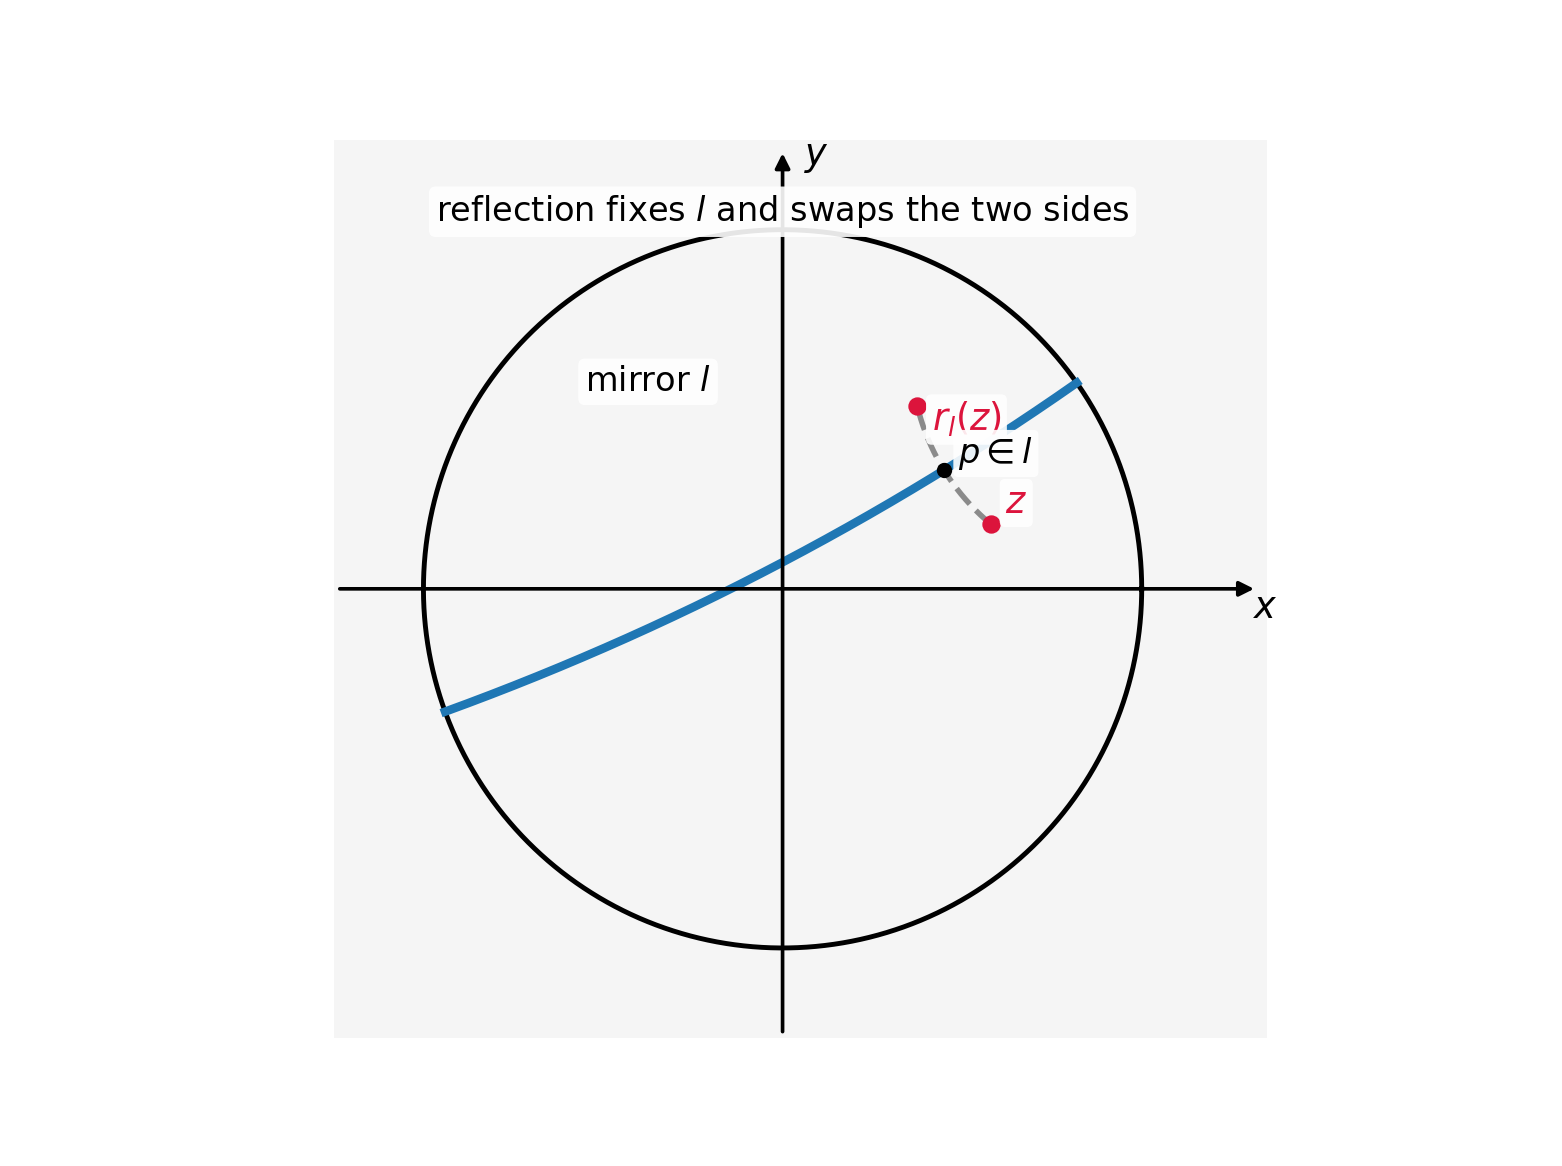
\includegraphics[width=0.72\textwidth]{chapters/part07_volume_vii/figures/poincare_reflection_in_line.png}
	\caption{Reflection $r_l$ in a hyperbolic line $l$ (Poincar\'e disk). The mirror $l$ is fixed pointwise and the perpendicular geodesic through $z$ meets $l$ at $p$, with $d_{\mathbb D}(z,l)=d_{\mathbb D}(r_l(z),l)$.}
\end{figure}

\begin{figure}[ht]
	\centering
	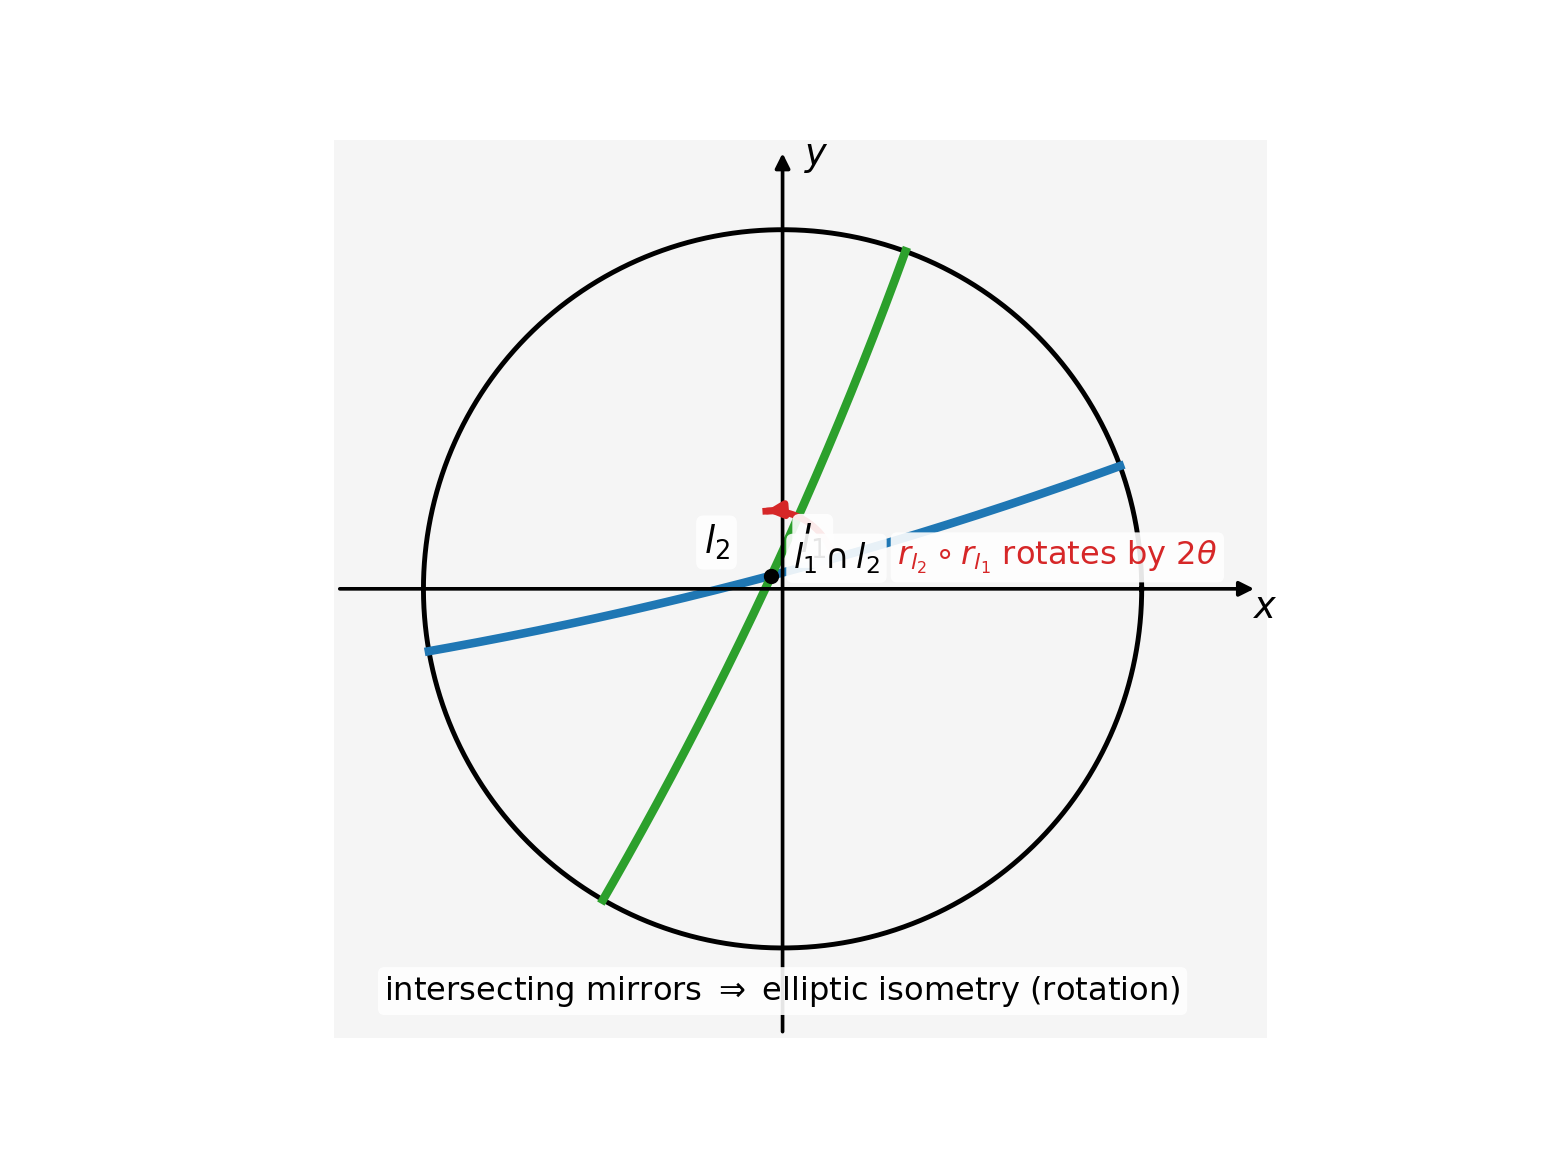
\includegraphics[width=0.72\textwidth]{chapters/part07_volume_vii/figures/poincare_intersecting_reflections.png}
	\caption{Two intersecting mirrors: if $l_1$ and $l_2$ meet at angle $\theta$, then $r_{l_2}\circ r_{l_1}$ is an elliptic isometry (a rotation) about $l_1\cap l_2$ by angle $2\theta$.}
\end{figure}


\par\medskip\noindent\textbf{Why the composition of two reflections rotates by $2\varphi$}\par\smallskip


Let $l_1$ and $l_2$ be two hyperbolic lines (geodesics) in the Poincar\'e disk model
that intersect at a point $P$, and let
\[
\varphi=\angle(l_1,l_2)\in(0,\pi)
\]
be their (hyperbolic) angle at $P$.
Since the Poincar\'e disk model is conformal, this equals the Euclidean angle at $P$.

Consider an oriented tangent ray $\rho$ based at $P$.
Let
\[
\alpha=\angle(\rho,l_1)
\]
be the signed angle from $l_1$ to $\rho$ (measured in $(-\pi,\pi)$).

\medskip
\noindent\textbf{Step 1: reflection in $l_1$.}
Reflection $r_{l_1}$ fixes $l_1$ pointwise and reverses orientation, hence it
\emph{negates} the signed angle with $l_1$:
\[
\angle\!\bigl(r_{l_1}(\rho),l_1\bigr)=-\alpha.
\]

\medskip
\noindent\textbf{Step 2: express angles with respect to $l_2$.}
Because $l_2$ is obtained from $l_1$ by rotating by $\varphi$ at $P$, we have
\[
\angle(\rho,l_2)=\alpha-\varphi,
\qquad
\angle\!\bigl(r_{l_1}(\rho),l_2\bigr)
=\angle\!\bigl(r_{l_1}(\rho),l_1\bigr)-\varphi
=-\alpha-\varphi.
\]

\medskip
\noindent\textbf{Step 3: reflection in $l_2$.}
Again reflection negates the signed angle with the mirror, so
\[
\angle\!\bigl(r_{l_2}r_{l_1}(\rho),\,l_2\bigr)
=
-\angle\!\bigl(r_{l_1}(\rho),\,l_2\bigr)
=
\alpha+\varphi.
\]

Finally convert back to angles with respect to $l_1$:
\[
\angle\!\bigl(r_{l_2}r_{l_1}(\rho),\,l_1\bigr)
=
\angle\!\bigl(r_{l_2}r_{l_1}(\rho),\,l_2\bigr)
+\varphi
=
(\alpha+\varphi)+\varphi
=
\alpha+2\varphi.
\]

\medskip
\noindent\textbf{Conclusion.}
For every tangent direction $\rho$ at $P$, the composition $r_{l_2}\circ r_{l_1}$
adds the constant angle $2\varphi$:
\[
\alpha \longmapsto \alpha+2\varphi.
\]
Therefore $r_{l_2}\circ r_{l_1}$ is a rotation about $P=l_1\cap l_2$ by angle $2\varphi$.

\medskip
\noindent\emph{Remark (answer to the confusion).}
The expression $\alpha+2\varphi$ is the \emph{final} angle of the ray with respect to $l_1$.
The \emph{rotation amount} is the difference
\[
(\alpha+2\varphi)-\alpha=2\varphi,
\]
which does \emph{not} depend on $\alpha$.

\end{solution}

\begin{problem}[CP-VII-0089 --- Problem 8 (Ideal square and hyperbolic surfaces)]
\label{prob:cp-vii-0089}
\begin{enumerate}
			\item Consider the \emph{ideal} hyperbolic square with vertices at $0,1,\infty,-1$ in the upper half--plane model.
			By gluing the edges of the square by isometries, or otherwise, prove that there is a \emph{complete} hyperbolic metric
			on the smooth surface $S^2\setminus\{p,q,r\}$ given by the complement of $3$ distinct points in the sphere.
			\item Construct a non-orientable compact hyperbolic surface.
		\end{enumerate}
\end{problem}

\begin{solution}
	Let $Q\subset\mathbb{H}$ be the ideal quadrilateral with vertices in cyclic order
	\[
	-1,\ 0,\ 1,\ \infty.
	\]
	Its sides are the geodesics:
	\[
	\ell_{-1}: x=-1,\qquad
	\ell_{1}: x=1,\qquad
	s_-:\text{ semicircle from }-1\text{ to }0,\qquad
	s_+:\text{ semicircle from }0\text{ to }1.
	\]
	
	\par\medskip\noindent\textbf{Step 1: choose explicit side-pairing isometries.}\par\smallskip

	Define the following isometries of $\mathbb{H}$:
	\[
	T(z)=z+2\quad(\text{translation}),\qquad
	R(z)=-\overline{z}\quad(\text{reflection in the imaginary axis}).
	\]
	Then:
	\[
	T(\ell_{-1})=\ell_1,\quad T(-1)=1,\quad T(\infty)=\infty,
	\]
	and
	\[
	R(s_+)=s_-,\quad R(0)=0,\quad R(1)=-1.
	\]
	Thus we can glue the sides by identifying $\ell_{-1}\sim\ell_1$ via $T$ and $s_+\sim s_-$ via $R$.
	
	\par\medskip\noindent\textbf{Step 2: identify the topology of the quotient.}\par\smallskip

	After gluing:
	\begin{itemize}
		\item the ideal vertex $\infty$ is fixed by $T$ and becomes a \emph{cusp end} (a puncture),
		\item the ideal vertices $-1$ and $1$ are identified by $T$ (also a cusp),
		\item the ideal vertex $0$ is fixed by $R$ (a cusp).
	\end{itemize}
	Hence the quotient has exactly three cusp ends. The resulting surface is connected and has Euler characteristic
	\[
	\chi = 2-3=-1,
	\]
	so it is homeomorphic to $S^2\setminus\{p,q,r\}$ (a sphere with three punctures), i.e. a \emph{pair of pants}.
	
	\par\medskip\noindent\textbf{Step 3: completeness of the induced hyperbolic metric.}\par\smallskip

	The metric on $Q$ is the restriction of the complete hyperbolic metric on $\mathbb{H}$.
	Gluing along geodesic sides by isometries produces a locally isometric quotient away from the ideal vertices.
	Near each ideal vertex one may take a horocyclic neighbourhood (a standard cusp neighbourhood); since the vertices are ideal,
	the distance to the vertex is infinite, and after gluing these neighbourhoods become standard cusp ends.
	Therefore the quotient metric is complete.
	
	\par\medskip\noindent\textbf{(Optional) Area check (Gauss--Bonnet / ideal polygon formula).}\par\smallskip

	An ideal $n$-gon in $\mathbb{H}$ has area $(n-2)\pi$. Here $n=4$, so
	\[
	\operatorname{Area}(Q)=2\pi.
	\]
	For the thrice-punctured sphere, $\chi=-1$, so Gauss--Bonnet gives
	\[
	\operatorname{Area} = -2\pi\chi = 2\pi,
	\]
	consistent with the construction.
	
	\par\medskip\noindent\textbf{Figure (colored): the ideal square and side pairings}\par\smallskip

	\begin{figure}[ht]
		\centering
		\begin{tikzpicture}[scale=3.2, line cap=round, line join=round]
			\fill[gray!8] (-1.25,0) rectangle (1.25,1.65);
			\draw[thick] (-1.25,0) -- (1.25,0);
			\draw[-{Latex[length=2mm]}, thick] (-1.25,0) -- (1.25,0) node[right] {$x$};
			\draw[-{Latex[length=2mm]}, thick] (0,0) -- (0,1.65) node[above] {$y$};
			\clip (-1.25,0) rectangle (1.25,1.65);
			
			% sides: x=-1 and x=1
			\draw[very thick, blue!70!black] (-1,0) -- (-1,1.65);
			\draw[very thick, blue!70!black] ( 1,0) -- ( 1,1.65);
			
			% semicircle from -1 to 0 (center -1/2, radius 1/2)
			\draw[very thick, red!70!black] (-1,0) arc[start angle=180, end angle=0, radius=0.5];
			
			% semicircle from 0 to 1 (center 1/2, radius 1/2)
			\draw[very thick, red!70!black] (0,0) arc[start angle=180, end angle=0, radius=0.5];
			
			% label ideal vertices
			\fill (-1,0) circle (0.02) node[below] {$-1$};
			\fill (0,0)  circle (0.02) node[below] {$0$};
			\fill (1,0)  circle (0.02) node[below] {$1$};
			\node at (0,1.58) {$\infty$};
			
			% pairing arrows: vertical sides via T(z)=z+2
			\draw[-{Latex[length=2mm]}, blue!70!black, thick] (-1,1.20) -- (1,1.20) node[midway, above] {\small $T:z\mapsto z+2$};
			
			% pairing arrows: semicircles via R(z)=-\bar z
			\draw[-{Latex[length=2mm]}, red!70!black, thick] (0.75,0.35) to[bend left=25] (-0.75,0.35)
			node[midway, above, fill=white, inner sep=1pt] {\small $R:z\mapsto -\bar z$};
			
			\node[fill=white, inner sep=1pt] at (0,1.02) {\small fundamental domain $Q$};
		\end{tikzpicture}
		\caption{An ideal quadrilateral with vertices $-1,0,1,\infty$ and one choice of side pairings producing the thrice-punctured sphere.}
	\end{figure}
	
	\par\medskip\noindent\textbf{Solution (b): a compact non-orientable hyperbolic surface}\par\smallskip

	A closed non-orientable surface of genus $k$ (connected sum of $k$ projective planes) has Euler characteristic
	\[
	\chi = 2-k.
	\]
	It admits a hyperbolic metric exactly when $\chi<0$, i.e. $k\ge 3$.
	
	\par\medskip\noindent\textbf{Concrete construction (genus $3$).}\par\smallskip

	Take a hyperbolic hexagon $P$ with interior angles
	\[
	\alpha=\frac{\pi}{3}
	\]
	(for example, a \emph{regular} hyperbolic hexagon with all sides equal and all angles $\pi/3$; such a polygon exists since
	$\alpha<\frac{(6-2)\pi}{6}=\frac{2\pi}{3}$).
	Label the sides consecutively as
	\[
	a,\ a,\ b,\ b,\ c,\ c,
	\]
	and glue each pair of equally-labeled sides by an isometry that reverses orientation along the boundary
	(so endpoints match). Because all six vertices are identified in the quotient, the total angle around the unique
	vertex is
	\[
	6\cdot \frac{\pi}{3}=2\pi,
	\]
	so the quotient has no cone singularity and inherits a smooth hyperbolic metric from $P$.
	
	The resulting surface has fundamental polygon word
	\[
	a^2\,b^2\,c^2,
	\]
	hence it is the connected sum of three projective planes: a closed non-orientable surface of genus $3$.
	Since $P$ is compact and the side pairings identify its boundary, the quotient is compact.
	
	\par\medskip\noindent\textbf{Area (Gauss--Bonnet check).}\par\smallskip

	For a closed hyperbolic surface,
	\[
	\operatorname{Area} = -2\pi\chi = 2\pi(k-2).
	\]
	For $k=3$ this gives $\operatorname{Area}=2\pi>0$, consistent with a hyperbolic metric.
	
	\par\medskip\noindent\textbf{Figure (colored schematic): side pairing for a non-orientable genus $3$ surface}\par\smallskip

	\begin{figure}[ht]
		\centering
		\begin{tikzpicture}[scale=2.0, line cap=round, line join=round]
			% Schematic hexagon (Euclidean-looking, used only to show identifications)
			\coordinate (V1) at (0:1.2);
			\coordinate (V2) at (60:1.2);
			\coordinate (V3) at (120:1.2);
			\coordinate (V4) at (180:1.2);
			\coordinate (V5) at (240:1.2);
			\coordinate (V6) at (300:1.2);
			
			\fill[gray!8] (V1) -- (V2) -- (V3) -- (V4) -- (V5) -- (V6) -- cycle;
			
			% edges in order: a,a,b,b,c,c
			\draw[very thick, red!70!black]   (V1) -- (V2);
			\draw[very thick, red!70!black]   (V2) -- (V3);
			
			\draw[very thick, blue!70!black]  (V3) -- (V4);
			\draw[very thick, blue!70!black]  (V4) -- (V5);
			
			\draw[very thick, green!60!black] (V5) -- (V6);
			\draw[very thick, green!60!black] (V6) -- (V1);
			
			% labels
			\node[red!70!black]   at ($(V1)!0.5!(V2)+(0.10,0.12)$) {$a$};
			\node[red!70!black]   at ($(V2)!0.5!(V3)+(0.15,0.00)$) {$a$};
			
			\node[blue!70!black]  at ($(V3)!0.5!(V4)+(-0.05,0.12)$) {$b$};
			\node[blue!70!black]  at ($(V4)!0.5!(V5)+(-0.15,0.00)$) {$b$};
			
			\node[green!60!black] at ($(V5)!0.5!(V6)+(-0.10,-0.12)$) {$c$};
			\node[green!60!black] at ($(V6)!0.5!(V1)+(0.10,-0.12)$) {$c$};
			
			% pairing arrows (schematic)
			\draw[-{Latex[length=2mm]}, red!70!black, thick]  ($(V1)!0.5!(V2)$) to[bend left=25] ($(V2)!0.5!(V3)$);
			\draw[-{Latex[length=2mm]}, blue!70!black, thick] ($(V3)!0.5!(V4)$) to[bend left=25] ($(V4)!0.5!(V5)$);
			\draw[-{Latex[length=2mm]}, green!60!black, thick]($(V5)!0.5!(V6)$) to[bend left=25] ($(V6)!0.5!(V1)$);
			
			\node[fill=white, inner sep=1pt] at (0,0) {\small word $a^2b^2c^2$ (non-orientable genus $3$)};
		\end{tikzpicture}
		\caption{Schematic side pairing on a hyperbolic hexagon producing a compact non-orientable hyperbolic surface (genus $3$).}
	\end{figure}
	
	\clearpage
	
	%=========================================================
	% Deep section: Ideal hyperbolic triangles (Theory + key computations)
	%=========================================================
	
	\par\medskip\noindent\textbf{Deep theory: Ideal hyperbolic triangles}\par\smallskip

	
	\par\medskip\noindent\textbf{Definition and basic picture}\par\smallskip

	An \emph{ideal hyperbolic triangle} is a hyperbolic triangle whose three vertices lie on the \emph{ideal boundary}
	\[
	\partial \mathbb{H}^2
	\]
	(e.g.\ in the upper half--plane model $\mathbb{H}=\{x+iy:y>0\}$ one has $\partial\mathbb{H}=\R\cup\{\infty\}$).
	Equivalently, it is a geodesic $3$--gon in $\mathbb{H}$ whose vertices are \emph{ideal points}.
	Such a triangle has:
	\begin{itemize}
		\item \textbf{Angles} $A=B=C=0$ (each vertex is at infinity),
		\item \textbf{Finite area} equal to $\pi$ (in curvature $-1$ normalization),
		\item \textbf{Infinite side lengths} (each side is a complete geodesic extending to the boundary),
		\item \textbf{Cusp ends} at each vertex: neighbourhoods of the vertices are \emph{cusps}.
	\end{itemize}
	
	\par\medskip\noindent\textbf{Uniqueness up to isometry}\par\smallskip

	Every ideal triangle in $\mathbb{H}^2$ is congruent to every other ideal triangle.
	
	\par\medskip\noindent\textbf{Reason (boundary $3$--transitivity).}\par\smallskip

	The full orientation-preserving isometry group of $\mathbb{H}$ is
	\[
	\operatorname{Isom}^+(\mathbb{H})\cong \operatorname{PSL}(2,\R),
	\]
	acting by M\\"{o}bius transformations
	\[
	z\longmapsto \frac{az+b}{cz+d},\qquad a,b,c,d\in\R,\ ad-bc=1.
	\]
	This action extends to the boundary $\partial\mathbb{H}=\R\cup\{\infty\}$ and is \emph{$3$--transitive} on distinct boundary points:
	given two triples of distinct boundary points $(u_1,u_2,u_3)$ and $(v_1,v_2,v_3)$ there exists a unique M\\"{o}bius map
	sending $u_i\mapsto v_i$ for $i=1,2,3$.
	Hence any ideal triangle can be mapped by an isometry to the \emph{standard ideal triangle} with vertices
	\[
	0,\ 1,\ \infty.
	\]
	
	\par\medskip\noindent\textbf{Standard ideal triangle in the upper half--plane}\par\smallskip

	Let $\Delta_{\mathrm{ideal}}$ be the triangle with vertices $0,1,\infty$.
	Its sides are the geodesics:
	\[
	\gamma_{0\infty}:\ x=0,\qquad
	\gamma_{1\infty}:\ x=1,\qquad
	\gamma_{01}:\ (x-\tfrac12)^2+y^2=\bigl(\tfrac12\bigr)^2,\ y>0.
	\]
	Thus it is bounded by two vertical lines and one semicircle orthogonal to $\R$.
	
	\par\medskip\noindent\textbf{Area of an ideal triangle}\par\smallskip

	For a hyperbolic triangle in curvature $-1$, Gauss--Bonnet gives
	\[
	\operatorname{Area}(\Delta)=\pi-(A+B+C).
	\]
	For an \emph{ideal} triangle $A=B=C=0$, therefore
	\[
	\operatorname{Area}(\Delta_{\mathrm{ideal}})=\pi.
	\]
	In particular, \emph{all} ideal triangles have area $\pi$, since they are all isometric.
	
	\par\medskip\noindent\textbf{Horocycles and cusp geometry}\par\smallskip

	A \emph{horocycle} in $\mathbb{H}$ is a curve orthogonal to all geodesics ending at a given ideal point.
	In the upper half--plane model:
	\begin{itemize}
		\item horocycles based at $\infty$ are horizontal lines $y=\text{const}$,
		\item horocycles based at a finite boundary point $a\in\R$ are Euclidean circles tangent to $\R$ at $a$.
	\end{itemize}
	
	If you cut an ideal triangle by horocycles near its vertices, you obtain a compact hexagon region.
	A fundamental and very useful fact is:
	
	\par\medskip\noindent\textbf{All ideal triangles are ``equilateral'' in horocyclic length.}\par\smallskip

	Choose one horocycle at each ideal vertex. Then the lengths of the three arcs of these horocycles inside the ideal triangle
	are all equal (with appropriate normalization of the horocycles). This expresses the strong symmetry of ideal triangles
	even though the vertices lie at infinity.
	
	
	%=========================================================
	% Horocycles ("horolines") inside an ideal triangle {1/4, 3/4, \infty}
	%=========================================================
% Requires: \usetikzlibrary{arrows.meta}

\begin{figure}[ht]
	\centering
	\begin{tikzpicture}[scale=5, line cap=round, line join=round]
		% background + real axis
		\fill[gray!8] (-0.10,0) rectangle (1.20,1.55);
		\draw[thick] (-0.10,0) -- (1.20,0);
		
		% axes
		\draw[-{Latex[length=2mm]}, thick] (-0.10,0) -- (1.20,0) node[right] {$x$};
		\draw[-{Latex[length=2mm]}, thick] (0,0) -- (0,1.55) node[above] {$y$};
		
		% parameters (triangle)
		\def\xa{0.25}
		\def\xb{0.75}
		\def\xc{0.50}
		\def\r{0.25}
		\def\ymax{1.55}
		
		% horocycle parameters
		\def\yinf{1.05}
		\def\rhL{0.18}
		\def\rhR{0.15}
		
		%-------------------------------------------------
		% Clip ONLY to the interior of the ideal triangle
		% rectangle [xa,xb]x[0,ymax] minus the disk (center xc,0 radius r)
		%-------------------------------------------------
		\begin{scope}
			\pgfseteorule
			\clip (\xa,0) rectangle (\xb,\ymax)
			(\xc,0) circle (\r);
			
			% shade interior
			\fill[cyan!18, opacity=0.28] (\xa,0) rectangle (\xb,\ymax);
			
			% horocycles (draw INSIDE the clipped interior)
			\draw[very thick, orange!85!black] (\xa,\yinf) -- (\xb,\yinf);      % at infinity
			\draw[very thick, violet!80!black] (\xa,\rhL) circle (\rhL);        % at 1/4
			\draw[very thick, teal!75!black]   (\xb,\rhR) circle (\rhR);        % at 3/4
		\end{scope}
		
		%-------------------------------------------------
		% Triangle sides on top (not clipped)
		%-------------------------------------------------
		\draw[very thick, blue!70!black] (\xa,0) -- (\xa,\ymax);
		\draw[very thick, blue!70!black] (\xb,0) -- (\xb,\ymax);
		\draw[very thick, red!70!black]  (\xa,0) arc[start angle=180, end angle=0, radius=\r];
		
		% vertices
		\fill (\xa,0) circle (0.02) node[below] {\scriptsize $\tfrac14$};
		\fill (\xb,0) circle (0.02) node[below] {\scriptsize $\tfrac34$};
		
		% infinity marker (inside)
		\draw[->, thin] (\xc,1.28) -- (\xc,1.40);
		\node[above, fill=white, inner sep=1pt, font=\scriptsize] at (\xc,1.40) {$\infty$};
		
		% short side labels (small, not intrusive)
		\node[blue!70!black, font=\scriptsize] at (\xa+0.03,1.18) {$x=\tfrac14$};
		\node[blue!70!black, font=\scriptsize] at (\xb-0.03,1.18) {$x=\tfrac34$};
		
		%-------------------------------------------------
		% OUTSIDE LEGEND + CALLOUTS (readable!)
		%-------------------------------------------------
		\node[anchor=west, fill=white, inner sep=2pt, font=\scriptsize]
		(Linf) at (0.86,1.52) {horocycle at $\infty$: $y=c$};
		\draw[->, thin, orange!85!black] (Linf.west) -- (\xb,\yinf);
		
		\node[anchor=west, fill=white, inner sep=2pt, font=\scriptsize]
		(L1) at (0.86,0.62) {horocycle at $\tfrac14$};
		\draw[->, thin, violet!80!black] (L1.west) -- (\xa,\rhL);
		
		\node[anchor=west, fill=white, inner sep=2pt, font=\scriptsize]
		(L2) at (0.86,0.48) {horocycle at $\tfrac34$};
		\draw[->, thin, teal!75!black] (L2.west) -- (\xb,\rhR);
		
		\node[anchor=west, fill=white, inner sep=2pt, font=\scriptsize]
		(Ltri) at (0.86,1.36) {ideal triangle $\{\tfrac14,\tfrac34,\infty\}$};
		
	\end{tikzpicture}
	
	\[
	(x-\tfrac12)^2+y^2=\bigl(\tfrac14\bigr)^2.
	\]
	
	\caption{Horocycles inside the ideal triangle $\{\tfrac14,\tfrac34,\infty\}$. Labels are moved to an external legend to keep the picture readable.}
\end{figure}

\par\medskip\noindent\textbf{Horocycles at $a=\tfrac14$ and the red geodesic side.}\par\smallskip

Consider the ideal triangle with vertices $\{\tfrac14,\tfrac34,\infty\}$ in the upper half--plane model.
Its ``red'' geodesic side (joining $\tfrac14$ to $\tfrac34$) is the semicircle
\[
(x-\tfrac12)^2+y^2=\Bigl(\tfrac14\Bigr)^2,\qquad (y>0).
\]
A horocycle based at $a=\tfrac14$ is a Euclidean circle tangent to $\R$ at $\tfrac14$, hence it has equation
\[
(x-\tfrac14)^2+(y-r)^2=r^2,\qquad r>0,
\]
with centre $\bigl(\tfrac14,r\bigr)$ and radius $r$.

\medskip

\noindent
\textbf{Key fact.}
A horocycle based at $a=\tfrac14$ \emph{always} meets the red geodesic side
\[
(x-\tfrac12)^2+y^2=\Bigl(\tfrac14\Bigr)^2.
\]
Thus there is no regime in which it ``does not cross the red boundary'' (except in the degenerate limiting sense as
the horocycle shrinks to the cusp point).

\par\medskip\noindent\textbf{1) What changes when the Euclidean radius $r$ increases?}\par\smallskip

As $r$ increases:
\begin{itemize}
	\item the circle becomes larger;
	\item its highest point is at $y=2r$ (directly above $x=\tfrac14$);
	\item near the real axis $y=0$ it becomes flatter (its curvature decreases), so parts of the circle may lie very close to $y=0$.
\end{itemize}
Hence ``larger radius'' does not mean ``the whole arc moves upward''; rather, the circle expands and flattens near the boundary.

\par\medskip\noindent\textbf{2) Explicit intersection with the red semicircle}\par\smallskip

Solve simultaneously
\[
(x-\tfrac14)^2+(y-r)^2=r^2,
\qquad
(x-\tfrac12)^2+y^2=\Bigl(\tfrac14\Bigr)^2.
\]
One intersection point is the cusp endpoint $(\tfrac14,0)$.
The second intersection point is
\[
x(r)=\frac{48r^2+1}{4(16r^2+1)},
\qquad
y(r)=\frac{2r}{16r^2+1}.
\]
Its limiting behaviour is:
\[
r\to 0:\quad (x(r),y(r))\to\Bigl(\tfrac14,0\Bigr),
\qquad
r\to\infty:\quad (x(r),y(r))\to\Bigl(\tfrac34,0\Bigr).
\]
So increasing $r$ makes the visible horocycle arc extend farther across the triangle, but the intersection height $y(r)$
eventually decreases back toward $0$.

\par\medskip\noindent\textbf{3) Why the arc looks cut in the picture (clipping to the triangle interior)}\par\smallskip

The interior of the ideal triangle $\{\tfrac14,\tfrac34,\infty\}$ is
\[
\operatorname{int}(\Delta)
=\Bigl\{\,x+iy\in\mathbb{H}:\ \tfrac14<x<\tfrac34,\ (x-\tfrac12)^2+y^2>\Bigl(\tfrac14\Bigr)^2\,\Bigr\}.
\]
Geometrically: we keep the region between the two vertical sides and \emph{outside} (above) the red semicircle.
Therefore, whenever part of the horocycle lies below the red semicircle, that part is \emph{not} in $\operatorname{int}(\Delta)$
and is clipped away; only the portion lying in the triangle interior remains visible.


	
	
	
	\par\medskip\noindent\textbf{Ideal triangle and the thrice-punctured sphere}\par\smallskip

	Gluing sides of an ideal polygon by isometries produces complete finite-area hyperbolic surfaces.
	The simplest example is the \emph{thrice-punctured sphere} (pair of pants with three cusps), which can be obtained from:
	\begin{itemize}
		\item two ideal triangles glued along their sides, or equivalently
		\item one ideal quadrilateral (as in Problem 8(a)) with suitable side pairings.
	\end{itemize}
	The total area equals $2\pi$, consistent with $\chi=-1$:
	\[
	\operatorname{Area} = -2\pi\chi = 2\pi.
	\]
	
	\par\medskip\noindent\textbf{Figure: the standard ideal triangle (colored)}\par\smallskip

	\begin{figure}[ht]
		\centering
		\begin{tikzpicture}[scale=4, line cap=round, line join=round]
			\fill[gray!8] (-0.2,0) rectangle (1.2,1.45);
			\draw[thick] (-0.2,0) -- (1.2,0);
			
			% axes
			\draw[-{Latex[length=2mm]}, thick] (-0.2,0) -- (1.2,0) node[right] {$x$};
			\draw[-{Latex[length=2mm]}, thick] (0,0) -- (0,1.45) node[above] {$y$};
			\clip (-0.2,0) rectangle (1.2,1.45);
			
			% sides x=0 and x=1
			\draw[very thick, blue!70!black] (0,0) -- (0,1.45);
			\draw[very thick, blue!70!black] (1,0) -- (1,1.45);
			
			% semicircle from 0 to 1: center 1/2 radius 1/2
			\draw[very thick, red!70!black] (0,0) arc[start angle=180, end angle=0, radius=0.5];
			
			% fill triangle region (visual)
			\path[fill=cyan!18, opacity=0.30]
			(0,0) -- (0,1.45) -- (1,1.45) -- (1,0)
			-- cycle;
			% clip fill to triangle by re-filling precisely:
			\begin{scope}
				\clip (0,0) -- (0,1.45) -- (1,1.45) -- (1,0) -- cycle;
				\fill[cyan!18, opacity=0.30]
				(0,0) arc[start angle=180, end angle=0, radius=0.5] -- cycle;
			\end{scope}
			
			% ideal vertices labels
% ideal vertices labels
\fill (0,0) circle (0.02) node[below] {$0$};
\fill (1,0) circle (0.02) node[below] {$1$};

% third ideal vertex (at infinity): show it clearly
\draw[->, thin] (0.5,1.24) -- (0.5,1.33);
\node[above, fill=white, inner sep=1pt] at (0.5,1.33) {$\infty$};
			
			\node[blue!70!black] at (0.08,1.18) {\small $x=0$};
			\node[blue!70!black] at (0.92,1.18) {\small $x=1$};
			\node[red!70!black]  at (0.50,0.25) {\small $(x-\tfrac12)^2+y^2=(\tfrac12)^2$};
			
			\node[fill=white, inner sep=1pt] at (0.5,1.08) {\small standard ideal triangle};
		\end{tikzpicture}
		\caption{The standard ideal hyperbolic triangle with vertices $0,1,\infty$ in the upper half--plane model. All ideal triangles are isometric and have area $\pi$.}
	\end{figure}
	
	\begin{itemize}
		\item The three sides are
		\[
		x=0,\qquad x=1,\qquad (x-\tfrac12)^2+y^2=\Bigl(\tfrac12\Bigr)^2 \quad (y>0).
		\]
		
		\item The \emph{interior} is the set of points in $\mathbb{H}$ that lie between the two vertical lines and
		outside (i.e.\ above) the semicircle:
		\[
		\operatorname{int}(\Delta)
		=\Bigl\{\,x+iy\in\mathbb{H}:\ 0<x<1,\ (x-\tfrac12)^2+y^2>\Bigl(\tfrac12\Bigr)^2\,\Bigr\}.
		\]
	\end{itemize}
	
	So: inside the triangle $=$ the region above the red semicircle, with $0<x<1$.
	
	\medskip
	
	Why ``outside the circle''? Because the side $\gamma_{01}$ \emph{is} the semicircle itself, and the ideal triangle is the
	unbounded region going upward toward the common ideal vertex $\infty$.
	
	% Requires: \usetikzlibrary{arrows.meta}
	\begin{figure}[ht]
		\centering
		\begin{tikzpicture}[scale=5, line cap=round, line join=round]
			\fill[gray!8] (-0.05,0) rectangle (1.05,1.45);
			\draw[thick] (-0.05,0) -- (1.05,0);
			
			% axes
			\draw[-{Latex[length=2mm]}, thick] (-0.05,0) -- (1.05,0) node[right] {$x$};
			\draw[-{Latex[length=2mm]}, thick] (0,0) -- (0,1.45) node[above] {$y$};
			\clip (-0.05,0) rectangle (1.05,1.45);
			
			% parameters
			\def\xa{0.25}
			\def\xb{0.75}
			\def\xc{0.50}
			\def\r{0.25}
			\def\ymax{1.45}
			
			% Fill interior region: rectangle between vertical sides minus the semicircle cap
			\path[fill=cyan!18, opacity=0.35, even odd rule]
			(\xa,0) -- (\xb,0) -- (\xb,\ymax) -- (\xa,\ymax) -- cycle
			(\xa,0) arc[start angle=180, end angle=0, radius=\r] -- cycle;
			
			% sides x=1/4 and x=3/4
			\draw[very thick, blue!70!black] (\xa,0) -- (\xa,\ymax);
			\draw[very thick, blue!70!black] (\xb,0) -- (\xb,\ymax);
			
			% semicircle from 1/4 to 3/4 (center 1/2, radius 1/4)
			\draw[very thick, red!70!black] (\xa,0) arc[start angle=180, end angle=0, radius=\r];
			
			% ideal vertices labels
			\fill (\xa,0) circle (0.02) node[below] {$\tfrac14$};
			\fill (\xb,0) circle (0.02) node[below] {$\tfrac34$};
			
			% the ideal vertex at infinity (shared endpoint of the two vertical geodesics)
			\draw[->, thin] (\xc,1.22) -- (\xc,1.33);
			\node[above, fill=white, inner sep=1pt] at (\xc,1.33) {$\infty$};
			
			% side labels
			\node[blue!70!black] at (\xa+0.03,1.18) {\small $x=\tfrac14$};
			\node[blue!70!black] at (\xb-0.03,1.18) {\small $x=\tfrac34$};
			\node[red!70!black]  at (\xc,0.27) {\small $(x-\tfrac12)^2+y^2=(\tfrac14)^2$};
			
			\node[fill=white, inner sep=1pt] at (\xc,1.05) {\small ideal triangle $\{\tfrac14,\tfrac34,\infty\}$};
		\end{tikzpicture}
		\caption{The ideal triangle with vertices $\{\tfrac14,\tfrac34,\infty\}$ in the upper half--plane model; its interior is shaded.}
	\end{figure}
	
	
	\par\medskip\noindent\textbf{Chat-style explanation (intuition, but still precise)}\par\smallskip

	\begin{itemize}
		\item Think of an ideal triangle as a triangle whose corners are ``pushed to infinity''. Each corner becomes a \emph{cusp}.
		\item Even though the sides run off to infinity, the triangle has a \emph{finite} area: exactly $\pi$.
		\item The reason everything is so rigid is that $\operatorname{PSL}(2,\R)$ can move any three boundary points to any other three:
		so there is only one ideal triangle shape.
		\item Ideal triangles are the basic building blocks of finite-area hyperbolic surfaces with cusps (like the thrice-punctured sphere).
	\end{itemize}
	
	\par\medskip\noindent\textbf{Deep theory: Ideal hyperbolic triangles in the Poincar\'e disk model}\par\smallskip

	
	\par\medskip\noindent\textbf{The Poincar\'e disk model.}\par\smallskip

	Let
	\[
	\mathbb{D}=\{z\in\C:\ |z|<1\}.
	\]
	The Poincar\'e metric (curvature $-1$) is
	\[
	ds^2_{\mathrm{hyp}}=\frac{4\,|dz|^2}{(1-|z|^2)^2}.
	\]
	The boundary circle $\partial\mathbb{D}=S^1=\{|z|=1\}$ is not part of the space, but it represents the \emph{ideal boundary}:
	points of $S^1$ are the \emph{ideal points} (points ``at infinity'').
	
	\par\medskip\noindent\textbf{Geodesics.}\par\smallskip

	Hyperbolic geodesics in $(\mathbb{D},d_{\mathrm{hyp}})$ are exactly:
	\begin{itemize}
		\item Euclidean diameters of the unit circle; and
		\item Euclidean circular arcs meeting $S^1$ \emph{orthogonally}.
	\end{itemize}
	(So the correct ``straight lines'' are those arcs that hit the boundary at right angles.)
	
	\par\medskip\noindent\textbf{Ideal triangles.}\par\smallskip

	An \emph{ideal hyperbolic triangle} is a region in $\mathbb{D}$ bounded by three geodesics whose endpoints lie on $S^1$,
	so its three vertices are ideal points $u,v,w\in S^1$ (pairwise distinct).
	
	\par\medskip\noindent\textbf{Uniqueness up to isometry.}\par\smallskip

	Every ideal triangle in $\mathbb{H}^2$ is congruent to every other one. In the disk model the orientation-preserving isometry group
	is the group of M\"obius transformations preserving $\mathbb{D}$ (often written $\mathrm{PSU}(1,1)\cong \mathrm{PSL}(2,\R)$),
	and it acts $3$-transitively on $S^1$: given two ordered triples of distinct boundary points, there is a unique isometry sending
	one triple to the other. Hence \emph{there are infinitely many ideal triangles in $\mathbb{D}$ as subsets, but only one up to isometry.}
	
	\par\medskip\noindent\textbf{Area.}\par\smallskip

	For a hyperbolic triangle with interior angles $A,B,C$ in curvature $-1$ one has
	\[
	\operatorname{Area}(\Delta)=\pi-(A+B+C).
	\]
	For an ideal triangle, $A=B=C=0$, so
	\[
	\operatorname{Area}(\Delta_{\mathrm{ideal}})=\pi.
	\]
	(So all ideal triangles have the same area $\pi$.)
	
	\par\medskip\noindent\textbf{Horocycles (horolines).}\par\smallskip

	In the disk model, a horocycle based at an ideal point $\xi\in S^1$ is a curve of constant distance from $\xi$,
	and it appears as a Euclidean circle \emph{tangent} to $S^1$ at $\xi$ (or, in the limiting case, a diameter/line in a suitable model).
	This is the disk analogue of ``$y=c$'' horocycles in the upper half-plane model.
	
	%=========================================================
	% Figure: Standard ideal triangle in the Poincar\\'{e} disk
	%=========================================================
	\begin{figure}[ht]
		\centering
		\begin{tikzpicture}[scale=3.2, line cap=round, line join=round]
			% background
			\fill[gray!6] (-1.25,-1.25) rectangle (1.35,1.25);
			
			% axes
			\draw[-{Latex[length=2mm]}, thick] (-1.25,0) -- (1.35,0) node[right] {$x$};
			\draw[-{Latex[length=2mm]}, thick] (0,-1.25) -- (0,1.25) node[above] {$y$};
			
			% unit disk boundary
			\draw[thick] (0,0) circle (1);
			
			% ideal vertices (cube roots of unity)
			\coordinate (A) at (1,0);
			\coordinate (B) at (-0.5,0.8660254);
			\coordinate (C) at (-0.5,-0.8660254);
			
			% fill ideal triangle interior by following geodesic arcs (orthogonal to S^1)
			% For this symmetric choice, each side is an arc of a circle of radius sqrt(3).
			\path[fill=cyan!18, opacity=0.35]
			(A) arc[start angle=-90, end angle=-150, radius=1.7320508]
			arc[start angle=30,  end angle=-30,  radius=1.7320508]
			arc[start angle=150, end angle=90,   radius=1.7320508]
			-- cycle;
			
			% draw the three geodesic sides (colored)
			\draw[very thick, red!70!black]
			(A) arc[start angle=-90, end angle=-150, radius=1.7320508];
			\draw[very thick, blue!70!black]
			(B) arc[start angle=30, end angle=-30, radius=1.7320508];
			\draw[very thick, green!60!black]
			(C) arc[start angle=150, end angle=90, radius=1.7320508];
			
			% mark ideal vertices on the boundary
			\fill (A) circle (0.02) node[below right] {$1$};
			\fill (B) circle (0.02) node[above left] {$e^{2\pi i/3}$};
			\fill (C) circle (0.02) node[below left] {$e^{4\pi i/3}$};
			
\node[fill=white, inner sep=2pt] at (0,0.12)
{\small ideal triangle in $(\mathbb{D},d_{\mathrm{hyp}})$};
		\end{tikzpicture}
		\caption{An ideal triangle in the Poincar\'e disk model. The sides are geodesics: Euclidean circle arcs orthogonal to the unit circle $S^1$. All ideal triangles are isometric and have area $\pi$.}
	\end{figure}
	
	
	% Requires: \usetikzlibrary{arrows.meta}
	
	\begin{figure}[ht]
		\centering
		\begin{tikzpicture}[scale=3.2, line cap=round, line join=round]
			% background + axes
			\fill[gray!6] (-1.25,-1.25) rectangle (1.45,1.25);
			\draw[-{Latex[length=2mm]}, thick] (-1.25,0) -- (1.45,0) node[right] {$x$};
			\draw[-{Latex[length=2mm]}, thick] (0,-1.25) -- (0,1.25) node[above] {$y$};
			
			% unit circle boundary of the disk
			\draw[thick] (0,0) circle (1);
			\node[below right] at (0.75,-0.75) {\small $\mathbb{D}=\{|z|<1\}$};
			
			%--------------------------------------------
			% Type 1: a diameter geodesic
			%--------------------------------------------
			\def\angD{25} % angle for diameter
			\coordinate (D1) at ({cos(\angD)},{sin(\angD)});
			\coordinate (D2) at ({-cos(\angD)},{-sin(\angD)});
			\draw[very thick, purple!75!black] (D2) -- (D1);
			\node[fill=white, inner sep=2pt, font=\scriptsize] at (0.15,0.55)
			{geodesic type 1: diameter};
			
			%--------------------------------------------
			% Type 2: orthogonal arc geodesic (right side)
			% Endpoints at angles \\ensuremath{\\pm}60\\textdegree{} on S^1:
			% center a = sec(60)=2 on x-axis, radius R = tan(60)=sqrt(3)
			% Param: x = a + R cos t, y = R sin t, with t in [180-\\ensuremath{\\theta},180+\\ensuremath{\\theta}]
			%--------------------------------------------
			\def\thetaR{60}
			\def\aR{2.0}
			\def\RR{1.7320508}
			\draw[very thick, red!70!black]
			plot[smooth, variable=\t, domain={180-\thetaR}:{180+\thetaR}, samples=220]
			({\aR+\RR*cos(\t)},{\RR*sin(\t)});
			% optional: show the full supporting circle (dashed) to emphasize orthogonality
			\draw[dashed, red!70!black, opacity=0.45] (\aR,0) circle (\RR);
			\node[fill=white, inner sep=2pt, font=\scriptsize] at (0.55,0.15)
			{geodesic type 2: arc $\perp\,S^1$};
			
			%--------------------------------------------
			% Another orthogonal arc (left side)
			% Choose \\ensuremath{\\theta}=50\\textdegree{}, endpoints at angles 180\\ensuremath{\\pm}50\\textdegree{}; center a=-sec(50), radius=tan(50)
			% For this case the inside-disk arc is t in [-(90-\\ensuremath{\\theta}), +(90-\\ensuremath{\\theta})].
			%--------------------------------------------
			\def\thetaL{50}
			\def\aL{-1.5557238}  % -sec(50\\textdegree{})
			\def\RL{1.1917536}   % tan(50\\textdegree{})
			\draw[very thick, blue!70!black]
			plot[smooth, variable=\t, domain={-(90-\thetaL)}:{(90-\thetaL)}, samples=220]
			({\aL+\RL*cos(\t)},{\RL*sin(\t)});
			\draw[dashed, blue!70!black, opacity=0.45] (\aL,0) circle (\RL);
			
			%--------------------------------------------
			% (Optional) Non-example: a Euclidean circle NOT tangent/orthogonal to S^1
			%--------------------------------------------
			\draw[densely dashed, gray!70] (0.25,0.15) circle (0.32);
			\node[gray!70, font=\scriptsize] at (0.25,-0.25) {not a geodesic};
			
			% mark a couple of boundary points (endpoints live on S^1)
			\fill (1,0) circle (0.015);
			\fill (-1,0) circle (0.015);
			\node[font=\scriptsize, above right] at (1,0) {$S^1$};
		\end{tikzpicture}
		\caption{Poincar\'e-disk geodesics: diameters and circular arcs orthogonal to \(S^1\).}
	\end{figure}
	
	\clearpage
	
\par\medskip\noindent\textbf{E1. Constellations of circles and M\"obius transformations}\par\smallskip

\end{solution}

\subsection*{Main-text correspondence: VII/36}

\begin{problem}[CP-VII-0090 --- \(\mathrm{PSL}(2,\mathbb{C})\), boundary dilation, and an isometry of \(\mathbb{H}^3\)]
\label{prob:cp-vii-0090}
Use the upper-half-space model
\[
\mathbb{H}^3
=
\{(z,t)\in\mathbb{C}\times\mathbb{R}_{>0}\},
\qquad
ds^2=\frac{|dz|^2+dt^2}{t^2}.
\]
For \(s\in\mathbb{R}\), consider
\[
A_s=
\begin{pmatrix}
e^{s/2}&0\\
0&e^{-s/2}
\end{pmatrix}
\in \mathrm{SL}(2,\mathbb{C}).
\]

\begin{enumerate}
\item Compute the M\\"{o}bius transformation induced by \(A_s\) on the
      boundary \(\widehat{\mathbb{C}}\).
\item Show directly that
      \[
      F_s(z,t)=(e^s z,e^s t)
      \]
      is an isometry of \(\mathbb{H}^3\).
\item Show that the vertical geodesic \(\gamma(t)=(0,t)\) is preserved,
      and compute the hyperbolic distance from \((0,1)\) to \((0,e^s)\).
\end{enumerate}
\end{problem}

\begin{solution}
The M\\"{o}bius action is
\[
z\longmapsto
\frac{e^{s/2}z}{e^{-s/2}}
=e^s z.
\]

Under \(F_s\),
\[
dz\longmapsto e^s dz,
\qquad
dt\longmapsto e^s dt,
\qquad
t\longmapsto e^s t.
\]
Therefore
\[
F_s^*ds^2
=
\frac{e^{2s}|dz|^2+e^{2s}dt^2}{e^{2s}t^2}
=
\frac{|dz|^2+dt^2}{t^2}.
\]
Thus \(F_s\) is an isometry.

The set \(z=0\) is invariant under \(F_s\).  Along this vertical
geodesic the line element is
\[
ds=\frac{dt}{t}.
\]
Hence
\[
d_{\mathbb H^3}\bigl((0,1),(0,e^s)\bigr)
=
\left|\int_1^{e^s}\frac{dt}{t}\right|
=
|s|.
\]
Thus this diagonal element of \(\mathrm{PSL}(2,\mathbb C)\) acts as a
hyperbolic translation along the vertical axis, while its boundary
action is the dilation \(z\mapsto e^s z\).
\end{solution}

\subsection*{Main-text correspondence: VII/37}

\begin{problem}[CP-VII-0091 --- A loxodromic cyclic Kleinian group and its limit set]
\label{prob:cp-vii-0091}
Let \(\lambda\in\mathbb{C}\) satisfy \(|\lambda|>1\), and let
\[
T(z)=\lambda z
\]
act on the Riemann sphere \(\widehat{\mathbb{C}}\).  Let
\(\Gamma=\langle T\rangle\subset\mathrm{PSL}(2,\mathbb{C})\).

\begin{enumerate}
\item Determine the fixed points of \(T\).
\item For \(z\in\mathbb{C}^{\times}\), determine the limits of
      \(T^n(z)\) as \(n\to+\infty\) and as \(n\to-\infty\).
\item Show that the limit set of the cyclic Kleinian group \(\Gamma\) is
      \[
      \Lambda(\Gamma)=\{0,\infty\}.
      \]
\item Identify the domain of discontinuity
      \(\Omega(\Gamma)=\widehat{\mathbb{C}}\setminus\Lambda(\Gamma)\).
\end{enumerate}
\end{problem}

\begin{solution}
The equation \(T(z)=z\) gives \((\lambda-1)z=0\), hence \(z=0\);
the point \(\infty\) is also fixed.  Thus the two fixed points are
\(0\) and \(\infty\).

For \(z\ne0,\infty\),
\[
T^n(z)=\lambda^n z.
\]
Since \(|\lambda|>1\),
\[
T^n(z)\longrightarrow\infty\qquad(n\to+\infty),
\]
whereas
\[
T^n(z)\longrightarrow0\qquad(n\to-\infty).
\]
Consequently every orbit in \(\mathbb C^\times\) accumulates only at
\(0\) and \(\infty\), and both points occur as accumulation points.
Hence
\[
\boxed{\Lambda(\Gamma)=\{0,\infty\}}.
\]
The domain of discontinuity is therefore
\[
\boxed{\Omega(\Gamma)=\widehat{\mathbb C}\setminus\{0,\infty\}
      =\mathbb C^\times}.
\]
This is the simplest model of the boundary dynamics of a loxodromic
cyclic Kleinian group.
\end{solution}

\section{Computational Geometry}

\subsection*{Main-text correspondence: VII/38}

\begin{problem}[CP-VII-0092 --- Why edge-graph shortest paths zig-zag on a triangular mesh]
\label{prob:cp-vii-0092}
Let a triangulated polyhedral surface approximate a smooth surface.
Suppose a shortest-path solver is restricted to the mesh vertex--edge graph.

\begin{enumerate}
\item Explain why Dijkstra's algorithm on this graph computes the shortest
path only among edge-constrained paths, not among all curves on the
polyhedral surface.
\item Give a geometric reason why a coarse or anisotropic triangulation can
produce a visible zig-zag or staircasing artifact.
\item Explain why adding local face-crossing shortcuts can reduce the artifact
without making the method exact.
\end{enumerate}
\end{problem}

\begin{solution}
Dijkstra's algorithm minimizes the sum of graph-edge weights among graph
paths.  If the graph consists only of mesh vertices and mesh edges, every
admissible path must follow edges.  A true polyhedral geodesic, however, may
cross the interior of triangle faces, so the graph optimum need not be the
surface optimum.

On a coarse mesh, available edge directions form a sparse directional set.
A path that should locally travel in an intermediate direction is forced to
alternate between nearby edge directions.  This produces the characteristic
zig-zag appearance.  The effect becomes more pronounced when triangles are
poorly shaped or strongly aligned.

Adding face diagonals, two-ring connections, or local shortcuts enriches the
set of admissible directions, so the graph path can better approximate a
face-crossing geodesic.  Nevertheless the solution is still restricted to
the chosen discrete graph.  It can therefore cut corners incorrectly or miss
the exact polyhedral shortest path.
\end{solution}

\subsection*{Main-text correspondence: VII/39}

\begin{problem}[CP-VII-0093 --- Graph approximations versus exact polyhedral geodesics]
\label{prob:cp-vii-0093}
Consider two points \(p,q\) on a triangulated polyhedral surface.

\begin{enumerate}
\item State the essential difference between an edge-graph Dijkstra/A*
distance and an exact polyhedral geodesic distance.
\item Explain what an exact method must allow when the path crosses a sequence
of triangular faces.
\item Compare, at a conceptual level, graph-based methods with classical exact
methods such as Chen--Han and Mitchell--Mount--Papadimitriou (MMP).
\end{enumerate}
\end{problem}

\begin{solution}
An edge-graph method minimizes over a finite graph.  Its admissible curves are
therefore constrained by the graph connectivity.  The exact polyhedral
geodesic distance minimizes over all curves on the piecewise-flat surface.

Inside each triangular face the exact shortest path is a straight Euclidean
segment in that face.  Across adjacent faces, one may unfold the triangles
isometrically into the plane; a geodesic segment then continues as a straight
line in the unfolded development, subject to the combinatorics of the crossed
faces and possible interactions with vertices.

Graph methods are simple, robust, and fast, but generally approximate.
Chen--Han and MMP propagate exact shortest-path information across the
polyhedral surface and recover the true polyhedral distance, but require
substantially more geometric bookkeeping and are harder to implement robustly.
Thus the tradeoff is principally implementation simplicity versus exactness on
the mesh surface.
\end{solution}

\subsection*{Main-text correspondence: VII/40}

\begin{problem}[CP-VII-0094 --- Heat and front-propagation methods for geodesic distance]
\label{prob:cp-vii-0094}
Let \(M\) be a triangulated surface and \(s\) a source vertex.

\begin{enumerate}
\item Describe the three conceptual stages of the Heat Method for approximating
geodesic distance from \(s\).
\item Explain how Fast Marching differs conceptually from the Heat Method.
\item Why can an intrinsic Delaunay triangulation improve the numerical
behavior of either distance computation on a poor-quality mesh?
\end{enumerate}
\end{problem}

\begin{solution}
The Heat Method uses the principle that short-time heat flow points in the
direction of steepest decrease of geodesic distance.

First solve a short-time heat equation, typically in discrete form
\[
(M+tL)u=M\delta_s,
\]
where \(M\) is a mass matrix and \(L\) a discrete Laplacian.
Next form the normalized vector field
\[
X=-\frac{\nabla u}{|\nabla u|}.
\]
Finally recover a scalar potential \(\phi\) by solving a Poisson problem
\[
L\phi=\operatorname{div}X.
\]
After adding a constant so that \(\phi(s)=0\), the function \(\phi\)
approximates geodesic distance.

Fast Marching instead propagates an advancing front while enforcing a
discrete analogue of the eikonal equation
\[
|\nabla d|=1.
\]
It is therefore a causal front-propagation method rather than a sequence of
global elliptic solves.

Poorly shaped triangles can degrade discrete differential operators and front
updates.  Replacing the mesh connectivity by an intrinsic Delaunay
triangulation improves angle quality in the intrinsic metric and yields better
behaved cotangent weights and propagation geometry, often increasing stability
without changing the underlying polyhedral metric.
\end{solution}

\subsection*{Main-text correspondence: VII/41}

\begin{problem}[CP-VII-0095 --- The cotangent Laplacian and its quadratic energy]
\label{prob:cp-vii-0095}
Let a triangulated surface have symmetric cotangent weights
\[
w_{ij}=\frac12\bigl(\cot\alpha_{ij}+\cot\beta_{ij}\bigr)
\]
on every interior edge \(ij\).  Define the stiffness-form discrete
Laplacian \(L\) by
\[
L_{ij}=-w_{ij}\quad(i\ne j),
\qquad
L_{ii}=\sum_{j\sim i}w_{ij}.
\]

\begin{enumerate}
\item Show that every row of \(L\) sums to zero.
\item Deduce that constant vertex functions lie in the kernel of \(L\).
\item Prove
      \[
      f^{\mathsf T}Lf
      =
      \sum_{\{i,j\}}w_{ij}(f_i-f_j)^2,
      \]
      where each unoriented edge is counted once.
\item If all relevant triangles are equilateral, compute \(w_{ij}\).
\end{enumerate}
\end{problem}

\begin{solution}
For a fixed vertex \(i\),
\[
\sum_j L_{ij}
=
L_{ii}+\sum_{j\sim i}L_{ij}
=
\sum_{j\sim i}w_{ij}-\sum_{j\sim i}w_{ij}
=0.
\]
Hence, for the constant vector \(\mathbf 1\),
\[
L\mathbf 1=0.
\]

Using the symmetry \(w_{ij}=w_{ji}\),
\[
\begin{aligned}
f^{\mathsf T}Lf
&=
\sum_i\left(\sum_{j\sim i}w_{ij}\right)f_i^2
-\sum_i\sum_{j\sim i}w_{ij}f_if_j\\
&=
\sum_{\{i,j\}}w_{ij}
\bigl(f_i^2+f_j^2-2f_if_j\bigr)\\
&=
\sum_{\{i,j\}}w_{ij}(f_i-f_j)^2.
\end{aligned}
\]
Thus the stiffness energy is nonnegative whenever the cotangent weights
are nonnegative.

For equilateral triangles,
\[
\alpha_{ij}=\beta_{ij}=\frac{\pi}{3},
\qquad
\cot\frac{\pi}{3}=\frac1{\sqrt3}.
\]
Therefore
\[
\boxed{w_{ij}=\frac1{\sqrt3}}.
\]
\end{solution}

\subsection*{Main-text correspondence: VII/42}

\begin{problem}[CP-VII-0096 --- Principal directions, curvature lines, ridges, and valleys]
\label{prob:cp-vii-0096}
Let \(S\subset\mathbb{R}^3\) be a smooth oriented surface, and suppose
\(p\in S\) is non-umbilic with principal curvatures
\[
k_1(p)>k_2(p)
\]
and corresponding unit principal directions \(e_1,e_2\).

\begin{enumerate}
\item Explain why the integral curves of \(e_1\) and \(e_2\) are curvature
lines away from umbilics.
\item A common local ridge criterion for the larger principal curvature is
\[
D_{e_1}k_1=0,
\qquad
D_{e_1}^2k_1<0.
\]
Interpret these two conditions geometrically.
\item State the analogous local valley criterion.
\item For a circular cylinder of radius \(R\), determine the principal
curvatures and explain why this strict ridge/valley test does not isolate
special ridge or valley curves.
\end{enumerate}
\end{problem}

\begin{solution}
At a non-umbilic point the shape operator has two distinct eigenvalues, so its
unit eigenvector fields \(e_1,e_2\) are locally defined up to sign.  Curves
whose tangent vectors agree with one of these principal fields are, by
definition, curvature lines.

The equation
\[
D_{e_1}k_1=0
\]
says that \(k_1\) is stationary when moving in its own principal direction.
The inequality
\[
D_{e_1}^2k_1<0
\]
says that this stationary value is a strict local maximum in that direction.
Thus the point lies on a local ridge associated with the larger principal
curvature.

The corresponding valley criterion is
\[
D_{e_1}k_1=0,
\qquad
D_{e_1}^2k_1>0,
\]
for a local minimum in the same principal direction.  Equivalent conventions
may instead be formulated using the smaller principal curvature.

For a circular cylinder,
\[
k_1=\frac1R,
\qquad
k_2=0
\]
up to the sign determined by orientation.  Both are constant, so all first
and second directional derivatives of \(k_1\) vanish.  Hence the strict
second-derivative inequalities required by the ridge/valley test fail:
the cylinder has principal-direction foliations, but no isolated strict
ridge or valley curves under this criterion.
\end{solution}
